% =====================================================================
% labbook/main.tex — MASTER of the sharded LaTeX labbook (TJO directive
% 2026-08-30). ROLE: preamble + macros + an ORDERED \include list ONLY.
% No body prose and no \section in this file.
%
% PURPOSE: a complete, self-contained, READABLE record of every result of
% the campaign. A reader must never need to look up a campaign acronym:
% every definition is restated in full, every result carries a descriptive
% human name, and campaign identifiers appear only as provenance metadata.
%
% LOCKSTEP RULE: any commit that changes a status in claims/CLAIMS.md or
% adds/edits a definition in definitions.md MUST update the corresponding
% shard here in the same commit. scripts/check-labbook.sh verifies that
% every claim id and definition number appears in some shard.
%
% Build: cd labbook && make      (latexmk -pdf main.tex -> main.pdf)
% =====================================================================
\documentclass[11pt]{article}

\usepackage[margin=1in]{geometry}
\usepackage{amsmath,amssymb,amsthm,mathtools}
\usepackage{array,booktabs,longtable}
\usepackage{bm}
\usepackage{graphicx}
\usepackage[dvipsnames]{xcolor}
\usepackage[hidelinks]{hyperref}
\usepackage[capitalise,noabbrev]{cleveref}

% ---------------------------------------------------------------------
% Theorem environments (numbered within sections)
% ---------------------------------------------------------------------
\theoremstyle{plain}
\newtheorem{theorem}{Theorem}[section]
\newtheorem{proposition}[theorem]{Proposition}
\newtheorem{lemma}[theorem]{Lemma}
\newtheorem{corollary}[theorem]{Corollary}
\newtheorem{conjecture}[theorem]{Conjecture}
\newtheorem{refutedclaim}[theorem]{Refuted claim}
\theoremstyle{definition}
\newtheorem{definition}[theorem]{Definition}
\newtheorem{observation}[theorem]{Observation}
\newtheorem{oracle}[theorem]{Oracle fact}
\theoremstyle{remark}
\newtheorem{remark}[theorem]{Remark}
\newtheorem{scope}[theorem]{Scope}

% ---------------------------------------------------------------------
% Status tags. Usage: \statusProved, \statusSketch, \statusConjecture,
% \statusRefuted, and \statusProvedConditional for conditional theorems.
% The tag ALWAYS matches the status column of claims/CLAIMS.md.
% ---------------------------------------------------------------------
\newcommand{\statustag}[2]{\textcolor{#1}{\textup{\textsc{\small [#2]}}}}
\newcommand{\statusProved}{\statustag{ForestGreen}{proved}}
\newcommand{\statusProvedConditional}{\statustag{ForestGreen}{proved, conditional}}
\newcommand{\statusSketch}{\statustag{Orange}{sketch}}
\newcommand{\statusConjecture}{\statustag{RoyalBlue}{conjecture}}
\newcommand{\statusRefuted}{\statustag{BrickRed}{refuted}}

% ---------------------------------------------------------------------
% Provenance block. Four arguments:
%   1. campaign identifier(s) (claims/CLAIMS.md row id, or D-number)
%   2. where proved / stated (repo file + step anchor)
%   3. where tested (checker / numerics), or --- if none
%   4. review record (verdict file / adjudication), or --- if none
% Renders as a quiet footnotesize block after the statement. This is the
% ONLY place campaign ids are load-bearing; body text never relies on them.
% ---------------------------------------------------------------------
\newcommand{\provenance}[4]{%
  \par\nobreak\vspace{0.25\baselineskip}%
  {\footnotesize\color{gray}%
   \begin{tabular}{@{}p{0.16\textwidth}@{}p{0.80\textwidth}@{}}
     campaign id: & #1 \\
     proved in:   & #2 \\
     tested by:   & #3 \\
     reviewed in: & #4 \\
   \end{tabular}\par}%
  \vspace{0.25\baselineskip}}

% ---------------------------------------------------------------------
% Semantic macros (mirror notation.md; single source of typesetting)
% ---------------------------------------------------------------------
\newcommand{\braket}[1]{\langle #1\rangle}
\newcommand{\ket}[1]{|#1\rangle}
\newcommand{\bra}[1]{\langle #1|}
\newcommand{\norm}[1]{\lVert #1\rVert}
\newcommand{\abs}[1]{\lvert #1\rvert}
\DeclareMathOperator{\spec}{spec}
\DeclareMathOperator{\ran}{ran}
\DeclareMathOperator{\sgn}{sgn}
\DeclareMathOperator{\dist}{dist}
\DeclareMathOperator{\supp}{supp}
\DeclareMathOperator{\Ad}{Ad}
\DeclareMathOperator{\Hom}{Hom}
\DeclareMathOperator{\Inv}{Inv}
\newcommand{\Z}{\mathbb{Z}}
\newcommand{\R}{\mathbb{R}}
\newcommand{\C}{\mathbb{C}}
\newcommand{\N}{\mathbb{N}}
\newcommand{\A}{\mathcal{A}}            % asymptotic symmetry group (script A)
\newcommand{\Hilb}{\mathcal{H}}
\newcommand{\Kk}{\mathcal{K}}           % kink sector space
\newcommand{\alg}{\mathfrak{A}}         % quasi-local algebra
\newcommand{\softS}{\mathsf{S}}         % the soft multiplier of D25
\newcommand{\classSW}{\mathcal{S}_W}    % the no-contact universality class
\newcommand{\aleg}{\mathfrak{a}_{\mathrm{leg}}} % soft-leg amputation constant
\newcommand{\Qhat}{\hat{Q}}             % windowed regularised charge
\newcommand{\wallX}{\mathfrak{X}}       % windowed wall-position observable

\title{The infrared triangle on the lattice:\\ the campaign labbook}
\author{Repository \texttt{tns-as-st-me}; owner Tobias Osborne}
\date{\today\ (maintained in lockstep with \texttt{claims/CLAIMS.md})}

\begin{document}
\maketitle
\tableofcontents

% SHARD-ID: LB-00-OVERVIEW
% SHARD-TITLE: Overview -- the lattice infrared triangle
% SHARD-SOURCES: HANDOFF_MPS_SOFT_THEOREM.md; PRD.md; paper/skeleton.md;
%   HANDOFF.md; claims/CLAIMS.md (statuses quoted, not restated); CLAUDE.md
%   (laws L1--L10); labbook/WRITING-GUIDE.md
% SHARD-CLAIMS: none owned.  This shard states no theorem and therefore
%   carries no provenance block; every result it mentions is named in
%   English and cross-referenced to the section that owns it.

\section{Overview: the lattice infrared triangle}
\label{sec:overview}

\subsection{What the continuum triangle is}

In four-dimensional quantum field theory three families of statements that
look unrelated turn out to be one statement seen from three sides. The first
family is the \emph{soft theorems}: when one massless quantum in a scattering
process has its frequency taken to zero, the amplitude factorises into a
universal kinematic multiplier times the amplitude without that quantum. The
second is the \emph{asymptotic symmetries}: transformations that act
nontrivially on the data at null or spatial infinity, taken modulo those that
die off there, form a genuine symmetry group of the theory rather than a
gauge redundancy. The third is the \emph{memory effects}: after a burst of
radiation has passed, detectors do not return to their initial configuration
but retain a permanent, zero-frequency offset. The triangle is the assertion
that the soft theorem is the Ward identity of the asymptotic symmetry, and
that the memory is the Fourier-zero-mode content of the same Ward identity.
Each edge is a change of variables, not a new physical input.

Two features of that story matter for what follows. First, the triangle is,
in the continuum, a family of formal relations: the asymptotic symmetry
algebra is defined through boundary conditions at infinity whose function
spaces are delicate, and the soft factorisation is an all-orders statement
about an S-matrix that is not itself constructed. Second, there are two quite
different versions of it. The version usually advertised is the gauge one
(photons, gravitons), in which the soft factor has a $1/\omega$ pole because
a massless mediator is exchanged. The version relevant here is the
\emph{global} one: the soft-pion, or Goldstone, triangle, in which the soft
factor has no pole at all but an \emph{Adler zero} --- it vanishes linearly
as the momentum goes to zero, because the zero-momentum Goldstone mode is
exactly a global symmetry rotation of the vacuum and therefore acts trivially.

\subsection{Why the lattice version must be the Goldstone one}

This campaign asks whether the triangle is a theorem anywhere, and answers
the question on a one-dimensional quantum spin chain written in
matrix-product-state (MPS) language. There the three corners become finite,
checkable statements about tensors: the symmetry acts on-site, the vacua are
injective MPS, the excitations are ansatz vectors, and the Ward identity is
an exact algebraic rearrangement of a tensor network.

The gauge triangle has no home here. A one-dimensional lattice spin system
carries no massless gauge mediator --- the natural candidate, the Schwinger
model, confines and gives its photon a mass --- so there is no mechanism for
a $1/\omega$ pole, and any claim of one in this setting is simply wrong. The
correct antecedent is the global-symmetry triangle: the soft object is a
Goldstone-like magnon, the expected behaviour is an Adler zero, and the
leading soft datum is a \emph{slope} rather than a residue. Two further
structural facts fix the setting. Mermin--Wagner and Coleman forbid
continuous type-A symmetry breaking in a one-dimensional ground state, so the
triangle must live either on a type-B Goldstone (the isotropic Heisenberg
ferromagnet, exact product vacuum, magnon dispersion $\omega\sim k^2$, exact
Bethe scattering data available as an independent oracle) or on a discretely
broken symmetry (the easy-axis XXZ ferromagnet, two product vacua, domain
walls, gapped magnons, so that ``soft'' means a low-frequency expansion about
the gap). And there are no boosts on a lattice, so the universal factor
cannot take a Lorentz-covariant form; its correct dependence on the legs'
group velocities is part of the problem rather than an obstacle to it.

The two model classes are used throughout. The ferromagnetic chain supplies
exact magnons and an exact two-body scattering matrix; the easy-axis chain
supplies exact kinks and a wall-position observable whose displacement is the
memory. Neither model alone exhibits every corner, and that tension is
structural: it is respected in what follows, not papered over.

\subsection{The four headline findings}

\paragraph{(i) Memory quantization needs no scattering theory.}
The naive expectation, inherited from the continuum, is that the memory is
quantized because it is the zero-frequency limit of a soft factor, so that
one must first have a soft theorem and an S-matrix before one can say
anything about the permanent displacement. That expectation is wrong here,
and its failure is the campaign's most robust positive result. Fix a finite
window $W=[a,b]$ of the chain, a cut $c_0\in W$, and the windowed
wall-position observable
\begin{equation}
  \wallX_W \;=\; a-1+\frac{1}{2s}\sum_{x=a}^{b}\bigl(S^z_x+s\bigr),
  \qquad
  \Qhat_{W,c_0} \;=\; 2s\bigl(\wallX_W-c_0\bigr),
  \label{eq:ov-window-charge}
\end{equation}
where $\pm s$ are the charge densities of the two vacua. If the on-site
charge merely generates a circle --- that is, if $e^{2\pi i S^z_x}$ is a
scalar, which holds for every spin-$S$ chain --- then the spectrum of
$\Qhat_{W,c_0}$ lies in a single coset of $\Z$, and the increment recorded by
measuring this same observable before and after an event is an
\emph{integer}. No wave operators, no channel inventory, no completeness, no
gap, no Lieb--Robinson velocity: the offsets at the two measurement times are
the same number and cancel. This is the finite-window memory-index theorem
(\cref{sec:memory-index}), and it is unconditional. Its infinite-volume
companion --- that every ordered limit law of the measurement protocol is a
probability distribution supported on $\Z$, with
$\delta x=-(2s)^{-1}\sum_\nu \nu\,p_\nu$ --- is proved as a conditional
implication whose hypotheses are relaxation hypotheses on the charge history,
never scattering hypotheses; and one of those hypotheses turns out to be a
free theorem, provable from separability of the algebra and strong continuity
of the dynamics alone (\cref{sec:local-relaxation}). Symmetry, not dynamics,
does the quantizing.

\paragraph{(ii) Scattering only computes the value.}
What the quantized ledger does not supply is the number multiplying it. That
number is on-shell data, and it is obtained by honest two-body scattering.
For the fully polarised bilinear ferromagnet at every site spin
$S\in\{\tfrac12,1,\tfrac32,\dots\}$ the exact two-magnon ratio in the regular
channel is computed directly from the separated, double-occupancy and
adjacent equations, with no integrability or completeness assumed, and the
physical phase has the exact soft slope
\begin{equation}
  \left.\partial_{k_s}\delta_{\mathrm{phys}}\right|_{k_s=0}
  \;=\;\frac{\sgn(v_h-v_s)}{S}.
  \label{eq:ov-slope}
\end{equation}
This is the exact spin-$S$ two-magnon slope theorem (\cref{sec:two-magnon}),
\statusProved. The same value reaches the protocol datum only through an
identification step that is itself proved on a displayed
separated-preparation subclass (\cref{sec:soft-index}): the value is
transported into the infrared statement by matching, never installed by
stipulation. The division of labour is the campaign's spine sentence:
\emph{symmetry quantizes the infrared data; the excitation ansatz supplies
the kinematics; dynamics only picks the values.}

\paragraph{(iii) The naive universality conjecture is refuted.}
The brief's Conjecture~M --- that the wall displacement equals the
zero-frequency limit of the soft factor, a lattice Braginsky--Thorne relation
--- is \statusRefuted{} as literally stated (\cref{sec:memory-quantization}).
What survives is weaker and sharper: an exact identity expressing the
displacement as the finite-time direct-current weight of the \emph{physical}
boundary current, and a conditional charge-bookkeeping law. Independently,
the stronger claim that the soft factorisation is universal over unrestricted
local or quasi-local sources is also \statusRefuted{}
(\cref{sec:universality}): an explicit four-site source leaves the one-hard
amplitude untouched while shifting the linear soft coefficient. Universality
survives only relative to a named class of sources with no contact term, and
even there the class constant is left open by the factorisation argument
itself. These refutations are presented here as results, with the surviving
weaker statements attached, because a sharp refutation plus its survivor is
worth more than a pile of analogies.

\paragraph{(iv) An SPT rigidity dichotomy.}
When the symmetry is realised projectively on the virtual space --- the
one-dimensional symmetry-protected-topological (SPT) situation --- the
campaign separates two kinds of infrared coefficient
(\cref{sec:spt}). Registered \emph{edge} residues are rigid: in a fixed
Schmidt/edge register the compensated group residue is the projective
representation itself, the Hermitian residue has spectrum congruent to a
fixed offset modulo $\Z$, and its irreducible dimension is bounded below by
the minimal dimension of a projective irreducible representation of the
class. Normalised \emph{bulk} coefficients are not rigid: along a path with a
common gap and continuous external data they vary continuously, and become
topological only after a separate local-constancy argument that is not
supplied. Quantized edge residue, drifting bulk coefficient --- that
dichotomy, rather than a blanket ``the class appears in all soft data'', is
what the analysis supports.

\subsection{How to read this document}

Every result in this labbook is stated under a descriptive English name and
carries a coloured status tag. The five tags, and exactly what each asserts,
are:

\begin{description}
  \item[\statusProved] a structured proof exists and survived the capped
    hostile review round with no open fatal or major objection on the
    promoted statement.
  \item[\statusProvedConditional] the same, but what is proved is an
    implication. The antecedent is displayed inside the statement; it is
    never moved into a footnote and never assumed away.
  \item[\statusSketch] an argument exists and its gaps are named. The
    statement says precisely what is established and what is missing.
  \item[\statusConjecture] a precise statement with no proof. Whatever
    evidence exists --- a numerical falsifier that was survived, an oracle
    agreement --- is described as evidence and not as proof.
  \item[\statusRefuted] false as stated. The mechanism that kills it is
    given, together with the weaker statement that survives.
\end{description}

Immediately after each definition, theorem, conjecture or refutation a small
grey \emph{provenance block} records four things: the campaign identifier
used in the repository's claims file, the file and proof step where the
statement is established, the checker or numerical experiment that tests it
(or a dash, if none does), and the review record. That block is the only
place in this document where campaign identifiers carry weight. The prose
never argues from an identifier; it argues from named results and
cross-references.

Because the campaign has accumulated a large private vocabulary ---
claim identifiers, numbered definitions, named hypotheses in parentheses ---
\cref{sec:dictionary} is a complete dictionary. Every identifier that appears
anywhere in the campaign's claim ledger is listed there with a plain-English
gloss and a pointer to the section that owns it. A reader who meets an
unfamiliar tag in a provenance block should look it up there and nowhere
else; in particular, this document is meant to be readable front to back
without ever opening the repository.

The remaining sections follow the logical order rather than the historical
one. \Cref{sec:mps-setting,sec:symmetry-noether} fix the setting and the
lattice Noether pair; \cref{sec:corner-a} is the asymptotic-symmetry corner;
\cref{sec:kink-model,sec:memory-quantization,sec:memory-index,sec:local-relaxation}
build the memory corner, from the kink model through the quantization theorem
to the relaxation hypotheses it rests on;
\cref{sec:two-magnon,sec:wave-operators,sec:soft-index,sec:universality} build
the soft corner, from exact two-body data through wave operators to the soft
index and the universality class; \cref{sec:spt} is the rigidity dichotomy;
\cref{sec:two-plus-one} records what generalises to two spatial dimensions;
\cref{sec:negative-results} collects the refutations and obstructions in one
place; \cref{sec:numerics} the numerical instruments; and
\cref{sec:triangle-status} states, corner by corner and edge by edge, exactly
where the triangle stands. \Cref{sec:continuum-reduction} then asks whether all
of this reduces to what the continuum already accepts, and
\cref{sec:operational-status} asks whether any of it can be measured.

That last question is asked under a rule worth stating here, at the front,
because it governs how every object in this document should be read: \textbf{a
representation is never operationally meaningful.} Tensors, canonical forms,
virtual bond spaces, intertwiners and ansatz gauge data are bookkeeping; only
what some describable quantum experiment can measure, or some describable
quantum operation can implement, has operational content --- and each such
object must say which of the two it is, with the experiment or the invariant
named. \Cref{sec:operational-status} carries out that audit on every definition
and every load-bearing object in the campaign, gives six explicit protocols for
the quantities that pass, proves that one much-used ansatz coordinate is exactly
unmeasurable, and records what the operator-algebraic literature on boundary
observables already owns. A reader who wants to know whether a given symbol in
this document is physics or scaffolding should look there first.

\subsection{The honesty contract}

One rule governs this document above all others: \textbf{every status written
here matches the campaign's claim ledger exactly}. A conditional theorem is
labelled conditional and displays its condition. A statement whose proof
holds only on a restricted register, a restricted packet class, a projected
component, or a single model says so in the statement itself, not in a
remark. Nothing is rounded up: a sketch is never described as ``essentially
proved'', a survived falsifier is never described as a verification, and a
theorem about an ansatz-conditioned construction is never described as a
theorem about the true model. Where a claim was once stated more strongly and
has since been narrowed --- and there are several such cases, including one
projection identity that is exact for a single magnon and false for two ---
the erratum is written out rather than quietly absorbed.

The reason for the rule is not decorum. The campaign's one non-negotiable
constraint is that it must never carry a label stronger than its evidence: a
claim resting at sketch or conjecture indefinitely costs nothing, whereas a
single mislabelled statement would make the whole ledger worthless. This
labbook inherits that constraint, and any commit that changes a status in the
ledger is required to change the corresponding statement here in the same
breath.

% SHARD-ID: LB-01-DICTIONARY
% SHARD-TITLE: The reader's dictionary
% SHARD-SOURCES: claims/CLAIMS.md (every row id); definitions.md (D1--D28,
%   D31, and the section headings); theory/soft-index-r2.md sec.7 (the
%   proposed D29/D30); theory/proto-lsz-match.md (the (D29-HS-SEP) class);
%   theory/memory-quantization-general.md (H-MQG(1)--(5), H-AD-G);
%   notation.md; theory/TRIANGLE.md; HANDOFF_MPS_SOFT_THEOREM.md
% SHARD-CLAIMS: this shard is the registry for EVERY claim id and every
%   D-number.  It owns none of them mathematically; each entry points at the
%   section that states the result in full.

\section{The reader's dictionary}
\label{sec:dictionary}

This section exists so that no other section needs a glossary. Every
identifier the campaign uses --- the claim tags that appear in provenance
blocks, the numbered definitions, and the named hypotheses that appear in
parentheses inside theorem statements --- is listed here exactly once, with a
one- or two-sentence explanation in plain English and a pointer to the
section that states the object in full. Nothing here is a proof, and nothing
here carries a status: statuses live with the statements.

The registry is in three parts, each ordered so that an unfamiliar tag can be
found by eye. \Cref{tab:dict-claims} lists the claim identifiers
alphabetically. \Cref{tab:dict-defs} lists the numbered definitions in
numerical order, which is also their logical order.
\Cref{tab:dict-hyps} lists the named hypotheses, protocols and imported
technical terms alphabetically, ignoring the parentheses that usually
surround them.

A note on reading the names. Claim identifiers are historical: they were
assigned as lanes of work opened, not as a taxonomy, so a prefix is a weak
hint and never a promise. A suffix such as \texttt{-r1} or \texttt{-r2} marks
a revision round, and a row whose identifier ends in \texttt{-r1} is
frequently the withdrawn form of a statement whose repaired form lives
elsewhere. A prime, as in \texttt{SPT-E'}, marks a rebuilt row that supersedes
the unprimed one of the same name.

\subsection{Claim identifiers}

{\footnotesize
\begin{longtable}{@{}p{0.235\textwidth}p{0.585\textwidth}p{0.14\textwidth}@{}}
\caption{Every claim identifier in the campaign's claim ledger, with a
plain-English gloss and the section that owns the statement.}
\label{tab:dict-claims}\\
\toprule
\textbf{identifier} & \textbf{what it says, in English} & \textbf{owned by}\\
\midrule
\endfirsthead
\toprule
\textbf{identifier} & \textbf{what it says, in English} & \textbf{owned by}\\
\midrule
\endhead
\bottomrule
\endfoot

\texttt{A-INDEX-PEPS} & Selection rule for string endpoints in a
fixed-point tensor network with anyonic string operators: an endpoint can
only move the boundary label along an allowed fusion channel. Conditional on
displayed typing hypotheses for the tensor network. & \cref{sec:two-plus-one}\\

\texttt{A-INDEX-TC-fin} & The exact toric-code version of the same statement:
a ribbon operator with one endpoint inside a disk shifts the disk's
electric/magnetic label by exactly the ribbon's type, and a closed probe reads
off the braiding character. & \cref{sec:two-plus-one}\\

\texttt{A1} & The unbroken-symmetry endpoint theorem: half-infinite symmetry
strings act on states exactly as single virtual bond insertions, they are not
implemented by any strongly convergent operator sequence unless the virtual
representation is scalar, and the endpoint data form a projective-linear
torsor. & \cref{sec:corner-a}\\

\texttt{A2} & The broken-symmetry counterpart: every finite string stays in
the vacuum sector, but the half-infinite limit exists only weakly and lands
in a disjoint kink sector --- a sector jump. Vacuum pairs are classified by a
double coset. & \cref{sec:corner-a}\\

\texttt{A2-orbit-r1} & The withdrawn first-round form of the classification,
which named the coset space $(G_L\times G_R)/G_{\mathrm{diag}}$ as the orbit
of vacuum pairs. Refuted. & \cref{sec:negative-results}\\

\texttt{AC-EX} & Existence of kink--magnon wave operators built from exact
ansatz band data, and the resulting transmitted-channel projection.
Conditional on a displayed two-cluster hypothesis that no model has been shown
to satisfy. & \cref{sec:local-relaxation}\\

\texttt{AC-EX-2M} & The two-magnon counterpart over a single vacuum: the
fixed-packet wave operators exist, are isometries, and their product is
exactly multiplication by the physical scattering multiplier. Conditional, but
the hypotheses are instantiated on the ferromagnet. & \cref{sec:wave-operators}\\

\texttt{AC-EX-2M-D29} & The interface between those wave operators and the
fixed-time measurement protocol. Establishes a compactness statement and a
creator-choice theorem, and records precisely why neither closes the
identification. & \cref{sec:wave-operators}\\

\texttt{ACE-LD-abs} & Abstract spectral diagonality: if a vector splits into
channels with distinct charges and each channel's charge escapes in first
moment, then the charge's spectral projections asymptotically agree with the
channel projections. Distinct charges are necessary. & \cref{sec:local-relaxation}\\

\texttt{ACE-LD-eps} & Quantitative index bound: a state whose deviations from
the two tail vacua decay exponentially away from a finite core is an
approximate eigenvector of the window charge, with an explicit error. Two
forced consequences are proved, one of them an incompatibility. & \cref{sec:local-relaxation}\\

\texttt{ACE-LD-nec} & The necessity half of the abstract diagonality result:
two channels sharing a charge refute the displayed identity, so the
distinct-charge hypothesis cannot be dropped. & \cref{sec:local-relaxation}\\

\texttt{ACE-LD-obst-prime} & The mean-escape obstruction: if the wall's mean
transport grows with the window, the tightness clause of the relaxation
hypothesis fails and the ordered displacement is undefined. Its positive form
bounds mean transport on any relaxing state. & \cref{sec:local-relaxation}\\

\texttt{ACE-LD-sharp} & Sharp on-site charge: a kink state with exponentially
decaying tail deviations forces both vacua to have zero on-site charge
variance, hence the tail density is an on-site eigenvalue. A spin-1 chain
with density $1/2$ therefore admits no such state. & \cref{sec:local-relaxation}\\

\texttt{AD3-ex} & The named local-decay hypothesis used by the kink--magnon
wave-operator theorem: at each fixed window, the charge measured in a channel
converges to that channel's projection before the window is enlarged. Assumed,
never proved. & \cref{sec:local-relaxation}\\

\texttt{AMP} & The soft-leg amputation conjecture: amputating a
charge-created soft leg should contribute the per-site order-parameter density
to the external flux, fixing the class constant without the jet-identification
bridge. Currently an obstruction rather than a theorem. & \cref{sec:universality}\\

\texttt{B3} & Finite-time rigidity of the vacuum-pair label, plus the exact
charge ledger $2s\,\delta x+(q_{\mathrm{out}}-q_{\mathrm{in}})=0$ for a
separated scattering event. & \cref{sec:memory-quantization}\\

\texttt{Bc} & The ``two 2s'' conjecture: the soft phase slope and the memory
channel quantum may be one and the same charge datum
$\lvert q_{\mathrm{hard}}\rvert/s$. Its falsifier has been survived, not
passed into a proof. & \cref{sec:memory-quantization}\\

\texttt{D24-VAL} & The conditional matched value of the amputation constant:
given a jet-identification bridge and the existence of a class member, the
constant is $1/(2S)$ at the tested spins. The implication is a theorem; its
antecedents are not. & \cref{sec:universality}\\

\texttt{FUSION-SOFT} & The windowed, momentum-space corollary of the
categorical selection rule --- the same selection statement read in a
Fourier/window topology, not an independent result. & \cref{sec:two-plus-one}\\

\texttt{G0} & The Goldstone and lattice-Noether theorem: the zero-momentum
Goldstone tensor is pure gauge exactly on unbroken directions; an exact
finite-window boundary identity; and the exact lattice continuity equation for
any finite-range invariant Hamiltonian. & \cref{sec:corner-a}\\

\texttt{G0-soft-r1} & The withdrawn overclaim that the kinematic factor
$(e^{ik}-1)$ is a universal soft factor forcing a hard-independent linear
coefficient. Hard data can enter at first order. & \cref{sec:negative-results}\\

\texttt{K1} & The kink bond operator of the easy-axis model is positive, with
an explicitly computed kernel. & \cref{sec:kink-model}\\

\texttt{K2} & Every neighbouring factor of the exact kink family lies in that
kernel, so the family is annihilated bond by bond --- these are exact
zero-energy kinks. & \cref{sec:kink-model}\\

\texttt{K3} & The boundary field of the kink Hamiltonian telescopes away
outside any local observable, so the quasi-local derivation is unchanged. & \cref{sec:kink-model}\\

\texttt{K4} & Conjectured thermodynamic uniqueness and flatness: exactly one
zero-energy kink per regularised-charge sector, with no recoil. Only
finite-volume evidence exists. & \cref{sec:kink-model}\\

\texttt{LD-ID} & The window-charge identity: the regularised window charge is
literally the windowed lift of the conserved first-moment wall coordinate, no
offset and no factor. Its corollaries kill the escaping-leg loophole class. & \cref{sec:local-relaxation}\\

\texttt{LR-D16-EDW} & Energy bounds the \emph{number} of domain walls in the
easy-axis model uniformly in time. It says nothing about their length, and so
does not supply the tightness clause. & \cref{sec:local-relaxation}\\

\texttt{LR-D16-NR} & A repaired two-clause no-runaway condition implies the
tightness clause of the relaxation hypothesis, with an explicit tail bound. & \cref{sec:local-relaxation}\\

\texttt{LR1-GEN} & Clause one of the relaxation hypothesis is a free theorem:
separability of the algebra, strong continuity of the dynamics, and finiteness
of the window charge's spectrum already give a common subsequence along which
all the averaged states and protocol laws converge. & \cref{sec:memory-index}\\

\texttt{M} & The brief's literal memory conjecture --- displacement equals the
direct-current limit of the soft factor. Refuted; the surviving candidates are
the physical-current flux identity and a conditional quantization law. & \cref{sec:memory-quantization}\\

\texttt{M-ESC-NR} & Composition of two conditional rows: mean escape and the
no-runaway condition cannot both hold, so at least one no-runaway bound is
infinite on an escaping state. & \cref{sec:local-relaxation}\\

\texttt{M-flux} & The displacement equals the finite-time direct-current
weight of the \emph{physical} boundary current --- an exact identity, and the
surviving half of the refuted memory conjecture. & \cref{sec:memory-quantization}\\

\texttt{M-IDX-density} & A Lieb--Schultz--Mattis-flavoured by-product: for a
circle-covariant injective MPS vacuum pair with opposite tail densities, the
density obeys $2\rho\in\Z$. The antisymmetry of the pair is load-bearing. & \cref{sec:memory-index}\\

\texttt{M-INDEX-2D-fin} & The finite two-dimensional window-integrality
theorem: on a disk or annulus the escaped increment of the measurement
protocol is an integer, with no assumption that the two measured observables
commute. & \cref{sec:two-plus-one}\\

\texttt{M-INDEX-2D-spec} & The conditional two-dimensional limit law. Its
extra relaxation hypotheses are assumed and no nonzero model instance is
exhibited, which caps its status. & \cref{sec:two-plus-one}\\

\texttt{M-INDEX-fin} & The finite-window memory-index theorem: the window
charge has spectrum in one coset of $\Z$, and the protocol's escaped
increment is an integer because the two fixed-window offsets cancel. & \cref{sec:memory-index}\\

\texttt{M-INDEX-LA-folium} & In the representation generated by the bare kink,
the circle symmetry is implemented by a strongly continuous unitary group
whose generator is pure point with spectrum in one coset of $\Z$. A statement
about implementers, not a limit of window charges. & \cref{sec:memory-index}\\

\texttt{M-INDEX-LA-strong} & The withdrawn operator form: existence of a
self-adjoint regularised total charge in every kink representation. Refuted by
two independent mechanisms. & \cref{sec:memory-index}\\

\texttt{M-INDEX-spec} & The ordered-limit memory law: under the circle-charge
and relaxation hypotheses, every subsequential limit of the protocol law is a
probability on $\Z$ and $\delta x=-(2s)^{-1}\sum_\nu\nu p_\nu$. & \cref{sec:memory-index}\\

\texttt{M-INDEX-torus} & The higher-rank version: for a common effective
central torus the joint escaped-charge vector lies in the central weight
lattice, hence in $\Z^r$ in primitive coordinates. & \cref{sec:memory-index}\\

\texttt{M-quant} & The conditional memory law for the easy-axis kink model:
assuming asymptotic completeness, the displacement operator has spectrum in
$\{0,-1/s\}$ with Bernoulli variance. & \cref{sec:memory-quantization}\\

\texttt{M-quant-G} & The same law for an arbitrary compact symmetry group and
arbitrary bond dimension, proved as a conditional implication with the channel
charges displayed. & \cref{sec:memory-quantization}\\

\texttt{M-SCOPE-center} & The scope theorem: which symmetry directions can
carry a calibrated memory at all. Tail-density jumps descend to the Lie
algebra of the effective unbroken centre; semisimple directions and finite
groups supply none. & \cref{sec:memory-index}\\

\texttt{M-tk} & The exact transmission amplitude on the projected component of
the kink model, and its soft behaviour $T(k)=16(\Delta-1)^2k^2+O(k^4)$ --- the
memory Adler zero. & \cref{sec:memory-quantization}\\

\texttt{ML1} & The canonical two-magnon decomposition into a scattering
summand and a bound band, with incoming and outgoing maps that are isometries
onto the same summand and whose product is multiplication by the physical
multiplier. & \cref{sec:wave-operators}\\

\texttt{ML1-D31-kernel} & Generalised kernels obtained by transporting a
rigging through the exact band isometry. Two named defects keep it at sketch:
a hypothesis mismatch and a rigging that is not preserved. & \cref{sec:wave-operators}\\

\texttt{ML2} & Complete two-magnon resolution by direct Jacobi
diagonalisation, with no assumed Bethe completeness: the finite ring's count
is exact and the infinite chain is scattering states plus one bound band. & \cref{sec:two-magnon}\\

\texttt{ML3} & Conjectured regularity of the packet-smeared infinite-volume
current form factor, which must control momenta of order $1/N$ and exclude
physical soft poles. & \cref{sec:wave-operators}\\

\texttt{ML4} & The one-hard-magnon Ward reduction. What is established is an
off-shell analytic interpolation at fixed volume; the on-shell,
packet-smeared, infinite-volume estimate is open, and the first physical
momentum sequence already refutes volume uniformity. & \cref{sec:wave-operators}\\

\texttt{ML4-A} & The abstract matching-plus-regularity cancellation lemma that
turns a first-order bound into a second-order one. & \cref{sec:wave-operators}\\

\texttt{ML4-Ward} & The exact finite-sector Ward projection identity, together
with the erratum that its convenient scalar form is valid for one magnon only
and false for two, and the register-dependent correction. & \cref{sec:wave-operators}\\

\texttt{ML5} & Unrestricted local or quasi-local universality of the soft
factorisation is false; an explicit four-site source is the counterexample. & \cref{sec:universality}\\

\texttt{ML5-A} & The repaired criterion: factorisation holds for a source
exactly when its connected amplitude vanishes at zero momentum and its contact
first jet vanishes. The criterion is agnostic about the value of the class
constant. & \cref{sec:universality}\\

\texttt{ML5-B} & On the no-contact class, the connected hard-plus-soft
amplitude is linear in the soft momentum and proportional to the one-hard
amplitude. This fixes the \emph{shape} of the factorisation and no number. & \cref{sec:universality}\\

\texttt{ML6} & Conjectured control of the order in which volume, packet width
and soft momentum limits are taken, and of the bound and off-shell channels. & \cref{sec:wave-operators}\\

\texttt{ML6-HS-SEP} & The proved special case: on the separated packet class,
one displayed order of limits removes the entire bound, string and
off-selected weight, and every limit equals the packet average of the
multiplier. & \cref{sec:wave-operators}\\

\texttt{Mq-AD3} & The projected component of the easy-axis kink model
satisfies the asymptotic-completeness hypothesis. Proved for the projection,
not for the full chain. & \cref{sec:memory-quantization}\\

\texttt{Mq-E} & The explicit unitary equivalence between the projected
kink--magnon component and a Fano graph, identifying the incoming, reflected
and transmitted legs and their kink bonds. & \cref{sec:memory-quantization}\\

\texttt{N1} & Numerics conjecture, not yet run: excitation-ansatz magnon
amplitudes should reproduce the Bethe scattering matrix as the momentum goes
to zero. & \cref{sec:numerics}\\

\texttt{N2} & The recorded easy-axis wavepacket scan agrees with the
conditional quantization expectation at the measured precision. Numerical
evidence, not a theorem. & \cref{sec:memory-quantization}\\

\texttt{NO-CAT-SOFT} & The recorded fence that categorical data fix no Taylor
coefficient inside an allowed channel: a gapless input is needed for that. & \cref{sec:negative-results}\\

\texttt{O1}--\texttt{O10} & The Bethe oracle facts: independently recomputed
exact statements about the ferromagnet's two-magnon data, used to check the
campaign's own derivations and never as premises for them. & \cref{sec:two-magnon}\\

\texttt{OR1} & The oracle cross-check: the campaign's reconstructed soft
expansion agrees with the oracle term by term. This proves the two formulas
equal, not that either is universal. & \cref{sec:two-magnon}\\

\texttt{OR2} & The oracle fact that the two-magnon amplitude tends to one from
either side --- a plain limit, weaker than an Adler-zero theorem. & \cref{sec:two-magnon}\\

\texttt{S-A1} & The load-bearing sketch box attached to the unbroken endpoint
theorem: the split property, needed for a genuine edge Hilbert space
realisation. & \cref{sec:corner-a}\\

\texttt{S-A2} & The load-bearing sketch box attached to the broken case:
uniformity over a continuous vacuum manifold. & \cref{sec:corner-a}\\

\texttt{S-general} & The $n$-leg lattice soft theorem as a conjecture: an
$(n{+}1)$-point amplitude equals a soft multiplier times the $n$-point
amplitude plus a controlled remainder, universal only on the repaired
no-contact class. & \cref{sec:universality}\\

\texttt{S-IDX-D29-value-HS-SEP} & On the separated-preparation subclass, the
protocol's scalar datum has phase slope $\sgn(v_h-v_s)/S$; the number enters
only through the two-body slope theorem. & \cref{sec:soft-index}\\

\texttt{S-IDX-fin-G} & The finite soft-index identity for an arbitrary compact
Lie symmetry on any finite graph or periodic lattice, root by root, in both
Ward registers, with the normalised index exactly one. & \cref{sec:soft-index}\\

\texttt{S-IDX-fin-r2} & The same identity in its original setting: a finite
ring with $SU(2)$ symmetry, both registers displayed, and the charge-created
row ratio exactly one. & \cref{sec:soft-index}\\

\texttt{S-IDX-G-label} & Sector-label integrality: a charge component spanning
a character line of the unbroken centre shifts the central character by a
fixed amount, giving an integer label on every cocharacter. & \cref{sec:soft-index}\\

\texttt{S-IDX-HR-value-r2} & A value instance built from the constructed
scattering channel rather than from the protocol: its packet average has the
same slope. Explicitly not a protocol instance. & \cref{sec:soft-index}\\

\texttt{S-IDX-MATCH-HS-SEP} & The matching theorem: on the separated
subclass the fixed-time protocol readout converges to the integral of the
physical multiplier, with zero remainder. This is the step that transports an
on-shell number into the infrared statement. & \cref{sec:soft-index}\\

\texttt{S-IDX-PROTO-SCALAR-HS-SEP} & The exact scalar factorisation of the
protocol datum on the same subclass, with a soft factor $(e^{ik}-1)$ and a
quotient that extends continuously through zero momentum. & \cref{sec:soft-index}\\

\texttt{S-IDX-spec-r2} & The conditional value statement for the general
protocol: adding a class-membership antecedent and a matching hypothesis
yields slope $\sgn(v_h-v_s)/S$ and the matched amputation constant. Sketch. & \cref{sec:soft-index}\\

\texttt{S-IDX-spec-struct-r2} & The structural half of the same: under an
uninstantiated decomposition hypothesis, every limit point is linear in the
soft momentum and has an Adler zero. The constant is left open. & \cref{sec:soft-index}\\

\texttt{S2} & A superseded label for the minimal two-magnon core, withdrawn so
that one statement does not carry two statuses. & \cref{sec:negative-results}\\

\texttt{S2-2body} & The spin-$\tfrac12$ two-body soft expansion with cubic
remainders, derived from the local current and contact equations and matching
the oracle. & \cref{sec:two-magnon}\\

\texttt{S2-2body-S} & The exact regular-channel ratio at every site spin $S$,
fixed without any integrability assumption, giving the soft slope
$\sgn(v_h-v_s)/S$. & \cref{sec:two-magnon}\\

\texttt{SHAPE-FLAT} & Isotopy flatness at a fixed point: two string paths with
the same resolved endpoints, related by contractible local moves, give the
same endpoint morphism. A path around another insertion is outside the
hypothesis. & \cref{sec:two-plus-one}\\

\texttt{SPT-B'} & Normalised finite, thermodynamic and soft coefficients vary
\emph{continuously} along a common-gap path with continuous external data, and
become topological only after a separate local-constancy argument. & \cref{sec:spt}\\

\texttt{SPT-B-mult} & For ordered closed symmetry insertions the endpoint
action is a representation tensored with its conjugate, so the projective
multipliers cancel exactly and the closed register is rephasing-invariant. & \cref{sec:spt}\\

\texttt{SPT-B-r1} & The withdrawn claim that closed adjoint contractions are
pointwise blind to the projective class. Refuted by explicit examples. & \cref{sec:spt}\\

\texttt{SPT-D'} & Ordered registered endpoint products realise the cocycle;
for a compact semisimple Lie algebra the infinitesimal cocycle is a coboundary
and is removed only in a stated phase section. & \cref{sec:spt}\\

\texttt{SPT-E'} & The edge-residue theorem: in a fixed Schmidt/edge register
the compensated group residue is the projective representation, the Hermitian
residue is centred and phase-gauge invariant with spectrum congruent modulo
$\Z$, and its irreducible dimension is bounded below by the class. & \cref{sec:spt}\\

\texttt{SPT-E-AKLT} & The exact registered partial-charge compression for the
anisotropic AKLT family, with its explicit family limit. & \cref{sec:spt}\\

\texttt{SPT-M'} & The boundary-window memory theorem in the SPT setting:
the protocol's memory change is an integer at every finite length
unconditionally, and every ordered limit law is a probability on $\Z$ under
the displayed relaxation clauses. & \cref{sec:spt}\\

\texttt{SPT-M'-ch} & The optional channel corollary: given a physical edge
split and definite channel charges, the edge charge change is minus the bulk
change and fixed-system differences are integral. & \cref{sec:spt}\\

\texttt{SPT-M'-dyn} & The conjectured dynamical instance: for an explicit open
AKLT-like boundary Hamiltonian, an edge-changing magnon reflection amplitude
is nonzero on an open momentum interval. & \cref{sec:spt}\\

\texttt{SPT-nogo} & The withdrawn all-orders claim that the projective class
can appear in no coefficient whatsoever. Refuted: only the infinitesimal
cocycle class is trivialised. & \cref{sec:spt}\\

\texttt{SPT-T'} & Twisting relations for a registered endpoint, obtained by
eliminating the composite implementer; a physical observable remains
conditional on the edge hypotheses. & \cref{sec:spt}\\

\texttt{WI} & The truncated-symmetry (window Ward) identity: applying the
symmetry only on an interval leaves exactly two virtual insertions, one at
each boundary bond, the bulk having telescoped. Everything in the
asymptotic-symmetry corner descends from it. & \cref{sec:corner-a}\\
\end{longtable}
}

\subsection{Numbered definitions}

{\footnotesize
\begin{longtable}{@{}p{0.10\textwidth}p{0.72\textwidth}p{0.14\textwidth}@{}}
\caption{The numbered definitions. These are the campaign's single source for
every symbol and every convention; a section that uses one restates it in
full rather than pointing at it.}
\label{tab:dict-defs}\\
\toprule
\textbf{number} & \textbf{what it fixes} & \textbf{owned by}\\
\midrule
\endfirsthead
\toprule
\textbf{number} & \textbf{what it fixes} & \textbf{owned by}\\
\midrule
\endhead
\bottomrule
\endfoot

\texttt{D1} & The setting: the quasi-local algebra of the chain, uniform
injective MPS tensors and their transfer matrix, the decorated window vectors
(including insertions on the two edge bonds), and the two-sided half-line
decorations. & \cref{sec:mps-setting}\\

\texttt{D2} & On-site symmetry, a covariant family of vacua, the intertwining
relation, the phase and multiplier cocycles it generates, normal ordering, and
the smoothness hypothesis. & \cref{sec:mps-setting}\\

\texttt{D3} & The function-space discipline for symmetry profiles: finitely
supported, eventually constant, or of finite total variation. A plane wave is
in none of them and is admitted only inside displayed limits. & \cref{sec:mps-setting}\\

\texttt{D4} & Bond implementers on padded windows, the effective asymptotic
symmetry group, and the twisted group algebra of asymptotic charges. & \cref{sec:mps-setting}\\

\texttt{D5} & The excitation ansatz, its kink-sector form with different vacua
on the two sides, and the null directions of its tangent-space gauge freedom. & \cref{sec:mps-setting}\\

\texttt{D6} & The Heisenberg ferromagnet used as an oracle model: Hamiltonian,
vacuum, coordinate and momentum bases, dispersion. Frozen. & \cref{sec:two-magnon}\\

\texttt{D7} & The ordered-coordinate two-magnon Bethe wave, the coefficient
ratio that defines the scattering amplitude, the incoming/outgoing convention
tied to group velocities, and the rapidity. Frozen. & \cref{sec:two-magnon}\\

\texttt{D8} & The soft limit convention: hard momentum fixed in a half-zone,
signed soft momentum sent to zero, and the resulting identification of the
ratio as the physical outgoing/incoming amplitude. Frozen as amended. & \cref{sec:two-magnon}\\

\texttt{D9} & Vacuum and kink superselection sectors defined by factorised
boundary conditions at the two infinities, the endpoint torsor, and the
double-coset label of a vacuum pair. & \cref{sec:mps-setting}\\

\texttt{D10} & The lattice Noether pair: on-site charge density, the cut
current defined as a commutator of the Hamiltonian with a half-infinite
charge, and the modulated charge and current. & \cref{sec:mps-setting}\\

\texttt{D11} & The Goldstone tensor as the derivative of the symmetry action
on the vacuum tensor, its identification with a soft charge insertion, and the
count of independent Goldstone directions. & \cref{sec:mps-setting}\\

\texttt{D12} & The precise senses in which the ansatz gauge remainder vanishes
--- a bound on the remainder, not an identity --- together with the corrected
profile classes for which the summation-by-parts identity converges. & \cref{sec:mps-setting}\\

\texttt{D13} & The memory observables: the windowed wall position
\eqref{eq:ov-window-charge}, the spatial memory as its change across an event,
and the conserved first-moment wall coordinate. & \cref{sec:kink-model}\\

\texttt{D14} & Asymptotic leg content: the transmitted and reflected magnon
numbers as sums of tail deviations, and the fact that the expected transmitted
number is a packet \emph{average} of the transmission probability. & \cref{sec:kink-model}\\

\texttt{D15} & Kink--magnon scattering data: reflection and transmission
amplitudes, the transmission probability, and the transmission phase whose
derivative is a Wigner--Eisenbud shift and is \emph{not} the wall
displacement. & \cref{sec:kink-model}\\

\texttt{D16} & The easy-axis XXZ kink model with all its conventions: bond
term, dispersion, gap, anisotropy, the two exact product vacua, and the
symmetry group with its broken reflection. & \cref{sec:kink-model}\\

\texttt{D17} & The summable kink class: states whose tail deviations from the
two vacua are absolutely summable, on which the half-infinite charge and the
leg content converge. Not preserved by the soft limit. & \cref{sec:kink-model}\\

\texttt{D18} & The asymptotic-completeness hypothesis: existence of wave
operators, channel projections, a completeness decomposition, and local decay,
in a displayed order of limits. & \cref{sec:kink-model}\\

\texttt{D19} & Soft profiles, the fixed Schmidt/edge register defined before
any matrix element is taken, the bulk and edge profile families, and the order
in which the limits are taken. & \cref{sec:spt}\\

\texttt{D20} & Operator-valued soft insertions, the scalar form factors built
from them, the continuity requirements on all external data along a path, and
the Hermitian modulated charge. & \cref{sec:spt}\\

\texttt{D21} & The endpoint module and its shifted charge lattice, the
distinction between the edge register and the padded-window matrix module, and
the hypothesis that identifies the register with a physical edge space. & \cref{sec:spt}\\

\texttt{D22} & Twists and ordered endpoint products, the phase relation
obeyed by conjugation at one endpoint, and the boundary-window edge-memory
protocol. & \cref{sec:spt}\\

\texttt{D23} & The exact comparison tensors: the AKLT tensor, a
same-phase anisotropic path, an exactly injective trivial-phase tensor, and
the boundary Hamiltonians used for the dynamical test. & \cref{sec:spt}\\

\texttt{D24} & The universality apparatus: the source classes, the
normalisation in which amputated amplitudes and remainders are measured, the
contact first jet, the five-clause no-contact class $\classSW(\rho)$, and the
explicit refuting source. & \cref{sec:universality}\\

\texttt{D25} & The name and arguments of the soft multiplier $\softS$
appearing in the $n$-leg conjecture. Naming it does not strengthen its status. & \cref{sec:universality}\\

\texttt{D26} & The circle-integral condition on the on-site charge: the
on-site symmetry closes into a scalar at $2\pi$, equivalently the charge
spectrum lies in one coset of $\Z$. True of every spin-$S$ chain. & \cref{sec:memory-index}\\

\texttt{D27} & Local relaxation of the charge history: one common sequence
along which the time-averaged states and protocol laws converge, plus the two
substantive clauses --- a convergence clause and a tightness clause --- that
carry the real content. & \cref{sec:memory-index}\\

\texttt{D28} & The exact fixed-packet kink--magnon band data: a covariant
positive-energy realisation of the kink folium, an exact band map rather than
a variational one, velocity separation, and the displayed two-cluster
inequality. & \cref{sec:local-relaxation}\\

\texttt{D29} & \emph{Proposed, quarantined.} The windowed, packet-smeared,
charge-created ratio datum: a finite-ring protocol that prepares a hard
magnon packet, inserts one scale-tied soft charge packet, evolves, and reads
off a row ratio in a labelled momentum window. & \cref{sec:soft-index}\\

\texttt{D30} & \emph{Proposed, quarantined.} The regularity-only target
condition attached to that protocol. It constrains the limit's smoothness and
cannot by itself supply any value. & \cref{sec:soft-index}\\

\texttt{D31} & The exact fixed-packet two-magnon band data over a single
vacuum: an exact magnon band map, almost-local momentum-filtered creators,
packet supports with separated velocities, and an inventory of competing
channels with spectral margins. & \cref{sec:wave-operators}\\
\end{longtable}
}

\subsection{Named hypotheses, protocols, and imported terms}

{\footnotesize
\begin{longtable}{@{}p{0.235\textwidth}p{0.585\textwidth}p{0.14\textwidth}@{}}
\caption{Hypotheses that appear by name inside theorem statements, together
with the protocols and standard scattering-theory terms the campaign imports.}
\label{tab:dict-hyps}\\
\toprule
\textbf{name} & \textbf{what it says, in English} & \textbf{owned by}\\
\midrule
\endfirsthead
\toprule
\textbf{name} & \textbf{what it says, in English} & \textbf{owned by}\\
\midrule
\endhead
\bottomrule
\endfoot

\texttt{(2D-INT)} & The two-dimensional form of the circle-charge condition:
the selected on-site charge has spectrum in one coset of $\Z$ on the planar
lattice. & \cref{sec:two-plus-one}\\

\texttt{(2M-1P)} & A one-particle property required of a candidate creator
family before it can be treated as an asymptotic creator. & \cref{sec:wave-operators}\\

\texttt{(ACE2M-LSZ)} & The creator-choice theorem: at fixed soft scale, an
admissible asymptotic creator family with disjoint velocity support may be
replaced by another without changing any connected on-shell pairing. It does
\emph{not} apply to a fixed-time inserted charge. & \cref{sec:wave-operators}\\

\texttt{(ACE2M-SR)} & The uniformity hypothesis the same interface would need.
No instance of it has been verified for the fixed-time protocol family. & \cref{sec:wave-operators}\\

Adler zero & The statement that a soft amplitude \emph{vanishes} at zero
momentum, linearly, rather than having a pole --- the signature of a
spontaneously broken global symmetry. This, and not a $1/\omega$ pole, is what
a lattice soft theorem can assert. & \cref{sec:universality}\\

Bethe oracle & The exact two-magnon solution of the ferromagnet, recomputed
independently and used only to check the campaign's derivations. An oracle is
never a premise of a campaign proof. & \cref{sec:two-magnon}\\

Ces\`aro states & The time-averaged states over a late window and an early
window, whose difference the measurement protocol compares. Averaging, rather
than pointwise-in-time limits, is what makes the convergence clause provable. & \cref{sec:memory-index}\\

Cook limits & The standard construction of wave operators as strong limits of
the free-to-interacting comparison, controlled by an integrable derivative
estimate. Every Cook estimate in this campaign is at fixed packets and none is
uniform in the soft scale. & \cref{sec:wave-operators}\\

\texttt{(D28-C)} & The displayed two-sided two-cluster inequality on which the
kink--magnon wave-operator theorem rests. It is the load-bearing hypothesis
and is unverified on any model. & \cref{sec:local-relaxation}\\

\texttt{(D29-den)} & A pair of assumed bounds --- a lower bound on the
selected denominator and an upper bound on the numerator --- under which the
protocol data are compact. Both are assumptions, not derivations. & \cref{sec:soft-index}\\

\texttt{(D29-HS-SEP)} & The separated-preparation subclass of the protocol: the
two packets are prepared far apart and the settling time is long enough that a
displayed Schwartz-seminorm estimate closes. This is the class on which the
matching theorem is proved. & \cref{sec:soft-index}\\

\texttt{(D29-order)} & The mandated order in which the protocol's limits are
taken: volume, then time, then window and width, then the soft scale. & \cref{sec:soft-index}\\

\texttt{(E-LR2)}, \texttt{(E-LR3)} & The two substantive relaxation clauses in
the SPT boundary-window setting: a convergence clause and a tightness clause,
assumed and not derived. & \cref{sec:spt}\\

Fano graph & The exactly solvable one-particle graph --- two half-line legs
joined through a resonant site --- to which the projected kink--magnon
component is unitarily equivalent, and from which the transmission amplitude
is read off. & \cref{sec:memory-quantization}\\

Haag--Ruelle & The standard construction of asymptotic particle states from
almost-local, energy-momentum-filtered creators acting on the vacuum. The
campaign's fixed-time inserted charge is deliberately \emph{not} of this form,
and that mismatch is an open interface. & \cref{sec:wave-operators}\\

\texttt{H-ACE} & Shorthand for the exact fixed-packet kink--magnon band data
listed under D28. & \cref{sec:local-relaxation}\\

\texttt{H-ACE2M} & Shorthand for the exact fixed-packet two-magnon band data
listed under D31. Unlike its kink counterpart it is instantiated on the
ferromagnet. & \cref{sec:wave-operators}\\

\texttt{(H-AD)} & Shorthand for the four-clause asymptotic-completeness
hypothesis of D18: wave operators and completeness, channel projections, local
decay, and the order in which windows are enlarged. & \cref{sec:kink-model}\\

\texttt{H-AD-edge} & The corresponding hypothesis at a boundary: asymptotic
channel structure for an open chain with an edge. Assumed by the optional SPT
channel corollary. & \cref{sec:spt}\\

\texttt{H-AD-G} & The same four-clause hypothesis for a selected kink packet
with the channel charges fixed to one incoming leg of charge $-1$, one
reflected leg of charge $-1$, and one transmitted leg of charge $+1$. & \cref{sec:memory-quantization}\\

\texttt{H-dress} & The hypothesis that dressed endpoint overlaps are nonzero
with endpoint separation taken first --- what is needed to turn a registered
endpoint statement into a physical one. & \cref{sec:spt}\\

\texttt{H-MQG(1)--(5)} & The standing register of the general memory law:
(1)~a covariant family of injective MPS vacua and a fixed kink sector;
(2)~a common unbroken circle direction with tail densities $\pm s$, $s>0$;
(3)~a translation-invariant, finite-range, invariant Hamiltonian with
stationary vacua; (4)~a fixed wave packet in the summable kink class, no plane
waves; (5)~the asymptotic hypothesis \texttt{H-AD-G} with its displayed
channel charges. & \cref{sec:memory-quantization}\\

\texttt{H-soft-p} & The extra regularity assumed when a derivative of a soft
coefficient, rather than the coefficient itself, is asserted to have a limit. & \cref{sec:spt}\\

\texttt{H-split} & The hypothesis that the half-chain low-energy subspace
splits normally, so that the fixed edge register may be read as a physical
edge Hilbert space. Every ``physical edge'' statement is conditional on it. & \cref{sec:spt}\\

\texttt{(INT)} & The circle-integral condition of D26 --- the single
arithmetic input behind every integrality statement in the memory corner. & \cref{sec:memory-index}\\

\texttt{(IT)} & The intertwining relation: applying the on-site symmetry to an
injective MPS tensor is the same as conjugating it by a projective
representation on the virtual space, up to a phase. The fundamental theorem of
MPS supplies it; the whole Ward apparatus rests on it. & \cref{sec:symmetry-noether}\\

\texttt{(K-Q)} & The hypothesis that a state is an approximate eigenvector of
the limiting relative charge, with a displayed error. & \cref{sec:local-relaxation}\\

\texttt{(K-TAIL)} & The hypothesis that a state's on-site deviations from the
two tail vacua have exponentially decaying two-point data away from a finite
core. It is satisfiable --- the exact zero-energy kinks satisfy it --- and it
is incompatible with an escaping charged leg. & \cref{sec:local-relaxation}\\

$\lambda$--$D$ chain & The running non-integrable model of the numerics: a
spin-1 chain with single-ion anisotropy $D$ and exchange anisotropy, whose
phase diagram contains N\'eel, Haldane and large-$D$ phases. Chosen precisely
because integrability-free hypotheses should be tested on a non-integrable
model. & \cref{sec:numerics}\\

$\aleg(\rho)$ & The soft-leg amputation constant: the one number the
no-contact factorisation leaves undetermined. It is defined only relative to a
fixed normalisation convention, and rescaling that convention rescales it. & \cref{sec:universality}\\

\texttt{(LR)} & The local-relaxation hypothesis of D27, in three clauses. Its
first clause is a theorem; the content is entirely in the other two. & \cref{sec:memory-index}\\

\texttt{(LR1$_{2D}$)--(LR3$_{2D}$)} & The planar analogues of those three
clauses. The first is again free; the other two are assumed, with no nonzero
model instance exhibited. & \cref{sec:two-plus-one}\\

LSZ reduction & The standard passage from correlation functions to on-shell
amplitudes by amputating external legs. The campaign needs an
\emph{exhaustive} normed version of it, and that requirement is one of the
live obligations on the soft edge. & \cref{sec:wave-operators}\\

M1 and M2 & The two model classes of the brief: M1 is the isotropic
spin-$\tfrac12$ Heisenberg ferromagnet (type-B Goldstone, exact product
vacuum, exact magnons, no kinks); M2 is the easy-axis XXZ ferromagnet (two
product vacua, kinks, gapped magnons). Neither alone exhibits every corner. & \cref{sec:overview}\\

\texttt{(M-ESC)} & Mean escape: the hypothesis that the wall's averaged
transport grows proportionally to the window size. No model or state realising
it has been exhibited anywhere in the campaign. & \cref{sec:local-relaxation}\\

\texttt{(MATCH-S)} & The matching hypothesis identifying the fixed-time
protocol readout with the on-shell multiplier to first order. It contains no
number; the number arrives afterwards, from two-body scattering. Proved on the
separated subclass. & \cref{sec:soft-index}\\

\texttt{(NR)} & The two-clause no-runaway condition: a uniform second-moment
bound and a uniform conditional bound on the window's charge content. It is
sufficient for the tightness clause and is itself unproved. & \cref{sec:local-relaxation}\\

\texttt{(PROTO-LSZ)} & The one uninstantiated hypothesis on which the general
soft limit law still rests: that the limit datum decomposes exhaustively into
a descendant term of the expected shape plus orthogonal, direct-contact and
boundary terms that are of second order. & \cref{sec:soft-index}\\

\texttt{(PT1)--(PT4)} & The displayed typing hypotheses for the planar
tensor-network selection theorem; the fourth is needed only for the
instrument-normalisation clause. & \cref{sec:two-plus-one}\\

\texttt{(S)} & The smoothness hypothesis: when the symmetry group is a Lie
group, the vacuum tensor and the virtual representation admit continuously
differentiable local sections through the identity. Stated wherever used. & \cref{sec:mps-setting}\\

$\classSW(\rho)$ & The Ward-covariant no-contact class of sources: the
five-clause class on which the soft factorisation survives. Membership is open
at every density --- no microscopic member has been exhibited --- so every
statement about the class is currently a constraint on future work. & \cref{sec:universality}\\

\texttt{(SEP)} & The displayed separation estimate defining the
separated-preparation subclass: preparation distance, settling time and packet
seminorms are tied together so that a stationary-phase remainder vanishes. & \cref{sec:soft-index}\\

\texttt{(T)} & Transitivity: the hypothesis that the symmetry group acts
transitively on the vacuum labels. Without it, the vacuum-pair classification
is made orbit by orbit. & \cref{sec:mps-setting}\\

\texttt{tns-\dots} & Tracker identifiers for open lanes of work, quoted in
some statements to say where an acknowledged gap is being pursued. They name
tasks, never results. & \cref{sec:triangle-status}\\

TPM protocol & The two-projective-measurement protocol: measure the windowed
charge once before the event and once after, using the \emph{same} window,
cut and background both times, and record the difference. Because the two
measurements use the same observable, their spectral offsets cancel; no
assumption that the two Heisenberg observables commute is needed. This
protocol is the operational definition of ``memory'' throughout. & \cref{sec:memory-index}\\

Wigner--Eisenbud shift & The spatial shift of a transmitted wavepacket given
by the derivative of the transmission phase. It is smooth and non-quantised
and must not be confused with the wall displacement. & \cref{sec:kink-model}\\

$Z_\rho$ & The per-site order-parameter density $2\rho$ appearing in the
leg-conversion computation. The exact conversion factor supplies only
$Z_\rho^{-1/2}$, which is why the amputation conjecture needs a second,
non-leg mechanism. & \cref{sec:universality}\\
\end{longtable}
}

% =====================================================================
% SHARD-ID: LB-02-MPS-SETTING
% SHARD-TITLE: The setting: uniform matrix-product states, windows, and
%              excitations
% SHARD-SOURCES: definitions.md D1, D5, D9, D11, D12 (status header: written
%              2026-08-25, FROZEN at the 2026-08-26 freeze after the Corner A
%              L6 loop converged, theory/verdicts/corner-a-r3.md PASS);
%              notation.md; HANDOFF_MPS_SOFT_THEOREM.md 1.1, 1.3;
%              theory/corner-a.md, theory/corner-a-goldstone.md,
%              theory/corner-a-kinks.md; theory/checks/corner_a_check.py
%              (checks C4, C5, C10, C11)
% SHARD-CLAIMS: D1, D5, D9, D11, D12
% =====================================================================

% --- shard-local semantic macros (mirror notation.md; \providecommand so
% --- that a sibling shard may declare the same symbol without a clash) ---
\providecommand{\Aloc}{\mathfrak{A}_{\mathrm{loc}}}      % local subalgebra
\providecommand{\Utens}{\mathcal{U}}                     % symmetry on a tensor
\providecommand{\Vac}{\Omega_{\mathrm{vac}}}             % vacuum label set
\providecommand{\Nnull}{\mathcal{N}}                     % null-direction map
\providecommand{\Ewin}{\mathfrak{E}}                     % window CP map
\providecommand{\lamt}{\tilde{\lambda}}                  % honest decay rate
\providecommand{\Cbd}{C_{\partial}}                      % window-norm constant
\providecommand{\gaugerem}{\mathfrak{B}}                 % gauge remainder
\providecommand{\Ept}{\mathcal{E}}                       % endpoint space
\providecommand{\dcoset}{\mathfrak{d}}                   % double-coset label
\providecommand{\Fc}{\mathfrak{F}_{c}}                   % finitely supported
\providecommand{\Fec}{\mathfrak{F}_{\mathrm{ec}}}        % eventually constant
\providecommand{\Fell}{\mathfrak{F}_{\ell^{1}}}          % finite variation
\providecommand{\Aeff}{\A_{\mathrm{eff}}}                % effective asg group
\providecommand{\hsub}{\mathfrak{h}}                     % unbroken subalgebra
\providecommand{\msub}{\mathfrak{m}}                     % broken complement
\providecommand{\liealg}{\mathfrak{g}}                   % Lie algebra of G

\section{The setting: uniform matrix-product states, windows, and excitations}
\label{sec:mps-setting}

A uniform matrix-product state is a translation-invariant state of an infinite
spin chain built from a single small tensor. One fixes a physical dimension
$d$ and a \emph{bond dimension} $\chi$, and one array $A = (A^{s})_{s=1}^{d}$
of $\chi \times \chi$ matrices. Reading a physical configuration
$s_{1}s_{2}\cdots s_{w}$ of $w$ consecutive sites as the ordered matrix word
$A^{s_{1}}A^{s_{2}}\cdots A^{s_{w}}$, and closing that word against two fixed
matrices, produces the amplitudes of a state on any window; the state on the
whole chain is the compatible family of all such windows. All correlations of
that state are governed by a single completely positive map on
$\chi \times \chi$ matrices, the \emph{transfer matrix}
$E(Y) = \sum_{s} A^{s} Y (A^{s})^{\dagger}$. When $E$ has a unique, simple
eigenvalue of largest modulus --- the \emph{injective} case --- the resulting
state is pure, translation invariant, and exponentially clustering, with
correlation length set by the gap between the leading eigenvalue $1$ and the
rest of the spectrum. Injectivity is the whole reason such states are
tractable: it makes the state unique, it makes the symmetry data of
\cref{sec:symmetry-noether} unique, and it makes long matrix words span the
full matrix algebra, which is what lets a bond insertion be recovered from the
window vector it produces.

The campaign is about what a symmetry does when it is applied to a
\emph{finite region} rather than the whole chain, so nothing may be said only
about the infinite chain. This is why the basic object below is not the state
but the \emph{window vector}: a finite interval $\Lambda = [a,b]$, the ordered
product of the tensors sitting on it, arbitrary invertible matrices inserted on
any of its bonds, and two boundary vectors closing the word. Everything the
campaign proves --- the truncated-symmetry identity, the bond implementers, the
soft limits --- is first an exact identity between window vectors, and only
afterwards a statement about states. Two technical points earn their keep
immediately. First, the $\abs{\Lambda}+1$ bonds available for insertion must
include the two \emph{edge} bonds $(a-1|a)$ and $(b|b+1)$; without them the
truncated-symmetry identity is simply false on the window $\Lambda = R$ that it
is about. Second, the decay of $E^{m}$ towards its fixed point must be quoted
honestly: $E$ may carry Jordan blocks at the subleading modulus, so the correct
statement carries a rate $\lamt$ strictly above the transfer gap $\lambda_{E}$,
never $\lambda_{E}$ itself. Both points are recorded in the definitions below
because both were live errors at some stage of the campaign.

\subsection{Vacua: uniform injective matrix-product states}

The first definition fixes the arena --- the algebra of observables on the
chain --- and the class of states the whole campaign treats as ``vacua''. The
content of the injectivity clause is that the transfer matrix has a spectral
gap, so that the state clusters exponentially and long matrix words are
unconstrained.

\begin{definition}[Uniform injective matrix-product vacuum (D1(a)--(d))]
\label{def:injective-mps}
\emph{(a) The chain.} Fix $d \in \N$ and let the lattice be $\Z$. The
\emph{quasi-local algebra} is
\begin{equation}
  \alg := \bigotimes_{x \in \Z} M_{d}(\C),
\end{equation}
the C*-inductive limit of the window algebras
$\alg_{\Lambda} := \bigotimes_{x \in \Lambda} M_{d}(\C)$ over finite
$\Lambda \subset \Z$; the norm-dense \emph{local subalgebra} is
$\Aloc := \bigcup_{\Lambda} \alg_{\Lambda}$. Translation by $x$ sites is the
automorphism $\tau_{x} \in \mathrm{Aut}(\alg)$. A \emph{state} is a normalised
positive linear functional on $\alg$; states are compared in the weak-$*$
topology, i.e.\ pointwise on $\Aloc$. For a state $\varrho$ we write
$(\Hilb_{\varrho}, \pi_{\varrho}, \Omega_{\varrho})$ for its GNS triple.

\emph{(b) Tensor and transfer matrix.} A \emph{uniform matrix-product tensor}
of bond dimension $\chi$ is $A = (A^{s})_{s=1}^{d}$ with
$A^{s} \in M_{\chi}(\C)$. Its \emph{transfer matrix} is the completely
positive map $E : M_{\chi} \to M_{\chi}$,
\begin{equation}
  E(Y) \; := \; \sum_{s} A^{s} \, Y \, (A^{s})^{\dagger},
\end{equation}
equivalently the $\chi^{2} \times \chi^{2}$ matrix
$\sum_{s} A^{s} \otimes \overline{A^{s}}$.

\emph{(c) Injectivity, canonical form, gap.} $A$ is \emph{injective}
(equivalently \emph{normal}) if $E$ has spectral radius $1$, the eigenvalue $1$
is the unique eigenvalue of modulus $1$, it is non-degenerate, and the left and
right eigenmatrices $l, r$ --- i.e.\ $E^{*}(l) = l$ and $E(r) = r$ --- are
positive definite. We fix the \emph{canonical form}
\begin{equation}
  l = \mathbb{1}, \qquad r > 0, \qquad \operatorname{tr} r = 1 ,
\end{equation}
after which the residual matrix-product gauge freedom is
$A^{s} \mapsto Y^{-1} A^{s} Y$ with $Y$ unitary commuting with $r$, together
with an overall phase. The \emph{transfer gap} is
\begin{equation}
  \lambda_{E} \; := \; \max \bigl\{\, \abs{\mu} \;:\; \mu \in \spec(E), \;
  \mu \neq 1 \,\bigr\} \; < \; 1 ,
  \qquad \xi_{c} := -1/\log \lambda_{E} ,
\end{equation}
with $\xi_{c}$ the correlation length. Because $E$ may have Jordan blocks at
modulus $\lambda_{E}$, the honest decay statement is: \emph{for every
$\lamt \in (\lambda_{E},1)$ there is $C_{\lamt} < \infty$ with}
\begin{equation}
  \norm{E^{m} - P} \;\le\; C_{\lamt} \, \lamt^{\,m}
  \qquad \text{for all } m \ge 0,
  \label{eq:honest-decay}
\end{equation}
where $P(Y) = \operatorname{tr}(Y)\, r$ is the spectral projection onto the
fixed point. A bare $O(\lambda_{E}^{m})$ is \emph{false} in general: it needs
the polynomial prefactor $m^{p}$ with $p$ equal to the Jordan block size minus
one. Every rate quoted anywhere in this labbook is in the $\lamt$ form.
Injectivity is equivalent to the existence of an $n_{0}$ with
\begin{equation}
  \operatorname{span}\bigl\{\, A^{s_{1}} \cdots A^{s_{n}} \;:\;
  s_{1} \ldots s_{n} \,\bigr\} \;=\; M_{\chi}(\C)
  \qquad \text{for all } n \ge n_{0} .
  \label{eq:word-spanning}
\end{equation}

\emph{(d) The state.} For injective $A$ in canonical form, $\omega_{A}$ is the
unique state on $\alg$ with, for $O \in \alg_{[1,w]}$,
\begin{equation}
  \omega_{A}(O) \;=\; \sum_{s,s'} \bra{s'} O \ket{s} \,
  \operatorname{tr}\Bigl[\, (A^{s'_{w}})^{\dagger} \cdots (A^{s'_{1}})^{\dagger}
  \cdot \mathbb{1} \cdot A^{s_{1}} \cdots A^{s_{w}} \cdot r \,\Bigr],
\end{equation}
extended by translation invariance. The state $\omega_{A}$ is pure,
translation invariant, and exponentially clustering with rate $\lambda_{E}$
(in the sense of \eqref{eq:honest-decay}). We write
$(\Hilb_{A}, \pi_{A}, \Omega_{A})$ for its GNS triple and suppress $\pi_{A}$
when harmless.
\end{definition}

\provenance{D1(a)--(d)}%
{\texttt{definitions.md} D1, clauses (a)--(d); FROZEN at the 2026-08-26 freeze}%
{---}%
{\texttt{theory/verdicts/corner-a-r3.md} (PASS)}

\subsection{Windows, decorations, and window vectors}

A decoration is a window with things put on it: possibly different tensors at
some sites, possibly invertible matrices squeezed onto some bonds, and two
boundary vectors at the ends. This is the working object of the campaign
because every symmetry statement below turns out to be an identity between a
plain window vector and a decorated one. The edge-bond clause is not
cosmetic: it is what makes ``the symmetry applied to $R$ acts only on the two
boundary bonds of $R$'' a statement about the window $R$ itself rather than
about some larger window.

\begin{definition}[Window vectors, decorations, and decorated states (D1(e))]
\label{def:window-vector}
For a finite window $\Lambda = [a,b]$, a \emph{decoration} is a tuple
$T = (T_{a},\dots,T_{b})$ of tensors $T_{x} = (T_{x}^{s})$, together with
\emph{bond insertions} $M_{x|x+1} \in GL(\chi)$ on any subset of the
$\abs{\Lambda}+1$ bonds
\begin{equation}
  (a-1|a), \quad (a|a+1), \quad \dots, \quad (b|b+1)
\end{equation}
--- \textbf{including the two edge bonds} --- and boundary vectors
$b_{l}, b_{r} \in \C^{\chi}$. The \emph{window vector} is
\begin{equation}
  \ket{\psi_{\Lambda}(T; b_{l}, b_{r})} \; := \!\!
  \sum_{s_{a} \ldots s_{b}} \!\!
  \bra{b_{l}} M_{a-1|a} \, T_{a}^{s_{a}} \, M_{a|a+1} \cdots
  T_{b}^{s_{b}} \, M_{b|b+1} \ket{b_{r}} \; \ket{s_{a} \ldots s_{b}},
  \label{eq:window-vector}
\end{equation}
absent factors being $\mathbb{1}$. An edge insertion is equivalently a
redefinition of the boundary vector,
\begin{equation}
  b_{l} \mapsto M_{a-1|a}^{\dagger} \, b_{l},
  \qquad
  b_{r} \mapsto M_{b|b+1} \, b_{r} ,
\end{equation}
and is included so that identities whose insertions land on $\partial \Lambda$
are statements about the same window rather than about a larger one.

There is a constant $\Cbd = \Cbd(A, b_{l}, b_{r}) < \infty$ with
\begin{equation}
  \bigl\Vert \ket{\psi_{\Lambda}(T; b_{l}, b_{r})} \bigr\Vert
  \;\le\; \Cbd \prod_{M} \norm{M}
  \label{eq:cbd}
\end{equation}
for every $\Lambda$ and every decoration differing from the uniform $A$ on
boundedly many sites --- uniformly in $\abs{\Lambda}$, because the contraction
is of the form $(b_{l} \otimes \bar{b}_{l} \vert E^{\abs{\Lambda}} \vert
b_{r} \otimes \bar{b}_{r})$ and $E^{m}$ is power-bounded by
\cref{def:injective-mps}(c).

A \emph{decorated state} $\omega_{A}[T]$ is the state on $\alg$ obtained from a
decoration that differs from the uniform $A$ only on finitely many sites and
bonds, by the prescription of \cref{def:injective-mps}(d) with the modified
string and with $l, r$ as the two infinite environments; it is well defined by
the $\lamt$-estimate \eqref{eq:honest-decay}. We write $\omega_{A}^{M@b}$ for
the state decorated by a single bond insertion $M$ on the bond $b$.
\end{definition}

\begin{remark}[Why the edge bonds are in the definition]
\label{rem:edge-bond-repair}
The clause admitting insertions on $(a-1|a)$ and $(b|b+1)$ was added in
revision r2 of the Corner~A loop. The earlier window vector carried interior
bonds only, which made the earlier statement of the truncated-symmetry
identity false for the window $\Lambda = R$ --- the two surviving virtual
operators then lie outside the expression altogether. The measured
discrepancy for the $\chi = 2$ Pauli tensor was $1.658$; admitting edge
insertions restores exactness to $0.0$.
\end{remark}

\provenance{D1(e)}%
{\texttt{definitions.md} D1(e); repair recorded at \texttt{theory/corner-a.md}
 step (1.3), sub-step (2.7)}%
{\texttt{theory/checks/corner\_a\_check.py}, checks C2, C2b}%
{\texttt{theory/verdicts/corner-a-r2.md} objection 1;
 \texttt{theory/verdicts/corner-a-r3.md}}

A kink state has a different vacuum on each half-line, so it is not a
decoration in the above sense at all: it differs from any uniform tensor on a
whole half-line. It is defined instead by its finite-window restrictions, and
those restrictions are matrix-environment contractions rather than window
vectors --- a distinction that cost the campaign one round of corrections.

\begin{definition}[Two-sided (half-line) decorations (D1(e$'$))]
\label{def:two-sided-decoration}
A \emph{two-sided decoration} carries an injective canonical-form tensor
$A_{\alpha}$ on $(-\infty, m]$ and an injective canonical-form tensor
$A_{\beta}$ on $[m+1, \infty)$ (possibly $\alpha = \beta$), plus finitely many
further site and bond modifications. For a finite window $W \ni m$ let
$P_{W}(s)$ be the ordered product of the window tensors, with the
modifications inserted, for the physical index string $s$, and define the
\emph{unnormalised completely positive contraction}
\begin{align}
  \tilde{\varrho}_{W}
  &:= \sum_{s,s'} \operatorname{tr}\bigl[\, l_{\alpha} \, P_{W}(s) \,
     r_{\beta} \, P_{W}(s')^{\dagger} \,\bigr] \; \ket{s}\bra{s'},
  \label{eq:two-sided-contraction} \\[2pt]
  \omega_{\alpha|\beta}^{(m)}[T](O)
  &:= \frac{\operatorname{tr}[\tilde{\varrho}_{W} O]}
          {\operatorname{tr}[\tilde{\varrho}_{W}]}
  \qquad \text{for } O \in \alg_{W}.
\end{align}
\end{definition}

\begin{lemma}[The two-sided prescription defines a state]
\label{lem:two-sided-welldefined}
$\tilde{\varrho}_{W} \ge 0$, $\operatorname{tr} \tilde{\varrho}_{W} > 0$, and
the functionals are consistent under $W \subseteq W'$; hence they define a
unique state on $\alg$.
\end{lemma}

\begin{proof}[Idea of proof]
\emph{Positivity.} For $c \in \C^{d^{\abs{W}}}$ put
$T := \sum_{s} c_{s} P_{W}(s)$. Then
\begin{equation}
  \bra{c} \tilde{\varrho}_{W} \ket{c}
  \;=\; \operatorname{tr}\bigl[\, l_{\alpha} T r_{\beta} T^{\dagger} \,\bigr]
  \;=\; \operatorname{tr}\Bigl[\,
        \bigl(l_{\alpha}^{1/2} T r_{\beta}^{1/2}\bigr)
        \bigl(l_{\alpha}^{1/2} T r_{\beta}^{1/2}\bigr)^{\dagger} \,\Bigr]
  \;\ge\; 0 ,
\end{equation}
using $l_{\alpha}, r_{\beta} > 0$ from \cref{def:injective-mps}(c).
\emph{Nondegeneracy.}
$\operatorname{tr} \tilde{\varrho}_{W}
 = \operatorname{tr}[\, l_{\alpha} \, \Ewin_{W}(r_{\beta}) \,] > 0$
with $\Ewin_{W}$ the window completely positive map, since
$l_{\alpha}, r_{\beta} > 0$ and $\Ewin_{W}$ is faithful on positive definite
inputs. \emph{Consistency.} Enlarging $W$ by one site on the left tail
applies $\Ewin_{A_{\alpha}}^{*}$ to $l_{\alpha}$, which fixes it; on the right
tail it applies $\Ewin_{A_{\beta}}$ to $r_{\beta}$, which fixes it.
\end{proof}

\begin{remark}[A corrected argument]
The r2 text justified positivity by saying that each entry is
$\bra{v} \cdot \ket{v}$ for a finite-window vector $v$. That is wrong: with
full-rank matrix environments the restriction is a positive completely
positive contraction, and becomes a vector expression only after purifying the
environments --- not a rank-one boundary-vector window vector. The argument
above is the corrected one. Independently, the weak-$*$ limit constructed in
the Corner~A endpoint theorem supplies positivity, so
\cref{lem:two-sided-welldefined} is a convenience rather than a load-bearing
hypothesis.
\end{remark}

\provenance{D1(e$'$)}%
{\texttt{definitions.md} D1(e$'$), with the well-definedness lemma stated and
 proved there}%
{\texttt{theory/checks/corner\_a\_check.py}, check C11 (Hermiticity $0$,
 minimal eigenvalue $-1.4 \cdot 10^{-16}$, positive trace)}%
{\texttt{theory/verdicts/corner-a-r2.md} objection 8 (conceded);
 \texttt{theory/verdicts/corner-a-r3.md}}

\subsection{Excitations: the ansatz and its gauge freedom}

One-particle states are built by replacing the vacuum tensor at one site by a
different tensor $B$ and superposing over the position of that replacement with
a momentum phase. If the tensors to the left and to the right of $B$ are the
same, the result is a local excitation over a single vacuum; if they are two
different vacua, it is a kink. The parametrisation is redundant, and the
redundancy --- the \emph{null directions} --- is the technical heart of the
soft theorem: at zero momentum the Goldstone tensor of
\cref{def:goldstone-tensor} becomes a null direction, which is exactly the
statement that the zero-momentum Goldstone mode is a global symmetry rotation
and therefore carries no independent excitation.

\begin{definition}[Excitation ansatz and kink sectors (D5(a))]
\label{def:excitation-ansatz}
For injective canonical-form tensors $A_{\alpha}, A_{\beta}$, a tensor
$B = (B^{s})$ with $B^{s} \in M_{\chi}$, and $k \in (-\pi,\pi]$, the
\emph{excitation-ansatz vector} is defined on windows by
\begin{equation}
  \ket{\Phi_{k}(B; A_{\alpha}, A_{\beta})}_{\Lambda}
  \; := \; \sum_{n \in \Lambda} e^{ikn} \,
  \ket{\psi_{\Lambda}\bigl( \ldots A_{\alpha} A_{\alpha} \, B \,
       A_{\beta} A_{\beta} \ldots ; \, b_{l}, b_{r} \bigr)},
  \label{eq:excitation-ansatz}
\end{equation}
with $B$ at site $n$, $A_{\alpha}$ at all sites $< n$ and $A_{\beta}$ at all
sites $> n$. For $\alpha = \beta$ we write $\ket{\Phi_{k}(B)}$ and call it the
\emph{trivial} (local) sector; for $\alpha \neq \beta$ it is the \emph{kink}
(topological) sector. On the infinite chain these are $\delta$-normalised
generalised vectors,
\begin{equation}
  \braket{\Phi_{k}(B) \vert \Phi_{k'}(B')}
  \;=\; 2\pi \, \delta(k-k') \cdot B^{\dagger} N_{k} B' ,
  \label{eq:delta-normalisation}
\end{equation}
with $N_{k}$ the Gram form of the ansatz at momentum $k$.
\end{definition}

\provenance{D5(a)}%
{\texttt{definitions.md} D5(a); convention matched against the local \TeX{}
 ground truth \texttt{refs/arxiv-1103.2286} (\texttt{dispersionrelation\_final.tex})
 and \texttt{refs/arxiv-1810.07006} (\texttt{p5\_excitations.tex}, Eq.~(kink))}%
{---}%
{\texttt{theory/verdicts/corner-a-r3.md}}

\begin{definition}[Null directions of the ansatz (D5(b))]
\label{def:null-directions}
For $X \in M_{\chi}$ set
\begin{equation}
  \Nnull_{k}^{\alpha\beta}(X) \; := \; e^{ik} A_{\alpha} X - X A_{\beta},
  \qquad\text{i.e.}\qquad
  \Nnull_{k}(X)^{s} = e^{ik} A_{\alpha}^{s} X - X A_{\beta}^{s} .
  \label{eq:null-directions}
\end{equation}
This is the gauge freedom $B \simeq B + e^{ik} A X - X A$ of the ansatz.
The rank of $X \mapsto \Nnull_{k}(X)$ is $\chi^{2}$ for $k \neq 0$ and
$\chi^{2} - 1$ for $k = 0$ with $\alpha = \beta$: the rank \emph{drops} by one
as $k \to 0$.
\end{definition}

\begin{remark}[The vanishing of a null direction is a limit statement, not a
finite-window identity]
\label{rem:null-not-exact}
The identity $\ket{\Phi_{k}(\Nnull_{k}(X))} = 0$ is \textbf{false as a
finite-window identity}. On $\Lambda = [a,b]$ the reindexing that would prove
it leaves exactly two boundary terms,
\begin{equation}
  e^{ik(b+1)} \ket{\psi_{\Lambda}; \, X@(b|b+1)}
  \; - \; e^{ika} \ket{\psi_{\Lambda}; \, X@(a-1|a)} ,
  \label{eq:null-boundary-terms}
\end{equation}
which do not vanish for generic $b_{l}, b_{r}$: the measured norm is $1.77$ for
the $\chi = 2$ Pauli tensor at $k = 0.37$ (an earlier measurement with
different boundary vectors gave $0.591$). The vanishing statement holds only
in the limits specified in \cref{def:gauge-limits}. Shards of the first
revision asserted the exact identity and were wrong; the exact identity, with
its boundary terms, is the summation-by-parts lemma of the Goldstone shard.
\end{remark}

\provenance{D5(b)}%
{\texttt{definitions.md} D5(b); exact identity with boundary terms at
 \texttt{theory/corner-a-goldstone.md} step (1.5) (Lemma SBP); rank statement
 ibid.; ground truth \texttt{refs/arxiv-1103.2286} and
 \texttt{refs/arxiv-1810.07006} Eq.~(gaugeexcitations)}%
{\texttt{theory/checks/corner\_a\_check.py}}%
{\texttt{theory/verdicts/corner-a-r2.md} (warning conceded);
 \texttt{theory/verdicts/corner-a-r3.md}}

\subsection{Superselection: vacuum and kink sectors}

The next definition says what it means for a state to ``look like vacuum
$\alpha$ far to the left and vacuum $\beta$ far to the right''. The
factorised form of the boundary condition --- with a spectator observable $D$
inserted --- is what makes the label stable under normal perturbations, and
hence a genuine superselection label rather than a property of one particular
state. It refers forward to the covariant vacuum family of
\cref{def:covariant-vacuum}.

\begin{definition}[Vacuum and kink superselection sectors (D9(a),(b))]
\label{def:kink-sector}
Let $\{\omega_{\alpha}\}_{\alpha \in \Vac}$ be a $G$-covariant vacuum family
(\cref{def:covariant-vacuum}). For $\alpha, \beta \in \Vac$ the \emph{kink
sector} $\Kk_{\alpha\beta}$ is the set of states $\varrho$ on $\alg$ obeying
the \emph{factorised} boundary conditions at infinity,
\begin{equation}
  \lim_{n \to -\infty} \varrho\bigl(D \cdot \tau_{n}(O)\bigr)
    = \varrho(D) \, \omega_{\alpha}(O),
  \qquad
  \lim_{n \to +\infty} \varrho\bigl(D \cdot \tau_{n}(O)\bigr)
    = \varrho(D) \, \omega_{\beta}(O),
  \label{eq:kink-boundary-conditions}
\end{equation}
for all $D, O \in \Aloc$. Taking $D = \mathbb{1}$ gives the plain conditions
$\varrho(\tau_{n}(O)) \to \omega_{\alpha/\beta}(O)$. The sector
$\Kk_{\alpha\alpha}$ is the \emph{vacuum sector of $\alpha$}; it contains
$\omega_{\alpha}$, every state $\omega_{\alpha} \circ \Ad(W^{\dagger})$ with
$W \in \alg$ unitary, and every decorated state $\omega_{A_{\alpha}}[T]$ of
\cref{def:window-vector}. A state in $\Kk_{\alpha\beta}$ with $\alpha \neq \beta$
is a \emph{kink state} (equivalently a domain-wall or topological state).

\emph{Disjointness.} States in $\Kk_{\alpha\beta}$ and
$\Kk_{\alpha'\beta'}$ with $(\alpha,\beta) \neq (\alpha',\beta')$ are disjoint,
i.e.\ mutually non-normal. Hence ``superselection sector'' is used here in the
precise sense: the label $(\alpha,\beta)$ is a classical observable at
infinity, unchangeable by any element of $\alg$.
\end{definition}

\provenance{D9(a),(b)}%
{\texttt{definitions.md} D9(a),(b); stability of the factorised label and
 disjointness proved at \texttt{theory/corner-a-kinks.md} step (1.8), with
 rate $\lambda_{E}$ for every decorated matrix-product state at sub-step
 (1.8)(iii)}%
{---}%
{\texttt{theory/verdicts/corner-a-r3.md}}

The next object is the set of states obtained from one vacuum by inserting a
single invertible matrix on one bond. It is defined here as a bare set with a
bare action; \emph{that} the action descends, and what its orbits are, are
theorems of the Corner~A shard, restated below only for the reader's
convenience.

\begin{definition}[Endpoint space and endpoint action (D9(c), definition only)]
\label{def:endpoint-space}
Fix a bond $b$ and a vacuum label $\alpha$. The \emph{endpoint space} is
\begin{equation}
  \Ept_{b}^{\alpha}
  \; := \; \bigl\{\, \omega_{A_{\alpha}}^{M@b} \;:\; M \in GL(\chi) \,\bigr\},
\end{equation}
and the \emph{endpoint action} of $G$ on representatives is
\begin{equation}
  g \star M \; := \; V_{\alpha}(g) \, M .
\end{equation}
Nothing beyond this is definitional.
\end{definition}

\begin{remark}[What the endpoint theorem adds]
\label{rem:endpoint-torsor}
The following are proved in the Corner~A endpoint theorem and are recorded
here only because they are what makes \cref{def:endpoint-space} interesting.
(i) $\omega^{M@b} = \omega^{M'@b}$ if and only if $M' \in \C^{\times} M$;
hence $[M] \mapsto \omega^{M@b}$ is a canonical bijection
$PGL(\chi) \to \Ept_{b}^{\alpha}$, and $\Ept_{b}^{\alpha}$ is a
$PGL(\chi)$-torsor. (ii) The action $\star$ descends to $\Ept_{b}^{\alpha}$
and acts there as left translation by
$\rho_{\alpha}(g) = [V_{\alpha}(g)] \in PGL(\chi)$, a genuine $G$-action with
kernel $N_{\alpha}$; the orbit of $\omega_{\alpha}$ is
$\rho_{\alpha}(G) \cong \Aeff = G/N_{\alpha}$, on which $\Aeff$ acts simply
transitively. (iii) The lift of $\rho_{\alpha}$ to the padded window space
furnished by \cref{def:bond-implementer} is a \emph{projective} action with
multiplier $\omega_{\alpha}$; it exists always, including when
$[\omega_{\alpha}] \neq 0$. What the class $[\omega_{\alpha}]$ obstructs is
\emph{removing} the multiplier, i.e.\ lifting $\rho_{\alpha}$ to an honest
homomorphism $G \to U(\chi)$. The earlier phrasing, that
$[\omega_{\alpha}]$ obstructs ``lifting the state action to the window
action'', is wrong and has been retracted.

Two sanity checks. For $\chi = 1$, or whenever $V_{\alpha}$ is a scalar for
every $g$, one has $N_{\alpha} = G$ and a one-point orbit. For the AKLT chain
with $G = \Z_{2} \times \Z_{2}$ and $V_{\alpha} \in \{\mathbb{1}, X, Z, XZ\}$
one has $N_{\alpha} = \{e\}$ and a four-point orbit.

When it is said that the asymptotic symmetry ``relabels charge superselection
sectors'', that is asserted about this torsor and about the module structure of
$\C^{\chi}$ over the charge algebra of \cref{def:charge-algebra} --- never
about $\Kk_{\alpha\beta}$, which is trivial in the unbroken case.
\end{remark}

\provenance{D9(c),(c$'$)}%
{\texttt{definitions.md} D9(c) (definition) and D9(c$'$) (corollaries);
 proved at \texttt{theory/corner-a.md} step (1.4), sub-steps (d2) and (f)}%
{\texttt{theory/checks/corner\_a\_check.py}}%
{\texttt{theory/verdicts/corner-a-r2.md} objections 2 and 7;
 \texttt{theory/verdicts/corner-a-r3.md}}

Finally, when the symmetry is broken there is a question of which pairs of
vacua are genuinely different once the global symmetry is quotiented out. The
naive answer --- the difference $g_{L} g_{R}^{-1}$ --- is wrong for nonabelian
groups; the correct invariant is a double coset.

\begin{definition}[Vacuum-pair invariant (D9(d))]
\label{def:vacuum-pair-invariant}
$G_{L} \times G_{R}$ acts on $\Vac \times \Vac$ componentwise. Carry
explicitly the \emph{transitivity hypothesis} (T): \emph{$G$ acts transitively
on $\Vac$}. The covariance requirement of \cref{def:covariant-vacuum} does
\emph{not} imply (T) --- the vacuum family may split into several $G$-orbits
--- so without (T) everything below holds per orbit. Under (T),
$\Vac \cong G/H_{\alpha}$ and
\begin{equation}
  \Vac \times \Vac \;\cong\; (G/H_{\alpha}) \times (G/H_{\alpha}),
\end{equation}
transitively, with the stabiliser of $(\alpha,\beta)$ equal to
$H_{\alpha} \times H_{\beta}$. This is \textbf{not} $(G \times G)/G_{\mathrm{diag}}$:
for $G = SU(2)$ with $H_{\alpha} = U(1)$ it is $S^{2} \times S^{2}$, of
dimension $4$, whereas $(G \times G)/G_{\mathrm{diag}} \cong SU(2)$ has
dimension $3$.

The complete invariant of a vacuum pair \emph{modulo the global (diagonal)
symmetry} is the \emph{double coset}
\begin{equation}
  \dcoset(\alpha_{L}, \alpha_{R})
  \; := \; H_{\alpha} \, g_{L}^{-1} g_{R} \, H_{\alpha}
  \;\in\; H_{\alpha} \backslash G / H_{\alpha},
  \label{eq:double-coset}
\end{equation}
where $\alpha_{L} = g_{L} \cdot \alpha$ and $\alpha_{R} = g_{R} \cdot \alpha$.
It is well defined --- changing $g_{L} \mapsto g_{L} h_{1}$ and
$g_{R} \mapsto g_{R} h_{2}$ conjugates within the double coset --- and
diagonal-invariant, since $g_{i} \mapsto h g_{i}$ cancels. For $G = SU(2)$
with $H_{\alpha} = U(1)$ it is the relative polar angle,
$\cos \theta = \hat{n}_{L} \cdot \hat{n}_{R} \in [-1,1]$.
\end{definition}

\begin{remark}[The corrected classification]
An earlier version asserted that the orbit of the coset space
$(G_{L} \times G_{R})/G_{\mathrm{diag}}$ is the set of vacuum pairs, and that
$[g_{L} g_{R}^{-1}]$ is the diagonal-invariant label. Both are false for
nonabelian $G$: the componentwise stabiliser is
$H_{\alpha} \times H_{\beta}$, not $G_{\mathrm{diag}}$, and
$g_{L} g_{R}^{-1} \mapsto h \, g_{L} g_{R}^{-1} h^{-1}$ under the diagonal
action. Both the double-coset invariant and the failure of
$g_{L} g_{R}^{-1}$ to be diagonal-invariant were verified numerically.
\end{remark}

\provenance{D9(d)}%
{\texttt{definitions.md} D9(d)}%
{\texttt{theory/checks/corner\_a\_check.py}}%
{\texttt{theory/verdicts/corner-a-r2.md} objection 5;
 \texttt{theory/verdicts/corner-a-r3.md}}

\subsection{Goldstone tensors and broken directions}

Differentiating the symmetry action on the vacuum tensor produces a tensor in
the excitation ansatz. This is the object whose zero-momentum limit is pure
gauge, and whose small-momentum behaviour is the Adler zero the campaign is
chasing.

\begin{definition}[Goldstone tensor, broken and unbroken directions (D11)]
\label{def:goldstone-tensor}
Assume the smoothness hypothesis (S) of \cref{def:smoothness}. Fix
$\alpha \in \Vac$, write $\hsub_{\alpha} := \mathrm{Lie}(H_{\alpha})$, and
choose an $\Ad(H_{\alpha})$-invariant complement $\msub_{\alpha}$ with
$\liealg = \hsub_{\alpha} \oplus \msub_{\alpha}$; the elements of
$\msub_{\alpha}$ are the \emph{broken directions}.

\emph{(a) Goldstone tensor.} For $\xi \in \liealg$,
\begin{equation}
  B_{\mathrm{G}}(\xi)
  \; := \; \frac{d}{d\varepsilon}
  \Bigl[\, \Utens\bigl(\exp(\varepsilon \xi)\bigr) A_{\alpha} \,\Bigr]
  \Big\vert_{\varepsilon = 0},
  \qquad\text{equivalently}\qquad
  B_{\mathrm{G}}(\xi)^{s} = \sum_{s'} q(\xi)_{s s'} \, A_{\alpha}^{s'} .
  \label{eq:goldstone-tensor}
\end{equation}

\emph{(b) Soft insertion.} In the sense of \cref{def:excitation-ansatz} and
\cref{def:modulated-charge},
\begin{equation}
  \ket{\Phi_{k}\bigl(B_{\mathrm{G}}(\xi)\bigr)} \;=\; Q_{k}(\xi) \triangleright \omega_{\alpha} :
\end{equation}
replacing $A_{\alpha}$ by $B_{\mathrm{G}}(\xi)$ at site $n$ is exactly the
action of the charge density $q_{n}(\xi)$ there.

\emph{(c) Goldstone count.} The number of independent Goldstone tensors at
$\alpha$ is
\begin{equation}
  \dim_{\C} \operatorname{span}_{\C}
  \bigl\{\, B_{\mathrm{G}}(\xi) \;:\; \xi \in \msub_{\alpha} \,\bigr\}
  \quad \text{modulo } \Nnull_{0}(\cdot),
\end{equation}
which may be strictly smaller than $\dim_{\R} \msub_{\alpha}$. The deficiency
is the \emph{type-B} phenomenon; the isotropic ferromagnet realises
$\dim_{\R} \msub_{\alpha} = 2$ broken directions but only one Goldstone mode.
\end{definition}

\provenance{D11}%
{\texttt{definitions.md} D11; the count and the ferromagnetic example at
 \texttt{theory/corner-a-goldstone.md} step (1.7)}%
{\texttt{theory/checks/corner\_a\_check.py}}%
{\texttt{theory/verdicts/corner-a-r3.md}}

\subsection{In which limits the ansatz gauge remainder vanishes}

The exact statement about null directions is the summation-by-parts identity,
whose remainder consists of exactly two boundary window vectors. Whether that
remainder can be dropped depends on the profile class, and different parts of
the campaign need different classes. The definition below states only what is
proved --- a bound on the remainder --- and then names the three regimes in
which that bound is used. Its type discipline is binding: quoting a fixed-$k$
identity with a decay hypothesis, or the reverse, is a defect.

\begin{definition}[The three regimes in which the gauge remainder is
negligible (D12)]
\label{def:gauge-limits}
Let $\Lambda_{L} := [-L, L]$ and
\begin{equation}
  \ket{\Phi_{f}^{\Lambda}(B)}
  \; := \; \sum_{n \in \Lambda} f(n) \,
  \ket{\psi_{\Lambda}(\ldots B@n \ldots)} .
\end{equation}
The summation-by-parts lemma shows that the gauge remainder
$\gaugerem_{\Lambda}[f, X]$ is a sum of exactly two boundary window vectors,
and gives the \textbf{upper bound}
\begin{equation}
  \bigl\Vert \gaugerem_{\Lambda}[f,X] \bigr\Vert
  \;\le\; 2 \, \Cbd \, \norm{X} \,
  \max\bigl(\abs{f(a)}, \abs{f(b)}\bigr),
  \label{eq:sbp-bound}
\end{equation}
with $\Cbd$ the window-norm constant \eqref{eq:cbd}. Everything below is a
consequence of this bound alone. Three regimes are used, and every statement
citing this definition must name which.

\emph{(a) Vanishing remainder for decaying profiles.} If $f \in c_{0}(\Z)$
then $\Vert \gaugerem_{\Lambda}[f,X] \Vert \to 0$ as
$\Lambda_{L} \nearrow \Z$. \textbf{This is a statement about the remainder
only.} It does \emph{not} assert that either side of the summation-by-parts
identity converges to a vector: for that one needs a summability class, as in
(a$'$), \emph{and} the split property, which remains a sketch. Measured decay
with the centred profile $(1+\abs{n-c})^{-3}$:
$\Vert \gaugerem_{\Lambda} \Vert / \Vert \text{bulk} \Vert
 = 3.4 \cdot 10^{-1},\, 5.7 \cdot 10^{-2},\, 8.5 \cdot 10^{-3},\,
 1.2 \cdot 10^{-3}$ for $L = 4, 8, 16, 32$.

\emph{(a$'$) Norm-convergent wave packets.} If in addition $f \in \ell^{1}(\Z)$
\textbf{and} $\Delta f \in \ell^{1}(\Z)$ --- that is, $f$ is summable of
bounded variation --- then both sides of the summation-by-parts identity are
absolutely convergent sums of window vectors of norm at most
$\Cbd \norm{X}$, uniformly in $\Lambda$; the identity then holds between the
two limits at fixed $\Lambda$ and remains remainderless as
$\Lambda \nearrow \Z$. A smooth compactly supported momentum packet
$f = \hat{\varphi}$ with $\varphi \in C_{c}^{\infty}((-\pi,\pi])$ has rapidly
decreasing $f$ and so lies in $\ell^{1} \cap BV$. The class $\Fell$ of
\cref{def:admissible-profiles} is exactly the bounded-variation condition.
\textbf{This class, not $c_{0}$, is the one to cite for wave-packet
statements.}

\emph{(b) $\delta$-normalised plane wave.} For $f(n) = e^{ikn}$ one has
$\abs{f} \equiv 1$, so \eqref{eq:sbp-bound} gives
$\Vert \gaugerem_{\Lambda} \Vert = O(1)$ \emph{uniformly in $\Lambda$} --- and
that is all that is needed:
\begin{equation}
  \bigl\Vert \, \abs{\Lambda}^{-1/2} \, \gaugerem_{\Lambda} \, \bigr\Vert
  \;=\; O\bigl(\abs{\Lambda}^{-1/2}\bigr) \;\longrightarrow\; 0 .
\end{equation}
No claim is made, or needed, about how the bulk term grows. Equivalently, per
site,
\begin{equation}
  \lim_{\Lambda \nearrow \Z} \abs{\Lambda}^{-1}
  \bra{\Phi_{k}^{\Lambda}(B')} O \, \ket{\gaugerem_{\Lambda}} \;=\; 0
\end{equation}
for every $O \in \Aloc$ and every fixed $B'$. Measured:
$\Vert \gaugerem_{\Lambda} \Vert \in [1.31,\, 2.03]$ for
$L = 4, \ldots, 32$.

\emph{Type discipline.} A fixed-$k$ identity may be quoted only with (b); a
$c_{0}$ or $\ell^{1}$ identity only with (a) or (a$'$), and then in the
real-space summation-by-parts form or as a Fourier superposition of the
fixed-$k$ identities --- never as a fixed-$k$ equation with a $c_{0}$
hypothesis. Statements quoted ``exactly'' without naming a regime are
defects.
\end{definition}

\begin{remark}[What this definition deliberately no longer says]
The r2 version over-quantified in three ways, all conceded. It asserted that
the identity ``holds exactly'' for every $f \in c_{0}$, although
$c_{0} \not\subset \ell^{1}$ and neither side need converge in norm --- take
$f(n) = (1+\abs{n})^{-1/4}$. It asserted a universal $\Theta(\abs{\Lambda}^{1/2})$
bulk growth, which is \emph{false}: for $\chi = 1$ one has
$A_{\alpha} X \propto A_{\alpha}$, so the plane-wave bulk sum is a bounded
geometric sum. And it attached a fixed-$k$ formula to a $c_{0}$ hypothesis,
even though a plane wave is not in $c_{0}$. What survives, and all that is
used, is the remainder bound \eqref{eq:sbp-bound}.
\end{remark}

\provenance{D12}%
{\texttt{definitions.md} D12 (rewritten in r3); remainder bound and
 summation-by-parts lemma at \texttt{theory/corner-a-goldstone.md} step (1.5);
 the sketch split property at \texttt{theory/corner-a.md} step (1.4),
 sub-step (2.9)}%
{\texttt{theory/checks/corner\_a\_check.py}, checks C4 (decay), C5 (plane-wave
 boundedness), C10 (the withdrawn bulk-growth assertion)}%
{\texttt{theory/verdicts/corner-a-r2.md} objection 4;
 \texttt{theory/verdicts/corner-a-r3.md}}

% =====================================================================
% SHARD-ID: LB-03-SYMMETRY-NOETHER
% SHARD-TITLE: Symmetry on a window: intertwiners, bond implementers, and
%              lattice Noether
% SHARD-SOURCES: definitions.md D2, D3, D4, D10 (status header: written
%              2026-08-25, FROZEN at the 2026-08-26 freeze after the Corner A
%              L6 loop converged, theory/verdicts/corner-a-r3.md PASS);
%              notation.md; HANDOFF_MPS_SOFT_THEOREM.md 1.1, 1.2;
%              theory/corner-a.md steps (1.2)-(1.4);
%              theory/corner-a-goldstone.md step (1.6);
%              refs/arxiv-0802.0447, refs/arxiv-2011.12127;
%              theory/checks/corner_a_check.py (checks C0-C2b, C8, C8b)
% SHARD-CLAIMS: D2, D3, D4, D10
% =====================================================================

% --- shard-local semantic macros (mirror notation.md; \providecommand so
% --- that a sibling shard may declare the same symbol without a clash) ---
\providecommand{\Aloc}{\mathfrak{A}_{\mathrm{loc}}}      % local subalgebra
\providecommand{\Utens}{\mathcal{U}}                     % symmetry on a tensor
\providecommand{\Vac}{\Omega_{\mathrm{vac}}}             % vacuum label set
\providecommand{\Nnull}{\mathcal{N}}                     % null-direction map
\providecommand{\Ewin}{\mathfrak{E}}                     % window CP map
\providecommand{\lamt}{\tilde{\lambda}}                  % honest decay rate
\providecommand{\Cbd}{C_{\partial}}                      % window-norm constant
\providecommand{\gaugerem}{\mathfrak{B}}                 % gauge remainder
\providecommand{\Ept}{\mathcal{E}}                       % endpoint space
\providecommand{\dcoset}{\mathfrak{d}}                   % double-coset label
\providecommand{\Fc}{\mathfrak{F}_{c}}                   % finitely supported
\providecommand{\Fec}{\mathfrak{F}_{\mathrm{ec}}}        % eventually constant
\providecommand{\Fell}{\mathfrak{F}_{\ell^{1}}}          % finite variation
\providecommand{\Aeff}{\A_{\mathrm{eff}}}                % effective asg group
\providecommand{\hsub}{\mathfrak{h}}                     % unbroken subalgebra
\providecommand{\msub}{\mathfrak{m}}                     % broken complement
\providecommand{\liealg}{\mathfrak{g}}                   % Lie algebra of G
\providecommand{\Vbond}{\mathcal{V}}                     % bond implementer
\providecommand{\Wspan}{\mathcal{W}}                     % insertion window span
\providecommand{\chalg}{\mathfrak{a}}                    % twisted group algebra
\providecommand{\bcharge}{\mathfrak{q}}                  % asymptotic bond charge
\providecommand{\bondpot}{\mathcal{J}}                   % bond current potential

\section{Symmetry on a window: intertwiners, bond implementers, and lattice
Noether}
\label{sec:symmetry-noether}

An on-site symmetry acts on a matrix-product state in a way that is completely
determined at the level of the single tensor. If the symmetry leaves the state
invariant, then applying the physical unitary $u(g)$ to the physical index of
the tensor cannot change the tensor by more than the residual gauge freedom of
the parametrisation: a phase and a conjugation by some invertible matrix acting
on the virtual (bond) indices. That statement is the \emph{fundamental theorem
of matrix product states}, and the resulting relation --- the
\emph{intertwining relation} of \cref{def:intertwining} --- is the engine that
drives the entire campaign. Because the conjugating matrices $V_{\alpha}(g)$
are determined only up to a phase, they compose only up to a phase: they form
a projective representation, whose cohomology class
$[\omega_{\alpha}] \in H^{2}(H_{\alpha}, U(1))$ is the one-dimensional
symmetry-protected-topological index. On the lattice this class is the exact
analogue of an anomaly of the asymptotic symmetry, and it is where the
campaign's genuinely new prediction lives.

The reason the intertwining relation matters so much is what happens when the
symmetry is applied only to a finite interval $R = [a,b]$ instead of the whole
chain. Substituting the relation at each of the $\abs{R}$ sites of $R$ produces
an alternating string
$V_{\alpha}(g)^{-1} A \, V_{\alpha}(g) V_{\alpha}(g)^{-1} A \, V_{\alpha}(g)
 \cdots$, in which every interior pair
$V_{\alpha}(g) V_{\alpha}(g)^{-1}$ collapses to the identity. Only the two
outermost factors survive, and they sit on the two \emph{boundary bonds} of
$R$. Concretely, with $T_{R}^{(g)}$ denoting the decoration that carries
$A_{\alpha}$ on $\Lambda \setminus R$, $A_{g \cdot \alpha}$ on $R$, the bond
insertion $V_{\alpha}(g)^{-1}$ on $\partial_{-}R = (a-1|a)$ and
$V_{\alpha}(g)$ on $\partial_{+}R = (b|b+1)$,
\begin{equation}
  U_{R}(g) \, \ket{\psi_{\Lambda}(A_{\alpha}; b_{l}, b_{r})}
  \;=\; e^{\,i \abs{R} \theta_{\alpha}(g)} \,
        \ket{\psi_{\Lambda}\bigl(T_{R}^{(g)}; b_{l}, b_{r}\bigr)} ,
  \label{eq:telescoping}
\end{equation}
exactly, as window vectors --- and, as states, with no phase at all, since the
extensive factor $e^{i\abs{R}\theta_{\alpha}(g)}$ appears in bra and ket and
cancels. This is the lattice Ward identity. It says that a symmetry applied
to a region acts \emph{only at the region's boundary}, and acts there by
virtual-space operators that are invisible to any local physical measurement in
the bulk. Every selection rule, every current-conservation statement, and the
whole soft-theorem mechanism of the campaign is this telescoping plus
transfer-matrix calculus. Three points about \eqref{eq:telescoping} deserve
emphasis. The identity is exact on a finite window, provided either that the
window is enlarged to contain $[a-1,b+1]$, or that the window vector admits
insertions on its edge bonds --- which is precisely why
\cref{def:window-vector} was written to admit them. The telescoping uses only
the intertwining relation; injectivity is needed to \emph{obtain} that relation
and to make the pair $(\theta_{\alpha}, V_{\alpha})$ unique, not for the
algebra. And the orientation matters: the surviving operator on the
\emph{left} boundary bond is $V_{\alpha}(g)^{-1}$ and on the \emph{right} it is
$V_{\alpha}(g)$, fixed by the convention of \cref{def:intertwining}. The
original campaign brief states the opposite orientation; that document is
historical and is not edited, so the correction is recorded here. A
$\Z_{2}$ example is blind to the flip, because there $V = Z = V^{-1}$; a
$U(1)$ symmetry with $V(t) = e^{itZ/2}$ separates them cleanly, the correct
orientation giving an error of $5.6 \cdot 10^{-17}$ and the flipped one
$0.267$.

The rest of this section fixes, in order: the symmetry data and the
intertwining relation; the classes of \emph{profiles} $f : \Z \to G$ for which
a modulated symmetry operation makes sense (a discipline that is not
bureaucratic --- half-infinite strings are not elements of the algebra at all);
the bond implementers and the group they generate; and the lattice Noether pair
of charge density and current.

\subsection{The symmetry data and the intertwining relation}

\begin{definition}[On-site symmetry and its action on a tensor (D2, preamble)]
\label{def:onsite-symmetry}
Let $G$ be a compact group (finite, or a compact Lie group) with a unitary
representation $u : G \to U(\C^{d})$ on one site, and let
$U_{\Lambda}(g) := \bigotimes_{x \in \Lambda} u_{x}(g)$. Write $\Utens(g)$ for
the induced linear map on tensors,
\begin{equation}
  \bigl(\Utens(g) A\bigr)^{s} := \sum_{s'} u(g)_{s s'} A^{s'},
  \qquad u(g)_{s s'} := \bra{s} u(g) \ket{s'},
\end{equation}
so that $\Utens(g) \Utens(h) = \Utens(gh)$.
\end{definition}

\begin{definition}[Covariant vacuum family (D2(a))]
\label{def:covariant-vacuum}
A \emph{$G$-covariant vacuum family} consists of a finite or compact set
$\Vac$ of labels, injective canonical-form tensors
$\{A_{\alpha}\}_{\alpha \in \Vac}$ of common bond dimension $\chi$ generating
pairwise distinct states $\omega_{\alpha} := \omega_{A_{\alpha}}$, together
with a $G$-action $(g,\alpha) \mapsto g \cdot \alpha$ on $\Vac$ such that
$U_{\Lambda}(g)$ maps $\omega_{\alpha}$ to $\omega_{g \cdot \alpha}$ for every
finite $\Lambda$, in the sense
\begin{equation}
  \omega_{\alpha} \circ \Ad\bigl(U_{\Lambda}(g)^{\dagger}\bigr)
  \;=\; \omega_{g \cdot \alpha}
  \qquad \text{on } \alg_{\Lambda}, \text{ for all } \Lambda .
\end{equation}
The \emph{stabiliser} $H_{\alpha} := \{ g \in G : g \cdot \alpha = \alpha \}$
is the \emph{unbroken subgroup}. The family is \emph{unbroken at $\alpha$} if
$H_{\alpha} = G$, in which case $\abs{\Vac}$ may be $1$.
\end{definition}

\provenance{D2(a)}%
{\texttt{definitions.md} D2(a); FROZEN at the 2026-08-26 freeze}%
{---}%
{\texttt{theory/verdicts/corner-a-r3.md} (PASS)}

The next relation is the one everything rests on. It is not an assumption of
this campaign: it is the fundamental theorem of matrix product states, and it
is quoted here against the local \TeX{} sources rather than from memory.

\begin{definition}[The intertwining relation (D2(b))]
\label{def:intertwining}
For every $\alpha \in \Vac$ and every $g \in G$ there exist a phase
$\theta_{\alpha}(g) \in \R/2\pi\Z$ and a unitary $V_{\alpha}(g) \in U(\chi)$
with
\begin{equation}
  \sum_{s'} u(g)_{s s'} \, A_{\alpha}^{s'}
  \;=\; e^{\,i \theta_{\alpha}(g)} \,
        V_{\alpha}(g)^{-1} \, A_{g \cdot \alpha}^{s} \, V_{\alpha}(g)
  \qquad \text{for all } s .
  \label{eq:IT}
\end{equation}
The pair $(\theta_{\alpha}(g), V_{\alpha}(g))$ is unique up to
$V_{\alpha}(g) \mapsto e^{i\varphi} V_{\alpha}(g)$.
\end{definition}

\begin{remark}[Ground truth for \eqref{eq:IT}]
Existence: \texttt{refs/arxiv-0802.0447} (\texttt{StringOrder-v10.tex}),
Lemma~1, states that the spectral radius of the mixed transfer map $E_{u}$ is
at most $1$, with equality if and only if there are a unitary $V$ and a phase
$\theta$ with
$V^{\dagger} \tilde{A}_{j} = e^{i(\theta - \theta_{j})} \tilde{A}_{j}
 V^{\dagger}$, together with the accompanying condition
$(u \otimes \mathbb{1}) B = (\mathbb{1} \otimes V) B V^{\dagger}$; and
\texttt{refs/arxiv-2011.12127} (\texttt{TN-Review-main.tex}), which for
$U(g)^{\otimes N} \ket{\psi_{N}} \simeq \ket{\psi_{N}}$ states
$\sum_{j} U_{ij}(g) A^{j} = e^{i\phi(g)} X^{\dagger}(g) A^{i} X(g)$.
Uniqueness: \texttt{refs/arxiv-2011.12127}, the equation labelled
\texttt{XAX=B}, states that
\begin{equation}
  X^{-1} A^{i} X = e^{i\varkappa} \, Y^{-1} A^{i} Y
  \quad \Longrightarrow \quad
  \varkappa = 0 \; \text{ and } \; X = e^{i\varphi} Y
  \text{ for some } \varphi .
\end{equation}
\end{remark}

\provenance{D2(b)}%
{\texttt{definitions.md} D2(b); consequences derived at
 \texttt{theory/corner-a.md} step (1.2)}%
{\texttt{theory/checks/corner\_a\_check.py}, checks C0, C1, C1b, C1c
 (orientation)}%
{\texttt{theory/verdicts/corner-a-r3.md}}

Composing the intertwining relation with itself forces the phase and the
virtual matrices to compose in a definite way. The virtual matrices compose
only projectively, and the class of that projective multiplier is the
symmetry-protected-topological index --- the lattice anomaly.

\begin{definition}[Cocycles and the symmetry-protected index (D2(c))]
\label{def:cocycle-spt-index}
Composition of \eqref{eq:IT} gives, for all $g, h \in G$,
\begin{equation}
  \theta_{\alpha}(hg) = \theta_{\alpha}(g) + \theta_{g \cdot \alpha}(h),
  \qquad
  V_{g \cdot \alpha}(h) \, V_{\alpha}(g)
  = e^{\,i \omega_{\alpha}(h,g)} \, V_{\alpha}(hg) .
  \label{eq:cocycles}
\end{equation}
Restricted to $g,h \in H_{\alpha}$ these say that
$\theta_{\alpha}\vert_{H_{\alpha}} : H_{\alpha} \to U(1)$ is a homomorphism and
that $\omega_{\alpha} : H_{\alpha} \times H_{\alpha} \to U(1)$ is a $2$-cocycle.
Its class
\begin{equation}
  [\omega_{\alpha}] \;\in\; H^{2}\bigl(H_{\alpha}, U(1)\bigr)
\end{equation}
is the \emph{symmetry-protected-topological index} of $A_{\alpha}$.
\end{definition}

\begin{remark}[A notation hazard, stated once]
The symbol $\omega$ carrying \emph{two group} arguments is this cocycle; the
symbol $\omega$ carrying a \emph{momentum} argument, $\omega(k)$, is a magnon
dispersion. The two never occur with the same argument type, and this is the
mechanical disambiguation rule used throughout the repository.
\end{remark}

\begin{definition}[Normal ordering (D2(d))]
\label{def:normal-ordering}
For $g \in H_{\alpha}$ put
$\check{u}_{\alpha}(g) := e^{-i\theta_{\alpha}(g)} u(g)$. Because
$\theta_{\alpha}\vert_{H_{\alpha}}$ is a homomorphism, $\check{u}_{\alpha}$ is
again a unitary representation of $H_{\alpha}$, and it satisfies
\eqref{eq:IT} with phase $1$. All charges below are those of
$\check{u}_{\alpha}$ unless stated otherwise; physically this is the charge
measured from its vacuum value.
\end{definition}

\begin{definition}[Smoothness hypothesis (S) (D2(e))]
\label{def:smoothness}
When $G$ is a Lie group we assume, and state whenever it is used, that
$\varepsilon \mapsto A_{\exp(\varepsilon\xi) \cdot \alpha}$ and
$\varepsilon \mapsto V_{\alpha}(\exp(\varepsilon\xi))$ admit $C^{1}$ local
sections with $V_{\alpha}(e) = \mathbb{1}$. We then write
\begin{equation}
  X_{\alpha}(\xi) := \frac{d}{d\varepsilon}
     V_{\alpha}\bigl(\exp(\varepsilon\xi)\bigr)\Big\vert_{\varepsilon = 0}
  \quad \text{(anti-Hermitian)},
  \qquad
  \theta'_{\alpha}(\xi) := \frac{d}{d\varepsilon}
     \theta_{\alpha}\bigl(\exp(\varepsilon\xi)\bigr)\Big\vert_{\varepsilon = 0}.
\end{equation}
\end{definition}

\provenance{D2(c),(d),(e)}%
{\texttt{definitions.md} D2(c)--(e); the cocycle relations
 \eqref{eq:cocycles} derived at \texttt{theory/corner-a.md} step (1.2)}%
{\texttt{theory/checks/corner\_a\_check.py}}%
{\texttt{theory/verdicts/corner-a-r3.md}}

\subsection{Which profiles are allowed}

A ``modulated symmetry'' means applying $u(f(x))$ at site $x$ for some profile
$f : \Z \to G$. Whether the resulting object is an operator, a map on states,
or nothing at all depends entirely on how $f$ behaves at infinity. The
following classes are not bookkeeping: a half-infinite symmetry string is
\emph{not} an element of the quasi-local algebra, and a plane wave is in none
of the classes and is admissible only inside a Fourier transform. Every soft
statement in the campaign must say which class it uses.

\begin{definition}[Admissible profile classes (D3(a))]
\label{def:admissible-profiles}
Let
\begin{align}
  \Fc  &:= \bigl\{\, f : \Z \to G \;:\; f(x) = e
           \text{ for all but finitely many } x \,\bigr\}, \\
  \Fec &:= \bigl\{\, f : \Z \to G \;:\; f \text{ is constant on some }
           (-\infty,-n] \text{ and on some } [n,\infty) \,\bigr\},
\end{align}
and, for a Lie algebra element $\xi \in \liealg$,
\begin{align}
  \Fc(\xi)   &:= \bigl\{\, f : \Z \to \R \;:\; f
                 \text{ finitely supported} \,\bigr\}, \\
  \Fec(\xi)  &:= \bigl\{\, f : \Z \to \R \;:\; f
                 \text{ constant near } \pm\infty \,\bigr\}, \\
  \Fell(\xi) &:= \Bigl\{\, f : \Z \to \R \;:\;
                 \sum_{x} \abs{f(x+1) - f(x)} < \infty \,\Bigr\}
                 \quad \text{(finite total variation)} .
\end{align}
One has $\Fc \subset \Fec$ and $\Fec(\xi) \subset \Fell(\xi)$. A profile is
\emph{admissible for an operator statement} if and only if it lies in $\Fc$,
in which case the operator lies in $\Aloc$; it is \emph{admissible for a state
statement} if and only if it lies in $\Fec$, in which case the operator is a
weak-$*$ limit of elements of $\Aloc$. The plane wave $f(x) = e^{ikx}$ lies in
none of these for $k \neq 0$; it is admitted only inside a Fourier transform,
i.e.\ as the distributional kernel of a wave packet
$\sum_{k} \varphi(k) f_{k}$ with $\varphi \in C_{c}^{\infty}((-\pi,\pi])$.
\end{definition}

\begin{definition}[Truncated symmetry operations (D3(b))]
\label{def:truncated-symmetry}
For a finite interval $R = [a,b] \subset \Z$ put
$U_{R}(g) := \prod_{x \in R} u_{x}(g) \in \Aloc$. Its \emph{boundary bonds}
are $\partial_{-}R := (a-1|a)$ and $\partial_{+}R := (b|b+1)$, and
$\abs{R} = b-a+1$. More generally, for $f \in \Fc$,
$U[f] := \prod_{x} u_{x}(f(x)) \in \Aloc$.
\end{definition}

\begin{definition}[Half-infinite strings act on states only (D3(c))]
\label{def:half-infinite-string}
For $f \in \Fec$ the product $U[f]$ is \emph{not} an element of $\alg$. It is
used only through the induced map on states,
\begin{equation}
  \varrho \;\longmapsto\;
  \text{w*-}\!\lim_{n \to \infty} \varrho \circ \Ad\bigl(U[f_{n}]^{\dagger}\bigr),
\end{equation}
where $f_{n} \in \Fc$ agrees with $f$ on $[-n,n]$ and equals $e$ outside.
Existence of this limit is a theorem, not a definition; when it exists the
limit state is written $f \triangleright \varrho$. The canonical case is
$f = 1_{[x,\infty)} \cdot g$, written $U_{[x,\infty)}(g)$.
\end{definition}

\provenance{D3}%
{\texttt{definitions.md} D3(a)--(c); existence of the half-infinite limit
 proved at \texttt{theory/corner-a.md} steps (1.2)(c) and (1.4)}%
{---}%
{\texttt{theory/verdicts/corner-a-r3.md}}

\subsection{Bond implementers and the effective asymptotic symmetry group}

The telescoping identity \eqref{eq:telescoping} leaves virtual operators on
bonds. To speak of them as \emph{operators} one needs the map
``$M \mapsto$ the window vector with $M$ inserted on bond $b_{0}$'' to be
injective, so that left multiplication on $M$ transports to a well-defined map
on window vectors. That injectivity is genuinely conditional: it needs enough
uniform sites on each side of the bond, and without them the construction is
ill defined --- not merely unproved. The definition therefore carries its
padding hypothesis explicitly.

\begin{definition}[Padded windows and the insertion map (D4(a1),(a2))]
\label{def:padded-window}
A window $\Lambda = [a,b]$ is \emph{padded about the bond $b_{0} = (m|m+1)$}
if it contains at least $n_{0}$ sites on each side of $b_{0}$, with $n_{0}$ the
word-spanning length of \eqref{eq:word-spanning}, and if the boundary vectors
satisfy $b_{l} \neq 0$ and $b_{r} \neq 0$. For such $\Lambda$ let
$\Wspan_{\Lambda, b_{0}}$ be the linear span of the window vectors carrying one
insertion on $b_{0}$, and let
\begin{equation}
  \iota_{\Lambda, b_{0}} : M_{\chi}(\C) \longrightarrow
  \Wspan_{\Lambda, b_{0}},
  \qquad
  M \longmapsto \ket{\psi_{\Lambda}(A; b_{l}, b_{r}; M@b_{0})} .
\end{equation}
On a padded window, $\iota_{\Lambda,b_{0}}$ is \textbf{injective}.
\end{definition}

\begin{proof}[Idea of proof of injectivity]
The coefficient of $\ket{s}$ is $b_{l}^{\dagger} P(s) \, M \, Q(s) \, b_{r}$,
with $P$ and $Q$ the matrix words to the left and to the right of $b_{0}$. By
\eqref{eq:word-spanning} each of $P$, $Q$ ranges over a spanning set of
$M_{\chi}(\C)$, and the coefficient is linear in each; since $b_{l} \neq 0$
the set $\{ b_{l}^{\dagger} P : P \in M_{\chi} \}$ is all of
$(\C^{\chi})^{*}$, and since $b_{r} \neq 0$ the set $\{ Q b_{r} \}$ is all of
$\C^{\chi}$. So $\iota(M) = \iota(M')$ forces $v^{\dagger}(M-M')w = 0$ for all
$v, w$, i.e.\ $M = M'$.
\end{proof}

\begin{remark}[Padding is necessary, not decorative]
\label{rem:padding-necessary}
Without padding the kernel of $\iota$ need not be invariant under left
multiplication, so the rule ``$\iota(M) \mapsto \iota(NM)$'' is ill defined.
An explicit injective, canonical-gaugeable, $\Z_{2}$-symmetric counterexample:
take
\begin{equation}
  A^{0} = \operatorname{diag}(1,2), \quad A^{1} = X, \quad
  u(g) = \operatorname{diag}(1,-1), \quad V = Z, \quad
  b_{l} = (\sqrt{2},\, 1), \quad b_{r} = (1,\, 0),
\end{equation}
one site on each side of the bond, and
\begin{equation}
  N = \begin{pmatrix} -\sqrt{2} & 0 \\ 1 & 0 \end{pmatrix} .
\end{equation}
Then $\iota(N) = 0$ while $\norm{\iota(ZN)}_{\infty} = 4$. The transfer
spectrum is $\{4.303,\, 3,\, 1,\, 0.697\}$ --- a unique top eigenvalue, with
$\lambda_{E} = 0.697$ after rescaling --- and the length-two words have rank
$4$, so this genuinely is a tensor of the class of
\cref{def:injective-mps}. Padding both sides to $n_{0} = 2$ restores
$\ran \iota$ of full dimension $\chi^{2} = 4$.
\end{remark}

\begin{definition}[Bond implementers (D4(a4))]
\label{def:bond-implementer}
On a padded window define, for $M \in GL(\chi)$,
\begin{equation}
  \Vbond_{b_{0}}(M) \; := \;
  \iota_{\Lambda,b_{0}} \circ L_{M} \circ \iota_{\Lambda,b_{0}}^{-1}
  \qquad \text{on } \ran \iota_{\Lambda,b_{0}} = \Wspan_{\Lambda,b_{0}},
\end{equation}
where $L_{M}$ is left multiplication on $M_{\chi}(\C)$. By
\cref{def:padded-window} this is well defined and linear, and
$\Vbond_{b_{0}}(M)\Vbond_{b_{0}}(M') = \Vbond_{b_{0}}(MM')$, with scalars
acting by scalars. Put
\begin{equation}
  \Vbond_{b_{0}}(g) \; := \; \Vbond_{b_{0}}\bigl(V_{\alpha}(g)\bigr)
  \qquad \text{(\textbf{not} } V_{\alpha}(g)^{-1} \text{)} .
\end{equation}
With the convention \eqref{eq:cocycles}, this gives
\begin{equation}
  \Vbond_{b_{0}}(h) \, \Vbond_{b_{0}}(g)
  \;=\; e^{\,i \omega_{\alpha}(h,g)} \, \Vbond_{b_{0}}(hg) ,
  \label{eq:implementer-cocycle}
\end{equation}
a linear representation of the twisted group algebra $\chalg_{\alpha}$ of
\cref{def:charge-algebra} on $\Wspan_{\Lambda,b_{0}}$, in which the multiplier
acts nontrivially. On \emph{states} the multiplier is invisible, since
$\omega^{cM@b} = \omega^{M@b}$ for a scalar $c$; the state-level action is
\cref{def:effective-asg}.
\end{definition}

\begin{remark}[Two corrections carried in this definition]
The r1 version used the implementer $V_{\alpha}(g)^{-1}$ with left
multiplication, which reverses the composition law, and asserted a
twisted-algebra action on states, where phases are invisible. The r2 version
declared the implementer on an unpadded insertion span, where it is not well
defined --- see \cref{rem:padding-necessary}. Both are superseded by the form
above. This definition applies in the unbroken case $H_{\alpha} = G$; the
broken case is handled through \cref{def:kink-sector} and the Corner~A
endpoint theorem.
\end{remark}

\provenance{D4(a)}%
{\texttt{definitions.md} D4(a1)--(a4); consumed at \texttt{theory/corner-a.md}
 step (1.4)}%
{\texttt{theory/checks/corner\_a\_check.py}, checks C8 (kernel not invariant
 without padding) and C8b (padding to $n_{0}=2$ restores injectivity)}%
{\texttt{theory/verdicts/corner-a-r2.md} objections 1, 3, 4, 7, 8;
 \texttt{theory/verdicts/corner-a-r3.md}}

Passing from window vectors to states loses exactly the phases, and with them
the multiplier. What survives is an honest group action, and the group that
acts is not $G$ but $G$ modulo those elements whose virtual matrix is a scalar.

\begin{definition}[The effective asymptotic symmetry group (D4(b))]
\label{def:effective-asg}
Set
\begin{equation}
  N_{\alpha} \; := \; \bigl\{\, g \in G \;:\;
  V_{\alpha}(g) \in \C^{\times}\mathbb{1} \,\bigr\},
\end{equation}
a normal subgroup of $G$ --- the preimage of the centre under a projective
representation. The induced map on states is the group homomorphism
\begin{equation}
  \rho_{\alpha} : G \longrightarrow PGL(\chi),
  \qquad \rho_{\alpha}(g) := [V_{\alpha}(g)],
\end{equation}
which is \emph{not} projective, the cocycle having been quotiented away, and
which has $\ker \rho_{\alpha} = N_{\alpha}$. The \emph{effective asymptotic
symmetry group} is
\begin{equation}
  \Aeff \; := \; G/N_{\alpha} \;\cong\; \rho_{\alpha}(G) \;\subseteq\; PGL(\chi) .
  \label{eq:aeff}
\end{equation}
This is a genuine group.
\end{definition}

\begin{remark}[The superseded object]
\label{rem:asg-superseded}
The object $\A = (G_{L} \times G_{R})/G_{\mathrm{diag}}$ of the original brief
is \emph{not} the vacuum orbit unless $N_{\alpha} = \{e\}$, and it is a group
only for abelian $G$. It is retained only as a name for the coset space and is
never used as a classifying object; the classifying objects are $\Aeff$ in the
unbroken case and the double coset \eqref{eq:double-coset} in the broken case.
\end{remark}

\begin{definition}[The two asymptotic copies (D4(c))]
\label{def:two-asymptotic-copies}
$G_{L}$ and $G_{R}$ act through half-infinite strings on $(-\infty,b]$ and
$[b+1,\infty)$ respectively. By the telescoping identity
\eqref{eq:telescoping}, the left string leaves $V_{\alpha}(g_{L})$ on the bond
$b$ and the right string leaves $V_{\alpha}(g_{R})^{-1}$, so the composite
residue is $V_{\alpha}(g_{L}) V_{\alpha}(g_{R})^{-1}$, which is trivial on
states if and only if $g_{L} g_{R}^{-1} \in N_{\alpha}$. Hence the true
stabiliser is
\begin{equation}
  S_{\alpha} := \bigl\{ (g_{L},g_{R}) \;:\;
  g_{L} g_{R}^{-1} \in N_{\alpha} \bigr\} \;\supseteq\; G_{\mathrm{diag}},
\end{equation}
with $S_{\alpha} = G_{\mathrm{diag}}$ if and only if $N_{\alpha} = \{e\}$.
\end{definition}

\begin{definition}[Asymptotic charge algebra (D4(d))]
\label{def:charge-algebra}
$\chalg_{\alpha} := \C_{\omega_{\alpha}}[H_{\alpha}]$ is the twisted group
algebra with basis $\{v_{g}\}$ and product
$v_{h} v_{g} = e^{i\omega_{\alpha}(h,g)} v_{hg}$. This definition supplies
only the name; the content --- that $g \mapsto V_{\alpha}(g)$ is a
$*$-representation of it, and that $\rho_{\alpha}$ is the induced state-level
action --- is a theorem of the Corner~A endpoint shard. For a Lie group,
under the smoothness hypothesis of \cref{def:smoothness}, the
\emph{asymptotic charges} are $\bcharge_{b}(\xi) := X_{\alpha}(\xi)$, acting by
left multiplication on the bond insertion, and
\begin{equation}
  \bigl[\, \bcharge_{b}(\xi), \, \bcharge_{b}(\zeta) \,\bigr]
  \;=\; \bcharge_{b}\bigl([\xi,\zeta]\bigr)
        \; + \; c_{\alpha}(\xi,\zeta) \, \mathbb{1} .
  \label{eq:charge-algebra}
\end{equation}
\end{definition}

\begin{remark}[What the central term is, and what it is not]
\label{rem:no-central-charge}
The term $c_{\alpha}$ in \eqref{eq:charge-algebra} is only the \emph{local
infinitesimal image} of the class $[\omega_{\alpha}]$, and it generally loses
it. For $\hsub_{\alpha}$ compact semisimple, Whitehead's second lemma says
that its Lie-algebra cohomology class in $H^{2}(\hsub_{\alpha},\R)$ is
trivial; the displayed central cocycle is then a coboundary and can be gauged
away by choosing a phase section, although it need not vanish in every local
section. The global class $[\omega_{\alpha}]$ may nevertheless be nontrivial
torsion: for the AKLT chain, $H^{2}(SO(3),U(1)) = \Z_{2}$, while a suitable
phase convention gives the ordinary $su(2)$ bracket for the spin-one-half edge
generators. \textbf{The lattice symmetry-protected anomaly is a
group-cohomological multiplier, not a Lie-algebra central charge.} This is a
genuine disanalogy with the continuum picture of a centrally extended charge
algebra, and it must be stated as such rather than glossed over.
\end{remark}

\provenance{D4(b),(c),(d)}%
{\texttt{definitions.md} D4(b)--(d); the representation content proved at
 \texttt{theory/corner-a.md} step (1.4), sub-steps (d) and (f)}%
{\texttt{theory/checks/corner\_a\_check.py}}%
{\texttt{theory/verdicts/corner-a-r2.md} objections 3, 4;
 \texttt{theory/verdicts/corpus-r2.md} note N5 (the central-term caveat);
 \texttt{theory/verdicts/corner-a-r3.md}}

\subsection{The lattice Noether pair}

Differentiating the on-site symmetry gives a charge density; commuting the
Hamiltonian with the half-line charge gives a current supported near the cut.
The pair satisfies an exact lattice continuity equation --- no continuum limit,
no approximation. The last clause is the one that connects back to the
telescoping mechanism: acting on the vacuum, the physical charge density is the
lattice divergence of a purely virtual, bond-supported quantity. That
quantity is the lattice analogue of a gauge potential, and the charge density
is its field strength.

\begin{definition}[Charge density and cut current (D10(a),(b))]
\label{def:noether-pair}
Write $\liealg = \mathrm{Lie}(G)$, and let $H = \sum_{x} h_{x,x+1}$ be a
translation-invariant nearest-neighbour Hamiltonian; the definition extends
verbatim to finite range $R_{h}$. For $\xi \in \liealg$ let
\begin{equation}
  q(\xi) := \frac{d}{d\varepsilon} u\bigl(\exp(\varepsilon\xi)\bigr)
  \Big\vert_{\varepsilon=0}
  \quad \text{(anti-Hermitian on } \C^{d} \text{)},
\end{equation}
with $q_{x}(\xi)$ its copy at site $x$. Assume $H$ is $G$-invariant on-site:
$[\,h_{x,x+1},\, q_{x}(\xi) + q_{x+1}(\xi)\,] = 0$.

\emph{(a) Cut current.} For finite range $R_{h}$, each $h_{x}$ supported in
$[x, x+R_{h}-1]$, and $G$-invariance
$[\,h_{x}, \sum_{y \in \supp h_{x}} q_{y}(\xi)\,] = 0$, define the current
across the bond $(m|m+1)$ as
\begin{equation}
  j_{m|m+1}(\xi) \; := \; -\Bigl[\, H, \sum_{y \le m} q_{y}(\xi) \,\Bigr]
  \; = \; -\sum_{x} \Bigl[\, h_{x}, \sum_{y \le m} q_{y}(\xi) \,\Bigr].
  \label{eq:cut-current}
\end{equation}
The sum over $x$ is finite --- at most $R_{h}$ terms, those whose support
straddles the cut --- because $[\,h_{x}, \sum_{y \le m} q_{y}\,] = 0$ whenever
$\supp h_{x}$ lies wholly on one side. Hence
$j_{m|m+1}(\xi) \in \Aloc$. In the nearest-neighbour case $R_{h} = 2$ this
reduces to
\begin{equation}
  j_{x|x+1}(\xi) = -\bigl[\, h_{x,x+1}, q_{x}(\xi) \,\bigr]
                 = \bigl[\, h_{x,x+1}, q_{x+1}(\xi) \,\bigr].
\end{equation}

\emph{(b) Continuity equation.} Exactly, on the lattice,
\begin{equation}
  \bigl[\, H, q_{x}(\xi) \,\bigr]
  \;=\; j_{x-1|x}(\xi) \; - \; j_{x|x+1}(\xi) .
  \label{eq:continuity}
\end{equation}
\end{definition}

\begin{definition}[Modulated charge and current (D10(c))]
\label{def:modulated-charge}
For $f \in \Fc(\xi)$,
\begin{equation}
  Q[f;\xi] := \sum_{x} f(x) \, q_{x}(\xi) \in \Aloc,
  \qquad
  J[f;\xi] := \sum_{x} f(x) \, j_{x|x+1}(\xi) .
\end{equation}
For $f(x) = e^{ikx}$ we write $Q_{k}(\xi)$ and $J_{k}(\xi)$, understood in the
wave-packet sense of \cref{def:admissible-profiles}.
\end{definition}

\begin{definition}[Bond current potential (D10(d))]
\label{def:bond-current-potential}
In the unbroken case, with the intertwining relation \eqref{eq:IT} and normal
ordering (\cref{def:normal-ordering}), let $\bondpot_{b}(\xi)$ denote the
operation ``insert $X_{\alpha}(\xi)$ on bond $b$'', in the sense of
\cref{def:bond-implementer}. The Goldstone shard's theorem G0(d) states that
\begin{equation}
  q_{x}(\xi) \triangleright \omega_{\alpha}
  \;=\; \bigl( \bondpot_{x|x+1}(\xi) - \bondpot_{x-1|x}(\xi) \bigr)
        \triangleright \omega_{\alpha} :
  \label{eq:bond-potential}
\end{equation}
the physical charge density acting on the vacuum is the lattice divergence of a
purely virtual, bond-supported quantity. In this dictionary $\bondpot$ is the
lattice analogue of the gauge potential and $q$ is the field strength.
\end{definition}

\begin{remark}[A definition that was repaired]
The r1 text defined the current by the nearest-neighbour formula while the
hypothesis it served quantified over finite range. The cut-current form
\eqref{eq:cut-current} is the repaired definition, and it supersedes the
nearest-neighbour one, which remains correct in its original restricted
setting.
\end{remark}

\provenance{D10}%
{\texttt{definitions.md} D10(a)--(d); the continuity equation
 \eqref{eq:continuity} and the bond-potential identity
 \eqref{eq:bond-potential} proved at
 \texttt{theory/corner-a-goldstone.md} step (1.6)}%
{\texttt{theory/checks/corner\_a\_check.py}}%
{\texttt{theory/verdicts/corner-a-r2.md} objection 19;
 \texttt{theory/verdicts/corner-a-r3.md}}

% SHARD-ID: LB-04-CORNER-A
% SHARD-TITLE: Corner A: asymptotic symmetry as boundary-bond insertions
% SHARD-SOURCES: claims/CLAIMS.md (rows WI, A1, A2, G0, A2-orbit-r1,
%   G0-soft-r1, and the Corner-A annotation block with amendments (i)--(iv));
%   theory/corner-a.md; theory/corner-a-kinks.md; theory/corner-a-goldstone.md;
%   theory/corner-a-pitfalls.md; theory/verdicts/corner-a-r3.md;
%   theory/checks/corner_a_check.py (C0--C11); docs/framing.md (orientation only)
% SHARD-CLAIMS: WI, A1, A2, G0, A2-orbit-r1, G0-soft-r1

% --- shard-local semantic macros (rule 10 of the writing guide) -------------
\providecommand{\PGL}{\operatorname{PGL}}      % projective linear group
\providecommand{\PU}{\operatorname{PU}}        % projective unitary group
\providecommand{\GLie}{\operatorname{GL}}      % general linear group
\providecommand{\Ug}{\operatorname{U}}         % unitary group
\providecommand{\Hcoh}{\operatorname{H}}       % group cohomology
\providecommand{\bond}[2]{(#1\,|\,#2)}         % a lattice bond
\providecommand{\Gdiag}{G_{\mathrm{diag}}}
\providecommand{\Aeff}{\A_{\mathrm{eff}}}      % effective asymptotic symmetry group
\providecommand{\chargealg}{\mathfrak{a}_\alpha} % twisted group algebra
\providecommand{\bondcur}{\mathcal{J}}         % virtual bond current (D10(d))
\providecommand{\act}{\triangleright}          % action of a charge on a state

\section{Corner A: asymptotic symmetry as boundary-bond insertions}
\label{sec:corner-a}

\subsection{What Corner A is about}

A global on-site symmetry, applied to a \emph{finite} region of the chain, does
nothing at all in the interior of that region and everything at its two edges.
This is the whole of Corner A in one sentence, and on a matrix-product state it
is a theorem rather than a slogan: the symmetry is absorbed into the virtual
(bond) indices, the absorptions cancel pairwise along the region, and what
survives is a single virtual matrix sitting on each of the region's two boundary
bonds.  Everything else in this section --- the endpoint torsor, the projective
charge algebra, the superselected kink sectors, the lattice Noether identity ---
is a consequence of that cancellation, read in one register or another.

\paragraph*{Notation recalled.}
We work on the infinite spin chain with quasi-local algebra $\alg$ and its local
subalgebras $\alg_W$, $W$ finite, as fixed in \cref{sec:mps-setting}.  A vacuum
is described by an injective canonical-form tensor $A_\alpha=(A_\alpha^s)$,
$A_\alpha^s\in M_\chi(\C)$, whose transfer operator $E_\alpha$ has a unique
modulus-one eigenvalue, second-largest modulus $\lambda_E<1$, and injectivity
length $n_0$ (products of $n_0$ tensors span $M_\chi(\C)$).  Window vectors
$\ket{\psi_\Lambda(A;b_l,b_r)}$ carry boundary vectors $b_l,b_r\in\C^\chi$ and
may be \emph{decorated}: a matrix $M$ inserted on a bond $\bond{m}{m+1}$, or a
different tensor placed at some sites; $\omega_\alpha^{M@b}$ denotes the state of
the vacuum decorated by $M$ on the bond $b$, and $C_\partial$ the uniform norm
constant for one such insertion.  The on-site symmetry is a compact group $G$
acting by $u(g)$, with $U_R(g)=\prod_{x\in R}u_x(g)$ on a finite region $R$ and
$(\mathcal{U}(g)A)^s=\sum_{s'}u(g)_{ss'}A^{s'}$ on tensors.  The covariant vacuum
family $\{A_\alpha\}_{\alpha\in\Omega_{\mathrm{vac}}}$ obeys the intertwining
relation
\begin{equation}
  \mathcal{U}(g)A_\alpha \;=\; e^{i\theta_\alpha(g)}\,V_\alpha(g)^{-1}\,
  A_{g\cdot\alpha}\,V_\alpha(g),
  \label{eq:IT}
\end{equation}
with $V_\alpha(g)$ unitary and $\theta_\alpha(g)$ real, the pair unique up to
$V\mapsto e^{i\varphi}V$.  We write $H_\alpha$ for the stabiliser of $\alpha$,
$\mathfrak{h}_\alpha$ for its Lie algebra and $\mathfrak{m}_\alpha$ for a
complementary (broken) subspace.  Following the campaign's overload convention,
$\omega_\alpha$ with no argument is the vacuum \emph{state}, while
$\omega_\alpha(h,g)$ with two group arguments is the projective
\emph{two-cocycle} of \cref{eq:cocycle} below; the argument types never coincide.
The definitions themselves live in \cref{sec:mps-setting} and
\cref{sec:symmetry-noether} and are not restated here.

\paragraph*{Large versus small, on a lattice.}
The background viewpoint we keep (a symmetry counts as physical, or ``large'',
exactly when it acts on the state space with a well-defined charge, not because
of a fall-off slogan) has a sharp lattice translation.  A truncated symmetry
operation is genuinely non-trivial at infinity precisely when the virtual matrix
it deposits on the surviving bond is \emph{not} a multiple of the identity: by
\cref{thm:a1}(b) the half-infinite string is then implemented on states but by no
strongly convergent sequence of operators, and by \cref{thm:a1}(c) the state it
produces really is a new one.  If instead $V_\alpha(g)$ is scalar, the two
insertions cancel exactly, the string sequence is constant, and the operation is
invisible --- ``small''.  The discriminator is thus a finite-dimensional
linear-algebra condition on $V_\alpha(g)$, not a decay rate.  What plays the role
of the choice of function spaces at infinity is the class of profiles $f$
allowed in a modulated charge: summable-of-bounded-variation packets and
$\delta$-normalised plane waves behave differently, and \cref{thm:g0}(c) is
stated separately in each.

\paragraph*{The charge-algebra viewpoint.}
Read as a charge algebra, the content of Corner A is that the bond insertions
carry a \emph{projective} representation of $G$: on padded windows the operators
$\mathcal{V}_b(g)$ compose with the multiplier $e^{i\omega_\alpha(h,g)}$, whose
class $[\omega_\alpha]\in \Hcoh^2(H_\alpha,\Ug(1))$ is the lattice analogue of a
central extension of the charge algebra --- and is the one-dimensional
symmetry-protected-topological index of \cref{sec:spt}.  Two disciplines must be
kept.  First, the extension is group-cohomological, not Lie-algebraic: for
$\mathfrak{h}_\alpha$ compact semisimple Whitehead's second lemma forces the
infinitesimal cocycle to be a coboundary, so a nonzero torsion class
$[\omega_\alpha]$ can coexist with an entirely ordinary Lie bracket for the
edge generators (the AKLT edge is the standard example).  Second, the algebra is
so far shown to act on finite-window vectors and on states, \emph{not} on the
GNS Hilbert space of the vacuum; the missing step is the split property, recorded
as a load-bearing sketch in \cref{scope:corner-a-sketches}.

\subsection{The telescoping identity}

The following lemma is the algebraic engine.  It is what makes the phase in
\cref{eq:IT} removable, and it produces the cocycle whose class is the SPT index.

\begin{lemma}[Composition of intertwiners, the cocycle, and normal ordering]
\label{thm:lemma-it}
Assume the setting above.  For all $g,h\in G$:
\begin{enumerate}
\item[(i)] $\theta_\alpha(hg)=\theta_\alpha(g)+\theta_{g\cdot\alpha}(h)$ and
  \begin{equation}
    V_{g\cdot\alpha}(h)\,V_\alpha(g) \;=\; e^{i\omega_\alpha(h,g)}\,V_\alpha(hg);
    \label{eq:cocycle}
  \end{equation}
\item[(ii)] restricted to $H_\alpha$, $\theta_\alpha$ is a homomorphism
  $H_\alpha\to \Ug(1)$ and $\omega_\alpha$ is a $\Ug(1)$-valued two-cocycle whose
  class $[\omega_\alpha]\in \Hcoh^2(H_\alpha,\Ug(1))$ is independent of the phase
  convention for $V_\alpha$, of the matrix-product gauge $A^s\mapsto Y^{-1}A^sY$,
  and of blocking sites;
\item[(iii)] in the unbroken case $H_\alpha=G$, the \emph{normally ordered}
  operators $\check{u}_\alpha(g):=e^{-i\theta_\alpha(g)}u(g)$ form a unitary
  representation of $H_\alpha$ satisfying \cref{eq:IT} with phase $1$;
\item[(iv)] in the unbroken case, $V_\alpha(g)\,r\,V_\alpha(g)^\dagger=r$ for the
  fixed point $r$ of the transfer operator, and
  $E\bigl(V_\alpha(g)YV_\alpha(g)^\dagger\bigr)=V_\alpha(g)E(Y)V_\alpha(g)^\dagger$.
\end{enumerate}
\end{lemma}

\provenance{--- (supporting lemma of WI and A1; no separate claim row)}%
{\texttt{theory/corner-a.md}, step (1.2)}%
{\texttt{theory/checks/corner\_a\_check.py} C0}%
{\texttt{theory/verdicts/corner-a-r3.md}}

\smallskip\noindent\textit{Idea of proof.}
Apply \cref{eq:IT} twice and compare with its single application at $hg$: the
on-site action composes as a representation, so the two right-hand sides agree,
and the uniqueness of the pair $(\theta_\alpha,V_\alpha)$ up to a phase forces
(i).  Associativity of the triple product $V(g_1)V(g_2)V(g_3)$ is the cocycle
identity; rephasing $V_\alpha\mapsto e^{i\varphi}V_\alpha$ changes
$\omega_\alpha$ by a coboundary, a gauge change conjugates $V_\alpha$ and leaves
$\omega_\alpha$ alone, and blocking $n$ sites reproduces \cref{eq:IT} with the
same $V_\alpha$ and phase $n\theta_\alpha(g)$, which gives (ii).  Part (iv) is the
covariance of the transfer operator, from unitarity of $u(g)$ together with
uniqueness of the fixed point.\hfill$\square$

\begin{theorem}[Truncated symmetry telescopes to the boundary (WI)]
\label{thm:wi}
\statusProved\;
Let $R=[a,b]$ be a finite interval, $g\in G$, and $b_l,b_r\in\C^\chi$ arbitrary.
Assume \emph{either} (W1) a finite window $\Lambda\supseteq R$ together with edge-bond
insertions, \emph{or} (W2) a window $\Lambda\supseteq[a-1,b+1]$, in which case
both insertions land on interior bonds.  Then, exactly, as window vectors,
\begin{equation}
  U_R(g)\,\bigl|\psi_\Lambda(A_\alpha;b_l,b_r)\bigr\rangle
  \;=\; e^{\,i\abs{R}\theta_\alpha(g)}\,
        \bigl|\psi_\Lambda(T_R^{(g)};b_l,b_r)\bigr\rangle,
  \label{eq:WI}
\end{equation}
where the decoration $T_R^{(g)}$ carries $A_\alpha$ on $\Lambda\setminus R$,
$A_{g\cdot\alpha}$ on $R$, the bond insertion $V_\alpha(g)^{-1}$ on
$\partial_-R=\bond{a-1}{a}$ and $V_\alpha(g)$ on $\partial_+R=\bond{b}{b+1}$.
As \emph{states}, with \textbf{no phase}, for every $O\in\alg$,
\begin{equation}
  \omega_\alpha\bigl(U_R(g)^\dagger\,O\,U_R(g)\bigr)
  \;=\; \omega_\alpha\bigl[T_R^{(g)}\bigr](O).
  \label{eq:WI-state}
\end{equation}
In particular, in the unbroken case the interior of $R$ is unchanged and the
entire effect of a symmetry applied to a region is two virtual operators on the
region's two boundary bonds.
\end{theorem}

\begin{scope}
The window hypothesis is not cosmetic.  For $\Lambda=R$ with interior insertions
only, the two boundary matrices fall outside the expression and \cref{eq:WI} is
\emph{false}: the measured discrepancy for a $\chi=2$ Pauli tensor is $1.658$,
against $0.0$ once edge-bond insertions are admitted.  The extensive phase
$e^{i\abs{R}\theta_\alpha(g)}$ belongs to the \emph{vector} identity only; a
phase times a state is the same state, so \cref{eq:WI-state} carries none, and
asserting a limit of the \emph{operator} $U_{[x,y]}(g)$ when
$\theta_\alpha(g)\neq0$ is meaningless.  The orientation --- $V_\alpha(g)^{-1}$
on the left bond, $V_\alpha(g)$ on the right --- is fixed by the convention in
\cref{eq:IT}; it is the opposite of the assignment in the campaign brief, which
is a historical document and is not edited.  A $\Z_2$ test tensor with
$V=Z=V^{-1}$ cannot see the difference and must not be used to confirm it; a
$\Ug(1)$ test with $V(t)=e^{itZ/2}$ gives error $5.6\cdot10^{-17}$ for the
correct orientation and $0.267$ for the flipped one.  Finally, only
\cref{eq:IT} is used: injectivity is needed to \emph{obtain} \cref{eq:IT} and to
make $(\theta_\alpha,V_\alpha)$ unique, not for the algebra.
\end{scope}

\provenance{WI}%
{\texttt{theory/corner-a.md}, step (1.3)}%
{\texttt{theory/checks/corner\_a\_check.py} C1, C1b, C2, C2b}%
{\texttt{theory/verdicts/corner-a-r3.md}}

\smallskip\noindent\textit{Idea of proof.}
Expand $U_R(g)\ket{\psi_\Lambda}$ in the physical basis: the effect is to replace
$A_\alpha^{s_x}$ by $(\mathcal{U}(g)A_\alpha)^{s_x}$ at each $x\in R$, and by
\cref{eq:IT} each such replacement is
$e^{i\theta_\alpha(g)}V_\alpha(g)^{-1}A_{g\cdot\alpha}^{s_x}V_\alpha(g)$.  In the
ordered product over $x=a,\dots,b$ every interior pair
$V_\alpha(g)V_\alpha(g)^{-1}$ collapses to $\mathbf{1}$ --- this is the
telescoping --- leaving exactly one factor at each end and $\abs{R}=b-a+1$
copies of the phase.  Passing to states, the phase cancels between bra and ket
and the decoration differs from $A_\alpha$ on finitely many sites and
bonds.\hfill$\square$

\subsection{The unbroken case: endpoints, charge algebra, and the obstruction}

Throughout this subsection $H_\alpha=G$ and we work normally ordered, so
$\theta_\alpha\equiv0$.  Recall from \cref{sec:symmetry-noether} the objects
$N_\alpha:=\{g\in G: V_\alpha(g)\in\C^\times\mathbf{1}\}$ (a normal subgroup),
the induced map $\rho_\alpha:G\to\PGL(\chi)$, $\rho_\alpha(g)=[V_\alpha(g)]$, the
effective group $\Aeff:=G/N_\alpha\cong\rho_\alpha(G)$, the endpoint space
$E^\alpha_b=\{\omega_\alpha^{M@b}: M\in\GLie(\chi)\}$ at a bond $b$, the twisted
group algebra $\chargealg=\C_{\omega_\alpha}[G]$, and the space
$\mathcal{W}_{\Lambda,b}$ spanned by window vectors carrying one insertion on
$b$, with $\iota_{\Lambda,b}:M_\chi(\C)\to\mathcal{W}_{\Lambda,b}$ the map that
places the insertion.  A window is \emph{padded about $b$} if it contains at
least $n_0$ sites on each side of $b$ and $b_l,b_r\neq0$.

\begin{theorem}[Endpoint torsor, projective charge algebra, and the cohomological obstruction (A1)]
\label{thm:a1}
\statusProved\;
In the unbroken case, normally ordered, with every clause mentioning
$\mathcal{W}_{\Lambda,b}$ or $\mathcal{V}_b$ additionally assuming a window
padded about $b$:
\begin{enumerate}
\item[(a)] \emph{(charges live on one bond)} For finite $R$ the right insertion
  is invisible to observables to its left and the left insertion invisible to
  those to its right.  Hence the half-infinite operations exist \emph{as maps on
  states},
  \[
    1_{[x,\infty)}g \act \omega_\alpha
    \;=\; \omega_\alpha^{\,V_\alpha(g)^{-1}@\bond{x-1}{x}},
  \]
  and the convergence is \emph{exact} --- eventually constant on each $\alg_W$
  --- not merely asymptotic.
\item[(b)] \emph{(non-implementability, as an equivalence)} The sequence
  $\bigl(U_{[x,y]}(g)\Omega_A\bigr)_y$ fails to be Cauchy in $\Hilb_A$
  \textbf{if and only if} $V_\alpha(g)\notin\C^\times\mathbf{1}$.  For scalar
  $V_\alpha(g)$ the strings stabilise exactly.  Thus the half-infinite symmetry
  is implemented on states, but by no strongly convergent sequence of operators.
\item[(c)] \emph{(the endpoint bijection)}
  $\omega_\alpha^{M@b}=\omega_\alpha^{M'@b}$ \textbf{iff} $M'\in\C^\times M$;
  hence $[M]\mapsto\omega_\alpha^{M@b}$ is a canonical bijection and $E^\alpha_b$
  is a $\PGL(\chi)$-torsor.
\item[(d)] \emph{(the charge algebra, in the two registers it actually has)}
  \begin{enumerate}
  \item[(d1)] On a window padded about $b$, the map $\iota_{\Lambda,b}$ is
    injective, so
    $\mathcal{V}_b(M):=\iota_{\Lambda,b}\circ L_M\circ\iota_{\Lambda,b}^{-1}$ is a
    well-defined linear operator, and with $\mathcal{V}_b(g):=\mathcal{V}_b(V_\alpha(g))$
    \begin{equation}
      \mathcal{V}_b(h)\,\mathcal{V}_b(g)\;=\;e^{i\omega_\alpha(h,g)}\,\mathcal{V}_b(hg):
      \label{eq:twisted-rep}
    \end{equation}
    a \emph{linear} representation of $\chargealg=\C_{\omega_\alpha}[G]$ in which
    the multiplier acts nontrivially.  \emph{Padding is necessary, not
    cosmetic}: without it the kernel of $\iota_{\Lambda,b}$ need not be invariant
    under left multiplication and $\mathcal{V}_b$ is not an operator at all.
  \item[(d2)] The induced action on \emph{states} kills the multiplier and is the
    genuine homomorphism $\rho_\alpha:G\to\PGL(\chi)$ with
    $\ker\rho_\alpha=N_\alpha$; it is bond-independent and padding-independent.
  \item[(d3)] The window action (d1) \emph{is} a lift of $\rho_\alpha$, but a
    projective one, and such a lift exists for every class $[\omega_\alpha]$.
    What $[\omega_\alpha]$ obstructs is \textbf{removing the multiplier}: it is
    exactly the obstruction to lifting $\rho_\alpha:G\to\PGL(\chi)$ to an honest
    homomorphism $G\to\Ug(\chi)$, being the pullback under $\rho_\alpha$ of the
    extension class of $1\to\Ug(1)\to\Ug(\chi)\to\PU(\chi)\to1$.  It does
    \emph{not} obstruct the projective window action, which always exists.
  \end{enumerate}
\item[(e)] \emph{(stabiliser and orbit)} The stabiliser of $\omega_\alpha$ in
  $G_L\times G_R$ is
  \[
    S_\alpha=\{(g_L,g_R): g_Lg_R^{-1}\in N_\alpha\}\;\supseteq\;\Gdiag,
  \]
  with equality \textbf{iff} $N_\alpha=\{e\}$, and the orbit is in bijection with
  $\Aeff=G/N_\alpha$, a genuine group.  The coset space
  $\A=(G_L\times G_R)/\Gdiag$ is \emph{not} the orbit unless $N_\alpha=\{e\}$,
  and is a group only for abelian $G$.
\item[(f)] \emph{(what acts on what)} $\Aeff$ acts simply transitively on the
  orbit $\rho_\alpha(G)\subseteq E^\alpha_b$, and does not move the sector label
  $(\alpha,\alpha)$, which is trivial in the unbroken case.
\item[(g)] \emph{(invariance of the index)} $[\omega_\alpha]$ is constant along
  any continuous path of $G$-symmetric injective canonical-form tensors, provided
  $\Hcoh^2(G,\Ug(1))$ is discrete.
\end{enumerate}
\end{theorem}

\begin{scope}
The claims register carries this theorem with the scope qualifier ``padded-window
and state registers as stated'', and the clauses displayed in its headline row
are (a)--(e); (f) and (g) are proved in the same shard and are recorded here
because \cref{sec:spt} uses (g).  What is \emph{not} proved is the physical,
GNS-level realisation: that $\omega_\alpha^{M@b}$ is a normal state of
$\pi_\alpha(\alg)''$, equivalently that $\chargealg$ acts on the vacuum Hilbert
space rather than on finite-window spaces.  That is the split-property sketch of
\cref{scope:corner-a-sketches}, and it is load-bearing: the background
desideratum of a charge algebra with a well-defined action on the physical state
space is \emph{not} met by this theorem.  Reading (d) as an action on an edge
Hilbert space is therefore an over-read.  Completeness of $[\omega_\alpha]$ as a
classifier of one-dimensional SPT phases is cited from the literature, not proved
here.
\end{scope}

\provenance{A1}%
{\texttt{theory/corner-a.md}, step (1.4)}%
{\texttt{theory/checks/corner\_a\_check.py} C6, C8, C8b}%
{\texttt{theory/verdicts/corner-a-r3.md}}

\smallskip\noindent\textit{Idea of proof.}
Clause (a) is a transfer-operator computation on top of \cref{thm:wi}: in
canonical form the left environment is $\mathbf{1}$ and the right environment is
the fixed point $r$, and a unitary insertion $M$ replaces them by
$M^\dagger\mathbf{1}M=\mathbf{1}$ and $MrM^\dagger$; since
$V_\alpha(g)rV_\alpha(g)^\dagger=r$ by \cref{thm:lemma-it}(iv), the far insertion
simply disappears once the region's edge has passed the support of the
observable, which is why the limit is exact rather than asymptotic.

Clause (c) is the multilinear step.  Writing the reduced density matrix of a
window containing the bond, its matrix elements are
$\operatorname{tr}[P_1MP_2rQ_2^\dagger M^\dagger Q_1^\dagger]$ with the four words
$P_1,P_2,Q_1,Q_2$ varying \emph{independently}; by injectivity each ranges over a
spanning set of $M_\chi(\C)$, and both sides of the equality with the undecorated
state are multilinear, so the equality extends to all of $M_\chi(\C)^{\times4}$.
Specialising the words to matrix units turns this into $MZM^\dagger=\gamma Z$ for
every $Z$, whence $M\in\C^\times\mathbf{1}$.  Note the normalisation:  the
correct target is $\gamma Z$ with $\gamma>0$, not $Z$.

Clause (b) uses the overlaps $\braket{\Psi_y,\Psi_{y'}}=\rho_{y'-y}$ coming from
translation invariance.  Being Cauchy forces $\rho_n=1$ for \emph{every} $n\ge1$,
not merely $\rho_n\to1$; that in turn makes the one-sided string act trivially on
every local algebra, and (c) then forces $V_\alpha(g)$ scalar.  Conversely a
scalar $V_\alpha(g)=c\mathbf{1}$ gives boundary insertions $c^{-1}\mathbf{1}$ and
$c\mathbf{1}$ whose product is the identity, so the sequence is constant.

Clause (d1) rests on injectivity of $\iota_{\Lambda,b}$ on padded windows: the
coefficient $b_l^\dagger PMQb_r$ is linear in each of the two words, which span
$M_\chi(\C)$, and $b_l,b_r\neq0$, so $v^\dagger(M-M')w=0$ for all $v,w$.  Without
padding this fails concretely: for the injective tensor $A^0=\operatorname{diag}(1,2)$,
$A^1=X$ with $V=Z$, one site each side, and a suitable $N$, one has
$\iota(N)=0$ while $\norm{\iota(ZN)}_\infty=4$, so $\ker\iota$ is not invariant
and the rule ``$\iota(M)\mapsto\iota(NM)$'' defines nothing.  Given injectivity,
\cref{eq:twisted-rep} is \cref{eq:cocycle} transported through $\iota$.  Clause
(d2) is (c) again --- states see $M$ only modulo scalars --- and (d3) is the
observation that a lift with $\omega_\alpha\equiv0$ exists iff the class vanishes.

Clause (e) composes the two half-infinite residues: the left string leaves
$V_\alpha(g_L)$ on the bond and the right string leaves $V_\alpha(g_R)^{-1}$, so
the composite residue is $V_\alpha(g_L)V_\alpha(g_R)^{-1}$, trivial on states
exactly when $g_Lg_R^{-1}\in N_\alpha$; the map
$(g_L,g_R)\mapsto g_Lg_R^{-1}N_\alpha$ is then a bijection
$(G\times G)/S_\alpha\to G/N_\alpha$.  Clause (g) is continuity of an isolated
spectral projection along the path, giving a continuous map into a discrete
set.\hfill$\square$

\begin{remark}[Two instances that pin the orbit down]
A $\chi=1$ product vacuum with a $\Z_2$ symmetry has $V_\alpha\equiv1$, hence
$N_\alpha=G$, $S_\alpha=G\times G$, and a \emph{one-point} orbit.  The AKLT
vacuum with $G=\Z_2\times\Z_2$ has $V_\alpha\in\{\mathbf{1},X,Z,XZ\}$, hence
$N_\alpha=\{e\}$ and a four-point orbit of pairwise distinct states.  Any reading
of the orbit as ``a copy of the symmetry group'' fails on the first example.
\end{remark}

\subsection{The broken case: sector jumps and the classification of vacuum pairs}

Now let $\abs{\Omega_{\mathrm{vac}}}\ge2$, fix $\alpha$ and $g\in G$ with
$\beta:=g\cdot\alpha\neq\alpha$.  Recall the kink sectors $\Kk_{\alpha\beta}$ of
\cref{sec:symmetry-noether}: states with factorised vacuum asymptotics
$\omega_\alpha$ at $-\infty$ and $\omega_\beta$ at $+\infty$.  Sectors with
distinct labels are disjoint, and the label of a decorated matrix-product state
is read off from its tensors at $\pm\infty$ at exponential rate.

\begin{theorem}[A broken truncated symmetry creates a kink only in the limit (A2)]
\label{thm:a2}
\statusProved\;
For each fixed $g\notin H_\alpha$:
\begin{enumerate}
\item[(a)] \emph{(finite regions never leave the sector)} For every finite
  $R=[a,b]$, $\omega_\alpha\circ\Ad(U_R(g)^\dagger)\in\Kk_{\alpha\alpha}$;
  explicitly it is the state decorated with $A_\alpha$ outside $R$, $A_\beta$
  inside $R$, $V_\alpha(g)^{-1}$ on $\partial_-R$ and $V_\alpha(g)$ on
  $\partial_+R$ --- a kink at one edge and an antikink at the other, of total
  topological charge zero.
\item[(b)] \emph{(the half-infinite limit exists, weak-$*$ only, with a rate)}
  For $O\in\alg_W$, $w:=\max W$, $y>w$, and for \textbf{every}
  $\tilde\lambda\in(\lambda_E,1)$ there is $C_{\tilde\lambda}<\infty$ with
  \begin{equation}
    \Bigl|\,\omega_\alpha\bigl(U_{[x,y]}(g)^\dagger O\,U_{[x,y]}(g)\bigr)
      -\varrho^{(g)}_x(O)\,\Bigr|
    \;\le\; C_{\tilde\lambda}\,\norm{O}\,\tilde\lambda^{\,y-w},
    \label{eq:A2-rate}
  \end{equation}
  where $\varrho^{(g)}_x$ is the two-sided decorated state with $A_\alpha$ on
  $(-\infty,x-1]$, $V_\alpha(g)^{-1}$ on the bond $\bond{x-1}{x}$, and $A_\beta$
  on $[x,\infty)$.  Hence
  $1_{[x,\infty)}g\act\omega_\alpha=\varrho^{(g)}_x$ in the weak-$*$ topology.
\item[(c)] \emph{(the limit is a kink)} $\varrho^{(g)}_x\in\Kk_{\alpha\beta}$.
\item[(d)] \emph{(the sector jump)} Every finite-$R$ state is normal with respect
  to $\omega_\alpha$, while the limit is disjoint from it.  A weak-$*$ limit of a
  path of vector states thus leaves the folium of the vacuum; the jump is
  invisible at every finite $\abs{R}$ and is created entirely by the surviving
  end.
\item[(e)] \emph{(vacuum pairs, under hypothesis (T))} $G_L\times G_R$ acts
  componentwise on
  $\Omega_{\mathrm{vac}}\times\Omega_{\mathrm{vac}}$.  Assume \textbf{(T)}: $G$
  acts transitively on $\Omega_{\mathrm{vac}}$ (this does not follow from
  covariance --- the family may split into several $G$-orbits --- and without it
  every statement here holds per $G$-orbit).  Then
  \[
    \Omega_{\mathrm{vac}}\times\Omega_{\mathrm{vac}}
    \;\cong\;(G/H_\alpha)\times(G/H_\alpha),
  \]
  transitively, with stabiliser of $(\alpha',\beta')$ equal to
  $H_{\alpha'}\times H_{\beta'}$; and the complete invariant of a vacuum pair
  modulo the global diagonal symmetry is the \emph{double coset}
  \begin{equation}
    \mathfrak{d}(\alpha_L,\alpha_R)\;=\;H_\alpha\,g_L^{-1}g_R\,H_\alpha
    \;\in\;H_\alpha\backslash G/H_\alpha ,
    \label{eq:double-coset}
  \end{equation}
  which for $G=SU(2)$, $H_\alpha=\Ug(1)$ is the relative angle
  $\cos\vartheta=\hat n_L\cdot\hat n_R$.
\item[(f)] \emph{(every such sector is reached)} Every kink sector
  $\Kk_{\alpha\beta}$ with $\beta\in G\cdot\alpha$ arises this way, by choosing
  $g$ with $g\cdot\alpha=\beta$.
\end{enumerate}
\end{theorem}

\begin{scope}
The convergence in \cref{eq:A2-rate} is weak-$*$: the constant depends on the
observable's window through $w$, and the convergence cannot be improved to norm
convergence in $\alg^*$, because the approximants are normal with respect to the
vacuum and the limit is not.  The operators $U_{[x,y]}(g)$ have no strong limit
on the vacuum Hilbert space.  The rate is $\tilde\lambda\in(\lambda_E,1)$ and
\emph{not} $\lambda_E$ itself, which would be false if the transfer operator has
a Jordan block at the subleading modulus.  Hypothesis (T) is carried explicitly
and is not implied by covariance of the vacuum family.  Finally, the slogan ``a
kink is the contact term of a broken truncated symmetry'' is a mnemonic, not a
result: no contact term is defined anywhere in this campaign, no distributional
Ward identity is written, and no matrix element is shown to be supported at
coincident insertions.  It may not appear as the content of a proved claim.
\end{scope}

\provenance{A2}%
{\texttt{theory/corner-a-kinks.md}, steps (1.8)--(1.9)}%
{\texttt{theory/checks/corner\_a\_check.py} C7, C11}%
{\texttt{theory/verdicts/corner-a-r3.md}}

\smallskip\noindent\textit{Idea of proof.}
Clause (a) is \cref{thm:wi} read as a state: the decoration equals $A_\alpha$ on
both far tails, so both asymptotic labels are $\alpha$, and conjugation by a
local unitary preserves normality.  Clause (b) is a transfer-matrix gap estimate.
The finite-string state and the limit state carry identical decorations to the
left of the observable and differ only in the environment to its right, which is
$E_\beta^{\,y-w}\bigl(V_\alpha(g)r_\alpha V_\alpha(g)^\dagger\bigr)$ for the
first and $r_\beta$ for the second.  Since
$\operatorname{tr}(V_\alpha(g)r_\alpha V_\alpha(g)^\dagger)=1$, the difference is
controlled by the convergence $\norm{E_\beta^m(Y)-\operatorname{tr}(Y)r_\beta}\le
C_{\tilde\lambda}\tilde\lambda^m\norm{Y}$, valid for every
$\tilde\lambda>\lambda_E$.  One further point makes this uniform along the orbit:
by \cref{eq:IT} and unitarity of $u(g)$ one has
$E_\beta=\Ad_{V_\alpha(g)}\circ E_\alpha\circ\Ad_{V_\alpha(g)^{-1}}$, a
similarity, so the two transfer operators have the same spectrum and the same
gap.  Clauses (c), (d) then follow by reading the asymptotic labels and invoking
disjointness of distinct sectors.  For (e), orbit--stabiliser in each factor gives
the product structure; and while $g_L^{-1}g_R$ is invariant under the diagonal
action and changes to $h_1^{-1}(g_L^{-1}g_R)h_2$ under the residual stabilisers,
which is precisely the double-coset statement, the quantity $g_Lg_R^{-1}$
transforms by conjugation and is not diagonal-invariant at all.\hfill$\square$

\begin{remark}[Which model is which]
For the easy-axis chain the broken group is the discrete spin flip,
$\Omega_{\mathrm{vac}}=\{\uparrow,\downarrow\}$, and \cref{thm:a2} says that the
half-infinite flip applied to the polarised state produces a sharp domain wall
disjoint from the ferromagnetic vacuum: a genuinely gapped topological sector,
and the setting in which the superselection language is sharp
(\cref{sec:kink-model}).  For the isotropic ferromagnet $G=SU(2)$ is broken to
$\Ug(1)$ with $\Omega_{\mathrm{vac}}\cong S^2$ a continuum, $\chi=1$ and
$\lambda_E=0$, so the estimate \cref{eq:A2-rate} is exact at every $y>w$; but the
kinks interpolate between infinitesimally different vacua and cost arbitrarily
little energy.  The phrase ``the broken symmetry'' is ambiguous in this campaign
and is avoided: every statement names $G$, $H_\alpha$, or the broken complement
$\mathfrak{m}_\alpha$.
\end{remark}

\subsection{Goldstone tensors, the lattice Noether identity, and the kinematic factor}

The infinitesimal shadow of \cref{thm:wi} is a summation by parts.  The next
lemma is stated with its two boundary terms because they are $\Theta(1)$ and
dropping them is the error the round-one draft made.

\begin{lemma}[Summation by parts, with the exact gauge remainder]
\label{thm:lemma-sbp}
Let $\Lambda=[a,b]$ be finite, $X\in M_\chi(\C)$, and $f:\Z\to\C$ any profile.
Write $\ket{\psi;X@m}$ for the window vector with $X$ inserted on the bond
$\bond{m}{m+1}$, and $(\Delta f)(m):=f(m+1)-f(m)$.  Then, exactly,
\begin{equation}
  \sum_{n\in\Lambda} f(n)\,\bigl|\psi\bigl((A_\alpha X-XA_\alpha)@n\bigr)\bigr\rangle
  = -\sum_{m=a}^{b-1}(\Delta f)(m)\,\ket{\psi;X@m}
    + f(b)\,\ket{\psi;X@b} - f(a)\,\ket{\psi;X@(a-1)},
  \label{eq:SBP}
\end{equation}
the last two terms being the gauge remainder $\mathfrak{B}_\Lambda[f,X]$.  In
particular, for a plane wave $f(n)=e^{ikn}$ and the null map
$\mathcal{N}_k(X)^s:=e^{ik}A_\alpha^sX-XA_\alpha^s$,
\begin{equation}
  \bigl|\Phi^\Lambda_k(\mathcal{N}_k(X))\bigr\rangle
  = e^{ik(b+1)}\ket{\psi;X@b} - e^{ika}\ket{\psi;X@(a-1)}
  \;\neq\;0 .
  \label{eq:null-remainder}
\end{equation}
Moreover $\norm{\mathfrak{B}_\Lambda[f,X]}\le 2C_\partial\norm{X}\max(\abs{f(a)},\abs{f(b)})$
uniformly in $\Lambda$; if $f\in c_0(\Z)$ the remainder vanishes in norm as
$\Lambda\nearrow\Z$ (a statement about the remainder only), and if moreover
$f\in\ell^1\cap BV$ both sides are absolutely convergent and the identity is
remainderless in the limit; for a plane wave the remainder is $O(1)$, hence
$O(\abs{\Lambda}^{-1/2})$ after $\delta$-normalisation.  Finally
$\operatorname{rank}\mathcal{N}_k=\chi^2$ for $k\neq0$ and
$\operatorname{rank}\mathcal{N}_0=\chi^2-1$: the rank \emph{drops} by one as
$k\to0$.
\end{lemma}

\provenance{--- (supporting lemma of G0; no separate claim row)}%
{\texttt{theory/corner-a-goldstone.md}, step (1.5)}%
{\texttt{theory/checks/corner\_a\_check.py} C3, C3b, C4, C5, C10}%
{\texttt{theory/verdicts/corner-a-r3.md}}

\smallskip\noindent\textit{Idea of proof.}
Placing $A_\alpha^sX$ at site $n$ is the same as placing $X$ on the bond
immediately to its right, and placing $XA_\alpha^s$ at site $n$ is placing $X$ on
the bond to its left; subtracting the two finite sums after a shift of index
leaves the difference coefficient $-(\Delta f)(m)$ on the interior bonds and one
uncancelled term at each end.  The uniform bound is one insertion's worth of
norm, uniformly in the window because the transfer powers are power-bounded.
Numerically the identity holds to $3\cdot10^{-17}$, the plane-wave remainder has
norm $1.771$ for a $\chi=2$ Pauli tensor at $k=0.37$, and the ratio of remainder
to bulk for the centred profile $(1+\abs{n-c})^{-3}$ falls as
$3.4\cdot10^{-1},\,5.7\cdot10^{-2},\,8.5\cdot10^{-3},\,1.2\cdot10^{-3}$ for
window half-widths $4,8,16,32$.  No lower bound on the growth of the bulk term is
claimed or needed: for $\chi=1$ the plane-wave bulk sum is a bounded geometric
sum.  The rank statement is injectivity of $\mathcal{N}_k$ for $k\neq0$ (iterating
the relation forces $e^{ik}=1$) together with $\ker\mathcal{N}_0=\C\mathbf{1}$;
the factor $1-e^{ik}$ of \cref{thm:g0}(c) is algebraic and is \emph{not} caused by
this rank discontinuity.\hfill$\square$

\begin{theorem}[Goldstone tensors, the exact finite-window identity, and lattice Noether (G0)]
\label{thm:g0}
\statusProved\;
Let $\xi\in\mathfrak{g}$ and let $B_G(\xi)$ be the Goldstone tensor of
\cref{sec:symmetry-noether}, with $X_\alpha(\xi)$ the associated virtual
generator.
\begin{enumerate}
\item[(a)] \emph{(exact form on unbroken directions)} For $\xi\in\mathfrak{h}_\alpha$,
  $B_G(\xi)=A_\alpha X_\alpha(\xi)-X_\alpha(\xi)A_\alpha+i\theta'_\alpha(\xi)A_\alpha$,
  and after normal ordering the last term is absent, so
  $B_G(\xi)=\mathcal{N}_0(X_\alpha(\xi))$.
\item[(b)] \emph{(the dichotomy)}
  $B_G(\xi)\in\ran\mathcal{N}_0+\C A_\alpha$ \textbf{iff}
  $\xi\in\mathfrak{h}_\alpha$.  For a broken direction it is \emph{not} the case
  that the intertwining relation fails --- \cref{eq:IT} holds for every $g$, with
  target tensor $A_{g\cdot\alpha}$.  What fails is the \emph{same-vacuum return}
  $g\cdot\alpha=\alpha$, so $B_G(\xi)$ is a tangent to the vacuum manifold rather
  than to the gauge orbit.
\item[(c)] \emph{(the $k$-dependence, with the limit named)} For
  $\xi\in\mathfrak{h}_\alpha$, normally ordered, and any $k$,
  $B_G(\xi)=\mathcal{N}_k(X)+(1-e^{ik})A_\alpha X$ with $X:=X_\alpha(\xi)$; hence
  on a finite window $\Lambda=[a,b]$ the \textbf{exact} identity is
  \begin{equation}
    \bigl|\Phi^\Lambda_k(B_G(\xi))\bigr\rangle
    = (1-e^{ik})\sum_{m=a}^{b-1}e^{ikm}\ket{\psi;X@m}
      + e^{ikb}\ket{\psi;X@b} - e^{ika}\ket{\psi;X@(a-1)} .
    \label{eq:G0c}
  \end{equation}
  The clean form $(1-e^{ik})\bigl|\Phi_k(A_\alpha X_\alpha(\xi))\bigr\rangle$
  holds \textbf{only} in the $\delta$-normalised sense; for decaying profiles the
  correct statement is the real-space identity \cref{eq:SBP} with
  $f\in\ell^1\cap BV$, not a fixed-$k$ equation.
\item[(d)] \emph{(lattice Noether: the bond potential)} Exactly, on the vacuum,
  with no limit and no boundary term, for $\xi\in\mathfrak{h}_\alpha$ normally
  ordered,
  \begin{equation}
    q_x(\xi)\act\omega_\alpha
    \;=\;\bigl(\bondcur_{x|x+1}(\xi)-\bondcur_{x-1|x}(\xi)\bigr)\act\omega_\alpha:
    \label{eq:G0d}
  \end{equation}
  the \emph{physical} charge density acting on the vacuum is the lattice
  divergence of the \emph{virtual}, bond-supported quantity $\bondcur$.
\item[(e)] \emph{(continuity equation, finite range)} For a translation-invariant
  $G$-invariant Hamiltonian of finite range, with the cut current
  $j_{m|m+1}(\xi):=-[H,\sum_{y\le m}q_y(\xi)]\in\alg_{\mathrm{loc}}$, one has
  $[H,q_x(\xi)]=j_{x-1|x}(\xi)-j_{x|x+1}(\xi)$ and, for every admissible profile
  $f$ of compact support and \textbf{any} $\xi\in\mathfrak{g}$,
  \begin{equation}
    \bigl[H,\;Q[f;\xi]\bigr] \;=\; \sum_x (\Delta f)(x)\, j_{x|x+1}(\xi),
    \qquad\text{whence}\qquad
    [H,Q_k(\xi)]=(e^{ik}-1)\,J_k(\xi)
    \label{eq:G0e}
  \end{equation}
  in the wave-packet sense.
\end{enumerate}
\end{theorem}

\begin{scope}
Clauses (a), (b), (d) are asserted for $\xi\in\mathfrak{h}_\alpha$ and normally
ordered; clause (e) holds for any $\xi\in\mathfrak{g}$ and any finite-range
Hamiltonian.  The prefactor $(e^{ik}-1)$ in \cref{eq:G0e} is \emph{kinematic}: it
comes from the profile alone, it is convention-dependent (a kernel $e^{-ikx}$
gives $e^{-ik}-1$, and reversing the current's orientation flips the sign), and
its independence of the Hamiltonian is the tautology that a discrete difference
was factored out \emph{after} an $H$-dependent current had been defined.  It is
not a soft factor; see \cref{ref:g0-soft}.  Clauses (a)--(d) are statements about
the matrix-product vacuum and the linear ansatz space; only (e) is an operator
identity in the local algebra, true of the model itself whatever its ground state
and needing no matrix-product structure --- which is why (e), and nothing else in
Corner A, is the candidate seed for the soft-theorem corner
(\cref{sec:soft-index}).
\end{scope}

\provenance{G0}%
{\texttt{theory/corner-a-goldstone.md}, steps (1.5)--(1.7)}%
{\texttt{theory/checks/corner\_a\_check.py} C3, C3b, C4, C5, C9, C10; oracle O1 rederived at step (1.7)(2.3)}%
{\texttt{theory/verdicts/corner-a-r3.md}}

\smallskip\noindent\textit{Idea of proof.}
Clause (a) is \cref{eq:IT} differentiated at the identity along an unbroken
direction, where the target tensor returns to $A_\alpha$; the product rule
produces the commutator plus the phase derivative, which normal ordering removes.
For the forward direction of (b), the state map is constant on gauge orbits and
on rays, so its differential annihilates $\ran\mathcal{N}_0+\C A_\alpha$; the
resulting curve of vacua has vanishing derivative everywhere by the group law,
hence is constant, and since distinct labels give distinct states the direction
must stabilise $\alpha$.  Clause (c) is the algebraic decomposition
$\mathcal{N}_k(X)=(A_\alpha X-XA_\alpha)+(e^{ik}-1)A_\alpha X$ fed into
\cref{eq:SBP} and \cref{eq:null-remainder}, with care over the two summation
ranges: the bulk sum for $A_\alpha X$ runs to $b$, the null-map remainder
contributes at $b$ as well, and combining the two right-edge coefficients through
$(1-e^{ik})e^{ikb}+e^{ik(b+1)}=e^{ikb}$ gives \cref{eq:G0c}.  An earlier draft
truncated the bulk sum at $b-1$ while keeping the uncombined right coefficient,
thereby losing the term $(1-e^{ik})e^{ikb}\ket{\psi;X@b}$; the omission was
measured as $0.45058621$, exactly that term's norm, while both corrected displays
agree with the left-hand side to $6\cdot10^{-17}$.  Clause (d) is a single-site
statement --- the charge density replaces the tensor at $x$ by $B_G(\xi)$, i.e.\
by $X_\alpha(\xi)$ on the right bond minus $X_\alpha(\xi)$ on the left bond ---
so no reindexing and no boundary term arise; summing over a region telescopes it
back to the two insertions of \cref{thm:wi}.  Clause (e) is the observation that
the cut current is local, because $G$-invariance kills every term of the
Hamiltonian lying entirely inside the half-line and locality kills every term
lying entirely outside, leaving only the finitely many straddling terms; one Abel
summation then gives \cref{eq:G0e}.\hfill$\square$

\begin{proposition}[The isotropic ferromagnet, and the one oracle Corner A rederives]
\label{thm:fm}
\statusProved\;
For the isotropic ferromagnet with $G=SU(2)$ in the spin-$\tfrac12$
representation and the polarised product vacuum ($\chi=1$, $\lambda_E=0$):
(i) $H_\alpha=\Ug(1)$, the rotations about $z$; (ii) $[\omega_\alpha]=0$ and the
unbroken $\Ug(1)$ produces no Goldstone tensor; (iii) the two broken real
generators produce \emph{one} complex Goldstone tensor,
$B_G(\xi_y)=i\,B_G(\xi_x)$ --- the type-B count, derived rather than assumed;
(iv) $\ket{\Phi_k(B_G(\xi_x))}\propto\ket{k}$ is the exact one-magnon state and
\cref{eq:G0e} reproduces the dispersion $\omega(k)=J(1-\cos k)$, which is the
content of oracle fact O1.
\end{proposition}

\provenance{--- (supporting proposition of G0; no separate claim row)}%
{\texttt{theory/corner-a-goldstone.md}, step (1.7)}%
{\texttt{theory/checks/corner\_a\_check.py} C0; oracle O1}%
{\texttt{theory/verdicts/corner-a-r3.md}}

\smallskip\noindent\textit{Idea of proof.}
The $z$-rotation acts on the polarised site by a phase, so \cref{eq:IT} holds with
$V_\alpha=1$ and $\theta'_\alpha=\tfrac12\neq0$ --- the extensive phase of
\cref{thm:wi}, which is exactly the vacuum magnetisation density that normal
ordering subtracts.  Rotations off the axis send the tensor to an inequivalent
one, so the stabiliser is the circle; its second cohomology vanishes and
$V_\alpha\equiv1$, giving (ii).  For (iii), the raising direction annihilates the
vacuum site-wise and the lowering direction creates the magnon, so the real
two-dimensional broken space maps onto a one-dimensional complex space of
Goldstone tensors.  For (iv), the ferromagnetic current itself is a difference of
broken charge densities, supplying a \emph{second} factor of $(1-e^{ik})$; the two
factors together produce the quadratic dispersion.  This is the only oracle fact
that Corner A rederives, and only in the one-magnon sector.\hfill$\square$

\subsection{Two claims that were withdrawn}

Both of the following were asserted in earlier rounds of this corner, are false
as stated, and are recorded here because each killed a mechanism the campaign had
been relying on.

\begin{refutedclaim}[The naive asymptotic symmetry group is not the classifier (A2-orbit-r1)]
\label{ref:a2-orbit}
\normalfont
\statusRefuted\;
\emph{Withdrawn statement.}  The coset space $\A=(G_L\times G_R)/\Gdiag$ is the
lattice asymptotic symmetry group; its orbit is the set of vacuum pairs, and it
is labelled by the class $[g_Lg_R^{-1}]$.

\smallskip\noindent
\emph{Why it fails.}  Three independent reasons.  (1) $\A$ is a group only for
abelian $G$, since $\Gdiag$ is normal in $G\times G$ exactly then.  (2) The
componentwise stabiliser of a vacuum pair is $H_{\alpha}\times H_{\beta}$, not
$\Gdiag$, so the pair space is $(G/H_\alpha)\times(G/H_\alpha)$ and has the wrong
dimension to be $\A$: for $G=SU(2)$, $H_\alpha=\Ug(1)$ that is
$S^2\times S^2$, of dimension $4$, against $\dim SU(2)=3$.  (3) The proposed
label is not diagonal-invariant: under $g_i\mapsto hg_i$ the quantity
$g_Lg_R^{-1}$ transforms by conjugation, $g_Lg_R^{-1}\mapsto hg_Lg_R^{-1}h^{-1}$.
The numerical gate makes the contrast explicit: the relative angle is invariant to
$1.4\cdot10^{-16}$, while
$\norm{g_Lg_R^{-1}-h\,g_Lg_R^{-1}h^{-1}}=1.364$.  In the unbroken case the same
error appears in a different guise: the orbit is $\Aeff=G/N_\alpha$, and a
$\chi=1$ symmetric product vacuum has $N_\alpha=G$ and a \emph{one-point} orbit
where the withdrawn claim predicted an orbit of size $\abs{G}$.

\smallskip\noindent
\emph{What survives.}  \cref{thm:a1}(e) in the unbroken case: the orbit is
$\Aeff=G/N_\alpha$, a genuine group, with stabiliser
$S_\alpha\supseteq\Gdiag$.  And \cref{thm:a2}(e) in the broken case: the pair
space is $(G/H_\alpha)\times(G/H_\alpha)$ and the complete diagonal invariant is
the double coset \cref{eq:double-coset}.  Consequently the phrase ``asymptotic
symmetry group'' may not be used in this campaign without saying which of
$\Aeff$, $(G/H_\alpha)\times(G/H_\alpha)$, or $H_\alpha\backslash G/H_\alpha$ is
meant.
\end{refutedclaim}

\provenance{A2-orbit-r1}%
{disproved in \texttt{theory/corner-a-kinks.md}, step (1.9)(2.5)(3.3)}%
{\texttt{theory/checks/corner\_a\_check.py} C7}%
{\texttt{theory/verdicts/corner-a-r3.md}}

\begin{refutedclaim}[The naive universal soft factor (G0-soft-r1)]
\label{ref:g0-soft}
\normalfont
\statusRefuted\;
\emph{Withdrawn statement.}  The factor $(e^{ik}-1)$ appearing in
\cref{eq:G0e} is a \emph{universal soft factor}: it yields an Adler zero and
forces the hard-independent linear coefficient of the oracle's two-body phase.

\smallskip\noindent
\emph{Why it fails.}  In a matrix element the continuity equation says only
\begin{equation}
  \bra{\mathrm{out}}[H,Q_k]\ket{\mathrm{in}}
  =(e^{ik}-1)\,\bra{\mathrm{out}}J_k\ket{\mathrm{in}} .
  \label{eq:no-adler}
\end{equation}
\emph{All} dependence on the Hamiltonian, on the direction $\xi$, on the vacuum
and on the hard legs sits in the current matrix element on the right.  If
$\bra{\mathrm{out}}J_k\ket{\mathrm{in}}=C_{\mathrm{hard}}+O(k)$, then hard data
enters the amplitude at order $k$, not $k^2$, and there is no universal linear
coefficient; if that matrix element has a $1/k$ infrared singularity, there is no
zero at all.  The factor is moreover convention-dependent, and its independence of
the Hamiltonian is a tautology, as recorded in the scope note to \cref{thm:g0}.

\smallskip\noindent
\emph{What survives, and what it costs.}  \cref{thm:g0}(e) itself, as a lattice
continuity equation, exactly and for any finite-range Hamiltonian; and
\cref{thm:fm}, in which the ferromagnetic current happens to supply a second
lattice difference and the oracle's dispersion is genuinely rederived.  What is
lost is the brief's original mechanism for the soft theorem.  Recovering it is
the burden of the soft corner (\cref{sec:soft-index}, \cref{sec:universality}),
which must supply four things Corner A does not: regularity of
$\bra{\mathrm{out}}J_k\ket{\mathrm{in}}$ at $k=0$ on the relevant scattering
states; a reduction turning the operator identity \cref{eq:no-adler} into a
statement about amplitudes; a Ward identity relating the zero-momentum current to
the external legs' charges; and control of the remainder in a stated norm.  Until
those exist, agreement with the oracle's linear coefficient is a target, not a
derivation.
\end{refutedclaim}

\provenance{G0-soft-r1}%
{withdrawn in \texttt{theory/corner-a-goldstone.md}, step (1.6)(2.7)}%
{---}%
{\texttt{theory/verdicts/corner-a-r3.md}}

\subsection{Scope of the corner as a whole}

\begin{scope}[Four amendments, and two sketches that may not be used silently]
\label{scope:corner-a-sketches}
Four corrections must be absorbed by everything downstream of this section.
\begin{enumerate}
\item[(i)] \emph{The naive asymptotic symmetry group is not the classifying
  object.}  Unbroken: the orbit is $\Aeff=G/N_\alpha$, a group.  Broken, under
  hypothesis (T) --- otherwise per $G$-orbit --- vacuum pairs form
  $(G/H_\alpha)\times(G/H_\alpha)$ and the diagonal invariant is the double coset
  in $H_\alpha\backslash G/H_\alpha$.  The coset space $\A$ is a group only for
  abelian $G$ and is never the orbit unless $N_\alpha=\{e\}$
  (\cref{ref:a2-orbit}).
\item[(ii)] \emph{The edge from this corner to the soft corner is not supplied
  here.}  \cref{thm:g0}(e) is a lattice continuity equation; it gives no Adler
  zero, no universality, and does not rederive the two-body oracle facts
  (\cref{ref:g0-soft}).
\item[(iii)] \emph{``The zero-momentum Goldstone mode is pure gauge'' holds only
  along unbroken directions.}  Along a broken direction the intertwining relation
  \cref{eq:IT} still holds, with target tensor $A_{g\cdot\alpha}$; what fails is
  the same-vacuum return (\cref{thm:g0}(b)).
\item[(iv)] \emph{The ansatz gauge identity is not a finite-window identity.}  It
  carries two boundary terms of size $\Theta(1)$ (\cref{eq:null-remainder}) and
  holds only in the named limits: norm convergence for summable profiles of
  bounded variation, and $\delta$-normalisation for plane waves.
\end{enumerate}
Two sketches in this corner are load-bearing and may not be used silently.  The
first is the split property: it is not proved that a bond-decorated state
$\omega_\alpha^{M@b}$ is a normal state of the vacuum's von Neumann algebra,
equivalently that the charge algebra $\chargealg$ acts on the GNS Hilbert space
rather than on finite-window spaces.  The expected route is an infinite-volume
Schmidt decomposition across the bond, with the Schmidt index identified with the
matrix-product virtual index; at finite windows this is elementary, in the
thermodynamic limit it is open.  Its absence is exactly why the background
desideratum of a charge algebra acting on the physical state space is not met by
\cref{thm:a1}; every downstream use of ``the asymptotic charge algebra acting on
the vacuum Hilbert space'' must cite this gap.  It is \emph{not} needed for
\cref{thm:wi}, for clauses (a)--(c), (e)--(g) of \cref{thm:a1}, for
\cref{thm:a2}, or for \cref{thm:g0}.  The second is uniformity over a continuous
vacuum manifold: for the isotropic ferromagnet, \cref{thm:a2} produces an
uncountable family of mutually disjoint sectors with no uniform separation --- the
separating observable degrades as $g\to e$, so the sectors are algebraically
superselected but not energetically separated, the kink creation energy tending to
zero.  Missing are a version of \cref{thm:a2} uniform in $g$, with the separation
quantified by the distance between the two vacua, and a selection criterion that
cuts the continuum down to a physically meaningful family --- exactly the question
of which function spaces are admissible at infinity.  Consequently the
ferromagnet's kinks may not be used as superselection sectors in the soft-theorem
conjecture, and the memory construction of \cref{sec:memory-quantization} cannot
be run on that model through this route.  Nothing in \cref{thm:a2}(a)--(f) is
affected: those are proved for each fixed $g\notin H_\alpha$.
\end{scope}

\provenance{WI, A1, A2, G0 (scope common to all four)}%
{\texttt{theory/corner-a-pitfalls.md} (campaign pitfall list); sketches at \texttt{theory/corner-a.md} step (1.4)(2.9) and \texttt{theory/corner-a-kinks.md} step (1.10)(2.3)}%
{\texttt{theory/checks/corner\_a\_check.py} C0--C11 (all pass)}%
{\texttt{theory/verdicts/corner-a-r3.md} (loop converged; four minor wording notes only)}

% SHARD-ID: LB-05-KINK-MODEL
% SHARD-TITLE: Memory observables and the exactly solvable kink model
% SHARD-SOURCES: definitions.md D13--D18 (Corner B block, promoted at the
%   2026-08-26 freeze from theory/corner-b-draft.md sections 2--4, where the
%   same objects carry the historical labels Bd1--Bd7); theory/corner-b-draft.md
%   sections 1.1--1.4, 2, 3; theory/memory-quantization.md section 2;
%   theory/mq-e.md section 3; claims/CLAIMS.md rows K1, K2, K3, K4.
% SHARD-CLAIMS: D13, D14, D15, D16, D17, D18; K1, K2, K3, K4.

\section{Memory observables and the exactly solvable kink model}
\label{sec:kink-model}

This section fixes the observable whose change \emph{is} the memory effect, the
bookkeeping that says what has left the observation window, the scattering data
of a magnon hitting a domain wall, and the one microscopic model in which all of
this can be computed by hand: the easy-axis $XXZ$ chain with its exact
zero-energy kink family. It closes with the hypothesis package on scattering
theory (called \emph{H-AD}) on which almost every quantitative memory statement
of \cref{sec:memory-quantization} is conditional.

Throughout, $s>0$ is the calibration constant of the wall observable: the two
asymptotic vacua carry $S^z$-densities $+s$ on the left and $-s$ on the right,
so that moving the wall by one lattice site moves $2s$ units of charge across a
fixed cut. In every concrete statement below the model is the spin-$1/2$ chain
and $s=1/2$.

\begin{remark}[The calibration constant is a density, not an on-site dimension]
\label{rem:s-fence}
It is tempting to read $s$ through the familiar gloss $d=2s+1$ relating a site
spin to its on-site dimension. That gloss is the fully polarised special case
only. What the definitions below actually use, and what the general theorems of
\cref{sec:memory-index} assume under the name H-MQG(2), is that $s$ equals the
common tail density $\rho$ of the two vacua. No result quoted in this labbook
assumes any relation between that density and the on-site dimension.
\end{remark}

\subsection{The memory observables}

\begin{definition}[Windowed wall position, and its spectral and dynamical
dresses]
\label{def:memory-observables}
Let $W=[a,b]\subset\Z$ be a finite window in a chain whose $S^z$-vacuum
densities are $s_\alpha=+s$ at $-\infty$ and $s_\beta=-s$ at $+\infty$.

\smallskip
\noindent\textbf{(a) The windowed wall-position observable (the frozen
definition).} Put
\begin{equation}
  \wallX_W \;:=\; a-1+\frac{1}{2s}\sum_{x=a}^{b}\bigl(S^z_x+s\bigr)
  \;\in\;\alg_{\mathrm{loc}},
  \label{eq:wallX}
\end{equation}
normalised so that $\wallX_W=m$ on a sharp wall sitting at the bond
$(m\,|\,m+1)$ with no other content inside $W$. The \emph{spatial memory} of an
event running from $t_i$ to $t_f$ is
\begin{equation}
  \delta x \;:=\; \varrho_{t_f}(\wallX_W)-\varrho_{t_i}(\wallX_W).
  \label{eq:deltax}
\end{equation}
Because $\wallX_W\in\alg_{\mathrm{loc}}$ unconditionally, $\delta x$ exists on
all of $\alg^*$ and at finite volume, with no asymptotic hypothesis and no
order-of-limits clause. For $\delta x$ to \emph{mean} a wall displacement one
needs two further geometric conditions: (i) the wave packet lies outside $W$ at
$t\in\{t_i,t_f\}$ up to $\varepsilon$, and (ii) the kink core is padded away
from both edges of $W$. If $d_W$ denotes the minimum core-to-edge distance, then
for every $\tilde\lambda\in(\lambda_E,1)$ the transfer-operator estimate of the
MPS setting (\cref{sec:mps-setting}) gives the tail bound
$C_{\tilde\lambda}\tilde\lambda^{d_W}$. A bare
$O(e^{-(b-a)/\xi_c})=O(\lambda_E^{\,b-a})$ is \emph{not} valid, because the
transfer operator may have a Jordan block at modulus $\lambda_E$. Clause (a) is
the definition the campaign freezes; (b) and (c) below are corollary
characterisations, not competing definitions.

\smallskip
\noindent\textbf{(b) The spectral dress.} With $m_x(t):=\varrho_t(S^z_x)$ and
the DC weight
\begin{equation}
  D(x)\;:=\;\lim_{\omega\to0}\int dt\,e^{i\omega t}\,\dot m_x(t)
  \;=\;m_x(+\infty)-m_x(-\infty),
\end{equation}
set $\delta x^{\mathrm{spec}}:=\frac{1}{2s}\sum_{x\in W}D(x)$. This is
identically equal to (a) --- the same observable in a Fourier dress --- and it
requires $\dot m_x\in L^1(dt)$ for each $x\in W$. The limit $\omega\to0$ must be
taken at fixed $x$ and fixed $W$, \emph{after} the thermodynamic limit;
interchanging $\omega\to0$ with $|W|\to\infty$ destroys the identity.

\smallskip
\noindent\textbf{(c) The dynamical dress, and its trap.} With the first-moment
wall coordinate
\begin{equation}
  X_1(t)\;:=\;\sum_{x>0}\frac{\varrho_t(S^z_x)+s}{2s}
  \;-\;\sum_{x\le0}\frac{s-\varrho_t(S^z_x)}{2s},
  \label{eq:X1}
\end{equation}
convergent on the class of \cref{def:l1-kink-class}, and with
$V_\pm:=\lim_{t\to\pm\infty}\dot X_1(t)$, set
\begin{equation}
  \delta x^{\mathrm{dyn}}\;:=\;\lim_{t\to+\infty}\bigl[X_1(t)-V_+t\bigr]
  \;-\;\lim_{t\to-\infty}\bigl[X_1(t)-V_-t\bigr].
\end{equation}
This requires the thermodynamic limit \emph{before} $t\to\pm\infty$, and is
meaningless on a ring. \textbf{The trap:} $X_1$ is the regularised total
magnetisation, which is exactly conserved, so $\delta x^{\mathrm{dyn}}\equiv0$
unless the asymptotic leg charges of \cref{def:leg-content} are subtracted
first --- that is, unless the scattering hypothesis \cref{def:h-ad} is invoked.
Clause (a) performs that subtraction geometrically, by windowing, and needs no
such hypothesis.
\end{definition}

\provenance{D13 (historical label Bd1--Bd3)}%
{\texttt{definitions.md} D13; derivation and discussion in
 \texttt{theory/corner-b-draft.md} \S2--\S3}%
{\texttt{theory/checks/mquant\_check.py} (operator and finite-time flux
 residues)}%
{\texttt{theory/verdicts/corpus-r2.md}}

\begin{remark}[Why (a) is the selected observable]
\label{rem:why-a}
All three dresses answer the same physical question, but only (a) is a bounded
local observable that exists at finite volume and finite time with no
asymptotic input. Dress (b) is convenient for reporting a measured
magnetisation history; dress (c) is what one would write down naively as ``the
asymptotic trajectory of the magnetisation centroid'', and it returns
identically zero. Explicitly, on the class of \cref{def:l1-kink-class},
\begin{equation}
  X_1(t)\;=\;\underbrace{x_{\mathrm{wall}}(t)}_{\text{(a) in the }L\to\infty
  \text{ limit}}\;+\;\frac{1}{2s}\sum_{\mathrm{legs}}q_{\mathrm{leg}}(t),
  \qquad q_{\mathrm{leg}}=-1\ (\text{left}),\ +1\ (\text{right}),
\end{equation}
so (c) equals (a) only after the asymptotic leg charges have been removed.
\end{remark}

\begin{definition}[Asymptotic leg content: transmitted and reflected magnon
number]
\label{def:leg-content}
For a state $\varrho$ in the $\ell^1$ kink class $\Kk^{(1)}_{\alpha\beta}$ of
\cref{def:l1-kink-class} and a window $W=[a,b]$, put
\begin{equation}
  N_R\;:=\;\frac{1}{2s}\sum_{x<a}\bigl(s-\varrho(S^z_x)\bigr),
  \qquad
  N_T\;:=\;\frac{1}{2s}\sum_{x>b}\bigl(\varrho(S^z_x)+s\bigr),
  \label{eq:legs}
\end{equation}
both convergent on $\Kk^{(1)}$. For a one-magnon initial state
$N_R+N_T+N_W=1$, where $N_W$ is the weight remaining inside $W$. For a packet
with momentum amplitude $\varphi$,
\begin{equation}
  \braket{N_T}\;=\;\int_{-\pi}^{\pi}\frac{dk}{2\pi}\,|\varphi(k)|^2\,T(k),
  \label{eq:packet-average}
\end{equation}
a \emph{packet average} of the transmission probability of
\cref{def:scattering-data}, and \textbf{not} $T(\braket{k})$. The difference is
$\tfrac12T''(\braket{k})\sigma_k^2$ and is largest exactly in the soft region,
where $T$ bends most.
\end{definition}

\provenance{D14 (historical label Bd4)}%
{\texttt{definitions.md} D14; \texttt{theory/corner-b-draft.md} \S3(d)}%
{---}%
{\texttt{theory/verdicts/corpus-r2.md}}

\begin{definition}[Kink--magnon scattering data]
\label{def:scattering-data}
Work in the kink sector $\Kk_{\uparrow\downarrow}$ with one magnon present. At
magnon momentum $k\in(0,\pi)$ the stationary scattering solutions define
$r(k)$ and $t(k)$ through the asymptotics: an incoming $\downarrow$-magnon of
momentum $k$ in the $\uparrow$ region goes to
\[
  r(k)\cdot(\downarrow\text{-magnon, momentum }-k,\ \uparrow\text{ region})
  \;+\;t(k)\cdot(\uparrow\text{-magnon, momentum }k,\ \downarrow\text{ region}).
\]
Put $T(k):=|t(k)|^2$ and $R(k):=|r(k)|^2$, so that $T+R=1$, and let
$\delta_t(k):=\arg t(k)$ be the \emph{kink--magnon transmission phase}, fixed
continuous with $\delta_t\to0$ at the point where $t\to1$. The derivative
$d\delta_t/dk$ is the spatial (Wigner--Eisenbud) shift of the \emph{transmitted
magnon}. It is a smooth, non-quantised function of $k$ and $\Delta$, and it is
\textbf{not} the wall displacement \eqref{eq:deltax}. Keeping these two apart is
the whole content of the refutation opening
\cref{sec:memory-quantization}.
\end{definition}

\provenance{D15 (historical label Bd5)}%
{\texttt{definitions.md} D15; \texttt{theory/corner-b-draft.md} \S5.3}%
{---}%
{\texttt{theory/verdicts/corpus-r2.md}}

\subsection{The easy-axis $XXZ$ kink model}

\begin{definition}[The easy-axis $XXZ$ kink model and its exact conventions]
\label{def:kink-model}
Fix $J>0$ and $\Delta>1$, and let
\begin{align}
  h^{XXZ}_{x,x+1}&:=-J\Bigl[S^x_xS^x_{x+1}+S^y_xS^y_{x+1}
    +\Delta\bigl(S^z_xS^z_{x+1}-\tfrac14\bigr)\Bigr],
  \label{eq:hxxz}\\
  \omega(k)&=J(\Delta-\cos k),\qquad v(k)=J\sin k,\qquad
  \omega_{\mathrm{gap}}=J(\Delta-1).
  \label{eq:dispersion}
\end{align}
Here $\Delta$ is the same anisotropy as the ratio $J_z/J_\perp$ of the symbol
table; the two conventions agree. At $\Delta=1$ this reduces to the isotropic
ferromagnet used in \cref{sec:two-magnon}. Every ``soft'' statement in this
model is a low-frequency expansion \emph{about the gap}, not about zero energy.

The symmetry is $G=U(1)\rtimes\Z_2$, with $U(1)$ generated by $S^z$ (unbroken)
and $\Z_2$ the $\pi$-rotation about $S^x$ (broken). The vacua are
$\Omega_{\mathrm{vac}}=\{\uparrow,\downarrow\}$, both exact injective product
states with bond dimension $\chi=1$.

\smallskip
\noindent\textbf{Kink normalisation.} Put
\begin{equation}
  h^{\mathrm{kink}}_{x,x+1}:=h^{XXZ}_{x,x+1}
  +\frac{J}{2}\sqrt{\Delta^2-1}\,\bigl(S^z_x-S^z_{x+1}\bigr),
  \qquad
  H_{\mathrm{kink}}:=\sum_x h^{\mathrm{kink}}_{x,x+1}.
  \label{eq:hkink}
\end{equation}
The added field is a telescoping boundary term:
$H_{\mathrm{kink}}$ and $H_{XXZ}$ generate the \textbf{same} derivation on the
quasi-local algebra $\alg$ (\cref{lem:K3}), so every dynamical statement made
with $H_{\mathrm{kink}}$ is a statement about the pure $XXZ$ chain, and
$H_{\mathrm{kink}}$ serves only to normalise the kink to zero energy.

\smallskip
\noindent\textbf{Kink coordinates.} Put
\begin{equation}
  q\;:=\;\Delta-\sqrt{\Delta^2-1}\;\in\;(0,1),
  \qquad\text{equivalently}\qquad
  \Delta=\frac{q+q^{-1}}{2}.
  \label{eq:qdef}
\end{equation}
The exact zero-energy product family is
\begin{equation}
  \ket{K(z)}\;=\;\bigotimes_{n\in\Z}
  \bigl(\ket{\uparrow}_n+z\,q^{\,n}\ket{\downarrow}_n\bigr),
  \qquad z\in\C\setminus\{0\},
  \label{eq:kink-family}
\end{equation}
and writing $z=q^{-x_0}e^{i\phi}$ exhibits the conjugate pair $(x_0,\phi)$ with
$x_0\in\R$ the kink centre and $\phi$ the residual $U(1)$ phase. The crossover
momentum of the model is $k_*:=1/(4(\Delta-1))$.
\end{definition}

\provenance{D16 (historical label Bd6, with \S1.1--\S1.2 of the Corner B draft)}%
{\texttt{definitions.md} D16; \texttt{theory/corner-b-draft.md} \S1.1--\S1.2}%
{\texttt{theory/checks/mq\_e\_check.py};
 \texttt{theory/checks/lr\_d16\_check.py}}%
{\texttt{theory/verdicts/corpus-r2.md}}

\begin{definition}[The $\ell^1$ kink class]
\label{def:l1-kink-class}
$\Kk^{(1)}_{\alpha\beta}\subset\Kk_{\alpha\beta}$ is the set of states
$\varrho$ in the kink sector (\cref{sec:corner-a}) satisfying
\begin{equation}
  \sum_{x<0}\bigl|\varrho(S^z_x)-s_\alpha\bigr|
  +\sum_{x>0}\bigl|\varrho(S^z_x)-s_\beta\bigr|<\infty,
  \label{eq:l1class}
\end{equation}
together with the additional first-moment condition
$\sum_x|x|\,\bigl|\varrho(S^z_x)-s_{\alpha/\beta}\bigr|<\infty$ whenever the
first moment $X_1$ of \cref{def:memory-observables}(c) is used. The bare kink
sector requires only weak-$*$ convergence to the two vacua, which is too weak
for the half-infinite charge to exist; $\Kk^{(1)}$ is the function-space
refinement on which \cref{def:memory-observables}(c) and \cref{def:leg-content}
converge.

Two properties are load-bearing. The class is preserved by the dynamics on
finite time intervals, by Lieb--Robinson quasi-locality. It is \textbf{not}
preserved by the limit $k\to0$: a plane-wave magnon is not $\ell^1$.
\textbf{Every soft statement about memory must therefore fix the packet first
and take $k\to0$ afterwards; the two limits do not commute.}
\end{definition}

\provenance{D17 (historical label Bd7)}%
{\texttt{definitions.md} D17; \texttt{theory/corner-b-draft.md} \S1.3}%
{---}%
{\texttt{theory/verdicts/corpus-r2.md}}

\subsection{The scattering hypothesis}

\begin{definition}[Hypothesis (H-AD): wave operators, channels, and local
decay]
\label{def:h-ad}
Fix a conserved regularised-charge sector of a finite-range $U(1)$-invariant
dynamics, free left and right one-particle channel spaces $\Hilb_L,\Hilb_R$
with $\Hilb_{\mathrm{as}}:=\Hilb_L\oplus\Hilb_R$, a channel Hamiltonian
$H_{\mathrm{as}}$, an identification map $J$, and channel projections
$P_L,P_T$. The sector satisfies \textbf{(H-AD)} for a selected
one-kink/one-magnon scattering vector if and only if all four clauses hold.

\smallskip
\noindent\textbf{(AD1) Wave operators and completeness.} The strong limits
\begin{equation}
  W_\pm\;:=\;\operatorname*{s-lim}_{t\to\pm\infty}
  e^{itH}\,J\,e^{-itH_{\mathrm{as}}}
  \label{eq:AD1}
\end{equation}
exist as isometries with common range $\Hilb_{\mathrm{sc}}$, and the physical
sector decomposes orthogonally as
$\Hilb=\Hilb_b\oplus\Hilb_{\mathrm{sc}}$, where $\Hilb_b$ contains spatially
localised bound states. There is no further propagating channel.

\smallskip
\noindent\textbf{(AD2) The selected scattering vector.} The vector is
$\Psi=W_-(\varphi,0)$ with $\varphi\in\Hilb_L$; it has no $\Hilb_b$ component,
and $W_+^*\Psi=(\varphi_R,\varphi_T)$. On $\Hilb_{\mathrm{sc}}$ define
\begin{equation}
  N_T\;:=\;W_+P_TW_+^*,\qquad \braket{N_T}\;:=\;\norm{\varphi_T}^2 .
  \label{eq:AD2}
\end{equation}
For an on-shell diagonal scattering matrix,
$\braket{N_T}=\int(dk/2\pi)\,|\varphi(k)|^2T(k)$; it is a packet average, not
in general $T$ evaluated at the mean momentum.

\smallskip
\noindent\textbf{(AD3) Channel charges and local decay.} The incoming left leg
has charge $q_{\mathrm{in}}$ relative to the left vacuum, and each outgoing leg
has a stated charge $q_{\mathrm{out}}$ relative to its own vacuum. For every
fixed window containing the kink, the free leg charge and the non-bound
dressing leave the window as $t\to\pm\infty$; the remaining local state is a
kink charge eigenstate, and the increasing-window limit of
\cref{def:memory-observables}(a) exists on it.

\smallskip
\noindent\textbf{(AD4) Order of limits.} The infinite-volume dynamics and the
wave operators are formed before $t\to\pm\infty$; the fixed-window scattering
limits are formed before the window is increased to $\Z$.

\smallskip
(H-AD) is narrower than general many-body asymptotic completeness and remains
an explicit hypothesis unless a separate theorem supplies AD1--AD4. It is a
coherent Hilbert-space statement: reflected and transmitted superpositions are
retained, and are not replaced in norm by classical mixtures.
\end{definition}

\provenance{D18}%
{\texttt{definitions.md} D18; used as the standing hypothesis in
 \texttt{theory/memory-quantization.md} \S2 and
 \texttt{theory/memory-quantization-general.md} H-MQG(5)}%
{\texttt{theory/checks/mq\_e\_check.py} (discharges AD1--AD4 for the projected
 component only)}%
{\texttt{theory/verdicts/corpus-r2.md};
 \texttt{theory/verdicts/blitz-mq-e-r1.md}}

\begin{remark}[This hypothesis is load-bearing everywhere downstream]
\label{rem:h-ad-load-bearing}
It is worth saying plainly: \cref{def:h-ad} is the single hypothesis that
carries the quantitative half of the memory corner. The conditional
quantization theorem for the spin-$1/2$ chain, its compact-group
generalisation, the reduction of the dynamical dress
\cref{def:memory-observables}(c) to the windowed observable
\cref{def:memory-observables}(a), and the channel reading of the charge ledger
all assume it. It is currently \emph{proved} only for the projected
three-wall component of the spin-$1/2$ model (\cref{sec:memory-quantization}),
and remains open for the unprojected chain. Nothing in the flux identity
\eqref{eq:flux-identity} or in the finite-time label rigidity of
\cref{thm:B3} uses it.
\end{remark}

\begin{remark}[The superseded first formulation]
\label{rem:h-ad-r1}
An earlier version of this hypothesis required the in and out states to be
norm-close to a convex mixture of product configurations. That condition is
withdrawn, and for a good reason. For
$\ket{\psi_{\mathrm{out}}}=r\ket{R}+t\ket{T}$ with $rt\neq0$ and orthogonal
separated channels, the pure density matrix retains the cross terms
$r\bar t\ket{R}\bra{T}+\bar r t\ket{T}\bra{R}$, whose norm distance from the
diagonal mixture does not vanish. Clause (AD3) uses local decay without
discarding this coherence, and the variance statement in
\cref{sec:memory-quantization} depends on that choice.
\end{remark}

\subsection{Four exact facts about the kink model}

The next three lemmas are elementary and completely explicit; together they say
that the model of \cref{def:kink-model} is frustration-free, that its kink
family \eqref{eq:kink-family} is an exact zero-energy manifold, and that the
boundary field used to arrange this is dynamically invisible. The fourth
statement --- that this manifold exhausts the zero-energy states and is flat ---
is what one would need for a genuinely inertia-free wall, and it is only a
conjecture.

\begin{lemma}[The kink bond is positive, with an explicit kernel]
\label{lem:K1}
\statusProved\ \ For the model of \cref{def:kink-model},
$h^{\mathrm{kink}}_{x,x+1}\succeq0$ with spectrum $\{0,0,0,J\Delta\}$, and
\begin{equation}
  \ker h^{\mathrm{kink}}_{x,x+1}
  =\operatorname{span}\bigl\{\ket{\uparrow\uparrow},\ \ket{\downarrow\downarrow},
  \ \ket{\uparrow\downarrow}+q^{-1}\ket{\downarrow\uparrow}\bigr\},
  \label{eq:K1-kernel}
\end{equation}
with $q$ as in \eqref{eq:qdef}.
\end{lemma}

\noindent\emph{Idea of proof.} The bond term is block diagonal in the $S^z$
basis. The states $\ket{\uparrow\uparrow}$ and $\ket{\downarrow\downarrow}$
have zero diagonal entry by the $-\tfrac14$ subtraction in \eqref{eq:hxxz} and
are not connected to anything. On the remaining domain-wall block spanned by
$(\ket{\uparrow\downarrow},\ket{\downarrow\uparrow})$ the matrix is, in units
of $J$,
\begin{equation}
  \begin{pmatrix}\Delta/2+C & -1/2\\[2pt] -1/2 & \Delta/2-C\end{pmatrix},
  \qquad C=\tfrac12\sqrt{\Delta^2-1},
  \label{eq:K1-block}
\end{equation}
whose determinant is $\bigl(\Delta^2/4-C^2\bigr)-1/4=0$ and whose trace is
$\Delta>0$. A rank-one positive semidefinite $2\times2$ matrix has eigenvalues
$0$ and $J\Delta$, and the null vector is the one displayed in
\eqref{eq:K1-kernel}. \hfill$\square$

\provenance{K1}%
{\texttt{theory/corner-b-draft.md} \S1.2, steps (1.1)--(1.3), named computation
 K1-2x2}%
{recorded finite-matrix computation; scratch cross-check
 $\max\norm{h^{\mathrm{kink}}v}\le1.2\times10^{-11}$ for
 $\Delta\in\{1.5,2,4,8\}$}%
{\texttt{theory/verdicts/corpus-r2.md}}

\begin{lemma}[The product family is annihilated bond by bond]
\label{lem:K2}
\statusProved\ \ Every vector $\ket{K(z)}$ of \eqref{eq:kink-family},
$z\in\C\setminus\{0\}$, lies in the kernel of every bond term
$h^{\mathrm{kink}}_{x,x+1}$. In particular the whole family has exactly zero
energy for $H_{\mathrm{kink}}$, and the model is frustration-free.
\end{lemma}

\noindent\emph{Idea of proof.} The two-site factor of $\ket{K(z)}$ at the bond
$(n,n+1)$ is $(\ket{\uparrow}+a\ket{\downarrow})\otimes
(\ket{\uparrow}+b\ket{\downarrow})$ with $a=zq^{\,n}$ and $b=zq^{\,n+1}=qa$.
Its domain-wall component is $b\ket{\uparrow\downarrow}+a\ket{\downarrow\uparrow}
\propto\ket{\uparrow\downarrow}+q^{-1}\ket{\downarrow\uparrow}$, which is
precisely the null vector \eqref{eq:K1-kernel} of \cref{lem:K1}; the two
aligned components lie in the kernel as well. Since a product vector is
annihilated by a bond term whenever its two-site factor is, every bond term
annihilates $\ket{K(z)}$. \hfill$\square$

\provenance{K2}%
{\texttt{theory/corner-b-draft.md} \S1.2, steps (1.1)--(1.2)}%
{recorded local residual computation}%
{\texttt{theory/verdicts/corpus-r2.md}}

\begin{lemma}[The boundary field telescopes and is dynamically invisible]
\label{lem:K3}
\statusProved\ \ $H_{\mathrm{kink}}$ and $H_{XXZ}$ generate the same derivation
on the quasi-local algebra $\alg$. The added field of \eqref{eq:hkink} shifts
the energy of each superselection sector by the constant
$\tfrac{J}{2}\sqrt{\Delta^2-1}\,(s_\alpha-s_\beta)$ and does nothing else.
\end{lemma}

\noindent\emph{Idea of proof.} For a local observable $O$ supported in a finite
set $\Lambda$, the field contributes
$\sum_x\bigl[S^z_x-S^z_{x+1},O\bigr]$, which telescopes to
$\bigl[S^z_{-M}-S^z_{M+1},O\bigr]=0$ for any $M$ with
$\Lambda\subset(-M,M)$. The same computation runs unchanged in infinite volume,
because only finitely many commutators are nonzero for a fixed local $O$; the
sum is not a conditionally convergent rearrangement. Note the contrast with
finite volume: on a finite open chain of $N$ sites the two Hamiltonians differ
by the genuine boundary operator
$\tfrac{J}{2}\sqrt{\Delta^2-1}\,(S^z_1-S^z_N)$, so a finite-chain certificate
must use the $H_{XXZ}$ propagator (see \cref{sec:local-relaxation}).
\hfill$\square$

\provenance{K3}%
{\texttt{theory/corner-b-draft.md} \S1.2, steps (1.1)--(1.2), using the
 finite-support register of the Noether setting (\cref{sec:symmetry-noether})}%
{direct finite-support telescoping;
 \texttt{theory/checks/lr\_d16\_check.py} C4(c) finite-chain calibration}%
{\texttt{theory/verdicts/corpus-r2.md}}

\begin{conjecture}[Thermodynamic uniqueness and flatness of the kink band]
\label{conj:K4}
\statusConjecture\ \ Let $\mathcal S_M$ be the sector of fixed regularised
magnetisation $M$ inside $\Kk_{\uparrow\downarrow}$. Then $\mathcal S_M$
contains exactly one zero-energy state of $H_{\mathrm{kink}}$, and these states
are degenerate across all $M$. Consequently the kink has no dispersion, no
effective mass and no recoil velocity: its translation modulus is rigidly
locked to the conserved $U(1)$ charge.
\end{conjecture}

\noindent\emph{Evidence, and what is missing.} Frustration-freeness
(\cref{lem:K1}) gives $E\ge0$, and \cref{lem:K2} exhibits states of energy
exactly $0$, so existence is settled. Uniqueness per sector has been verified
only in finite volume: exact diagonalisation at $N=12$, $\Delta=3$, for every
$m=0,\dots,12$, gives a ground energy $E_0=0$ to $10^{-13}$, unique in each
sector, and a first excited energy $E_1=2.03407417$ in every sector --- the
magnon gap $J(\Delta-1)=2$ plus a finite-size boundary shift. A proof of
uniqueness in the thermodynamic limit is an open interface requirement, and no
statement about absence of recoil, about a unique kink torsor, or about all
$\Delta$ may cite this conjecture as proved.

\provenance{K4}%
{\texttt{theory/corner-b-draft.md} \S1.2 (statement only; no proof)}%
{finite $N=12$ exact-diagonalisation evidence only}%
{\texttt{theory/verdicts/corpus-r2.md}}

\begin{remark}[Why the lattice trades momentum for charge]
\label{rem:momentum-for-charge}
On the lattice, translation is not a symmetry \emph{within} a magnetisation
sector: translating a kink changes the regularised $S^z$. Momentum
conservation for the wall is therefore traded for charge conservation, and this
is what makes the displacement quantized rather than continuous once
\cref{def:h-ad} supplies channels. The continuum easy-plane counterpart
behaves oppositely --- there the wall is inertial, its modulus is locked to no
charge, and the displacement is a continuous function of the magnon intensity.
The dichotomy ``charge-locked gives quantized memory, charge-free gives
continuous memory'' is the sharpest physical statement of this section, and it
is taken up again in \cref{sec:memory-quantization}.
\end{remark}

% SHARD-ID: LB-06-MEMORY-QUANTIZATION
% SHARD-TITLE: Memory: what is refuted, what is exact, and what quantizes
% SHARD-SOURCES: theory/memory-quantization.md; theory/memory-quantization-general.md;
%   theory/mq-e.md; theory/corner-b-draft.md sections 2, 5, 6, 7, 10;
%   claims/CLAIMS.md rows M, M-flux, B3, M-quant, M-quant-G, Mq-E, Mq-AD3,
%   M-tk, N2, Bc; numerics/results/memory-scan-1.json,
%   numerics/results/spin1-bc-falsifier.json.
% SHARD-CLAIMS: M, M-flux, B3, M-quant, M-quant-G, Mq-E, Mq-AD3, M-tk, N2, Bc.

% Shard-local macro: the unit shift on l^2(Z), to keep the translation
% operator of the Fano Jacobi matrix visually distinct from the
% transmission probability T(k) of Definition (kink-magnon scattering data).
\newcommand{\shiftop}{\mathsf{T}}

\section{Memory: what is refuted, what is exact, and what quantizes}
\label{sec:memory-quantization}

The memory corner began with an attractive guess: that the wall displacement
should equal the zero-frequency limit of the soft factor, a lattice analogue of
the Braginsky--Thorne relation. That guess is false, and saying exactly why it
is false is the most useful thing this section does. What survives is sharper
and, in a sense, better: an exact flux identity that holds at finite time and
finite volume with no hypotheses at all, a charge ledger that constrains the
displacement channel by channel, and --- conditional on the scattering
hypothesis \cref{def:h-ad} --- a genuinely quantized displacement whose quantum
is a charge, not a phase. Soft data re-enter at exactly one place: the value of
the transmission probability $T(k)$.

\subsection{The refuted conjecture}

\begin{refutedclaim}[The soft-factor reading of the memory]
\label{ref:soft-factor-memory}
\statusRefuted\ \ \emph{Withdrawn statement.} The wall displacement $\delta x$
equals the zero-frequency limit of the soft factor $\softS$ summed over the
event --- the lattice Braginsky--Thorne relation as written in the campaign
brief.

\smallskip
\emph{Why it fails.} Two independent mechanisms kill it in the model of
\cref{def:kink-model}.
\begin{enumerate}
\item Once the channels of \cref{def:h-ad} exist, conditional charge
  bookkeeping fixes the \emph{same} per-channel displacement for every $k$,
  every $\Delta$ and every packet shape (\cref{thm:M-quant}), whereas any
  soft-factor expression varies with all three.
\item $\delta x$ is insensitive to the transmission phase $\delta_t(k)$
  entirely. A purely transmitting wall with $\delta_t\equiv0$ still displaces by
  exactly $-1/s$. The soft factor is a phase; the memory quantum is a charge,
  and the two are not the same kind of object.
\end{enumerate}

\smallskip
\emph{What survives.} Two statements, and no more. The flux identity
\cref{thm:M-flux}, which says that the memory is the DC weight of the
\emph{physical boundary current}; and the conditional quantization theorem
\cref{thm:M-quant}, into which soft data enter only through the transmission
probability $T(k)$. No reading in terms of virtual or bond data is claimed.
\end{refutedclaim}

\provenance{M}%
{disproved in \texttt{theory/memory-quantization.md} \S1 and
 \texttt{theory/corner-b-draft.md} \S\S2, 6, 10}%
{\texttt{theory/checks/mquant\_check.py} tests the flux identity and the
 empirical scan only}%
{\texttt{theory/verdicts/corpus-r2.md}}

\subsection{The exact flux identity}

\begin{theorem}[The memory is the DC weight of the physical boundary current]
\label{thm:M-flux}
\statusProved\ \ Let the chain be finite and open, let $\varrho(t)$ be any
state, let $W=[a,b]$ be any interior window, and assume only the local
continuity equation
\begin{equation}
  \frac{d}{dt}S^z_x=j_{x-1|x}-j_{x|x+1}.
  \label{eq:continuity}
\end{equation}
Then for every finite $t_i<t_f$,
\begin{equation}
  \varrho_{t_f}(\wallX_W)-\varrho_{t_i}(\wallX_W)
  =\frac{1}{2s}\int_{t_i}^{t_f}\!dt\,
   \Bigl[\varrho_t\bigl(j_{a-1|a}\bigr)-\varrho_t\bigl(j_{b|b+1}\bigr)\Bigr]
  =\frac{1}{2s}\Bigl[\tilde\jmath_{a-1|a}(0)-\tilde\jmath_{b|b+1}(0)\Bigr],
  \label{eq:flux-identity}
\end{equation}
where $\tilde\jmath(0)$ denotes the finite-time Fourier transform of the
corresponding bond current evaluated at zero frequency. No kink, spectral,
large-time or asymptotic-completeness hypothesis is used.
\end{theorem}

\noindent\emph{Idea of proof.} The windowed wall observable \eqref{eq:wallX} is
a bounded local observable at every finite volume, so its Heisenberg derivative
may be computed term by term. Inserting \eqref{eq:continuity} into the finite
sum, the interior currents cancel in pairs and only the two boundary bonds
survive:
$\dot{\wallX}_W=\tfrac{1}{2s}\bigl(j_{a-1|a}-j_{b|b+1}\bigr)$. Integrating from
$t_i$ to $t_f$ and reading the result as a Fourier transform at zero frequency
gives \eqref{eq:flux-identity}. The whole content is that $\wallX_W$ can change
\emph{only} through its two edges. \hfill$\square$

\begin{remark}[The current here is the physical one]
\label{rem:physical-current}
Nothing in \eqref{eq:flux-identity} identifies the boundary current with the
virtual bond potential $\mathcal J_b$ of the Noether analysis
(\cref{sec:symmetry-noether}). That identity writes the \emph{vacuum charge
density} as a difference of virtual insertions, in a different register. The
earlier claim that \eqref{eq:flux-identity} is a difference of virtual or bond
data is withdrawn; extending the virtual-potential reading to a kink-sector
dynamical theorem remains future work.
\end{remark}

\provenance{M-flux}%
{\texttt{theory/memory-quantization.md} \S1, Lemma Mq-flux, steps
 (1.1)--(1.4); \texttt{theory/corner-b-draft.md} \S2 Eq.\ (2.2)}%
{\texttt{theory/checks/mquant\_check.py}, named computation Mq-check F1: zero
 operator residue in \eqref{eq:continuity} and $3.37\times10^{-16}$
 finite-time residue in \eqref{eq:flux-identity} on frozen-boundary chains at
 $N=7,8$}%
{\texttt{theory/verdicts/corpus-r2.md}}

\subsection{Finite-time label rigidity and the charge ledger}

\begin{theorem}[The vacuum-pair label is rigid at finite time, and the charge
ledger holds]
\label{thm:B3}
\statusProved\ \ Assume a translation-invariant finite-range dynamics whose two
asymptotic vacua are stationary, and a state initially in the kink sector
$\Kk_{\alpha\beta}$. Then:
\begin{enumerate}
\item \emph{(Label rigidity.)} $\varrho_t\in\Kk_{\alpha\beta}$ for every finite
  $t$: finite-time dynamics fixes the vacuum-pair label $(\alpha,\beta)$, and
  the argument fixes the labels rather than merely preserving disjointness.
\item \emph{(Charge ledger.)} For an event separated in the sense of
  \cref{def:h-ad}, with an explicit cut $c\in W$ and leg-subtracted channel
  charges,
  \begin{equation}
    2s\cdot\delta x+\bigl(q_{\mathrm{out}}-q_{\mathrm{in}}\bigr)=0 .
    \label{eq:ledger}
  \end{equation}
\end{enumerate}
\end{theorem}

\noindent\emph{Idea of proof.} For rigidity, let $\alpha_t$ be the finite-range
Heisenberg automorphism. Lieb--Robinson quasi-locality supplies, for each local
pair $D,O$, each fixed $t$ and each $\varepsilon>0$, \emph{local} approximants
$D_\varepsilon,O_\varepsilon$ --- independent of the translation index $n$ ---
with $\norm{\alpha_t(D)-D_\varepsilon}<\varepsilon$ and
$\norm{\alpha_t(O)-O_\varepsilon}<\varepsilon$. Translation covariance gives
$\alpha_t(\tau_n(O))=\tau_n(\alpha_t(O))$, and stationarity of the vacua gives
$\omega_{\alpha/\beta}(\alpha_t(O))=\omega_{\alpha/\beta}(O)$. The two-factor
estimate
\begin{equation}
  \bigl|\varrho\bigl(\alpha_t(D)\alpha_t(\tau_n(O))\bigr)
  -\varrho\bigl(D_\varepsilon\tau_n(O_\varepsilon)\bigr)\bigr|
  \le\varepsilon\norm{O}+\bigl(\norm{D}+\varepsilon\bigr)\varepsilon
\end{equation}
then lets one take $n\to\mp\infty$ first, in the factorised local limit, and
$\varepsilon\downarrow0$ afterwards, reproducing the same left and right vacuum
functionals. For the ledger, a kink at coordinate $m$ contributes $2s(m-c)$ to
the regularised total charge, so the in and out totals are
$2s(m_i-c)+q_{\mathrm{in}}$ and $2s(m_f-c)+q_{\mathrm{out}}$; conservation of
the regularised charge and subtraction give \eqref{eq:ledger}. Specialising,
reflection has $q_{\mathrm{out}}=q_{\mathrm{in}}=-1$ and hence $\delta x=0$,
while transmission has $(q_{\mathrm{in}},q_{\mathrm{out}})=(-1,+1)$ and hence
$\delta x=-1/s$. \hfill$\square$

\begin{scope}[What this theorem does not say, and one thing it refutes]
\label{scope:B3}
The charges in \eqref{eq:ledger} are \emph{leg-subtracted} channel charges,
defined relative to the vacuum on which each separated leg sits. They are not
raw half-line charges. Indeed, the former raw half-line formula
$\delta x=(2s)^{-1}\Delta\mathfrak q^R_c=-(2s)^{-1}\Delta\mathfrak q^L_c$ is
\statusRefuted: in the transmitted spin-$1/2$ channel it predicts $+1$ (or
$-1$), while the ledger \eqref{eq:ledger} gives $-2$. Separately, the proposed
reading of the kink coordinate as a $\Z$-torsor, with a flat kink band, depends
on \cref{conj:K4} and is therefore a conjecture, not a consequence of this
theorem. The vacuum-pair label is rigid and is read off, not shifted; $\delta x$
records the leg-charge transfer within that fixed label.
\end{scope}

\provenance{B3}%
{\texttt{theory/corner-b-draft.md} \S7, steps (1.1)--(1.3), with the N9 density
 leaf supplied}%
{---}%
{\texttt{theory/verdicts/corpus-r2.md} (adjudicated with the N9 sweep)}

\subsection{Conditional quantization for the spin-\texorpdfstring{$1/2$}{1/2}
kink}

\begin{theorem}[Windowed memory is channel-quantized, conditional on the
scattering hypothesis]
\label{thm:M-quant}
\statusProvedConditional\ \ Let $\Delta>1$ and take the spin-$1/2$ Hamiltonian
of \cref{def:kink-model}, with unbroken $U(1)$ charge $S^z$ and asymptotic
densities $+1/2$ on the left and $-1/2$ on the right, selecting the kink sector
$\Kk_{\uparrow\downarrow}$. Prepare one right-moving magnon on the $\uparrow$
leg and use the windowed wall coordinate \eqref{eq:wallX}.

\textbf{Assume (H-AD), i.e.\ all four clauses AD1--AD4 of \cref{def:h-ad}, for
this scattering vector.} Then, in the limit order fixed by (AD4), the
asymptotic two-channel displacement observable obeys
\begin{equation}
  \Delta X=-\frac{1}{s}\,N_T,
  \qquad
  \delta x=-\frac{\braket{N_T}}{s},
  \label{eq:Mquant}
\end{equation}
and consequently
\begin{equation}
  \spec(\Delta X)\subseteq\Bigl\{-\frac1s,\,0\Bigr\},
  \qquad
  \delta x\in\Bigl[-\frac1s,0\Bigr],
  \qquad
  \operatorname{Var}_\Psi(\Delta X)
  =\frac{1}{s^2}\braket{N_T}\bigl(1-\braket{N_T}\bigr).
  \label{eq:Mquant-spec}
\end{equation}
The channel statement is independent of $k$, of $\Delta$, of the packet shape
and of the scattering phase. For the concrete spin-$1/2$ application $s=1/2$,
so $\delta x=-2\braket{N_T}$ and the variance is $4\braket{N_T}(1-\braket{N_T})$.
\end{theorem}

\noindent\emph{Idea of proof.} Choose a cut $c$ and regularise the total charge
by subtracting $+s$ to the left of $c$ and $-s$ to the right; a kink whose
windowed coordinate is $m$ then contributes $2s(m-c)$. The regularised charge
is exactly conserved, because the bond currents telescope and the frozen
endpoints carry no hopping current, and (AD1) with (AD4) carries that fixed
label into the in and out channel limits. On the reflected branch the in and out
totals are $2s(m_i-c)-1$ and $2s(m_R-c)-1$, so $m_R=m_i$; on the transmitted
branch they are $2s(m_i-c)-1$ and $2s(m_T-c)+1$, so $2s(m_T-m_i)=-2$ and
$m_T-m_i=-1/s$. Hence on the two outgoing channel spaces the displacement is
$0\cdot P_L-(1/s)P_T$, and conjugating by $W_+$ gives $\Delta X=-(1/s)N_T$ on
$\Hilb_{\mathrm{sc}}$. Since $N_T$ is an orthogonal projection, its spectrum
lies in $\{0,1\}$ and $N_T^2=N_T$, which gives \eqref{eq:Mquant-spec}
immediately. \hfill$\square$

\begin{scope}[Exactly what is conditional, and what the variance is a variance
of]
\label{scope:M-quant}
The hypothesis (H-AD) is used at precisely three places: to say that dressing
inside a fixed-charge kink sector does not change the kink eigenvalue, to
replace interacting late-time states by separated channels, and to package the
channel weights into the projection $N_T$. The flux identity
\cref{thm:M-flux} and the charge arithmetic use none of it. (H-AD) for the
unprojected chain remains open; it is proved only for the projected
three-wall component (\cref{cor:Mq-AD3}).

The abstract arithmetic behind \eqref{eq:Mquant} is only the ledger
\eqref{eq:ledger}; it does not by itself establish the required channels for a
higher-spin $XXZ$ chain, nor for a general triple (compact group, injective
MPS, finite-range Hamiltonian). That generality gap is closed only in the
conditional form of \cref{thm:M-quant-G}.

It is the \emph{outcomes} that are quantized, not every expectation value. The
expectation $\delta x=-\braket{N_T}/s$ is the convex combination selected by
$\braket{N_T}\in[0,1]$. Likewise $\operatorname{Var}(\Delta X)$ is the variance
of the two-channel displacement observable; identifying it with the one-time
variance $\operatorname{Var}(\wallX_W)$ would additionally require a sharp
initial wall eigenstate and an explicit two-time measurement convention, and
neither is implicit here.
\end{scope}

\begin{remark}[Finite-window error budget]
\label{rem:error-budget}
At finite window and finite separation it is useful to keep the theorem and the
measurement apart:
\begin{equation}
  \Bigl|\delta x_W+\frac{\braket{N_T}}{s}\Bigr|
  \le\epsilon_{\mathrm{AD}}
   +C_{\tilde\lambda}\tilde\lambda^{d_W}
   +\frac{N_W(t_i)+N_W(t_f)}{s}
   +\epsilon_{\mathrm{num}},
  \label{eq:budget}
\end{equation}
with $\tilde\lambda\in(\lambda_E,1)$, $d_W$ the minimum kink-core-to-edge
distance, $\epsilon_{\mathrm{AD}}$ an empirical local charge-decomposition
defect incurred when the exact channels are approximated numerically, $N_W$ the
residual leg content inside $W$, and $\epsilon_{\mathrm{num}}$ the estimator and
evolution errors. All terms vanish in the exact conditional limits, and
$\epsilon_{\mathrm{AD}}$ is not a return to the superseded norm-mixture
formulation of \cref{rem:h-ad-r1}. A projection error of order $\Delta^{-2}$ is
added only when the full $\braket{N_T}$ is replaced by the Fano value of
\cref{thm:M-tk}; it is not an error in \eqref{eq:Mquant}.
\end{remark}

\provenance{M-quant}%
{\texttt{theory/memory-quantization.md} \S4 steps (1.1)--(1.7) and \S5
 Corollary Mq-quant; \texttt{theory/corner-b-draft.md} \S6}%
{\texttt{theory/checks/mquant\_check.py} tests the flux identity and the
 empirical scan only; (H-AD) is an assumption and is tested by no gate}%
{\texttt{theory/verdicts/corpus-r2.md} (proved conditional on
 \cref{def:h-ad}); full-chain (H-AD) tracked as open work}

\subsection{The compact-group generalisation}

\begin{theorem}[The memory law for compact $G$ and injective MPS vacua]
\label{thm:M-quant-G}
\statusProvedConditional\ \ The following is proved \emph{only} as a
conditional implication: the hypothesis package H-MQG(1)--(4) together with
H-AD-G implies the conclusions \eqref{eq:G1}--\eqref{eq:G2}.

\smallskip
\noindent\textbf{Hypotheses H-MQG.}
\begin{enumerate}
\item[(1)] $G$ is compact and $\{A_\gamma\}_{\gamma\in\Omega_{\mathrm{vac}}}$ is
  a $G$-covariant family of injective canonical MPS tensors of one common,
  arbitrary finite bond dimension $\chi$ (\cref{sec:mps-setting}). Fix $\alpha$
  and $\beta=g\cdot\alpha\neq\alpha$, and use the kink sector
  $\Kk_{\alpha\beta}$ supplied by \cref{sec:corner-a}.
\item[(2)] A common unbroken compact abelian subgroup lies in
  $H_\alpha\cap H_\beta$. Choose one primitive circle direction $\xi$ in its Lie
  algebra and fix, once for both tails, the Hermitian on-site charge
  $S^z:=-i\,q(\xi)$. In this fixed convention $\omega_\alpha(S^z)=+s$ and
  $\omega_\beta(S^z)=-s$, with $s>0$. For a higher-dimensional torus the
  theorem is applied componentwise after choosing $\xi$; a finite abelian group
  with no circle direction is not enough, since it supplies no local current.
\item[(3)] $H$ is translation invariant, finite range and $G$-invariant in the
  exact sense of \cref{sec:symmetry-noether}, and the two vacua are stationary.
  Its infinite-volume dynamics therefore obeys the cut-current continuity
  equation for the selected charge.
\item[(4)] The selected incoming state is a \emph{fixed} wave packet in the
  $\ell^1$ class $\Kk^{(1)}_{\alpha\beta}$ of \cref{def:l1-kink-class}, and its
  wall coordinate is exactly the windowed observable \eqref{eq:wallX} with the
  charge and $s$ of item (2). No plane wave is admitted in place of this packet.
\end{enumerate}

\smallskip
\noindent\textbf{Hypothesis H-AD-G.} This is shorthand, not a replacement
definition, for all of \cref{def:h-ad}(AD1)--(AD4) holding for that vector, with
one incoming left leg, one reflected outgoing leg and one transmitted outgoing
leg, whose charges --- measured relative to the vacuum supporting each leg, in
the single convention of item (2) --- are
\begin{equation}
  q_{\mathrm{in}}=-1,\qquad q_L=-1\ \text{(reflected)},\qquad q_T=+1 .
\end{equation}
(AD2)'s transmitted-channel projection is $N_T$; (AD1) excludes any further
propagating channel, and the selected vector has no bound-state component.

\smallskip
\noindent\textbf{Conclusion.} Form the infinite-volume dynamics and the wave
operators first; fix the packet; at each fixed window take the incoming and
outgoing large-time limits; only then increase $W=[a,b]$ to $\Z$, with both
kink-core distances tending to infinity. In this order,
\begin{align}
  \Delta X&=-\frac{1}{s}N_T,
  &\delta x&=-\frac{\braket{N_T}}{s},
  \label{eq:G1}\\
  \spec(\Delta X)&\subseteq\Bigl\{0,-\frac1s\Bigr\},
  &\operatorname{Var}(\Delta X)
   &=\frac{1}{s^2}\braket{N_T}\bigl(1-\braket{N_T}\bigr).
  \label{eq:G2}
\end{align}
The outcome quantum is fixed by charge conservation alone: reflection transfers
no charge between the two vacuum conventions, while transmission changes the
separated leg charge by $q_T-q_{\mathrm{in}}=2$. More generally, if that
difference is some definite $\nu$, the same proof gives the quantum
$-\nu/(2s)$; the displayed $-1/s$ therefore includes the primitive channel
normalisation of H-AD-G, and is not invariant under relabelling a charge-$\nu$
particle as charge one.
\end{theorem}

\noindent\emph{Idea of proof.} Four steps. First, the selected state has a
fixed asymptotic label $(\alpha,\beta)$ which the dynamics does not move, by
the rigidity clause of \cref{thm:B3}; so $\delta x$ is motion \emph{within} a
fixed sector, not a change of vacuum-pair label. Second, an exact finite-window
identity: for a cut $c\in W$,
\begin{equation}
  \sum_{x=a}^{c}\bigl(S^z_x-s\bigr)+\sum_{x=c+1}^{b}\bigl(S^z_x+s\bigr)
  =2s\bigl(\wallX_W-c\bigr),
  \label{eq:G3}
\end{equation}
which is pure finite algebra, valid for arbitrary states and arbitrary $\chi$,
since both sides expand to $\sum_{x=a}^{b}S^z_x+s(a+b-1-2c)$. Third, the two
tail series converge absolutely on the $\ell^1$ class, the Heisenberg
derivative of the window charge is the difference of the two physical cut
currents, and the ordered limits of (AD3)--(AD4) carry the conserved total ---
kink plus separated leg --- into the channels. Fourth, equating in and out
totals gives the ledger \eqref{eq:ledger}, which returns $\delta x_R=0$ and
$\delta x_T=-1/s$; packaging these by (AD1)--(AD2) gives
$\Delta X=-(1/s)W_+P_TW_+^*$ and hence \eqref{eq:G1}--\eqref{eq:G2}, without
replacing the coherent outgoing state by a mixture. \hfill$\square$

\begin{scope}[What the generalisation does and does not buy]
\label{scope:M-quant-G}
The theorem is proved \emph{only} as the implication stated. H-AD-G itself is
not proved; neither is the sector reduction \cref{thm:Mq-E} in any general
setting, nor (H-AD) for the unprojected chain. No soft zero is proved here: if
a separate result shows $\braket{N_T}\to0$, then \eqref{eq:G1} transfers that
zero to the memory, but nothing in this theorem produces it. No uniformity is
claimed --- not over packets, models, soft limits, a continuous vacuum
manifold, $G$, $\alpha,\beta$, $\chi$, tensors, Hamiltonians, times, core
decorations or deformations. At the general $\ell^1$ level the tail error is
the state-specific omitted sum; it tends to zero as $W\uparrow\Z$ with no rate.
Only if the asymptotic kink core is one fixed two-sided MPS decoration with
modifications in a fixed bounded support does one recover an exponential tail
$C_{\tilde\lambda}\tilde\lambda^{d_W}$, on exactly that fixed data.

The transitivity hypothesis (T) is \emph{not} required for
\eqref{eq:G1}--\eqref{eq:G2}. If it is imposed, it supplies the double-coset
label $\mathfrak d(\alpha,\beta)\in H_\alpha\backslash G/H_\alpha$ of the fixed
vacuum pair, and the scattering does not change that label. Finally, the
measured displacement is charge bookkeeping inside a fixed sector; it is not a
moment map, a flat kink torsor, an SPT index, or a deformation-independent
absolute charge.

Two convention warnings. Rescaling the generator rescales both $s$ and all leg
charges, so only $-(q_{\mathrm{out}}-q_{\mathrm{in}})/(2s)$ is convention
covariant. And a finite abelian symmetry alone is insufficient: without a
circle generator there is only a modular charge label, not a local continuous
current and not a real-valued displacement law.
\end{scope}

\begin{remark}[Consistency with the spin-$1/2$ case]
\label{rem:G-instantiation}
Taking $G=U(1)\rtimes\Z_2$, $\alpha=\uparrow$, $\beta=\downarrow$ and $s=1/2$
in \cref{def:kink-model}, the two tensors are injective product tensors with
$\chi=1$, so H-MQG(1)--(4) holds as the special case in which every
transfer-tail error vanishes exactly. With $q_{\mathrm{in}}=q_L=-1$ and
$q_T=+1$, \eqref{eq:G1}--\eqref{eq:G2} reduce to $\Delta X=-2N_T$,
$\delta x=-2\braket{N_T}$, $\spec(\Delta X)\subseteq\{0,-2\}$ and
$\operatorname{Var}(\Delta X)=4\braket{N_T}(1-\braket{N_T})$ --- exactly the
numbers of \cref{thm:M-quant}. A rank-two example needs a nonabelian ambient
group: a bare abelian group, or a selected central factor, would force
$\omega_\beta=\omega_\alpha$ on the selected charge and could not produce
opposite vacuum densities.
\end{remark}

\provenance{M-quant-G}%
{\texttt{theory/memory-quantization-general.md} \S2, steps (1.1)--(1.5), with
 the hypothesis package in \S0 and the scope discipline in \S4}%
{\texttt{theory/checks/mquant\_general\_check.py} (symbolic charge arithmetic
 and representation theory only; the red mode mutates $q_T$). It constructs no
 MPS tensors, no wave operators and no proof of H-AD-G}%
{\texttt{theory/verdicts/mquant-g-r2.md} (promoted as the conditional
 implication only)}

\subsection{The exactly solvable sector: the Fano graph}

\begin{theorem}[The projected three-wall component is a Fano graph]
\label{thm:Mq-E}
\statusProved\ \ Take the spin-$1/2$ model of \cref{def:kink-model} with $J>0$,
$\Delta>1$, kink orientation $\uparrow$ on the left and $\downarrow$ on the
right, and a fixed integer regularised charge label $\mu$. Let $P_3$ project
the fixed-$S^z$ kink-plus-one-magnon space onto configurations with one or
three domain walls, retain the connected component containing the three
consecutive walls $(\mu-1,\mu,\mu+1)$, and put $H_3=P_3H_{XXZ}P_3$. Then, for
every admissible frozen-boundary interval and at infinite volume, there is an
explicit unitary $U$ from that component onto
$\ell^2(\Z)\oplus\C\ket{d}$ with
\begin{equation}
  UH_3U^*=H_0+V,\qquad
  H_0=\Bigl[E_c-\frac{J}{2}\bigl(\shiftop+\shiftop^*\bigr)\Bigr]\oplus E_d,
  \qquad
  V=-\frac{J}{2}\bigl(\ket{0}\bra{d}+\ket{d}\bra{0}\bigr),
  \label{eq:fano}
\end{equation}
where $\shiftop$ is the unit shift on $\ell^2(\Z)$,
$E_c=\tfrac{3}{2}J\Delta$ is the uniform channel on-site energy, and
$E_d=E_c-J\Delta=\tfrac12 J\Delta$ is the energy of the side vertex. The
channel structure is explicit:
\begin{itemize}
\item the negative tail is the incoming and reflected leg, of charge $-1$,
  carrying a sharp kink at bond $m:=\mu+1$;
\item the positive tail is the transmitted leg, of charge $+1$, carrying a
  sharp kink at bond $m-2=\mu-1$;
\item the side vertex $\ket{d}$ is the pure sharp kink at bond $\mu$.
\end{itemize}
Moreover every fixed-window observable maps to two exact channel-kink constants
plus a finite-support graph remainder: for $O\in\alg_W$,
\begin{equation}
  U P_C O P_C U^*
  =o_L(O)\,\Pi^-_W+o_R(O)\,\Pi^+_W+F_W,
  \label{eq:local-obs-map}
\end{equation}
with $o_L(O)=\bra{K_{\mu+1}}O\ket{K_{\mu+1}}$,
$o_R(O)=\bra{K_{\mu-1}}O\ket{K_{\mu-1}}$, $\Pi^\mp_W$ the projections onto
sufficiently remote negative and positive tails, and $F_W$ supported on a finite
graph set. For the wall observable itself, $o_L(\wallX_W)=\mu+1$,
$o_R(\wallX_W)=\mu-1$ and $\bra{K_\mu}\wallX_W\ket{K_\mu}=\mu$: zero reflected
displacement, and transmitted displacement exactly $-2$.
\end{theorem}

\noindent\emph{Idea of proof.} In the $S^z$ product basis, a configuration is
labelled by its ordered wall bonds. In the fixed charge sector the unique
one-wall word has its wall at bond $\mu$, and every three-wall word is uniquely
$(a,a+\ell,\mu+\ell)$ with $a\le\mu-1$ and $\ell\ge1$ --- a rectangle of
labels. The exchange term toggles the two wall indicators neighbouring the bond
it acts on, so a three-wall vertex has a surviving edge only when two of its
walls are adjacent; in rectangle coordinates that is exactly the row $\ell=1$
and the column $a=\mu-1$. Those two rays form a single two-sided path meeting at
the junction $(\mu-1,\mu,\mu+1)$, the one-wall word $K_\mu$ is attached only to
that junction, and every other rectangle vertex is isolated. Reading the row as
negative labels and the column as positive labels gives the unitary, and the
Ising energies ($3J\Delta/2$ per three-wall word, $J\Delta/2$ for the single
wall) with uniform hopping $-J/2$ give \eqref{eq:fano}. The finite maps are
literally restrictions of the infinite one along every cofinal sequence, since
each word is a finite deviation of a sharp kink. Identity
\eqref{eq:local-obs-map} follows because a $W$-local operator has zero matrix
element between product words differing outside $W$, so all but finitely many
tail rows are diagonal with the two kink constants. \hfill$\square$

\begin{scope}[Projected, not full chain]
\label{scope:Mq-E}
This is a theorem about the compressed operator $H_3=P_3H_{XXZ}P_3$, not about
the unprojected $XXZ$ Hamiltonian. It does not remove the separate leakage
problem $P_3H_{XXZ}(1-P_3)\neq0$: five-wall and higher configurations are real,
not absent. Their weight is \emph{measured}, not bounded: full-sector exact
diagonalisation at $N=22$, $k=\pi/2$, packet width $\sigma=2.6$, over
$0\le Jt\le13$, gives $P(\ge5\ \text{walls})\approx8\times10^{-3}$ at
$\Delta=8$, $3\times10^{-2}$ at $\Delta=4$ and $1\times10^{-1}$ at $\Delta=2$,
consistent with $O(\Delta^{-2})$. That is evidence for a controlled lift, not a
uniform-in-time scattering estimate.
\end{scope}

\provenance{Mq-E}%
{\texttt{theory/mq-e.md} \S\S1--7 (enumeration, component, finite unitary,
 infinite-volume compatibility, labels and charges, local-observable map)}%
{\texttt{theory/checks/mq\_e\_check.py} (finite-volume falsifier, safe under
 \texttt{python3 -O}; the red mode shifts the right wall pair and exits 1).
 Retained enumeration check: $N=14$, wall at bond $6$, component of size $12$
 with degree histogram $\{1{:}3,\,2{:}8,\,3{:}1\}$}%
{\texttt{theory/verdicts/blitz-mq-e-r1.md} (0 fatal, 0 major)}

\begin{corollary}[The projected component satisfies the scattering hypothesis]
\label{cor:Mq-AD3}
\statusProved\ \emph{(for the projected component)}\ \ The projected incoming
at-most-three-wall component of \cref{def:kink-model} satisfies all four clauses
AD1--AD4 of \cref{def:h-ad}, for every incoming packet with smooth momentum
amplitude compactly supported in $k\in(0,\pi)$. This does not prove
\cref{def:h-ad} for the unprojected full chain.
\end{corollary}

\noindent\emph{Idea of proof.} By \cref{thm:Mq-E} the compressed operator is
\eqref{eq:fano}, whose perturbation $V$ has rank at most two and is therefore
trace class. Kato--Rosenblum then gives the wave operators $W_\pm$ with
$\ran W_\pm=\Hilb_{\mathrm{ac}}(H_3)$, which is (AD1). Reflection about the
junction splits off an odd free channel; the even channel together with
$\ket{d}$ is a half-line Jacobi matrix differing from the constant-coefficient
one in finitely many entries. With
\begin{equation}
  m_0(z)=\bra{0}\Bigl(z-E_c+\tfrac{J}{2}(\shiftop+\shiftop^*)\Bigr)^{-1}\ket{0}
  =\bigl[(z-E_c)^2-J^2\bigr]^{-1/2},
\end{equation}
every cyclic resolvent entry is rational in $z$ and $m_0(z)$ with denominator
$z-E_d-(J^2/4)m_0(z)$. Inside the band $[E_c-J,E_c+J]$ the boundary value
$m_0(E+i0)$ has nonzero imaginary part, so that denominator has no real zero and
the spectral measure is absolutely continuous there; outside the band its zeros
are isolated and finite in number, and at the two thresholds the Jacobi
solutions are constant or linear (up to a sign alternation) and are not square
summable. Hence there is no singular continuous spectrum and
$\Hilb=\Hilb_b\oplus\ran W_\pm$ with $\dim\Hilb_b<\infty$. Finally, stationary
phase for $E(k)=E_c-J\cos k$ shows a smooth packet supported away from
$k=0,\pi$ leaves every finite set as $t\to\pm\infty$; the wave operators
transfer that local decay to $H_3$, and \cref{thm:Mq-E} labels the left and
right tails as the reflected and transmitted channels with charges $-1$ and
$+1$. Those are (AD2)--(AD3), and the strong limits impose (AD4).
\hfill$\square$

\provenance{Mq-AD3}%
{\texttt{theory/memory-quantization.md} \S3, steps (1.1)--(1.5);
 \texttt{theory/mq-e.md} \S6}%
{\texttt{theory/checks/mq\_e\_check.py} tests the sector reduction, not the
 spectral theorems}%
{\texttt{theory/verdicts/blitz-mq-e-r1.md}}

\subsection{The transmission coefficient and its quadratic soft zero}

\begin{theorem}[Fano transmission and the quadratic zero]
\label{thm:M-tk}
\statusProved\ \emph{(projected, unconditional)}\ \ On the projected incoming
at-most-three-wall component of \cref{def:kink-model}, the kink--magnon
scattering data of \cref{def:scattering-data} are
\begin{equation}
  t(k)=\Bigl[1+\frac{iJ^2}{4\,\omega(k)\,v(k)}\Bigr]^{-1},
  \qquad
  r(k)=-\frac{iJ^2}{4\,\omega(k)\,v(k)}\,t(k),
  \qquad
  T(k)=\Bigl[1+\Bigl(\frac{J^2}{4\,\omega(k)\,v(k)}\Bigr)^{2}\Bigr]^{-1},
  \label{eq:tk}
\end{equation}
with transmission phase
$\delta_t(k)=-\arctan\bigl[J^2/(4\,\omega(k)\,v(k))\bigr]$ and $\omega,v$ as in
\eqref{eq:dispersion}. In the soft limit $k\to0$ at fixed $\Delta$, where
$v\to0$ and $\omega\to J(\Delta-1)$,
\begin{equation}
  T(k)=16(\Delta-1)^2k^2+O(k^4),
  \qquad
  R(k)=1-16(\Delta-1)^2k^2+O(k^4).
  \label{eq:soft-zero}
\end{equation}
A soft magnon is thus totally reflected, with a quadratic zero in the
transmission. Combining with \eqref{eq:Mquant},
$\delta x(k)=-16(\Delta-1)^2k^2/s+O(k^4)$.
\end{theorem}

\noindent\emph{Idea of proof.} By \cref{thm:Mq-E} the effective one-body
problem is a uniform tight-binding chain with hopping $-J/2$ and a single
side-coupled level --- the pure kink --- attached at the junction with
amplitude $-J/2$ and detuning $\omega(k)$. Eliminating the side level leaves an
energy-dependent single-site potential $U(k)=(J/2)^2/\omega(k)$ at the
junction. Matching $\psi_n=e^{ikn}+re^{-ikn}$ for $n\le0$ to $\psi_n=te^{ikn}$
for $n\ge0$ across that impurity gives $-2i\tau r\sin k+Ut=0$ and $t=1+r$; with
$2\tau\sin k=J\sin k=v(k)$ this is \eqref{eq:tk}. \hfill$\square$

\begin{remark}[Two useful limits]
\label{rem:tk-limits}
For large $\Delta$ (the Ising regime), $J^2/(4\omega v)\approx1/(4\Delta\sin k)$,
so $R(k)\approx1/(16\Delta^2\sin^2k)$: the wall is transparent up to
$O(\Delta^{-2})$, the lattice counterpart of the reflectionless continuum domain
wall. In the frequency variable, using
$\omega-\omega_{\mathrm{gap}}=J(1-\cos k)\approx Jk^2/2$, the soft law
\eqref{eq:soft-zero} reads
$T\approx32(\Delta-1)^2(\omega-\omega_{\mathrm{gap}})/J$ --- linear in the
excess energy above the gap. The crossover momentum is $k_*=1/(4(\Delta-1))$.
\end{remark}

\begin{scope}[Projected and non-universal]
\label{scope:M-tk}
Equations \eqref{eq:tk}--\eqref{eq:soft-zero} are exact for the Fano graph, and
therefore unconditional on the projected component, because \cref{thm:Mq-E}
identifies that graph with the all-volume incoming component. They are
\emph{not} exact for the unprojected $H_{XXZ}$, because of the measured
$O(\Delta^{-2})$ leakage into five-wall and higher configurations. The
unprojected formula, and the universality of both the quadratic zero and its
coefficient $16(\Delta-1)^2$, remain \statusConjecture. What a genuine soft
theorem would have to supply is that this zero and its coefficient are functions
of the kink's asymptotic data --- vacuum pair, $U(1)$ charge, gap --- and not of
the microscopic tensor. That is the real obligation on the edge from the soft
corner to the memory corner, and it is not discharged here.

A separate warning, worth repeating: $d\delta_t/dk$ is the Wigner--Eisenbud
spatial shift of the \emph{transmitted magnon}. It is smooth and non-quantised
and it is not the wall displacement. The leakage affects $T(k)$; it does not
affect the memory law \eqref{eq:Mquant}, which is a conservation law.
\end{scope}

\provenance{M-tk}%
{\texttt{theory/corner-b-draft.md} \S5.2 Eqs.\ (5.1)--(5.3);
 \texttt{theory/memory-quantization.md} \S5 Eqs.\ (Mq.9)--(Mq.10);
 \texttt{theory/mq-e.md} \S7 step (1.2)}%
{\texttt{theory/checks/mq\_e\_check.py};
 \texttt{theory/checks/crosscheck\_corner\_b\_tk.py} remains an empirical
 full-chain cross-check only}%
{\texttt{theory/verdicts/blitz-mq-e-r1.md}}

\subsection{What the numerics see}

\begin{observation}[The wavepacket scan reproduces the conditional law]
\label{obs:N2}
\statusSketch\ \ An $XXZ$ wavepacket scan matches the spin-$1/2$ prediction
$\delta x=-2\braket{N_T}$ of \cref{thm:M-quant} at the recorded precision. On
the nine clean rows at $N=160$, three-wall truncation, standoff $36$, with
trapped weight below $10^{-6}$:
\begin{itemize}
\item the headline estimator satisfies $\max|\delta x_1+2T|=0.004330$ sites,
  i.e.\ $0.004$ at the reported precision;
\item the integrated-magnetisation estimator $\delta x_2$, which is the direct
  proxy for \eqref{eq:wallX}, satisfies $\max|\delta x_2+2T|=0.001233$ sites;
\item the largest estimator spread is $0.005563$ sites and the largest possible
  trapped-charge term is $2\times(8.862\times10^{-7})$ sites, so both residuals
  lie inside the scan's own budget \eqref{eq:budget};
\item norm and energy drifts are at most $7.75\times10^{-13}$ and
  $6.08\times10^{-10}$, subleading to the measurement geometry.
\end{itemize}
This is \statusSketch\ and stays there: it is numerical evidence for the
conditional theorem, not a theorem, and in particular not a proof of
\cref{def:h-ad} for the full chain. Comparing three-wall against five-wall
truncation shifts the robust integrated estimator by $0.0096$ sites at
$\Delta=2$, $N=56$, about half a percent, which together with the measured
$O(\Delta^{-2})$ higher-wall probability supports but does not establish the
full-chain lift.
\end{observation}

\provenance{N2}%
{no proof; empirical scan only, reported in
 \texttt{theory/memory-quantization.md} \S6, named computation Mq-check N1}%
{\texttt{numerics/results/memory-scan-1.json}: $\delta x\approx-2T$ within
 $0.004$ sites}%
{\texttt{theory/verdicts/corpus-r2.md} (held at sketch)}

\subsection{Are the two twos the same number?}

\begin{conjecture}[The soft slope and the memory quantum are one charge datum]
\label{conj:Bc}
\statusConjecture\ \ The soft phase slope of the two-magnon problem and the
memory channel quantum of \cref{thm:M-quant} are the same asymptotic-charge
datum, namely $|q_{\mathrm{hard}}|/s$, where $q_{\mathrm{hard}}$ is the hard
leg's $U(1)$ charge relative to its vacuum and $s$ is the vacuum density of
\cref{def:memory-observables}.
\end{conjecture}

\noindent\emph{Where the conjecture comes from.} In the isotropic ferromagnet
the two-magnon phase has $d\delta_{\mathrm{phys}}/dk_s|_0=2$ on the half-zone
(\cref{sec:two-magnon}), i.e.\ a soft Wigner shift of two sites off a hard
magnon; and the kink memory quantum of \cref{thm:M-quant} is $1/s=2$ sites at
$s=1/2$. Two independent-looking calculations return the same number. The
conjecture is that this is not a coincidence.

\smallskip
\noindent\emph{Evidence, stated as evidence.} A pre-registered falsifier was run
and \emph{survived}. Across site spins $s\in\{1/2,1,3/2,2\}$, the measured soft
slope is $1/s$ and the measured ratio is $\delta x/N_T=-1/s$, both inside
pre-registered $8\%$ criteria, on an ansatz-free ring plus dynamics computation
with a Bethe residual below $1.1\times10^{-14}$. A second, sharper falsifier
targeted the charge-two case: three-magnon exact diagonalisation at $N=100$
measured $4.07001\pm0.08981$ against the predicted $|q_{\mathrm{hard}}|/s=4$ at
$s=1/2$, inside the pre-registered absolute window of $0.35$, with the
dense-sector oracle green and the hopping mutation red.

\smallskip
\noindent\emph{Why this is not a proof.} Both measurements are finite-packet
evidence. There is no extrapolation in system size or packet width, and no
charge-two kink-memory test at all --- the memory half of the conjecture has
been checked only at $|q_{\mathrm{hard}}|=1$. The soft half is generalised to
every site spin by the exact two-body slope theorem of \cref{sec:two-magnon},
but the memory half rests on the conditional theorems \cref{thm:M-quant} and
\cref{thm:M-quant-G}, and the factor at $|q_{\mathrm{hard}}|>1$ is open. No
cross-reference between the two halves promotes the conjecture; it remains
\statusConjecture. Should a spin-$1$ two-magnon phase ever return a slope of $2$
rather than $1$, the coincidence is numerology and must be dropped.

\provenance{Bc}%
{no proof shard; statement recorded in \texttt{theory/corner-b-draft.md} \S10
 and \S5.3}%
{\texttt{theory/checks/spin\_s\_slope\_check.py};
 \texttt{numerics/results/spin1-bc-falsifier.json} (84 ring, 16 dynamics and
 22 memory rows); \texttt{numerics/results/spin1-bc-crosscheck.json};
 \texttt{numerics/test/test\_spins\_twomagnon.jl} and
 \texttt{test\_spins\_memory.jl} (decision tests with fixed criteria);
 \texttt{theory/lanes/blitz-2026-08-29/bc-charge2/RESULT.md} with
 \texttt{test\_bc\_charge2.jl} and its green, red-stub and red-mutation logs}%
{falsifier survived 2026-08-26 and again on the charge-two lane 2026-08-29;
 status unchanged}

% SHARD-ID: LB-07-MEMORY-INDEX
% SHARD-TITLE: The memory index: quantization without scattering theory
% SHARD-SOURCES: definitions.md D26--D27; claims/CLAIMS.md rows M-INDEX-fin,
%   M-INDEX-spec, M-IDX-density, M-INDEX-LA-folium, M-INDEX-LA-strong,
%   LR1-GEN, M-SCOPE-center, M-INDEX-torus (adjudicated scoping verbatim);
%   theory/memory-index.md; theory/folium-implementer.md;
%   theory/compact-g-memory-scope.md; theory/lr-d16.md (step (1.3) only).
% SHARD-CLAIMS: D26, D27, M-INDEX-fin, M-INDEX-spec, LR1-GEN, M-IDX-density,
%   M-INDEX-LA-folium, M-INDEX-LA-strong, M-SCOPE-center, M-INDEX-torus
%
% Local semantic macros (this shard only; they mirror notation.md rows that
% have no macro in main.tex's preamble).
\providecommand{\dephase}{\mathcal{D}}      % TPM dephasing (pinching) map
\providecommand{\specres}{E}                % spectral resolution of a charge
\providecommand{\tr}{\operatorname{tr}}     % matrix trace on the virtual space

\section{The memory index: quantization without scattering theory}
\label{sec:memory-index}

\subsection{The inversion of the continuum logic}

In the continuum infrared triangle the memory effect is the last of the three
corners to be quantized, and it is quantized from the outside. One first
builds a scattering theory: wave operators, an inventory of asymptotic
channels, and enough completeness to say that the inventory is exhaustive.
A soft theorem is then read off the $S$-matrix, and the memory --- the
permanent displacement left behind after everything has dispersed --- inherits
whatever discreteness the channel labels happen to carry. Every step of that
chain is analytically expensive, and on a lattice model of any interest not
one of the steps is available.

On the lattice the logic runs the other way. The quantum of memory is fixed
\emph{before} any dynamics is discussed, by two ingredients that a lattice
model supplies for free:

\begin{enumerate}
\item \emph{An integrality hypothesis on the on-site charge.} The selected
  charge generates a circle, so its $2\pi$ rotation acts on one site by a
  scalar. That single algebraic fact --- hypothesis (INT), Definition
  \ref{def:int} --- pins the on-site spectrum into one coset of $\Z$.
\item \emph{Window arithmetic.} The regularised charge of a finite window is a
  sum of on-site charges plus a real background number. Its spectrum
  therefore also lies in one coset of $\Z$; the coset is some fixed real
  offset $\kappa_{W,c_0}$ that depends on the window and the cut, and on
  nothing else.
\end{enumerate}

The measurement protocol does the rest. If one measures the \emph{same}
windowed observable twice --- once early, once late --- both readouts are drawn
from that same coset, and their difference is an integer no matter how
complicated the intervening evolution was, and no matter that the two
Heisenberg observables fail to commute. The offset does not have to be
computed; it has to cancel, and it cancels because it is the same offset
twice. Time evolution enters only through the fact that it is a
$*$-automorphism, so that it preserves spectra.

That is the whole mechanism, and it costs no wave operator, no channel
inventory, and no completeness. What scattering theory buys, when it happens
to be available, is exactly the residual question: \emph{which} integer, and
with what probability. Corollary \ref{thm:reduction-had} makes that precise
--- under the scattering hypotheses of \cref{sec:wave-operators} the law
collapses to a two-point law and reproduces the channel result of
\cref{sec:memory-quantization} --- but the support statement was already true
without it.

Two disciplines are binding throughout and are worth stating before anything
else, because most of the ways of misreading this section violate one of them.

\begin{remark}[Only outcomes are quantized, never their mean]
\label{ref:register-discipline}
The wall displacement $\delta x$ is an average over a probability law. It is
never claimed to be quantized, and generically it is not. Quantization
attaches to two objects only: the individual outcomes of the explicit
two-measurement protocol below, and --- separately, under the scattering
hypotheses --- the spectrum of the single displacement operator $\Delta X$ of
\cref{sec:memory-quantization}. In particular, writing $\delta x$ as an
expectation over some coupling of two marginal laws is bookkeeping, not an
outcome law, since no such joint law is constructed.
\end{remark}

\begin{remark}[Differences of lattice-valued observables are not
lattice-valued]
\label{ref:noncommuting-landmine}
It is tempting to argue that both $\Qhat(t_-)$ and $\Qhat(t_+)$ have integer
spectrum, hence so does their difference. That is false. On $\C^2$ take
$Q_-=\ket{0}\bra{0}$ and $Q_+=\ket{+}\bra{+}$: both spectra are
$\{0,1\}\subset\Z$, yet
\begin{equation}
  \spec(Q_+-Q_-)=\Bigl\{-\tfrac{1}{\sqrt2},+\tfrac{1}{\sqrt2}\Bigr\}.
  \label{eq:noncommuting-landmine}
\end{equation}
No argument below ever forms such a difference. Integrality enters only
through the two \emph{spectral resolutions} of the same window observable, at
step (1.5).(2.3) of the proof shard --- that is, through readouts, not through
operator arithmetic.
\end{remark}

\provenance{register discipline L3; landmine exhibit L1}
{\texttt{theory/memory-index.md} \S0 (register paragraph) and \S6 (L1, L3)}
{\texttt{theory/checks/memory\_index\_check.py} IDX-C2 (the naive unmeasured
 difference must fail at $>10^{-6}$: the dephasing defect is generically
 nonzero)}
{\texttt{memory-index-r1.md} V3; \texttt{memory-index-r2.md}}

\subsection{The two definitions}

Throughout this section the setting is that of \cref{sec:memory-quantization}:
a compact on-site symmetry group with a covariant family of injective
matrix-product vacua, a distinguished kink pair $(\alpha,\beta)$, one selected
primitive circle direction $\xi$ common to both unbroken subgroups, and the
Hermitian on-site charge $S^z:=-\mathrm{i}\,q(\xi)$ built from it. The vacuum
densities are $\omega_\alpha(S^z)=+s$ and $\omega_\beta(S^z)=-s$ with $s>0$,
and $\wallX_W$ is the windowed wall-position observable of the frozen
definition recalled in \cref{sec:mps-setting}.

\begin{definition}[Circle-integral on-site charge, hypothesis (INT)]
\label{def:int}
For the selected Hermitian circle charge $S^z=-\mathrm{i}\,q(\xi)$,
hypothesis \textbf{(INT)} says that there is $c\in U(1)$ with
\begin{equation}
  e^{2\pi\mathrm{i}S^z_x}=c\,\mathbb{1}
  \label{eq:int}
\end{equation}
on one site. Equivalently, choosing the unique $\kappa\in[0,1)$ with
$c=e^{2\pi\mathrm{i}\kappa}$,
\begin{equation}
  \spec S^z\subset\kappa+\Z .
  \label{eq:int-coset}
\end{equation}
This holds for every spin-$S$ chain, with $c=e^{2\pi\mathrm{i}S}$.

No arithmetic condition on the real tail-density parameter $\rho$ is part of
(INT). In particular $\rho=0$ is admitted --- that is the AKLT cross-check
--- and the condition $s>0$ that calibrates the wall coordinate is a separate
hypothesis belonging to the kink setting, not to (INT). Under the additional
smoothness hypothesis (S) at both tails the density is instead \emph{derived}
to satisfy $e^{2\pi\mathrm{i}\rho}=c=e^{-2\pi\mathrm{i}\rho}$, hence
$2\rho\in\Z$; that is Theorem \ref{thm:density} below, a conclusion and not a
hypothesis.
\end{definition}

\provenance{D26}
{\texttt{definitions.md}, ``Memory-index campaign --- D26--D27'' (merged from
 \texttt{theory/memory-index.md} \S8.1)}
{\texttt{theory/checks/memory\_index\_check.py} IDX-C1 (finite-window offset
 and TPM law); \texttt{theory/checks/memory\_index\_probe.py} P2}
{\texttt{memory-index-r2.md} (objection 7 repair: $\rho=0$ admitted);
 \texttt{memory-index-r3.md}}

The second definition packages what has to be assumed about the long-time
behaviour of the charge history. It is the only place in the section where a
genuinely dynamical hypothesis is made, and it is assumed, never derived.

\begin{definition}[Charge-history local relaxation, hypothesis (LR)]
\label{def:lr}
Fix a kink-class vector $\Psi$ of the $\ell^1$ class of
\cref{sec:mps-setting}, a cut $c_0$, and a padded exhaustion
$W_m=[a_m,b_m]\uparrow\Z$ with $c_0\in W_m$ for all $m$. Put
\begin{equation}
  \Qhat_{W,c_0}:=2s\,(\wallX_W-c_0)\in\alg_W ,
  \label{eq:qhat-def}
\end{equation}
and let $\specres_{W,t}$ be the spectral resolution of its Heisenberg
translate $\Qhat_{W,c_0}(t)=\alpha_t(\Qhat_{W,c_0})$. Hypothesis
\textbf{(LR)} consists of the following three clauses.

\medskip\noindent\textbf{(LR1) Common-sequence Cesàro convergence.} There is
\emph{one} sequence $T_n\to\infty$ such that, for every fixed window $W$, the
two one-time Cesàro states
\begin{equation}
  \omega^{+}_{W,n}(A)=\frac{1}{T_n}\int_{T_n}^{2T_n}
     \braket{\Psi,\alpha_t(A)\Psi}\,\mathrm{d}t,
  \qquad
  \omega^{-}_{W,n}(A)=\frac{1}{T_n}\int_{-2T_n}^{-T_n}
     \braket{\Psi,\alpha_t(A)\Psi}\,\mathrm{d}t,
  \qquad A\in\alg_W ,
  \label{eq:lr1-states}
\end{equation}
and the double-Cesàro two-measurement laws
\begin{equation}
  p_{W,n}(\nu)=\frac{1}{T_n^{2}}\int_{T_n}^{2T_n}\!\mathrm{d}t_+
   \int_{-2T_n}^{-T_n}\!\mathrm{d}t_-
   \sum_{q}\bigl\lVert \specres_{W,t_+}(\{q-\nu\})\,
                       \specres_{W,t_-}(\{q\})\,\Psi\bigr\rVert^{2}
  \label{eq:lr1-laws}
\end{equation}
converge. The sum runs over $q\in\spec\Qhat_{W,c_0}$, and spectral values
that are absent contribute zero.

\medskip\noindent\textbf{(LR2) Vanishing first-moment measurement
back-action.} With the dephasing (pinching) map
$\dephase_{W,t_-}(A)=\sum_q \specres_{W,t_-}(\{q\})\,A\,
\specres_{W,t_-}(\{q\})$, the double-Cesàro average of
\begin{equation}
  \bigl\langle\Psi,\bigl[\dephase_{W,t_-}\bigl(\Qhat_{W,c_0}(t_+)\bigr)
     -\Qhat_{W,c_0}(t_+)\bigr]\Psi\bigr\rangle
  \label{eq:lr2-defect}
\end{equation}
tends to zero for every fixed $W$. This is a first-moment nondemolition
condition only; asymptotic commutativity of the two Heisenberg observables is
\emph{not} assumed.

\medskip\noindent\textbf{(LR3) First-moment tightness of the spatial
family.} Writing $p_W$ for the fixed-window time limit supplied by (LR1), the
family $\{p_{W_m}\}$ is first-moment tight:
\begin{equation}
  \lim_{M\to\infty}\ \sup_m\ \sum_{\abs{\nu}>M}(1+\abs{\nu})\,p_{W_m}(\nu)=0 .
  \label{eq:lr3}
\end{equation}

\medskip\noindent\textbf{(LR-conv) Convenience normalisation, optional.}
$p_{W_m}$ converges weakly to a probability $p$. This clause buys only
uniqueness of the \emph{value} $\delta x$ below; support quantization is
subsequence-free without it, by Prokhorov's theorem on the closed set $\Z$.

\medskip\noindent\textbf{The ordered wall expectation (a definition, not a
hypothesis).} $\delta x$ is
\begin{equation}
  \delta x:=\lim_m\bigl[\omega^{+}_{W_m}(\wallX_{W_m})
                       -\omega^{-}_{W_m}(\wallX_{W_m})\bigr],
  \label{eq:deltax-def}
\end{equation}
taken along the full sequence when (LR-conv) holds and along an (LR3)
subsequence otherwise. Its existence is a corollary of (LR1)--(LR3): at every
fixed $m$ one has the exact ledger identity
\begin{equation}
  \sum_\nu \nu\,p_{W_m}(\nu)
   =-2s\bigl[\omega^{+}_{W_m}(\wallX_{W_m})
             -\omega^{-}_{W_m}(\wallX_{W_m})\bigr],
  \label{eq:ledger-fixed-m}
\end{equation}
and (LR3) makes the left-hand side converge, hence the right-hand side. This
$\delta x$ is the ordered asymptotic value of the finite-time wall observable;
the finite-time $\delta x$ is unchanged. The order of limits is binding: the
infinite-volume dynamics is formed first, the fixed-window time limits
second, and the spatial exhaustion last. No plane-wave or soft-momentum
interchange is included anywhere.
\end{definition}

\provenance{D27}
{\texttt{definitions.md}, ``Memory-index campaign --- D26--D27''; the
 existence corollary for $\delta x$ is \texttt{theory/memory-index.md} step
 (1.7).(2.2)}
{\texttt{theory/checks/memory\_index\_check.py} IDX-C4 (a tight family with
 non-convergent first moment is rejected: bare tightness is not enough);
 \texttt{theory/checks/lr\_d16\_check.py} C1(a),(b)}
{\texttt{memory-index-r1.md} (objection 1: the former clause LR4 was a
 theorem and is deleted; the interaction-range-collar clause was cited by no
 step and is deleted); \texttt{memory-index-r2.md}}

\begin{remark}[Why (LR3) carries the weight $(1+\abs{\nu})$]
\label{ref:why-first-moment-tight}
Bare tightness is not enough, and one-point expectation convergence can never
supply the missing control. Two exhibits make this concrete. First,
$\mu_W=(1-\tfrac1W)\delta_0+\tfrac{1}{2W}\delta_{W}+\tfrac{1}{2W}\delta_{-W}$
has pointwise limit $\delta_0$ and exact signed first moment $0$, yet
$\sum_{\abs{\nu}>R}\abs{\nu}\mu_W(\nu)\ge 1$ for every $R$. Second,
$p_m=(1-\tfrac1m)\delta_0+\tfrac1m\delta_m$ is tight with weak limit
$\delta_0$ but has first moment identically $1$. The $(1+\abs{\nu})$ weight
in \eqref{eq:lr3} is exactly what prevents both loss of mass and loss of the
first moment.
\end{remark}

\provenance{D27(LR3); landmine exhibit L2}
{\texttt{theory/memory-index.md} \S6 (L2)}
{\texttt{theory/checks/memory\_index\_check.py} IDX-C4}
{\texttt{memory-index-b-r1.md} objection 2; \texttt{memory-index-r1.md}}

\subsection{Finite windows: the protocol, and integrality by offset
cancellation}

\subsubsection*{The two-projective-measurement protocol}

Everything downstream is a statement about one explicitly specified
experiment, so it is worth stating the experiment before the theorem. Fix a
finite window $W=[a,b]$, a cut $c_0\in W$, and two times $t_-<t_+$. The
observable is the single windowed regularised charge $\Qhat_{W,c_0}$ of
\eqref{eq:qhat-def}; the same window, the same cut, and the same background
are used at both times.

At time $t_-$ one performs a projective measurement of
$\Qhat_{W,c_0}(t_-)$, obtaining an eigenvalue $q_-=q$ with probability
$\lVert \specres_{W,t_-}(\{q\})\Psi\rVert^{2}$ and leaving the (unnormalised)
post-measurement vector $\specres_{W,t_-}(\{q\})\Psi$. At time $t_+$ one
measures the same window observable again, now Heisenberg-translated to
$t_+$, obtaining $q_+$. The joint law of the pair, indexed by the
\emph{escaped charge} $\nu:=q_--q_+$, is
\begin{equation}
  p_{W;t_-,t_+}(\nu)=\sum_{q\in\kappa_{W,c_0}+\Z}
   \bigl\lVert \specres_{W,t_+}(\{q-\nu\})\,
               \specres_{W,t_-}(\{q\})\,\Psi\bigr\rVert^{2}.
  \label{eq:tpm-law}
\end{equation}
This is the two-projective-measurement (TPM) law. Nothing in
\eqref{eq:tpm-law} presumes that the two Heisenberg observables commute;
$p_{W;t_-,t_+}$ is a genuine outcome law of a stated procedure, not a
spectral property of some difference operator (Remark
\ref{ref:noncommuting-landmine}).

The sign convention is fixed once. The measured window-charge increment is
$\Delta Q_W:=q_+-q_-$, and the escaped charge is $\nu=-\Delta Q_W$; the
ledger of \cref{sec:memory-quantization} then reads
\begin{equation}
  2s\,\delta x=\lim \mathbb{E}[\Delta Q_W]=-\sum_\nu \nu\,p_\nu,
  \qquad\text{i.e.}\qquad
  \delta x=-\frac{1}{2s}\sum_\nu \nu\,p_\nu .
  \label{eq:ledger}
\end{equation}

The first moment of \eqref{eq:tpm-law} has an exact closed form which is what
clause (LR2) is designed to control:
\begin{equation}
  \sum_\nu \nu\,p_{W;t_-,t_+}(\nu)
   =\bigl\langle \Qhat_{W,c_0}(t_-)\bigr\rangle
    -\bigl\langle \dephase_{W,t_-}\bigl(\Qhat_{W,c_0}(t_+)\bigr)\bigr\rangle .
  \label{eq:tpm-mean}
\end{equation}
The second term is the \emph{dephased} final expectation, not the bare one;
the difference between the two --- the dephasing defect --- is generically
nonzero, and replacing \eqref{eq:tpm-mean} by the naive unmeasured difference
$\langle\Qhat(t_-)\rangle-\langle\Qhat(t_+)\rangle$ is a registered checker
mutation that fails.

\subsubsection*{The finite-window theorem}

\begin{theorem}[Windowed memory is quantized without scattering theory]
\label{thm:fin}
\statusProved\
Assume (INT) of Definition \ref{def:int}; assume the calibration of
\cref{sec:memory-quantization} fixing the wall-coordinate parameter $s>0$ to
be the tail density; and fix a finite window $W=[a,b]$ and a cut $c_0\in W$.
Then:
\begin{enumerate}
\item[(i)] the regularised wall charge has, expanded,
  \begin{equation}
    \Qhat_{W,c_0}=\sum_{x=a}^{b}S^z_x+s\,(a+b-1-2c_0)\,\mathbb{1},
    \label{eq:qhat-expanded}
  \end{equation}
  and its spectrum lies in one coset of $\Z$,
  $\spec\Qhat_{W,c_0}\subset\kappa_{W,c_0}+\Z$, with offset
  \begin{equation}
    \kappa_{W,c_0}\equiv \abs{W}\kappa+s\,(a+b-1-2c_0)
    \pmod{\Z},\qquad \abs{W}=b-a+1;
    \label{eq:coset}
  \end{equation}
\item[(ii)] the same coset occurs at every time, i.e.
  $\spec\Qhat_{W,c_0}(t)\subset\kappa_{W,c_0}+\Z$ for every $t$; and
\item[(iii)] the TPM law \eqref{eq:tpm-law} is a probability law whose escaped
  increment satisfies $\nu\in\Z$, with no assumption that
  $\Qhat_{W,c_0}(t_-)$ and $\Qhat_{W,c_0}(t_+)$ commute.
\end{enumerate}
\end{theorem}

\begin{scope}
The hypotheses are exactly (INT), the density calibration $s>0$, a finite
window $W=[a,b]$, and a cut $c_0\in W$; the offset is
\eqref{eq:coset} and is time-independent \emph{because} the dynamics acts by
$C^*$-automorphisms, which preserve spectra --- no further dynamical input is
used or available. Integrality of the TPM increment is offset cancellation at
fixed $W$, and it is \emph{not} spectral arithmetic for a difference of
noncommuting operators (Remark \ref{ref:noncommuting-landmine}). The
supporting numerical probe certifies $\spec\Qhat_W\subset\Z$ \emph{by
construction of the observable} in the exactly solvable instantiation of
\cref{sec:kink-model} --- there the on-site charge and the vacuum density are
both exactly $\pm\tfrac12$, so every eigenvalue is an exact machine integer
for any state, evolved or not. That is an arithmetic certificate, not a
dynamical one, and it says nothing about the outcome law. This theorem is a
finite additive statement about a $0$-form charge: it implies no displacement
law, no channel inventory, and no ordered limit.
\end{scope}

\emph{Idea of proof.} By (INT), $\spec S^z\subset\kappa+\Z$ on one site. The
window charge \eqref{eq:qhat-expanded} is a sum of $\abs{W}$ commuting on-site
charges plus a real multiple of the identity, so its spectrum is a sum of
finite spectra shifted by that number; this gives \eqref{eq:coset}. Spectra
are automorphism-invariant, which gives (ii). For (iii), positivity of
\eqref{eq:tpm-law} is manifest, and summing over $\nu$ and $q$ gives $1$
because each of the two spectral resolutions sums to the identity (apply
Parseval twice, sequentially). Finally both readouts $q_-$ and $q_+$ are
drawn from the \emph{same} coset $\kappa_{W,c_0}+\Z$, because both
measurements use the same $W$, the same $c_0$, and the same background; hence
$\nu=q_--q_+\in\Z$. The offset is removed here, at fixed $W$, before any
limit is taken --- which is also why it cannot smear when the window is later
enlarged.

\provenance{M-INDEX-fin; D13(a), D26}
{\texttt{theory/memory-index.md} steps (1.1) and (1.5); the offset
 cancellation is step (1.5).(2.3); the mean identity \eqref{eq:tpm-mean} is
 step (1.6)}
{\texttt{theory/checks/memory\_index\_check.py} IDX-C1, IDX-C2 (ten
 registered rows; green exit $0$, \texttt{--red} exit $1$, RED-OK $10$ of
 $10$); \texttt{theory/checks/memory\_index\_probe.py} P2 (arithmetic
 certificate only)}
{\texttt{memory-index-r2.md} \S4; gates cleared in
 \texttt{memory-index-r3.md} \S0 V3}

\subsection{The limit law}

The finite-window theorem says nothing about what happens as the window grows
and the times recede. That step is where a hypothesis has to be paid, and
(LR) is that hypothesis. What follows is a conditional implication and is
stated as one.

\begin{theorem}[The ordered escaped-charge law is supported on the integers]
\label{thm:spec}
\statusProvedConditional\
Assume the kink-and-calibration hypotheses (1)--(4) of
\cref{sec:memory-quantization} --- in particular no scattering hypothesis and
no channel inventory --- together with (INT) of Definition \ref{def:int} and
(LR1)--(LR3) of Definition \ref{def:lr} in their tightness-only form. Then
every subsequential ordered TPM escaped-charge law $p$ is a probability
supported on $\Z$, and along that subsequence
\begin{equation}
  \delta x=-\frac{1}{2s}\sum_{\nu\in\Z}\nu\,p_\nu .
  \label{eq:idx2}
\end{equation}
Support quantization is subsequence-free; the optional clause (LR-conv) makes
$p$ and the value $\delta x$ unique and does nothing else. Consequently the
individual outcomes of this explicit history protocol --- not their average
--- are multiples of $1/(2s)$ in wall-displacement units.
\end{theorem}

\begin{scope}
The theorem is proved only as the conditional implication just displayed:
the kink hypotheses, (INT) and (LR1)--(LR3) in tightness-only form imply that
every (LR3)-subsequential ordered TPM law is a probability on $\Z$ satisfying
\eqref{eq:idx2} \emph{along that subsequence}. Support quantization is
subsequence-free; (LR-conv) buys uniqueness of the value $\delta x$ and
nothing else. Hypothesis (LR) is assumed, never derived, and no implication
from the scattering hypotheses of \cref{sec:wave-operators} to (LR) is
claimed anywhere: the frozen words of the local-decay clause there fix no
window-marginal topology and supply no uniform integrability, so a future
bridge would have to add the reading of Corollary \ref{thm:reduction-had}
explicitly and prove (LR) from it. No sector-wide total-charge operator is
constructed here, and its unconditional existence is refuted --- see Refuted
claim \ref{ref:la-strong}. Bound states, absorption and additional channels
are all permitted, precisely because none of them is named.
\end{scope}

\emph{Idea of proof.} Three moves, in the order the limits are taken. First,
at fixed $W$, average the exact mean identity \eqref{eq:tpm-mean} doubly in
Cesàro form and pass to the common sequence of (LR1); clause (LR2) says
exactly that the dephasing defect disappears in that average, so what
survives is
\begin{equation}
  \sum_\nu \nu\,p_W(\nu)
   =\omega^{-}_{W}(\Qhat_{W,c_0})-\omega^{+}_{W}(\Qhat_{W,c_0}).
  \label{eq:spec-step1}
\end{equation}
This is the step that closes the two-time problem: it is (LR2), and not the
false arithmetic of Remark \ref{ref:noncommuting-landmine}, that does the
work. Second, substitute the definition \eqref{eq:qhat-def}; the common
scalar $-2sc_0$ cancels exactly and \eqref{eq:spec-step1} becomes the ledger
\eqref{eq:ledger-fixed-m}. Third, take the padded spatial exhaustion. Each
$p_{W_m}$ is a probability on the closed set $\Z$, so by Prokhorov every
subsequence has a further subsequence converging weakly to a probability
$p'$, necessarily supported on $\Z$ --- that part needs no more than
tightness, which is why it is subsequence-free. The $(1+\abs{\nu})$ weight in
(LR3) additionally passes the first moment to the limit, giving
\eqref{eq:idx2}. The window-dependent offset $\kappa_{W,c_0}$ cannot smear
under this limit because it was already removed at fixed $W$, in Theorem
\ref{thm:fin}(iii). No plane-wave or soft limit is taken: the normalisable
packet is fixed before all limits.

\provenance{M-INDEX-spec; depends on M-flux, M-quant-G, M-INDEX-fin, D13,
 D17, D26, D27}
{\texttt{theory/memory-index.md} steps (1.4)--(1.8); the Prokhorov step is
 (1.7).(2.3)}
{\texttt{theory/checks/memory\_index\_check.py} IDX-C1--IDX-C5 (ten
 registered rows; green exit $0$, \texttt{--red} exit $1$, RED-OK $10$ of
 $10$); \texttt{theory/checks/memory\_index\_probe.py} P1--P5 (PASS;
 \texttt{--red} exit $1$ with $190$ pre-registered violations,
 \texttt{--selftest} exit $0$)}
{\texttt{memory-index-r2.md} \S4; gates cleared in
 \texttt{memory-index-r3.md}}

\begin{corollary}[Reduction to the channel picture, when a channel picture
exists]
\label{thm:reduction-had}
\statusProvedConditional\
Assume in addition the scattering hypotheses of \cref{sec:wave-operators} in
the form used in \cref{sec:memory-quantization}, with the local-decay clause
read as \emph{weak-$*$ convergence of the window restriction, per channel, to
the corresponding kink charge eigenstate}. Then the limit law is the
two-point law
\begin{equation}
  p=(1-\braket{N_T})\,\delta_0+\braket{N_T}\,\delta_2 ,
  \label{eq:two-point}
\end{equation}
and \eqref{eq:idx2} together with its variance reproduces exactly the channel
result of \cref{sec:memory-quantization}:
\begin{equation}
  \delta x=-\frac{\braket{N_T}}{s},
  \qquad
  \frac{1}{(2s)^2}\operatorname{Var}_p(\nu)
    =\frac{1}{s^{2}}\braket{N_T}\bigl(1-\braket{N_T}\bigr).
  \label{eq:reduction}
\end{equation}
\end{corollary}

\begin{scope}
The reading of the local-decay clause is a further hypothesis, named here
because the frozen words of that clause fix no topology; it is the reading
the channel argument of \cref{sec:memory-quantization} needs for its own
uses. Reflection changes the core charge by $0$ and transmission by $-2$, so
the escaped values are $0$ and $2$; the two-point form \eqref{eq:two-point}
holds only inside the two-channel inventory, which excludes any further
propagating channel and any bound-state component of the selected vector.
Coherence is retained throughout: no replacement of the state by a norm
mixture is used.
\end{scope}

\emph{Idea of proof.} Two limits do the work. Incoming concentration: for the
incoming kink-charge eigenvalue $q_*$, the window projection
$\specres_W(\{q_*\})$ lies in $\alg_W$, and
$\lVert \specres_W(\{q_*\})\Psi_t-\Psi_t\rVert^{2}
 =1-\braket{\Psi_t,\specres_W(\{q_*\})\Psi_t}\to 0$ as $t\to-\infty$ by the
named reading. Cross-term vanishing: for the outgoing superposition
$r\ket{R}+t\ket{T}$, Cauchy--Schwarz gives
$\abs{\bra{R}\specres_W(\{q_R\})\ket{T}}
 \le \braket{T,\specres_W(\{q_R\})T}^{1/2}\to0$ since the transmitted leg's
window law concentrates on $q_T\neq q_R$. Hence the TPM Born weights receive
no inter-channel cross terms and are $1-\braket{N_T}$ and $\braket{N_T}$; the
rest is a Bernoulli computation.

\provenance{M-INDEX-spec (reduction clause)}
{\texttt{theory/memory-index.md} step (1.8), with the local-decay topology
 lemma at (1.8).(2.2)}
{\texttt{theory/checks/memory\_index\_check.py} IDX-C5 (mutating the
 transmitted escaped charge from $2$ to $1$ must fail both the mean and the
 variance)}
{\texttt{memory-index-r1.md} objection 4; \texttt{memory-index-r2.md};
 \texttt{memory-index-r3.md} objection 5 (indexing gloss withdrawn)}

\begin{remark}[An empirical fence for the channel-free register]
\label{ref:probe-fence}
The numerical probe of \cref{sec:numerics} finds, in the exactly solvable
chain of \cref{sec:kink-model}, extra outcome mass at window-charge values
$-1$ and $-3$, carried by near-threshold two-magnon channels with vanishing
group velocity. Those channels lie outside the two-channel inventory of
Corollary \ref{thm:reduction-had}, yet the mass sits exactly on the integers.
This is direct evidence for the channel-free register of Theorem
\ref{thm:spec}, and a concrete reason why the two-point form
\eqref{eq:two-point} needs its inelastic-threshold fence.
\end{remark}

\provenance{M-INDEX-spec (fence remark)}
{\texttt{theory/memory-index.md} \S4 remark, \S7 finding (i)}
{\texttt{theory/checks/memory\_index\_probe.py} P3 (the outcome-support
 finding is P3's, not P2's)}
{\texttt{memory-index-r2.md} objection 9; \texttt{memory-index-r3.md}}

\subsection{Clause (LR1) is a theorem}

Of the three clauses of (LR), the first is not a hypothesis at all. It
follows from soft-analysis inputs that any lattice model of the kind
considered here supplies. This matters twice over: it shortens what has to be
assumed, and it explains why the clause cannot simply be deleted.

\begin{theorem}[Cesàro compactness of the charge history]
\label{thm:lr1-gen}
\statusProved\
Let $\alg$ be the quasi-local algebra of a quantum spin system on a countable
lattice with uniformly finite local dimension, let $\alpha_t$ be a strongly
continuous one-parameter group of $*$-automorphisms of $\alg$, let $\Psi$ be a
unit vector in \emph{any} representation of $\alg$, let $c_0$ be a cut, and
let $\Qhat_{W,c_0}\in\alg_W$ be self-adjoint with finite spectrum at each
finite window $W\ni c_0$. Then \emph{every} prescribed sequence $S_n\to\infty$
admits a subsequence $T_n=S_{n_j}$ along which, \emph{simultaneously for every
such $W$}, the two Cesàro states $\omega^{\pm}_{W,n}$ of
\eqref{eq:lr1-states} converge weak-$*$ on all of $\alg$ to states, and every
double-Cesàro TPM weight $p_{W,n}(\nu)$ of \eqref{eq:lr1-laws} converges.
Each limit $p_W$ is a probability supported in the finite set
$\spec\Qhat_W-\spec\Qhat_W$, which under (INT) lies in $\Z$.
\end{theorem}

\begin{scope}
The proof consumes exactly three inputs: separability (and unitality) of
$\alg$; strong continuity of $\alpha_t$; and finiteness of
$\spec\Qhat_{W,c_0}$ at each fixed $W$. It uses \emph{no} spectral gap, no
Lieb--Robinson velocity, no ergodicity, no scattering or completeness input,
and no property of $\Psi$ beyond $\norm{\Psi}=1$. What is \emph{not} claimed:
pointwise-in-$t$ convergence, which (LR1) does not ask for; convergence along
the full sequence; and anything whatsoever about (LR2) or (LR3). One further
caveat is recorded: the ASSUME line of the proof step still over-lists two
standing register hypotheses that the argument does not use, and is due a
strengthening in a later round.

The clause is therefore a theorem rather than a restriction --- but it is not
removable. It existentially binds the \emph{single} sequence over which
clauses (LR2) and (LR3) are then quantified, and the substantive content of
(LR) lies entirely in those two clauses.
\end{scope}

\emph{Idea of proof.} The quasi-local algebra is a $C^*$-inductive limit over
a countable directed family of finite-dimensional matrix algebras, hence
separable: rational-coefficient words in fixed finite generating sets of the
local algebras form a countable norm-dense set. Therefore the state space
$S(\alg)$ is weak-$*$ compact \emph{and metrizable}, hence sequentially
compact, and two successive extractions produce one sequence along which both
$\omega^{+}$ and $\omega^{-}$ converge --- one sequence, all windows at once,
because convergence is on all of $\alg$. For the laws, fix $W$: since
$\Qhat_{W,c_0}$ has finite spectrum $\sigma_W$, its spectral projections lie
in $\alg_W$, the integrand of \eqref{eq:lr1-laws} is a finite sum of jointly
continuous functions of $(t_-,t_+)$ with values in $[0,1]$, it vanishes unless
$\nu\in\sigma_W-\sigma_W$, and it sums to $1$. The index set of pairs
$(W,\nu)$ is countable, so a Cantor diagonal extraction over
Bolzano--Weierstrass in $[0,1]$ yields one further sequence along which every
$p_{W,n}(\nu)$ converges. Finally a pointwise limit of probability measures
on a \emph{fixed finite} set is a probability measure on that set: no mass can
escape.

\provenance{LR1-GEN; D26, D27}
{\texttt{theory/lr-d16.md} steps (1.3).(2.1)--(2.8), restated at (1.6).(2.2);
 the scope inventory is step (1.3).(2.7)}
{\texttt{theory/checks/lr\_d16\_check.py} C1(a) TPM normalisation
 ($6.66\times10^{-16}$) and C1(b) raw integer spectrum and support; green
 exit $0$, \texttt{--red c1-nonunitary} and \texttt{--red c1-noninteger} each
 exit $1$ on exactly that row. These certify the finite-$W$ TPM arithmetic
 only; \emph{no} gate bears on the Cesàro convergence itself, which is not a
 finite-size testable statement and needs none --- the proof is complete}
{\texttt{lr-d16-r1.md}; \texttt{lr-d16-r2.md}}

\subsection{A by-product: the tail density is half-integer}

The circle hypothesis (INT) was introduced to control window spectra. Applied
to the two vacua themselves it yields something independent of any window, any
cut and any dynamics: a rigidity statement in the Lieb--Schultz--Mattis
family, proved here in the matrix-product register with no gap, no clustering
and no dynamical input beyond injectivity.

\begin{theorem}[Antisymmetric covariant tails have half-integer density]
\label{thm:density}
\statusProved\
Assume: injective canonical matrix-product tensors $A_\alpha,A_\beta$;
covariance of the vacuum family with a common unbroken circle direction
$\xi\in\mathfrak{h}_\alpha\cap\mathfrak{h}_\beta$ and on-site charge
$S^z=-\mathrm{i}\,q(\xi)$; the uniqueness clause of the intertwining relation;
the smoothness hypothesis (S) at both tails; (INT) of Definition \ref{def:int}
with scalar $c$; and the \textbf{antisymmetry}
$\omega_\beta(S^z)=-\omega_\alpha(S^z)=:-\rho$. Then the intertwining phase
$f_\alpha(\theta):=\theta_\alpha(\exp(\theta\xi))$ has slope
$f_\alpha'(0)=\rho$, satisfies $f_\alpha(\theta)=\rho\theta \bmod 2\pi$ for all
$\theta$, and
\begin{equation}
  e^{2\pi\mathrm{i}\rho}=c=e^{-2\pi\mathrm{i}\rho},
  \qquad\text{hence}\qquad e^{4\pi\mathrm{i}\rho}=1,
  \qquad 2\rho\in\Z,\qquad c\in\{\pm1\}.
  \label{eq:density-quantization}
\end{equation}
\end{theorem}

\begin{scope}
The antisymmetry is load-bearing. One tail alone gives only
$\rho\in\kappa+\Z$; a general (non-antisymmetric) tail pair gives only
$\rho_\alpha-\rho_\beta\in\Z$; the conclusion $2\rho\in\Z$ needs the
antisymmetric pair. The density $\rho$ is a free real parameter of the vacuum
pair, and $\rho=0$ is admitted --- that is the AKLT cross-check. No step
assumes any relation between $\rho$ and the on-site dimension $d$: $\rho$ is a
fresh density symbol and is deliberately \emph{not} the site-spin parameter
whose standard gloss $d=2s+1$ appears in the symbol table; that gloss is the
fully polarised special case and is not imported here. The result is derived,
not assumed.
\end{scope}

\emph{Idea of proof.} Four steps. (i) \emph{Slope equals density.} With
$V_\theta:=V_\alpha(\exp(\theta\xi))$ and $u(\theta):=e^{\mathrm{i}\theta S^z}$
on one site, the intertwining relation gives
$\omega_\alpha(u_x(\theta))
 =e^{\mathrm{i}f_\alpha(\theta)}\tr[V_\theta^{-1}E_\alpha(V_\theta r)]$.
Differentiating at $\theta=0$ --- legitimate by (S) --- the two virtual terms
cancel because the transfer operator fixes the right environment and preserves
traces, leaving
$\tfrac{\mathrm{d}}{\mathrm{d}\theta}\omega_\alpha(u_x(\theta))|_0
 =\mathrm{i}f_\alpha'(0)$, while the same derivative equals
$\mathrm{i}\,\omega_\alpha(S^z)=\mathrm{i}\rho$. Hence $f_\alpha'(0)=\rho$.
(ii) \emph{Additivity and continuity.} $f_\alpha$ is additive mod $2\pi$ along
the unbroken circle and is $C^1$ near the origin with $f_\alpha(0)=0$; the
additivity defect of a continuous lift is a continuous $2\pi\Z$-valued
function vanishing at the origin, hence identically zero nearby, and Cauchy's
functional equation gives $f_\alpha(\theta)=\rho\theta \bmod 2\pi$ globally.
(iii) \emph{Evaluate at $\theta=2\pi$.} (INT) gives $u(2\pi)=c\mathbb{1}$, so
the intertwining relation reads
$cA_\alpha^{\,s}=e^{\mathrm{i}f_\alpha(2\pi)}V_{2\pi}^{-1}A_\alpha^{\,s}V_{2\pi}$;
the uniqueness clause (applied with the trivial comparison gauge) forces
$V_{2\pi}$ scalar and $e^{\mathrm{i}f_\alpha(2\pi)}=c$, i.e.
$e^{2\pi\mathrm{i}\rho}=c$. (iv) \emph{The other tail.} The same computation
at $\beta$, whose density is $-\rho$ and whose on-site charge --- hence
whose scalar $c$ --- is the same, gives $e^{-2\pi\mathrm{i}\rho}=c$. Dividing
yields \eqref{eq:density-quantization}.

\provenance{M-IDX-density; D1, D2(a,b,e), D26}
{\texttt{theory/memory-index.md} step (1.9); route recorded in
 \texttt{memory-index-b-r1.md} \S1(b)}
{\texttt{theory/checks/memory\_index\_check.py} IDX-C6, IDX-C7(i),
 IDX-C7(ii) (green exit $0$, \texttt{--red} exit $1$). The load-bearing
 two-tail step (1.9).(2.4) is separately red-certified as IDX-C7(ii), with
 twisted-transfer defects at the correct counterterm and
 $\abs{\varphi_W(2\pi)-1}$ up to $1.9979$ on the charge-shifted family,
 independently re-run in \texttt{memory-index-r3.md} \S0 V3(i)--(iii)}
{\texttt{memory-index-b-r1.md}; \texttt{memory-index-r2.md} \S4 (objection 1
 fence, note 10); \texttt{memory-index-r3.md}}

\begin{remark}[The offset vanishes identically on an antisymmetric pair]
\label{ref:zero-offset}
If in addition the wall-coordinate calibration parameter is identified with
the tail density, $s=\rho$, then the coset offset \eqref{eq:coset} is not
merely constant in time but identically zero: substituting
$\kappa\equiv\rho \pmod{\Z}$ into \eqref{eq:coset} gives
\begin{equation}
  \kappa_{W,c_0}\equiv \rho(b-a+1)+\rho(a+b-1-2c_0)=2\rho\,(b-c_0)\equiv 0
  \pmod{\Z},
  \label{eq:zero-offset}
\end{equation}
since $2\rho\in\Z$ and $b-c_0\in\Z$. Hence $e^{2\pi\mathrm{i}\Qhat_{W,c_0}}$
is exactly the identity in $\alg_W$ and $\spec\Qhat_{W,c_0}\subseteq\Z$ for
every window and cut. Nothing in Theorems \ref{thm:fin}--\ref{thm:spec} needs
this: the TPM increment cancels the offset at fixed $W$ regardless. It merely
strengthens ``one coset'' to ``the zero coset'', and it is what the numerical
probe's integrality findings instantiate at $s=\tfrac12$.
\end{remark}

\provenance{M-IDX-density (corollary); D26, and the density calibration
 $s=\rho$}
{\texttt{theory/memory-index.md} step (1.10)}
{\texttt{theory/checks/memory\_index\_check.py} IDX-C7(i),(ii);\linebreak
 \texttt{theory/checks/memory\_index\_probe.py} P1, P2}
{\texttt{memory-index-r2.md} objection 4; \texttt{memory-index-r3.md}}

\subsection{An implementer on one kink folium}

Theorem \ref{thm:fin} is about finite windows. It is natural to ask whether
the window charges assemble into a single self-adjoint charge operator in an
infinite-volume representation. The next two results give the honest answer:
on one fixed kink representation such an operator exists, but it is
\emph{not} obtained as a limit of the window charges, and the general
existence statement is false.

\begin{theorem}[A strongly continuous circle implementer on the fixed kink
folium]
\label{thm:la-folium}
\statusProved\
Let $\varrho_0$ be the fixed bare kink state supplied by the corner-A
construction of \cref{sec:corner-a}, with invertible junction insertion
$V_\alpha(g)^{-1}$. Let the selected circle be common-unbroken,
$h_\theta\in H_\alpha\cap H_\beta$, satisfy the smoothness hypothesis (S) at
both tails, and obey (INT) of Definition \ref{def:int}. Then in the GNS
representation of $\varrho_0$ the circle automorphisms are implemented by a
strongly continuous unitary group
\begin{equation}
  U(\theta)=e^{\mathrm{i}\theta\Qhat},\qquad
  U(\theta)\pi(A)U(\theta)^{*}=\pi(\gamma_\theta(A)),\quad A\in\alg ,
  \label{eq:implementer}
\end{equation}
whose Stone generator satisfies
$e^{2\pi\mathrm{i}\Qhat}=e^{2\pi\mathrm{i}q_0}\mathbb{1}$ for some real
$q_0$; consequently $\Qhat$ is pure point with
$\spec\Qhat\subseteq q_0+\Z$, a single coset of $\Z$.
\end{theorem}

\begin{scope}
This is a folium-equivalence and implementer theorem. It is \emph{not} a
strong-resolvent limit of the window charges $\Qhat_{W,c_0}$: for a nonscalar
virtual circle action $V_\theta$ those bare window unitaries remain
non-Cauchy, as Refuted claim \ref{ref:la-strong} records, and there is no
contradiction because an implementing unitary is determined only up to a
scalar and is under no obligation to be the strong limit of any particular
inner approximants. The scope is the fixed bare kink of \cref{sec:corner-a},
together with only those finite-core variants whose padded blocked tensors
span the full matrix algebra $M_\chi(\C)$; no assertion is made for arbitrary
finite-core modifications. The common-unbroken recital is necessary: if the
circle moved either tail label, the rotated state would lie in a disjoint
sector and no implementer could exist in the fixed representation. The whole
content is \emph{existence}; once the implementer exists, the scalar-period
clause is a one-line Schur argument.
\end{scope}

\emph{Idea of proof.} Injectivity localises the circle orbit. Since the left
and right injectivity words each span $M_\chi(\C)$ and the junction matrix is
invertible, the blocked reference matrices $L_aMR_b$ span $M_\chi(\C)$; hence
a fixed padded block around the junction carries a local operator $B(M')$,
affine and continuous in $M'$ with $B(M)=\mathbb{1}$, such that
$\pi(B(M'))\Omega$ realises exactly the state with junction $M'$ replaced.
Rotating by the circle telescopes all virtual gauges away except at the
junction, where $M\mapsto M_\theta=V_\alpha(h_\theta)MV_\beta(h_\theta)^{-1}$;
this is continuous and invertible near $\theta=0$, so the rotated states are
represented by a continuous family of unit vectors $\xi_\theta$ in the
\emph{same} Hilbert space. The fixed kink is pure --- it is a vacuum composed
with a half-string automorphism --- so its GNS representation is irreducible,
and the rule
$W_\theta\pi(A)\Omega:=\pi(\gamma_\theta(A))\xi_{-\theta}$ defines an
isometry, extends to a unitary, and implements $\gamma_\theta$. Uniqueness of
implementers up to scalars makes $\theta\mapsto[W_\theta]$ a continuous
projective homomorphism, which on a \emph{one-dimensional} parameter group can
be de-projectivised explicitly: the $C^1$ scalar two-cocycle
$m(s,t)=W_sW_tW_{s+t}^{*}$ has argument $f(s,t)=a(s+t)-a(s)-a(t)$ for an
explicit $a$, so $e^{\mathrm{i}a(\theta)}W_\theta$ is an honest local group
and extends to $\R$. Stone's theorem produces $\Qhat$; (INT) makes
$\gamma_{2\pi}$ the identity automorphism, so $U(2\pi)$ lies in the scalar
commutant, and spectral calculus confines the spectral measure to
$q_0+\Z$ and makes it pure point.

\provenance{M-INDEX-LA-folium; A2, WI, D1(c,e$'$), D2(b,e), D26}
{\texttt{theory/folium-implementer.md} steps (1.1)--(1.7); the compatibility
 fence with Refuted claim \ref{ref:la-strong} is step (1.7); summarised at
 \texttt{theory/memory-index.md} step (1.3b)}
{--- (exact finite-dimensional and functional-analytic proof; no numerical
 claim and no checker required)}
{\texttt{blitz-la-folium-r1.md} (0 fatal / 0 major)}

\subsection{What is refuted: there is no sector-wide charge operator}

\begin{refutedclaim}[Unconditional existence of a regularised total charge]
\label{ref:la-strong}
\statusRefuted\
\emph{Withdrawn statement.} The kink-sector definition, the $\ell^1$
decay class, and (INT) together imply the existence of a self-adjoint
regularised total charge in every GNS representation of the kink sector
$\Kk_{\alpha\beta}$ --- the operator form of the finite-window theorem.

\emph{This is false, by two distinct mechanisms.}

\medskip\noindent\textbf{Mechanism A (off-folium; the fluctuation
counterexample).} This mechanism alone refutes the statement as written, and
it needs neither the smoothness hypothesis (S) nor any identification of the
calibration parameter with the density. Take one site with basis $\ket{m}$,
$m\in\{-\tfrac32,-\tfrac12,\tfrac12,\tfrac32\}$ and $S^z\ket{m}=m\ket{m}$; the
symmetry group $U(1)\rtimes\Z_2$ with the circle generated by $S^z$ and the
reflection $R\ket{m}=\ket{-m}$; the product vacua
$\alpha=\bigotimes\ket{\tfrac12}$ and $\beta=\bigotimes\ket{-\tfrac12}$; and
$H=0$. For $n\ge1$ put $\varepsilon_n=(n+1)^{-1/2}$ and
\begin{equation}
  \ket{\psi_{-n}}=\sqrt{1-\varepsilon_n^{2}}\,\ket{\tfrac12}
    +\frac{\varepsilon_n}{\sqrt2}
      \bigl(\ket{-\tfrac12}+\ket{\tfrac32}\bigr),
  \label{eq:ce-vector}
\end{equation}
and let $\varrho$ be the product state with these vectors at the sites
$-n$ and $\ket{-\tfrac12}$ at every site $x\ge0$. Then $\varrho$ lies in the
$\ell^1$ kink class \emph{including} its optional spatial first moment, since
$\bra{\psi_{-n}}S^z\ket{\psi_{-n}}=\tfrac12$ \emph{exactly} at every site: all
the deviation sums vanish identically. Yet the window charge on
$W_N=[-N,N]$ with $c_0=-1$ has, in the cyclic vector, the distribution of
$L_N=\sum_{n=1}^{N}(S^z_{-n}-\tfrac12)$, whose characteristic function is
\begin{equation}
  \varphi_N(t)=\prod_{n=1}^{N}\bigl[1-\varepsilon_n^{2}(1-\cos t)\bigr].
  \label{eq:ce-charfun}
\end{equation}
With $V_N=\sum_{n\le N}\varepsilon_n^{2}\sim\log N\to\infty$ and
$1-\cos t\ge 2t^2/\pi^2$ on $[-\pi,\pi]$, one gets
$\abs{\varphi_N(t)}\le e^{-2V_Nt^{2}/\pi^{2}}$ and hence
$\sup_k \mathbb{P}(L_N=k)\le C\,V_N^{-1/2}$: the distribution spreads without
bound. Splitting the resolvent matrix element at $\abs{k}\le K$ then gives
$\braket{\Omega_\varrho,(\Qhat_{W_N,-1}-\mathrm{i})^{-1}\Omega_\varrho}\to0$,
which is impossible for a self-adjoint limit, since every self-adjoint
$\Qhat$ has
$\operatorname{Im}\braket{\Omega,(\Qhat-\mathrm{i})^{-1}\Omega}
 =\int(\lambda^{2}+1)^{-1}\mathrm{d}\mu(\lambda)>0$. The moral is sharp: the
$\ell^1$ class controls \emph{means}, not charge fluctuations, and certainly
not implementability. A second, purely definitional point reinforces it: the
kink sector is a \emph{set} of states, whereas a GNS representation belongs to
one state, so ``the GNS representation of $\Kk_{\alpha\beta}$'' has no
canonical meaning without an additional folium choice.

\medskip\noindent\textbf{Mechanism B (on-folium; a strengthening, not a second
proof of the same statement).} This mechanism assumes strictly more --- the
smoothness hypothesis (S), the identification of the calibration parameter
with the tail density, a two-sided decorated kink reference, the corner-A
construction, and a nonscalar $V_{\theta_0}$ --- and in exchange it kills the
window-limit route \emph{on} the kink folium itself, where fluctuations are
perfectly tame. For nested windows differing by a shell $I$ of length $\ell$
deep in the $\alpha$ tail, the on-site summands commute, so
\begin{equation}
  \bigl\lVert\bigl(e^{\mathrm{i}\theta\Qhat_{W',c_0}}
    -e^{\mathrm{i}\theta\Qhat_{W,c_0}}\bigr)\Omega\bigr\rVert^{2}
  =2-2\operatorname{Re}
    \braket{\Omega,e^{-\mathrm{i}\theta Q_I^{\alpha}}\Omega},
  \label{eq:mechB}
\end{equation}
where $Q_I^{\alpha}=\sum_{x\in I}(S^z_x-\rho)$ is the tail-normal-ordered
shell charge --- the identification of the two is exactly where $s=\rho$ is
consumed. Pushing the shell deep into the tail and then letting
$\ell\to\infty$ sends the right-hand side to
$2\bigl(1-\abs{\tr(V_\theta r)}^{2}\bigr)$, and for a positive normalised
environment $\abs{\tr(Vr)}\le1$ with equality only for scalar $V$. Hence for
nonscalar $V_{\theta_0}$
\begin{equation}
  \liminf\ \bigl\lVert\bigl(e^{\mathrm{i}\theta_0\Qhat_{W'}}
    -e^{\mathrm{i}\theta_0\Qhat_{W}}\bigr)\Omega\bigr\rVert^{2}
  \ \ge\ 2\bigl(1-\abs{\tr(V_{\theta_0}r)}^{2}\bigr)>0 :
  \label{eq:mechB-bound}
\end{equation}
the window unitaries are not Cauchy, so the window charges have no
strong-resolvent limit. (At $\theta\in2\pi\Z$ there is no obstruction, exactly
as Remark \ref{ref:zero-offset} predicts.)

\medskip\noindent\emph{What survives.} Mechanism A shows the operator form
fails off every kink folium; mechanism B shows the \emph{window route} fails
on the folium as well. The surviving statements are: the finite-window
theorem (Theorem \ref{thm:fin}) and the ordered limit law (Theorem
\ref{thm:spec}), which never form such an operator; the implementer theorem
(Theorem \ref{thm:la-folium}), which reaches a self-adjoint charge on one
fixed folium by an entirely different route; and the arithmetic implication
that \emph{if} a self-adjoint $\Qhat$ is supplied and $e^{2\pi\mathrm{i}\Qhat}$
is scalar, then $\Qhat$ is pure point with spectrum in one coset of $\Z$ ---
which is a consequence of spectral calculus and proves neither premise.
\end{refutedclaim}

\provenance{M-INDEX-LA-strong}
{two mechanisms: \texttt{theory/memory-index.md} step (1.3) (the
 fluctuation counterexample, off-folium --- this alone refutes the row as
 stated and needs neither (S) nor $s=\rho$) and step (1.12) (the nonscalar
 virtual-circle obstruction, on-folium --- a \emph{strengthening}, not a
 second proof of the same statement: it additionally assumes (S), $s=\rho$,
 D1(e$'$), A2, and nonscalar $V_{\theta_0}$). The valid arithmetic
 implication is step (1.2)}
{\texttt{theory/checks/memory\_index\_check.py} IDX-C3, IDX-C8 (green exit
 $0$, \texttt{--red} exit $1$)}
{\texttt{memory-index-b-r1.md} objection 7(d) (nonexistence direction only);
 \texttt{memory-index-r2.md} objection 4; \texttt{blitz-la-folium-r1.md}
 (compatibility with Theorem \ref{thm:la-folium})}

\subsection{Where memory can live: the compact-group scope}

So far the symmetry has been one selected circle. For a general compact
on-site group one can ask which directions of the symmetry algebra are
capable of carrying a calibrated memory at all. The answer is sharp, and it is
a genuine restriction: only the central directions of the unbroken subgroup.

\begin{theorem}[Calibrated memory lives on the centre of the unbroken
subgroup]
\label{thm:scope-center}
\statusProved\
Let $G$ be a compact on-site symmetry group and $\alpha$ a vacuum of the
covariant family, with unbroken subgroup $H_\alpha$ and Lie algebra
$\mathfrak{h}_\alpha$. Then:
\begin{enumerate}
\item[(i)] the vacuum density functional
  $\xi\mapsto\omega_\alpha(q(\xi))$ is $\Ad(H_\alpha)$-invariant and
  annihilates $[\mathfrak{h}_\alpha,\mathfrak{h}_\alpha]$; with an
  $\Ad(H_\alpha)$-invariant inner product its representing vector lies in
  $\mathfrak{h}_\alpha^{H_\alpha}=\mathrm{Lie}\bigl(Z(H_\alpha)^{0}\bigr)$, and
  every nonzero tail-density jump descends through the on-site scalar kernel
  to $\mathrm{Lie}\bigl(Z_{\alpha,\mathrm{eff}}^{0}\bigr)$;
\item[(ii)] a Weyl representative $n_w$ with $\beta=n_w\cdot\alpha\neq\alpha$
  and $\Ad_{n_w^{-1}}\xi=-\xi$ supplies an opposite-density kink pair
  $(+s,-s)$ on a common unbroken circle, hence a kink sector of the
  corner-A type; and
\item[(iii)] semisimple unbroken directions and finite groups supply no
  calibrated memory: in the first case the vacuum density vanishes, so no
  positive calibration $s$ exists; in the second there is no Lie-algebra
  circle, hence no current to integrate and no real displacement calibration
  at all.
\end{enumerate}
\end{theorem}

\begin{scope}
The theorem classifies the only possible \emph{location} and \emph{lattice} of
a memory effect; it does not assert that any given compact group actually has
one. It does not claim that every $G$ has an active centre, a Weyl element
that flips a central direction, a kink, scattering channels, or relaxation. A
Weyl element supplies a calibrated pair only on a direction in its $-1$
eigenspace and only when it moves $\alpha$ to a distinct vacuum; directions
fixed by that element have equal tail densities and are spectators. The
exclusion in (iii) concerns the semisimple part of the \emph{unbroken}
algebra, not of the ambient group: an ambient semisimple group may perfectly
well exhibit memory after breaking to a subgroup with a central circle, as in
$SU(2)\to U(1)$. Finite groups may still leave exact group-valued string
endpoint operators, but that is a different observable and not an additive
memory law. Finally, this construction supplies vacuum-pair hypotheses only;
it supplies neither scattering hypotheses nor (LR).
\end{scope}

\emph{Idea of proof.} For (i), invariance of the vacuum under $H_\alpha$ gives
$d_\alpha(\Ad_h\xi)=d_\alpha(\xi)$; differentiating along $h=\exp(t\eta)$
gives $d_\alpha([\eta,\xi])=0$, so the functional kills the commutator ideal.
Compact reductivity splits
$\mathfrak{h}_\alpha=\mathfrak{z}(\mathfrak{h}_\alpha)\oplus
[\mathfrak{h}_\alpha,\mathfrak{h}_\alpha]$, and the invariance places the
representing vector in the fixed-point set, i.e. in the Lie algebra of the
connected centre. A direction acting by scalars on site has the same density
in every state, so a nonzero \emph{jump} descends to the effective centre. For
(ii), covariance gives $d_\beta(\xi)=d_\alpha(\Ad_{n_w^{-1}}\xi)=-d_\alpha(\xi)$,
which is the antisymmetric pair, and conjugation carries the same circle into
$H_\beta=n_wH_\alpha n_w^{-1}$, so the circle is common-unbroken; the
corner-A construction then supplies and superselects the kink sector. For
(iii), the wall calibration carries an explicit factor $(2s)^{-1}$ with $s>0$,
which (i) makes unavailable on semisimple directions, while a finite group has
trivial Lie algebra.

\provenance{M-SCOPE-center; D2, D9, D10, A2, M-quant-G, S-IDX-fin-G,
 S-IDX-G-label}
{\texttt{theory/compact-g-memory-scope.md} \S\S1, 3--4, i.e. steps (1.1),
 (1.3), (1.4), (1.5)}
{\texttt{theory/checks/scope\_g\_check.py} SG-C1 (finite covariance only: 24
 deterministic covariant tensors and 24 invariant density samples for a
 nonabelian $U(1)\times SU(2)$, checking zero density on all three semisimple
 generators and a permitted nonzero central density; the red mutation adds a
 highest-weight triplet component and breaks covariance)}
{\texttt{blitz-scope-g-r1.md} (0 fatal / 0 major)}

\subsection{Higher rank: the torus generalization}

When the effective centre has rank $r>1$ the escaped charge is a vector, and
the natural home for it is not $\Z^r$ but the weight lattice of the effective
central torus; $\Z^r$ appears only after a choice of primitive coordinates.

\begin{theorem}[The joint escaped charge lies in the central weight lattice]
\label{thm:torus}
\statusProved\
Let the vacuum pair share a connected torus of rank $r$ inside
$Z(H_\alpha)^0\cap Z(H_\beta)^0$; quotient its on-site scalar kernel and
choose $r$ primitive cocharacters of the resulting effective torus, so that
the free part of its character lattice is written $\Z^r$. Impose (INT)
separately on each corresponding Hermitian generator $C_j=-\mathrm{i}q(\xi_j)$,
and on every \emph{active} direction impose the antisymmetric calibration
$\omega_\alpha(C_j)=+s_j$, $\omega_\beta(C_j)=-s_j$ with $s_j>0$ (directions
with zero density jump are simply omitted from the calibrated list). Use one
fixed window $W=[a,b]$, one cut $c_0\in W$, and the same backgrounds at both
measurement times. Then:
\begin{enumerate}
\item[(i)] at finite times the joint TPM escaped-charge vector lies in the
  effective central weight lattice, hence in $\Z^r$ in the chosen primitive
  coordinates; and
\item[(ii)] under the joint-PVM strengthening of (LR) stated below, every
  ordered subsequential law $p$ on that lattice satisfies, componentwise,
  \begin{equation}
    \delta x_j=-\frac{1}{2s_j}\sum_{\nu\in\Z^r}\nu_j\,p(\nu),
    \qquad j=1,\dots,r .
    \label{eq:torus-ledger}
  \end{equation}
\end{enumerate}
The joint-PVM strengthening is: the \emph{joint} TPM laws have the (LR1)
limits on one common sequence; the \emph{joint} initial dephasing has
vanishing first-moment defect for every $C_j$, as in (LR2); and the laws are
first-moment tight with $\abs{\nu}$ replaced by $\lVert\nu\rVert_1$, as in
(LR3). The optional full-sequence weak convergence plays exactly the
convenience role it plays in Definition \ref{def:lr}.
\end{theorem}

\begin{scope}
Conclusion (i) is unconditional on the displayed finite hypotheses and needs
no relaxation assumption of any kind. Conclusion (ii) needs the joint-PVM
strengthening, and the distinction matters: applying the scalar hypothesis
(LR) separately to each circle proves the $r$ \emph{marginal} statements of
Theorem \ref{thm:spec}, but it does not by itself prove that the finer joint
dephasing defect vanishes. An individual calibrated history outcome is the
vector $\bigl(-\nu_1/(2s_1),\dots,-\nu_r/(2s_r)\bigr)$; each $\delta x_j$ is
its mean and need not lie on the lattice --- no mean quantization is claimed
(Remark \ref{ref:register-discipline}). No single scalar wall displacement is
inferred unless the event separately makes the component values compatible.
Under the smoothness hypothesis (S) at both tails, Theorem \ref{thm:density}
additionally gives $2s_j\in\Z$ for every antisymmetric active circle, but that
is a conclusion, not an added hypothesis.
\end{scope}

\emph{Idea of proof.} The generators $C_j$ lie in one abelian torus, so they
commute on site; hence all the window charges
\begin{equation}
  \Qhat^{(j)}_{W,c_0}:=2s_j\bigl(\wallX^{(j)}_W-c_0\bigr)
   =\sum_{x=a}^{b}C_{j,x}+s_j\,(a+b-1-2c_0)\,\mathbb{1}
  \label{eq:torus-charges}
\end{equation}
commute and admit a joint spectral resolution, and so do their Heisenberg
translates at each fixed time. The joint on-site spectral labels form an
affine torsor over the effective central character lattice, so every
\emph{difference} of labels evaluates on the chosen primitive cocharacters to
an element of $\Z^r$; summing over the window and adding the scalar
backgrounds changes only the common affine offset. Every nonzero atom of the
joint TPM law then has the form
\begin{equation}
  \bigl\lVert \specres_{W,t_+}(\{\lambda-\nu\})\,
              \specres_{W,t_-}(\{\lambda\})\,\Psi\bigr\rVert^{2},
  \qquad \nu\in\Z^{r},
  \label{eq:torus-atom}
\end{equation}
and the affine offset cancels because both measurements use the same window,
cut and backgrounds --- the vector version of Theorem \ref{thm:fin}(iii),
again with no cross-time commutation used. For (ii), the componentwise
analogue of the mean identity \eqref{eq:tpm-mean} plus the joint (LR2) gives
$\sum_\nu\nu_j p_W(\nu)
 =-2s_j[\omega^{+}_W(\wallX^{(j)}_W)-\omega^{-}_W(\wallX^{(j)}_W)]$, and
vector first-moment tightness --- $\lVert\nu\rVert_1$ dominates every
$\abs{\nu_j}$ --- supplies the Prokhorov and first-moment steps of Theorem
\ref{thm:spec} in each component.

\provenance{M-INDEX-torus; D13, D26, D27, M-INDEX-fin, M-INDEX-spec,
 M-IDX-density, S-IDX-G-label}
{\texttt{theory/compact-g-memory-scope.md} \S2, step (1.2), with the
 finite-window part at (1.2).(2.1)--(2.5) and the ordered-limit part at
 (1.2).(2.6)--(2.9)}
{\texttt{theory/checks/scope\_g\_check.py} SG-C2 (finite arithmetic only; no
 gate bears on the relaxation hypothesis): three commuting on-site Cartan
 charges, two random same-time joint eigenbases with noncommuting cross-time
 observables, and the full $625$-atom joint TPM law, checking normalisation
 and affine-offset cancellation into $\Z^3$; the red mutation shifts the
 final background by $\sqrt2/10$ and the lattice gate fails}
{\texttt{blitz-scope-g-r1.md} (0 fatal / 0 major; the citation for the
 on-site joint spectrum was repaired there to D26 and Theorem
 \ref{thm:fin})}

\subsection{What the section does and does not settle}

Theorem \ref{thm:fin} is the centrepiece and is unconditional: given the
integrality hypothesis on the on-site charge and a fixed window, the outcomes
of the stated two-measurement protocol are integers, for any dynamics that
acts by automorphisms. Theorem \ref{thm:spec} carries that statement to the
ordered limit at the price of one explicitly named dynamical hypothesis, (LR),
which is assumed and not derived; Theorem \ref{thm:lr1-gen} removes its first
clause from the price list, leaving the substantive content in the second and
third. Theorem \ref{thm:density} is a by-product of independent interest, and
Theorem \ref{thm:scope-center} together with Theorem \ref{thm:torus} says
where in a general compact symmetry such a memory can live and what lattice it
takes values in.

Two limits of the analysis should be kept in view. The operator form of the
finite-window statement is false (Refuted claim \ref{ref:la-strong}), so
``the total charge of the sector'' is not an available object; only the
law-level statements and the single-folium implementer (Theorem
\ref{thm:la-folium}) survive. And no model instance of (LR2)--(LR3) has been
exhibited: what is proved is a conditional whose hypothesis class is
constrained from several sides in \cref{sec:local-relaxation}. The status of
the triangle as a whole is assembled in \cref{sec:triangle-status}.

% SHARD-ID: LB-08-LOCAL-RELAXATION
% SHARD-TITLE: Local relaxation, escape obstructions, and kink--magnon wave operators
% SHARD-SOURCES: theory/ace-ld.md; theory/lr-d16.md; theory/ansatz-scattering.md;
%   definitions.md D28 (and, recalled only, D13, D17, D18, D26, D27);
%   claims/CLAIMS.md rows LD-ID, ACE-LD-eps, ACE-LD-sharp, ACE-LD-abs,
%   LR-D16-EDW, LR-D16-NR, ACE-LD-obst-prime, M-ESC-NR, AC-EX, AD3-ex;
%   verdicts theory/verdicts/{ace-ld-r2,ace-ld-r3,ace-ld-r4,lr-d16-r1,lr-d16-r2,
%   blitz-m-esc-nr-r1,memory-index-r3}.md
% SHARD-CLAIMS: LD-ID, ACE-LD-eps, ACE-LD-sharp, ACE-LD-abs, LR-D16-EDW,
%   LR-D16-NR, ACE-LD-obst-prime, M-ESC-NR, AC-EX, AD3-ex; D28

% --- local semantic macros for this shard only (see main.tex for the rest) ---
\newcommand{\Qrel}{\mathcal{Q}}              % relative-charge limit vector
\newcommand{\Nesc}{\mathcal{N}}              % escaped wrong-phase content
\newcommand{\NDW}{N_{\mathrm{DW}}}           % domain-wall number
\providecommand{\lamt}{\widetilde{\lambda}}  % tail decay rate (shared with shard 02)
\newcommand{\dev}{D}                         % on-site tail deviation operator

\section{Local relaxation, escape obstructions, and kink--magnon wave operators}
\label{sec:local-relaxation}

The memory limit law of \cref{sec:memory-index} is not unconditional. It
delivers a quantized ordered wall displacement only on states for which the
windowed charge history relaxes: the three clauses of local relaxation
--- convergence of the fixed-window Ces\`aro states and two-point-measurement
laws, first-moment nondemolition, and first-moment tightness of the family of
window laws --- which we abbreviate (LR1), (LR2), (LR3), and collectively (LR).
This section is the record of what has actually been proved about that
hypothesis and about its enemies.

The material falls into three groups, and it is worth saying in advance which
way each one cuts.

\emph{First}, an exact algebraic identity: the regularised window charge is
nothing but the windowed restriction of the conserved first-moment wall
coordinate. This is unconditional, it costs nothing, and it is the sharpest
single fact in this section, because it converts two apparently
representation-theoretic questions --- can a state have exponentially confined
tails while a charged leg escapes? can such a state carry nonzero ordered
memory? --- into arithmetic. Both answers are negative.

\emph{Second}, a package of theorems around a named exponential-tail
hypothesis (K-TAIL). These say what the confined-charge corner looks like: on
it one has a quantitative window-charge estimate with an explicit
$\lamt^{d_W}$ rate, the tail vacua are forced to have sharp on-site charge,
and --- the sting --- the ordered memory is \emph{exactly zero}. The
hypothesis class is inhabited (the exactly solvable kink model of
\cref{sec:kink-model} sits in it, with numerically measured decay rate), but
it is disjoint from the escaping-leg class in which a nonzero memory could
live.

\emph{Third}, the complementary corner. An unconditional operator inequality
bounds the \emph{number} of phase boundaries in the easy-axis model uniformly
in time, but says nothing about their \emph{length}; the gap between the two
is exactly the residual hypothesis (NR) from which clause (LR3) does follow.
Against this, mean tail transport (M-ESC) is shown to destroy (LR3) outright.
No state realising (M-ESC) is exhibited anywhere in this campaign, so that
result constrains a hypothesis class rather than refuting anything; but
together with the tightness transfer it yields the clean propositional
statement that (M-ESC) and (NR) cannot both hold.

The section closes with the conditional construction of kink--magnon wave
operators from exact ansatz band data, which is the machinery that would
instantiate the channel structure the escape analysis presumes, and with the
local-decay hypothesis it leaves open.

\subsection{Standing notation}
\label{subsec:lr-notation}

The following objects are defined in full in \cref{sec:memory-quantization}
and \cref{sec:memory-index}; they are recalled here so that this section can
be read without turning back.

\begin{definition}[Window observables and the relative window charge]
\label{def:window-charge}
Fix a chain with two $S^z$-vacuum densities $s_\alpha=+s$ at $-\infty$ and
$s_\beta=-s$ at $+\infty$, $s>0$. For a finite window $W=[a,b]\subset\Z$ the
\emph{windowed wall-position observable} is
\begin{equation}
  \wallX_W \;:=\; a-1+\frac{1}{2s}\sum_{x=a}^{b}\bigl(S^z_x+s\bigr),
  \label{eq:wall-observable}
\end{equation}
normalised so that $\wallX_W=m$ on a sharp wall at the bond $(m\mid m+1)$
carrying no other content in $W$. For a cut $c_0\in W$ the \emph{relative
window charge} is $\Qhat_{W,c_0}:=2s(\wallX_W-c_0)$, a local self-adjoint
element of $\alg_W$ with finite spectrum, and $E_W(\cdot)$ denotes its
spectral measure. The \emph{escaped wrong-phase content} outside $W$ is
\begin{equation}
  \Nesc_W \;:=\; \sum_{x<a}\Bigl(\tfrac12-S^z_x\Bigr)
              +\sum_{x>b}\Bigl(S^z_x+\tfrac12\Bigr),
  \label{eq:escaped-content}
\end{equation}
a sum of non-negative diagonal terms, so that $\Nesc_{W'}\le\Nesc_W$ whenever
$W\subseteq W'$.
\end{definition}

\begin{definition}[Tail deviations and window padding]
\label{def:tail-deviations}
For a finite core interval $K=[\ell,r]\subset\Z$ and a site $x\notin K$ put
$\gamma(x):=\alpha$ if $x<\ell$ and $\gamma(x):=\beta$ if $x>r$, and define the
\emph{on-site tail deviation}
\begin{equation}
  \dev_x \;:=\; S^z_x-s_{\gamma(x)},\qquad s_\alpha=+s,\quad s_\beta=-s .
  \label{eq:tail-deviation}
\end{equation}
For a window $W=[a,b]\supseteq K$ the \emph{core-to-edge padding} is
$d_W:=\dist(K,\Z\setminus W)=\min(\ell-a,\;b-r)+1\ge1$. Where a cut $c_0$ is
fixed rather than a core, we write instead the \emph{step density}
$s_{\gamma_{c_0}}(x):=+s$ for $x\le c_0$ and $-s$ for $x>c_0$.
\end{definition}

Throughout, H-MQG(1)--(3) are the standing structural hypotheses of the
general memory-quantization setting of \cref{sec:memory-quantization}: a
compact group $G$ with a covariant family of injective canonical matrix
product state tensors of one common bond dimension and a selected kink sector
$\Kk_{\alpha\beta}$; a common unbroken abelian subgroup with a fixed primitive
on-site charge $S^z$ calibrated by $\omega_\alpha(S^z)=+s=-\omega_\beta(S^z)$,
$s>0$; and a translation-invariant, finite-range, $G$-invariant Hamiltonian
with stationary vacua. D26(INT) is the integrality condition on the on-site
charge, and D17 is the $\ell^1$ kink class.

\subsection{The window charge is the conserved wall coordinate}
\label{subsec:window-charge-identity}

The starting point costs nothing and pays for a great deal. The regularised
window charge, which was introduced as a bookkeeping device for windowed
two-point measurements, is literally the sum of the on-site tail deviations
over the window --- with no offset and no normalisation factor.

\begin{theorem}[The window charge is the windowed sum of tail deviations]
\label{thm:window-charge-identity}
\statusProved\;
Assume H-MQG(1)--(2). For every finite window $W=[a,b]$ with $c_0\in W$,
\begin{equation}
  \Qhat_{W,c_0}\;=\;\sum_{x\in W}\bigl(S^z_x-s_{\gamma_{c_0}}(x)\bigr)
  \qquad\text{exactly.}
  \label{eq:window-charge-identity}
\end{equation}
Consequently, on any state on which the increasing-window limit exists --- in
particular on every state satisfying the exponential-tail hypothesis (K-TAIL)
of \cref{def:k-tail}, where the limit vector
$\Qrel_{c_0}\varphi:=\lim_n\Qhat_{W_n,c_0}\varphi$ exists and is independent
of the exhaustion ---
\begin{equation}
  \Qrel_{c_0}\;=\;\sum_{x\in\Z}\bigl(S^z_x-s_{\gamma_{c_0}}(x)\bigr)
  \;=\;2s\,(X_1-c_0),
  \label{eq:relative-charge-is-X1}
\end{equation}
where $X_1$ is the first-moment wall coordinate of the dynamical dress
(\cref{sec:memory-quantization}), the regularised total magnetisation, which
is exactly conserved. The relative window charge is therefore not a new
object but the vector-valued lift of $X_1$.
\end{theorem}

\begin{scope}
\label{scope:window-charge-identity}
The identity \eqref{eq:window-charge-identity} is unconditional under
H-MQG(1)--(2). The identification \eqref{eq:relative-charge-is-X1} requires in
addition that the increasing-window limit exist on the state in question. What
is constructed is only the limit \emph{vector} $\Qrel_{c_0}\varphi$ on a
(K-TAIL) state, never a sector-wide charge operator: the refutation of the
strong local-additivity claim (\cref{sec:negative-results}) is respected and
not contradicted, its refuting state having polynomially decaying deviations
and therefore lying outside the (K-TAIL) class.
\end{scope}

\begin{proof}[Idea of proof]
The frozen expansion of the windowed observable gives
$\Qhat_{W,c_0}=\sum_{x\in W}S^z_x+s(a+b-1-2c_0)$, and the step density sums to
exactly the negative of that offset,
$\sum_{x\in W}s_{\gamma_{c_0}}(x)=s\,[(c_0-a+1)-(b-c_0)]=-s(a+b-1-2c_0)$. The
two scalars cancel identically; there is nothing left to estimate. Summing the
identity over an exhaustion and comparing with the definition of $X_1$ gives
\eqref{eq:relative-charge-is-X1}.
\end{proof}

\provenance{LD-ID}{\texttt{theory/ace-ld.md} step (1.4).(2.7), THEOREM LD-ID, sub-step (3.1)--(3.2)}{No gate is required: the identity is exact algebra. Independently re-verified in \texttt{theory/verdicts/ace-ld-r3.md} \S0(i) on all $2^{12}$ basis states of the exactly solvable battery over six windows (maximal discrepancy $0.000\mathrm{e}{+00}$), symbolically and on a $201$-site lattice in \texttt{theory/verdicts/ace-ld-r2.md} \S0(i), and reached independently by the parallel lane}{\texttt{ace-ld-r2.md}, \texttt{ace-ld-r3.md}, \texttt{ace-ld-r4.md}; parallel-lane confirmation \texttt{lr-d16-r1.md} \S2 item 1}

The identity has two corollaries, each on its own named hypotheses. The first
closes off an entire class of loopholes.

\begin{corollary}[No escaping charged leg has time-uniform confined tails]
\label{cor:no-escaping-leg}
\statusProvedConditional\;
Assume, in addition to the hypotheses of \cref{thm:window-charge-identity},
that $\Psi_t$ carries an outgoing free leg of charge $q_{\mathrm{leg}}\neq0$
which has left the window $W$ in the sense of the asymptotic-decay clause
D18(AD3), and that the state satisfies (K-TAIL) with \emph{time-independent}
constants $(K,C_K,\lamt)$. Then
\begin{equation}
  \norm{\Qrel_{c_0}\Psi_t-\Qhat_{W,c_0}\Psi_t}
  \;\ge\;\Bigl|\sum_{x\notin W}\omega_{\Psi_t}(\dev_x)\Bigr|
  \;\longrightarrow\;\abs{q_{\mathrm{leg}}}
  \quad(t\to\infty),
  \label{eq:leg-lower-bound}
\end{equation}
while (K-TAIL) bounds the same quantity by $2C_K\lamt^{d_W}/(1-\lamt)$
uniformly in $t$. Choosing $d_W$ so large that
$2C_K\lamt^{d_W}/(1-\lamt)<\abs{q_{\mathrm{leg}}}$ is a contradiction. Hence
no state in the escaping-leg class of D18(AD3) satisfies (K-TAIL) with
time-independent constants, and distinct channel charges $q_L\neq q_T$ are
unavailable within a single conserved-charge sector of D18.
\end{corollary}

\begin{corollary}[On the confined class the ordered memory vanishes]
\label{cor:ordered-memory-zero}
\statusProvedConditional\;
Assume in addition (K-Q) of \cref{def:k-q} at $\varepsilon_Q=0$ together with
time-uniform (K-TAIL) data, and adopt D27's definition of the ordered wall
expectation $\delta x$. Then $q_\varphi$ is a time-independent eigenvalue of
the conserved $\Qrel_{c_0}$, and
\begin{equation}
  \abs{\delta x}\;\le\;s^{-1}\lim_m\frac{2C_K}{1-\lamt}\lamt^{d_{W_m}}\;=\;0 .
  \label{eq:delta-x-zero}
\end{equation}
On that class the ordered memory is exactly zero --- the conservation trap of
the dynamical dress, now in windowed dress.
\end{corollary}

\begin{scope}
\label{scope:ld-id-corollaries}
Neither corollary is claimed outside its stated hypotheses, and nothing is
claimed about which regime any given model occupies.
\Cref{cor:no-escaping-leg} additionally requires D18(AD3) and time-independent
(K-TAIL) constants; \cref{cor:ordered-memory-zero} additionally requires (K-Q)
at $\varepsilon_Q=0$, time-uniform data, and D27's own definition of
$\delta x$.
\end{scope}

\begin{proof}[Idea of proof]
For \cref{cor:no-escaping-leg}: by
\cref{thm:window-charge-identity} the difference
$\Qrel_{c_0}\Psi_t-\Qhat_{W,c_0}\Psi_t$ is exactly the sum of the tail
deviations outside $W$, and Cauchy--Schwarz on unit $\Psi_t$ bounds its norm
below by the modulus of its expectation, which D18(AD3) drives to
$q_{\mathrm{leg}}$. The quantitative witness --- one magnon over a polarised
vacuum --- has escaped tail sum saturating at exactly $2s=1$ at every padding,
with the minimal admissible $C_K$ growing like $\lamt^{-vt}$ (numerically
$10^{+79.8}$ at $t=64$). For \cref{cor:ordered-memory-zero}: the exponential
estimate \eqref{eq:eps-bound} applied on both time wings pins the window-charge
expectation to $q_\varphi$ at every time, and $\delta x$ is by definition
$(2s)^{-1}$ times the limit of the difference of those expectations.
\end{proof}

\provenance{LD-ID}{\texttt{theory/ace-ld.md} step (1.4).(2.7), sub-steps (3.3) and (3.4)}{Corollary (i)'s quantitative witness re-measured in \texttt{theory/verdicts/ace-ld-r3.md} M1(b): $\norm{(\Qhat_{W'}-\Qhat_{W})\varphi}=2s$ at every padding for an escaped leg inside the annulus}{\texttt{ace-ld-r3.md} (F1, M1, m1--m3), \texttt{ace-ld-r4.md}; mechanism reached independently in \texttt{lr-d16-r1.md} M2(b)2}

\subsection{Exponentially confined tails: the \texorpdfstring{$\varepsilon$}{epsilon}-theorem}
\label{subsec:eps-theorem}

We now name the confinement hypothesis precisely and state what it buys.

\begin{definition}[(K-TAIL): confined-core exponential tail decay]
\label{def:k-tail}
A unit vector $\varphi$ satisfies \textbf{(K-TAIL)} if there are a finite
interval $K=[\ell,r]$ and constants $C_K<\infty$, $\lamt\in(0,1)$ such that for
all $x,x'\notin K$ lying on the \emph{same} side of $K$,
\begin{equation}
  \bigl|\omega_\varphi(\dev_x \dev_{x'})\bigr|
  \;\le\; C_K^2\,\lamt^{\dist(x,K)}\,\lamt^{\dist(x',K)} .
  \label{eq:k-tail}
\end{equation}
Taking $x=x'$ gives the on-site bound
$\norm{\dev_x\varphi}^2\le C_K^2\lamt^{2\dist(x,K)}$. Conversely, since each
$\dev_x$ is self-adjoint, Cauchy--Schwarz gives
$\abs{\omega_\varphi(\dev_x\dev_{x'})}
=\abs{\braket{\dev_x\varphi,\dev_{x'}\varphi}}
\le\norm{\dev_x\varphi}\,\norm{\dev_{x'}\varphi}$, so the on-site bound implies
the full same-side clause. \textbf{(K-TAIL) is therefore an on-site tail-decay
hypothesis, not a clustering hypothesis}, and a site-by-site numerical profile
certifies it in full.
\end{definition}

\begin{definition}[(K-Q): sharp relative charge]
\label{def:k-q}
A unit vector $\varphi$ satisfies \textbf{(K-Q)} if there are $q_\varphi\in\R$
and $\varepsilon_Q\ge0$ with
$\norm{\Qrel_{c_0}\varphi-q_\varphi\varphi}\le\varepsilon_Q$, where
$\Qrel_{c_0}\varphi=\lim_n\Qhat_{W_n,c_0}\varphi$ is the relative-charge limit
vector. That limit exists on every (K-TAIL) state and is exhaustion
independent --- this is a lemma, not part of the hypothesis --- and by
\cref{thm:window-charge-identity} it equals $2s(X_1-c_0)$. So (K-Q) is a
sharpness hypothesis on the \emph{conserved} charge, and (K-TAIL) says, up to
the uniform bound below, that no charge lies outside the core.
\end{definition}

\begin{theorem}[Exponential window-charge estimate on confined-tail states]
\label{thm:eps-theorem}
\statusProvedConditional\;
Proved only as the following conditional implication. Assume H-MQG(1)--(2); a
finite core $K=[\ell,r]$; a finite window $W=[a,b]\supseteq K$ with cut
$c_0\in W$ and padding $d_W\ge1$ as in \cref{def:tail-deviations}; and a unit
vector $\varphi$ satisfying (K-TAIL) with constants $C_K,\lamt$ and (K-Q) with
data $q_\varphi,\varepsilon_Q$. Then
\begin{equation}
  \norm{(\Qhat_{W,c_0}-q_\varphi)\varphi}
  \;\le\;\varepsilon_Q+\frac{2C_K}{1-\lamt}\,\lamt^{\,d_W},
  \label{eq:eps-bound}
\end{equation}
and consequently $\dist\bigl(q_\varphi,\;\kappa_{W,c_0}+\Z\bigr)$ is bounded by
the same quantity, where $\kappa_{W,c_0}+\Z$ is the coset containing the
spectrum of the window charge (the finite memory-index theorem of
\cref{sec:memory-index}).
\end{theorem}

Two consequences of (K-TAIL) are forced, and each is itself proved.

\begin{corollary}[Forced consequences of confined tails]
\label{cor:eps-forced}
\statusProvedConditional\;
Under (K-TAIL):
\begin{enumerate}
\item[(i)] In the kink class of D9(a), (K-TAIL) is equivalent to the statement
that no charge lies outside the core, quantitatively
\begin{equation}
  \norm{\Qrel_{c_0}\varphi-\Qhat_{W,c_0}\varphi}
  \;\le\;\frac{2C_K}{1-\lamt}\lamt^{\,d_W}
  \qquad\text{for every finite }W\supseteq K\text{ with }c_0\in W,
  \label{eq:tail-uniform}
\end{equation}
and it forces both tail vacua to have \emph{sharp on-site charge}:
$\omega_\gamma\bigl((S^z_x-s_\gamma)^2\bigr)=0$ at every site, equivalently
$\omega_\gamma\bigl(\Pi_x^{(s_\gamma)}\bigr)=1$ for the on-site spectral
projection of $S^z_x$. Hence $\pm s\in\spec S^z$; in particular a spin-$1$
chain with calibration $s=1/2$ admits no (K-TAIL) kink state. See
\cref{thm:sharp-charge}.
\item[(ii)] With time-independent data $(K,C_K,\lamt)$, (K-TAIL) is
\emph{jointly unsatisfiable} with the clause of D18(AD3) that the free leg
charge leaves the window. No state carrying an escaping leg of nonzero charge
satisfies it with time-independent constants; $q_L\neq q_T$ is unavailable
within one conserved-charge sector of D18; and on states that do satisfy it
with $\varepsilon_Q=0$ and time-uniform data the ordered wall displacement is
$\delta x=0$.
\end{enumerate}
\end{corollary}

\begin{scope}
\label{scope:eps-theorem}
The following are \emph{not} claimed. That the $\varepsilon$-weakened
local-decay statement supplies the cross-term step of the wave-operator
construction of \cref{subsec:wave-operators} --- it does not, because the
hypothesis fails on that entire class; the earlier claim to the contrary is
retracted. The exact fixed-window local-decay hypothesis (AD3-ex) of
\cref{conj:ad3-ex}. The weak-$*$ clause of D18(AD3) or the reduction clause of
the spectral memory-index statement. The $\chi=1$ product form of the tail
vacua under H-MQG alone (see \cref{ref:chi-one}). Any statement about generic
injective matrix product state vacua --- sharp on-site charge excludes every
vacuum with nonzero on-site charge variance, and that is the scope boundary of
this theorem. Any infinite-volume proof of (K-TAIL) or (K-Q) on any model.
The existence of a sector-wide conserved charge operator: only the limit
vector on a (K-TAIL) state is constructed, the strong local-additivity claim
is refuted and is not contradicted, and the infinite-volume route to the
time-uniformity of (K-Q) remains a conjecture.
\end{scope}

\begin{proof}[Idea of proof]
Two lemmas. The first is a window-difference identity: for
$W=[a,b]\subseteq W'=[a',b']$ both containing the cut,
\begin{equation}
  \Qhat_{W',c_0}-\Qhat_{W,c_0}
  \;=\;\sum_{x=a'}^{a-1}\bigl(S^z_x-s\bigr)
      +\sum_{x=b+1}^{b'}\bigl(S^z_x+s\bigr),
  \label{eq:window-difference}
\end{equation}
so the difference is exactly the sum of the on-site deviations over the
annulus, the cut dependence cancelling because $c_0$ enters both terms with the
same coefficient. The second is a tail-sum estimate: for a finite one-sided set
$F$ at distance $d$ from $K$, expanding the square and using (K-TAIL) on every
pair gives
$\norm{\sum_{x\in F}\dev_x\varphi}\le C_K\lamt^{d}/(1-\lamt)$, because the
distinct sites of a one-sided $F$ have pairwise distinct integer distances to
$K$, all at least $d$, so the geometric series sums. Applying this to the two
annuli in \eqref{eq:window-difference} shows that
$\{\Qhat_{W_n,c_0}\varphi\}$ is Cauchy along any exhaustion, that interleaving
two exhaustions identifies the limits, and that letting $W'\uparrow\Z$ gives
\eqref{eq:tail-uniform}. The theorem is then the triangle inequality on
$(\Qhat_{W,c_0}-q_\varphi)\varphi
=(\Qhat_{W,c_0}\varphi-\Qrel_{c_0}\varphi)+(\Qrel_{c_0}\varphi-q_\varphi\varphi)$,
and the coset location follows from
$\norm{(\Qhat_{W,c_0}-q_\varphi)\varphi}^2=\int\abs{\lambda-q_\varphi}^2\,
d\mu_\varphi(\lambda)\ge\dist(q_\varphi,\spec\Qhat_{W,c_0})^2$ together with
spectral permanence.
\end{proof}

\begin{remark}[Why the time-uniform hypothesis is honest]
\label{rem:kq-propagation}
(K-Q) constrains the \emph{conserved} charge, and that is what makes the
time-uniform version of \cref{thm:eps-theorem} an assumption about the initial
data rather than a disguised assumption of the conclusion. If the realization
carries a self-adjoint $\widehat{\Qrel}$ commuting with the dynamics and
agreeing with the limit vector on (K-TAIL) states, then
$\norm{(\widehat{\Qrel}-q)\varphi_t}=\norm{(\widehat{\Qrel}-q)\varphi_0}$, so
(K-Q) at $t=0$ propagates with the same $q$ and $\varepsilon_Q$. The window
charge $\Qhat_{W,c_0}$ is \emph{not} conserved --- that is the whole content of
the conservation trap --- and no such propagation is claimed for it: the
estimate converts conserved-charge sharpness plus instantaneous tail decay into
a window statement separately at each time.
\end{remark}

\begin{remark}[The hypothesis class is inhabited]
\label{rem:d16-instantiation}
The exactly solvable easy-axis kink model of \cref{sec:kink-model} sits inside
the class. Its exact zero-energy sector states satisfy (K-Q) exactly, and they
satisfy (K-TAIL) at rate
\begin{equation}
  \lamt \;=\; q \;=\; \Delta-\sqrt{\Delta^2-1},
  \label{eq:d16-rate}
\end{equation}
independently verified by full $2^L$ exact diagonalisation at $L=12$: the
measured on-site defects are
$\norm{\dev_x\varphi}=4.356\times10^{-2},\;9.092\times10^{-3},\;
1.898\times10^{-3},\;3.960\times10^{-4},\;8.266\times10^{-5}$, with per-site
ratios $0.20871$ on \emph{both} sides against $q=0.208712$, and $C_K=0.2087$,
in the $\Z_2$ image of the frozen orientation. The checker's conclusion gates
independently certify the $\lamt^{d_W}$ rate of \eqref{eq:eps-bound}, with
defects from $4.45\times10^{-2}$ down to $4.05\times10^{-4}$ and ratios
$0.2089$, $0.2087$, $0.2083$ against the same $q$.
\end{remark}

\provenance{ACE-LD-eps}{\texttt{theory/ace-ld.md} step (1.4) (THEOREM ACE-LD-$\varepsilon$), with lemmas at (1.4).(2.1)--(2.3) and the forced consequences at (1.4).(2.7), (2.9)}{\texttt{theory/checks/ace\_ld\_check.py} gate LD-C7 (green exit $0$; \texttt{--red} exit $1$, RED-OK $23/23$). Gates (b)--(c) certify the conclusion's $\lamt^{d_W}$ rate; gate (e) certifies the hypothesis (K-TAIL) itself site by site, and by Cauchy--Schwarz on the self-adjoint $\dev_x$ the on-site clause is equivalent to the full same-side clause, so (e) certifies (K-TAIL) in full. No gate bears on (K-Q), on the infinite-volume statement, or on the sharp-charge corollary, which is exact algebra}{\texttt{ace-ld-r3.md} \S8(A) (adjudicated scoping), \texttt{ace-ld-r2.md}, \texttt{ace-ld-r4.md} \S0(iv)}

\subsection{Sharp on-site charge, and the refuted product-vacuum reading}
\label{subsec:sharp-charge}

The forced consequence (i) above deserves its own statement, because it is the
cleanest description of exactly which corner of the theory the
$\varepsilon$-theorem occupies --- and because the natural strengthening of it
is false.

\begin{theorem}[Confined tails force zero on-site charge variance]
\label{thm:sharp-charge}
\statusProved\;
Assume H-MQG(1)--(2), and let $\varphi$ be a unit vector whose state
$\omega_\varphi$ lies in the kink sector $\Kk_{\alpha\beta}$ of D9(a) and
satisfies (K-TAIL) with core $K$ and constants $C_K,\lamt$. Then both tail
vacua have \emph{sharp on-site charge}: for $\gamma\in\{\alpha,\beta\}$ and
every site $x$,
\begin{equation}
  \omega_\gamma\bigl((S^z_x-s_\gamma)^2\bigr)=0,
  \qquad\text{equivalently}\qquad
  \omega_\gamma\bigl(\Pi_x^{(s_\gamma)}\bigr)=1,
  \label{eq:sharp-charge}
\end{equation}
where $\Pi_x^{(m)}$ is the on-site spectral projection of $S^z_x$ at
eigenvalue $m$. Hence the tail density is an on-site \emph{eigenvalue}:
$s_\alpha=+s\in\spec S^z$ and $s_\beta=-s\in\spec S^z$.
\end{theorem}

\begin{corollary}[An arithmetic exclusion]
\label{cor:spin-one-exclusion}
\statusProved\;
A spin-$1$ chain with calibration $s=1/2$ admits \emph{no} (K-TAIL) kink
state, since $\pm1/2\notin\spec S^z=\{-1,0,1\}$.
\end{corollary}

\begin{scope}
\label{scope:sharp-charge}
Sharp on-site charge means zero on-site charge variance and therefore excludes
every vacuum with nonzero on-site charge variance, in particular generic
injective matrix product state vacua. It is \emph{not} claimed that the tail
vacua are fully polarised $S^z$-product states; see \cref{ref:chi-one}. That
stronger form needs $s_\gamma$ to be a \emph{simple} eigenvalue of $S^z$ ---
true in the standard spin-$S$ register with on-site dimension $d=2s+1$, and
true in the exactly solvable model, but not implied by H-MQG(1)--(2), by
covariance, or by D26(INT), all of which admit degenerate on-site charge
eigenspaces. The gloss $d=2s+1$ in the notation table is explicitly fenced as
the fully polarised special case and is not a constraint.
\end{scope}

\begin{proof}[Idea of proof]
Every input is named. D9(a) itself supplies the weak-$*$ tail relaxation
$\omega_\varphi(\tau_x(O))\to\omega_\gamma(O)$ for local $O$, so no extra
relaxation hypothesis is needed. (K-TAIL) at $x=x'$ gives
$\omega_\varphi(\dev_x^2)\le C_K^2\lamt^{2\dist(x,K)}\to0$; translating along
the tail and passing to the limit gives
$\omega_\gamma\bigl((S^z_x-s_\gamma)^2\bigr)=0$. Cauchy--Schwarz on the
self-adjoint $S^z_x-s_\gamma$ then pins the on-site spectral weights, and
translation invariance of $\omega_\gamma$ makes the conclusion site
independent.
\end{proof}

\begin{refutedclaim}[The tail vacua are fully polarised product states]
\label{ref:chi-one}
\statusRefuted\;
\emph{Withdrawn statement.} That \cref{thm:sharp-charge} concludes further
$\omega_\gamma=\bigotimes_x\ket{s_\gamma}\bra{s_\gamma}$, a bond-dimension-one
$S^z$-product state.

\emph{Why it fails.} Sharp on-site charge names a unique on-site \emph{vector}
only if $\dim\ker(S^z-s_\gamma)=1$, and no hypothesis in force supplies that
simplicity. Explicit counterexample: take the on-site space $\C^2\otimes\C^3$
with $S^z:=\sigma^z/2\otimes\mathbb{1}_3$, so that
$\spec S^z=\{\pm1/2\}$ with each eigenvalue of multiplicity $3$ and
$e^{2\pi iS^z}=-\mathbb{1}$, whence D26(INT) holds with $\kappa=1/2$. Put
\begin{equation}
  \omega_\alpha=\bigotimes_x\bigl(\ket{\uparrow}\bra{\uparrow}\otimes
  \varrho_{\mathrm{AKLT}}\bigr),\qquad
  \omega_\beta=\bigotimes_x\bigl(\ket{\downarrow}\bra{\downarrow}\otimes
  \varrho_{\mathrm{AKLT}}\bigr).
  \label{eq:chi-two-counterexample}
\end{equation}
These are injective matrix product states of bond dimension $\chi=2$ (bond
Schmidt spectrum $(1/2,1/2)$, transfer gap $1/3$), covariant for
$G=U(1)\rtimes\Z_2$, with $\omega_\alpha(S^z)=+1/2=s=-\omega_\beta(S^z)$. The
sharp domain wall in the $\C^2$ factor lies in $\Kk_{\alpha\beta}$ and has
$\dev_x\varphi=0$ at \emph{every} site, so it satisfies (K-TAIL) with
$C_K=0$ --- while its tail vacua are not product states.

\emph{Surviving weaker statement.} \Cref{thm:sharp-charge}: zero on-site charge
variance, hence $\pm s\in\spec S^z$. When $s_\gamma$ \emph{is} a simple
eigenvalue of $S^z$ --- the standard spin-$S$ register, and the exactly
solvable model of \cref{sec:kink-model} --- the sharp-charge conclusion does
give $\omega_\gamma=\bigotimes_x\ket{s_\gamma}\bra{s_\gamma}$ and $\chi=1$;
that conditional clause survives as a corollary, not as the theorem.
\end{refutedclaim}

\provenance{ACE-LD-sharp}{\texttt{theory/ace-ld.md} step (1.4).(2.9)(b)}{\texttt{theory/checks/ace\_ld\_check.py} gate LD-C7(e) certifies the \emph{hypothesis} (K-TAIL) on the exactly solvable instance (per-site ratios $0.20871$ on both sides, $C_K=0.209$, red-armed by \texttt{--red-c7-orientation} at $C_K=2525$); the conclusion is exact algebra and needs no gate. The counterexample to the product form is verified numerically}{\texttt{ace-ld-r3.md} F1 and F1(b) (the refutation, adopted), \texttt{ace-ld-r4.md} (restatement)}

\subsection{The abstract mechanism: spectral diagonality from first-moment escape}
\label{subsec:spectral-diagonality}

Underneath the model-specific analysis sits a short, entirely abstract lemma.
It is worth isolating because it shows exactly what local decay of the channel
charges buys: nothing about the model, but a clean identification of channel
projections with spectral projections of the window charge, with a constant
uniform in time.

\begin{definition}[The abstract escape package (A1)--(A5)]
\label{def:a1-a5}
\begin{enumerate}
\item[(A1)] A Hilbert space $\Hilb$, a strongly continuous unitary group
$e^{-itH}$, a unit vector $\Psi$, and $\Psi_t:=e^{-itH}\Psi$.
\item[(A2)] A bounded self-adjoint operator $\Qhat$ on $\Hilb$, time
independent (Schr\"odinger picture), whose spectrum is a \emph{finite} set
contained in a single coset $\kappa+\Z$, $\kappa\in[0,1)$. In the instance
$\Qhat=\Qhat_{W,c_0}$ at a fixed finite window, and the coset containment is
the finite memory-index theorem of \cref{sec:memory-index}, cited and not
re-proved.
\item[(A3)] A finite family $\{P_{\mathrm{ch}}\}_{\mathrm{ch}=1}^{n}$ of
mutually orthogonal projections, each commuting with $e^{-itH}$, with
$\sum_{\mathrm{ch}}P_{\mathrm{ch}}\Psi=\Psi$.
\item[(A4)] Real \emph{channel charges}
$\{q_{\mathrm{ch}}\}_{\mathrm{ch}=1}^{n}$ and first-moment escape:
$\varepsilon_{\mathrm{ch}}(t):=
\norm{(\Qhat-q_{\mathrm{ch}})P_{\mathrm{ch}}\Psi_t}\to0$ as $t\to+\infty$ for
every channel.
\item[(A5)] The $q_{\mathrm{ch}}$ are pairwise distinct.
\end{enumerate}
\end{definition}

\begin{lemma}[Channel projections become spectral projections]
\label{thm:spectral-diagonality}
\statusProved\;
Assume (A1)--(A5). With $E(\cdot)$ the spectral measure of $\Qhat$ and
$d_{\mathrm{ch}}:=\dist\bigl(q_{\mathrm{ch}},\spec\Qhat\setminus
\{q_{\mathrm{ch}}\}\bigr)>0$,
\begin{equation}
  \norm{E(\{q_{\mathrm{ch}}\})\Psi_t-P_{\mathrm{ch}}\Psi_t}
  \;\le\;\sum_{\mathrm{ch}'=1}^{n}d_{\mathrm{ch}'}^{-1}
  \varepsilon_{\mathrm{ch}'}(t)\;\longrightarrow\;0
  \qquad\text{for every channel,}
  \label{eq:spectral-diagonality}
\end{equation}
the constant $\sum_{\mathrm{ch}'}d_{\mathrm{ch}'}^{-1}$ being independent of
$t$. If moreover $q_{\mathrm{ch}}\in\kappa+\Z$ then $d_{\mathrm{ch}}\ge1$, so
under (A2) the constant is at most $n$ for coset-valued charges. The lemma
holds for $N$ channels and a general on-site spin.
\end{lemma}

\begin{lemma}[Distinct channel charges are necessary]
\label{thm:distinct-charges-necessary}
\statusProved\;
Assume (A1)--(A4) with $n=2$ and $q_1=q_2=:q$, and
$w_i:=\liminf_{t\to+\infty}\norm{P_i\Psi_t}>0$ for \emph{both} $i=1,2$. Then
for \emph{every} $q'\in\R$,
$\liminf_{t\to+\infty}\norm{E(\{q'\})\Psi_t-P_1\Psi_t}>0$; the diagonality
display fails for channel $1$ for every charge assignment, and by symmetry for
channel $2$. Hypothesis (A5) is therefore not an artefact of the proof.
\end{lemma}

\begin{scope}
\label{scope:spectral-diagonality}
Nothing is claimed about any concrete model, no instantiation of (A4) is
supplied, and no sharpness of the constant beyond the single spectral gap is
asserted.
\end{scope}

\begin{proof}[Idea of proof]
The engine is a one-line gap estimate: if $\Qhat$ has finite spectrum $S$ and
$d_q:=\dist(q,S\setminus\{q\})>0$, then $\Qhat$ restricted to
$\ran(1-E(\{q\}))$ has spectrum $S\setminus\{q\}$, so $(\Qhat-q)$ is invertible
there with inverse norm $d_q^{-1}$, giving
\begin{equation}
  \norm{(1-E(\{q\}))\phi}\;\le\;d_q^{-1}\norm{(\Qhat-q)\phi}
  \qquad\text{for every }\phi\in\Hilb .
  \label{eq:gap-estimate}
\end{equation}
Because the projections resolve $\Psi$ and commute with the dynamics, they
resolve $\Psi_t$ for all $t$, and
$E(\{q_{\mathrm{ch}}\})\Psi_t-P_{\mathrm{ch}}\Psi_t
=-(1-E(\{q_{\mathrm{ch}}\}))P_{\mathrm{ch}}\Psi_t
+\sum_{\mathrm{ch}'\neq\mathrm{ch}}E(\{q_{\mathrm{ch}}\})
P_{\mathrm{ch}'}\Psi_t$. The diagonal term is bounded by
\eqref{eq:gap-estimate} directly. For a cross term, distinctness of the charges
makes the two spectral projections orthogonal, so
$E(\{q_{\mathrm{ch}}\})P_{\mathrm{ch}'}\Psi_t
=E(\{q_{\mathrm{ch}}\})(1-E(\{q_{\mathrm{ch}'}\}))P_{\mathrm{ch}'}\Psi_t$ and
\eqref{eq:gap-estimate} applies again at $q_{\mathrm{ch}'}$. Time uniformity is
free: $\spec\Qhat$ is a property of the fixed Schr\"odinger-picture operator,
and only $\Psi_t$ moves. Two distinct points of one coset of $\Z$ differ by a
nonzero integer, which is where the coset containment enters.
\end{proof}

\provenance{ACE-LD-abs (with ACE-LD-nec)}{\texttt{theory/ace-ld.md} steps (1.1)--(1.3): the gap estimate at (1.1), the assembly at (1.2), the necessity of distinct charges at (1.3)}{\texttt{theory/checks/ace\_ld\_check.py} gates LD-C1--C4 (green exit $0$; \texttt{--red} exit $1$, $23$ mutation modes, exit paths logged; every LD-C1 sub-gate armed, including orthogonality and resolution)}{\texttt{ace-ld-r2.md} (M4/m4 fixed), \texttt{ace-ld-r3.md}, \texttt{ace-ld-r4.md}}

\subsection{Energy bounds the number of phase boundaries, not their length}
\label{subsec:edw}

We turn to the complementary corner: the easy-axis kink model of
\cref{sec:kink-model}, where one would like to \emph{prove} local relaxation
rather than assume it. There is an unconditional operator inequality, and it
is instructive precisely because of what it fails to give.

\begin{theorem}[Energy dominates the domain-wall number]
\label{thm:edw}
\statusProved\;
In the easy-axis model, in the two-site basis
$(\ket{\uparrow\uparrow},\ket{\uparrow\downarrow},
\ket{\downarrow\uparrow},\ket{\downarrow\downarrow})$, the bond term
$h^{\mathrm{XXZ}}_{x,x+1}$ annihilates $\ket{\uparrow\uparrow}$ and
$\ket{\downarrow\downarrow}$ and equals $(J\Delta/2)I-(J/2)\sigma^x$ on the
domain-wall block, with eigenvalues $(J/2)(\Delta\mp1)$. Hence, with
$P^{\mathrm{DW}}_x$ the projection onto
$\mathrm{span}\{\ket{\uparrow\downarrow},\ket{\downarrow\uparrow}\}_{x,x+1}$
and $\NDW:=\sum_xP^{\mathrm{DW}}_x$ the domain-wall \emph{number},
\begin{equation}
  h^{\mathrm{XXZ}}_{x,x+1}\;\succeq\;\tfrac{J}{2}(\Delta-1)P^{\mathrm{DW}}_x,
  \qquad
  H_{\mathrm{XXZ}}\;\succeq\;\tfrac{J}{2}(\Delta-1)\NDW\;\succeq\;0,
  \label{eq:edw-operator}
\end{equation}
the sum being a quadratic-form inequality on the finite-deviation core.
Consequently, \emph{for any state $\Psi$ whose energy
$E_0:=\braket{\Psi,H_{\mathrm{XXZ}}\Psi}$ is finite and is conserved by the
dynamics},
\begin{equation}
  \braket{\Psi,\alpha_t(\NDW)\Psi}\;\le\;\frac{2E_0}{J(\Delta-1)}
  \qquad\text{for every }t .
  \label{eq:edw-bound}
\end{equation}
\end{theorem}

\begin{scope}
\label{scope:edw}
This bounds the \textbf{number} of phase boundaries uniformly in time and
\textbf{nothing about their length}: in one dimension a wrong-phase block of
any length carries the same $O(1)$ Ising cost. It therefore does \emph{not}
give clause (LR3), and it gives neither clause of the hypothesis (NR) of
\cref{def:nr}. Finiteness and conservation of $E_0$ are stated as hypotheses
on the selected state, not derived: the proof step asserts both without proof,
and the operator-hygiene paragraph of the shard covers only the diagonal
operators, not $H_{\mathrm{XXZ}}$. Both are expected to hold on an $\ell^1$
packet of D17 --- $P^{\mathrm{DW}}_x\preceq n_x+n_{x+1}$ and
$0\preceq h_x\preceq(J/2)(\Delta+1)P^{\mathrm{DW}}_x$ give $E_0<\infty$ from
the $\ell^1$ clause --- but that derivation is not in the shard. Finally, the
bond inequality and its sum are exact in infinite volume \emph{and} on any
finite open chain; a finite-chain certificate must use the
$H_{\mathrm{XXZ}}$ propagator, because $H_{\mathrm{kink}}$ and
$H_{\mathrm{XXZ}}$ generate the same derivation only in infinite volume and
differ at finite $N$ by the boundary term
$\tfrac{J}{2}\sqrt{\Delta^2-1}\,(S^z_1-S^z_N)$.
\end{scope}

\begin{proof}[Idea of proof]
The bond term is block diagonal: it kills the two aligned configurations, and
on the two-dimensional domain-wall block it is
$(J\Delta/2)I-(J/2)\sigma^x$, whose eigenvalues are $(J/2)(\Delta\mp1)$. For
$\Delta>1$ the smaller one is positive, so the bond term dominates
$(J/2)(\Delta-1)$ times the domain-wall projection. Summing bondwise gives
\eqref{eq:edw-operator}, and taking the expectation in a state of conserved
finite energy gives \eqref{eq:edw-bound}. As a sanity check, the bare kink has
$E_0=C_K=\tfrac{J}{2}\sqrt{\Delta^2-1}$, so
$\braket{\NDW}\le\sqrt{(\Delta+1)/(\Delta-1)}$, which tends to $1$ as
$\Delta\to\infty$ (a single sharp wall) and diverges as $\Delta\to1^+$ (the
kink delocalises) --- both as they must.
\end{proof}

\provenance{LR-D16-EDW}{\texttt{theory/lr-d16.md} step (1.5).(2.6), named computation LRD-EDW}{\texttt{theory/checks/lr\_d16\_check.py} gate C4: (a) the bond inequality, minimum eigenvalue $-0.0$; (b) $H_{\mathrm{XXZ}}$ energy drift $1.11\mathrm{e}{-14}$ and $\max\braket{\NDW}=3.053\le4.753$; (c) finite-chain calibration $\braket{K|H_{\mathrm{XXZ}}|K}=1.1456439081$ against $C_K=1.1456439237$. Green exit $0$; the mutations \texttt{--red c4-wrong-gap}, \texttt{--red c4-kink-propagator} (caught by the energy-drift gate at $1.007$) and \texttt{--red c4-sharp-calibration} each exit $1$ on exactly that row}{\texttt{lr-d16-r1.md}, \texttt{lr-d16-r2.md}}

\subsection{Tightness transfer: from bounded escaped content to first-moment tightness}
\label{subsec:nr-transfer}

The gap left open by \cref{thm:edw} --- block length rather than block number
--- is named, once, as a hypothesis, and clause (LR3) is derived from it.

\begin{definition}[(NR): no unbounded escaped content, two clauses]
\label{def:nr}
Let $W_1$ be the smallest window of the padded exhaustion, $\Psi$ the selected
vector, $E_{W,t}$ the spectral resolution of the Heisenberg translate of
$\Qhat_{W,c_0}$, and $\Nesc_{W}$ as in \eqref{eq:escaped-content}. Then (NR)
consists of
\begin{align}
  \sup_{t\in\R}\;\braket{\Psi,\alpha_t(\Nesc_{W_1})^2\Psi}&<\infty,
  \label{eq:nr-clause-1}\\
  \sup_m\;\sup_{t_-<t_+}\;\sum_q
  \norm{\alpha_{t_+}(\Nesc_{W_1})E_{W_m,t_-}(\{q\})\Psi}^2&<\infty,
  \label{eq:nr-clause-2}
\end{align}
and $S_{\mathrm{NR}}$ denotes twice the supremum of the sum of the two
quantities.
\end{definition}

\begin{theorem}[Bounded escaped content implies first-moment tightness]
\label{thm:nr-transfer}
\statusSketch\;
In the standing register (H1)--(H6) of the easy-axis setting, with clause
(LR1), the two-clause hypothesis (NR) implies clause (LR3) for the same padded
exhaustion and the same fixed-window laws, with the explicit tail bound
\begin{equation}
  \sup_m\sum_{\abs{\nu}>M}(1+\abs{\nu})\,p_{W_m}(\nu)
  \;\le\;\frac{2S_{\mathrm{NR}}}{M}\;\longrightarrow\;0 .
  \label{eq:nr-tail-bound}
\end{equation}
\end{theorem}

\begin{scope}
\label{scope:nr-transfer}
The status is that of an exact conditional proof with an independent critic
re-derivation, whose promotion in the claims graph is still pending; the
implication itself is what is claimed, not its hypothesis. Specifically, the
following are \emph{not} claimed: (NR) itself; clause (LR2); the optional
weak-convergence clause of (LR3); and either clause of (NR) as a consequence of
\cref{thm:edw}, which controls wall number, not block length.
\end{scope}

\begin{proof}[What is proved, and how]
Four exact steps and one hypothesis. (1) An exact second-moment identity: with
$\Delta\Qhat_W:=\Qhat_{W,c_0}(t_+)-\Qhat_{W,c_0}(t_-)$ and
$\mathcal{D}_{W,t_-}$ the pinching by the spectral projections at $t_-$,
$\sum_\nu\nu^2p_{W;t_-,t_+}(\nu)
=\braket{\Psi,\mathcal{D}_{W,t_-}\bigl((\Delta\Qhat_W)^2\bigr)\Psi}$.
(2) Chebyshev: for any probability $p$ on $\Z$ and $M\ge1$,
$\sum_{\abs{\nu}>M}(1+\abs{\nu})p(\nu)\le
2\sum_{\abs{\nu}>M}\abs{\nu}p(\nu)\le(2/M)\sum_\nu\nu^2p(\nu)$, so a uniform
second moment is exactly first-moment tightness.
(3) A splitting onto the two window edges: $\Delta\Qhat_W$ equals the
difference of the two Heisenberg translates of the complementary charge (the
scalar cancels), and $2X^2+2Y^2-(X-Y)^2\succeq0$ with positivity of the
pinching gives
\begin{equation}
  \sum_\nu\nu^2p_{W;t_-,t_+}
  \;\le\;2\braket{\Psi,\alpha_{t_-}(\Qhat_{W^c})^2\Psi}
  +2\sum_q\norm{\alpha_{t_+}(\Qhat_{W^c})\varphi_q}^2 .
  \label{eq:second-moment-split}
\end{equation}
(4) A monotonicity lemma: $\Nesc_{W'}\le\Nesc_W$ for $W\subseteq W'$ and
$\abs{\Qhat_{W^c,c_0}}\le\Nesc_W$, so both terms may be majorised with the
\emph{fixed} observable $\Nesc_{W_1}$. That is (NR). The remaining
$m$-dependence sits in the dephased state, not in the observable --- positivity
of a pinching does not make its expectation of a non-commuting positive
observable monotone --- which is exactly why the second clause of (NR) retains
its supremum over $m$. Convexity of the double Ces\`aro average and Fatou's
lemma transport the uniform bound to the fixed-window limit laws.

\emph{What is missing.} (NR) itself. It is genuine and non-circular: it
controls supremum-in-time second moments of the state and of the dephased
states, whereas (LR3) controls only tails of double-Ces\`aro limit laws, and
(LR3) does not recover either clause. The honest reading is that
\cref{thm:edw} bounds the number of wrong-phase blocks unconditionally, (NR)
is the statement that their length also stays bounded, and this theorem is the
bridge from the latter to (LR3).
\end{proof}

\begin{remark}[Why (NR) is the right hypothesis here]
\label{rem:flatness}
In the exactly solvable model the closed span of the zero-energy kink family is
annihilated by the kink Hamiltonian, so the dynamics acts trivially on it up to
a constant phase: every state in that closed span is exactly stationary. This
flatness is what makes an assumption about escaped content, rather than about
transport, the natural residual input. Exhaustion of the kernel by that family
is a separate conjecture and is not used here.
\end{remark}

\provenance{LR-D16-NR}{\texttt{theory/lr-d16.md} step (1.5).(2.1)--(2.7), THEOREM LRD-3; independently re-derived in \texttt{theory/verdicts/lr-d16-r2.md} \S4 item 3}{\texttt{theory/checks/lr\_d16\_check.py} gates C3(a)--C3(c) test finite identities and majorants only; no finite checker bears on the asymptotic implication}{\texttt{blitz-m-esc-nr-r1.md} (0F/0M/0m), \texttt{lr-d16-r1.md}, \texttt{lr-d16-r2.md}}

\subsection{The escape dichotomy: mean transport destroys tightness}
\label{subsec:escape-dichotomy}

The opposite hypothesis --- that the kink's mean position transits the window
at a rate proportional to the window size --- is incompatible with local
relaxation, and the argument needs remarkably little.

\begin{definition}[(M-ESC): mean tail transport]
\label{def:m-esc}
In the setting of D27 (a D17 vector $\Psi$, a cut $c_0$, a padded exhaustion
$W_m=[a_m,b_m]\uparrow\Z$ containing $c_0$) with the fixed-window Ces\`aro
states $\omega^\pm_{W_m}$, the hypothesis \textbf{(M-ESC)} is
\begin{equation}
  \theta_{\mathrm{tr}}\;:=\;\liminf_m
  \frac{\bigl|\omega^+_{W_m}(\wallX_{W_m})
        -\omega^-_{W_m}(\wallX_{W_m})\bigr|}{\abs{W_m}}\;>\;0 .
  \label{eq:m-esc}
\end{equation}
\end{definition}

\begin{theorem}[Mean escape is incompatible with first-moment tightness]
\label{thm:escape-obstruction}
\statusProvedConditional\;
Assume H-MQG(1)--(3), D26(INT), and the D27 setting with clauses (LR1)--(LR2)
but \emph{not} (LR3); assume (M-ESC). Then
\begin{enumerate}
\item[(a)] $\bigl|\sum_\nu\nu\,p_{W_m}(\nu)\bigr|
\ge2s\,\theta_{\mathrm{tr}}\abs{W_m}(1-o(1))\to\infty$;
\item[(b)] clause (LR3) \textbf{fails}:
$\sup_m\sum_{\abs{\nu}>M}(1+\abs{\nu})p_{W_m}(\nu)=\infty$ for every $M$;
\item[(c)] the ordered wall expectation $\delta x$ of D27 is undefined along
that exhaustion, its defining differences diverging linearly at rate at least
$\theta_{\mathrm{tr}}$ per window site.
\end{enumerate}
\textbf{Positive form}, which is not a contrapositive: the same step gives
directly that on any state satisfying (LR) the mean wall transport is
\emph{uniformly bounded},
\begin{equation}
  \sup_m\bigl|\omega^+_{W_m}(\wallX_{W_m})
  -\omega^-_{W_m}(\wallX_{W_m})\bigr|\;\le\;\frac{M_0+1}{2s},
  \label{eq:positive-transport-bound}
\end{equation}
where $M_0$ is any threshold with
$\sup_m\sum_{\abs{\nu}>M_0}(1+\abs{\nu})p_{W_m}(\nu)\le1$; in particular
$\theta_{\mathrm{tr}}=0$.
\end{theorem}

\begin{scope}
\label{scope:escape-obstruction}
\textbf{No model or state realising (M-ESC) is exhibited anywhere in this
corpus} --- independently confirmed by the parallel lane. The theorem
therefore constrains a hypothesis class, and until a witness exists it makes no
clause of any class theorem necessary.

Disclosure: boundedness of the mean transport under (LR3) is the quantitative
form of D27's own existence corollary, already frozen in D27's definition
paragraph. The genuine addition is the $M_0$ tightness route, and it is a
strict strengthening: D27's corollary delivers convergence along the full
sequence only under D27's optional convenience clause, and otherwise only along
an (LR3) subsequence, whereas \eqref{eq:positive-transport-bound} is a supremum
over \emph{all} $m$, with no subsequence, no convenience clause, and no passage
through weak convergence.

Nothing is claimed about the exactly solvable model or any confined-kink class.
There $\theta_{\mathrm{tr}}=0$, but only on named conditionals: every state in
the closed span of the zero-energy kink family is exactly stationary (proved),
while exhaustion of the kernel by that family is a conjecture; and the
kink--magnon bound $\abs{\delta x}\le\braket{N_T}/s$ is the conclusion of the
general memory-quantization theorem, which is proved \emph{conditional} on the
full asymptotic-decay package D18(AD1)--(AD4) for that vector --- open for this
model, since (AD3-ex) is a conjecture (\cref{conj:ad3-ex}). Note that D18(AD3)
is jointly unsatisfiable with (K-TAIL) (\cref{cor:eps-forced}(ii)), so this
$\theta_{\mathrm{tr}}=0$ fence and the $\varepsilon$-theorem of
\cref{subsec:eps-theorem} concern \emph{disjoint} state classes: a
kink--magnon $\ell^1$ packet under the asymptotic-decay package, versus a
magnon-free confined-tail sector state. Also not claimed: any statement about
the packet class of D28 as such, which contains $\theta_{\mathrm{tr}}=0$
members; mass-defectiveness of weak limits (first-moment divergence only); and
the two-atom law as a theorem --- it is numerically exhibited only.
\end{scope}

\begin{proof}[Idea of proof]
Three ingredients, all cited rather than re-proved. First, each $p_{W_m}$ is a
probability on $\Z$: at fixed $m$ the law is supported on finitely many $\nu$,
because $\abs{\nu}$ is bounded by the diameter of the finite set
$\spec\Qhat_{W_m,c_0}$, so no mass escapes in the Ces\`aro limit. Second, the
exact first-moment identity, valid at every fixed $m$,
\begin{equation}
  \sum_\nu\nu\,p_{W_m}(\nu)
  \;=\;-2s\bigl[\omega^+_{W_m}(\wallX_{W_m})
  -\omega^-_{W_m}(\wallX_{W_m})\bigr].
  \label{eq:first-moment-identity}
\end{equation}
Third, tightness bounds the first absolute moment: if (LR3) held, pick $M_0$
with $\sup_m\sum_{\abs{\nu}>M_0}(1+\abs{\nu})p_{W_m}(\nu)\le1$; splitting the
sum at $M_0$ and using total mass $1$ gives
$\sum_\nu\abs{\nu}p_{W_m}(\nu)\le M_0+1$ for every $m$. Combining
\eqref{eq:first-moment-identity} with (M-ESC) makes the left side diverge
linearly in $\abs{W_m}$, contradicting that uniform bound; the quantitative
form
$\sum_{\abs{\nu}>M}(1+\abs{\nu})p_{W_m}(\nu)\ge
\bigl|\sum_\nu\nu p_{W_m}(\nu)\bigr|-M$ then gives (b), and (c) is D27's
definition of $\delta x$ read against (a). Reading the third ingredient
forwards instead of backwards gives \eqref{eq:positive-transport-bound}.

Non-circularity matters here and is checked: the first-moment identity is
consumed at a step whose own leaf justifications name only (LR1), (LR2), and
the exact finite-time mean formula --- not the (LR3)-conditional statement of
the spectral memory-index theorem --- so the proof by contradiction against
(LR3) does not assume what it refutes.

Finally, the mechanism. If in the incoming Ces\`aro states the window lies
entirely in one tail in the mean, while in the outgoing states the kink has
transited beyond $W_m$ with weight $p_{\mathrm{tr}}$ and stayed with weight
$1-p_{\mathrm{tr}}$, then the definition
$\wallX_W=a-1+(1/2s)\sum_{x\in W}(S^z_x+s)$ gives
$\omega^-_{W_m}(\wallX_{W_m})=a_m-1+o(\abs{W_m})$ and
$\omega^+_{W_m}(\wallX_{W_m})=a_m-1+p_{\mathrm{tr}}\abs{W_m}+o(\abs{W_m})$, so
$\theta_{\mathrm{tr}}=p_{\mathrm{tr}}$. Only the \emph{mean} tail densities
enter: no variance hypothesis, no channel projections, no wave operators, no
sign-definite velocity classes, no incoming-concentration step.
\end{proof}

\begin{remark}[The dichotomy, and what it costs the memory ledger]
\label{rem:dichotomy}
Taken together, \cref{subsec:eps-theorem} and \cref{thm:escape-obstruction}
partition the reach of the \emph{unsubtracted} window charge. On
confined-charge sharp-tail states, where (K-TAIL) and (K-Q) hold and
$\theta_{\mathrm{tr}}=0$, the $\varepsilon$-version is available and
\cref{cor:ordered-memory-zero} makes the ordered memory exactly zero. On
mean-transiting states, where $\theta_{\mathrm{tr}}>0$, clause (LR3) fails and
no ordered outcome measure exists. Neither side of the dichotomy carries a
nonzero ordered memory for the unsubtracted charge. A two-atom ledger with
$\delta x\neq0$ therefore requires a \emph{subtracted} or co-moving
observable --- the leg subtraction of the conservation-trap paragraph, a
definition-level move which is proposed but not made here.

The two-atom shape itself is real as a mechanism, and is recorded as evidence
for the arithmetic $\theta_{\mathrm{tr}}=p_{\mathrm{tr}}$ rather than
re-claimed as a theorem: a critic reproduced it to four digits on a scattering
model (weights $0.5567$ and $0.4433$, incoming-concentration defect
$2.4\times10^{-9}$, tail $(1+513)\times0.4433=227.86$ against a measured
$227.867$), and a checker gate re-certifies the configuration on a barrier
model.
\end{remark}

\provenance{ACE-LD-obst-prime}{\texttt{theory/ace-ld.md} step (1.5) (PROPOSITION ACE-LD-obst$'$), with the mechanism remark at (1.5).(2.5) and the fences at (1.5).(2.6)}{\texttt{theory/checks/ace\_ld\_check.py} gate LD-C5 (incoming concentration $\le3.2\times10^{-6}$ at every window, and the exact two-atom support $\{\nu=0,\;\nu=-\abs{W}\}$ including the $\nu=0$ atom, with weights matching independently measured $\abs{r}^2=0.2704$, $\abs{t}^2=0.7296$); gate LD-C6 (bounded-transport contrast at protocol time $t_+=4$: mass at $\abs{\nu}>3$ below $9.1\times10^{-13}$, first moment $\le0.453$, with the bound $1.2$ held across a recorded sweep $t_+\in\{4,20,40,200\}$ whose maximum is $1.0712$; red-armed by \texttt{--red-c6-moving} at $12.4024>1.2$ and \texttt{--red-c6-weaktransit} at mass $3.742\times10^{-2}$). \textbf{Neither certificate exhibits an (M-ESC) state, and no gate bears on claims (a)--(c), which are proved, not tested}; the residual caveat is that the sweep gate itself is reached by no registered mutation and is green-side evidence only}{\texttt{ace-ld-r3.md} (M2 adopted verbatim, M3), \texttt{ace-ld-r4.md} \S0(ii),(iv) (M3 repaired, M1 residual caveat), \texttt{ace-ld-r2.md}; no-witness confirmed independently in \texttt{lr-d16-r1.md} M2(b)1 and \texttt{lr-d16-r2.md} M4(b)3}

\subsection{Composition: mean escape excludes bounded escaped content}
\label{subsec:m-esc-nr}

The two conditional theorems above point in opposite directions, and composing
them is pure propositional logic.

\begin{proposition}[Mean escape and bounded escaped content are incompatible]
\label{thm:m-esc-nr}
\statusSketch\;
Under the joint hypotheses of \cref{thm:escape-obstruction} and
\cref{thm:nr-transfer} --- the same vector $\Psi$, cut, D27 sequence,
fixed-window laws, and an arbitrary padded exhaustion --- (M-ESC) implies
$\neg$(NR): at least one of the two bounds \eqref{eq:nr-clause-1},
\eqref{eq:nr-clause-2} is infinite. This holds exhaustion by exhaustion.
\end{proposition}

\begin{scope}
\label{scope:m-esc-nr}
The status is a sketch that is a candidate for promotion: the argument is a
pure composition of two exact conditional statements, and review and
adjudication are pending. Not claimed: \emph{which} clause of (NR) fails; any
model or state realising (M-ESC); a counterexample in the exactly solvable
model; or necessity of (NR) outside this named route.
\end{scope}

\begin{proof}[Idea of proof]
\Cref{thm:escape-obstruction} gives (M-ESC) $\Rightarrow$ $\neg$(LR3), while
\cref{thm:nr-transfer} gives (NR) $\Rightarrow$ (LR3). Assuming both (M-ESC)
and (NR) yields (LR3) and $\neg$(LR3). No new computation is involved, and
neither source checker exhibits an (M-ESC) witness.
\end{proof}

\provenance{M-ESC-NR}{\texttt{theory/lr-d16.md} step (1.5).(2.9), THEOREM LRD-MESC-NR; composed from \texttt{theory/ace-ld.md} (1.5) and \texttt{theory/lr-d16.md} (1.5).(2.1)--(2.7)}{No new computation: propositional composition of two exact conditional rows; neither source checker exhibits an (M-ESC) witness}{\texttt{blitz-m-esc-nr-r1.md} (0F/0M/0m)}

\subsection{Kink--magnon wave operators from exact ansatz band data}
\label{subsec:wave-operators}

The escape analysis above presumes a channel decomposition. This subsection
records the one construction of such a decomposition that the campaign has
proved --- conditionally, on an explicitly displayed and unverified
localization hypothesis. The general two-magnon theory is in
\cref{sec:two-magnon} and the abstract wave-operator layer in
\cref{sec:wave-operators}; here we state the kink--magnon case and its
hypothesis package in full.

\begin{definition}[Exact fixed-packet kink--magnon band data]
\label{def:d28}
Assume H-MQG(1)--(3). In addition:
\begin{enumerate}
\item \emph{(Covariant kink realization.)} The kink folium has a covariant
positive-energy Hilbert realization
$(\Hilb_{\alpha\beta},\pi_{\alpha\beta},U_{\alpha\beta})$ implementing the
commuting infinite-volume time and lattice translations. This is extra
structure beyond the state-set definition. The vacuum GNS triples are
$(\Hilb_\gamma,\pi_\gamma,\Omega_\gamma)$ for $\gamma\in\{\alpha,\beta\}$, with
$H\Omega_\gamma=0$; there is \emph{no} vacuum vector in
$\Hilb_{\alpha\beta}$.
\item \emph{(Exact kink band.)} Its Hamiltonian has an isolated
finite-multiplicity kink band with dispersion $E_K\in C^2(\mathbb{T})$, matrix
valued on the finite frame index. A fixed Gram-normalised,
translation-covariant finite-core ansatz frame gives an \textbf{exact} band map
$\Gamma_K$ satisfying $H_{\alpha\beta}\Gamma_K=\Gamma_KE_K$; it is not merely
a Rayleigh--Ritz approximation.
\item \emph{(Exact magnon bands with momentum-filtered creators.)} Each
relevant vacuum tail $\gamma$ has an isolated selected magnon band
$\omega_\gamma$ (written $\omega$ when symmetry relates the tails), gap
$\Delta_M:=\min_k\omega(k)>0$, and Gram-normalised \textbf{exact} band map
$\Gamma_{M,\gamma}$. A spacetime-Schwartz energy--momentum filter of a local
observable gives almost-local creators $a_{\gamma,b}(n)$ with strictly positive
energy transfer and with the \emph{momentum-filtered normalisation}
\begin{equation}
  a_{\gamma,b}(n)\Omega_\gamma
  \;=\;\Gamma_{M,\gamma}\bigl(\chi_\gamma e_n\otimes e_b\bigr),
  \qquad e_n(k):=e^{-ikn},
  \label{eq:filtered-creator}
\end{equation}
for a fixed filter $\chi_\gamma\in C_c^\infty(\mathbb{T})$; translation
covariance makes $\chi_\gamma$ independent of $n$. This \emph{equality}, not
merely nonzero overlap with the band, is part of the exactness hypothesis. A
position-delta normalisation, the case $\chi_\gamma\equiv1$, is not assumed and
is in fact incompatible with a compactly supported energy--momentum filter.
\item \emph{(Fixed packets, separated velocities, filter compatibility.)}
Packet amplitudes are finite sums of $C_c^\infty$ products and the resulting
physical packet states lie in the $\ell^1$ class D17. The dispersions are
$C^\infty$ on open neighbourhoods $U_K,U_\gamma$ of their packet momentum
supports (global $C^2$ is retained), their kink and magnon velocity supports
have distance $\varepsilon_v>0$, and their signs are: incoming-left
$v_M-v_K\ge\varepsilon_v$ at $t\to-\infty$; outgoing-left
$v_M-v_K\le-\varepsilon_v$; outgoing-right $v_M-v_K\ge\varepsilon_v$ at
$t\to+\infty$. This is a fixed-packet condition and excludes equal velocities
and the soft endpoint. The filters of clause 3 and the kink filter
$\chi_K\in C_c^\infty(\mathbb{T})$ satisfy $\chi_\bullet\equiv1$ on the
corresponding packet momentum support with
$\supp\chi_\bullet\subset U_\bullet$, and companions
$\widetilde{\chi}_\bullet\in C_c^\infty(\mathbb{T})$ satisfy
$\widetilde{\chi}_\bullet\equiv1$ on $\supp\chi_\bullet$ with
$\supp\widetilde{\chi}_\bullet\subset U_\bullet$. The channel Hamiltonian
symbols $h_K:=E_K\widetilde{\chi}_K$ and
$h_\gamma:=\omega_\gamma\widetilde{\chi}_\gamma$ are then
$C^\infty(\mathbb{T})$ and agree with the dispersions on the packet supports.
\item \emph{(Two-cluster factorization through the vacuum tails.)} Write
$\kappa_a^{(0)}(x):=\Gamma_K(e_x\otimes e_a)$ for the unfiltered exact kink
Wannier vectors. There are $C_{\mathrm{cl}}<\infty$ and
$\lamt\in\bigl(\max(\lambda_{E_\alpha},\lambda_{E_\beta}),1\bigr)$ such that
for every $\gamma\in\{\alpha,\beta\}$, all frame indices $a,a'$, all
$x,x'\in\Z$, every $r\ge1$, and every pair $A\in\alg_{\Lambda_\alpha}$,
$B\in\alg_{\Lambda_\beta}$ with
$\Lambda_\alpha\subset(-\infty,\min(x,x')-r]$ on the $\alpha$ side and
$\Lambda_\beta\subset[\max(x,x')+r,\infty)$ on the $\beta$ side (either factor
may be $\mathbb{1}$),
\begin{equation}
  \Bigl|\bigl\langle\kappa_a^{(0)}(x),\,AB\,\kappa_{a'}^{(0)}(x')\bigr\rangle
  -\omega_\alpha(A)\,\omega_\beta(B)\,
   \bigl\langle\kappa_a^{(0)}(x),\kappa_{a'}^{(0)}(x')\bigr\rangle\Bigr|
  \;\le\;C_{\mathrm{cl}}\norm{A}\,\norm{B}\,\lamt^{\,r}.
  \label{eq:d28-c}
\end{equation}
The one-tail case is $B=\mathbb{1}$ (or $A=\mathbb{1}$); the genuinely
two-sided case is used at exactly one step. The constants depend on the model
and the frame only --- \emph{not} on $A,B,\Lambda_\alpha,\Lambda_\beta,r,x,x',
a,a'$, and in particular not on any time parameter, the positions being
packet-driven and time dependent downstream. This is the localization input
that turns exact band equations into a two-cluster estimate; isolated
eigenvalues alone do not imply it. It is the sole replacement for the vacuum
clustering apparatus of the source literature, and no four-point analogue is
assumed.
\end{enumerate}
The asymptotic channel Hamiltonian is multiplication by
$E_K(p)+\omega_\gamma(k)$. Smooth packet domains with the three velocity signs
are denoted $D_-^L,D_+^L,D_+^T$, and $P_L,P_T$ are the two outgoing direct-sum
projections. We refer to \eqref{eq:d28-c} as the \emph{two-cluster
inequality}.
\end{definition}

\begin{remark}[A regime fence, which is not a hypothesis]
\label{rem:d28-r}
Put $K_-:=\min E_K$, $K_+:=\max E_K$, $W_K:=K_+-K_-$, and let $I_{\mathrm{in}}$
be the range of $E_K(p)+\omega(k)$ on the incoming packet support. Same-band
kink absorption is excluded by
$d_{\mathrm{abs}}:=\dist(I_{\mathrm{in}},[K_-,K_+])>0$, for which the
packet-independent sufficient condition is $\Delta_M>W_K$. With
$\Delta_r:=\min_k\omega_r(k)$ for every other known one-particle vacuum band
and $K_*:=\inf_{j\ge2,p}E_{K,j}(p)$ for every other known kink band, one asks
$\sup I_{\mathrm{in}}+\eta_{\mathrm{inel}}<\Theta_{\mathrm{inel}}$ where
$\Theta_{\mathrm{inel}}:=\min\{K_-+2\Delta_M,\;K_*,\;\inf_r(K_-+\Delta_r)\}$
and $\eta_{\mathrm{inel}}>0$, absent entries being $+\infty$; the three entries
respectively exclude an additional magnon, a higher-kink absorption channel,
and a different one-particle channel. An uncomputed wall--magnon bound band is
not excluded. \textbf{These inequalities are used nowhere in the proof.} Their
role is to make the \emph{exactness} hypotheses plausible --- an isolated exact
band is not to be expected when a competing channel is open --- so they belong
to the justification of \cref{def:d28}, not to its inferential content. Adding
or deleting them changes no step.
\end{remark}

\begin{theorem}[Fixed-packet kink--magnon wave operators exist and are isometric]
\label{thm:ac-ex}
\statusProvedConditional\;
Proved only as the following conditional implication. Assume H-MQG(1)--(3) and
the whole of \cref{def:d28} --- exact kink and magnon band maps, covariant
kink-sector realization, momentum-filtered creator normalisation, velocity
separation $\varepsilon_v>0$, and the displayed \emph{two-sided} two-cluster
inequality \eqref{eq:d28-c}. Then, on the fixed packet domains:
\begin{enumerate}
\item[(ACE.1)] the Cook limits $W_-^L$, $W_+^L$ and $W_+^T$ exist;
\item[(ACE.2)] $W_-^L$ and $W_+:=W_+^L\oplus W_+^T$ are isometries, and
$N_T^{\mathrm{ex}}:=W_+P_TW_+^*$ is an orthogonal projection on the
constructed out-space $\Hilb_{\mathrm{out}}^{\mathrm{ex}}:=\ran W_+$ --- the
transmitted-channel number of D18 restricted to that range, with nothing
asserted on its orthogonal complement.
\end{enumerate}
A third conclusion is \textbf{triply conditional}, on \emph{all three} of: the
charge assignment $q_{\mathrm{in}}=q_L=-1$, $q_T=+1$; the named local-decay
hypothesis (AD3-ex) of \cref{conj:ad3-ex}, which this construction does not
prove; and the existence of the ordered-limit outcome measure for the vector in
question, which \cref{def:d28} does not supply. Under all three:
\begin{enumerate}
\item[(ACE.3)] for a normalized event vector in
$\ran W_-^L\cap\Hilb_{\mathrm{out}}^{\mathrm{ex}}$ \emph{for which that outcome
measure exists}, the constructed-channel part of the measure has support
\emph{contained in} $\{0,2\}$ (either weight may vanish),
\begin{equation}
  p_\nu^{\mathrm{ex}}
  =\norm{P_LW_+^*\Psi}^2\delta_{\nu,0}
  +\norm{P_TW_+^*\Psi}^2\delta_{\nu,2},
  \qquad
  p_2^{\mathrm{ex}}=\braket{\Psi,N_T^{\mathrm{ex}}\Psi},
  \label{eq:ace3-ledger}
\end{equation}
and the ledger gives $\delta x_{\mathrm{ex}}=-p_2^{\mathrm{ex}}/s$.
\end{enumerate}
The order of limits is frozen: infinite-volume dynamics first, then the
wave-operator time limit, then any fixed-window limit, and the spatial
exhaustion last. No statement is made at zero momentum or after a packet-soft
limit.
\end{theorem}

\begin{scope}
\label{scope:ac-ex}
\textbf{The two-cluster inequality \eqref{eq:d28-c} is the load-bearing
hypothesis and is unverified on any model.} The threshold inequalities of
\cref{rem:d28-r} are used in no step. No completeness, no implication from raw
band data, no bound-state exclusion, no threshold-inequality use, and no soft
limit is claimed. Nothing is asserted about the orthogonal complement of the
constructed out-space.
\end{scope}

\begin{proof}[Idea of proof]
The construction is a Cook argument with the vacuum clustering apparatus
replaced by the single displayed cut \eqref{eq:d28-c}. One fixes a smooth
monotone profile $\theta$ with $\theta'$ supported in $[-w,w]$ and
$\norm{\theta'}_\infty\le C/w$, sets $\theta_T:=\theta$ and
$\theta_L:=1-\theta$, and defines the kink--magnon precursor identification
\begin{equation}
  I_cF\;:=\;\sum_{x,y,a,b}\theta_c(y-x)\,F^{ab}(x,y)\,
  a_{c,b}(y)\,\kappa_a(x),
  \label{eq:precursor-identification}
\end{equation}
with the filtered Wannier frame $\kappa_a(x)=\Gamma_K(\chi_Ke_x\otimes e_a)$.
Both profiles are fixed, independent of $t$ and of the packet. The free channel
Hamiltonian is multiplication by $E_K(p)+\omega_\gamma(k)$, which on the packet
domain coincides with convolution by the filtered kernels, because the packet
momentum supports lie where the filters are identically one. Commuting the
creator past the Hamiltonian produces a defect that splits into an exact
band-equation term and two kernel-tail terms; velocity separation makes the
supports of the kink and magnon packets separate ballistically, so the defect
is integrable in $t$ and the Cook limits exist.

Isometry is where the two-cluster inequality is consumed. One needs a
four-cluster factorization,
\begin{equation}
  \bigl|\braket{a_{\gamma,b}(y)\kappa_a(x),\,
  a_{\gamma,b'}(y')\kappa_{a'}(x')}
  -\braket{\kappa_a(x),\kappa_{a'}(x')}\,G_\gamma^{bb'}(y,y')\bigr|
  \;\le\;C_N\langle r\rangle^{-N},
  \label{eq:four-cluster}
\end{equation}
with $G_\gamma$ the exact magnon Gram form. This is \emph{derived}, not
assumed: the product $a_{\gamma,b}(y)^\dagger a_{\gamma,b'}(y')$ is almost
local about $\{y,y'\}$, so it may be truncated to a one-sided region at
distance $\gtrsim r$ with rapidly decaying error, whereupon the one-tail case
of \eqref{eq:d28-c} factors it and the vacuum evaluation is exactly the magnon
Gram form by the filtered-creator normalisation
\eqref{eq:filtered-creator}. The genuinely two-sided case of \eqref{eq:d28-c}
is used at one step only. The isometry and the projection property of
$N_T^{\mathrm{ex}}$ follow on the constructed range, with no completeness
statement anywhere.
\end{proof}

\provenance{AC-EX; D28}{\texttt{theory/ansatz-scattering.md}: the theorem at \S0, the almost-locality and defect estimates at step (1.3), velocity separation at (1.4), Cook integrability at (1.5), isometry and channel number at (1.6), and the conditional ledger at (1.7)}{\texttt{theory/checks/ansatz\_scattering\_check.py}, gates ACE-C1a/C1b/C2a/C2b (green exit $0$; \texttt{--red}, \texttt{--red-slow-kernel}, \texttt{--red-equal-velocity}, \texttt{--red-absorption} each exit $1$; all five re-run independently). Kernel decay is red-certified load-bearing on the majorant of step (1.5).(2.4)(i), not on the literal $\ell^2$ defect, which is insensitive to it and whose mutation is registered dead; \texttt{--red-absorption} is a fence regression guard and is \emph{not} a red test of this theorem. \textbf{Neither certificate touches the two-cluster inequality \eqref{eq:d28-c}}}{\texttt{memory-index-r3.md} \S4 (amended sentence; the earlier hold on this row is lifted) and \S0 V6, \S1}

\subsection{The open local-decay hypothesis}
\label{subsec:ad3-ex}

What separates the conditional ledger (ACE.3) from a theorem is one named
hypothesis, and it is worth displaying exactly as it stands.

\begin{conjecture}[Local decay on the constructed channels]
\label{conj:ad3-ex}
\statusConjecture\;
Let $\Psi=W_+(F_L,F_T)$ and $\Psi_t:=e^{-itH}\Psi$. For every fixed window $W$
\textbf{containing the kink core region}, with $E_W(\cdot)$ the spectral
measure of the regularised window charge and $P_{\mathrm{ch}}$,
$\mathrm{ch}\in\{L,T\}$, the constructed channel projections,
\begin{equation}
  \lim_{t\to+\infty}
  \norm{E_W(\{q_{\mathrm{ch}}\})\Psi_t-P_{\mathrm{ch}}\Psi_t}=0,
  \label{eq:ad3-ex}
\end{equation}
the limit being taken \emph{before} $W\uparrow\Z$.
\end{conjecture}

\begin{scope}
\label{scope:ad3-ex}
The order of limits is part of the statement: time first at fixed $W$, then the
window exhaustion. The hypothesis is the corresponding clause of the general
asymptotic-decay package D18, restricted to the constructed channels;
\cref{def:d28} deliberately does not contain it. No part of it is proved. What
\emph{is} proved from it is the vanishing of the inter-channel cross terms, at
step (1.7).(2.2) of the construction. The gloss ``the outgoing
boundary-straddling charge on $\partial W$ vanishes in the ordered limit''
describes the \emph{missing mechanism}, not the hypothesis: the free leg and
its dressing do leave any fixed window at rate $O(\abs{t}^{-N})$, but
converting that into convergence of the window-charge \emph{spectral
projection} requires control of the boundary-straddling charge that no step of
the construction supplies. \Cref{thm:spectral-diagonality} is the abstract
statement of what such control would buy, and \cref{thm:eps-theorem} is the
$\varepsilon$-weakened version available on the confined-tail class --- which,
by \cref{cor:no-escaping-leg}, is disjoint from the class this hypothesis is
about.
\end{scope}

\provenance{AD3-ex}{Displayed in \texttt{theory/ansatz-scattering.md} step (1.7), in the ASSUME block; consumed at (1.7).(2.2)}{---}{---}

% SHARD-ID: LB-09-TWO-MAGNON
% SHARD-TITLE: The two-magnon sector: Bethe oracle and the exact soft slope
% SHARD-SOURCES: definitions.md D6--D8; theory/oracle-bethe.md;
%   theory/soft-current-recon.md; theory/ml2-completeness.md;
%   theory/spin-s-twomagnon.md; claims/CLAIMS.md rows S2, S2-2body,
%   S2-2body-S, OR1, OR2, N1, ML2
% SHARD-CLAIMS: D6, D7, D8, OR2, ML2, S2, S2-2body, S2-2body-S, OR1, N1

\section{The two-magnon sector: Bethe oracle and the exact soft slope}
\label{sec:two-magnon}

Everything else in this labbook is an attempt to say something general. This
section is the opposite: it is the one place where the campaign has a model it
can solve exactly, and where a proposed soft law can therefore be checked
against arithmetic rather than against intuition. The model is the isotropic
Heisenberg ferromagnet on a chain. Its fully polarised state is an exact
ground state, its one-magnon sector is a free hopping problem, and its
two-magnon sector reduces --- fibre by fibre in the total momentum --- to a
half-line Jacobi matrix with a single boundary defect. Nothing in this section
needs integrability as a hypothesis: every statement below is obtained by
writing down the lattice eigenvalue equations and solving them.

Three features of this referee should be kept in mind while reading.

First, the magnon dispersion is quadratic at small momentum,
$\omega(k)=J(1-\cos k)$, so ``soft'' here means small \emph{momentum}, and the
energy variable is a bad coordinate: the phase is analytic in $k_s$ and only
Puiseux (half-integer powers of $\omega_s$) in the energy. Statements are
therefore always organised in momentum.

Second, what is exactly true in the soft limit is weaker than the field-theory
slogan. The two-magnon scattering ratio tends to one as the soft momentum
vanishes --- Dyson's decoupling of a zero-momentum magnon --- but this is a
plain limit, not an Adler zero: no theorem here says that a soft insertion is
annihilated, only that the connected amplitude becomes the identity, with a
computable first-order departure.

Third, that first-order departure is the campaign's actual number. On the
physical outgoing/incoming channel the phase behaves as
$\delta_{\mathrm{phys}}=2\,\sgn(v_h-v_s)\,k_s+O(k_s^2)$ for spin $1/2$, and,
in the exact generalisation to every site spin $S$, as
$\sgn(v_h-v_s)\,k_s/S+O(k_s^2)$. The slope $1/S$ is the sharpest exactly
proved statement the campaign owns.

\subsection{The oracle model and its conventions}

The next three definitions are frozen: they are the shared vocabulary of every
later two-magnon statement, and they are reproduced here in full so that this
document can be read without opening the definitions file.

\begin{definition}[The Heisenberg-ferromagnet oracle model and its bases]
\label{def:fm-oracle-model}
On the infinite chain --- or on a periodic ring of $N$ sites, whenever finite
volume is stated --- put $\bm{S}_x=\bm{\sigma}_x/2$, take $J>0$, and let
\begin{equation}
  H=\sum_x h_{x,x+1}
   =-J\sum_x\Bigl(\bm{S}_x\cdot\bm{S}_{x+1}-\tfrac14\Bigr),
  \qquad
  h_{x,x+1}=\tfrac{J}{2}\bigl(1-P_{x,x+1}\bigr),
\end{equation}
where $P_{x,x+1}$ swaps the two spins. The vacuum is the fully polarised state
$\ket{\Omega}=\ket{\uparrow\uparrow\cdots}$. The coordinate bases are
$\ket{x}=S^-_x\ket{\Omega}$ and $\ket{x,y}=S^-_xS^-_y\ket{\Omega}$ with $x<y$.
Lattice momenta lie in $(-\pi,\pi]$, we write $z(k)=e^{ik}$, and
\begin{equation}
  \ket{k}_N=N^{-1/2}\sum_{x=0}^{N-1}e^{ikx}\ket{x},
  \qquad k=2\pi n/N .
\end{equation}
On the infinite chain the same sum denotes the delta-normalised generalised
state. The symbols $\omega(k)$ and $v(k)=d\omega/dk$ denote the one-magnon
energy and group velocity derived from this $H$.
\end{definition}
\provenance{D6}{\texttt{definitions.md} D6 (FROZEN --- not editable without
reopening the oracle review loop)}{\texttt{theory/checks/oracle\_bethe\_check.py}}%
{\texttt{theory/verdicts/oracle-bethe-r2.md}}

\begin{definition}[Ordered-coordinate Bethe wave and the scattering convention]
\label{def:bethe-convention}
In the chamber $x<y$ the two-magnon coordinate Bethe wave is
\begin{equation}
  \psi(x,y)=A_{12}\,e^{i(k_1x+k_2y)}+A_{21}\,e^{i(k_2x+k_1y)},
\end{equation}
and one sets
\begin{equation}
  S_{12}(k_1,k_2):=\frac{A_{12}}{A_{21}},
  \qquad
  S_{21}:=\frac{A_{21}}{A_{12}},
\end{equation}
while $E(k_1,k_2)$ denotes the corresponding scattering energy. For real wave
packets with $v(k_2)>v(k_1)$ and the $k_2$ packet initially on the left,
$A_{21}$ is the \emph{incoming} coefficient and $A_{12}$ the \emph{outgoing}
one; reversing the channel convention gives $S_{21}=S_{12}^{-1}$. The rapidity
is
\begin{equation}
  \lambda(k):=\tfrac12\cot(k/2).
\end{equation}
Whenever $S_{12}=e^{i\delta}$ is expanded at a point where $S_{12}=1$, the
symbol $\delta$ means the unique continuous real branch vanishing at that
point. For a two-magnon bound state we write $K:=k_1+k_2$ for the total
momentum, $r:=y-x$ for the separation, $f_r$ for the relative-coordinate wave,
$t$ for its geometric decay factor, $\eta:=-\log\abs{t}$, and $E_b(K)$ for its
energy.
\end{definition}
\provenance{D7}{\texttt{definitions.md} D7 (FROZEN)}%
{\texttt{theory/checks/oracle\_bethe\_check.py}}%
{\texttt{theory/verdicts/oracle-bethe-r2.md}}

\begin{definition}[The soft limit of the Bethe oracle]
\label{def:bethe-soft-limit}
The hard momentum $k_h\in(0,\pi)$ is held fixed while the \emph{signed} soft
momentum $k_s\to0$. Write $\omega_h:=\omega(k_h)$, $v_h:=v(k_h)$,
$\omega_s:=\omega(k_s)$, $v_s:=v(k_s)$, and $\sigma:=\sgn(k_s)$ when a
one-sided energy expansion is used. On this half-zone $v_h>v_s$ for all
sufficiently small $\abs{k_s}$, so the ratio $S_{12}$ of
\cref{def:bethe-convention} is the physical outgoing/incoming ratio there. A
simultaneous limit of $k_h$ and $k_s$, or a hard momentum outside this
half-zone, is \emph{not} included unless explicitly stated.
\end{definition}
\provenance{D8}{\texttt{definitions.md} D8, FROZEN-AS-AMENDED: the naming of
$\omega_h,v_h,v_s$ and the remark that $v_h>v_s$ for small $\abs{k_s}$ were
added in oracle round r2 and break no consumer}%
{\texttt{theory/checks/oracle\_bethe\_check.py}}%
{\texttt{theory/verdicts/oracle-bethe-r2.md} (residue 3)}

The exact solution of the model, in this vocabulary, is the following block of
facts. They are used repeatedly below and are stated once here.

\begin{oracle}[Exact one- and two-magnon data of the ferromagnet]
\label{thm:bethe-oracle-facts}
\statusProved\ Under \cref{def:fm-oracle-model,def:bethe-convention}:
\begin{align}
  \omega(k)&=J(1-\cos k), & v(k)&=J\sin k, \\
  E(k_1,k_2)&=\omega(k_1)+\omega(k_2)=J(2-\cos k_1-\cos k_2), & &
\end{align}
the exact coefficient ratio in the ordered chamber is
\begin{equation}
  S_{12}(k_1,k_2)
  =-\,\frac{e^{i(k_1+k_2)}-2e^{ik_1}+1}{e^{i(k_1+k_2)}-2e^{ik_2}+1}
  =\frac{\lambda_1-\lambda_2+i}{\lambda_1-\lambda_2-i},
  \label{eq:exact-ratio-half}
\end{equation}
with $\lambda_j=\lambda(k_j)$, and it has unit modulus for real momenta; and
there is, up to scale, exactly one two-magnon bound state per total momentum,
\begin{equation}
  f_r=t^{\,r-1},\qquad t=\cos(K/2),\qquad E_b(K)=J\sin^2(K/2),
  \label{eq:bound-band}
\end{equation}
for $0<\abs{K}\le\pi$, degenerating at $K=0$ into a non-normalisable threshold
resonance.
\end{oracle}
\provenance{oracle facts O1--O5 of \texttt{theory/oracle-bethe.md} (these have
no separate row in \texttt{claims/CLAIMS.md}; the campaign rows that consume
them are OR1 and OR2)}{\texttt{theory/oracle-bethe.md} steps (1.1)--(1.2),
collected at (1.4)}{\texttt{theory/checks/oracle\_bethe\_check.py}}%
{\texttt{theory/verdicts/oracle-bethe-r2.md}}

\emph{Idea of proof.} For two spin halves $P=2\bm{S}_1\cdot\bm{S}_2+1/2$, so
each bond term is $\tfrac{J}{2}(1-P)$, has eigenvalues $0$ and $J$, and
annihilates any parallel pair; hence $H\ket{\Omega}=0$ and $H\ge0$. Acting on
one overturned spin leaves a nearest-neighbour hopping problem, which the
Fourier states diagonalise. For two overturned spins the bond algebra gives a
free equation away from contact --- whence energy additivity --- and a single
modified equation at $y=x+1$; substituting the two-plane-wave form into that
one contact equation gives a linear relation between $A_{12}$ and $A_{21}$,
and hence \cref{eq:exact-ratio-half}. In a fixed total-momentum fibre the
relative equation is a constant-coefficient second-order recursion whose two
characteristic roots multiply to one; square summability therefore selects the
single root inside the unit disc, and matching the $r=1$ equation fixes both
the decay factor and the energy in \cref{eq:bound-band}.

\subsection{Soft decoupling: what is actually true in the limit}

\begin{oracle}[A zero-momentum magnon decouples]
\label{thm:soft-decoupling}
\statusProved\ On the half-zone of \cref{def:bethe-soft-limit} --- fixed
$k_h\in(0,\pi)$, signed $k_s\to0$ ---
\begin{equation}
  \lim_{k_s\to0^+}S_{12}(k_s,k_h)
  =\lim_{k_s\to0^-}S_{12}(k_s,k_h)=1 .
\end{equation}
\end{oracle}
\begin{scope}
This is a plain limit and nothing more. It says that the connected two-magnon
amplitude degenerates to the identity as the soft leg becomes a zero mode; it
is explicitly \emph{weaker} than an Adler-zero theorem, since it asserts no
vanishing of a soft insertion, no factorisation, and no statement about any
process other than exact two-magnon scattering in this model. The rate at
which the limit is approached --- the content of
\cref{thm:two-body-soft,thm:spin-s-slope} --- is a separate statement.
\end{scope}
\provenance{OR2 (oracle fact O6)}{\texttt{theory/oracle-bethe.md} step
(1.3).(2).2}{\texttt{theory/checks/oracle\_bethe\_check.py}; the recorded run
gives $\abs{S_{12}-1}=2.966\cdot10^{-16}$ at the sampled soft
points}{\texttt{theory/verdicts/oracle-bethe-r2.md}}

\emph{Idea of proof.} Put $k_s=0$ in \cref{eq:exact-ratio-half}. The numerator
becomes $e^{ik_h}-1$ and the denominator $1-e^{ik_h}$; the outer minus sign
turns their ratio into $1$, and the denominator is nonzero because $k_h$ is
fixed inside $(0,\pi)$. The statement is thus simply $S_{12}-1\to0$, obtained
by subtracting the identity amplitude, with no low-energy theorem involved.

\subsection{Completeness of the two-magnon sector}

The soft expansions below are statements about a distinguished channel inside
a Hilbert space. They are only meaningful once one knows what else that space
contains. That is the content of the next theorem, which is proved by direct
diagonalisation and, deliberately, without assuming that Bethe states are
complete.

\begin{theorem}[Complete two-magnon resolution, without assumed Bethe completeness]
\label{thm:two-magnon-completeness}
\statusProved\ Assume \cref{def:fm-oracle-model,def:bethe-convention,def:bethe-soft-limit},
$J>0$, and, in finite volume, $N>3$.
\begin{enumerate}
\item \emph{Finite ring.} Every nonzero two-magnon Bethe vector on the
  $N$-site ring is one of the real-pair, complex-pair (two-string), or
  $SU(2)$-descendant vectors classified in the proof. For even $N$ the
  singular completion supplies exactly one further vector, the normalised
  contact state
  \begin{equation}
    \ket{\chi_\pi}=N^{-1/2}\sum_x(-1)^x\ket{\{x,x+1\}},
    \qquad H\ket{\chi_\pi}=J\ket{\chi_\pi},
    \label{eq:singular-vector}
  \end{equation}
  of total momentum $\pi$, which carries the compactified rapidity pair
  $\{+i/2,-i/2\}$ and has no finite two-plane-wave normalisation. The formal
  coincident solutions are identically zero vectors and supply nothing. The
  physical vectors number exactly $N(N-1)/2$ and can be normalised to an
  orthonormal eigenbasis.
\item \emph{Infinite chain.} The two-magnon Hilbert space is the orthogonal
  sum of the scattering representation of \cref{def:bethe-convention} and one
  bound-magnon band. In the centre-momentum chart, with $c=\cos(K/2)$, the
  fibre is the half-line Jacobi operator
  \begin{equation}
    (h_Kf)_1=Jf_1-Jcf_2,\qquad
    (h_Kf)_r=2Jf_r-Jc(f_{r-1}+f_{r+1})\quad(r\ge2),
    \label{eq:jacobi-fibre}
  \end{equation}
  the generalised eigenfunctions and energies are
  \begin{align}
    \Psi^{\mathrm{sc}}_{Kq}(x,x+r)
      &=\frac{e^{iK(x+r/2)}}{2\pi}\bigl[S(K,q)e^{iqr}+e^{-iqr}\bigr],
      & 0&<q<\pi, \label{eq:psi-sc}\\
    S(K,q)&=\frac{c-e^{-iq}}{e^{iq}-c},
      & E(K,q)&=J(2-2c\cos q), \label{eq:S-fibre}\\
    \Psi^{\mathrm{b}}_{K}(x,x+r)
      &=\frac{e^{iK(x+r/2)}}{\sqrt{2\pi}}\sqrt{1-c^2}\;c^{\,r-1},
      & E_b(K)&=J\sin^2(K/2), \label{eq:psi-b}
  \end{align}
  and for every chamber vector $\psi$ the resolution of the identity holds:
  \begin{equation}
    \norm{\psi}^2
    =\int_{-\pi}^{\pi}\!dK\int_0^\pi\!dq\;
      \abs{\braket{\Psi^{\mathrm{sc}}_{Kq},\psi}}^2
    +\int_{-\pi}^{\pi}\!dK\;
      \abs{\braket{\Psi^{\mathrm{b}}_{K},\psi}}^2 .
    \label{eq:plancherel}
  \end{equation}
  The Plancherel measures are $dK\,dq/(2\pi)^2$ and $dK/(2\pi)$ for the
  unnormalised kernels. The spectrum on this sector is purely absolutely
  continuous; the bound state of \cref{eq:bound-band} becomes a band, present
  for every $K\ne0$ and degenerating at $K=0$ into a threshold resonance.
\item \emph{Consequence.} The finite-volume expansion of the charge-created
  state in the Bethe family is therefore \emph{unconditional}, with the
  singular class separated explicitly: for the charge $Q_{k_s}=\sum_xe^{ik_sx}S^-_x$,
  \begin{equation}
    Q_{k_s}\ket{k_h}_N
    =\sum_{B}c_B\ket{B}
     +\mathbf 1\{2\mid N,\ k_s+k_h\equiv\pi\}\;
      2i\cos\!\bigl(\tfrac{k_h-k_s}{2}\bigr)\ket{\chi_\pi},
    \label{eq:charge-expansion}
  \end{equation}
  the sum running over the normalised real, string and descendant states of
  the fibre. At $k_s=0$ the expansion collapses onto the single
  root-at-infinity descendant $Q_0\ket{k_h}_N/\sqrt{N-2}$.
\end{enumerate}
\end{theorem}
\begin{scope}
This is a generalised-eigenfunction (Plancherel) statement. It does \emph{not}
construct M\o{}ller operators and does \emph{not} prove asymptotic
completeness in the scattering-theoretic sense; that is the separate content
of \cref{thm:two-magnon-wave-operators} in
\cref{sec:wave-operators}. Nothing here is claimed for three or more magnons.
\end{scope}
\provenance{ML2}{\texttt{theory/ml2-completeness.md} steps (1.1)--(1.7); the
finite-ring count is (1.3)--(1.4), the infinite-chain resolution (1.5), the
charge-expansion consequence (1.6)}%
{\texttt{theory/checks/ml2\_completeness\_check.py}: eleven ring sizes,
maximum spectral mismatch $8.882\cdot10^{-15}$, eigenvector residual
$4.044\cdot10^{-14}$, projector error $4.640\cdot10^{-14}$, singular-overlap
error $6.280\cdot10^{-15}$}{\texttt{theory/verdicts/ml2-r2.md} (PASS, 10/10
mutants killed)}

\emph{Idea of proof.} Translation invariance fibres the two-magnon sector by
total momentum. On the ring one counts the relative basis vectors in each
fibre --- allowing for the identification of a pair with its reflection and
for the special self-opposite separation at even $N$ --- and the dimensions
sum to $N(N-1)/2$. In each fibre the Hamiltonian is a real Jacobi matrix whose
interior recursion is the free one and whose first row carries the contact
defect; its eigenvalue problem is solved through the Chebyshev-like
polynomials of the recursion, and the resulting characteristic equation is
matched, root by root, with the Bethe quantisation condition. The formal
coincident roots are shown to produce identically vanishing coordinate waves,
and at even $N$ the $K=\pi$ fibre is diagonal, producing the singular contact
vector \cref{eq:singular-vector} explicitly rather than as a limit of
two-plane-wave states. On the infinite chain the same fibration gives the
half-line Jacobi operator \cref{eq:jacobi-fibre}; a direct unit-circle
integration of the scattering waves against each other yields the fibre
completeness identity
$\delta_{rs}=\int_0^\pi\frac{dq}{2\pi}\overline{w_q(r)}w_q(s)+(1-c^2)c^{\,r+s-2}$,
in which the bound term is exactly the residue at the pole $z=c$; combining
this with Fourier--Plancherel in the centre coordinate gives
\cref{eq:plancherel}. Absolute continuity follows because the energy maps
$E(K,q)$ and $E_b(K)$ have nonvanishing gradient off a Lebesgue-null set.
Finally, Parseval in the resulting orthonormal fibre basis, together with the
explicit overlap of the charge-created state with $\ket{\chi_\pi}$, gives
\cref{eq:charge-expansion}.

\subsection{The two-body soft theorem}

We can now state the soft law of the spin-$1/2$ ferromagnet in the form the
campaign uses. The point of the derivation is that it does \emph{not} go
through the closed Bethe ratio: it uses only the local current and the single
contact equation, so the closed formula of \cref{thm:bethe-oracle-facts} is
available afterwards as an independent check rather than as an input.

\begin{theorem}[Two-body soft expansion for the spin-half ferromagnet]
\label{thm:two-body-soft}
\statusProved\ Assume \cref{def:fm-oracle-model,def:bethe-convention,def:bethe-soft-limit}
with $k_h$ fixed, $0<\abs{k_h}<\pi$, and signed $k_s\to0$. Let
$S_{\mathrm{phys}}$ be the physical outgoing/incoming ratio --- that is,
$S_{12}$ when $\sgn(v_h-v_s)=+1$ and $S_{21}=S_{12}^{-1}$ when
$\sgn(v_h-v_s)=-1$ --- and let $\delta_{\mathrm{phys}}$ be its continuous
phase vanishing at $k_s=0$. Then
\begin{align}
  \delta_{\mathrm{phys}}
    &=2\,\sgn(v_h-v_s)\,k_s+\frac{\abs{v_h}}{\omega_h}k_s^2+R_\delta,
    \label{eq:delta-phys}\\
  S_{\mathrm{phys}}
    &=1+2i\,\sgn(v_h-v_s)\,k_s
      +\Bigl[\,i\frac{\abs{v_h}}{\omega_h}-2\Bigr]k_s^2+R_S ,
    \label{eq:S-phys}
\end{align}
where the quadratic coefficient has the equivalent invariant forms
\begin{equation}
  \frac{\abs{v_h}}{\omega_h}=\frac{2J-\omega_h}{\abs{v_h}}
  =\sqrt{\frac{2J-\omega_h}{\omega_h}},
  \qquad\text{and }=\cot(k_h/2)\ \text{ on the half-zone of \cref{def:bethe-soft-limit}.}
\end{equation}
The remainders are uniform on compact hard sets: for $0<a<b<\pi$ there are
finite explicit constants $C_\delta(a,b)$, $C_S(a,b)$, of size $O(a^{-2})$ as
$a\downarrow0$ at fixed $b$, with
$\abs{R_\delta}\le C_\delta(a,b)\abs{k_s}^3$ and
$\abs{R_S}\le C_S(a,b)\abs{k_s}^3$ on the compactum
$\{\abs{k_s}\le\varepsilon_{ab},\ a\le\abs{k_h}\le b\}$.
\end{theorem}
\begin{scope}
The theorem is about the exact connected two-magnon multiplier of this model.
It does \emph{not} promote a process-independent soft theorem, and asserts
nothing about amplitudes generated by an arbitrary quasi-local hard process:
that would be the universality statement discussed in \cref{sec:universality}
and it is not established here. It is generalised --- not replaced --- by
\cref{thm:spin-s-slope}.
\end{scope}
\provenance{S2-2body}{\texttt{theory/soft-current-recon.md} steps (1.1)--(1.5)
together with \texttt{theory/oracle-bethe.md} step (1.3)}%
{\texttt{theory/checks/soft\_current\_recon\_check.py} (maximum operator and
form-factor residual $1.560\cdot10^{-14}$, quadratic-phase fit error
$2.167\cdot10^{-10}$), \texttt{oracle\_bethe\_check.py},
\texttt{ml2\_completeness\_check.py}, and the numerics scan
\texttt{fm-displacement-scan}}{\texttt{theory/verdicts/corpus-r2.md}
adjudication}

\emph{Idea of proof.} Write the complexified broken charge and its current,
\begin{equation}
  Q_k=\sum_xe^{ikx}S^-_x,\qquad
  j^-_{x,x+1}=-[h_{x,x+1},S^-_x]=\tfrac{J}{2}(S^-_{x+1}-S^-_x)P_{x,x+1},
  \qquad J^-_k=\sum_xe^{ikx}j^-_{x,x+1},
\end{equation}
so that $[H,Q_k]=(e^{ik}-1)J^-_k$. Acting with $Q_{k_s}$ on a hard magnon
produces a two-magnon state whose two ordered-chamber coefficients are
\emph{equal}; an on-shell scattering eigenstate has instead the ratio
$S_{12}$. The exact mismatch is a single branch term,
\begin{equation}
  Q_{k_s}\ket{k_h}_N-\ket{B^{\mathrm{in}}}=(1-S_{12})\ket{P_{12}},
  \label{eq:R8-mismatch}
\end{equation}
with $\ket{P_{12}}=N^{-1/2}\sum_{x<y}e^{i(k_sx+k_hy)}\ket{x,y}$. Now the soft
expansion is obtained without any closed formula: normalise the incoming
coefficient to one, call the unknown outgoing coefficient $s(k_s,k_h)$, and
impose only that the contact bond residual vanish. With $z_s=e^{ik_s}$ and
$z_h=e^{ik_h}$ this is one linear equation,
\begin{equation}
  (2z_h-z_sz_h-1)\,s+(2z_s-z_sz_h-1)=0 ,
  \label{eq:contact-equation}
\end{equation}
which for fixed $k_h$ has a unique solution analytic at $k_s=0$; expanding it
gives $s=1+2ik_s+[i\cot(k_h/2)-2]k_s^2+O(k_s^3)$, and taking the continuous
logarithm gives the phase. All hard-momentum dependence cancels from the
linear coefficient. Compactness of the hard set keeps $\abs{z_h-1}$ bounded
below, which is what makes Taylor's remainder uniform. Finally the current
identity supplies the mechanism behind the number $2$: at zero soft momentum
\begin{equation}
  \bra{k_h}Q_0^{\dagger}J^-_0\ket{k_h}_N=2iJ\sin k_h=2i\,v_h ,
  \label{eq:ward-residue}
\end{equation}
so a hard external-pole reduction, which divides by the linear energy shift
$v_hk_s$, cancels the hard velocity and leaves the coefficient $2$.

\begin{remark}[The number $2$ is a displacement, not a scattering length]
\label{rem:not-a-scattering-length}
The magnitude of the linear coefficient in \cref{eq:delta-phys} is the
two-site Wigner phase-slope, i.e.\ a spatial-displacement coefficient of the
soft packet, and its sign is the channel label $\sgn(v_h-v_s)$; the number is
not hard-momentum-independent in an invariant sense, and only the half-zone of
\cref{def:bethe-soft-limit} reduces it to $+2$. It is also not a scattering
length: in the joint soft limit $k_1=\varepsilon x$, $k_2=\varepsilon y$ with
$x\ne y$, the phase obeys $\delta_{12}/\varepsilon\to 2xy/(y-x)$, which
vanishes but is not a constant multiple of $k_1-k_2$, so no nonzero
relative-momentum scattering length exists. Two further boundary facts are
worth recording: as $k_h\downarrow0$ the quadratic coefficient diverges like
$2/k_h$, so truncation requires $\abs{k_s}\ll k_h$; and as $k_h\to\pi$ the
algebraic ratio stays regular but the kinematic ordering $v_h>v_s$ degenerates,
requiring $k_s\ll\pi-k_h$.
\end{remark}

\begin{remark}[Momentum is the good coordinate]
\label{rem:puiseux}
In the energy variable the same expansion is only Puiseux and remembers the
sign of the soft momentum through $\sigma=\sgn(k_s)$:
\begin{equation}
  \delta_{12}=2\sigma\sqrt{2\omega_s/J}
    +\frac{2v_h}{J\omega_h}\,\omega_s+O(\omega_s^{3/2}),
\end{equation}
with an explicit compact remainder bound. Both signed momentum limits give one,
but the energy coordinate forgets $\sigma$ and the connected term is
$O(\sqrt{\omega_s})$ rather than a Taylor series.
\end{remark}

\begin{refutedclaim}[The old label ``$S2$'' for the minimal two-body core]
\label{ref:s2-label}
\statusRefuted\ The identifier $S2$ was withdrawn --- purely as a
duplicate-status guard, so that one statement does not carry two rows --- and
its content is \cref{thm:two-body-soft}, which is the row that is proved.
\end{refutedclaim}
\provenance{S2 (superseded label; use S2-2body)}{---}{---}%
{superseded by the S2-2body row of \texttt{claims/CLAIMS.md}}

\subsection{The exact soft slope at every site spin}

The spin-$1/2$ result above turns out not to be an accident of $SU(2)$
spin-half algebra. The next theorem is the campaign's sharpest exact
statement.

\begin{theorem}[Exact two-magnon ratio and soft slope at every site spin]
\label{thm:spin-s-slope}
\statusProved\ Let $S\in\{1/2,1,3/2,\dots\}$, $J>0$, and take on the infinite
chain the fully polarised ferromagnet
\begin{equation}
  H_S=-J\sum_x\bigl(\bm{S}_x\cdot\bm{S}_{x+1}-S^2\bigr).
\end{equation}
Use the ordered chamber, Fourier sign, and coefficient ratio
$S_{12}=A_{12}/A_{21}$ of \cref{def:bethe-convention}. Put $z_j=e^{ik_j}$ and
\begin{equation}
  a:=1+z_1z_2,\qquad b:=z_1+z_2,\qquad \mu:=(2S-1)a+b .
\end{equation}
On the regular scattering domain --- real $k_1,k_2\in(-\pi,\pi]$ with
$k_1\ne k_2 \pmod{2\pi}$, $ab\ne0$, and $z_2\mu-Sab\ne0$ --- the two-magnon
eigenvalue equation \emph{by itself} fixes
\begin{equation}
  \boxed{\;S_{12}(k_1,k_2)=\frac{S\,ab-z_1\mu}{z_2\mu-S\,ab}\;}
  \label{eq:spin-s-ratio}
\end{equation}
with $\abs{S_{12}}=1$ and $S_{12}(k_2,k_1)=S_{12}(k_1,k_2)^{-1}$. Setting
$k_1=k_s$, $k_2=k_h$ with $0<\abs{k_h}<\pi$ fixed and signed $k_s\to0$, and
using the dispersion $\omega_S(k)=2JS(1-\cos k)$, $v_S(k)=2JS\sin k$ and the
physical channel rule of \cref{def:bethe-convention}, the physical phase
obeys, locally uniformly on compact hard sets on which the channel is fixed,
\begin{equation}
  \delta_{\mathrm{phys}}(k_s,k_h)=\frac{\sgn(v_h-v_s)}{S}\,k_s+O(k_s^2),
  \qquad
  S_{\mathrm{phys}}=1+i\,\frac{\sgn(v_h-v_s)}{S}\,k_s+O(k_s^2),
\end{equation}
so that
\begin{equation}
  \boxed{\;
   \left.\frac{\partial\delta_{\mathrm{phys}}}{\partial k_s}\right|_{k_s=0}
   =\frac{\sgn(v_h-v_s)}{S}\;}
  \label{eq:soft-slope-law}
\end{equation}
which on the half-zone of \cref{def:bethe-soft-limit} is exactly $1/S$. At
$S=1/2$ the ratio \cref{eq:spin-s-ratio} collapses to
\cref{eq:exact-ratio-half} and the slope to $2\sgn(v_h-v_s)$, recovering
\cref{thm:two-body-soft}.
\end{theorem}
\begin{scope}
No integrability hypothesis and no Bethe completeness are used: the two-body
wave is validated by direct substitution into every configuration class. What
is proved is the exact \emph{unit-charge two-body} slope, and only that. The
theorem does not prove endpoint ($k_h\to0,\pi$) or equal-velocity limits; it
does not prove Bethe completeness at spin $S$; it does not prove a
process-independent soft theorem; it does not prove the memory half of the
triangle (see \cref{sec:memory-index}); it says nothing about a hard
excitation of charge larger than one; and it therefore does not promote the
combined slope-and-memory conjecture, which remains a conjecture.
\end{scope}
\provenance{S2-2body-S}{\texttt{theory/spin-s-twomagnon.md}, steps
(1.1)--(1.5)}{\texttt{theory/checks/spin\_s\_slope\_check.py} (the \texttt{--red}
mutation replaces $2S-1$ by $2S+1$ in $\mu$ and must fail);
\texttt{numerics/results/spin1-bc-falsifier.json};
\texttt{numerics/results/spin1-bc-crosscheck.json}}%
{\texttt{theory/verdicts/spin-s-r1.md} (PASS)}

\emph{Idea of proof.} In occupation variables $n_x=S-S^z_x$ the Hamiltonian is
$H_S=2JS\sum_xn_x-J\sum_xn_xn_{x+1}-\tfrac{J}{2}\sum_x(S^+_xS^-_{x+1}+S^-_xS^+_{x+1})$.
For $S\ge1$ the two-magnon sector has two independent amplitudes: the
separated wave $\psi(x,y)$ on $x<y$ and a genuine double-occupancy amplitude
$d(x)$. There are therefore three exact coordinate equations --- separated,
adjacent, and doubly occupied --- and, with $g=\sqrt{S(2S-1)}$, they read
\begin{align}
  E\psi(x,y)&=4JS\psi(x,y)-JS\bigl[\psi(x-1,y)+\psi(x+1,y)+\psi(x,y-1)+\psi(x,y+1)\bigr],\\
  E\psi(x,x+1)&=J(4S-1)\psi(x,x+1)-JS\bigl[\psi(x-1,x+1)+\psi(x,x+2)\bigr]
    -Jg\bigl[d(x)+d(x+1)\bigr],\\
  E\,d(x)&=4JS\,d(x)-Jg\bigl[\psi(x-1,x)+\psi(x,x+1)\bigr].
\end{align}
One takes the unsymmetrised two-plane-wave extension
$\Psi(x,y)=Az_1^xz_2^y+Bz_2^xz_1^y$ on all of $\Z^2$, together with
$d(x)=\rho(z_1z_2)^x$. The separated equation fixes the energy additively; the
double-occupancy equation determines $\rho$ in terms of the amplitudes; and
eliminating $\rho$ from the adjacent equation leaves the single contact
relation $W\mu=S\Sigma ab$ with $\Sigma=A+B$ and $W=Az_2+Bz_1$, which is
exactly \cref{eq:spin-s-ratio}. Unitarity follows by writing the ratio in
centre/relative variables, where it takes the form $n/(-\bar n)$.
Differentiating $\log S_{12}$ at $z_1=1$ gives $i/S$, whence the slope.

One trap deserves recording, because it is what makes the answer $1/S$ rather
than $2$: the free extension $\Psi$ is \emph{not} symmetric across the
diagonal unless $A=B$, so one may not replace $\Psi(x+1,x)$ by $\Psi(x,x+1)$
when extending the separated equation to coincident arguments. That illicit
replacement collapses the two contact conditions into the spin-half one and
falsely yields slope $2$ at every $S$. The valid argument keeps the extension
unsymmetrised, introduces $d(x)$ as an independent physical amplitude, and
imposes both contact equations.

\subsection{Consistency with the oracle, and the pending numerical test}

\begin{proposition}[The reconstruction agrees with the passed oracle]
\label{thm:oracle-consistency}
\statusProved\ On the half-zone of \cref{def:bethe-soft-limit}, the expansion
obtained from the local current and the single contact equation
\cref{eq:contact-equation} agrees term by term --- including the sign
convention and the value $2$ of the linear coefficient there --- with the
independently derived closed-form expansions \cref{eq:delta-phys,eq:S-phys} of
the Bethe oracle.
\end{proposition}
\begin{scope}
This establishes the equality of two formulas, obtained by two independent
routes. It does not establish process universality: agreement of the
contact-equation route with the closed Bethe route says nothing about
amplitudes generated by other hard processes.
\end{scope}
\provenance{OR1}{\texttt{theory/soft-current-recon.md} step
(1.5).(2).1}{\texttt{theory/checks/oracle\_bethe\_check.py},
\texttt{theory/checks/soft\_current\_recon\_check.py}}%
{\texttt{theory/verdicts/corpus-r2.md}}

\begin{conjecture}[Excitation-ansatz amplitudes reproduce the Bethe phase]
\label{conj:excitation-ansatz-bethe}
\statusConjecture\ In a variational matrix-product excitation-ansatz
computation of two-magnon scattering in the model of
\cref{def:fm-oracle-model}, the extracted magnon amplitudes reproduce the
exact Bethe ratio $S(k)$ as $k\to0$.
\end{conjecture}
\begin{scope}
This numerical test has not been run. It is stated so that the tensor-network
side of the campaign (\cref{sec:numerics}) has an unambiguous, falsifiable
target inherited from \cref{thm:two-body-soft}; no evidence for it is claimed
here.
\end{scope}
\provenance{N1}{---}{--- (not yet run)}{---}

% SHARD-ID: LB-10-WAVE-OPERATORS
% SHARD-TITLE: Two-magnon wave operators, the Ward projection, and its erratum
% SHARD-SOURCES: theory/ml1-wave-operators.md; theory/ml4-ward-reduction.md;
%   theory/ml6-hs-sep.md; theory/ansatz-scattering-2m.md; definitions.md D31;
%   claims/CLAIMS.md rows ML1, ML1-D31-kernel, ML3, ML4, ML4-A, ML4-Ward,
%   ML6, ML6-HS-SEP, AC-EX-2M, AC-EX-2M-D29
% SHARD-CLAIMS: ML1, ML1-D31-kernel, ML4-Ward, ML4-A, ML4, ML3, ML6,
%   ML6-HS-SEP, AC-EX-2M, AC-EX-2M-D29, D31

\section{Two-magnon wave operators, the Ward projection, and its erratum}
\label{sec:wave-operators}

The previous section resolved the two-magnon Hilbert space spectrally. That is
not yet scattering theory: a Plancherel decomposition tells you what the
generalised eigenfunctions are, not that a wave packet prepared as two free
magnons in the far past actually converges to one of them. This section builds
the missing time-dependent layer, and then reports honestly on what happens
when one tries to turn a symmetry (Ward) identity into a soft theorem at finite
volume. The centre of gravity of the section is an erratum: a projected Ward
identity that looked exact turned out to hold at one overturned spin only. The
repair is displayed, the mechanism is named, and the downstream audit is
recorded. That kind of entry is what this labbook is for.

\subsection{The canonical two-magnon wave operators}

\begin{theorem}[Canonical two-magnon wave operators for the ferromagnet]
\label{thm:two-magnon-wave-operators}
\statusProved\ Assume \cref{def:fm-oracle-model,def:bethe-convention,def:bethe-soft-limit}
and $J>0$. In the centre/relative chart put
\begin{equation}
  \mathcal{C}:=(-\pi,\pi]\times(0,\pi),\qquad c(K):=\cos(K/2),\qquad
  k_1:=K/2-q,\quad k_2:=K/2+q,
\end{equation}
understood on the momentum torus, with $E(K,q)=J(2-2c(K)\cos q)$ and
$E_b(K)=J(1-c(K)^2)$. Let $\Sigma_{\mathrm{bad}}\subset\overline{\mathcal{C}}$
be the union of $q\in\{0,\pi\}$, of $K=\pi$, and of the curves on which either
$k_i\in\{0,\pi\}$; call a \emph{regular packet} any finite sum of smooth
compactly supported product packets whose support has positive distance from
$\Sigma_{\mathrm{bad}}$. Write
$\Hilb_{\mathrm{ch}}:=L^2(\mathcal{C},dK\,dq)$ and
$\Hilb_{b,\mathrm{ch}}:=L^2((-\pi,\pi],dK)$. Then there are canonical maps
$W_\pm:\Hilb_{\mathrm{ch}}\to\Hilb_2$ with the following properties.
\begin{enumerate}
\item $W_\pm$ are isometries with the same range $\Hilb_{\mathrm{sc}}$, and
  the two-magnon space splits orthogonally as
  $\Hilb_2=\Hilb_{\mathrm{sc}}\oplus\Hilb_b$ with
  $\Hilb_b\simeq\Hilb_{b,\mathrm{ch}}$.
\item They intertwine time and lattice translations, and
  \begin{equation}
    W_+^{*}W_-=M_{S_{\mathrm{phys}}},
    \label{eq:wpwm}
  \end{equation}
  multiplication by the physical outgoing/incoming ratio, which in this chart
  equals $S_{12}$ away from $K=\pi$ and has $\abs{S_{\mathrm{phys}}}=1$.
  Concretely $W_-=\mathcal{U}_{\mathrm{sc}}^{*}$ and
  $W_+=\mathcal{U}_{\mathrm{sc}}^{*}M_{S_{\mathrm{phys}}^{-1}}$, where
  $\mathcal{U}_{\mathrm{sc}}$ is the coefficient map against the
  delta-normalised scattering kernels \cref{eq:psi-sc}.
\item On every regular packet they are the strong time-dependent M\o{}ller
  limits
  \begin{equation}
    W_\pm F=\operatorname*{s-lim}_{t\to\pm\infty}e^{itH}\,I\,e^{-itE}F ,
    \label{eq:moller}
  \end{equation}
  for the canonical two-lowering identification $I$; so the limits exist and
  are isometric on precisely the packet class the campaign asked for.
\item In each relative-coordinate fibre with $K\ne0$ there is exactly one
  normalised bound eigenvector,
  $b_K(r)=\sqrt{1-c(K)^2}\,c(K)^{r-1}$ for $r\ge1$, of energy $E_b(K)$; at
  $K=0$ it degenerates into a threshold resonance and is not an $\ell^2$
  vector. No bound vector lies in either wave-operator range.
\item The one-magnon scattering space is
  $\Hilb_1=\ell^2(\Z)\simeq L^2(\mathbb{T},dk/2\pi)$; its incoming and
  outgoing maps coincide with the Fourier spectral map and are unitary.
\end{enumerate}
The union of regular packet spaces is dense in $\Hilb_{\mathrm{ch}}$, so the
compatible local isometries glue canonically to the global maps.
\end{theorem}
\begin{scope}
The time-dependent assertion is made only on regular packets. The extension
across $\Sigma_{\mathrm{bad}}$ --- equal velocities, one-particle endpoints,
the $K=\pi$ line --- is abstract, obtained by density from the isometries; no
endpoint or equal-velocity time-dependent statement is claimed, and no
incoming bound-pair channel is constructed. The bound band is a separate
stable composite channel, not a two-free-magnon channel.
\end{scope}
\provenance{ML1}{\texttt{theory/ml1-wave-operators.md} steps (1.1)--(1.7):
canonical spaces (1.2), stationary isometries and multiplier (1.3),
identification with the M\o{}ller limits and dense gluing (1.4), bound
isolation and one-magnon channel (1.5)}%
{\texttt{theory/checks/ml1\_ml6\_check.py} --- which checks only the explicit
fibre arithmetic, \emph{not} wave-operator existence}%
{\texttt{theory/verdicts/blitz-ml1-ml6-r1.md} (no fatal or major objection on
this row)}

\emph{Idea of proof.} The centre Fourier transform carries the chamber
$\{x<y\}$ to a direct integral of the half-line Jacobi fibres
\cref{eq:jacobi-fibre}, which differ from the free constant-coefficient
half-line operator only in the first diagonal entry. The Plancherel resolution
\cref{eq:plancherel} of \cref{thm:two-magnon-completeness} makes the pair of
coefficient maps against the scattering and bound kernels a unitary onto
$\Hilb_{\mathrm{ch}}\oplus\Hilb_{b,\mathrm{ch}}$ conjugating $H$ to
multiplication by $E$ and $E_b$; the two summands are therefore closed,
orthogonal and reducing, and exhaust $\Hilb_2$. In the chart the velocity
difference is $v(k_2)-v(k_1)=2J\cos(K/2)\sin q$, positive off the null line
$K=\pi$, so the incoming/outgoing labelling of the two relative branches is
fixed almost everywhere, giving the stationary maps and \cref{eq:wpwm}. To
identify these stationary maps with the time-dependent limits
\cref{eq:moller}, cover the compact support of a regular packet by finitely
many product rectangles, on each of which the two velocity supports have a
positive separation and all symbols are smooth; on each rectangle the
fixed-packet Cook construction of \cref{thm:ac-ex-2m} applies and its limit
agrees with the stationary map. Overlapping rectangles therefore agree, the
finite sum reproduces the packet, and density of the regular class extends
everything uniquely.

\subsection{Generalised one-magnon kernels beyond the product vacuum}

The wave operators above live on the exactly solvable ferromagnet. To carry
the same language to a general matrix-product vacuum one needs an abstract
hypothesis package, which the campaign calls $D31$. It is used twice in this
section, so it is stated here in full.

\begin{definition}[Exact fixed-packet two-magnon data over one vacuum]
\label{def:d31}
Fix one translation-invariant injective canonical matrix-product tensor $A$
and its state and GNS triple $(\omega_A,\Hilb_A,\Omega_A)$. All constructions
use this one vacuum representation; no covariant family of vacua is required.
Assume:
\begin{enumerate}
\item \emph{Dynamics and grading.} A finite-range translation-invariant
  Hamiltonian generates the dynamics, is implemented in $\Hilb_A$ by commuting
  positive-energy time and lattice translations, and is normalised by
  $H\Omega_A=0$, $\ker H=\C\Omega_A$. A conserved circle charge grades the
  selected magnon by one unit, and the construction lies in its charge-two
  sector.
\item \emph{An exact band.} There is a finite-multiplicity scalar magnon band
  $\omega\in C^2(\mathbb{T})$, isolated within the charge-one sector on the
  packet neighbourhoods of clause 4, and a Gram-normalised
  translation-covariant \emph{exact} map
  $\Gamma_M:L^2(\mathbb{T};\C^m)\to\Hilb_A$ with
  $H\Gamma_M=\Gamma_M(\omega\otimes1_m)$. The multiplicity is fixed;
  matrix-valued band crossings are outside the definition. Exactness is a
  hypothesis, not a Rayleigh--Ritz conclusion.
\item \emph{Filtered creators.} For each packet window, a spacetime-Schwartz
  filter of compact energy and momentum support, applied to a
  charge-one local observable, gives uniformly almost-local creators of
  positive energy transfer, translation-covariant as
  $a_{i,b}(n)=\tau_n(a_{i,b}(0))$, and acting on the vacuum as
  $a_{i,b}(n)\Omega_A=\Gamma_M(\chi_ie_n\otimes e_b)$ with
  $e_n(k)=e^{-ikn}$.
\item \emph{Packets.} Packet amplitudes are finite sums of $C_c^\infty$
  products. The dispersion is $C^\infty$ on neighbourhoods $U_i$ of the
  compact supports $K_i$; the velocity sets $V_i=\omega'(K_i)$ obey
  $\dist(V_1,V_2)\ge\varepsilon_v>0$ and $\dist(V_i,\{0\})\ge\varepsilon_0>0$.
  This last nonzero-velocity clause belongs to the campaign's packet register
  but enters no estimate of the theorem below; only $\varepsilon_v$ does.
  Filters satisfy $\chi_i=1$ on $K_i$ and $\supp\chi_i\subset U_i$; companion
  filters satisfy $\tilde\chi_i=1$ on $\supp\chi_i$ and
  $\supp\tilde\chi_i\subset U_i$; and $h_i=\omega\tilde\chi_i\in C^\infty(\mathbb{T})$.
\item \emph{A spectral inventory with margins.} Supply an inventory
  $\mathcal{R}_{\mathrm{inel}}$ of every alternative propagating charge-two
  band tuple $r=(r_1,\dots,r_n)$ expressible from the stated exact band data,
  and set $\theta_r(K):=\inf\{\sum_j\omega_{r_j}(p_j):\sum_jp_j=K,\ \sum_jq_{r_j}=2\}$.
  With $I_2=\{(\omega(k_1)+\omega(k_2),k_1+k_2):k_i\in K_i\}$, require for
  every $r$ that $\omega(k_1)+\omega(k_2)+\eta_{\mathrm{inel}}<\theta_r(k_1+k_2)$
  for one $\eta_{\mathrm{inel}}>0$ and all $k_i\in K_i$; absent channels count
  as $+\infty$. Every charge-two bound band in the supplied exact data is
  isolated, $d_B:=\inf_{k_i\in K_i,j}\abs{\omega(k_1)+\omega(k_2)-E_{B,j}(k_1+k_2)}>0$,
  and $P_B$ denotes the sum of its joint spectral projections; bound bands are
  present but are not incoming or outgoing two-magnon channels.
\end{enumerate}
No clustering inequality is assumed. Injectivity of $A$ already implies, for
every $\tilde\lambda$ between the transfer-spectrum gap and $1$ and for local
$C,D$ separated by $d_{\mathrm{sep}}$,
\begin{equation}
  \abs{\omega_A(CD)-\omega_A(C)\,\omega_A(D)}
  \le C_{A,\tilde\lambda}\norm{C}\norm{D}\,\tilde\lambda^{\,d_{\mathrm{sep}}},
  \label{eq:d31c2}
\end{equation}
and, after uniformly almost-local truncation, the four-operator version used
below. Both are consequences, not hypotheses. The package is fixed-packet
only: a soft scale and its limit are no part of it.
\end{definition}
\provenance{D31 (H-ACE2M)}{\texttt{definitions.md} D31, appended from
\texttt{theory/ansatz-scattering-2m.md} §7 with no clause edited}%
{\texttt{theory/checks/ansatz\_scattering\_2m\_check.py} corroborates only the
clustering identity \cref{eq:d31c2} on AKLT}%
{\texttt{theory/verdicts/ansatz-scattering-2m-r6.md} (the merge that gave the
clause set a numbered home)}

\begin{theorem}[Rigged generalised one-magnon kernels]
\label{thm:d31-kernel}
\statusSketch\ Assume \cref{def:d31} with multiplicity $m$, and rig the
one-magnon space as
$C^\infty(\mathbb{T};\C^m)\subset L^2(\mathbb{T},dk/2\pi;\C^m)\subset\mathcal{D}'(\mathbb{T};\C^m)$.
Transporting this rigging through the Gram-normalised exact band isometry
$\Gamma_M$ is intended to produce generalised kernels $\ket{k,b}$,
$1\le b\le m$, unique up to a measurable unitary change of multiplicity frame,
with
\begin{equation}
  \Gamma_Mf=\sum_b\int\frac{dk}{2\pi}f_b(k)\ket{k,b},
  \qquad
  \braket{k,b\,|\,k',b'}=2\pi\delta(k-k')\delta_{bb'},
  \qquad
  H\ket{k,b}=\omega(k)\ket{k,b},
\end{equation}
and with packets built from these kernels being exactly the one-particle legs
carried by the two-magnon wave operators, at the unit external-leg weight the
campaign's amplitude convention stipulates.
\end{theorem}
\begin{scope}
Two named gaps stand between this and a theorem, and both were raised by the
critic.
\begin{itemize}
\item \emph{Hypothesis binding.} The step identifying the kernels with the
  filtered creator legs uses clauses 3 and 4 of \cref{def:d31}, whereas the
  argument's own \textsc{assume} binds only clauses 1 and 2. Either the full
  package must be assumed, or the theorem must be split into a
  clause-1-and-2 part and a creator-leg part.
\item \emph{The rigging is the wrong one.} The global $C^\infty$ rigging is
  not preserved by multiplication by the dispersion, which \cref{def:d31} only
  requires to be $C^2$. The fix is to rig by $C^2$ instead, or to use a local
  rigging.
\end{itemize}
Either way the statement is conditional on \cref{def:d31}, and it asserts
nothing whatsoever about a merely variational excitation band.
\end{scope}
\provenance{ML1-D31-kernel}{\texttt{theory/ml1-wave-operators.md} step (1.6);
the defective leaves are the creator-leg identification and the choice of
rigging}{---}{\texttt{theory/verdicts/blitz-ml1-ml6-r1.md} (two major
objections, both named above)}

\subsection{The finite-sector Ward projection, and its erratum}

We now turn to the symmetry side. On a ring, in the sector $\Hilb_{n,N}$ with
$n$ overturned spins, write $S^\pm$ for the global spin raising and lowering
operators, $J^a_0$ for the three zero-momentum current components,
$D_{n,N}:=Q_0|_{\Hilb_{n,N}}$ for the restricted charge, and
$A_n:=D_{n,N}^{\dagger}D_{n,N}$. On a subspace where $A_n$ is invertible put
\begin{equation}
  P_{n,N}:=D_{n,N}A_n^{-1}D_{n,N}^{\dagger},
  \qquad
  R_{n,N}:=(1-P_{n,N})J^-_0 ,
  \label{eq:descendant-projector}
\end{equation}
so that $P_{n,N}$ is the orthogonal projection onto the whole descendant
subspace and $R_{n,N}$ is the part of the current orthogonal to it.

\begin{theorem}[Exact Ward projection in every finite sector]
\label{thm:ml4-ward}
\statusProved\ On $\Hilb_{n,N}$,
\begin{equation}
  D_{n,N}^{\dagger}J^-_0=2J^z_0+J^-_0S^+ .
  \label{eq:ward-8}
\end{equation}
On the highest-weight subspace $\ker S^+$ with $n<N/2$ the norm identity
\begin{equation}
  D_{n,N}^{\dagger}D_{n,N}=(N-2n)\,\mathbf 1
  \qquad\text{holds on }\ker S^+ ,
  \label{eq:ward-norm}
\end{equation}
and on any subspace where $A_n$ is invertible the general polar formula is
\begin{equation}
  P_{n,N}J^-_0=D_{n,N}A_n^{-1}\bigl(2J^z_0+J^-_0S^+\bigr).
  \label{eq:ward-polar}
\end{equation}
For one hard magnon of nonzero ring momentum $h$ this gives
\begin{equation}
  P_{1,N}J^-_0\ket{h}_N=\frac{2i\,v(h)}{N-2}\,Q_0\ket{h}_N ,
  \label{eq:ward-onehard}
\end{equation}
and the same identity holds diagonally for every hard packet supported away
from $h=0$.
\end{theorem}
\begin{scope}
These four statements are exact and were independently re-verified after the
erratum below. What they do \emph{not} give is a soft theorem: the
complementary vector $(1-P_{1,N})J^-_0\ket{h}_N$ is nonzero for generic $h$,
so the zero-momentum current is not velocity times total charge, and the Ward
identity computes the leading projection only.
\end{scope}
\provenance{ML4-Ward}{\texttt{theory/ml4-ward-reduction.md} step (1.3)
together with its erratum note}%
{\texttt{theory/checks/ml4\_check.py} (Ward and projection residuals at $n=1$:
maxima $8.899\cdot10^{-16}$ and $3.473\cdot10^{-15}$);
\texttt{theory/checks/ml4\_ward\_n2\_check.py} (the $n\ge2$ refutation and the
corrected form, red-capable)}%
{\texttt{theory/verdicts/corpus-r2.md} adjudication, scoped per
\texttt{theory/verdicts/soft-index-b-r1.md} F1 and the erratum work item;
audit \texttt{theory/verdicts/ml4-ward-n2-audit.md}}

\emph{Idea of proof.} The current is an $SU(2)$ vector, so
$[S^+,J^-_0]=2J^z_0$; expanding $S^+J^-_0$ with this commutator gives
\cref{eq:ward-8}. If $S^+\psi=0$ in the $n$-magnon sector then
$S^+S^-\psi=[S^+,S^-]\psi=2S^z\psi=(N-2n)\psi$, which is
\cref{eq:ward-norm}. Substituting \cref{eq:ward-8} into the definition
\cref{eq:descendant-projector} of the projector gives \cref{eq:ward-polar}.
For $n=1$ a single Fourier state is highest weight and satisfies
$J^z_0\ket{h}_N=iv(h)\ket{h}_N$ by direct evaluation, which yields
\cref{eq:ward-onehard}; translation covariance promotes it to packets.

\begin{refutedclaim}[The scalar projected Ward identity, refuted for two or more magnons]
\label{ref:ward-scalar}
\statusRefuted\ The withdrawn statement is the scalar display
\begin{equation}
  P_{n,N}J^-_0
  \overset{\text{\emph{false for }} n\ge2}{=}
  \frac{2}{N-2n}\,Q_0J^z_0
  \qquad\text{on }\ker S^+ .
  \label{eq:ward-refuted}
\end{equation}
It is exact at $n=1$ and false for every $n\ge2$.

\emph{Mechanism.} The derivation passes from the correct polar formula
\cref{eq:ward-polar} to \cref{eq:ward-refuted} by applying $A_n^{-1}$ as the
scalar $(N-2n)^{-1}$ to the vector $2J^z_0\psi$. That is legitimate only if
$2J^z_0\psi$ lies in $\ker S^+$, which is the subspace on which
\cref{eq:ward-norm} makes $A_n$ scalar. But $[S^+,J^z_0]=-J^+_0$, so
$S^+J^z_0\psi=-J^+_0\psi$, which vanishes at $n=1$ by momentum conservation
and is \emph{nonzero} for $n\ge2$: numerically $\norm{J^+_0\psi}=0$, $0.66$,
$1.36$ at $n=1,2,3$ for $N=8$. The scalar display then fails by
$0.26$ and $1.11$ at $n=2,3$ against left-hand sides of norm $0.91$ and
$1.39$, whereas the corrected form below is satisfied to $2.4\cdot10^{-15}$.

\emph{Surviving statement, and it is register-dependent.} Exactly at every
$n<N/2$, on $\ker S^+$,
\begin{equation}
  \boxed{\;P_{n,N}J^-_0=2\,D_{n,N}A_n^{-1}J^z_0\;}
  \label{eq:ward-corrected}
\end{equation}
--- that is, \cref{eq:ward-polar} with the $J^-_0S^+$ term dropped, because it
dies on $\ker S^+$, but with $A_n^{-1}$ kept as an \emph{operator} inverse,
$A_n$ being taken on the \emph{full} sector $\Hilb_{n,N}$, where it is not
scalar. The register matters and must always be named: in the
highest-weight-restricted register $D_\lambda:=Q_0|_{\ker S^+}$ one has
$A_\lambda=(N-2n)\mathbf 1$, so the same string $2D_\lambda A_\lambda^{-1}J^z_0$
collapses straight back to the refuted display. In that register the correct
form is instead
\begin{equation}
  P_{n,N}J^-_0=\frac{1}{m_\lambda}\,Q_0\,\Pi_{\mathrm{hw}}\,J^z_0,
  \qquad m_\lambda=\frac{N-2n}{2},
\end{equation}
with $\Pi_{\mathrm{hw}}$ the projection onto the highest-weight subspace.

\emph{A second casualty.} The two-hard specialisation, formerly written
$P_{2,N}J^-_0=\frac{2}{N-4}Q_0J^z_0$, is refuted by $100\%$ of its left-hand
side on the singular contact vector \cref{eq:singular-vector} of
\cref{thm:two-magnon-completeness} --- which is itself highest weight, since
applying $S^+$ to the alternating contact sum gives
$(-1)^x+(-1)^{x-1}=0$ at each site. At $N=8$ the true norm is $0.775$, the old
right-hand side has norm $1.414$, and the error is $0.775$ (relative error
$1.000$); at $N=10$ the error is $0.504$ (relative $0.730$). The corrected
full-sector form \cref{eq:ward-corrected} is exact there to
$2.4\cdot10^{-16}$. No scalar $(N-4)^{-1}$ version of the two-hard Ward part
is available.

\emph{Downstream audit.} The audit is complete: $44$ sites were examined, of
which $21$ were damaged, $2$ repairable by substitution, and $21$ clean, with
$0$ left unclear. \textbf{No headline claim was reached by the damage.}
Equations \cref{eq:ward-8,eq:ward-norm,eq:ward-polar,eq:ward-onehard} were
independently re-verified exact. The damaged statement sites in the two
earlier soft-index shards fold into a unified rewrite rather than being
patched twice.
\end{refutedclaim}
\provenance{ML4-Ward (erratum clause)}{\texttt{theory/ml4-ward-reduction.md},
the erratum notes at step (1.3) and at step (1.5).(2).1}%
{\texttt{theory/checks/ml4\_ward\_n2\_check.py} (green exit 0, \texttt{--red}
exit 1); \texttt{theory/checks/ml4\_check.py} at $n=1$}%
{\texttt{theory/verdicts/ml4-ward-n2-audit.md} (the complete 44-site audit);
first found in \texttt{theory/verdicts/soft-index-b-r1.md} F1}

\subsection{What actually kills the linear term}

The erratum has a constructive moral, isolated in the following abstract
lemma: the vanishing of the unwanted first-order contribution is not supplied
by the Ward identity at all. The Ward identity identifies the projected part
of the current. The zero comes from channel matching plus one derivative of
regularity.

\begin{lemma}[Matching plus $C^1$ regularity supplies the second soft zero]
\label{thm:ml4-a}
\statusProved\ Let $U:\Hilb\to\Kk$ be an isometry, $P=UU^{\dagger}$, and let
$\Gamma:(-\epsilon,\epsilon)\to B(\Hilb,\Kk)$ satisfy
\begin{equation}
  \Gamma(0)=U,\qquad
  \sup_{\abs{k}<\epsilon}\norm{\partial_k\Gamma(k)}\le C_\Gamma .
\end{equation}
Let $J\in B(\Hilb,\Kk)$, put $R=(1-P)J$, and let $b\in C^1$ satisfy $b(0)=0$
and $\abs{b(k)}\le C_b\abs{k}$. Then
\begin{equation}
  \norm{b(k)\Gamma(k)^{\dagger}R}\le C_bC_\Gamma\norm{J}\,k^2 ,
  \label{eq:ml4a-op}
\end{equation}
and for a normalised rescaled soft packet
$f_\varepsilon(k)=\varepsilon^{-1/2}f(k/\varepsilon)$,
\begin{equation}
  \norm{b(k)\Gamma(k)^{\dagger}Rg\,f_\varepsilon(k)}_{L^2(dk;\Hilb)}
  \le C_bC_\Gamma\norm{J}\,\varepsilon^2
    \norm{u^2f(u)}_{L^2(du)}\norm{g} .
  \label{eq:ml4a-packet}
\end{equation}
The same statement is allowed for channel traces rather than bounded maps,
provided the derivative bound is read in the trace norm on the chosen packet
class.
\end{lemma}
\provenance{ML4-A}{\texttt{theory/ml4-ward-reduction.md} step
(1.2)}{\texttt{theory/checks/ml4\_check.py} fixed-volume
probes}{\texttt{theory/verdicts/corpus-r2.md} adjudication}

\emph{Idea of proof.} Because $U$ is an isometry, $U^{\dagger}R=U^{\dagger}(1-UU^{\dagger})J=0$,
so $\Gamma(k)^{\dagger}R=[\Gamma(k)-\Gamma(0)]^{\dagger}R$. The fundamental
theorem of calculus bounds the difference by $C_\Gamma\abs{k}$, the projection
bounds $\norm{R}$ by $\norm{J}$, and multiplying by $\abs{b(k)}\le C_b\abs{k}$
gives \cref{eq:ml4a-op}; substituting $k=\varepsilon u$ and using that the
normalisation factor cancels the Jacobian gives \cref{eq:ml4a-packet}.

\begin{remark}[Where the zero comes from]
\label{rem:ml4a-moral}
The pair of properties that kills the orthogonal linear contribution is
\emph{energy-shell channel matching}, $\Gamma(0)=U$, together with \emph{$C^1$
on-shell trace regularity}. Energy conservation and multiplicity one imply the
first in a genuine two-body channel. The velocity sign $\sgn(v_h-v_s)$ only
labels which continuous wave is called outgoing; it supplies no zero at all.
\end{remark}

\subsection{Off-shell interpolation at fixed volume --- and why it is not a ring soft limit}

\begin{theorem}[Fixed-volume off-shell interpolation for one hard magnon]
\label{thm:ml4-offshell}
\statusSketch\ Fix $I=[a,b]\Subset(0,\pi)$ and let $\Gamma_N(k)$ be the
analytic interpolation obtained by transporting the coordinate scattering
formula from total momentum $h+k$ to the $k=0$ fibre, normalised by
$\Gamma_N(k)\ket{h}:=B_N(k,h)/\sqrt{N-2}$, where on $0\le x<y<N$
\begin{equation}
  B_N(k,h;x,y)=\frac{e^{ih(x+y)/2}}{\sqrt N}
    \bigl\{s(k,h)e^{iq(y-x)}+e^{-iq(y-x)}\bigr\},
  \qquad q=\tfrac{h-k}{2},
\end{equation}
with $s(k,h)$ the solution of the contact equation \cref{eq:contact-equation}
analytic at zero. Let
\begin{equation}
  \mathsf{A}_{\perp,N}(k;f,g):=(e^{ik}-1)\,
   \braket{\Gamma_N(k)f,\;R_{n,N}\,g}
\end{equation}
be the interpolated orthogonal contribution to the Ward-reduced connected
numerator. At zero soft momentum the interpolation matches the descendant,
$\Gamma_N(0)\ket{h}=Q_0\ket{h}_N/\sqrt{N-2}$, since $s(0,h)=1$. For every
fixed $N$ there is then a constant $C'_{I,N}<\infty$ with
\begin{equation}
  \abs{\mathsf{A}_{\perp,N}(k;f,g)}
   \le C'_{I,N}\,k^2\,\norm{f}_{I,N}\norm{g}_{I,N}
\end{equation}
for arbitrary smooth compactly supported hard packets; the corresponding
soft-packet norm is accordingly $O_N(\varepsilon^2)$, and consequently
\begin{equation}
  \lim_{N\to\infty}\ \lim_{k\to0}\
   \frac{\mathsf{A}_{\perp,N}(k;f,g)}{k}=0 ,
\end{equation}
where the inner limit is the \emph{off-shell analytic} limit.
\end{theorem}
\begin{scope}
This is emphatically not an on-shell ring soft limit, and the distinction is
not pedantic. At fixed periodic $N$ the nonzero momenta are discrete, so
$k\to0$ at fixed $N$ never runs through physical ring states; the interpolated
$\Gamma_N(k)$ is an off-shell analytic vector. Worse, the first \emph{physical}
sequence refutes volume uniformity outright. Take $h=2\pi/5$, ring sizes
divisible by five, and $k_N=2\pi/N$. The low-frequency relative-coordinate sum
obeys
\begin{equation}
  \lim_{N\to\infty}N^{-1}\braket{B_N(c/N,h),B_N(0,h)}
   =\frac{8\bigl[1-\cos(c/2)\bigr]}{c^2},
\end{equation}
which at $c=2\pi$ equals $4/\pi^2$ rather than the value $1$ at $c=0$. Hence
the transported trace tends to $2\abs{v(h)}(1-4/\pi^2)>0$ along that sequence,
so its ratio to $\abs{k_N}$ grows linearly in $N$ and the normalised version
grows like $\sqrt N$: no $N$-independent version of the estimate holds. What
remains open, therefore, is exactly the statement the campaign wants --- a
packet-smeared infinite-volume on-shell trace bound controlling the regime
$k=\Theta(1/N)$ --- together with the two-hard, three-magnon channel discussed
next.
\end{scope}
\provenance{ML4}{\texttt{theory/ml4-ward-reduction.md} step (1.4) together
with step (1.5).(2).2; narrowed after the erratum, since the earlier
step (1.5).(2).1 consumed the refuted scalar display}%
{\texttt{theory/checks/ml4\_check.py}: fixed-volume fitted exponents
$0.99700$--$0.99988$ for the raw orthogonal trace and
$1.99700$--$1.99988$ after multiplication by $e^{ik}-1$, with the omitted
projection as built-in red mutation; the joint-scaling probe at $k=2\pi/N$ and
its \texttt{--red-uniform} mutation reinstating the retracted uniform claim,
which exits nonzero}{\texttt{theory/verdicts/corpus-r2.md} (held at sketch)}

\begin{remark}[The sharp obstruction in the two-hard channel]
\label{rem:ml4-3}
To infer a quadratic bound for the orthogonal part in the two-hard sector one
would need a three-magnon outgoing channel satisfying the two hypotheses of
\cref{rem:ml4a-moral} in a packet trace norm uniform in volume.
\cref{thm:two-magnon-completeness} resolves the \emph{input} two-magnon state
and says nothing about the three-magnon target. Unlike the two-body half-line
fibre, a three-body fixed-energy shell can have several open channels; energy
conservation alone then does not force every zero-soft channel into the range
of the charge, and an orthogonal degenerate channel can contribute at first
order after the single lattice difference. Excluding that multiplicity is the
sharp missing hypothesis, and it needs three-body wave operators together with
a limiting-absorption or trace estimate. Assuming closed Bethe factorisation
would hide the issue rather than settle it, and is not permitted here.
\end{remark}

\begin{conjecture}[Uniform current form-factor regularity]
\label{conj:ml3}
\statusConjecture\ The finite-volume regularity of the current form factors
upgrades, after wave-packet smearing, to a bound uniform in volume and in the
soft limit. Any proof must control the regime $k=\Theta(1/N)$ and must exclude
a physical $1/k_s$ current pole, showing that the delta and principal-value
pieces appearing in the coefficient formulas are distributional normalisation
artefacts.
\end{conjecture}
\provenance{ML3}{---}{---}{--- (future work)}

\begin{conjecture}[Order of limits and channel contamination in general]
\label{conj:ml6}
\statusConjecture\ The order of the infinite-volume limit, the wave-packet
width, and the soft limit can be controlled in general, and the bound state
and off-shell coefficients do not contaminate the leading real scattering
channel.
\end{conjecture}
\provenance{ML6}{---}{---}{--- (future work)}

\subsection{The order of limits on a separated packet class}

The general conjecture above is open. On a restricted but honest class of
preparation protocols it is a theorem, and the following is what the campaign
actually owns about limit order.

\begin{theorem}[Ordered limits remove bound and string weight on the separated class]
\label{thm:ml6-hs-sep}
\statusProved\ Assume \cref{def:fm-oracle-model,def:bethe-convention,def:bethe-soft-limit},
$J>0$, and a fixed hard interval $I=[a,b]\Subset(0,\pi)$. Take a one-sided
normalised soft packet $f_\varepsilon(k)=\varepsilon^{-1/2}f(k/\varepsilon)$
with $\supp f\subset[c_1,c_2]\subset(0,\infty)$ and a normalised hard packet
$g_\sigma$ supported in $I$. For each fixed $\varepsilon>0$ use the separated
preparation sequence: translate the incoming hard packet by $R_j\to\infty$,
take a settling time $T_j$ with $d_\varepsilon T_j-R_j\to\infty$, impose the
separation condition, and take the ring size large enough that the
thermodynamic and sampling error tends to zero. The order is
\begin{equation}
  N\to\infty\ \prec\ (R,T,\sigma)_j\to(\infty,\infty,0)\ \prec\ \varepsilon\downarrow0 .
  \label{eq:l6-order}
\end{equation}
Then:
\begin{enumerate}
\item at each fixed $\varepsilon$, the total squared coefficient of the
  prepared state outside the selected incoming real-scattering packet tends to
  zero --- this includes the two-string and bound band and all
  real-scattering coefficients off the selected support --- and the analogous
  outgoing statement holds after the settling time;
\item along every actual row-measure limit subsequence the normalised
  connected readout is exactly
  \begin{equation}
    \mathsf{A}_*(\varepsilon)
     =\int\bigl[S_{\mathrm{phys}}(k,h)-1\bigr]\,d\mu_{*,\varepsilon}(k,h);
    \label{eq:hs-sep-readout}
  \end{equation}
\item with $\bar k_*(\varepsilon):=\int k\,d\mu_{*,\varepsilon}$,
  \begin{equation}
    \mathsf{A}_*(\varepsilon)=2i\,\bar k_*(\varepsilon)+O_I(\varepsilon^2),
  \end{equation}
  the remainder being uniform in the hard packet and in the actual limit
  measure, so neither bound nor off-shell coefficients contaminate the leading
  real scattering channel;
\item no soft-uniform Cook estimate is needed, because the fixed-$\varepsilon$
  channel limit is completed first.
\end{enumerate}
\end{theorem}
\begin{scope}
The theorem proves no uniform pointwise limit of individual coefficients ---
only that their packet-smeared contaminating sum is controlled. It applies to
the separated primitive packet class, not to an arbitrary preparation
protocol. It constructs no incoming bound-pair wave operator, makes no
endpoint or equal-velocity claim, and has no extension to $a\downarrow0$: that
is the same non-uniformity as $k_h\to0$ recorded in
\cref{rem:not-a-scattering-length}, and it is excluded rather than overcome.
\end{scope}
\provenance{ML6-HS-SEP}{\texttt{theory/ml6-hs-sep.md} steps (1.1)--(1.9):
spectral fence (1.2), collective coefficient estimate (1.3), ordered limit
(1.4), soft expansion in the purified channel (1.5), endpoint fence (1.6)}%
{\texttt{theory/checks/ml1\_ml6\_check.py}: green exit 0, with
\texttt{--red-bound} and \texttt{--red-unitarity} exiting 1; arithmetic
only}{\texttt{theory/verdicts/blitz-ml1-ml6-r1.md}}

\emph{Idea of proof.} At the same total momentum the continuum-to-bound
separation is $E(K,q)-E_b(K)=J\abs{e^{iq}-c}^2$, which at $k=0$ equals
$J\sin^2(h/2)$, so compactness of $I$ gives a uniform positive fence. The
overlap of the unseparated charge-created relative wave with the bound fibre
is exactly
\begin{equation}
  \beta(K,q)=\frac{2\sqrt{1-c^2}\,(\cos q-c)}{1-2c\cos q+c^2},
  \qquad
  \beta\bigl(h+k,\tfrac{h-k}{2}\bigr)=2k+O_I(k^2),
\end{equation}
so the raw bound amplitude of a soft packet is $O_I(\varepsilon)$ --- the same
order as the connected law itself, hence \emph{not} by itself enough to
exclude contamination. The decisive input is the ordered limit. At fixed
$\varepsilon$, the separated preparation makes the incoming Cook tail decay
like a high inverse power of the separation, so the projection onto the bound
band and onto real roots off the selected window vanishes in norm
\emph{before} the soft limit is taken; Parseval on the ring, together with
strong convergence of the finite fibre matrices to the half-line matrices,
converts this into a collective statement about smeared coefficients, with no
root-by-root labelling and no principal-value cancellation required. Only then
is $\varepsilon\downarrow0$ taken, at which point the expansion
\cref{eq:S-phys} of \cref{thm:two-body-soft} is integrated against the limit
measure. Because the contaminating projection is already exactly zero, it
cannot contribute a competing term of order $\varepsilon$.

\subsection{Cook limits over a general matrix-product vacuum}

\begin{theorem}[Fixed-packet two-magnon Cook limits from exact band data]
\label{thm:ac-ex-2m}
\statusProvedConditional\ Assume \cref{def:d31}. Put
$\Hilb_{0,12}:=L^2(K_1;\C^m)\otimes L^2(K_2;\C^m)$ with free Hamiltonian
$H_{0,12}=\omega\otimes1+1\otimes\omega$ on the smooth product core
$\mathcal{D}_{12}$, the two slots labelling the two disjoint packet windows
rather than distinguishable species, and let $I$ be the two-creator
identification map. Then, \emph{as a conditional implication from
\cref{def:d31} and nothing else}:
\begin{enumerate}
\item[(i)] the fixed-packet limits
  $W_\pm F:=\lim_{t\to\pm\infty}e^{itH}Ie^{-itH_{0,12}}F$ exist for
  $F\in\mathcal{D}_{12}$;
\item[(ii)] $W_\pm$ are isometries, extend uniquely to the packet-domain
  closure, and intertwine joint time and space translations; their ranges are
  annihilated by the sum $P_B$ of the listed fibrewise-isolated charge-two
  bound-band projections, and are orthogonal to every alternative propagating
  channel in the inventory, whose joint energies exceed
  $\sup_{I_2}E+\eta_{\mathrm{inel}}$.
\end{enumerate}
Specialised to the ferromagnet of \cref{def:fm-oracle-model}, a fixed packet
range lies in the matching part of the scattering summand of
\cref{thm:two-magnon-completeness} and is orthogonal to its two-string
summand, and $W_+^{*}W_-$ is exactly multiplication by the physical ratio
$S_{\mathrm{phys}}$ of \cref{def:bethe-convention} (the inverse ratio under
the opposite velocity ordering), of modulus one.

The clustering estimates \cref{eq:d31c2} and its four-operator version are
\emph{derived} from injectivity of the vacuum tensor, not assumed; no
independent clustering hypothesis enters.

The implication is not vacuous: the ferromagnet of
\cref{def:fm-oracle-model} satisfies all five clauses of \cref{def:d31}. Its
all-up state is the injective bond-dimension-one product tensor, its shifted
Hamiltonian is positive with $\ker H=\C\Omega$, the total magnetisation
supplies the conserved circle grading, the Fourier map
$g\mapsto\int\frac{dk}{2\pi}g(k)\sum_xe^{ikx}\ket{x}$ is an exact isometric
band map, a spacetime-Schwartz filter of $S^-_n$ gives the covariant creators,
and \cref{thm:two-magnon-completeness} supplies exactly one bound band with a
positive gap and an empty inelastic inventory.
\end{theorem}
\begin{scope}
Clauses 1--5 of \cref{def:d31} --- the exact band, the creators, the
covariance and the threshold data --- are \emph{hypotheses}, not consequences
of a variational ansatz; only the clustering estimates are derived. Nothing
here is uniform in a soft scale: every estimate is at fixed packets, and the
Cook and Gram constants carry the packet Schwartz seminorms $s_N(F)$. Along a
soft rescaling $f_\varepsilon(k)=\varepsilon^{-1/2}f(k/\varepsilon)$ one has
$\norm{\partial^jf_\varepsilon}_\infty=\varepsilon^{-j-1/2}\norm{f^{(j)}}_\infty$,
so the $N$ integrations by parts carry a factor $\varepsilon^{-N}$ and the
bound degrades without limit as $\varepsilon\downarrow0$. The nonzero-velocity
constant $\varepsilon_0$ of clause 4 enters no estimate in this theorem; only
the velocity separation $\varepsilon_v$ does. The theorem asserts nothing
about the fixed-time interface of \cref{thm:d29-interface}, which no step of
its proof consumes. No endpoint or equal-velocity construction, no
soft-uniform Cook bound, no bound-state wave operator, no compatibility or
range exhaustion across packet windows, and no asymptotic completeness is
claimed.
\end{scope}
\provenance{AC-EX-2M (parts A2M.1--A2M.2)}%
{\texttt{theory/ansatz-scattering-2m.md} steps (1.2)--(1.7$'$): fixed-packet
fence (1.2), clustering upgrade (1.3), filtered one-particle equations (1.4),
Cook integrability (1.5), isometry (1.6), intertwining and the exact match
(1.7), nonvacuity on the ferromagnet (1.7$'$)}%
{\texttt{theory/checks/ansatz\_scattering\_2m\_check.py}: green exit 0 and
seven registered red modes exiting 1 under optimised Python, all nine gates
evaluated before exit. The certificate corroborates \emph{only} the clustering
identity \cref{eq:d31c2} on AKLT, reproduced independently in a second tensor
basis; it tests no Cook limit, no exact band, no spectral separation, and no
identification with the ferromagnet's scattering summand. Two gate caveats are
on record: the rescaled agreement gate does not certify the absence of a
two-sided support-length factor (support-length independence is proved
analytically, not numerically), and one guard gate is identically zero by
algebra, so it is a code-shape guard rather than a numerical
certificate.}{\texttt{theory/verdicts/ansatz-scattering-2m-r5.md} §9}

\emph{Idea of proof.} Exactness of the band map means the filtered creator
defect $D_{i,b}(n)=[H,a_{i,b}(n)]-\sum_mh_i(m-n)a_{i,b}(m)$ annihilates the
vacuum and is almost local uniformly in $n$. Expanding $H$ on the two-creator
vector and cancelling both filtered free convolutions therefore leaves only a
commutator term,
$(HI-IH_{0,12})F=\sum_{x,y}F(x,y)[D_1(x),a_2(y)]\Omega_A$, whose norm decays
faster than any power of $x-y$. Outside its velocity cone each free packet is
rapidly decreasing in $\abs{x}+\abs{t}$, while on the product of the two main
cones the velocity separation forces $\abs{x-y}\ge\varepsilon_v\abs{t}/2$;
splitting the sum accordingly gives an integrable majorant of order
$\abs{t}^{-3}$, and the fundamental theorem of calculus then gives both strong
limits. Isometry follows by applying the derived clustering estimate to the
four-creator scalar product on the product cones, where the Gram-normalised
exact band maps factorise into the free tensor Gram form, with the complement
again power-suppressed. Intertwining is the usual replacement of $t$ by $t+s$;
the joint spectral calculus then converts the fibrewise bound gap and the
inelastic margin into exact annihilation of the corresponding projections.
Finally, on the ferromagnet, stationary phase puts the two relative branches
of \cref{eq:psi-sc} in the incoming and outgoing regions exactly as the
coefficient convention of \cref{def:bethe-convention} prescribes, so the
constructed labels are that convention's and not a new one.

\subsection{The fixed-time interface: what is and is not established}

\begin{theorem}[The fixed-time protocol interface]
\label{thm:d29-interface}
\statusSketch\ For the adjudicated fixed-time interface, two \emph{separate}
statements are established, and they are not composed.
\begin{enumerate}
\item \emph{Diagonal compactness, conditional on assumed bounds.} Write the
  amputated datum at an allowed full index tuple $\alpha$ as
  $\mathsf{A}_\alpha(h)=\mathsf{N}_\alpha(h)/\mathsf{D}_\alpha(h)$ for $h\in I$.
  If the selected-hard-packet bounds
  \begin{equation}
    \operatorname*{ess\,inf}_\alpha\ \operatorname*{ess\,inf}_{h\in I}
      \abs{\mathsf{D}_\alpha(h)}\ge d_I>0,
    \qquad
    \sup_\alpha\norm{\mathsf{N}_\alpha}_{L^2(I)}\le C_I<\infty
    \label{eq:d29-den}
  \end{equation}
  hold for every allowed tuple, then $\sup_\alpha\norm{\mathsf{A}_\alpha}_{L^2(I)}\le C_I/d_I$,
  so every full-index sequence respecting the precedence
  \begin{equation}
    N\to\infty\ \prec\ t\to\pm\infty\ \prec\ (W\uparrow\Z,\sigma\downarrow0)_j
     \ \prec\ \varepsilon\downarrow0
    \label{eq:d29-order}
  \end{equation}
  with $\varepsilon\downarrow0$ has a weakly convergent subsequence in
  $L^2(I)$. This is Banach--Alaoglu applied to assumed bounds: both displayed
  inequalities in \cref{eq:d29-den} are assumptions, not derivations, and no
  iterated-order datum is asserted to exist.
\item \emph{Creator-choice independence --- a theorem about Haag--Ruelle
  families.} At fixed $\varepsilon>0$, a soft creator family that is
  admissibly Haag--Ruelle, satisfies the one-particle on-shell normalisation,
  and has velocity support disjoint from the hard packet, may be replaced by
  the filtered creator of \cref{def:d31} without changing any connected
  on-shell pairing in the limit of large times.
\end{enumerate}
\end{theorem}
\begin{scope}
\textbf{The second statement does not apply to the adjudicated interface.}
Both protocols on record specify a \emph{fixed-time} insertion
$Q[f_\varepsilon]\psi$ of the charge on an already prepared hard vector, and
that is not a Haag--Ruelle creator family: it never free-evolves its profile.
The failure is precisely of Haag--Ruelle admissibility and not of the
one-particle normalisation, which \emph{is} proved on the ferromagnet for the
family built from that same charge acting on the vacuum.

For the adjudicated datum the exact mismatch is visible at the soft law's own
linear order. By \cref{thm:two-body-soft} and \cref{eq:R8-mismatch},
\begin{equation}
  Q_{k_s}\ket{k_h}-\ket{B^{\mathrm{in}}}
   =(1-S_{12})\ket{P_{12}}
   =-2ik_s\ket{P_{12}}+O(k_s^2),
\end{equation}
a relative size $\sqrt2\,k_s(1+O(k_s))$ --- nonzero exactly where the soft law
lives. The identification of the fixed-time datum with the constructed channel
of \cref{thm:ac-ex-2m} is therefore \textbf{open}, and two steps are named as
missing:
\begin{itemize}
\item[(i)] prove, at order $k_s$ and with a displayed uniform remainder, that
  the large-time readout's connected packet-amputated on-shell pairing equals
  the constructed-channel one \emph{despite} that mismatch;
\item[(ii)] exhibit an instance of the soft-regularity condition for the
  fixed-time family, including existence of its volume and time limits.
\end{itemize}
The soft-regularity clauses have been verified for exactly one datum: the
\emph{constructed-channel} family on the infinite chain, which has a single
member and involves no exhaustion,
\begin{equation}
  \mathsf{A}(\varepsilon)(h)
   =\int d\mu_f(u)\,S_{\mathrm{phys}}(\varepsilon u,h)
\end{equation}
on the ferromagnet, for which every uniformity clause is trivially satisfied
because the family is a singleton and the limit-existence clause is bypassed
rather than met. It therefore backs no claim about the interface. The
window-and-width-uniform form of the soft-regularity condition is open on
every model, the ferromagnet included; it remains a hypothesis with no
verified instance. No fixed-time charge-to-channel identification, no
fixed-time charge-to-scattering-vector equality, and no first-jet theorem for
the interface is claimed.
\end{scope}
\provenance{AC-EX-2M-D29}{\texttt{theory/ansatz-scattering-2m.md} steps
(1.8)--(1.9), excluding step (1.9).(2).4, which belongs to
\cref{thm:ac-ex-2m}; the ported creator-choice theorem is taken from
\texttt{refs/arxiv-1412.2970} (final clause of its Haag--Ruelle
theorem)}{No certificate exists for this row:
\texttt{theory/checks/ansatz\_scattering\_2m\_check.py} tests none of the
assumed bounds \cref{eq:d29-den}, Haag--Ruelle admissibility, the missing step
(i), the volume and time limits, or the soft-regularity
condition}{\texttt{theory/verdicts/ansatz-scattering-2m-r5.md} §9 and
\texttt{ansatz-scattering-2m-r6.md}}

% SHARD-ID: LB-11-SOFT-INDEX
% SHARD-TITLE: The soft index: Ward-identity constraints on soft amplitudes
% SHARD-SOURCES: theory/soft-index-r2.md (all sections, incl. the quarantined
%   MERGE PROPOSALS of §7); theory/soft-index-general.md §§0--4;
%   theory/soft-index-g4.md ⟨1⟩1--⟨1⟩7; theory/proto-lsz-match.md;
%   theory/proto-lsz-scalar.md; definitions.md D24, D25;
%   claims/CLAIMS.md rows S-IDX-*, S2-2body-S, D24-VAL, AMP;
%   theory/verdicts/soft-index-r2-critic.md, blitz-proto-lsz-r1.md,
%   d24d3-adjudication-r3/r4/r5.md
% SHARD-CLAIMS: S-IDX-fin-r2, S-IDX-fin-G, S-IDX-G-label,
%   S-IDX-spec-struct-r2, S-IDX-spec-r2, S-IDX-HR-value-r2,
%   S-IDX-MATCH-HS-SEP, S-IDX-D29-value-HS-SEP,
%   S-IDX-PROTO-SCALAR-HS-SEP; proposed D29, D30

% Local semantic macros for this shard (rule 10 permits shard-local macros).
% \statusProposed marks a definition that is NOT yet installed in
% definitions.md: it lives only in a shard's MERGE PROPOSALS block.
\newcommand{\statusProposed}{\statustag{Plum}{proposed, not merged}}
\newcommand{\Aproto}{\mathcal{A}}        % the finite protocol ratio datum
\newcommand{\Rproto}{\mathcal{R}}        % the interacting/free row ratio
\newcommand{\Hsec}{\mathcal{H}}          % a finite weight sector
\newcommand{\rank}{\operatorname{rank}}  % \DeclareMathOperator is preamble-only

\section{The soft index: Ward-identity constraints on soft amplitudes}
\label{sec:soft-index}

\subsection{Why an index, and not a soft factor}

The programme that opened this part of the campaign was the obvious one: look
for a lattice analogue of a universal soft factor --- a single multiplier,
built out of the charges and velocities of the hard legs alone, that
multiplies an $n$-leg amplitude when one extra soft quantum of momentum $k$ is
emitted. That route failed, and it failed for a stated reason: on the lattice
there is no proof that the soft multiplier is independent of the microscopic
source, and there is an explicit local source for which it is not. The
refutation is recorded in \cref{sec:universality}; what survives there is a
criterion and a conditional shape, not a number.

The work in this section replaces that route by a different one. Rather than
asking what the soft emission \emph{is}, we ask what the symmetry algebra
\emph{forces} it to be. The symmetry supplies an exact operator identity in
finite volume --- a Ward identity between a charge, its associated current
zero mode, and the projector onto the range of the charge --- and that identity
constrains a normalised ratio of matrix elements to be exactly one. We call
that ratio the \emph{soft index}. It is an index in the honest sense: it is
an integer (or a one), it is insensitive to the couplings of the Hamiltonian,
to the system size, and to the hard state inside the relevant sector, and its
proof is finite-dimensional linear algebra plus representation theory.

The strategy therefore splits cleanly into two halves, and the split is the
organising idea of this whole section.

\begin{itemize}
\item \textbf{Structure.} What the symmetry alone forces. This half is
  unconditional in finite volume (\cref{thm:soft-index-su2},
  \cref{thm:soft-index-compact-G}, \cref{thm:sector-label}), and it becomes a
  conditional statement about limits of a protocol readout once one asks about
  the soft limit (\cref{thm:soft-index-structural}). Structure never produces
  a number: it produces a shape with an open constant in it.
\item \textbf{Value.} What pins the constant. Values come from on-shell
  two-body data --- the exact spin-$S$ two-magnon phase slope of
  \cref{sec:two-magnon} --- and they enter only after a separately stated
  matching hypothesis that identifies the protocol readout with the on-shell
  multiplier. Where that matching is a hypothesis, the value statement is a
  conditional; where the matching is a theorem, the value statement is a
  theorem.
\end{itemize}

The one substantive advance of the campaign in this area is that on a
restricted but explicitly displayed class of preparations --- the
\emph{separated-preparation} class of \cref{def:separated-preparation} --- the
matching hypothesis is no longer a hypothesis. It is proved, with zero
remainder (\cref{thm:match-separated}), and with it the value follows
unconditionally on that class (\cref{thm:d29-value-separated}) and the
factorisation takes an exact LSZ shape (\cref{thm:proto-scalar}). What remains
open there is not the aggregate identity but its decomposition into named
components; that residual gap is isolated as a single lemma
(\cref{scope:comp-hs}).

\subsection{The protocol datum: a proposed readout, not yet a definition}

Everything in the ``limit'' half of this section is a statement about one
concrete finite-volume number and its subsequential limits. That number, and
the regularity package attached to it, are written down here in full. They are
flagged \statusProposed{} throughout: they live in the merge-proposal block of
the soft-index shard and have deliberately \emph{not} been installed as
numbered definitions in the campaign's definition file, because no adjudicated
round has yet promoted them. Every theorem below that mentions them says so.

\begin{definition}[The windowed, packet-smeared, charge-created ratio readout]
\label{def:protocol-readout}
\statusProposed

Fix a site spin $S$ with $2S\in\N$ and the fully polarised bilinear
ferromagnet $H_S=-J\sum_x(\mathbf S_x\cdot\mathbf S_{x+1}-S^2)$ on an
$N$-site periodic ring, and fix a hard window $I=[a,b]\Subset(0,\pi)$ inside
one physical velocity channel. The readout has six parts.

\emph{(1) Hard register.} Let $\psi_{g,\sigma}$ be a normalised one-magnon
hard packet drawn from $g_\sigma\in C_c^\infty(I)$ on the ring momenta. Write
$m_{\lambda,N}$ for the weight of its sector; on the primitive one-magnon band
$m_{\lambda,N}=NS-1$, while an abstract use carries only
$m_{\lambda,N}/N\to\rho>0$. On the \emph{full} weight sector put
$D_{\lambda,N}=Q_0$, $A_{\lambda,N}=D_{\lambda,N}^\dagger D_{\lambda,N}$ and
$P_{\lambda,N}=D_{\lambda,N}A_{\lambda,N}^{-1}D_{\lambda,N}^\dagger$, and for a
scalar hard band with $v_h\neq0$ record the \emph{measured Ward register}
\begin{equation}
  \ell_{\lambda,N}(h):=
  \frac{\bra{h}Q_0^\dagger P_{\lambda,N}J^-_0\ket{h}}{2iv_h}.
  \label{eq:measured-ward-register}
\end{equation}

\emph{(2) One scale-tied soft packet.} Fix $f\in C_c^\infty((c_1,c_2))$ with
$0<c_1<c_2<1$ and $\norm{f}_2=1$ (or its reflection in the opposite channel),
put $f_\epsilon(k)=\epsilon^{-1/2}f(k/\epsilon)$ and
$\Lambda_N(\epsilon)=(2\pi\Z/N)\cap\supp f_\epsilon$. The \emph{only} soft
insertion is $Q[f_\epsilon]=\sum_{k\in\Lambda_N(\epsilon)}f_\epsilon(k)Q_k$,
and the finite state is
$\Phi_{N,\sigma}(0;\epsilon)=Q[f_\epsilon]\psi_{g,\sigma}$. There is no
independent carrier or width limit and no arbitrary local source.

\emph{(3) Coordinate-kernel register.} A normalised two-excitation vector is
mapped to a symmetric $N\times N$ matrix by sending an occupation coefficient
$c_{xy}$, $x<y$, to $c_{xy}/\sqrt2$ at the entries $(x,y)$ and $(y,x)$ and,
when $S\ge1$, a double-occupancy coefficient $c_{xx}$ to $(x,x)$; the momentum
kernel is the discrete Fourier transform
$\widehat\Phi(k,h)=N^{-1}\sum_{x,y}e^{-i(kx+hy)}\Phi(x,y)$.

\emph{(4) Interacting/free readout.} For a settling time $T$ let
$\widehat\Phi_N(T)$ be the kernel of $e^{-iH_ST}\Phi_{N,\sigma}(0;\epsilon)$
and let
$\widehat\Phi_N^{\rm free}(T)(k,h)=\widehat\Phi_N(0)(k,h)\,
e^{-i[\omega_S(k)+\omega_S(h)]T}$ be the freely propagated reference. With a
hard-column set $K_h\subset I\cap(2\pi\Z/N)$ and an initial ordering matched to
the physical out/in labelling, put
\begin{align}
  d_N(k)&=\sum_{h\in K_h}\abs{\widehat\Phi_N^{\rm free}(T)(k,h)}^2, &
  n_N(k)&=\sum_{h\in K_h}\widehat\Phi_N(T)(k,h)\,
          \overline{\widehat\Phi_N^{\rm free}(T)(k,h)},
  \label{eq:d29-rows}
\end{align}
and, on the domain where $D_N(\epsilon):=\sum_k d_N(k)>0$,
\begin{equation}
  d\mu_{N,\epsilon}(k,h)=
  \frac{\abs{\widehat\Phi_N^{\rm free}(T)(k,h)}^2}{D_N(\epsilon)},
  \qquad
  \Aproto_{N,T,W,\sigma}(\epsilon)=
  \frac{\sum_k n_N(k)}{D_N(\epsilon)}-1,
  \qquad
  \bar k(\epsilon)=\int k\,d\mu_{N,\epsilon}.
  \label{eq:d29-datum}
\end{equation}
The aggregate is a norm projection, not a pointwise division by a hard
amplitude; every finite datum is an explicit finite matrix quantity.

\emph{(5) Exact finite diagnostics.} Record separately the full-sector split
$J^-_k=P_{\lambda,N}J^-_k+(1-P_{\lambda,N})J^-_k$ and both terms of the
current/contact identity, identifying neither with the other; and for an exact
hard vector define the contact defect
$\mathfrak D_N(k,h)=(H_S-\omega_S(k)-\omega_S(h))Q_k\ket{h}_N$, whose time
integral is the exact interacting-minus-free evolution by finite-dimensional
Duhamel. No LSZ exhaustiveness, boundary decay, on-shell matching, value of
the amputation constant, wave operator, or completeness statement is
definitional here.

\emph{(6) Admissible indices and their order.} An index is admissible only if
$N\epsilon(c_2-c_1)>2\pi$, its initial geometry matches the physical channel,
and its settling time lies in a declared settling/recollision sandwich
$[T_{\min},c_{\rm rec}N/v_{\max}]$. Outer limits use admissible sequences
$j\mapsto(N_j,T_j,W_j,\sigma_j)$ at \emph{fixed} $\epsilon$; only after an
outer limit point has been selected is $\epsilon\downarrow0$ taken. At fixed
$N$ the sample set $\Lambda_N(\epsilon)$ is empty once $c_2\epsilon<2\pi/N$,
so the joint sequence is not a limit of this family.
\end{definition}

\provenance{proposed D29 (PROTO)}{%
  \texttt{theory/soft-index-r2.md} §7, step (1.14).(2.1) --- quarantined in
  that shard's merge-proposal block; \emph{not} installed in
  \texttt{definitions.md}}{%
  \texttt{theory/checks/soft\_index\_r2\_check.py} gates SIDXR2-C1--C3, C7--C8
  (finite diagnostics and negative controls)}{%
  \texttt{theory/verdicts/soft-index-r2-critic.md}}

\begin{definition}[The regularity target attached to the readout]
\label{def:protocol-regularity}
\statusProposed

This is a closure property for \cref{def:protocol-readout} and asserts no
existence of an outer limit point. Along a stated admissible outer
subsequence, whenever the scalar datum has an actual cluster family on soft
scales $E\subset(0,\epsilon_0]$ with $0\in\overline E$, require:
\emph{(a) denominator nondegeneracy} --- the aggregate free mass is nonzero,
the normalised row measures are tight on the fixed hard window and the
scale-tied soft support, and rows of zero free mass carry zero measure;
\emph{(b) component compactness} --- the row measures, $m_{\lambda,N}/N$,
$\ell_{\lambda,N}$, and every component named by any separately assumed
decomposition have a further cluster point, with limits written
$\mu_{*,\epsilon}$, $\rho>0$, $\ell_h$, and in particular
$c_1\epsilon\le\abs{\bar k_*(\epsilon)}\le c_2\epsilon$ in a one-sided
channel; \emph{(c) regularity only} --- each cluster family admits the
continuous or $C^1$ extension to $\epsilon=0$ required at its point of use,
with locally uniform bounds and equicontinuous first difference quotients;
\emph{(d) no hidden matching} --- there is no equality with a chamber
coefficient, no on-shell eigenvector, no physical multiplier, no LSZ
exhaustiveness, no value or reality condition for the amputation constant, and
no formula for $\ell_h$ in terms of a composite charge; \emph{(e) optional
convenience} --- full-family convergence may be assumed, buying uniqueness of
the selected limit function only.
\end{definition}

\begin{scope}[Regularity cannot supply a value]
\label{scope:regularity-no-value}
Clause (e) is stated with its own limitation because the limitation is the
point. For any regular family with $1+\Aproto(\epsilon)\neq0$ the
transformation
\begin{equation}
  1+\Aproto(\epsilon)\ \longmapsto\ [1+\Aproto(\epsilon)]\,e^{ic\epsilon}
  \label{eq:mobius-shift}
\end{equation}
preserves every clause (a)--(d) and shifts the phase jet
$\partial_\epsilon\arg(1+\Aproto)|_0$ by the arbitrary real constant $c$. Any
argument that reads a numerical coefficient out of the regularity package
alone is therefore invalid: a separate value supplier must appear at the exact
leaf where the coefficient is fixed. In this section that supplier is always
the exact two-magnon phase slope of \cref{sec:two-magnon}, and never a
regularity clause.
\end{scope}

\provenance{proposed D30 (TGT)}{%
  \texttt{theory/soft-index-r2.md} §7, step (1.14).(2.2); the value-shift
  obstruction is step (1.7)}{%
  \texttt{theory/checks/soft\_index\_r2\_check.py} gate SIDXR2-C6
  (\textsc{tgt-mobius})}{%
  \texttt{theory/verdicts/soft-index-r2-critic.md}}

\subsection{The finite soft-index theorem on the \texorpdfstring{$SU(2)$}{SU(2)} ring}

The first theorem is the anchor of the whole section: it is exact, finite, and
free of every limiting hypothesis. Its content is that the charge, its current
zero mode, and the projector onto the range of the charge are locked together
by the algebra, and that the resulting normalised ratio is one.

The one thing the reader must carry away is that the identity comes in
\emph{two registers} which look similar and are not interchangeable. In the
first, the Gram operator $A=D^\dagger D$ is formed on the \emph{whole} weight
sector and inverted there. In the second, the charge is restricted to the
highest-weight subspace first, and only then is the Gram operator formed; it
is then a scalar. Substituting the scalar of the second register into the
first is false as soon as the sector contains two or more magnons --- a mistake
the campaign made once and now guards against with a dedicated red mode.

\begin{theorem}[Finite soft index on an $SU(2)$ ring]
\label{thm:soft-index-su2}
\statusProved

Let a finite periodic ring carry an on-site $SU(2)$ action and an
$SU(2)$-invariant finite-range Hamiltonian. Let $Q_0=S^-$, let
$(J^+_0,J^z_0,J^-_0)$ be its vector-current zero modes, and let
$\Hsec_{\lambda,N}$ be the \emph{full} weight sector on which
$S^z=m_{\lambda,N}>0$. Put
\[
  D_{\lambda,N}:=Q_0|_{\Hsec_{\lambda,N}},\qquad
  A_{\lambda,N}:=D_{\lambda,N}^\dagger D_{\lambda,N}
  \quad\text{on all of }\Hsec_{\lambda,N},
\]
let $P_{\lambda,N}$ project onto $\ran D_{\lambda,N}$, and let $\Pi_{\rm hw}$
project $\Hsec_{\lambda,N}$ onto
$K_{\lambda,N}:=\ker S^+\cap\Hsec_{\lambda,N}$. Then $A_{\lambda,N}$ is
strictly positive, and for every $\psi\in K_{\lambda,N}$:

\emph{(i) Full-sector Gram-inverse register.}
\begin{equation}
  P_{\lambda,N}J^-_0\psi=2\,D_{\lambda,N}A_{\lambda,N}^{-1}J^z_0\psi.
  \label{eq:fin1}
\end{equation}

\emph{(ii) Separately restricted highest-weight register.} With $D_{\rm hw}$
the restriction of $D_{\lambda,N}$ to $K_{\lambda,N}$ and $P_{\rm hw}$ the
projector onto its range,
\begin{equation}
  D_{\rm hw}^\dagger D_{\rm hw}=2m_{\lambda,N}\mathbb 1,
  \qquad
  P_{\rm hw}J^-_0\psi=\frac{1}{m_{\lambda,N}}\,Q_0\,\Pi_{\rm hw}J^z_0\psi.
  \label{eq:fin2}
\end{equation}

\emph{(iii) Primitive one-magnon residue.} For a nonzero-momentum primitive
one-magnon vector $\ket{h}_N$ in the spin-$S$ ferromagnetic band, where
$m_{\lambda,N}=NS-1$, the projector in \cref{eq:fin2} may be removed and
\begin{equation}
  J^z_0\ket{h}_N=i\,v_S(h)\ket{h}_N,
  \qquad
  \bra{h}Q_0^\dagger P_{\lambda,N}J^-_0\ket{h}_N=2i\,v_S(h).
  \label{eq:fin3}
\end{equation}
Equivalently, the normalised Ward register
\cref{eq:measured-ward-register} equals $\ell_{\lambda,N}(h)=1$.

\emph{(iv) Pure charge-created anchor.} If $\psi_g$ is a one-magnon packet of
exact band vectors and $\Phi_0:=Q_0\psi_g$ is the \emph{pure} zero-mode-created
state, then its interacting/free row ratio in the readout of
\cref{def:protocol-readout} at soft row $k=0$, with nonzero free denominator,
is exactly one for every finite $N,T,W,\sigma$ and every site spin $S$:
\begin{equation}
  \Rproto_{\Phi_0}(0)=1.
  \label{eq:fin8}
\end{equation}
\end{theorem}

\begin{scope}[What the two registers do and do not say]
\label{scope:soft-index-su2}
The two registers are not interchangeable, and the difference is not
cosmetic. In \cref{eq:fin1} the inverse Gram operator stays on the full source
sector, because $J^z_0\psi$ need not remain highest weight once the sector
contains two or more magnons; the scalar $2m_{\lambda,N}$ of \cref{eq:fin2}
may not be pulled through $A_{\lambda,N}^{-1}$. In particular the string
$m_{\lambda,N}^{-1}Q_0J^z_0$, without the highest-weight projector, is
\emph{false} for two or more magnons, where the cross-register error is
$O(1)$ while \cref{eq:fin1} is exact; that string appears nowhere as a claim.

The anchor \cref{eq:fin8} is an anchor for the object just named and nothing
else. It does not assert that the adjoined $k=0$ row of the running family
$Q[f_\epsilon]\psi_g$ equals one at $S\ge1$ --- a direct computation gives
$2.1633+0.1527i$ for that row at $S=1$, $N=7$, against one to
$9.5\times10^{-16}$ for the pure charge-created row --- and it implies nothing
about $\epsilon\downarrow0$, since the admissible family contains no
fixed-$N$ continuous path to that row. At $S=1/2$ the same row identity holds
for arbitrary two-magnon input, so there it is a readout tautology rather than
independent evidence for a soft zero.

The theorem makes no assumption of the protocol readout, its regularity
package, wave operators, completeness, integrability, or any soft limit.
\end{scope}

\paragraph{Idea of proof.} Three short steps. First, positivity: decomposing
the finite $SU(2)$ representation into spin-$j$ irreducibles, a weight-$m$
vector satisfies $S^+S^-=(j+m)(j-m+1)\ge 2m>0$, so $A_{\lambda,N}$ is
invertible on the entire sector and the polar formula
$P_{\lambda,N}=D_{\lambda,N}A_{\lambda,N}^{-1}D_{\lambda,N}^\dagger$ holds.
Second, the Ward step: covariance of the invariant finite-range current gives
$[S^+,J^-_0]=2J^z_0$, so on a highest-weight $\psi$,
$D_{\lambda,N}^\dagger J^-_0\psi=S^+J^-_0\psi=2J^z_0\psi$; substituting this
into the polar formula is exactly \cref{eq:fin1}. Restricting the domain
first inserts the source projector $\Pi_{\rm hw}$ into the adjoint and turns
the Gram operator into the scalar $2m_{\lambda,N}$, giving \cref{eq:fin2}.
Third, the residue: for $h\neq0$ the raised current $J^+_0\ket{h}_N$ vanishes
because the zero-mode current preserves momentum while its raised target is
the momentum-zero vacuum, so $J^z_0\ket{h}_N$ is itself highest weight and the
projector drops; the continuity equation
$-[\omega_S(h+k)-\omega_S(h)]=(e^{ik}-1)\bra{h+k}J^z_k\ket{h}_N$ has removable
value $i\partial_h\omega_S(h)=iv_S(h)$ at $k=0$, and pairing with
$Q_0\ket{h}_N$, whose squared norm is $2m_{\lambda,N}$, cancels the weight and
leaves $2iv_S(h)$. The anchor \cref{eq:fin8} is immediate from
$[H,Q_0]=0$ and $\omega_S(0)=0$: the interacting and free kernels coincide row
by row.

\provenance{S-IDX-fin-r2}{%
  \texttt{theory/soft-index-r2.md} steps (1.3)--(1.5); positivity (1.3).(2.1),
  full register (1.3).(2.4), restricted register (1.3).(2.5), residue
  (1.3).(2.7)--(2.8), anchor (1.4)}{%
  \texttt{theory/checks/soft\_index\_r2\_check.py} gates SIDXR2-C1--C3, green
  exit $0$ with eight public red modes; the \texttt{-{}-red-register-trap}
  mode executes the standing cross-register mutation and propagates its
  outcome}{%
  \texttt{theory/verdicts/soft-index-r2-critic.md} (\textsc{promotable now};
  proof independently recomputed by the critic, promoted after the mandated
  checker repair)}

\subsection{The same theorem for every compact group}

Nothing in the previous proof used $SU(2)$ beyond one root ladder. Written in
that language the theorem generalises verbatim to any compact Lie group, on
any finite graph or periodic lattice, one represented root at a time. This is
worth stating in full because it makes visible exactly which structural
ingredients are load-bearing --- a root triple, an adjoint-covariant current,
and an occupied weight sector --- and therefore exactly where the statement has
no content at all.

\begin{theorem}[Root-wise finite soft index for a compact group]
\label{thm:soft-index-compact-G}
\statusProved

Let a finite graph or a finite periodic lattice carry a finite-dimensional
on-site unitary representation $U_N=u^{\otimes N}$ of a compact Lie group $G$
and a $G$-invariant finite-range Hamiltonian, and put
$Q(X)=\sum_x q_x(X)$ for $X\in\mathfrak g_\C$. Suppose given a displayed
complex-linear current zero mode
$J_0:\mathfrak g_\C\to\mathrm{End}(\Hilb_N)$ satisfying the adjoint covariance
\begin{equation}
  [Q(X),J_0(Y)]=J_0([X,Y]);
  \label{eq:adjoint-covariance}
\end{equation}
on a periodic lattice $J_0$ may be taken to be the displayed directional
zero-momentum flux. Let $\alpha$ be a represented root of the semisimple Lie
algebra of the identity component $G^0$, with a compact-compatible triple
$[E_\alpha,F_\alpha]=H_\alpha$, $[H_\alpha,E_\alpha]=2E_\alpha$,
$[H_\alpha,F_\alpha]=-2F_\alpha$, $Q(E_\alpha)^\dagger=Q(F_\alpha)$ and
$Q(H_\alpha)$ Hermitian. For an occupied positive coroot weight $\lambda$ put
\[
  \Hsec^\alpha_{\lambda,N}:=\ker(Q(H_\alpha)-\lambda),\qquad
  D_\alpha:=Q(F_\alpha)|_{\Hsec^\alpha_{\lambda,N}},\qquad
  A_\alpha:=D_\alpha^\dagger D_\alpha,
\]
let $P_\alpha$ project onto $\ran D_\alpha$, let
$K^\alpha_{\lambda,N}:=\ker Q(E_\alpha)\cap\Hsec^\alpha_{\lambda,N}$ with
projector $\Pi^\alpha_{\rm hw}$, and let $D_{\rm hw}$, $P_{\rm hw}$ be the
correspondingly restricted objects. Then $A_\alpha>0$, and for every
$\psi\in K^\alpha_{\lambda,N}$:
\begin{align}
  P_\alpha J_0(F_\alpha)\psi
    &=D_\alpha A_\alpha^{-1}J_0(H_\alpha)\psi,
    \label{eq:hg-full}\\[2pt]
  D_{\rm hw}^\dagger D_{\rm hw}=\lambda\mathbb 1,
  \qquad
  P_{\rm hw}J_0(F_\alpha)\psi
    &=\frac{1}{\lambda}\,Q(F_\alpha)\,\Pi^\alpha_{\rm hw}J_0(H_\alpha)\psi.
    \label{eq:hg-restricted}
\end{align}
Whenever $\braket{\psi,J_0(H_\alpha)\psi}$ is nonzero, the normalised Ward
index is exactly one:
\begin{equation}
  \frac{\braket{D_\alpha\psi,\;P_\alpha J_0(F_\alpha)\psi}}
       {\braket{\psi,\;J_0(H_\alpha)\psi}}=1.
  \label{eq:hg-index}
\end{equation}
If a possibly disconnected compact subgroup $K\le G$ is used for a Schur or
sector statement, the required global covariance
$U_N(k)J_0(Y)U_N(k)^\dagger=J_0(\Ad_kY)$, $k\in K$, is displayed as a
hypothesis; infinitesimal covariance alone is not used for disconnected
elements.
\end{theorem}

\begin{scope}[Three fences: where this theorem has no rows]
\label{scope:soft-index-compact-G}
The theorem has rows only for \emph{represented roots} of the semisimple Lie
algebra of $G^0$, and this is a genuine restriction with three separate
consequences. A central-torus direction has no root ladder, hence no row at
all. A finite group has no nonzero Lie-algebra current component, hence no
Lie-current row. And an arbitrary finite graph supplies no canonical
direction and no zero mode: on a periodic lattice one may use the displayed
directional flux, but on a general graph the current map is an input, not
something the geometry provides. A chosen finite-ring periodisation of a
termwise invariant interaction is an \emph{example} supplying
\cref{eq:adjoint-covariance}; it is not part of the abstract hypotheses, and
no canonical half-line cut on a circle is asserted.

As in the $SU(2)$ case, the full-sector Gram-inverse register
\cref{eq:hg-full} and the root-highest-restricted scalar register
\cref{eq:hg-restricted} are not interchangeable: $J_0(H_\alpha)\psi$ need not
remain root-highest, so $\lambda$ cannot replace $A_\alpha$ in
\cref{eq:hg-full}.
\end{scope}

\paragraph{Idea of proof.} Restrict the finite unitary representation to the
root $\mathfrak{sl}_2$ and use complete reducibility,
$\Hilb_N\cong\bigoplus_{n\ge0}V_n\otimes M_{n,\alpha}$. On the weight-$\lambda$
line of $V_n$,
\[
  Q(E_\alpha)Q(F_\alpha)=\tfrac14(n+\lambda)(n-\lambda+2)\,\mathbb 1
  \ \ge\ \lambda>0,
\]
so $A_\alpha$ is strictly positive on the \emph{entire} source sector and
$P_\alpha=D_\alpha A_\alpha^{-1}D_\alpha^\dagger$. Adjoint covariance gives
$D_\alpha^\dagger J_0(F_\alpha)\psi=Q(E_\alpha)J_0(F_\alpha)\psi
=J_0(H_\alpha)\psi$ for root-highest $\psi$, and substituting into the polar
formula yields \cref{eq:hg-full}. For the restricted register,
$Q(E_\alpha)Q(F_\alpha)\phi=(Q(F_\alpha)Q(E_\alpha)+Q(H_\alpha))\phi
=\lambda\phi$ on $K^\alpha_{\lambda,N}$, and the adjoint of a
restricted-domain map carries the source projector. The index
\cref{eq:hg-index} needs no further work at all: since $D_\alpha\psi$ lies in
$\ran D_\alpha$, the projector is invisible in the pairing and
$\braket{D_\alpha\psi,P_\alpha J_0(F_\alpha)\psi}
=\braket{\psi,D_\alpha^\dagger J_0(F_\alpha)\psi}
=\braket{\psi,J_0(H_\alpha)\psi}$; divide. No injectivity, rank-one property,
or scalarity of a reduced operator is used beyond the positivity already
proved.

\provenance{S-IDX-fin-G}{%
  \texttt{theory/soft-index-general.md} §§1--2 (statement §1.2, positivity and
  full register, restricted register, normalised index);
  \texttt{theory/soft-index-2d.md} §§1--2}{%
  \texttt{theory/checks/soft\_index\_2d\_check.py} gates SIDX2D-C0--C3 and
  \texttt{-{}-red-scalar-full}; the general-$G$ and $SU(2)$ reference gates;
  fences computed as G5-C1-\textsc{abelian}, G5-C2-\textsc{finite},
  G5-C3-\textsc{global-form}}{%
  \texttt{theory/verdicts/soft-index-r2-critic.md} (reduction to
  \cref{thm:soft-index-su2} verified)}

\subsection{The soft index as a difference of superselection labels}

There is a second, complementary statement in the general compact setting,
and it is the one that deserves the name ``index'' most literally. Instead of
asking about operator matrix elements it asks about \emph{labels}: the
charge-created and current-created vectors sit in a central character sector,
and the soft datum is the difference between the target label and the source
label. That difference is a character, it takes integer values on
cocharacters, and it does not depend on the ring size, the hard vector, the
Hamiltonian couplings, or any inventory of scattering channels.

\begin{theorem}[Sector-label integrality of the soft index]
\label{thm:sector-label}
\statusProved

Let a finite periodic ring carry a compact, possibly disconnected, on-site Lie
symmetry $G$, let $\alpha$ be a vacuum label with unbroken subgroup
$H_\alpha$, write $Z_\alpha:=Z(H_\alpha)$, and define the \emph{effective
unbroken centre}
\begin{equation}
  K_u:=\{z\in Z_\alpha: u(z)\in U(1)\mathbb 1\},
  \qquad
  Z_{\alpha,\rm eff}:=Z_\alpha/K_u,
  \qquad
  \Lambda_\alpha^*:=\Hom(Z_{\alpha,\rm eff},U(1)).
  \label{eq:effective-centre}
\end{equation}
All occupied $Z_\alpha$ characters have the same restriction to $K_u$, so they
form an affine torsor whose differences lie in $\Lambda_\alpha^*$; this
character group carries the free lattice of the connected central torus and
may in addition carry a finite torsion part contributed by disconnected
components. Let a nonzero represented Lie component $X\in\mathfrak g_\C$ span
a $Z_\alpha$-character line of character $\chi_X\in\Lambda_\alpha^*$, put
$Q_X=Q(X)$, let $J_X$ be the displayed finite-ring current component, and
assume the displayed global covariance
\begin{equation}
  U_N(z)Q_XU_N(z)^\dagger=\chi_X(z)Q_X,
  \qquad
  U_N(z)J_XU_N(z)^\dagger=\chi_X(z)J_X,
  \qquad z\in Z_\alpha.
  \label{eq:global-covariance}
\end{equation}
Then for every occupied central character $\gamma$, with $\Pi_\gamma$ its
projector,
\begin{equation}
  \Pi_\delta Q_X\Pi_\gamma=\delta_{\delta,\gamma\chi_X}\,Q_X\Pi_\gamma,
  \qquad
  \Pi_\delta J_X\Pi_\gamma=\delta_{\delta,\gamma\chi_X}\,J_X\Pi_\gamma,
  \label{eq:label-blocks}
\end{equation}
so that the finite sector-label index is the character difference
\begin{equation}
  \mathrm{ind}_{Z_\alpha}(X;\gamma):=(\gamma\chi_X)\gamma^{-1}
  =\chi_X\in\Lambda_\alpha^*,
  \label{eq:label-index}
\end{equation}
and for every cocharacter $\eta:U(1)\to Z_{\alpha,\rm eff}^0$,
\begin{equation}
  \chi_X(\eta(e^{i\theta}))=e^{in_\eta(\chi_X)\theta},
  \qquad
  \Delta q_\eta=n_\eta(\chi_X)\in\Z.
  \label{eq:label-integrality}
\end{equation}
A disconnected effective centre may additionally contribute the finite torsion
label retained in \cref{eq:label-index}; it does not create an integer circle
coordinate. Finally, for an exact hard eigenvector $\psi_h$ with
$Q_X\psi_h\neq0$, the pure charge-created readout of \cref{eq:fin8} is one
whenever its denominator is nonzero.
\end{theorem}

\begin{scope}[What the label theorem does \emph{not} imply]
\label{scope:sector-label}
The most important negative statement here is that
\cref{eq:label-blocks} does \emph{not} imply the projected-current operator
identity. Writing $D_\gamma:=Q_X\Pi_\gamma$ and $P_{D,\gamma}$ for the
projector onto its range, the theorem gives only the inclusion
\begin{equation}
  \ran D_\gamma\subseteq\ran\Pi_{\gamma\chi_X},
  \qquad
  P_{D,\gamma}\le\Pi_{\gamma\chi_X},
  \label{eq:descendant-finer}
\end{equation}
and the inclusion is strict in an explicit instance. In the four-qutrit
fundamental $SU(3)$ ferromagnet one finds
$\dim\Hsec_{5/3}=8$, $\dim\Hsec_{2/3}=24$, $\rank D=8$, and the live
replacement defect
$\norm{(\Pi_{2/3}-P_D)J_X\ket{h;2}}=\sqrt{8/3}$: replacing the
descendant-range projector by the central-sector projector changes the current
vector. The underdetermination behind this is abstract, not accidental: for a
one-dimensional source line and a two-dimensional target of the same
character, $D\psi=e_1$ and $J\psi=ae_1+be_2$ have the same source and target
labels for every $a,b$, while $P_DJ\psi=ae_1$ varies. Sector labels alone do
not determine an operator coefficient.

Two further degeneracies. If $X$ is central its adjoint character is trivial
and the label \cref{eq:label-index} is zero --- which is still distinct from a
root row, since a central direction has no ladder. If $G$ is finite there is
no nonzero $X$ and the theorem has no Lie-current instance at all; an
independently supplied finite torsion label, or a finite-string endpoint
identity, is a different statement.
\end{scope}

\paragraph{Idea of proof.} If $\psi=\Pi_\gamma\psi$ then
\cref{eq:global-covariance} gives
$U_N(z)Q_X\psi=\gamma(z)\chi_X(z)Q_X\psi$ and likewise for $J_X$, so the
image lies entirely in the $\gamma\chi_X$ block; Haar orthogonality of
distinct characters --- equivalently
$\Pi_\delta=\int_{Z_\alpha}\overline{\delta(z)}\,U_N(z)\,dz$ --- kills every
other block and proves \cref{eq:label-blocks}. Dividing the target label by
the source label proves \cref{eq:label-index}, the common affine restriction
on $K_u$ cancelling; and every continuous character of $U(1)$ is
$e^{i\theta}\mapsto e^{in\theta}$ for a unique integer $n$, which is
\cref{eq:label-integrality}. Since $H_N$ commutes with the central action it
preserves each $\Pi_\gamma$, so the label difference cannot change under
finite-volume dynamics. This is compact representation covariance, not a
statement about quantisation of an expectation value.

\provenance{S-IDX-G-label}{%
  \texttt{theory/soft-index-g4.md} steps (1.1)--(1.7); headline statement at
  (1.3), the pure zero-mode anchor at (1.4), the exact route boundary at
  (1.5), the $SU(2)$ reduction at (1.6), the four-site $SU(3)$ instance at
  (1.7); restated in \texttt{theory/soft-index-general.md} §4}{%
  \texttt{theory/checks/soft\_index\_g4\_check.py} gates G4-C0--C4;
  \texttt{theory/checks/soft\_index\_g\_boundary\_check.py} gates G5-C1--C3;
  \texttt{theory/checks/soft\_index\_r2\_check.py} gates SIDXR2-C2--C3}{%
  \texttt{theory/verdicts/soft-index-r2-critic.md}}

\subsection{The structural limit law, and the one remaining gap in one dimension}

We now leave exact finite volume. The question is what the symmetry forces
about \emph{limits} of the readout of \cref{def:protocol-readout} as the ring,
the settling time and the window are taken out and the soft scale $\epsilon$
is then sent to zero. The honest register for this is the \emph{actual limit
point}: a common outer subsequence along which, for every $\epsilon$ in a set
$E\downarrow0$, the scalar datum, the row measures, the hard Ward registers,
and every component named below all converge in the topologies required. The
phrase asserts nothing about existence of such a subsequence. Along it the
ordered soft variable is the packet mean $\bar k_*(\epsilon)$, not the carrier
of an unsmeared plane wave, and it obeys
$c_1\epsilon\le\abs{\bar k_*(\epsilon)}\le c_2\epsilon$, with sign fixed by
the chosen one-sided profile.

The whole content of the structural theorem rests on one hypothesis, and that
hypothesis is the single remaining gap of the one-dimensional programme. It is
displayed here as a named object so that it can never be smuggled into a
definition.

\begin{definition}[Hypothesis \textsc{(proto-lsz)}: an exhaustive component decomposition]
\label{def:proto-lsz}
In the packet and amputation normalisation of \cref{def:amputation-convention}
(\cref{sec:universality}), after the outer limit and uniformly for $h\in I$,
the limit datum decomposes exhaustively as
\begin{equation}
  \Aproto_*=\Aproto_*^{\rm desc}+\Aproto_*^{\perp}
            +\Aproto_*^{\rm dir}+\Aproto_*^{\partial},
  \label{eq:proto-lsz-split}
\end{equation}
naming respectively the descendant, orthogonal-current, direct-contact, and
two window-boundary-gradient contributions, where the descendant term has the
external-flux form
\begin{equation}
  \Aproto_*^{\rm desc}(\epsilon)=
  \int(e^{ik}-1)\,L(k,h)\,[\,2iv_h\ell_h\,]\;d\mu_{*,\epsilon}(k,h),
  \label{eq:proto-lsz-desc}
\end{equation}
with $L$ uniformly $C^1$ and carrying exactly the $h$-profile
$L(0,h)=\aleg(\rho)\,(-i\sgn(v_h-v_s)/v_h)$ of
\cref{def:no-contact-class}(3b), and
\begin{equation}
  \Aproto_*^{\perp}=O(\epsilon^2),\qquad
  \Aproto_*^{\rm dir}=O(\epsilon^2),\qquad
  \Aproto_*^{\partial}=o(\epsilon).
  \label{eq:proto-lsz-bounds}
\end{equation}
The hypothesis also carries the antecedents that the relevant class
$\classSW(\rho)$ is nonempty and that the asymptotic one-magnon kernel exists
--- solely so that $\aleg(\rho)$ is defined --- and that the measured hard Ward
register converges to a finite $\ell_h$, with $\ell_h=1$ only for the
primitive one-magnon band proved in \cref{thm:soft-index-su2}.
\end{definition}

This hypothesis is uninstantiated. It carries the exhaustiveness, the
kinematic normalisation, the reduced-channel regularity, the no-contact
condition, and the finite-window boundary limit as \emph{explicit assumptions};
it does not make exhaustiveness true by definition, and no current claim
proves it for the adjudicated fixed-time readout.

\begin{theorem}[Structural law for actual limit points]
\label{thm:soft-index-structural}
\statusSketch

Assume an actual limit point of \cref{def:protocol-readout} in the sense
above, the regularity package \cref{def:protocol-regularity}, and hypothesis
\textsc{(proto-lsz)} of \cref{def:proto-lsz}. Then every such limit point
obeys
\begin{equation}
  \Aproto_*(\epsilon)=
  2i\,\aleg(\rho)\,\sgn(v_h-v_s)\,\ell_h\,\bar k_*(\epsilon)+o(\epsilon),
  \label{eq:spec-structural}
\end{equation}
and hence has the continuous Adler extension $\Aproto_*(0)=0$. Before any
on-shell matching its phase jet is only
\begin{equation}
  \frac{\arg(1+\Aproto_*(\epsilon))}{\bar k_*(\epsilon)}
  \longrightarrow
  2\,\mathrm{Re}\,\aleg(\rho)\,\sgn(v_h-v_s)\,\ell_h ,
  \label{eq:spec-phase-jet}
\end{equation}
which is not a numerical law.
\end{theorem}

\begin{scope}[Exactly what is proved and what is missing]
\label{scope:soft-index-structural}
What is proved is a complete conditional implication: given the displayed
hypotheses, the algebra of \cref{eq:spec-structural} is exact. What is missing
is any instance. Hypothesis \textsc{(proto-lsz)} is not proved for the
adjudicated fixed-time readout; in particular the two window-boundary
gradients and the identification of the fixed-time charge insertion with a
constructed scattering channel are not controlled by the wave-operator results
of \cref{sec:wave-operators}, which explicitly exclude that interface. The
soft-leg amputation constant $\aleg(\rho)$ appearing in
\cref{eq:spec-structural} is the \emph{open} class constant of
\cref{def:no-contact-class}(3b): no value, and in particular no $1/\rho$ law,
is claimed here at any density including $\rho=1/2$. The regularity package
cannot repair this by \cref{scope:regularity-no-value}. Finally, existence of
an actual limit point is not asserted.
\end{scope}

\paragraph{What the argument does.} Uniformly on the packet support,
$e^{ik}-1=ik+O(\epsilon^2)$ and
$L(k,h)=\aleg(\rho)(-i\sgn(v_h-v_s)/v_h)+O(\epsilon)$; multiplying the three
leading factors in \cref{eq:proto-lsz-desc} gives
$(ik)\cdot\aleg(-i\sgn/v_h)\cdot 2iv_h\ell_h
=2i\aleg\sgn\,\ell_h\,k$, and integration replaces $k$ by the packet mean.
Every cross term is $O(\epsilon^2)$ uniformly because $I\Subset(0,\pi)$ keeps
$v_h$ away from zero in the chosen channel. Adding the three bounds of
\cref{eq:proto-lsz-bounds} gives \cref{eq:spec-structural}; the Adler
extension follows since the right-hand side is $O(\epsilon)$, and
$\arg(1+z)=\mathrm{Im}\,z+O(\abs{z}^2)$ with the nonzero lower bound on
$\abs{\bar k_*}$ gives \cref{eq:spec-phase-jet}.

\provenance{S-IDX-spec-struct-r2}{%
  \texttt{theory/soft-index-r2.md} §3, statement and proof at step (1.8);
  the limit-point register at (1.7)}{%
  no certificate for the hypothesis; the gates test the finite inputs only
  (\texttt{theory/checks/soft\_index\_r2\_check.py} gate SIDXR2-C5,
  arithmetic)}{%
  \texttt{theory/verdicts/soft-index-r2-critic.md}}

\subsection{Adding on-shell data: the matched value}

The structural law contains a shape and an open constant. To get a number one
must connect the protocol readout to something on shell. That connection is a
separate hypothesis, and it is displayed rather than assumed silently.

\begin{theorem}[Matched spectral law under the matching hypothesis]
\label{thm:soft-index-matched}
\statusSketch

Assume the hypotheses of \cref{thm:soft-index-structural}; a fully polarised
spin-$S$ vacuum, so that the tail density is $\rho=S$; a primitive one-magnon
hard leg, so that $\ell_h=1$; the class-membership antecedent
$(\beta_S)$ of \cref{thm:d24-val} --- existence of a source
$O\in\classSW(\rho)|_{\rho=S}$ with $M_1^O\neq0$ --- and the following separate
matching hypothesis:
\begin{equation}
  \textsc{(match-s)}:\qquad
  \Aproto_*(\epsilon)-\int[\,S_{\rm phys}(k,h)-1\,]\,d\mu_{*,\epsilon}(k,h)
  =o(\epsilon),
  \label{eq:match-s}
\end{equation}
a first-order identification of the fixed-time protocol readout with the
on-shell multiplier, containing no numerical slope of its own. Then every
actual limit point has phase slope
\begin{equation}
  \frac{\arg(1+\Aproto_*(\epsilon))}{\bar k_*(\epsilon)}
  \longrightarrow \frac{\sgn(v_h-v_s)}{S},
  \label{eq:matched-slope}
\end{equation}
and comparison with \cref{eq:spec-structural} supplies the conditional matched
value of the amputation constant,
\begin{equation}
  \aleg(S)=\frac{1}{2S}=\frac{1}{Z_\rho}.
  \label{eq:matched-value}
\end{equation}
More generally, any datum at the same density that shares this class constant
and satisfies \textsc{(proto-lsz)} obeys the structural slope
$\sgn(v_h-v_s)\ell_h/\rho$.
\end{theorem}

\begin{scope}[Where the number comes from, and what is not claimed]
\label{scope:soft-index-matched}
The only numerical supplier is the exact two-body expansion
$S_{\rm phys}(k,h)-1=i\sgn(v_h-v_s)k/S+O(k^2)$ of \cref{sec:two-magnon}, and
it enters strictly \emph{after} \textsc{(match-s)}, never as a clause of the
readout and never as a regularity condition. Hypothesis \textsc{(match-s)} is
exactly the open first-order bridge that the wave-operator results of
\cref{sec:wave-operators} decline to supply at this interface, and by
\cref{scope:regularity-no-value} the regularity package cannot substitute for
it; the theorem is therefore a complete conditional implication with no
instance in general.

The value \cref{eq:matched-value} at $S\in\{1/2,1,3/2,2\}$ is precisely the
existing conditional row of \cref{thm:d24-val}; at other half-integer spins it
is the same one-line consequence, but it belongs to this sketch rather than
being silently attributed to that row. Nothing here exhibits a member of
$\classSW(\rho)$, and nothing here licenses a bridge-free conclusion about the
amputation constant --- that would be the conjecture of \cref{conj:amp}. The
final displayed generalisation carries $\ell_h$ as the \emph{measured} Ward
register; no composite-charge formula $\ell_h=\abs{q}$ is asserted beyond the
primitive $\abs{q}=1$ case, since the two-body slope supplier is scoped to
unit charge. No leg-normalisation argument is used anywhere in the derivation
of \cref{eq:matched-value}: the exact charge-created/asymptotic leg conversion
supplies only $Z_\rho^{-1/2}$, and never $Z_\rho^{-1}$.
\end{scope}

\provenance{S-IDX-spec-r2}{%
  \texttt{theory/soft-index-r2.md} §3, steps (1.9).(2.1)--(2.5); the value
  interface and its fences at (1.11)}{%
  \texttt{theory/checks/soft\_index\_r2\_check.py} \texttt{-{}-red-s2-value}
  tests the finite matching arithmetic only; no gate tests \textsc{(match-s)}}{%
  \texttt{theory/verdicts/soft-index-r2-critic.md}}

\subsection{The separated-preparation breakthrough: matching becomes a theorem}

The results so far leave one hypothesis carrying all the weight. The advance
recorded here removes it --- not in general, but on an explicitly displayed
subclass of preparations, and there completely.

The idea is physical and simple. If the soft and hard packets are prepared far
apart, allowed to approach, collide once, and separate, and if the
separations and settling times are taken out in the right order at fixed soft
scale, then the fixed-time charge-created state can be compared \emph{in norm}
with a genuine incoming scattering channel, that channel can be pushed through
the two-body wave operators, and the readout can be evaluated on the outgoing
side. The comparison is a chain of Cook-type estimates; none of them needs to
be uniform in the soft scale, because the soft scale is held fixed until the
very end.

\begin{definition}[The separated-preparation subclass]
\label{def:separated-preparation}
Specialise the indices of \cref{def:protocol-readout} as follows. At fixed
$\epsilon>0$ take hard widths $\sigma_j\downarrow0$, initial separations
$R_j\to\infty$, and settling times $T_j$ with
$L_j:=d_\epsilon T_j-R_j\to\infty$, where $d_\epsilon$ is the velocity
separation of the two packets. With
$B_{M,\epsilon}$ the largest $\sup$-norm of the derivatives of
$S_{\rm phys}$ of total order at most $M$ on the soft support times $I$, and
$K_{M,\epsilon}:=C_{M,S,J}(1+B_{M,\epsilon})/d_\epsilon$, require for one
integer $M\ge8$
\begin{equation}
  K_{M,\epsilon}\;s_M(f_\epsilon)\;s_M(g_{\sigma_j})\,
  \bigl[(1+R_j)^{3-M}+(1+L_j)^{3-M}\bigr]\longrightarrow0,
  \label{eq:sep}
\end{equation}
where $s_M$ is the fixed-packet Schwartz seminorm evaluated on the
\emph{untranslated} envelopes, the unit-modulus translation phase being kept
inside the stationary phase rather than differentiated. The hard-column window
is the labelled rectangle formed by the soft support and $\supp g_{\sigma_j}$,
and zero-mass rows carry zero measure. After $(\sigma_j,R_j,T_j)$ are fixed,
choose a ring $N_j$ so large that $N_j\epsilon(c_2-c_1)>2\pi$,
$T_j\le c_{\rm rec}N_j/v_{\max}$, and the total norm error $\eta_j$ between
the periodised finite-ring kernels and their infinite-chain counterparts is at
most $1/j$.
\end{definition}

This class is nonempty and directly verifiable, not a renaming of the matching
hypothesis: compactly supported smooth packets satisfy
$s_M(g_\sigma)=O(\sigma^{-M-1/2})$, so taking, for instance,
$R_j=\lceil\sigma_j^{-2}\rceil$ and $T_j=2R_j/d_\epsilon$ makes $L_j=R_j$ and
the left-hand side of \cref{eq:sep} equal to $O_\epsilon(\sigma_j^{M-13/2})$,
which vanishes for $M\ge8$. Suitable rings exist by Plancherel sampling and
strong convergence of finite-range dynamics at fixed time, chosen diagonally.

\begin{theorem}[On the separated class, matching holds with zero remainder]
\label{thm:match-separated}
\statusProved

Let $H_S=-J\sum_x(\mathbf S_x\cdot\mathbf S_{x+1}-S^2)$ with $2S\in\N$, work on
the primitive regular two-magnon channel, and assume the separated-preparation
subclass of \cref{def:separated-preparation}. Then along every actual
row-measure limit subsequence the fixed-time charge-created finite-ring
readout converges and satisfies, for that same limiting row measure,
\begin{equation}
  \Aproto_*(\epsilon)=\int[\,S_{\rm phys}(k,h)-1\,]\;d\mu_{*,\epsilon}(k,h).
  \label{eq:match-separated}
\end{equation}
In particular the matching hypothesis \textsc{(match-s)} of
\cref{eq:match-s} holds on this subclass with \emph{zero} remainder, hence a
fortiori through $o(\epsilon)$.
\end{theorem}

\begin{scope}[The boundary of the positive result]
\label{scope:match-separated}
The theorem is a whole-datum scattering identity. It does \emph{not} identify
the finite-separation fixed-time vector with a Haag--Ruelle creator or with a
scattering vector; it does not require a soft-uniform Cook estimate; and it
proves no component decomposition. In particular it does not prove
\textsc{(proto-lsz)}: nothing above splits the datum into descendant,
orthogonal-current, direct-contact and two boundary-gradient pieces, exhibits
a microscopic member of $\classSW(\rho)$, or evaluates the amputation
constant. Compare \cref{eq:match-separated} with
\cref{eq:proto-lsz-split,eq:proto-lsz-bounds}: the latter is strictly stronger
content.

The result is primitive two-body only: no endpoint, equal-velocity,
composite-charge, bound-state-channel, many-body, or asymptotic-completeness
statement is asserted outside the two-magnon sector. The proof uses no scalar
replacement of the full-sector Gram operator, respecting the register erratum
of \cref{scope:soft-index-su2}.
\end{scope}

\paragraph{Idea of proof: a norm bridge.} Four movements. \emph{(i) Wave
operators.} Fourier transform in the centre coordinate decomposes the
two-magnon Hamiltonian into fibres over the total momentum; on each fibre the
relative motion is a constant-coefficient Jacobi recurrence away from contact,
with only the adjacent row $r=1$ and, for $S\ge1$, the single normalised
double-occupancy row $r=0$ modified. A finite-rank boundary perturbation of a
scalar Jacobi operator has isometric incoming and outgoing generalised
transforms with equal range, and their composition is multiplication by the
physical ratio, $(W_+^S)^*W_-^S=M_{S_{\rm phys}}$, with $S_{\rm phys}$ the
exact two-body multiplier of \cref{sec:two-magnon}. \emph{(ii) Cook
estimates.} The identification defect
$(H_SI_S-I_SH_0)U_0(t)F_R$ is supported only on the collision rows $r\le1$;
outside the two separated velocity cones repeated integration by parts gives
decay $(1+R+d_\epsilon\abs t)^{2-M}$, and integrating in $t$ gives the two
displayed bounds --- one comparing the fixed-time state with the incoming wave
operator, one comparing the outgoing channel with free propagation.
\emph{(iii) The bridge.} Equality of ranges gives
$W_-^SF_R=W_+^SM_{S_{\rm phys}}F_R$, and combining the two Cook bounds yields
a single norm estimate that starts at the fixed-time charge state and ends at
the freely propagated outgoing channel. No equality between those two states
was assumed anywhere. \emph{(iv) Through the readout.} The coordinate-kernel
map and the row-rectangle selection are contractions; the free-reference error
is the freely propagated initial collision rows plus a finite-ring sampling
error, both $o(1)$ under \cref{eq:sep}. Disjoint momentum supports make the
ideal labelled rectangles orthogonal of equal mass $1/2$, which bounds the
denominators away from zero, so the row measures converge in total variation
and the normalised pairing converges. In the ideal rectangle the free
propagation phase and the translation phase occur on both sides of the pairing
and cancel, leaving exactly $\int S_{\rm phys}\,d\mu$. Since the difference in
\textsc{(match-s)} is identically zero at each fixed $\epsilon$ after the
outer limit, it is trivially $o(\epsilon)$ when $\epsilon\downarrow0$ is
finally taken --- which is precisely why the fixed-packet divergence of the
Cook constants does not obstruct this subclass.

\provenance{S-IDX-MATCH-HS-SEP}{%
  \texttt{theory/proto-lsz-match.md} steps (1.1)--(1.6): the subclass (1.2),
  wave operators (1.3), the fixed-time-to-incoming-channel bound (1.4),
  passage through the readout (1.5), the theorem (1.6); honest boundary at
  (1.11)}{%
  \texttt{theory/checks/proto\_lsz\_match\_check.py} gates PMLM-C1--C5; finite
  corroboration only, with no wave-operator certificate}{%
  \texttt{theory/verdicts/blitz-proto-lsz-r1.md}}

\begin{theorem}[The value on the separated class]
\label{thm:d29-value-separated}
\statusProved

Under the separated-preparation subclass of
\cref{def:separated-preparation}, along every actual row-measure limit
subsequence the primitive fixed-time scalar datum obeys
\begin{equation}
  \Aproto_*(\epsilon)=\frac{i\,\sgn(v_h-v_s)\,\bar k_*(\epsilon)}{S}
  +O(\epsilon^2),
  \qquad
  \frac{\arg(1+\Aproto_*(\epsilon))}{\bar k_*(\epsilon)}
  \longrightarrow\frac{\sgn(v_h-v_s)}{S}.
  \label{eq:d29-value-sep}
\end{equation}
\end{theorem}

\begin{scope}[This row is about the readout, not about the class constant]
\label{scope:d29-value-separated}
The value enters only after \cref{thm:match-separated} has already identified
the readout with the multiplier, and then solely through the exact two-body
slope of \cref{sec:two-magnon}. The row makes no claim about the amputation
constant $\aleg$, about membership in the no-contact class of
\cref{def:no-contact-class}, about hypothesis \textsc{(proto-lsz)}, or about
endpoints, equal velocities, composite charges, or any other protocol class.
In particular, no value of $\aleg$ follows from this corollary alone; if
\textsc{(proto-lsz)}, class membership, and the other antecedents of
\cref{thm:soft-index-matched} were separately supplied, the comparison there
would give the conditional value $\aleg(S)=1/(2S)$ --- this theorem neither
supplies nor replaces those antecedents.
\end{scope}

\paragraph{Idea of proof.} Insert
$S_{\rm phys}(k,h)-1=i\sgn(v_h-v_s)k/S+O(k^2)$ into
\cref{eq:match-separated} and integrate against the same measure; the
scale-tied support $\abs k\le c_2\epsilon$ makes the integrated remainder
$O(\epsilon^2)$. Then $\arg(1+z)=\mathrm{Im}\,z+O(\abs z^2)$ together with the
one-sided lower bound $\abs{\bar k_*}\ge c_1\epsilon$ gives the slope.

\provenance{S-IDX-D29-value-HS-SEP}{%
  \texttt{theory/proto-lsz-match.md} step (1.10) --- the only place in that
  shard where the number $1/S$ is invoked}{%
  \texttt{theory/checks/proto\_lsz\_match\_check.py} gate PMLM-C4 plus the
  frozen partial gate C5}{%
  \texttt{theory/verdicts/blitz-proto-lsz-r1.md}}

\subsection{An exact LSZ-shaped scalar factorisation}

The matched identity can be rewritten so that it has the \emph{shape} the
universality analysis of \cref{sec:universality} predicts --- an external flux
factor times a Ward residue, integrated against the row measure --- with a
reduced multiplier that extends continuously to zero soft momentum. This is
worth isolating, because it shows that the LSZ shape itself is available on
the separated class without any of the component hypotheses.

\begin{theorem}[Exact scalar factorisation of every separated limit point]
\label{thm:proto-scalar}
\statusProved

On the fully polarised bilinear ferromagnet $H_S$ with $2S\in\N$, and on the
separated-preparation subclass of \cref{def:separated-preparation}, define for
$k\neq0$ the \emph{scalar scattering witness}
\begin{equation}
  L_S^{\rm sc}(k,h):=\frac{S_{\rm phys}(k,h)-1}{(e^{ik}-1)\,2iv_h}.
  \label{eq:scalar-witness}
\end{equation}
Then $L_S^{\rm sc}$ has a unique uniformly $C^1$ extension to $k=0$ on the
compact channel, with
\begin{equation}
  L_S^{\rm sc}(0,h)=\frac{-i\,\sgn(v_h-v_s)}{2S\,v_h},
  \label{eq:scalar-witness-value}
\end{equation}
and every actual row-measure limit point has the exact factorisation
\begin{equation}
  \Aproto_*(\epsilon)=
  \int(e^{ik}-1)\,L_S^{\rm sc}(k,h)\,[\,2iv_h\,]\;d\mu_{*,\epsilon}(k,h),
  \qquad
  \Aproto_*(\epsilon)=\frac{i\,\sgn(v_h-v_s)\,\bar k_*(\epsilon)}{S}
  +O(\epsilon^2).
  \label{eq:scalar-factorisation}
\end{equation}
\end{theorem}

\begin{scope}[Same profile is not same object]
\label{scope:proto-scalar}
Equation \cref{eq:scalar-witness-value} has the same functional profile as the
no-contact class clause \cref{def:no-contact-class}(3b) with scalar
coefficient $1/(2S)$. That observation does \emph{not} identify
$L_S^{\rm sc}$ with the descendant quotient $L$ of that clause, and it does
not prove a member of $\classSW(\rho)|_{\rho=S}$: the class's $L$ is the
quotient of an independently identified descendant external-leg component
inside an exhaustive decomposition, and is defined only when the class is
nonempty. The superscript is a deliberate warning label. Nor does the theorem
prove the orthogonal-current, direct-contact, or window bounds of
\textsc{(proto-lsz)}, which remains open. No step obtains $1/(2S)$ from the
charge-created/asymptotic-leg conversion, which supplies only
$Z_\rho^{-1/2}$.
\end{scope}

\begin{scope}[The exact remaining lemma \textsc{(comp-hs)}]
\label{scope:comp-hs}
Aggregate matching cannot determine component estimates, and the obstruction
is elementary: for any nonzero bounded smooth $b$ on $I$ and
$B(k,h)=k\,b(h)$, the replacement
$E_{\rm desc}\mapsto E_{\rm desc}+B$, $E_\perp\mapsto E_\perp-B$ leaves every
whole-datum equality unchanged while moving both components. What is therefore
needed, and all that is needed, is one model lemma.

\textsc{(comp-hs)}: on the separated class, using at finite volume the exact
full-sector split $J^-_k=P_{\lambda,N}J^-_k+(1-P_{\lambda,N})J^-_k$ and the
exact Duhamel contact defect --- with no scalar replacement of the Gram
operator --- the finite readout functional admits four independently defined
terms, from the descendant-range current projection, the complementary
projection, the direct source/contact functional, and the two window
gradients, such that on the ordered outer limit: \emph{(1)} the descendant
quotient converges in the packet norm to a uniformly $C^1$ multiplier
$L_S^{\rm desc}$ with $L_S^{\rm desc}(0,h)=L_S^{\rm sc}(0,h)$, equivalently
$L_S^{\rm desc}-L_S^{\rm sc}=O(k)$ uniformly; \emph{(2)} the
complementary-current and direct-contact terms are each $O(\epsilon^2)$
uniformly on $I$; \emph{(3)} the two window-gradient terms sum to
$o(\epsilon)$ under \cref{eq:sep}; \emph{(4)} the limiting descendant
construction exhibits a nonzero microscopic member of
$\classSW(\rho)|_{\rho=S}$.

Together with \cref{thm:proto-scalar} this would prove full
\textsc{(proto-lsz)} on the separated class without changing any definition.
No existing proved claim supplies it: the finite Ward theorem gives no
volume-uniform reduced-channel regularity, and the matching theorem controls
only the sum after the outer limit. A viable attack is a two-body fibre
limiting-absorption or Feshbach estimate --- insert the full-sector descendant
projector before taking the Jacobi boundary resolvent, prove a uniform
reduced-resolvent bound on the compact hard window, and push the four finite
functionals through the already proved norm bridge --- which tests items (1)--(3)
directly rather than inferring them from their sum.
\end{scope}

\paragraph{Idea of proof.} The multiplier $S_{\rm phys}$ is analytic in $k$
and smooth in $h$ near the compact rectangle with $S_{\rm phys}(0,h)=1$ and
$\partial_kS_{\rm phys}(0,h)=i\sgn(v_h-v_s)/S$. The analytic removable-factor
theorem therefore gives $S_{\rm phys}-1=(e^{ik}-1)G_S(k,h)$ with $G_S$
uniformly $C^1$ and $G_S(0,h)=\sgn(v_h-v_s)/S$, since
$\partial_k(e^{ik}-1)|_0=i$; dividing by $2iv_h$, which is bounded away from
zero on $I$, preserves regularity and gives
\cref{eq:scalar-witness-value}. Substituting the resulting pointwise identity
$S_{\rm phys}-1=(e^{ik}-1)L_S^{\rm sc}\,[2iv_h]$ --- valid at $k=0$ by
continuity --- into the matched identity \cref{eq:match-separated} gives
\cref{eq:scalar-factorisation}. The number $1/(2S)$ entered only through the
$k$-derivative of the physical multiplier, after its branch was fixed.

\provenance{S-IDX-PROTO-SCALAR-HS-SEP}{%
  \texttt{theory/proto-lsz-scalar.md} steps (1.1)--(1.7): removable quotient
  (1.2), exact factorisation (1.3), supplier separation (1.4), the
  aggregate/component obstruction (1.5), the lemma \textsc{(comp-hs)} (1.6)}{%
  \texttt{theory/checks/proto\_lsz\_check.py} gates PLSZ-C1--C4 (corroboration
  of the scalar algebra only, not of regularity)}{%
  \texttt{theory/verdicts/blitz-proto-lsz-r1.md} (0 fatal, 0 major)}

\subsection{The Haag--Ruelle value instance}

Finally, there is a second and logically independent place where the number
$1/S$ appears: not in the fixed-time protocol readout at all, but in the
constructed scattering channel of \cref{sec:wave-operators}. It is recorded
here to keep the two clearly apart.

\begin{theorem}[Value in the constructed Haag--Ruelle channel]
\label{thm:hr-value}
\statusSketch

Under the exact-band register on the ferromagnetic model, the fixed-packet
constructed Haag--Ruelle channel of \cref{sec:wave-operators} has multiplier
$S_{\rm phys}$, and its scale-tied packet average
\begin{equation}
  \Aproto_{\rm HR}(\epsilon):=
  \int[\,S_{\rm phys}(\epsilon u,h)-1\,]\,d\mu_f(u,h)
  \label{eq:hr-average}
\end{equation}
has phase slope $\sgn(v_h-v_s)/S$, with
$\bar k=\epsilon\int u\,d\mu_f$.
\end{theorem}

\begin{scope}[An on-shell instance, explicitly not a protocol instance]
\label{scope:hr-value}
Equation \cref{eq:hr-average} is a value instance for a \emph{constructed}
channel. It is not the fixed-time charge-created protocol datum of
\cref{def:protocol-readout}: the Cook and Gram constants of the wave-operator
construction diverge along the rescaled soft packet, and creator-choice
independence does not apply to the fixed-time insertion
$Q[f_\epsilon]\psi_g$. It is therefore no basis for upgrading either the
structural or the matched spectral row. Consequently there is at present no
proved instance of \cref{thm:soft-index-structural} or
\cref{thm:soft-index-matched} for the general protocol, no proved microscopic
member of $\classSW(\rho)$, and no permission to use the amputation conjecture
of \cref{conj:amp} as a value supplier.
\end{scope}

\provenance{S-IDX-HR-value-r2}{%
  \texttt{theory/soft-index-r2.md} §4, instances and non-instances at step
  (1.10); interfaces and fences at (1.11)}{---}{%
  \texttt{theory/verdicts/soft-index-r2-critic.md}}

\subsection{Reading of the section}

The symmetry algebra alone delivers a genuine index: exact, finite, integral
where an index should be integral, and valid for every compact group one root
at a time. That is \cref{thm:soft-index-su2,thm:soft-index-compact-G,%
thm:sector-label}, and none of it is conditional.

Passing to the soft limit costs one hypothesis --- an exhaustive component
decomposition of the limiting readout --- and passing from a shape to a number
costs a second --- the identification of that readout with the on-shell
multiplier. On the separated-preparation class the second cost is paid in
full: matching is a theorem there, with zero remainder, and the value and the
LSZ shape follow. The first cost is not yet paid anywhere, and it is now
isolated to the single lemma \textsc{(comp-hs)} of \cref{scope:comp-hs}. That
lemma is the one remaining gap of the one-dimensional soft-index programme.

% SHARD-ID: LB-12-UNIVERSALITY
% SHARD-TITLE: Universality: the class, the refutation, and the two candidate constants
% SHARD-SOURCES: definitions.md D24 (a)--(e) and D25;
%   theory/ml5-universality.md ⟨1⟩1--⟨1⟩6;
%   theory/verdicts/d24d3-adjudication-r5.md §5 (merged text of record for
%   D24(d)), §§1--2 (the finite-N leg ratio and the AMP fence),
%   d24d3-adjudication-r3.md §2 and ⟨1⟩4, d24d3-adjudication-r4.md §1.3;
%   theory/verdicts/corpus-r2.md (ML5-A/ML5-B promotion);
%   claims/CLAIMS.md rows ML5, ML5-A, ML5-B, D24-VAL, AMP, S-general
% SHARD-CLAIMS: ML5, ML5-A, ML5-B, D24-VAL, AMP, S-general; D24, D25

\section{Universality: the class, the refutation, and the two candidate constants}
\label{sec:universality}

\subsection{What ``universal'' could have meant, and how the naive version died}

In the continuum, the appeal of a soft theorem is that the soft emission
factorises off the hard process with a multiplier that knows nothing about the
hard process --- only the charges and velocities of the external legs. That is
what makes it a theorem about symmetry rather than about a model. The natural
lattice ambition was the same: a multiplier $\softS$, depending on the
asymptotic leg data alone, such that adding one soft magnon of momentum $k_s$
to an $n$-leg amplitude multiplies it by $\softS$ up to a controlled
remainder.

Stated over unrestricted local or quasi-local sources, that ambition is
false. There is an explicit four-site source on the ferromagnet whose
one-hard amplitude is completely insensitive to a deformation parameter while
its hard-plus-soft amplitude is not; the deformation moves the soft first jet
by an $h$-dependent amount that no leg-data multiplier can reproduce. The
refutation is \cref{ref:ml5-unrestricted}, and it is not a technicality: it
says that the soft first jet on the lattice is \emph{not} a function of the
asymptotic data alone.

What survives is a three-part structure, and the rest of this section is that
structure.

\begin{itemize}
\item A precisely delimited \emph{class} of sources --- the Ward-covariant
  no-contact class of \cref{def:no-contact-class} --- inside which
  factorisation can be asked about at all. The class is defined by five
  conditions, of which two (exhaustiveness of the LSZ decomposition, and
  absence of a direct soft contact) are exactly the content that the
  finite-volume Ward identity does not supply.
\item An exact \emph{criterion} for factorisation on any linear source class
  (\cref{thm:ml5-a}), which is a genuine equivalence and is agnostic about the
  value of the constant, and a conditional \emph{shape} theorem on the class
  (\cref{thm:ml5-b}), whose conclusion contains a class constant and no number.
\item Two candidate readings of that constant, carried side by side and
  neither adopted: a conditional matched value that is a theorem as an
  implication with unproved antecedents (\cref{thm:d24-val}), and a
  bridge-free amputation conjecture with a sharp quantitative fence against it
  (\cref{conj:amp}).
\end{itemize}

One piece of history has to be told honestly, because it explains why the
definition below has an unusual shape. The class was originally frozen with a
clause that \emph{stipulated} the amputation constant to be $1$. Under the
corpus's identification of the class's soft jet with the two-body physical
phase jet, that stipulation forces a soft slope of $2$ at every tail density
--- which contradicts the proved spin-$S$ law $1/S$ of \cref{sec:two-magnon} at
every density except $\rho=1/2$. The frozen class was therefore provably
\emph{empty} away from $\rho=1/2$: the definition had accidentally been made
inconsistent rather than merely unpopulated. The repair was to split the
offending clause into a hypothesis about the shape of the external flux factor
and a separate, honest statement that its constant is open. That split is the
$(3a)/(3b)$ structure below, and everything downstream is written to keep the
constant visible as a name rather than a number.

\subsection{The definition of the class}

\begin{definition}[Hard sources]
\label{def:hard-sources}
A \emph{local source} is an element of the local algebra $\alg_{\rm loc}$. An
\emph{exponentially quasi-local source} is a norm-convergent sum
$O=\sum_XO_X$ with
\begin{equation}
  \norm{O}_\mu:=\sum_X e^{\mu\,\mathrm{diam}(X)}\norm{O_X}<\infty
  \label{eq:quasilocal-norm}
\end{equation}
for some $\mu>0$. Local sources have finite $\norm{\cdot}_\mu$.
\end{definition}

\begin{definition}[Amputated amplitudes, and the normalisation they are measured in]
\label{def:amputation-convention}
For a source $O$, write $M_1^O(h)$ for its amputated one-hard amplitude and
$M_2^O(k,h)$ for its connected hard-plus-soft amplitude in the physical
channel. Both are linear in $O$, and both are measured as multipliers in
$L^2(I,dh)$ for a fixed hard window $I=[a,b]\Subset(0,\pi)$. Remainders are
measured as
$\norm{R_{S2}(k)}_{L^2(I)}\le C_I\abs{k}^2\norm{M_1^O}_{L^2(I)}$, or, for the
rescaled packet $f_\epsilon(k)=\epsilon^{-1/2}f(k/\epsilon)$, as $O(\epsilon^2)$
in the product packet norm. Plane waves are generalised kernels inside
compactly supported smooth packets.

\emph{Amputation and leg normalisation.} Both amplitudes are taken against
asymptotic one-magnon kernels normalised by $\braket{k|k'}=2\pi\delta(k-k')$,
inside the campaign's packet discipline. That kernel is \emph{constructed} in
the fully polarised spin-$S$ register, where it is
$\ket{k}=\sum_xe^{ikx}\ket{x}$, an exact one-magnon eigenvector of $H_S$; in
an exact-band register it is the target of a separate sketch row, and outside
those registers its existence is open. Every statement about the class
constant of clause (3b) below is therefore scoped to a register where the
kernel exists. The \emph{same} amputation is applied to the \emph{same} hard
leg in both amplitudes, and the soft leg enters $M_2^O$ as \emph{one
additional $\delta$-normalised asymptotic magnon of momentum $k$ carrying unit
leg weight} --- not as a charge-created or current-created vector. This is
strictly narrower than the analytic amputation admitted by the fixed-volume
Ward reduction, which allows any bounded $C^1$ multiplier family: here every
soft-leg envelope $\lambda(k)$ must satisfy $\lambda(0)=1$.
\end{definition}

\begin{scope}[The convention is load-bearing, and it is only a convention]
\label{scope:amputation-convention}
A change of normalisation $M_1^O\mapsto c\,M_1^O$,
$M_2^O(k,\cdot)\mapsto c'(k)M_2^O(k,\cdot)$ with $c,c'(k)\neq0$ --- necessarily
independent of $O$, by linearity --- leaves clauses (1), (4), (5) of
\cref{def:no-contact-class} invariant, because clause (1) is homogeneous in
one amplitude while clauses (4) and (5) are two-amplitude bounds whose
existentially quantified constant absorbs $c'/c$. Clause (2), whose residue is
quoted against the charge-created soft leg, transforms as $c'/c$; the external
flux factor and the amputation constant transform as
$L(k,h)\mapsto(c'(k)/c)L(k,h)$ and $\aleg\mapsto(c'(0)/c)\aleg$. Fixing
$c'(0)/c=1$ is exactly what pins $\aleg$ against these rescalings, and this
definition supplies that fixing alone. Clause (2) is \emph{not} a second
covariance anchor: read against the charge-created leg it is a
cross-normalisation \emph{membership} condition on the source, tying the
descendant term to $2iv_hM_1^O$, and it is that --- not a second fixing of the
covariance freedom --- which makes $\aleg$ a number rather than a name. Without
both, the assertions ``$\aleg=1$'' and ``$\aleg=1/Z_\rho$'' are statements
about a convention and not about a model. What remains free does not move
$\aleg$: rescaling the source; any hard-leg amputation convention applied
identically in both amplitudes, which cancels in the clause-(3a) quotient; and
any soft-leg envelope with $\lambda(0)=1$.

Two consequences are used repeatedly below. \emph{(i)} In the fully polarised
spin-$S$ ferromagnet the charge-created soft leg is \emph{not} this
convention's soft leg: on normalised one-flip states
$S^-_x\ket\Omega=\sqrt{Z_\rho}\ket{x}$, hence exactly
\begin{equation}
  Q^-_k\ket\Omega=\sqrt{Z_\rho}\,\ket{k}
  \label{eq:d24-leg-conversion}
\end{equation}
on the vacuum, the two legs coinciding only at $\rho=1/2$; on a one-hard-magnon
descendant the same conversion holds per site only up to $O(1/(Z_\rho N))$,
since $\norm{Q^-_q\ket h}^2=Z_\rho N-2$ exactly for $q\neq h$, becoming exactly
$\sqrt{Z_\rho}$ in the LSZ limit. \emph{(ii)} Because clause (2)'s residue is
quoted against the charge-created leg while the clause-(1) descendant summand
is measured against this convention's asymptotic leg, a soft-leg normalisation
argument \emph{alone} contributes exactly that conversion mismatch to $\aleg$
--- $Z_\rho^{-1/2}$ in the LSZ limit and $(Z_\rho-2/N)^{-1/2}$ at finite $N$ on
the descendant leg --- and not $Z_\rho^{-1}$. This is the fence on
\cref{conj:amp}.
\end{scope}

\begin{definition}[The contact first jet]
\label{def:contact-first-jet}
With $\chi(h,k):=\sgn(v(h)-v(k))$ and $\aleg$ the soft-leg amputation constant
of \cref{def:no-contact-class}(3b) below --- the forward reference is
deliberate, since this quantity is \emph{by definition} the obstruction to the
factorisation that the class predicts ---
\begin{equation}
  \mathfrak c_h(O):=\left.\partial_kM_2^O(k,h)\right|_{k=0}
  -2i\,\aleg\,\chi(h,0)\,M_1^O(h).
  \label{eq:contact-first-jet}
\end{equation}
\end{definition}

\begin{definition}[The Ward-covariant no-contact class $\classSW(\rho)$]
\label{def:no-contact-class}
Fix a broken-symmetry tail density $\rho:=\omega_\alpha(S^z)>0$ and write
$Z_\rho:=2\rho$ for the order-parameter density. (In an $\mathfrak{su}(2)$
model with a fully polarised tail, $Z_\rho=\omega_\alpha([S^+_x,S^-_x])$ --- a
special case, not a membership condition. Under the tail hypotheses and the
integrality hypothesis of \cref{sec:memory-index}, together with the
antisymmetric tail pair $\omega_\beta(S^z)=-\omega_\alpha(S^z)=-\rho$, one has
$2\rho\in\Z$, so $Z_\rho$ is then a positive integer. The value $\rho=0$ is
excluded: there is then no broken order parameter and no soft leg of this
type. In the fully polarised spin-$S$ ferromagnet $\rho=S$.)

Amplitudes below --- $M_1^O$, $M_2^O$, and the clause-(1) summand
$E^O_{\rm desc}$ --- are in the normalisation of
\cref{def:amputation-convention}; clause (2)'s residue display is quoted in
the charge-created normalisation of the Ward reduction, as that clause states;
clause (3b) is empty without \cref{def:amputation-convention}. The class
$\classSW(\rho)$ consists of the sources satisfying all five of the following
(clause 3 has two parts; the \emph{count} of conditions is deliberately
unchanged).

\emph{(1) Exhaustive normed LSZ decomposition.} In $L^2(I)$, $M_2^O$ is
exactly the sum of the descendant external-leg term $E^O_{\rm desc}$, the
orthogonal-current term, and the direct source/contact term named below; there
is no additional reduced term, and the equality holds in the packet norm of
\cref{def:amputation-convention}.

\emph{(2) Ward covariance.} The descendant current residue --- \textbf{quoted
against the charge-created soft leg $Q_0\ket h$, and not against the
asymptotic leg} --- factorises as $2iv_hM_1^O(h)$. The two legs differ by
$\sqrt{Z_\rho}$ \emph{in the LSZ limit}; at finite $N$ the descendant leg
carries $\sqrt{Z_\rho-2/N}$ instead, since $\norm{Q^-_q\ket h}^2=Z_\rho N-2$
exactly for $q\neq h$. That mismatch is part of what clause (3b)'s constant
records: against the asymptotic leg the same residue reads
$2iv_hM_1^O(h)/\sqrt{Z_\rho}$ in that limit, the two readings coinciding only
at $\rho=1/2$. The clause is \emph{consistent} at every density: its left-hand
side is exactly $Z_\rho$-linear on the fully polarised spin-$S$ tail, with
$\bra hQ_0^\dagger J^-_0\ket h=2iv_S(h)$ and $v_S(h)=Z_\rho J\sin h$, the
frozen reconstruction shard being its $Z_\rho=1$ reading. Whether a given $O$
also makes the right-hand side match is a membership question, which no
computation decides. The alternative reading, against the asymptotic leg,
would be unsatisfiable by an $O$-independent factor at every $\rho\neq1/2$ ---
which is why this normalisation and not that one.

\emph{(3) Kinematic LSZ normalisation}, in two parts.

\emph{(3a) Hypothesis.} The external flux factor
\begin{equation}
  L(k,h):=\frac{E^O_{\rm desc}(k,h)}
                {(e^{ik}-1)\,2iv_h\,M_1^O(h)}
  \label{eq:external-flux-factor}
\end{equation}
is well defined by clauses (1)--(2) for $k\neq0$ at every $h$ with
$M_1^O(h)\neq0$; the hypothesis is that it extends to a
\emph{process-independent}, uniformly $C^1$ function on
$\{\abs k\le\epsilon\}\times I$, and $L(0,h)$ denotes that extension's value at
$k=0$.

\emph{(3b) The profile of $L(0,h)$, and the open amputation constant.} The
quantity $v_h\,L(0,h)/\chi(h,0)$ does not depend on $h$ on $I$; equivalently
\begin{equation}
  L(0,h)=\aleg(\rho)\cdot\frac{-i\,\chi(h,0)}{v_h}
  \label{eq:L-profile}
\end{equation}
for some nonzero constant $\aleg(\rho)$. \textbf{What this clause asserts is
that $h$-profile --- the reciprocal LSZ energy denominator
$[\omega(h+k)-\omega(h)]^{-1}k$, the campaign's fixed provenance for $L$ ---
and no value.} By (3a), $L$ is a single class-level function, so $\aleg(\rho)$
is a datum of the class $\classSW(\rho)$ and not of any individual source; it
is defined only when that class is nonempty, and only in a register where the
asymptotic one-magnon kernel of \cref{def:amputation-convention} is
constructed. \textbf{This definition fixes no value of $\aleg(\rho)$ at any
density, $\rho=1/2$ included.}

\emph{(4) Reduced-channel regularity.} The orthogonal current channel is
$O_{L^2(I)}(k^2)$ in the stated target limit, with the relative norm bound of
\cref{def:amputation-convention}. The fixed-volume Ward reduction does not by
itself supply a volume-uniform bound.

\emph{(5) No direct soft contact.} The amputated source commutator/contact
term is bounded by $C_I\abs k^2\norm{M_1^O}_{L^2(I)}$.
\end{definition}

\begin{scope}[Nonemptiness, the retired stipulation, and what the repair did not buy]
\label{scope:no-contact-class}
Clauses (1) and (5) are the extra LSZ and contact content beyond the
fixed-volume Ward reduction, and by \cref{def:contact-first-jet} the
zero-intercept and zero-first-jet conditions are necessary, not cosmetic.
Symmetry-generated external-leg insertions are the intended seed, but
\textbf{no nontrivial microscopic class has been proved to satisfy all five
conditions}; nonemptiness in the target scattering register is future work.

As frozen, clause (3) stipulated $\aleg=1$. Under the campaign's
jet-identification bridge --- the identification of this definition's soft
multiplier jet with the two-body physical phase jet, an \emph{unproved} bridge
carried as antecedent $(\alpha)$ in \cref{thm:d24-val} --- that stipulation
contradicts the proved spin-$S$ two-body slope at every $\rho\neq1/2$, so the
frozen class was provably empty there. The stipulation is withdrawn. Two
candidate readings are carried and neither is part of this definition: the
conditional matched value $\aleg(\rho)=1/Z_\rho$ of \cref{thm:d24-val}, and
the bridge-free amputation conjecture of \cref{conj:amp}. The fence on the
latter is \cref{scope:amputation-convention}(ii): a leg normalisation alone
supplies $Z_\rho^{-1/2}$, not $Z_\rho^{-1}$.

The repair removed a \emph{proof} that $\classSW(\rho)$ is empty for
$\rho\neq1/2$; it supplies no member and fixes no value, so nonemptiness stays
open at \emph{every} $\rho$. At $\rho=1/2$ the two candidate readings and the
retired stipulation all coincide at $1$, so displays elsewhere in the corpus
of the soft coefficient $2$ remain numerically consistent with this clause ---
but those displays rest on the contact/oracle route of \cref{sec:two-magnon},
not on this clause.
\end{scope}

\begin{scope}[The counterexamples that shape the definition]
\label{scope:counterexamples}
Two explicit local sources on four consecutive sites are recorded as part of
the definition, because each rules out a simpler alternative.

The \emph{process-dependence} source is
\begin{equation}
  D:=S^-_0S^-_1-S^-_1S^-_2+S^-_2S^-_3-S^-_0S^-_3,
  \qquad O_\eta:=S^-_0+\eta D,
  \label{eq:o-eta}
\end{equation}
discussed as \cref{ref:ml5-unrestricted} below.

The \emph{intercept} source is
\begin{equation}
  V_{\rm int}:=\tfrac94S^-_0S^-_2-\tfrac32S^-_0S^-_3-\tfrac32S^-_1S^-_2
               +S^-_1S^-_3 .
  \label{eq:v-int}
\end{equation}
It is local and has $M_1^{V_{\rm int}}=0$ and
$\partial_kM_2^{V_{\rm int}}(0,h)=0$, but
\begin{equation}
  M_2^{V_{\rm int}}(0,h)=\tfrac34-\tfrac12e^{-ih}+\tfrac34e^{-2ih}
                          -\tfrac12e^{-3ih},
  \label{eq:v-int-intercept}
\end{equation}
which is not identically zero. A zero first jet therefore does \emph{not}
replace the zero-intercept condition of \cref{def:contact-first-jet}: this is
the in-model red guard against the superseded first-jet-only criterion.
\end{scope}

\provenance{D24 (a)--(e)}{%
  \texttt{definitions.md} D24, promoted at the 2026-08-26 freeze from
  \texttt{theory/ml5-universality.md} steps (1.1)--(1.3) and repaired
  thereafter; \texttt{theory/verdicts/d24d3-adjudication-r5.md} §5 is the
  merged text of record for clause (d), superseding r4 §5 where marked
  (clause 2 scope, clause 3b hypotheses); the finite-$N$ leg ratio is r5 §1.1
  and the two-hypothesis fence is r5 §2}{%
  \texttt{theory/checks/d24d3\_normalization\_check.py} named computations
  D24N-C3 (the residue in both normalisations and both scopes) and D24N-C8
  (the exact leg-conversion constant, vacuum and descendant legs);
  \texttt{theory/checks/ml4\_check.py} named computation ML5-I1 (the intercept
  counterexample)}{%
  \texttt{theory/verdicts/d24d3-adjudication-r3.md},
  \texttt{d24d3-adjudication-r4.md},
  \texttt{d24d3-adjudication-r5.md}}

\begin{definition}[The corner-C soft multiplier]
\label{def:soft-multiplier}
In the $n$-leg conjecture of \cref{conj:s-general}, $\softS(k_s;\{q_i,v_i\})$
denotes the proposed soft multiplier in
\begin{equation}
  M_{n+1}(k_s;p_1,\dots,p_n)=\softS(k_s;\{q_i,v_i\})\,M_n(p_1,\dots,p_n)
  +R_{S2}(k_s).
  \label{eq:n-leg-factorisation}
\end{equation}
Its arguments are the asymptotic leg charges and velocities and, for kink
legs, the vacuum-pair and collective-coordinate data. Here \emph{universal}
means independent of the microscopic hard tensors within the Ward-covariant
no-contact class $\classSW$ of \cref{def:no-contact-class}. The conjectured
behaviour is $\softS\to0$, with leading order linear in $k_s$ and
$R_{S2}=o(\softS)$ in the packet norm of \cref{def:amputation-convention}.
This definition names the object and does not strengthen its status:
existence, factorisation, and universality all remain the conjecture
\cref{conj:s-general}. The symbol is distinct from the symmetry-protected
endpoint operator and from the Bethe amplitudes $S_{12}$, $S_{21}$,
$S_{\rm phys}$ of \cref{sec:two-magnon}.
\end{definition}

\provenance{D25}{\texttt{definitions.md} D25}{---}{---}

\subsection{The refutation}

\begin{refutedclaim}[Universality over unrestricted local sources]
\label{ref:ml5-unrestricted}
\statusRefuted

\emph{Withdrawn statement.} For every local or exponentially quasi-local
source $O$, the hard-plus-soft amplitude factorises as
$M_2^O(k,h)=2i\aleg\chi\,k\,M_1^O(h)+O_{L^2(I)}(k^2)$, with a multiplier
depending only on the asymptotic leg data.

\emph{The mechanism that kills it.} Take the four-site family $O_\eta$ of
\cref{eq:o-eta}. Every $O_\eta$ is local, and it is deliberately not a single
$SU(2)$ tensor source: it mixes one- and two-lowering components. The
one-hard amplitude is independent of $\eta$, while
\begin{equation}
  M_2^{O_\eta}(k,h)=\eta\bigl\{\,2i(1-e^{-3ih})\,k+O_I(k^2)\,\bigr\},
  \qquad
  \mathfrak c_h(\eta D)=2i\eta(1-e^{-3ih})\neq0
  \label{eq:o-eta-obstruction}
\end{equation}
on any hard packet supported where $1-e^{-3ih}\neq0$. The contact first jet
therefore fails to vanish while the one-hard amplitude is unchanged, so no
multiplier built from the asymptotic leg data can reproduce
$\partial_kM_2$. Unrestricted universality is false.

\emph{What survives.} The equivalence \cref{thm:ml5-a}, which converts the
question into two testable conditions on any linear source class, and the
conditional shape theorem \cref{thm:ml5-b} on the restricted class
$\classSW(\rho)$. This negative row asserts nothing about the repaired
conditional implication.
\end{refutedclaim}

\begin{scope}[The counterexamples are blind to the constant]
\label{scope:counterexamples-blind}
Both sources of \cref{scope:counterexamples} have $M_1^O=0$, so the
$\aleg$-dependent term in \cref{eq:contact-first-jet} vanishes identically for
every value of $\aleg$. The refutation and its checker are therefore
untouched by the clause-(3b) repair; neither needed an edit when the
stipulation $\aleg=1$ was withdrawn.
\end{scope}

\provenance{ML5}{\texttt{theory/ml5-universality.md} step (1.4)}{%
  \texttt{theory/checks/ml4\_check.py}, the $O_\eta$ obstruction: soft zero
  $3.14\times10^{-16}$, coefficient error $9.96\times10^{-6}$}{%
  \texttt{theory/verdicts/corpus-r2.md}}

\subsection{The repaired criterion}

\begin{theorem}[Intercept-and-first-jet criterion for factorisation]
\label{thm:ml5-a}
\statusProved

Let $\mathcal S$ be a linear source class in the norm of
\cref{def:hard-sources} such that for every $O\in\mathcal S$ one has
$M_1^O\in L^2(I)$ and $M_2^O(k,\cdot)$ is $C^2$ for $\abs k\le\epsilon$ as an
$L^2(I)$-valued map, and put
\begin{equation}
  K_O(\epsilon):=\tfrac12\sup_{\abs q\le\epsilon}
  \norm{\partial_q^2M_2^O(q,\cdot)}_{L^2(I)}<\infty.
  \label{eq:KO}
\end{equation}
Then the factorisation
\begin{equation}
  M_2^O(k,h)=2i\,\aleg\,\chi\,k\,M_1^O(h)+O_{L^2(I)}(k^2)
  \label{eq:factorisation}
\end{equation}
holds on $\mathcal S$ \emph{if and only if both}
\begin{equation}
  M_2^O(0,\cdot)=0
  \qquad\text{and}\qquad
  \mathfrak c_h(O)=0
  \label{eq:iff-conditions}
\end{equation}
in $L^2(I)$ for every $O\in\mathcal S$. Under \cref{eq:iff-conditions} the
remainder obeys the exact control
\begin{equation}
  \norm{M_2^O(k,\cdot)-2i\aleg\chi\,kM_1^O}_{L^2(I)}\le K_O(\epsilon)\abs k^2 .
  \label{eq:taylor-control}
\end{equation}
On an affine class $O_0+\mathcal V$ both conditions must hold on every source
difference $V\in\mathcal V$, and the base source must obey
\cref{eq:factorisation} with the same stated norm control.
\end{theorem}

\begin{scope}[Two qualifications]
\label{scope:ml5-a}
First, the \emph{relative} bound used in \cref{def:amputation-convention}
requires the additional uniform hypothesis
$K_O(\epsilon)\le C_I\norm{M_1^O}_{L^2(I)}$ on the class; it does not follow
from $C^2$ regularity alone. Second, and more importantly, \textbf{the
criterion is constant-agnostic}: its proof evaluates at $k=0$ and
differentiates once, and never uses the value of $\aleg$; only $\aleg\neq0$ is
needed. The theorem is a criterion, not an assertion that any particular
quasi-local source obeys it.
\end{scope}

\paragraph{Idea of proof.} Necessity: evaluate \cref{eq:factorisation} at
$k=0$ to get the intercept condition, then differentiate at $k=0$ --- the
$O(k^2)$ remainder has vanishing first derivative --- to get
$\mathfrak c_h(O)=0$. Sufficiency: with both conditions, the Banach-space
Taylor theorem with integral remainder gives \cref{eq:taylor-control} and
hence \cref{eq:factorisation}. The affine statement follows because both
amplitudes, and therefore both $M_2(0,\cdot)$ and $\mathfrak c_h$, are linear
in the source.

\provenance{ML5-A}{%
  \texttt{theory/ml5-universality.md} step (1.2), necessity (2.1),
  sufficiency (2.2), affine case (2.3); stated with the constant
  $2i\aleg\chi$ since the clause-3 repair}{%
  \texttt{theory/checks/ml4\_check.py} named computation ML5-I1 (nonzero
  intercept with zero numerical first jet)}{%
  \texttt{theory/verdicts/corpus-r2.md} (promotion adjudication);
  \texttt{theory/verdicts/d24d3-adjudication-r3.md} (constant-agnostic
  restatement)}

\subsection{The conditional shape theorem}

\begin{theorem}[Factorisation shape on the no-contact class]
\label{thm:ml5-b}
\statusProvedConditional

Let $\classSW(\rho)$ be a source class satisfying all five conditions of
\cref{def:no-contact-class} --- including, as an explicit hypothesis, the
exhaustive normed LSZ decomposition. Then every $O\in\classSW(\rho)$ obeys
\begin{equation}
  M_2^O(k,h)=2i\,\aleg(\rho)\,\chi\,k\,M_1^O(h)+O_{L^2(I)}(k^2),
  \label{eq:ml5b-conclusion}
\end{equation}
where $\aleg(\rho)$ is the soft-leg amputation constant of clause (3b). The
coefficient is the signed $2\aleg$-site Wigner displacement, and it is
independent of the hard process within the class.
\end{theorem}

\begin{scope}[A shape with a class constant, not a number]
\label{scope:ml5-b}
\textbf{The conclusion \cref{eq:ml5b-conclusion} contains no number at any
density, $\rho=1/2$ included.} Clause (3b) fixes no value of $\aleg$, so this
theorem predicts a factorisation \emph{shape} --- linear in $k$, proportional
to $M_1^O$, with a class constant --- and not a coefficient. The number $2$ was
never a consequence of this theorem; it was a consequence of this theorem
\emph{plus} the frozen clause-3 stipulation $\aleg=1$, which is withdrawn.
Corpus displays of the soft coefficient $2$ rest on the contact/oracle route
of \cref{sec:two-magnon}, which does not use \cref{def:no-contact-class} at
all. The ``two-site'' Wigner reading is the $\aleg=1$, $\rho=1/2$ register.

Hypotheses (1), (4), (5) are explicit assumptions and not consequences of the
finite-volume Ward identity: the velocity-domain condition fixes the sign
$\chi$ and the external flux orientation, but it does not suppress the
orthogonal current and does not constrain a direct contact source. What
remains for future work is a nonempty class containing more than
symmetry-generated external-leg insertions; one needs an LSZ Ward identity for
the quasi-local source showing that its amputated commutator has zero first
jet, not merely that it is regular. For two hard magnons one additionally
needs the two-hard Ward reduction, and a sum of external Wigner displacements
is conditional on the absence of degenerate three-body channels. Nonemptiness
and microscopic membership remain open at every $\rho$.

On the promotion history, one sentence: the clause-3 split reparametrised this
theorem rather than reopening it --- the proof is unchanged apart from carrying
$\aleg$ as a nonzero constant factor, the relevant step needing only
$\aleg\neq0$ and $v_h$ bounded below on $I$ --- so the earlier corpus promotion
survives verbatim with the constant carried.
\end{scope}

\paragraph{Idea of proof.} By clause (2) the descendant external-leg
contribution is $(e^{ik}-1)L(k,h)\,[2iv_hM_1^O(h)]$. Expanding
$e^{ik}-1=ik+O(k^2)$ and, by clauses (3a)--(3b),
$L(k,h)=\aleg(-i\chi/v_h)+O_I(k)$, and using that $v_h$ is bounded away from
zero on the compact window and that $\aleg\neq0$, this equals
$2i\aleg\chi\,kM_1^O+O_{L^2(I)}(k^2)$. By clauses (4) and (5) the orthogonal
current and direct source terms are each $O(k^2)$, and by clause (1) these are
\emph{all} the remaining terms. Adding gives \cref{eq:ml5b-conclusion}, whose
phase slope is $2\aleg\chi$.

\provenance{ML5-B}{%
  \texttt{theory/ml5-universality.md} step (1.3), descendant leg (2.1),
  exhaustive remainder (2.2), sum (2.3); re-scoped at the clause-3 repair,
  \texttt{theory/verdicts/d24d3-adjudication-r3.md};
  superseded in part by \texttt{d24d3-adjudication-r4.md} §0.2 and
  \texttt{d24d3-adjudication-r5.md} §0.2, with r5 §5 the merged text of
  record}{%
  \texttt{theory/checks/ml4\_check.py} (local obstructions only, and blind to
  $\aleg$ since both counterexamples have $M_1^O=0$);
  \texttt{theory/checks/d24d3\_normalization\_check.py} D24N-C1--C3 test the
  kinematics of the conclusion, not its constant}{%
  \texttt{theory/verdicts/corpus-r2.md} (promotion as a conditional
  implication; the r3 annotation records that the certified multiplication
  survives verbatim with $\aleg$ carried)}

\subsection{The two candidate constants}

The shape theorem leaves exactly one number undetermined. Two independent
routes to it are carried side by side. Neither is adopted, and the difference
between them is precisely one unproved bridge.

\begin{theorem}[Conditional matched value of the amputation constant]
\label{thm:d24-val}
\statusProvedConditional

Work in the normalisation of \cref{def:amputation-convention}, and assume:

$(\alpha)$ \emph{the jet-identification bridge} --- the soft multiplier jet of
\cref{def:no-contact-class} equals the two-body physical phase jet of
\cref{sec:two-magnon} (this is the corpus identification, and it is
\emph{not} a proved statement); and

$(\beta_S)$ \emph{class membership} --- existence of a source
$O\in\classSW(\rho)|_{\rho=S}$ with $M_1^O\neq0$ in the fully polarised
spin-$S$ register. (The notation $\classSW(\rho)|_{\rho=S}$, rather than
$\classSW(S)$, keeps visible that the density here is the tail density of
\cref{def:no-contact-class} and not a spin label, and in particular not the
file-local double-occupancy coefficient of the two-magnon shard.)

Then, for each such $S$ separately,
\begin{equation}
  \aleg(S)=\frac{1}{2S}=\frac{1}{Z_\rho},
  \qquad\text{i.e.}\qquad
  L(0,h)=\frac{-i\chi}{2\rho\,v_h},
  \qquad\text{with shape-theorem jet } \frac{\chi}{\rho},
  \label{eq:d24-val}
\end{equation}
at $S\in\{1/2,1,3/2,2\}$. Within the one-parameter family
$\aleg=Z_\rho^{-p}$, the exact law
\begin{equation}
  (2S)^p=2S
  \label{eq:power-law}
\end{equation}
forces $p=1$ at any single $2S\neq1$.
\end{theorem}

\begin{scope}[The implication is a theorem; its antecedents are not]
\label{scope:d24-val}
This row is currently \textsc{vacuous-or-unknown}, and that qualifier is
content, not modesty. Antecedent $(\beta_S)$ is open at every $S$ --- no member
of the class has ever been exhibited --- and antecedent $(\alpha)$ is unproved.
The row therefore \emph{constrains future work} --- any member ever exhibited
must have this value --- rather than supplying evidence now. It cannot be
upgraded past that reading until a member is exhibited or the conjecture
\cref{conj:amp} closes.

Two further cautions. The point $S=1/2$ is degenerate in
\cref{eq:power-law}, and the four densities at which the row is stated are
four points of one analytic curve, not four independent measurements.
Extension to non-half-integer $\rho$ is hypothesis, not consequence.
\end{scope}

\paragraph{Idea of proof.} Under $(\beta_S)$ the class constant is defined and
the shape theorem \cref{thm:ml5-b} applies, giving a soft phase jet
$2\aleg(\rho)\chi$. Under $(\alpha)$ that jet is the two-body physical phase
jet, which the proved spin-$S$ two-body result of \cref{sec:two-magnon} fixes
at $\chi/S$. Equating gives $2\aleg(S)=1/S$, i.e. \cref{eq:d24-val}, since
$Z_\rho=2\rho=2S$. The power law \cref{eq:power-law} is then the observation
that $Z_\rho^{-p}=Z_\rho^{-1}$ at a single density with $Z_\rho\neq1$ already
forces the exponent.

\provenance{D24-VAL}{%
  \texttt{theory/verdicts/d24d3-adjudication-r3.md} §2, step (1.3); superseded
  in part by \texttt{d24d3-adjudication-r4.md} §0.2 (preamble, clause-2
  normalisation, invariance list, conversion step) and
  \texttt{d24d3-adjudication-r5.md} §0.2 (clause-2 LSZ scope, clause-3b
  hypotheses); r5 §5 is the merged text of record}{%
  \texttt{theory/checks/d24d3\_normalization\_check.py} D24N-C6 tests the
  numerical consistency of the \emph{consequent} against the ansatz-free
  two-magnon slopes at a band derived from the data's own quoted error;
  neither antecedent is tested by any gate, and no gate bears on $L$,
  $E^O_{\rm desc}$, or membership}{%
  \texttt{theory/verdicts/d24d3-adjudication-r3.md},
  \texttt{d24d3-adjudication-r4.md},
  \texttt{d24d3-adjudication-r5.md}}

\begin{conjecture}[Soft-leg amputation supplies the order-parameter density]
\label{conj:amp}
\statusConjecture

For every $\rho$ at which $\classSW(\rho)\neq\varnothing$ \emph{and} the
asymptotic one-magnon kernel of \cref{def:amputation-convention} exists ---
currently the fully polarised spin-$S$ family, kernel existence off that
family being itself a conjecture --- charge-created soft-leg amputation
contributes the per-site order-parameter density $Z_\rho=2\rho$ to the
external flux, i.e.
\begin{equation}
  \aleg(\rho)=\frac{1}{Z_\rho}
  \qquad\text{\emph{without} the jet-identification bridge }(\alpha).
  \label{eq:amp}
\end{equation}
\end{conjecture}

\begin{scope}[The quantitative fence: a leg normalisation gives only half the power]
\label{scope:amp}
Dropping the bridge $(\alpha)$ is precisely what distinguishes this conjecture
from \cref{thm:d24-val}, so the two do not double-count in the argument DAG.
Like that theorem, this row is currently \textsc{vacuous-or-unknown}:
nonemptiness is open at every $\rho$, so it constrains future work --- any
member ever exhibited must have this value if the conjecture holds --- rather
than supplying evidence now. It is statable only relative to the normalisation
of \cref{def:amputation-convention}: a change of normalisation rescales
$\aleg$, so before that convention the statement had no truth value.

The substantive fence is quantitative. The leg-conversion factor is computed
\emph{exactly}: $Q^-_k\ket\Omega=\sqrt{Z_\rho}\ket k$ as in
\cref{eq:d24-leg-conversion}, and this is the exact mismatch, in the LSZ limit,
between clause (2)'s charge-created residue normalisation and the asymptotic
leg of \cref{def:amputation-convention} (at finite $N$ the descendant-leg
ratio is $\sqrt{Z_\rho-2/N}$). A leg normalisation \emph{alone} therefore
supplies only $Z_\rho^{-1/2}$.

That half-power value is refuted against the ansatz-free two-magnon data, but
\textbf{only under two hypotheses, neither of them proved}: (i) the
charge-created reading of the descendant term --- that the clause-(1)
descendant summand is exactly the propagated charge-created leg with no
further dressing --- and (ii) the jet-identification bridge $(\alpha)$, without
which a two-magnon phase slope and an amputation constant are not comparable
at all. Under both, the refutation is at the pre-registered band $0.08$, with
deviations $0.42$, $0.73$, $1.00$ at $S=1,3/2,2$ and margins $5.2$--$12.5\times$;
the relevant red mode's own message quotes the tighter runtime-derived band
$0.0479$, and the refutation needs neither band to be tight.

The conclusion is therefore sharp and useful: the conjecture can be true only
if a second factor $Z_\rho^{-1/2}$ arises from a mechanism that is \emph{not}
a leg normalisation. Any proposed proof must be checked against the exact leg
conversion, or it double-counts the leg.
\end{scope}

\provenance{AMP}{---, originally named at
  \texttt{theory/verdicts/soft-index-r1.md} F1(c)(i); the quantitative fence
  is \texttt{theory/verdicts/d24d3-adjudication-r3.md} step (1.4), in one-step
  form \texttt{d24d3-adjudication-r4.md} §1.3, with the two hypotheses shipped
  explicitly per \texttt{d24d3-adjudication-r5.md} §2}{%
  \texttt{theory/checks/d24d3\_normalization\_check.py} D24N-C8 (the
  leg-conversion constant on the vacuum and descendant legs) and D24N-C6
  \texttt{-{}-red-halfpower} (the leg-normalisation-only value refuted)}{%
  \texttt{theory/verdicts/d24d3-adjudication-r3.md},
  \texttt{d24d3-adjudication-r4.md},
  \texttt{d24d3-adjudication-r5.md}}

\subsection{The surviving \texorpdfstring{$n$}{n}-leg conjecture}

\begin{conjecture}[Lattice soft theorem with $n$ hard legs]
\label{conj:s-general}
\statusConjecture

With $\softS$ as in \cref{def:soft-multiplier}, the $(n+1)$-leg amplitude
factorises as
\begin{equation}
  M_{n+1}(k_s)=\softS(k_s;\{q_i,v_i\})\,M_n+R_{S2},
  \label{eq:s-general}
\end{equation}
with $\softS$ universal --- independent of the microscopic hard tensors --- only
on the repaired class $\classSW$ of \cref{def:no-contact-class}. Over
unrestricted local sources, universality is refuted
(\cref{ref:ml5-unrestricted}).
\end{conjecture}

\begin{scope}[The live obligations]
\label{scope:s-general}
The conjecture is stated with its outstanding debts attached, and they are
substantial: existence of the asymptotic one-magnon kernel outside the fully
polarised register; the reduced-channel estimates; the packet-smeared
infinite-volume Ward reduction, and the same reduction at two or more hard
legs; the exhaustive LSZ decomposition; and microscopic membership in
$\classSW$. Every one of these is a separate open item, and the last is the
one that also blocks both candidate constants above. The status of the
conjecture within the wider argument, including how it interacts with the
memory and asymptotic-symmetry corners, is summarised in
\cref{sec:triangle-status}; the negative results that bound the search space
are collected in \cref{sec:negative-results}.
\end{scope}

\provenance{S-general}{---, statement carried in \texttt{claims/CLAIMS.md};
  definition in \texttt{definitions.md} D25; depends on the two-body row of
  \cref{sec:two-magnon} and on \cref{thm:ml5-b}}{---}{---}

\subsection{Reading of the section}

The honest summary is short. Universality in the naive sense is false on the
lattice, and the counterexample is explicit and checked. What replaces it is a
criterion that is an exact equivalence, and a conditional theorem that
delivers a factorisation shape on a class defined by five conditions --- two of
which encode exactly the content the Ward identity does not give. The single
constant in that shape is open. Two candidate values for it are carried, one a
theorem with unproved antecedents and one a conjecture with a sharp
quantitative fence, and both are worth precisely what their antecedents are
worth: they tell us what any future class member must satisfy, and nothing
about whether such a member exists.

The one place in the campaign where a constant of exactly this profile has
been \emph{derived} rather than assumed is the separated-preparation class of
\cref{sec:soft-index}, where the reduced multiplier is proved to extend with
value $-i\chi/(2Sv_h)$. That is the same profile with the same coefficient ---
and, as recorded there, that agreement is not yet an identification.

% SHARD-ID: LB-13-SPT
% SHARD-TITLE: Symmetry-protected topology: edge residues, twists, and the
%              rigidity dichotomy
% SHARD-SOURCES: definitions.md D19--D23; claims/CLAIMS.md (SPT status
%              annotation block and the SPT rows); theory/spt-rebuild.md;
%              theory/spt-tpm.md; theory/verdicts/corpus-r2.md, corpus-r3.md,
%              corpus-r4.md, blitz-spt-tpm-r1.md
% SHARD-CLAIMS: SPT-B-r1, SPT-nogo, SPT-B-mult, SPT-B', SPT-E-AKLT, SPT-E',
%              SPT-T', SPT-D', SPT-M', SPT-M'-ch, SPT-M'-dyn;
%              definitions D19, D20, D21, D22, D23

% --- shard-local semantic macros (see WRITING-GUIDE rule 10) ---------------
\newcommand{\sptTransfer}{\mathbb{E}}        % transfer contraction of a local operator
\newcommand{\sptComp}{\mathcal{C}}           % normalised boundary transfer compression
\newcommand{\sptResid}{\mathfrak{R}}       % Hermitian registered edge residue
\newcommand{\sptSend}{\mathbb{S}}            % compensated endpoint-soft operator
\newcommand{\sptPad}{\mathcal{M}}         % padded-window matrix module
\newcommand{\sptDeph}{\mathcal{D}}           % pinching / dephasing map of a PVM
\newcommand{\sptBulk}{\mathfrak{F}}       % operator-valued bulk soft insertion



\section{Symmetry-protected topology: edge residues, twists, and the rigidity
dichotomy}\label{sec:spt}

A one-dimensional gapped chain with an on-site symmetry group $G$ carries a
discrete label that no local symmetric deformation can change: the class
$[\omega]\in H^{2}(G,U(1))$ of the multiplier by which the symmetry acts on
the virtual bond space of its matrix-product description
(\cref{sec:corner-a}). This section reports what happened when we asked
whether that label leaves a fingerprint in \emph{soft} data --- the
coefficients that survive when a symmetry insertion is smeared over a window
whose width is then sent to infinity. The hope was a novel prediction: a soft
amplitude that is quantised by the symmetry-protected class in the same way
that a soft graviton amplitude is fixed by an asymptotic charge.

The hope, in the two forms in which we first wrote it down, is false, and the
falsity is instructive. The first form said that a closed bulk symmetry
insertion cannot see $[\omega]$ at all, because its two endpoint multipliers
cancel. The cancellation is real, but the inference is not: what is left after
the multipliers cancel is the honest adjoint representation $\Ad(V)$, and
adjoint representations of projective and linear lifts are genuinely
different objects. The second form said, in the opposite direction, that
$[\omega]$ can never appear in any soft coefficient, at any order. That
argument leaned on Whitehead's lemma, which trivialises only the
\emph{infinitesimal} central cocycle of a compact semisimple Lie algebra; it
says nothing about the dimension of an endpoint module, its integrality
weights, or the behaviour of finite group elements. Both statements are
recorded below as refutations, because knowing exactly how each died is what
fixed the correct statement.

What survives is a dichotomy between the bulk and an unpaired endpoint.
Closed bulk insertions have no projective multiplication anomaly and their
normalised coefficients are ordinary continuous transfer data: along a path of
symmetric injective tensors with a common transfer gap, they move
continuously, and continuity is not quantisation. An explicit computation on
the anisotropic Affleck--Kennedy--Lieb--Tasaki (AKLT) family makes this
concrete --- a natural bulk soft-charge coefficient runs from $1/8$ to
$0.2401\ldots$ inside a single nontrivial phase. An unpaired half-chain
endpoint behaves quite differently. Its registered residue is an operator on a
fixed finite-dimensional module that carries the projective action, its
spectrum lies in a lattice shifted by the class, and on the same AKLT family
where the bulk coefficient runs, the residue is exactly $-Z/2$ throughout.
That rigidity is the honest topological content.

The last part of the section reports the memory statement. It is deliberately
modest and deliberately honest. A two-projective-measurement (TPM) protocol on
a boundary window records an integer at every finite window length, before any
limit, for a reason that is generic circle-charge arithmetic: the same window
and the same normal-ordering offset are used at both readouts, so the offset
cancels in the difference. The symmetry-protected class does not enter that
arithmetic. It enters the \emph{interpretation}: it is what guarantees that
the boundary hosting the protocol carries a projective module of dimension at
least $d_\omega$, and hence has the capacity to store a nonzero outcome.
Whether an actual dynamics writes a nonzero outcome into that capacity is a
separate, still open, question, and is stated below as a conjecture with its
missing steps named.

\subsection{The registered objects}

Everything in this section is stated first on a finite-dimensional register
built from the transfer operator, and only afterwards --- and only under an
explicitly displayed hypothesis --- transported to a physical half-chain
Hilbert space. That discipline is what the five definitions below install. It
matters because the object one is tempted to call ``the edge'' has at least
three inequivalent meanings (a Schmidt register, a padded-window matrix
algebra, and a physical low-energy subspace), and conflating them was the
source of the first round of errors.

\begin{definition}[Soft profiles, the Schmidt/edge register, and the order of
limits]\label{def:soft-registers}
Let $C$ be an injective left-canonical tensor in the sense of
\cref{sec:mps-setting}, with strictly positive right fixed point $r>0$. For an
operator $O$ supported on the first $n$ sites of a half-chain, write
$\sptTransfer_O$ for its transfer contraction through those sites and define the
\emph{normalised boundary transfer compression}
\begin{equation}
  \sptComp_C^{(n)}(O) \;:=\; r^{-1/2}\,\sptTransfer_O(r)\,r^{-1/2}
  \;\in\;\operatorname{End}(E_C),
  \qquad E_C:=\C^{\chi},
  \label{eq:spt-compression}
\end{equation}
so that $\sptComp_C^{(n)}(I)=I$. We call $E_C$ the \emph{Schmidt/edge register}.
It is a fixed finite-dimensional space, defined \emph{before} any scalar
matrix element and before any limit. It is not the padded-window matrix module
of \cref{def:endpoint-module}, and its identification with a physical edge
Hilbert space is the separate hypothesis (H-split) stated there.

Fix once and for all the bump function $\varphi(y)=c_\varphi\,
e^{-1/(1-y^{2})}$ for $\abs{y}<1$ and $\varphi(y)=0$ otherwise, with
$c_\varphi>0$ chosen so that $\int\abs{\varphi}^{2}=1$. The three profile
families used below are
\begin{align}
  f^{\mathrm{bulk}}_{L,\kappa}(x)
    &= Z_{L,\kappa}^{-1/2}\,\varphi(x/L)\,e^{i\kappa x/L},
  &Z_{L,\kappa}&=\sum_x\abs{\varphi(x/L)}^{2},
  \label{eq:spt-bulk-profile}\\
  f^{\mathrm{edge}}_{L}
    &= \mathbf 1_{[0,L-1]},
  \label{eq:spt-edge-profile}
\end{align}
and, for a finite group, the endpoint profile $g^{\mathrm{edge}}_L(x)=g$ for
$0\le x<L$ and $g^{\mathrm{edge}}_L(x)=e$ otherwise, applied through the
normal-ordered on-site operator $\check u_C(g)=e^{-i\theta_C(g)}u(g)$ so that
no extensive phase survives. Every object at finite $L$ is strictly local.

The \emph{order of limits} is fixed and is part of every statement below:
take $N\to\infty$ at fixed $L$ with $N-L\to\infty$; normalise the packet
states at that fixed $L$; take scattering or time limits if any are present;
and only then let $L\to\infty$, so that the associated momentum scale
$k_L\sim L^{-1}$ tends to zero. For a finite group $G$ the last operation is a
large-window endpoint/string limit only. It is not an infinitesimal group
limit and not a momentum-soft limit, and it must not be described as one.
\end{definition}

\provenance{D19}{\texttt{definitions.md} D19; \texttt{theory/spt-rebuild.md}
step (1.2).(2.2)--(2.3)}{\texttt{theory/checks/spt\_rebuild\_check.py} S-C2,
S-C4}{\texttt{theory/verdicts/corpus-r2.md} (defect S1);
\texttt{corpus-r4.md}}

\begin{definition}[Operator-valued soft insertions and their scalar form
factors]\label{def:soft-insertions}
Fix normalised finite-dimensional bulk channel registers $K_{\mathrm{in}},
K_{\mathrm{out}}$ and packet embeddings $W^{N,L}_{\mathrm{in/out}}$ into a
finite chain, and define the operator-valued bulk insertion
\begin{equation}
  \sptBulk^{\mathrm{bulk}}_{N,L}(\xi)
   := \bigl(W^{N,L}_{\mathrm{out}}\bigr)^{\dagger}\,
      Q[f^{\mathrm{bulk}}_{L,\kappa};\xi]\,
      W^{N,L}_{\mathrm{in}}
   \;\in\;\Hom(K_{\mathrm{in}},K_{\mathrm{out}}).
  \label{eq:spt-bulk-insertion}
\end{equation}
Along a path of tensors, every external tensor, channel embedding,
tangent-space gauge fixing, Gram normalisation, and differentiated profile
entering \eqref{eq:spt-bulk-insertion} is \emph{required} to be continuous in
the path parameter, and $C^{p}$ whenever a coefficient through order $p$ is
asserted. These are hypotheses on the external data, not consequences of the
tensor path.

The modulated charge $Q[f;\xi]$ of \cref{sec:symmetry-noether} is
anti-Hermitian, so put $Q^{H}[f;\xi]:=-iQ[f;\xi]$. On the edge register define
the Hermitian residue and the compensated group residue
\begin{equation}
  \sptResid_{C,L}(\xi):=\sptComp_C\bigl(Q^{H}[f^{\mathrm{edge}}_L;\xi]\bigr),
  \qquad
  \sptSend^{\mathrm{comp}}_{C,L}(g),
  \label{eq:spt-residues}
\end{equation}
where $\sptSend^{\mathrm{comp}}_{C,L}(g)$ is the decorated contraction of the
normal-ordered string $\check U_{C,[0,L-1]}(g)$ with $V_C(g)^{-1}$ inserted at
the remote cut, viewed on the dual left-edge register. That insertion cancels
the far endpoint left by the Ward identity of \cref{sec:symmetry-noether}; the
\emph{uncompensated} string overlap is a different object and may decay to
zero. Soft residues are operator-norm limits taken in the order of
\cref{def:soft-registers}. Scalar form factors are only matrix elements of
those operators, for instance
\begin{equation}
  F^{\mathrm{edge}}_{C,L}(e',e;\xi)
   = \braket{e'|\sptResid_{C,L}(\xi)|e},
  \label{eq:spt-form-factor}
\end{equation}
and a scalar is never declared to be algebra-valued.

Thermodynamic limits are uniform only on compact tensor paths carrying a
common transfer bound. A coefficient through order $p$ carries the hypothesis
(H-soft-$p$): the soft limit is uniform through $p$ derivatives. Any statement
about scattering carries in addition the wave-operator and
asymptotic-completeness hypotheses required by \cref{sec:memory-index};
transfer continuity supplies neither.
\end{definition}

\provenance{D20}{\texttt{definitions.md} D20;
\texttt{theory/spt-rebuild.md} steps (1.2).(2.4)--(2.6)}%
{\texttt{theory/checks/spt\_rebuild\_check.py} S-C3, S-C6}%
{\texttt{theory/verdicts/corpus-r2.md} (defect S1)}

\begin{definition}[The endpoint module, the shifted charge lattice, and the
physical-edge hypothesis]\label{def:endpoint-module}
The unconditional object is the Schmidt/edge register $E_C=\C^{\chi}$,
carrying the projective action $V_C(g)$ with multiplier $\omega_C$. It is
distinct from the padded-window matrix module of \cref{sec:corner-a},
\begin{equation}
  \sptPad_\chi(C)\;\cong\;M_\chi(\C)\;\cong\;E_C\otimes E_C^{*}.
  \label{eq:spt-padded-module}
\end{equation}
Under left multiplication $V_C(g)$ acts on the first tensor factor with the
dual factor a spectator, so $\sptPad_\chi(C)$ is exactly $\chi$ copies of the
$E_C$ projective module. This multiplicity distinction changes none of the
dimension bounds below. Write $d_\omega$ for the minimal dimension of an
$\omega$-projective irreducible representation; a nontrivial class has
$d_\omega>1$, since a one-dimensional multiplier is a coboundary.

\smallskip
\noindent\textbf{Hypothesis (H-split).} The half-chain ground or low-energy
subspace admits a normal split realisation together with an isometry
$J_C:E_C\to H_{\mathrm{edge}}$ intertwining the Schmidt/edge action $V_C$ with
the physical half-chain symmetry, in such a way that registered local
contractions converge to the corresponding compressed physical operators.
(H-split) is a statement about $E_C$ and not about all $\chi^{2}$
padded-window matrices. It is the explicit form of the missing
normality/infinite-volume Schmidt step flagged in \cref{sec:corner-a}.

\smallskip
Suppose the identity component of the compact group $G$ contains a circle, and
let the universal cover of that component have kernel $Z$. Assume that a lift
normalised compatibly with the full group and with the physical vacuum charge
fixes a class-invariant central character $\nu_\omega:Z\to U(1)$. If the
lifted $2\pi$ path of a circle generator $\xi$ ends at $z_\xi\in Z$, the raw
lift offset $q_\omega(\xi)\in\R/\Z$ is defined by
$e^{2\pi i q_\omega(\xi)}=\nu_\omega(z_\xi)$. Set
\begin{equation}
  X^{\circ}_C(\xi):=X_C(\xi)-\operatorname{Tr}\bigl(rX_C(\xi)\bigr)I,
  \qquad
  \bar q_C(\xi):=-i\,\operatorname{Tr}\bigl(rX_C(\xi)\bigr),
  \label{eq:spt-centering}
\end{equation}
and $q^{\circ}_{\omega,C}(\xi):=q_\omega(\xi)-\bar q_C(\xi)\bmod\Z$. The
Hermitian registered endpoint charge is
\begin{equation}
  Q_{\mathrm{edge}}(\xi):=-i\,X^{\circ}_C(\xi),
  \qquad\text{with}\qquad
  \spec Q_{\mathrm{edge}}(\xi)\subset q^{\circ}_{\omega,C}(\xi)+\Z .
  \label{eq:spt-shifted-lattice}
\end{equation}
Under the phase-gauge change $V_C(\exp(\varepsilon\xi))\mapsto
e^{ia\varepsilon}V_C(\exp(\varepsilon\xi))$, both $q_\omega$ and $\bar q_C$
shift by $a$, while $X^{\circ}_C$, $Q_{\mathrm{edge}}$, and
$q^{\circ}_{\omega,C}$ are unchanged. In the centered phase gauge
$\operatorname{Tr}(rX_C)=0$ the centered and raw offsets coincide. For $SO(3)$ that gauge
gives the two offsets $1/2$ and $0\bmod\Z$; for the explicit $O(2)$ comparison
pair, the reflection pins the same two alternatives, AKLT having $V(2\pi)=-I$
and centered offset $1/2$, the large-$D$ product having $V(2\pi)=I$ and
centered offset $0$. The full global group and the $2\pi$ loop are part of
this statement: $U(1)$ alone does not protect the offset.
\end{definition}

\provenance{D21}{\texttt{definitions.md} D21;
\texttt{theory/spt-rebuild.md} steps (1.2).(2.7)--(2.8)}%
{\texttt{theory/checks/spt\_rebuild\_check.py} S-C4, S-C5, and the
phase-gauge red mutant}{\texttt{theory/verdicts/corpus-r2.md} (defects S1,
S5); \texttt{corpus-r4.md}}

\begin{definition}[Twists, ordered endpoint products, and boundary-window edge
memory]\label{def:twist-memory}
A finite $g$-twist is a string on an interval and therefore has \emph{two}
endpoints. A single registered endpoint carries $V(g)$ and the other carries
the inverse/dual multiplier, so that all gauge phases cancel globally. A
physical endpoint observable requires both (H-split) and the dressing
hypothesis

\smallskip
\noindent\textbf{Hypothesis (H-dress).} the endpoint operators have nonzero
transfer overlap with the relevant virtual sectors, and the endpoint
separation is sent to infinity before any other limit.

\smallskip
For commuting $g,h$, conjugation at one endpoint gives
\begin{equation}
  V(h)V(g)V(h)^{-1}=e^{\,i[\omega(h,g)-\omega(g,h)]}\,V(g),
  \label{eq:spt-slant-def}
\end{equation}
with the other endpoint compensating the phase, and ordered endpoint-soft
operators obey $\sptSend(h)\sptSend(g)=e^{i\omega(h,g)}\sptSend(hg)$ in the registered
module.

For the channel-free operational register, use the boundary window
$f^{\mathrm{edge}}_L=\mathbf 1_{[0,L-1]}$ of \cref{def:soft-registers} and the
local Hermitian charge
$Q^{\partial}_{L}:=Q^{H}[f^{\mathrm{edge}}_L;\xi]$ of
\cref{def:soft-insertions}. Let $E_{L,t}$ be the spectral resolution of
$\alpha^{+}_t(Q^{\partial}_{L})$. The boundary two-projective-measurement
(TPM) law records the escaped charge $\nu=q_--q_+$ and the edge-memory change
$m=q_+-q_-=-\nu$ through
\begin{equation}
  p_{L;t_-,t_+}(\nu)
   :=\sum_{q}\norm{E_{L,t_+}(\{q-\nu\})\,E_{L,t_-}(\{q\})\,\Psi}^{2}.
  \label{eq:spt-tpm-law}
\end{equation}
The hypothesis (E-LR) consists of three clauses. \emph{(E-LR1)}: one common
sequence $T_n\to\infty$ gives, for every fixed $L$, weak-$*$ limits of the
positive- and negative-time Ces\`aro states and limits of all double-Ces\`aro
TPM weights. \emph{(E-LR2)}: writing
$\sptDeph_{L,t_-}(A):=\sum_q E_{L,t_-}(\{q\})\,A\,E_{L,t_-}(\{q\})$, the
double-Ces\`aro average of
$\braket{\Psi,[\sptDeph_{L,t_-}(Q^{\partial}_L(t_+))-Q^{\partial}_L(t_+)]\Psi}$
tends to zero for every fixed $L$. \emph{(E-LR3)}: writing $p_L$ for the
fixed-window time limit,
\begin{equation}
  \lim_{M\to\infty}\ \sup_{L}\ \sum_{\abs{\nu}>M}(1+\abs{\nu})\,p_L(\nu)=0 .
  \label{eq:spt-elr3}
\end{equation}
Optionally one may require $p_L\Rightarrow p$; that clause selects a unique
limit law and a unique first moment. Dynamics is formed first, fixed-$L$ time
limits second, and $L\to\infty$ last. This operational law is distinct from
the channel operator below and assumes no wave operator and no channel
inventory.

Finally, under the separate hypothesis (H-AD-edge) --- asymptotic wave
operators exist, bulk packets separate from the edge, and the total charge
decomposes as $Q_{\mathrm{tot}}=Q_{\mathrm{edge}}+Q_{\mathrm{bulk}}$ on each
channel --- define the channel edge-memory operator
\begin{equation}
  \Delta Q_{\mathrm{edge}}
   := W_+^{\dagger}Q_{\mathrm{edge}}W_+ - W_-^{\dagger}Q_{\mathrm{edge}}W_- .
  \label{eq:spt-channel-memory}
\end{equation}
Three words are used with fixed meanings. \emph{Protected} refers to the
projective edge module and its degeneracy; \emph{quantised} refers to channel
eigenvalues of \eqref{eq:spt-channel-memory}, not to arbitrary expectation
values; \emph{permanent} additionally requires isolated charge-preserving edge
dynamics after the packet has departed. Protection does not force any
particular reflection matrix element to be nonzero. Neither (H-AD-edge) nor
the operator \eqref{eq:spt-channel-memory} is part of the operational TPM
theorem of \cref{thm:spt-memory}.
\end{definition}

\provenance{D22}{\texttt{definitions.md} D22;
\texttt{theory/spt-rebuild.md} steps (1.2).(2.9)--(2.10);
\texttt{theory/spt-tpm.md} hypothesis set (T1)--(T4)}%
{\texttt{theory/checks/spt\_rebuild\_check.py} S-C5; the finite TPM arithmetic
is inherited from the red-capable memory-index checker}%
{\texttt{theory/verdicts/corpus-r3.md};
\texttt{theory/verdicts/blitz-spt-tpm-r1.md}}

\begin{definition}[Exact comparison tensors and their boundary
Hamiltonians]\label{def:comparison-tensors}
In the Cartesian spin-one basis the AKLT tensor is $A^{a}=\sigma_a/\sqrt3$,
equivalently $A^{0}=Z/\sqrt3$ and $A^{\pm1}=\sqrt{2/3}\,\sigma_{\pm}$. Its
$D_2$ virtual operators are Pauli matrices and carry the nontrivial class. The
symmetric same-phase deformation path is
\begin{equation}
  A_b^{x}=a_b X,\quad A_b^{y}=a_b Y,\quad A_b^{z}=b Z,
  \qquad a_b=\sqrt{\tfrac{1-b^{2}}{2}},\quad 0<b<1,
  \label{eq:spt-aklt-path}
\end{equation}
with the isotropic AKLT point at $b=1/\sqrt3$.

The exact normalised injective trivial tensor at bond dimension $\chi=2$ is
\begin{equation}
  T_t^{x}=\begin{pmatrix}0 & t\sqrt3/2\\ t/2 & 0\end{pmatrix},
  \qquad T_t^{y}=0,
  \qquad T_t^{z}=\operatorname{diag}\Bigl(
     \sqrt{1-\tfrac{t^{2}}{4}},\ \sqrt{1-\tfrac{3t^{2}}{4}}\Bigr),
  \qquad 0<t\le1,
  \label{eq:spt-triv-tensor}
\end{equation}
with $\theta=(1,-1,-1,1)$ and $V_T=(I,Z,I,Z)$ on $(e,R_x,R_y,R_z)$; here $V_T$
is an honest linear representation. At $t=1$ the right fixed point is
$r=\operatorname{diag}(3/4,1/4)$, the transfer spectrum is
$\{1,\sqrt3/2,0,0\}$, and the length-two words have rank four; as $t\downarrow0$
the family tends symmetrically to $\ket{z}^{\otimes\infty}$. The $O(2)$
Lie-charge trivial comparator is instead the $\chi=1$ product tensor $P^{z}=1$;
it is not an $SO(3)$ comparator, and no fictitious $SO(3)$-symmetric trivial
$\chi=2$ spin-one tensor is used.

For any such tensor $C$ set
\begin{equation}
  \Gamma_2^{C}(\ket{i}\otimes\ket{j})=\sum_{s,t}(C^{s}C^{t})_{ij}\ket{s,t},
  \qquad
  W_2^{C}=\Gamma_2^{C}\bigl[(\Gamma_2^{C})^{\dagger}\Gamma_2^{C}\bigr]^{-1/2},
  \qquad
  h_C=I-W_2^{C}(W_2^{C})^{\dagger},
  \label{eq:spt-parent-terms}
\end{equation}
and let the half-chain parent Hamiltonian be
$H_{C,+}=h_{\partial,C}+\sum_{x\ge0}\tau_x(h_C)$. For AKLT one has
$h_C=P^{(S=2)}$ and $h_{\partial,A}=0$. For $T=T_1$ one takes
$h_{\partial,T}=W_2^{T}\bigl(\mu\ket{1}\bra{1}\otimes I\bigr)(W_2^{T})^{\dagger}$
with $\mu>0$; it is $D_2$-symmetric and selects the one-dimensional
trivial-character edge. For the $\chi=1$ $O(2)$ product comparator,
$h_P=I-\ket{zz}\bra{zz}$ and $h_{\partial,P}=0$.

The model referred to by the dynamical conjecture of \cref{conj:spt-dyn} is
narrowed to the Hamiltonian already supplied here, with no additional
unspecified boundary term:
\begin{equation}
  H_{A,+}^{\mathrm{dyn}}:=H_{A,+}
   = h_{\mathrm{mag\text{-}edge}}+\sum_{x\ge1}P^{(S=2)}_{x,x+1},
  \qquad
  h_{\mathrm{mag\text{-}edge}}:=P^{(S=2)}_{0,1}
   =\tfrac16\bigl(\mathbf S_0\!\cdot\!\mathbf S_1+2\bigr)
            \bigl(\mathbf S_0\!\cdot\!\mathbf S_1+1\bigr).
  \label{eq:spt-dyn-hamiltonian}
\end{equation}
The conjectured reflection matrix is thus the one for this specific open AKLT
half-chain, not for an unnamed extra coupling.
\end{definition}

\provenance{D23}{\texttt{definitions.md} D23;
\texttt{theory/spt-rebuild.md} step (1.2).(2.1)}%
{\texttt{theory/checks/spt\_rebuild\_check.py} S-C1, S-C5}%
{\texttt{theory/verdicts/corpus-r2.md} (defects S4, S5)}

\subsection{Two claims that died}

\begin{refutedclaim}[Pointwise blindness of closed bulk
insertions]\label{ref:bulk-blindness}
\statusRefuted\ \textbf{Withdrawn statement.} Closed bulk contractions built
only from the adjoint action $\Ad(V)$ are pointwise blind to the class
$[\omega]$, so no closed bulk soft coefficient can distinguish a projective
from a linear lift.

\textbf{Why it is false.} The multiplier does cancel in $\Ad(V)$
(\cref{thm:multiplier-cancellation}), but the surviving adjoint
\emph{representation} is not the same object for the two lifts. For the finite
group $D_2$, conjugation by the Pauli projective representation decomposes
$M_2(\C)$ into all four one-dimensional characters exactly once, with
multiplicities $(1,1,1,1)$; conjugation by the scalar trivial representation
gives four copies of the trivial character, $(4,0,0,0)$. The closed scalar
$\operatorname{Tr}\Ad(V(R_x))$ is accordingly $0$ in the first case and $4$ in the second.
An explicit $\chi=2$ trivial comparator has multiplicities $(2,0,2,0)$ with
$\operatorname{Tr}\Ad(V(R_y))=4$ against $0$ for the projective lift. These are closed
$\Ad(V)$-only numbers that separate the classes, which is precisely what the
withdrawn statement forbade.

\textbf{What survives.} The correct residue of the argument is
\cref{thm:multiplier-cancellation}: a closed insertion has no projective
\emph{failure of multiplication}, and closed bulk amplitudes are invariant
under rephasing the lift. Nothing follows about the isomorphism type of
$\Ad(V)$, and \cref{thm:bulk-continuity} states exactly what the surviving
coefficients are: continuous, deformable transfer data.
\end{refutedclaim}

\provenance{SPT-B-r1}{disproved in \texttt{theory/spt-rebuild.md} step
(1.3).(2.3)}{\texttt{theory/checks/spt\_rebuild\_check.py} S-C2}%
{\texttt{theory/verdicts/corpus-r2.md} (objection S2, conceded)}

\begin{refutedclaim}[The all-orders edge no-go]\label{ref:spt-nogo}
\statusRefuted\ \textbf{Withdrawn statement.} The class $[\omega]$ cannot
appear in any soft coefficient at any order, an edge residue included, because
Whitehead's lemma trivialises the relevant cocycle.

\textbf{Why it is false.} Whitehead's lemma supports only the narrow
statement that an infinitesimal central cocycle for a compact semisimple Lie
algebra is cohomologically trivial and can be gauged away in a chosen phase
section. It removes a coboundary; it does not erase the dimension, the
weights, the Casimir data, or the integrability class of a representation, and
it says nothing at all about finite group elements or about a global
$2\pi$ loop. The counterexample is explicit and exact: on the anisotropic AKLT
family the registered edge residue is $-\tfrac12[1-(2b^{2}-1)^{L}]Z$ at every
finite window length, with limit $-Z/2$ and residue spectrum
$\{-\tfrac12,+\tfrac12\}$, while the trivial $O(2)$ product edge has residue
$0$. A half-integral quantised soft coefficient therefore exists, and it is
correlated with the class.

\textbf{What survives.} The bulk no-go concerns a bulk projective multiplier
and its topological interpretation, not all coefficient data. The edge residue
is itself a quantised coefficient; see \cref{thm:aklt-residue,thm:edge-residue}.
\end{refutedclaim}

\provenance{SPT-nogo}{\texttt{theory/spt-rebuild.md} step (1.4)}%
{\texttt{theory/checks/spt\_rebuild\_check.py} S-C4}%
{\texttt{theory/verdicts/corpus-r2.md} (objections S3, T8)}

\subsection{What survives in the bulk}

\begin{theorem}[Closed symmetry insertions carry no projective
multiplier]\label{thm:multiplier-cancellation}
\statusProved\ Consider ordered closed on-site symmetry insertions in the
setting of \cref{def:soft-registers,def:soft-insertions}, with every external
leg in a fixed normalised bulk register and no string endpoint. Then the
endpoint action appearing in a closed contraction is the doubled action
$V(g)\otimes\bar V(g)$, equivalently $\Ad(V(g))$, and the projective
multipliers cancel exactly:
\begin{equation}
  \bigl(V(h)\otimes\bar V(h)\bigr)\bigl(V(g)\otimes\bar V(g)\bigr)
  =\omega(h,g)\,\bar\omega(h,g)\;V(hg)\otimes\bar V(hg)
  = V(hg)\otimes\bar V(hg).
  \label{eq:spt-multiplier-cancel}
\end{equation}
Consequently the projective failure of multiplication of a closed insertion is
identically one, and closed bulk amplitudes are invariant under rephasing a
fixed lift, $V(g)\mapsto\lambda(g)V(g)$.
\end{theorem}

\begin{scope}
The theorem says nothing about the isomorphism type of the honest
representation $\Ad(V)$, and in particular does not imply that closed bulk
data are blind to the class; see \cref{ref:bulk-blindness}. It applies to
insertions with no string endpoint: a hidden endpoint violates the register
hypothesis and makes the object an edge or twist amplitude by definition.
\end{scope}

\emph{Idea of proof.} A finite on-site symmetry string on a bulk interval
telescopes, by the Ward identity of \cref{sec:symmetry-noether}, to exactly
$V(g)^{-1}$ at one boundary bond and $V(g)$ at the other. In a closed
contraction those two factors appear together as $V(g)\otimes\bar V(g)$, on
which a rephasing acts trivially. Ordered multiplication then produces
$\omega(h,g)\bar\omega(h,g)=\abs{\omega(h,g)}^{2}=1$, which is
\eqref{eq:spt-multiplier-cancel}. The same conclusion holds before any tensor
contraction, because the truncated on-site physical operators themselves
multiply honestly, with no projective scalar; for noncommuting elements only
the ordinary group commutator can survive.

\provenance{SPT-B-mult}{\texttt{theory/spt-rebuild.md} step (1.3).(2.1)}%
{\texttt{theory/checks/spt\_rebuild\_check.py} S-C2}%
{\texttt{theory/verdicts/corpus-r2.md} (promotion adjudicated)}

\begin{theorem}[Normalised bulk coefficients are continuous, not
topological]\label{thm:bulk-continuity}
\statusProved\ Let $t\in I\mapsto A(t)$ be a compact path of injective
canonical tensors, all covariant under the same on-site group $G$, with a
common transfer bound $\sup_t\lambda_E(t)<\tilde\lambda<1$. Assume every
external leg sits in a fixed normalised bulk register with no string endpoint
and uniformly positive Gram matrices, and that the external tensors, channel
embeddings, tangent-space gauge fixings, Gram normalisations, and profiles are
continuous in $t$ --- and $C^{p}$, together with every differentiated profile,
whenever a coefficient of order $p$ is asserted. Assume the profiles are the
bulk packets of \cref{def:soft-registers} or any finite-support, no-net-jump
profiles, and assume (H-soft-$p$) whenever a soft coefficient is asserted.
Then every finite-window normalised scalar coefficient, and every
thermodynamic or soft coefficient covered by those uniform hypotheses, is
continuous in $t$, and is $C^{p}$ when the data and (H-soft-$p$) are.
Consequently a bulk scalar coefficient is a symmetry-protected invariant
\emph{only} if it is separately shown to be locally constant on every
symmetric injective component; multiplier cancellation alone does not supply
that proof, and bulk numbers may distinguish inequivalent $\Ad(V)$
representation types and may correlate with $[\omega]$ through deformable
non-universal data.
\end{theorem}

\begin{scope}
The theorem does not assert that AKLT and trivial bulk amplitudes are equal,
and it does not say that complete bulk tomography cannot identify the phase.
It also does not say that every coefficient varies: a locally constant bulk
representation invariant may well exist, but it needs its own proof.
Continuity is not local constancy, and the theorem must not be read as a
no-go. Only compact subpaths with a common transfer bound are used; the
trivial family of \cref{def:comparison-tensors} loses injectivity at its
product endpoint, and no statement here crosses that endpoint.
\end{scope}

\emph{Idea of proof.} At finite chain length and finite window, an
unnormalised contraction is a polynomial in the entries of $A(t)$, its
conjugate, the external tensors, the embeddings, the gauge-fixed
representatives, and the profiles, all of which are continuous (respectively
$C^{p}$) by hypothesis. Normalisation multiplies by inverse square roots of
finite Gram matrices, which is continuous by the functional calculus because
the smallest Gram eigenvalue is bounded away from zero. On the compact path
the isolated fixed-point projection $P_t$ is continuous and the common
spectral separation yields a uniform bound
$\norm{\sptTransfer_t^{m}-P_t}\le C_{\tilde\lambda}\tilde\lambda^{m}$, so the
thermodynamic contractions converge uniformly in $t$, and a uniform limit of
continuous functions is continuous. Under (H-soft-$p$) the same argument
applies to the first $p$ derivatives.

That continuity is not vacuous, and the campaign exhibits an actual
deformation inside one fixed nontrivial phase. With the specified bulk packet,
define
\begin{equation}
  C_{\mathrm{bulk}}(b)
   :=\lim_{L\to\infty}
     \frac{\bigl\langle Q[f^{\mathrm{bulk}}_{L,\kappa};S^{z}]^{\dagger}
                        Q[f^{\mathrm{bulk}}_{L,\kappa};S^{z}]\bigr\rangle_c}
          {\sum_x\abs{f^{\mathrm{bulk}}_{L,\kappa}(x+1)
                     -f^{\mathrm{bulk}}_{L,\kappa}(x)}^{2}},
  \label{eq:spt-bulk-coefficient}
\end{equation}
equivalently, in terms of the kernel
$S^{(b)}_{zz}(k)=\sum_{n\in\Z}e^{ikn}\braket{S^{z}_0S^{z}_n}_c$, the limit
$\lim_{k\to0}S^{(b)}_{zz}(k)/[2(1-\cos k)]$. Transfer contraction on the
family \eqref{eq:spt-aklt-path} gives $\braket{(S^{z}_0)^{2}}=1-b^{2}$ and
$\braket{S^{z}_0S^{z}_n}_c=-(1-b^{2})^{2}(2b^{2}-1)^{n-1}$ for $n\ge1$, whence
\begin{equation}
  C_{\mathrm{bulk}}(b)=\frac{b^{2}}{4(1-b^{2})} .
  \label{eq:spt-bulk-value}
\end{equation}
Thus $C_{\mathrm{bulk}}(1/\sqrt3)=1/8$ while
$C_{\mathrm{bulk}}(0.7)=0.240196078431\ldots$, even though $V(R_x)$ and
$V(R_z)$ remain the same anticommuting Pauli pair and $[\omega]$ is fixed
along the path. The coefficient \eqref{eq:spt-bulk-coefficient} is therefore
not topological, and no other raw coefficient is promoted merely because it
happens to be written using $\Ad(V)$.

\provenance{SPT-B'}{\texttt{theory/spt-rebuild.md} steps (1.3).(2.2)--(2.3)}%
{\texttt{theory/checks/spt\_rebuild\_check.py} S-C2, S-C3 (Fourier kernel at
$k=10^{-3}$ and the direct packet at $L=2048$, $\kappa=1.3$)}%
{\texttt{theory/verdicts/corpus-r3.md} (promotion adjudicated)}

\subsection{The endpoint is rigid}

\begin{theorem}[The exact AKLT-family edge residue]\label{thm:aklt-residue}
\statusProved\ For the anisotropic AKLT family \eqref{eq:spt-aklt-path}, the
Hermitian registered partial-charge compression of
\cref{def:soft-insertions}, evaluated on the boundary window
$f^{\mathrm{edge}}_L$ and the circle generator $S^{z}$, is exactly
\begin{equation}
  \sptResid_{A_b,L}(S^{z})
   = -\tfrac12\bigl[1-(2b^{2}-1)^{L}\bigr]\,Z
   \qquad\xrightarrow[L\to\infty]{}\qquad -\tfrac{Z}{2}.
  \label{eq:spt-aklt-residue}
\end{equation}
The residue spectrum is $\{-\tfrac12,+\tfrac12\}$ at every point of this
nontrivial path.
\end{theorem}

\begin{scope}
This is an exact statement about equation \eqref{eq:spt-aklt-residue} and its
AKLT-family limit, and nothing more. It is a registered transfer computation,
not a scattering amplitude and not a statement about a physical edge Hilbert
space; the latter needs (H-split). It does not assert that a
magnon-to-edge transition matrix element is nonzero.
\end{scope}

\emph{Idea of proof.} On the family \eqref{eq:spt-aklt-path} the right fixed
point is $r=I/2$, the boundary charge insertion contracts to
$\sptTransfer_{S^{z}}(r)=-(1-b^{2})Z/2$, and the charge transfer channel acts as
$\sptTransfer_b(Z)=(2b^{2}-1)Z$. Summing sites $0,\dots,L-1$ and applying the
register normalisation $r^{-1/2}(\cdot)r^{-1/2}=2(\cdot)$ turns the sum into
the geometric series
$-(1-b^{2})\sum_{n=0}^{L-1}(2b^{2}-1)^{n}Z=-\tfrac12[1-(2b^{2}-1)^{L}]Z$,
which converges because $\abs{2b^{2}-1}<1$. At the isotropic point the
convergence factor is $(-1/3)^{L}$. The comparison case is equally exact: the
$O(2)$ product tensor has $S^{z}_x\ket{z}=0$ at every site, hence zero
residue.

\provenance{SPT-E-AKLT}{\texttt{theory/spt-rebuild.md} step (1.4).(2.4),
equation (4.1)}{\texttt{theory/checks/spt\_rebuild\_check.py} S-C4 (finite
window formula and direct eigenvalues at $L=1,2,4,8,24,64$)}%
{\texttt{theory/verdicts/corpus-r2.md} (promotion adjudicated)}

\begin{theorem}[The registered endpoint residue and the shifted charge
lattice]\label{thm:edge-residue}
\statusProved\ Work in the unbroken, normal-ordered setting of
\cref{def:soft-registers,def:soft-insertions,def:endpoint-module,def:comparison-tensors},
and for the Lie-charge clauses assume the operator-norm convergence of the
residues \eqref{eq:spt-residues}. Then, in the fixed Schmidt/edge register
$E_C$ with the declared dual-left orientation:
\begin{enumerate}
\item the \emph{compensated} endpoint group residue is
  $\sptSend_C(g)=V_C(g)$, and the registered Lie residue is the compression of
  the Hermitian partial charge, equal to the centered operator
  $\sptResid_C(\xi)=Q_{\mathrm{edge}}(\xi)=-iX^{\circ}_C(\xi)$; scalar edge
  form factors are its matrix elements
  \eqref{eq:spt-form-factor};
\item every irreducible summand of the endpoint is $\omega_C$-projective, so a
  protected summand has dimension at least $d_\omega$, and $d_\omega>1$
  whenever $[\omega_C]\ne0$;
\item at a fixed tensor, $\spec Q_{\mathrm{edge}}(\xi)\subset
  q^{\circ}_{\omega,C}(\xi)+\Z$, and both $Q_{\mathrm{edge}}$ and its centered
  offset are invariant under rephasing the virtual lift;
\item the padded-window module is
  $\sptPad_\chi(C)\cong E_C\otimes E_C^{*}$, that is, $\chi$ copies of the
  $E_C$ projective module, which changes none of the bounds above.
\end{enumerate}
A statement about a \emph{physical} half-chain edge Hilbert space is
conditional on (H-split); under it, $J_C\sptSend_C(g)J_C^{\dagger}$ and
$J_C\sptResid_C(\xi)J_C^{\dagger}$ are the corresponding physical edge
operators.
\end{theorem}

\begin{scope}
No deformation constancy of the centered offset is claimed: clause (iii) is
lift-gauge invariance at a fixed tensor, not local constancy along a path.
The theorem protects the module and its degeneracy, not any chosen nonzero
transition amplitude, and it supplies a quantised residue spectrum together
with selection rules rather than dynamics. The offset is absolute only once
the full global group and the $2\pi$ loop have been fixed; $U(1)$ alone does
not protect it. The conclusion about the compensated string carries no
implication for the uncompensated string overlap, which may decay to zero.
\end{scope}

\emph{Idea of proof.} Applying the normal-ordered string
$\check U_{[0,L-1]}(g)$ pulls it through the tensors and leaves $V(g)^{-1}$ at
the physical boundary and $V(g)$ at the remote cut; the prescribed $V(g)^{-1}$
insertion in $\sptSend^{\mathrm{comp}}_{C,L}$ cancels the remote factor exactly,
and the dual left-edge orientation fixes the surviving factor as $V_C(g)$.
For the Lie residue the derivative at the identity is taken at each fixed $L$
first; differentiating the Ward identity in the same orientation and applying
the normalised compression yields
$-i[X_C(\xi)-\operatorname{Tr}(rX_C(\xi))I]=-iX^{\circ}_C(\xi)$, where the subtraction is
forced by $\sptComp_C(I)=I$ and is exactly what makes the answer invariant under
rephasing. Clause (ii) is the projective multiplication law
$V(h)V(g)=e^{i\omega(h,g)}V(hg)$ on $E_C$ together with the observation that a
one-dimensional projective irreducible representation would exhibit its
multiplier as a coboundary. Clause (iii) follows because the lifted $2\pi$
loop acts both as $e^{2\pi i q_{\mathrm{raw}}}$ and as $\nu_\omega(z_\xi)$, so
each raw eigenvalue differs from $q_\omega(\xi)$ by an integer; centering
subtracts $\bar q_C$ from every eigenvalue and shifts $q_\omega$ by the same
amount under a rephasing. For $SO(3)$ the nontrivial lift to $SU(2)$ sends the
nontrivial central element to $-1$, giving $q_\omega=1/2\bmod\Z$, and the
trivial lift gives $0$; the $O(2)$ pair reproduces the same alternatives
directly from $V_A(2\pi)=-I$ and $V_P(2\pi)=I$. Clause (iv) is the padded-window
injectivity statement of \cref{sec:corner-a}, in which $V_C(g)$ acts on the
first tensor factor with the dual factor a spectator. The exact instance
\eqref{eq:spt-aklt-residue} of \cref{thm:aklt-residue} shows the whole picture
is nonvacuous: the residue is rigid where the bulk coefficient
\eqref{eq:spt-bulk-value} runs.

\provenance{SPT-E'}{\texttt{theory/spt-rebuild.md} step (1.4),
clauses (i)--(iv)}{\texttt{theory/checks/spt\_rebuild\_check.py} S-C4, S-C5,
and the phase-gauge red mutant (uncentered generator after a nontrivial
rephasing must fail)}{\texttt{theory/verdicts/corpus-r4.md} (final
promotion)}

\subsection{Twists and ordered endpoint products}

\begin{theorem}[Twist endpoints carry the slant
character]\label{thm:twist-slant}
\statusProved\ Adopt the normalised cocycle convention
$V(h)V(g)=e^{i\omega(h,g)}V(hg)$ and the twist setting of
\cref{def:twist-memory}. On one registered endpoint,
\begin{equation}
  V(h)V(g)V(h)^{-1}
   =e^{\,i[\omega(h,g)-\omega(hgh^{-1},h)]}\,V(hgh^{-1}),
  \label{eq:spt-conjugation}
\end{equation}
and for $h$ in the centraliser of $g$ this reduces to the slant character
\eqref{eq:spt-slant-def}, the $H^{2}$ commutator. The other endpoint carries
the inverse phase.
\end{theorem}

\begin{scope}
Only a relative two-endpoint charge, or a dressed string correlator, is gauge
invariant; a single endpoint phase is not an observable. A \emph{physical}
observable is conditional on both (H-split) and (H-dress). The old
unqualified one-endpoint formula for a general group is withdrawn:
\eqref{eq:spt-slant-def} is restricted to commuting elements, and the general
case is \eqref{eq:spt-conjugation}.
\end{scope}

\emph{Idea of proof.} Write the projective law twice, as
$V(h)V(g)=e^{i\omega(h,g)}V(hg)$ and
$V(hgh^{-1})V(h)=e^{i\omega(hgh^{-1},h)}V(hg)$, and eliminate the common
factor $V(hg)$; this is \eqref{eq:spt-conjugation}, and setting $hgh^{-1}=g$
gives \eqref{eq:spt-slant-def}. A finite physical twist has two endpoints and
the combined action is honest, so the second endpoint necessarily carries the
inverse multiplier. An endpoint matrix element is physical only when its
dressing has nonzero transfer overlap, which is (H-dress).

\provenance{SPT-T'}{\texttt{theory/spt-rebuild.md} step (1.5).(2.1),
equations (5.1)--(5.2)}{---}%
{\texttt{theory/verdicts/corpus-r3.md} (promotion adjudicated; objection S7)}

\begin{theorem}[Ordered endpoint-soft products realise the
cocycle]\label{thm:cocycle-realisation}
\statusProved\ With the finite-group endpoint profiles and compensated
endpoint contractions of \cref{def:soft-registers,def:soft-insertions}, taking
the thermodynamic limit and then $L\to\infty$ while retaining the fixed
endpoint register, the ordered endpoint-soft operators satisfy
\begin{equation}
  \sptSend_C(h)\,\sptSend_C(g)=e^{\,i\omega_C(h,g)}\,\sptSend_C(hg)
  \qquad\text{in }\operatorname{End}(E_C).
  \label{eq:spt-cocycle}
\end{equation}
For a compact semisimple Lie group, differentiating \eqref{eq:spt-cocycle}
near the identity yields an infinitesimal central cocycle that is
cohomologically trivial and can be gauged away; in the phase convention where
that coboundary has been removed, the ordinary Lie bracket is displayed. The
torsion class survives in finite and large transformations and in global
integrability data.
\end{theorem}

\begin{scope}
The invariant information is the projective module, or a relative endpoint
composition --- not a gauge-invariant phase of one scalar matrix element.
Physical use of \eqref{eq:spt-cocycle} carries both (H-split) and (H-dress).
Removing the infinitesimal coboundary in a chosen phase section does not
identify half-integer and integer modules, and this statement is not the
continuum double-soft scattering theorem of the gauge-theory literature; the
mechanisms there (a massless current pole and its associated anomalous term)
have no counterpart in these gapped registered form factors.
\end{scope}

\emph{Idea of proof.} Each single endpoint-soft limit equals $V_C(\cdot)$ by
clause (i) of \cref{thm:edge-residue}, and their ordered product is
\eqref{eq:spt-cocycle} by the defining projective multiplication law.
Rephasing changes $\omega$ by a coboundary and conjugates no physical
two-endpoint observable, so the class and the module are invariant. The
Lie-algebra clause is Whitehead's lemma, used only in the narrow sense
described in \cref{ref:spt-nogo}: the infinitesimal central cocycle is a
coboundary, and a phase-section change removes it, without any claim that it
vanishes in every section.

\provenance{SPT-D'}{\texttt{theory/spt-rebuild.md} step (1.5).(2.2),
equation (5.3)}{\texttt{theory/checks/spt\_rebuild\_check.py} S-C5}%
{\texttt{theory/verdicts/corpus-r3.md} (promotion adjudicated; objection S3)}

\subsection{Boundary-window memory}

\begin{theorem}[Boundary-window memory is integral without scattering
theory]\label{thm:spt-memory}
\statusProved\ (the finite clause unconditionally; the ordered-limit clause as
a conditional implication on (E-LR2)--(E-LR3)). Take the boundary windows of
\cref{def:soft-registers} and the Hermitian normal-ordered charge
$Q^{\partial}_L$ of \cref{def:soft-insertions}, a strongly continuous
half-chain automorphic dynamics, and a unit preparation $\Psi$. Assume the
integral-circle condition of \cref{sec:memory-index}: the selected
normal-ordered Hermitian one-site charge has spectrum in $\kappa+\Z$ for some
$\kappa\in[0,1)$. Then:
\begin{enumerate}
\item \emph{(Finite, unconditional.)} At every finite $L$ there is
  $\kappa_L\in\R/\Z$ with $\spec Q^{\partial}_L(t)\subset\kappa_L+\Z$ for all
  $t$; the TPM law \eqref{eq:spt-tpm-law} is a probability law; and every
  escaped-charge outcome $\nu$ and edge-memory outcome $m=-\nu$ lies in $\Z$.
  No commutativity of the two Heisenberg observables $Q^{\partial}_L(t_-)$ and
  $Q^{\partial}_L(t_+)$ is assumed.
\item \emph{(Ordered limit, conditional on (E-LR2)--(E-LR3).)} With the
  common sequence supplied by the general common-subsequence theorem of
  \cref{sec:memory-index}, every ordered limit-point law is a probability on
  $\Z$, and along that subsequence its first moment is the ordered
  boundary-window charge change,
  \begin{equation}
    \sum_m m\,r(m)
     =\lim_{j}\Bigl[\omega^{+}_{L_j}\bigl(Q^{\partial}_{L_j}\bigr)
                   -\omega^{-}_{L_j}\bigl(Q^{\partial}_{L_j}\bigr)\Bigr],
    \qquad r(m):=p(-m).
    \label{eq:spt-memory-ledger}
  \end{equation}
  Under the optional full-sequence convergence clause, the limit law and the
  value in \eqref{eq:spt-memory-ledger} are unique.
\end{enumerate}
Adding (H-split) and \cref{thm:edge-residue} supplies the physical
projective-edge and capacity interpretation, and nothing else.
\end{theorem}

\begin{scope}
No wave operator, channel inventory, definite channel charge, nonzero
amplitude, or permanence is assumed or proved anywhere in this theorem;
(H-AD-edge) and (H-dress) are not used. Charge conservation is needed only to
read the first moment as a current flow, never for the quantisation. The
support is all of $\Z$, not $\{-1,0,+1\}$, unless a separate edge-doublet
confinement theorem is supplied. The ordered mean
\eqref{eq:spt-memory-ledger} is an ordinary probability average and need not
be an integer even though every outcome is. A projective measurement history
is \emph{not} the spectral measure of the operator difference
$Q^{\partial}_L(t_+)-Q^{\partial}_L(t_-)$. The clauses (E-LR2) and (E-LR3) are
assumed, not derived, and no nonzero model instance of them is exhibited.

One point of intellectual honesty is worth stating explicitly, because the
critic made it and it is easy to lose. The support half of this theorem is
generic circle-charge arithmetic: it holds for any integral circle charge and
any automorphic dynamics, and by itself it diagnoses no
symmetry-protected phase. The symmetry-protected content enters only through
the interpretation supplied by (H-split) and \cref{thm:edge-residue} --- that
the boundary hosting the protocol carries an $\omega_C$-projective module with
a shifted charge lattice and a capacity of dimension at least $d_\omega$.
\end{scope}

\emph{Idea of proof.} The finite clause is offset cancellation. Each on-site
charge has spectrum in $\kappa+\Z$; the different-site terms commute, so
$Q^{\partial}_L=\sum_{x=0}^{L-1}S^{z}_x$ has spectrum in $L\kappa+\Z$, and
that coset is preserved at every time because a $C^{*}$-automorphism preserves
spectrum. Every weight in \eqref{eq:spt-tpm-law} is a squared norm, hence
nonnegative, and summing over the final and then the initial resolution gives
total mass one by two applications of Parseval, with no interchange of the two
noncommuting projections. Since both readouts use the \emph{same} window, the
same profile, the same normal ordering, and the same observable, both $q_-$
and $q_+$ lie in the common coset $\kappa_L+\Z$, so their difference is an
integer before any limit is taken. For the ordered clause, a lemma identifies
the finite-window TPM mean as the pinched difference
$\braket{Q^{\partial}_L(t_-)}-\braket{\sptDeph_{L,t_-}(Q^{\partial}_L(t_+))}$.
Clause (E-LR1), supplied as a theorem by the general common-subsequence
result, provides one time sequence good for all $L$; (E-LR2) drives the
dephasing defect to zero, converting that mean into the difference of the two
Ces\`aro states; and (E-LR3) supplies tightness and uniform integrability, so
that Prokhorov extraction on the closed set $\Z$ retains total mass, integer
support, and the first moment across the spatial limit.

\provenance{SPT-M', D26, M-INDEX-fin, M-INDEX-spec, LR1-GEN}%
{\texttt{theory/spt-tpm.md} steps (1.1)--(1.7); the finite theorem at step
(1.1), the ordered theorem at steps (1.3)--(1.4), the dependency audit at step
(1.6)}{finite arithmetic inherited from the red-capable finite memory-index
checker \texttt{theory/checks/memory\_index\_check.py} IDX-C1, IDX-C2;
no gate bears on (E-LR2)--(E-LR3)}%
{\texttt{theory/verdicts/blitz-spt-tpm-r1.md} (0 fatal, 0 major; records that
the support theorem is generic circle-charge arithmetic and not by itself a
symmetry-protected diagnostic)}

\begin{corollary}[Channel bookkeeping for the edge charge]\label{thm:spt-channel}
\statusProvedConditional\ Assume (H-split), (H-AD-edge), conservation of the
selected charge, and asymptotic channels with definite bulk and edge charges.
Then the channel edge-memory operator \eqref{eq:spt-channel-memory} obeys
\begin{equation}
  \Delta Q_{\mathrm{edge}}
   = -\bigl(Q_{\mathrm{bulk,out}}-Q_{\mathrm{bulk,in}}\bigr),
  \label{eq:spt-channel-ledger}
\end{equation}
and fixed-system channel differences are integral. For the restricted AKLT
edge doublet they lie in $\{-1,0,+1\}$.
\end{corollary}

\begin{scope}
This is an \emph{optional} corollary. It is the former channel form of the
memory statement, retained unchanged, and it is not part of
\cref{thm:spt-memory}, whose arithmetic uses none of its four hypotheses. It
quantises post-selected channel eigenvalues; superposed or mixed expectation
values remain continuous. The restriction of the support to $\{-1,0,+1\}$
holds only after restricting to the channel edge multiplet, and is not
available for the operational protocol.
\end{scope}

\emph{Idea of proof.} Under (H-AD-edge) the asymptotic total charge splits as
$Q_{\mathrm{tot}}=Q_{\mathrm{edge}}+Q_{\mathrm{bulk}}$ on each channel.
Conservation of the total charge across the scattering process then rearranges
into \eqref{eq:spt-channel-ledger}. Integrality of the fixed-system channel
differences is the same shifted-lattice arithmetic as clause (iii) of
\cref{thm:edge-residue}: both channels sit in the same coset
$q^{\circ}_{\omega,C}+\Z$, so the common offset cancels in the difference. For
the AKLT edge doublet the two available edge eigenvalues are $\pm\tfrac12$ by
\cref{thm:aklt-residue}, and their differences are $\{-1,0,+1\}$.

\provenance{SPT-M'-ch}{\texttt{theory/spt-rebuild.md} step (1.6).(2.1),
retained as an optional corollary}{--- (the dynamical follow-on is tracked as
\texttt{tns-cpq})}{\texttt{theory/verdicts/corpus-r3.md} (conditional status
inherited from the adjudication of the former channel claim)}

\begin{conjecture}[A nonzero edge-changing magnon reflection for the open AKLT
half-chain]\label{conj:spt-dyn}
\statusConjecture\ For the specific open AKLT parent Hamiltonian
\eqref{eq:spt-dyn-hamiltonian}, with boundary-magnon coupling
$h_{\mathrm{mag\text{-}edge}}=P^{(S=2)}_{0,1}$ and no additional unspecified
boundary term, at least one symmetry-allowed edge-changing magnon reflection
amplitude is nonzero on an open interval of momenta, and the resulting
boundary-window history leaves a nonzero post-selected charge memory in the
sense of \cref{thm:spt-memory}.
\end{conjecture}

\begin{scope}
The missing steps are named exactly: half-chain wave operators, the hypothesis
(H-AD-edge) for the scattering-channel identification, the on-shell reflection
matrix for \eqref{eq:spt-dyn-hamiltonian}, and nonvanishing of the relevant
matrix element. None of these is supplied. The conjecture also does not claim
nonzero edge-changing reflection at every momentum; it does not claim vanishing
memory for every trivial boundary, since an accidental trivial edge mode can
store memory perfectly well; it does not claim quantisation of an
unconditioned expectation value; and it does not claim permanence without an
isolated charge-preserving edge after the packet has departed. A zero
edge-changing channel in the planned numerics would refute this
model-specific conjecture and would refute nothing in
\cref{thm:edge-residue}; a nonzero channel for the trivial comparator would
demonstrate accidental boundary memory and would refute only a revived
``trivial implies zero'' claim.
\end{scope}

The evidence is structural rather than dynamical. \Cref{thm:edge-residue}
guarantees a protected edge module of dimension at least $d_\omega$ with the
half-integral residue spectrum computed exactly in \cref{thm:aklt-residue}, so
the capacity to record a nonzero outcome certainly exists; symmetric local
edge terms cannot replace that module by a unique symmetric state. What
topology does not do is force any particular reflection matrix element to be
nonzero, and the campaign has been careful never to let the existence of a
capacity be read as the existence of a signal. The pre-registered numerical
protocol for deciding the conjecture --- open chains of $48$, $64$ and $96$
sites, incoming one-magnon packets centred at least twelve correlation lengths
from the edge, with a probability-conservation defect below $5\times10^{-3}$, a
per-channel edge charge budget below the same threshold, finite-size drift
below $10\%$ between $N=64$ and $N=96$, and a channel counted as nonzero only
if its probability exceeds twenty-five times the combined truncation and
finite-size error at three adjacent momenta --- is recorded with the shard and
is discussed in \cref{sec:numerics}.

\provenance{SPT-M'-dyn}{\texttt{theory/spt-rebuild.md} step (1.6).(2.2);
model fixed by \texttt{definitions.md} D23, equation
\eqref{eq:spt-dyn-hamiltonian}}{--- (follow-on \texttt{tns-cpq}; the
pre-registered gates are in \texttt{theory/spt-rebuild.md} step (1.7).(2.4))}%
{\texttt{theory/verdicts/corpus-r2.md} (HOLD; objection S6)}

% SHARD-ID: LB-14-TWO-PLUS-ONE
% SHARD-TITLE: The triangle in two space dimensions: anyon labels and 2D memory
% SHARD-SOURCES: theory/anyon-label-index.md; theory/anyon-selection-hybrid.md;
%              theory/memory-index-2d.md; theory/boundary-2d.md;
%              docs/2p1-antecedents.md; theory/verdicts/w21-joint-critic.md
% SHARD-CLAIMS: A-INDEX-TC-fin, M-INDEX-2D-fin, A-INDEX-PEPS, SHAPE-FLAT,
%              M-INDEX-2D-spec

% --- shard-local semantic macros (see WRITING-GUIDE rule 10) ---------------
\newcommand{\tpLab}{\mathsf{A}}      % anyon label set; kept distinct from \A
\newcommand{\tpCat}{\mathcal{C}}     % the input unitary fusion category
\newcommand{\tpDeph}{\mathcal{D}}    % pinching / dephasing map of a PVM
\newcommand{\tpWin}{W}               % a finite 2D window (disk or annulus)

\section{The triangle in two space dimensions: anyon labels and 2D
memory}\label{sec:two-plus-one}

The one-dimensional story of the preceding sections has three corners: a
charge attached to an endpoint, a memory recorded by a windowed observable,
and a soft theorem relating the two. In two space dimensions the first two
corners change character in a way that is worth stating plainly before any
theorem. An endpoint is no longer labelled by a group element or a projective
class; it is labelled by an \emph{anyon type}, an object of the Drinfeld
centre of the input fusion category, and those labels do not in general
subtract. A memory is no longer the displacement of a point-like kink; it is a
ledger of charge crossing a closed curve, a disk or an annulus, whose boundary
grows with the window instead of consisting of two endpoints. This section
reports what the campaign proved about those two corners, and it is honest
about the third: no two-dimensional soft theorem is claimed here.

That honesty is not modesty for its own sake. A survey of the continuum
antecedents produced three warnings, and each of them is a live trap for a
lattice calculation in $2+1$ dimensions.

\emph{First, memory means something different in $2+1$.} Direct continuum
computations show that permanent-displacement memory is an accident of
$d=4$. In $d=3$ the retarded field carries a tail, the force decays only as
$U^{-1/2}$, and the verdict is an ``infinite momentum memory effect'' with no
gravitational memory at all. A lattice observable in $2+1$ dimensions should
therefore be a momentum or velocity kick, stated as a rate or on a finite
window, and never as a finite permanent displacement. If a lattice computation
returns a finite permanent shift, the honest first hypothesis is that the
lattice regulator produced it, not the physics. Everything below respects this:
the memory statements of this section are \emph{charge} ledgers on a finite
window, and no displacement is defined.

\emph{Second, a confined or dressed charge sector silently trivialises the
triangle.} Logarithmic confinement in three-dimensional quantum
electrodynamics forbids finite-energy asymptotic charged states, so the
asymptotic symmetry acts trivially on the scattering matrix and the memory
effect is abolished. The lattice analogue is immediate and dangerous: in a
gapped $2+1$-dimensional topological phase there is no radiative sector at
all, so a ``soft theorem'' derived there risks being the identity $0=0$ dressed
up in notation. The pre-registered falsifier is that the sector carrying the
charge must be shown to possess finite-energy asymptotic states --- gapless at
a boundary, or tuned to criticality --- before any status label is allowed to
move. The toric-code theorem below is stated as a \emph{label} theorem
precisely so that it is not mistaken for a radiative soft theorem: it is
exactly and nontrivially true in a gapped phase, and it makes no soft claim.

\emph{Third, name the order of the fall-off.} The continuum literature
separates a radiative $1/r^{d/2-1}$ sector from a Coulombic $1/r^{d-3}$
sector, and ties only the null piece to flux and hence to the soft sector.
That analysis is stated for $d\ge4$ and does not cover $d=3$, where the two
exponents invert: the Coulombic term $1/r^{0}$ does not decay at all and
dominates the radiative $1/r^{1/2}$. This structural oddity is flagged here
rather than quietly extrapolated, and no result below depends on a
radiative/Coulombic split.

What the antecedents \emph{do} leave open is the holonomy route. Colour memory
measures the change in a flat connection by parallel transport of test
charges: an observable that needs no propagating radiation and no permanent
displacement. Its lattice counterpart is the change in a string or matrix
product operator holonomy encircling a region, whose labels are exactly the
central idempotents of a tube algebra. That is the route taken by the first two
theorems below.

\subsection{The toric-code endpoint carries an exact anyon label}

\begin{definition}[The toric-code model, its boundary-circle measurement, and
the same-circle protocol]\label{def:toric-registers}
Let $\Lambda=C_{L_x}\,\square\,C_{L_y}$ with $L_x,L_y\ge3$ be a finite square
cellulation of the torus, with one qubit on each edge and Pauli operators
$X_j,Z_j$. For each vertex $v$ and plaquette $p$ put
\begin{equation}
  A_v:=\prod_{j\ni v}X_j,\qquad
  B_p:=\prod_{j\in\partial p}Z_j,\qquad
  H_{\mathrm{TC}}:=-\sum_v A_v-\sum_p B_p .
  \label{eq:tc-hamiltonian}
\end{equation}
A star and a plaquette share zero or two edges, so all these terms commute.
Let $\Omega$ be any torus ground vector, $A_v\Omega=B_p\Omega=\Omega$. The two
global relations $\prod_vA_v=\prod_pB_p=I$ leave a four-dimensional ground
space, but no choice of logical ground state enters anything below.

The \emph{anyon label set} is the pointed Drinfeld centre
\begin{equation}
  \tpLab:=\operatorname{Irr}Z(\operatorname{Vec}_{\Z_2})
   =\{1,e,m,\epsilon\}\;\cong\;\Z_2^{e}\times\Z_2^{m},
  \label{eq:tc-labels}
\end{equation}
written $x=(x_e,x_m)$ with $e=(1,0)$, $m=(0,1)$, $\epsilon=(1,1)$; addition in
\eqref{eq:tc-labels} is fusion. We write $\tpLab$ rather than $\mathcal A$ to
keep this label set distinct from the asymptotic symmetry group $\A$ of
\cref{sec:corner-a}. The group structure of \eqref{eq:tc-labels} is special to
this pointed model, and it is exactly what makes a difference of labels
meaningful.

Choose a proper contractible disk $D\subset\Lambda$ with compatible vertex and
plaquette sets $V(D)$, $P(D)$, and define the closed boundary operators and
their joint projection-valued measure
\begin{equation}
  F_e(D):=\prod_{v\in V(D)}A_v,
  \qquad
  F_m(D):=\prod_{p\in P(D)}B_p,
  \qquad
  P_a(D):=\tfrac14\bigl(I+(-1)^{a_e}F_e(D)\bigr)
                 \bigl(I+(-1)^{a_m}F_m(D)\bigr).
  \label{eq:tc-pvm}
\end{equation}
Every interior edge occurs twice in the appropriate product, so $F_e$ and
$F_m$ are closed lattice boundary operators; they commute, are self-adjoint,
and square to the identity. Equivalently, the two commuting bits
$\hat q_D=\bigl((I-F_e)/2,\,(I-F_m)/2\bigr)$ take values in
\eqref{eq:tc-labels}, $F_e$ reading the parity of enclosed electric charge and
$F_m$ that of enclosed magnetic charge.

Let $\gamma$ be a direct-lattice path and $\gamma^{*}$ a dual-lattice path,
each with one endpoint inside $D$ and one outside, so that each crosses
$\partial D$ an odd number of times. Put
\begin{equation}
  Z(\gamma)=\prod_{j\in\gamma}Z_j,
  \qquad
  X(\gamma^{*})=\prod_{j\pitchfork\gamma^{*}}X_j,
  \qquad
  W_x=Z(\gamma)^{x_e}\,X(\gamma^{*})^{x_m},
  \label{eq:tc-ribbon}
\end{equation}
with an irrelevant Pauli phase chosen so that $W_x$ is unitary. \emph{Pure}
means that the single $x$-component of \eqref{eq:tc-ribbon} has been selected;
a coherent sum of different $W_x$ need not have one label and lies outside the
definite-sector clause. For $x=\epsilon$ the direct and dual endpoints in one
small neighbourhood form the composite endpoint. For $x=1$, $W_1=I$ is the
empty ribbon and is not a physical endpoint.

The \emph{same-circle protocol} is: for an arbitrary initial density matrix
$\rho$, measure the projection-valued measure \eqref{eq:tc-pvm}, apply $W_x$,
and measure the \emph{same} measure again. Its joint law and its sector
increment are
\begin{equation}
  p_x(a,b):=\operatorname{Tr}\bigl[P_bW_xP_a\,\rho\,P_aW_x^{\dagger}P_b\bigr],
  \qquad
  \Delta q_D:=b-a\in\tpLab .
  \label{eq:tc-tpm}
\end{equation}
Using the \emph{same} finite boundary register twice is load-bearing, exactly
as in the finite windowed memory theorem of \cref{sec:memory-index}: the two
outcomes belong to one affine register before their difference is taken. Here
the register has zero offset and is the fusion group itself, and
\eqref{eq:tc-tpm} is not spectral arithmetic for a difference of noncommuting
operators.
\end{definition}

\provenance{A-INDEX-TC-fin}{\texttt{theory/anyon-label-index.md} \S\S1.1--1.4}%
{\texttt{theory/checks/anyon\_label\_check.py} ANYON-C0--C4 on a $4\times4$
torus (exact rational weights)}%
{\texttt{theory/verdicts/w21-joint-critic.md} \S(W2)}

\begin{theorem}[A toric-code ribbon endpoint has a definite anyon label and an
exact same-circle shift]\label{thm:toric-endpoint}
\statusProved\ In the setting of \cref{def:toric-registers}, for every
$a,b,x\in\tpLab$:
\begin{enumerate}
\item \emph{(Definite endpoint sector.)} The ribbon has exact boundary
  covariance,
  \begin{equation}
    F_eW_x=(-1)^{x_e}W_xF_e,
    \qquad
    F_mW_x=(-1)^{x_m}W_xF_m,
    \label{eq:tc-covariance}
  \end{equation}
  and hence the selection rule
  \begin{equation}
    P_bW_xP_a=\delta_{b,a+x}\,W_xP_a .
    \label{eq:tc-selection}
  \end{equation}
  In particular $P_bW_x\Omega=\delta_{b,x}W_x\Omega$: the enclosed string
  endpoint sits in the definite Drinfeld-centre sector $x$.
\item \emph{(Quantised two-measurement law.)} The law \eqref{eq:tc-tpm} is a
  probability distribution supported on $\{(a,b):b=a+x\}$, so every run has the
  group-valued outcome $\Delta q_D=x$. Starting from any torus ground state,
  $p_x(1,x)=1$.
\item \emph{(Braiding readout.)} A closed probe ribbon of type $y=(y_e,y_m)$
  around the circle may be represented as
  $L_y(D):=F_m(D)^{y_e}F_e(D)^{y_m}$ and obeys
  \begin{equation}
    L_yW_x=(-1)^{\,x_ey_m+x_my_e}\,W_xL_y ,
    \label{eq:tc-braiding}
  \end{equation}
  a nondegenerate pairing, so the two measured bits distinguish all four
  sectors.
\end{enumerate}
The theorem is finite-volume and exact; it assumes neither a thermodynamic
limit nor any tensor-network approximation.
\end{theorem}

\begin{scope}
The label shift is invariant under ribbon deformations that preserve the
inside/outside endpoint partition, including arbitrary extra even crossings of
the circle. It need \emph{not} survive moving an endpoint across $\partial D$,
and it need not survive changing the measured circle between the two
measurements: both fences are part of the statement. A coherent superposition
of different ribbon types is not a pure endpoint and is outside the theorem.
Nothing here is a soft theorem, a current identity, a Ward identity, or a
persistence statement; and nothing here alters or repackages any
one-dimensional row of the campaign. The finite windowed memory theorem of
\cref{sec:memory-index} is used only as the protocol design pattern --- the
same register measured twice --- and no current, wall coordinate, scattering
limit, or Gram inverse is imported from it.
\end{scope}

\emph{Idea of proof.} A direct-lattice path enters and leaves every internal
vertex, so it overlaps the corresponding star in zero or two edges, while at
either endpoint the overlap is a single edge; the Pauli relation $XZ=-ZX$ then
delivers exactly one minus sign per endpoint. The dual statement holds for
$X(\gamma^{*})$ against the plaquettes. Multiplying the star identities over
$V(D)$ and the plaquette identities over $P(D)$ cancels every interior
incidence modulo two and leaves exactly one endpoint sign in each active
component, which is \eqref{eq:tc-covariance}. Moving $F_s$ through $W_x$ in
each spectral factor of \eqref{eq:tc-pvm} gives $P_bW_x=W_xP_{b-x}$, and right
multiplication by $P_a$ together with orthogonality of the measure gives
\eqref{eq:tc-selection}. On a ground vector every factor of $F_e$ and $F_m$
has eigenvalue $+1$, so $P_a\Omega=\delta_{a,1}\Omega$ and the definite-sector
clause follows. For the second clause, each weight in \eqref{eq:tc-tpm} is the
trace of $K_{a,b}\rho K_{a,b}^{\dagger}$ with $K_{a,b}=P_bW_xP_a$, hence
nonnegative; it vanishes off the support because the Kraus operator itself
vanishes there, before any property of $\rho$ is used; and summing over $b$
first, using $\sum_bP_b=I$, cyclicity, and $W_x^{\dagger}W_x=I$, gives total
mass $\operatorname{Tr}\rho=1$ with no assumption that $\rho$ commutes with the
first measurement. For the third clause, the closed $Z$-type boundary string
$F_m$ has odd intersection with the active dual $X$-string exactly when
$x_m=y_e=1$, and the direct/dual exchange of that argument gives the other
factor; every nontrivial $x$ is detected by the probe $y=m$ when $x_e=1$ and
by $y=e$ otherwise.

There is also an exact non-abelian instance, which is worth recording because
it shows precisely why the group-valued reading is special. For a Levin--Wen
model with Ising input, whose bulk category is the doubled Ising theory, take
the endpoint type and the enclosed source both equal to $(\sigma,\bar1)$.
The exact bulk fusion rule is
$(\sigma,\bar1)\otimes(\sigma,\bar1)=(1,\bar1)\oplus(\psi,\bar1)$, so a
boundary-circle measurement may return either of two outcomes, each through a
one-dimensional channel. The retained datum is the fusion event
$(x,a\to b;\mu)$, not a quotient $b/a$; the two possible outputs are the
explicit obstruction to subtracting Drinfeld-centre names. A group-valued
shadow survives --- the universal grading of Ising is $\Z_2$, giving
$U(Z(\mathrm{Ising}))\cong\Z_2\times\Z_2$, in which both outcomes have the same
grade and $|b|-|a|=|x|$ --- but that shadow conserves only a coarse parity and
chooses neither channel. This calculation is exact fusion arithmetic; its
identification with a chosen microscopic endpoint tensor is \emph{not} proved,
and is not part of \cref{thm:toric-endpoint}.

\provenance{A-INDEX-TC-fin}{\texttt{theory/anyon-label-index.md} \S2 (theorem)
and \S3 (proof, steps (1.1)--(1.4)); the doubled-Ising instance is \S4 and is
not part of the promoted row}%
{\texttt{theory/checks/anyon\_label\_check.py} ANYON-C0--C4, with the
registered red mode \texttt{-{}-red wrong-sector}; fusion arithmetic separately
in \texttt{theory/checks/cat\_hunt\_check.py} CATH-C1--C2}%
{\texttt{theory/verdicts/w21-joint-critic.md} \S(W2) and its promotion table}

\subsection{Two-dimensional memory is a charge ledger on a finite window}

\begin{definition}[Two-dimensional windows, the background-subtracted window
charge, and its two-measurement law]\label{def:2d-window-charge}
Let $\Gamma=\Z^{2}$, or any countable locally finite two-dimensional lattice,
with uniformly finite on-site Hilbert spaces and quasi-local algebra $\alg$.
Let a compact group act site by site, choose one closed one-parameter subgroup
and a Hermitian on-site generator $q_x$, and impose the integral-circle
condition of \cref{sec:memory-index} in the form
\begin{equation}
  e^{2\pi i q_x}=c\,I,\qquad c=e^{2\pi i\kappa},\quad\kappa\in[0,1),
  \qquad\text{equivalently}\qquad
  \spec q_x\subset\kappa+\Z .
  \label{eq:2d-int}
\end{equation}
Compactness of the group alone is not silently turned into a charge theorem: a
circle subgroup and \eqref{eq:2d-int} must be selected, and a finite or
disconnected symmetry with no such generator is outside every statement below.
Let $\alpha_t$ be the infinite-volume dynamics; the finite theorem needs only
that it is a group of $C^{*}$-automorphisms.

The declared protocol windows are disks and annuli,
\begin{equation}
  B_R(z)=\{x:\dist(x,z)\le R\},
  \qquad
  A_{r,R}(z)=\{x:r<\dist(x,z)\le R\},
  \label{eq:2d-windows}
\end{equation}
both finite; a disk has one boundary component and an annulus two, each
oriented outward from the annular region. The finite theorem in fact applies to
every finite $\tpWin\subset\Gamma$. A disk exhaustion $B_{R_m}(z)$ exhausts the
plane; an annular exhaustion $A_{r_0,R_m}(z)$ with fixed $r_0$ exhausts the
exterior of a fixed core and not the plane, and nothing is called an
exhaustion here unless the domain it exhausts is named.

The measured operator is a finite sum with a scalar counterterm,
\begin{equation}
  \Qhat_{\tpWin}=\sum_{x\in \tpWin}q_x-b_{\tpWin}I .
  \label{eq:2d-window-charge}
\end{equation}
Two preparations are intended. For a \emph{symmetry-broken pair}, choose two
zero-temperature vacua, a reference interface curve, and the phase profile on
its two sides, and let $b_\tpWin$ be the corresponding sum of vacuum
densities; the curve fixes only the normal-ordering convention and no sharp
interface-position operator is assumed. For a \emph{symmetric vacuum}, take
$b_\tpWin=\abs{\tpWin}\rho_0$ with $\rho_0$ the vacuum density; there is then
no wall coordinate at all, and the protocol measures charge emitted from or
absorbed by the window. The scalar $b_\tpWin$ may be non-integral and may
change with $\tpWin$; this is harmless below precisely because both
measurements use the same window and hence the same offset.

Let $E_{\tpWin,t}$ be the spectral resolution of
$\Qhat_\tpWin(t)=\alpha_t(\Qhat_\tpWin)$. Measuring projectively at
$t_-<t_+$, the recorded escaped charge and its law are
\begin{equation}
  \nu:=q_--q_+,
  \qquad
  p_{\tpWin;t_-,t_+}(\nu)
   :=\sum_q\norm{E_{\tpWin,t_+}(\{q-\nu\})\,E_{\tpWin,t_-}(\{q\})\,\Psi}^{2},
  \label{eq:2d-tpm}
\end{equation}
absent spectral values contributing zero. This is a sequential measurement
law, not the spectral law of the generally noncommuting difference
$\Qhat_\tpWin(t_-)-\Qhat_\tpWin(t_+)$.
\end{definition}

\provenance{M-INDEX-2D-fin, D26}{\texttt{theory/memory-index-2d.md}
steps (1.1)--(1.4)}{\texttt{theory/checks/memory\_index\_2d\_check.py}
M2D-C1--C4}{\texttt{theory/verdicts/w21-joint-critic.md} \S(W3)}

\begin{theorem}[Every finite disk or annulus records an integer]%
\label{thm:memory-2d-finite}
\statusProved\ Assume \eqref{eq:2d-int}, a finite disk or annulus $\tpWin$, a
real scalar background $b_\tpWin$, a unit vector $\Psi$ in any representation
of $\alg$, and finite times $t_-<t_+$. Put
$\kappa_\tpWin:=\abs{\tpWin}\kappa-b_\tpWin \bmod \Z$. Then
\begin{equation}
  \spec\Qhat_\tpWin(t)\subset\kappa_\tpWin+\Z
  \qquad\text{for every automorphic time }t,
  \label{eq:2d-coset}
\end{equation}
and the law \eqref{eq:2d-tpm} is a probability distribution whose escaped
increment $\nu$ lies in $\Z$. No commutativity of the two Heisenberg
observables is assumed.
\end{theorem}

\begin{scope}
This is a finite, additive, $0$-form charge theorem and nothing more. It
implies no displacement: the one-dimensional conversion of escaped charge into
a unique kink position does not transplant, because a two-dimensional
interface has shape modes and a swept area rather than one canonical
coordinate. It implies no $1$-form or topological charge, no anyon content, no
loop-operator statement, and no result about topological order --- the
symmetry here is an ordinary on-site $0$-form symmetry. It supplies no channel
inventory and no ordered limit; the limit statement is
\cref{thm:memory-2d-limit} and is conditional. It uses no spectral gap and no
exponential clustering, so it holds verbatim in a gapless
symmetry-broken phase with Goldstone modes: gaplessness can change
probabilities, relaxation, and tightness, but it cannot move a same-window
branch off $\Z$ while \eqref{eq:2d-int} holds. Finally, the \emph{total}
unnormalised increment is what is integral; dividing by the perimeter
$\abs{\partial \tpWin}$ would give a different, density-valued law supported in
$\abs{\partial \tpWin}^{-1}\Z$, and that must never be advertised as the
integer-valued index.
\end{scope}

\emph{Idea of proof.} Each on-site eigenvalue differs from $\kappa$ by an
integer. The operators $\{q_x:x\in\tpWin\}$ commute because they act on
different sites, so finite spectral addition on \eqref{eq:2d-window-charge}
puts every spectral value of $\Qhat_\tpWin$ in
$\abs{\tpWin}\kappa-b_\tpWin+\Z$, and $\alpha_t$ preserves spectrum, giving
\eqref{eq:2d-coset} at every time with the same offset. Every summand of
\eqref{eq:2d-tpm} is a squared norm, and summing first over the final and then
over the initial resolution gives total mass one by two applications of
Parseval, with no interchange of the two noncommuting projections. Since the
observable, the window, and the background are the same at both times, both
$q_-$ and $q_+$ lie in the single coset $\kappa_\tpWin+\Z$, so
$\nu=q_--q_+\in\Z$ before any time or spatial limit. Every leaf of this
argument sees only one fixed finite set and its cardinality: none sees spatial
dimension, boundary length, a spectral gap, or a scattering channel, which is
why the one-dimensional proof transplants without loss.

What does change with dimension is the size of the boundary term, and it is
worth displaying because it is the obstacle to the limit theorem. For a
finite-range interaction $H=\sum_Z\Phi(Z)$ with a termwise charge-conserving
decomposition $[\Phi(Z),\sum_{x\in Z}q_x]=0$, every term lying wholly inside or
wholly outside the window cancels, so
\begin{equation}
  \frac{d}{dt}\Qhat_\tpWin(t)
   = i\,\alpha_t\Bigl(
       \sum_{Z\,:\,Z\cap \tpWin\ne\emptyset,\ Z\cap \tpWin^{c}\ne\emptyset}
       \bigl[\Phi(Z),\textstyle\sum_{x\in \tpWin}q_x\bigr]\Bigr),
  \qquad
  \Bigl\lVert\frac{d}{dt}\Qhat_\tpWin(t)\Bigr\rVert
   \le C_{\Phi,q,r}\,\abs{\partial_r \tpWin}.
  \label{eq:2d-perimeter}
\end{equation}
On a disk of radius $R$ the number of contributing terms is $O(R)$, and on an
annulus $O(r+R)$ because both boundary components contribute, in place of the
two-endpoint boundary of an interval. This perimeter growth is a real
structural difference, catalogued alongside the other two-dimensional boundary
findings in \cref{sec:negative-results}; a Lieb--Robinson estimate localises
the terms but does not by itself cancel the perimeter factor.

\provenance{M-INDEX-2D-fin, D26, M-INDEX-fin}%
{\texttt{theory/memory-index-2d.md} steps (1.5)--(1.6), with the leaf-by-leaf
transplant ledger at step (1.6) and the perimeter audit at step (1.11)}%
{\texttt{theory/checks/memory\_index\_2d\_check.py} M2D-C2 and the registered
red mode \texttt{-{}-red fractional-charge}; donor one-dimensional
memory-index and common-subsequence gates}%
{\texttt{theory/verdicts/w21-joint-critic.md} \S(W3): promotable at proved
strength}

\subsection{Categorical selection: what a general anyon endpoint obeys}

\begin{definition}[The tensor-network typing hypotheses for an annular
endpoint register]\label{def:peps-typing}
Let $\tpCat$ be a finite unitary fusion category and let a finite,
matrix-product-operator-injective tensor-network lattice model supply all of
the following \emph{exact} data. These are hypotheses, not consequences.

\smallskip
\noindent\textbf{(PT1) Tube measurement.} An annular representation of the
tube algebra $\operatorname{Tub}(\tpCat)$ whose minimal central idempotents
$\{P_a\}_{a\in\operatorname{Irr}Z(\tpCat)}$ are mutually orthogonal and sum to
the identity on the chosen boundary-circle register.

\noindent\textbf{(PT2) Pure endpoint.} A small-circle resolution of the
endpoint tensor $T_x$ with $P^{\mathrm{end}}_yT_x=\delta_{y,x}T_x$ for one
simple $x\in\operatorname{Irr}Z(\tpCat)$. A sum over $x$ is not called a pure
endpoint.

\noindent\textbf{(PT3) Pulling-through module action.} Exact zipper,
associator, and pulling-through equations identifying the large-circle action
of $T_x$ on a source sector $a$ with the semisimple decomposition
\begin{equation}
  x\otimes a\;\cong\;\bigoplus_b\Hom(b,x\otimes a)\otimes b .
  \label{eq:pt-fusion}
\end{equation}

\noindent\textbf{(PT4) Protocol instrument.} The physical charge-creation
operation is supplied either as a normalised family of channel-resolved Kraus
maps $T_{(x,\mu)}$, or else the experiment is explicitly conditioned on the
success of one displayed Kraus map. Category data alone supply neither a
normalisation nor probabilities, and (PT4) is the only normalisation input
anywhere in this subsection.

\smallskip
For the momentum form, let $T_x(y;w)$ be a translated, windowed representative
of the same pure endpoint data, with endpoint position $y$ along a chosen
direction and all microscopic smearing data collected in $w$. On a finite
periodic boundary of length $L$ set
\begin{equation}
  T_x(k;w)=\sum_{y=0}^{L-1}e^{iky}\,T_x(y;w),
  \qquad k\in(2\pi/L)\Z .
  \label{eq:pt-fourier}
\end{equation}
In an infinite-volume protocol, ``a limit'' means a declared sequence of
windows and momenta in a declared operator, weak, or matrix-element topology
in which multiplication by the fixed finite-sector projectors is continuous.
\end{definition}

\provenance{A-INDEX-PEPS}{\texttt{theory/anyon-selection-hybrid.md} \S\S1--2;
canonical typing in \texttt{theory/anyon-label-index.md} \S5}%
{\texttt{theory/checks/cat\_hunt\_check.py} CATH-C0--C4;
\texttt{theory/checks/soft\_2d\_hunt\_check.py} S2DH gates}%
{\texttt{theory/verdicts/w21-joint-critic.md} \S(W6) and \S9 item 5}

\begin{theorem}[Fusion selection for an annular endpoint
register]\label{thm:fusion-selection}
\statusProvedConditional\ Assume (PT1)--(PT3) of \cref{def:peps-typing}, and
for the momentum form the notation and declared topology stated there; assume
(PT4) only for the instrument-normalisation clause. Then on the finite annular
register
\begin{equation}
  P_b\,T_{(x,\mu)}\,P_a=0
  \qquad\text{unless}\qquad
  \mu\in\Hom(b,x\otimes a)\ \text{ and }\ N_{xa}^{b}>0 ,
  \label{eq:fusion-selection}
\end{equation}
and consequently the same-circle instrument weight
\begin{equation}
  p_x(a,b,\mu)
   =\operatorname{Tr}\bigl(P_bT_{(x,\mu)}P_a\,\rho\,
                           P_aT_{(x,\mu)}^{\dagger}P_b\bigr)
  \label{eq:fusion-weight}
\end{equation}
is supported only on the fusion events allowed by \eqref{eq:fusion-selection},
normalised or postselected exactly as stipulated by (PT4). Moreover the
windowed/momentum form obeys the same rule,
$P_bT_x(k;w)P_a=0$ unless $\Hom(b,x\otimes a)\ne0$, at every finite momentum
and window, and every existing limit point in the declared topology obeys the
same zero-block constraint.

The retained fine datum is the fusion event $(x,a\to b;\mu)$. If $x$ is
invertible, tensoring by $x$ is an equivalence and the target is uniquely
$b=x\otimes a$, so the supplied index is group-valued,
$x\in\Inv(Z(\tpCat))$; the toric-code theorem
\cref{thm:toric-endpoint} is the case in which every simple object is
invertible. For general $x$ the only group-valued statement is the universal
grading shadow: presenting the universal grading group by $[c]=[r][s]$
whenever $N_{rs}^{c}>0$, every allowed event obeys
\begin{equation}
  \abs{b}=\abs{x}\abs{a},
  \qquad\text{equivalently}\qquad
  \abs{b}\abs{a}^{-1}=\abs{x}.
  \label{eq:grading-shadow}
\end{equation}
\end{theorem}

\begin{scope}
Three fences are part of this statement. First, no microscopic instantiation
beyond the toric code is claimed: supplying (PT2)--(PT4) for a particular
lattice model is an open, model-specific obligation, and it is not asserted
that every representative of a topological phase supplies them. Second, no
Taylor coefficient inside an allowed channel is claimed. The theorem says a
forbidden block vanishes; it says nothing about the value, the leading
behaviour, or the softness of an allowed block, and it therefore supplies no
categorical soft theorem and no universal soft coefficient. Third, this is one
selection-rule statement and is not an omnibus packaging of the group-label,
windowed-memory, and tensor-network results, which consume different
hypotheses and remain separate rows.

Two further limitations are worth naming. The labels used are \emph{bulk}
Drinfeld-centre labels, because the boundary circle sits in the
two-dimensional bulk; a physical edge or condensate requires its own module or
boundary-excitation category, under which bulk anyons may condense, be
identified, or split. And tube projectors select sectors only: they supply no
current operator, no Ward identity, no Gram inverse, no transition amplitude,
and no persistence theorem. The shadow \eqref{eq:grading-shadow} does not
select $b$, does not fix a probability, and does not authorise subtraction in
$\operatorname{Irr}Z(\tpCat)$; the doubled-Ising branching recorded after
\cref{thm:toric-endpoint} is the explicit instance.
\end{scope}

\emph{Idea of proof.} By (PT2) the endpoint carries one simple type $x$, and by
(PT3) its action on the source sector $a$ is the semisimple decomposition
\eqref{eq:pt-fusion}, which has no summand labelled $b$ when
$\Hom(b,x\otimes a)=0$. By (PT1) the $P_b$ are mutually orthogonal central
idempotents resolving the annular register, so left multiplication kills every
component of $T_x P_a$ except its $b$ summand; resolving the multiplicity
space, whose dimension is $N_{xa}^{b}$, gives \eqref{eq:fusion-selection}. A
forbidden block makes the corresponding Kraus operator in
\eqref{eq:fusion-weight} zero, so its weight vanishes by positivity alone;
normalisation is used only in the form supplied by (PT4). For the momentum
form, each summand $P_bT_x(y;w)P_a$ of \eqref{eq:pt-fourier} is zero on a
forbidden pair, and Fourier summation and windowing are linear, so their finite
linear combination vanishes. Finally, a net of identically zero blocks has zero
limit whenever multiplication by the fixed projectors is continuous in the
declared topology --- which asserts neither existence nor uniqueness of any
soft limit.

\provenance{A-INDEX-PEPS}{\texttt{theory/anyon-selection-hybrid.md}
step (1.1), leaves (2.1)--(2.6)}%
{\texttt{theory/checks/anyon\_label\_check.py} ANYON-C0--C4;
\texttt{theory/checks/cat\_hunt\_check.py} CATH-C0--C4;
\texttt{theory/checks/soft\_2d\_hunt\_check.py} S2DH gates. These finite gates
establish neither (PT2)--(PT4) for an arbitrary model nor the existence of an
infinite-volume momentum limit}%
{\texttt{theory/verdicts/w21-joint-critic.md} \S(W6) and \S9 item 5
(promoted after the structured-proof repair, orchestrator-verified)}

\begin{theorem}[Contractible deformations do not change the endpoint
morphism]\label{thm:isotopy-flat}
\statusProvedConditional\ Assume an exact fixed-point string or
matrix-product-operator representation together with its pulling-through and
associator equations. Let $\gamma$ and $\gamma'$ have the same resolved
endpoints and be related by a finite sequence of contractible local
pulling-through moves inside a disk containing no other insertion. Then, after
identifying the endpoint fusion spaces by the associator maps supplied by
those moves, the code-projected endpoint morphisms for $\gamma$ and $\gamma'$
agree.
\end{theorem}

\begin{scope}
The contractibility hypothesis is load-bearing and so is the fixed-point
hypothesis. A move sequence winding around another insertion is not
contractible in the complement of that insertion, so the coherence argument
does not identify it with the trivial path; its composition may instead be the
corresponding braid or monodromy action. No off-fixed-point statement is made:
nothing is claimed about a dressed string in a generic phase, and nothing is
claimed about a gapless on-shell soft factor.
\end{scope}

\emph{Idea of proof.} A single local pulling-through move is, by hypothesis, an
equality of the two code-projected tensor networks across that move, with the
endpoint fusion spaces identified by the associator map it supplies.
Composing those equalities along the finite move sequence identifies the first
network with the last, since equality and the supplied identifications are
stable under finite composition. Two contractible move sequences with the same
ends give the same categorical identification by pentagon coherence, which
relates their two finite compositions of associators. The exception is exactly
the non-contractible case, which the coherence argument does not reach.

\provenance{SHAPE-FLAT}{\texttt{theory/anyon-selection-hybrid.md}
step (1.2), leaves (2.1)--(2.5)}%
{\texttt{theory/checks/soft\_2d\_hunt\_check.py} with the registered
deformation mutation \texttt{-{}-red wrong-path}; the toric-code patch supplies
the nonzero witness (two paths give the same state, with an endpoint gap of
four)}%
{\texttt{theory/verdicts/w21-joint-critic.md} \S(W6) and \S9 item 5
(promoted, orchestrator-verified)}

\subsection{The conditional two-dimensional limit law}

\begin{definition}[Two-dimensional local-relaxation clauses and the charge
memory]\label{def:2d-relaxation}
Fix a unit vector $\Psi$, a declared disk exhaustion $\tpWin_m=B_{R_m}(z)$ of
the plane, or an annular exhaustion of a separately declared exterior domain,
and the operators \eqref{eq:2d-window-charge}. Infinite-volume dynamics is
formed first, fixed-window time limits second, and the spatial exhaustion
last. The three clauses are as follows.

\smallskip
\noindent\textbf{(LR1$_{\mathrm{2D}}$) Common Ces\`aro subsequence.} There is
one sequence $T_n\to\infty$ such that, for every fixed admissible window, the
two Ces\`aro states
$\omega^{\pm}_{\tpWin,n}$ formed by averaging
$\braket{\Psi,\alpha_t(A)\Psi}$ over $[T_n,2T_n]$ and $[-2T_n,-T_n]$ converge
weak-$*$, and every double-Ces\`aro average $p_{\tpWin,n}(\nu)$ of
\eqref{eq:2d-tpm} converges. By the general common-subsequence theorem of
\cref{sec:memory-index} this clause is itself a theorem --- the argument
consumes only separability of the quasi-local algebra, strong continuity of the
dynamics, and finiteness of each local spectrum, none of which sees dimension
--- but it is retained as the binder that supplies one sequence for all
clauses.

\noindent\textbf{(LR2$_{\mathrm{2D}}$) First-moment nondemolition.} With
$\tpDeph_{\tpWin,t_-}(A)=\sum_qE_{\tpWin,t_-}(\{q\})AE_{\tpWin,t_-}(\{q\})$,
the double-Ces\`aro average of
$\braket{\Psi,[\tpDeph_{\tpWin,t_-}(\Qhat_\tpWin(t_+))
-\Qhat_\tpWin(t_+)]\Psi}$ tends to zero for every fixed window along that same
sequence. This is a scalar first-moment condition, not operator asymptotic
commutativity.

\noindent\textbf{(LR3$_{\mathrm{2D}}$) First-moment tightness on the declared
exhaustion.} Writing $p_\tpWin$ for the fixed-window time limit,
\begin{equation}
  \lim_{M\to\infty}\ \sup_m\ \sum_{\abs{\nu}>M}(1+\abs{\nu})\,
  p_{\tpWin_m}(\nu)=0 .
  \label{eq:2d-lr3}
\end{equation}
One may optionally require $p_{\tpWin_m}$ to converge weakly to a probability;
that clause buys uniqueness of the limiting law and of its first moment, and is
not needed for integer support.

\smallskip
The memory observable supplied by this definition is the \emph{charge memory}
$M_Q(p):=\sum_{\nu\in\Z}\nu\,p(\nu)$, defined per subsequence, or uniquely
under the optional clause. No universal scalar displacement is defined.
\end{definition}

\provenance{M-INDEX-2D-spec, D27}{\texttt{theory/memory-index-2d.md}
steps (1.7)--(1.8)}{\texttt{theory/checks/memory\_index\_2d\_check.py}
(finite arithmetic only; it proves nothing about
(LR2$_{\mathrm{2D}}$)--(LR3$_{\mathrm{2D}}$))}%
{\texttt{theory/verdicts/w21-joint-critic.md} \S(W3)}

\begin{theorem}[Conditional two-dimensional charge ledger]%
\label{thm:memory-2d-limit}
\statusSketch\ Assume the integral-circle condition \eqref{eq:2d-int} together
with (LR1$_{\mathrm{2D}}$)--(LR3$_{\mathrm{2D}}$) of
\cref{def:2d-relaxation}. Then every ordered spatial limit point $p$ of the
window laws is a probability supported on $\Z$, and along its subsequence its
first moment obeys the charge ledger
\begin{equation}
  M_Q(p)=\lim_j\Bigl[
    \omega^{-}_{\tpWin_{m_j}}\bigl(\Qhat_{\tpWin_{m_j}}\bigr)
   -\omega^{+}_{\tpWin_{m_j}}\bigl(\Qhat_{\tpWin_{m_j}}\bigr)\Bigr].
  \label{eq:2d-ledger}
\end{equation}
Under the optional full-law convergence clause, the limit law and the value in
\eqref{eq:2d-ledger} are unique.
\end{theorem}

\begin{scope}
The conditional implication above is complete and was independently verified;
what is missing is an instance of its hypotheses. Clauses
(LR2$_{\mathrm{2D}}$) and (LR3$_{\mathrm{2D}}$) are \emph{assumed, not
derived}, and are not implied by symmetry or by a Lieb--Robinson bound; the
boundary terms they must control are perimeter-sized by
\eqref{eq:2d-perimeter}. No scalar interface displacement, channel
completeness, unconditional Goldstone instance, $1$-form-symmetry result, or
topological-order result is claimed.

The status is capped at sketch by the campaign's non-vacuity test rather than
by any defect in the argument: no nonzero model instance of
(LR2$_{\mathrm{2D}}$)--(LR3$_{\mathrm{2D}}$) has been exhibited. In
particular the exact $9\times9$ diagonalisation described below is
\emph{not} such an instance, and must not be presented as one. Promotion
requires a model in which both clauses are proved and the limiting law is not
the point mass at zero.
\end{scope}

\emph{What is proved, and what is missing.} The proved part is the implication.
At finite times, expanding the two measured values identifies the
finite-window mean as the pinched difference
\begin{equation}
  \sum_\nu\nu\,p_{\tpWin;t_-,t_+}(\nu)
   =\braket{\Qhat_\tpWin(t_-)}
    -\braket{\tpDeph_{\tpWin,t_-}\bigl(\Qhat_\tpWin(t_+)\bigr)},
  \label{eq:2d-pinched-mean}
\end{equation}
an identity in which no geometry enters. Double-Ces\`aro averaging
\eqref{eq:2d-pinched-mean} and applying (LR2$_{\mathrm{2D}}$) removes the
dephasing defect and converts the mean into the difference of the two Ces\`aro
states at each fixed window. Clause (LR3$_{\mathrm{2D}}$) supplies tightness
and uniform integrability, so Prokhorov extraction on the closed set $\Z$
yields a further weakly convergent subsequence with no loss of mass and with
the first moment passing to the limit; integer support survives because every
finite-window law already has it, the possibly drifting offset $\kappa_\tpWin$
having been cancelled at each fixed window by
\cref{thm:memory-2d-finite} before the spatial limit is taken.

The missing part is any verified instance. The relevant numerical probe is an
exact small diagonalisation of the spin-$\tfrac12$ nearest-neighbour
ferromagnet on a $9\times9$ open square, whose fully polarised state is an
exact ground state and whose one-spin-flip sector is an exact magnon sector
with the quadratic Goldstone dispersion
$\varepsilon(k)=J(2-\cos k_x-\cos k_y)$; the measured charge is the magnon
number, with on-site spectrum $\{0,1\}$. It confirms the finite theorem
convincingly --- on a $13$-site disk the law is
$p(0)=0.176188$, $p(1)=0.823812$, matching the integrated outward current to a
residue of $9\times10^{-16}$; on a $24$-site annulus, initially empty so that
magnon entry gives a negative increment, $p(-1)=0.691271$ with residue
$5\times10^{-15}$; and a seeded state straddling the disk boundary, measured at
two times with a common irrational offset $\sqrt3/11$ added to both readouts,
reproduces exact integer support with the offset cancelling as predicted. All
of that is finite-volume and finite-time. It establishes no infinite-volume
time limit and no bound of the form \eqref{eq:2d-lr3}, and the finite gap of
the $9\times9$ system is not evidence for a thermodynamic gap. Those runs are
described further in \cref{sec:numerics}.

\emph{What replaces the kink picture.} In one dimension the escaped charge
converts into a wall displacement; in two dimensions it does not, and the
honest replacement is spin-charge radiation through a closed curve. A local
disturbance launches Goldstone wave packets, and the disk record counts their
net selected charge across the circumference, an annulus recording the signed
balance across its two boundary components. Angular profiles, multipoles, and
neutral pairs are invisible to a single total-charge record. For a
zero-temperature antiferromagnet the conserved observable is a selected
\emph{uniform} spin generator; the staggered magnetisation is an order
parameter, not the conserved charge, and must not be substituted into the
theorem. Finite-window integrality remains exact in every one of these cases,
while the ordered limit remains open.

\provenance{M-INDEX-2D-spec, M-INDEX-2D-fin, LR1-GEN}%
{\texttt{theory/memory-index-2d.md} steps (1.8)--(1.11), with the conditional
theorem at step (1.9)}%
{\texttt{theory/checks/memory\_index\_2d\_check.py} (finite arithmetic only;
its green run proves nothing about (LR2$_{\mathrm{2D}}$)--(LR3$_{\mathrm{2D}}$)
and there is no gate for the limit law)}%
{\texttt{theory/verdicts/w21-joint-critic.md} \S(W3): the implication is
correct and the row is held at sketch by the non-vacuity test}

% SHARD-ID: LB-15-NEGATIVE-RESULTS
% SHARD-TITLE: Negative results — refutations, obstructions, and dead ends
% SHARD-SOURCES: claims/CLAIMS.md (all REFUTED rows: A2-orbit-r1, G0-soft-r1,
%   S2, ML5, M, SPT-B-r1, SPT-nogo, M-INDEX-LA-strong); theory/amp.md;
%   theory/dh-hunt.md; theory/dh-semiclassical.md; theory/cat-hunt.md;
%   theory/soft-2d-hunt.md (NO-CAT-SOFT, §3 and the honest-status list);
%   theory/corner-a-kinks.md (1.9); theory/corner-a-goldstone.md (1.6.2.7);
%   theory/ml5-universality.md (1.4); theory/corner-b-draft.md (§10);
%   theory/spt-rebuild.md (1.3.2.3, 1.4); theory/memory-index.md (1.3, 1.12);
%   theory/verdicts/w21-joint-critic.md (W6-O2, item 6); HANDOFF.md
% SHARD-CLAIMS: the refutation ledger (A2-orbit-r1, G0-soft-r1, S2, ML5, M,
%   SPT-B-r1, SPT-nogo, M-INDEX-LA-strong — summary entries only, detailed
%   environments owned by the sections cross-referenced below) and the three
%   negatives owned here: the amputation obstruction (AMP / AMP-OBS, D24(b),
%   D24(d)), the Duistermaat--Heckman hunt and its semiclassical survivor,
%   and the no-categorical-soft-theorem fence (NO-CAT-SOFT) with its
%   operator/categorical split.

\section{Negative results: refutations, obstructions, and dead ends that shaped the campaign}
\label{sec:negative-results}

% --- shard-local semantic macros (not in main.tex's preamble) -------------
\newcommand{\Irrsimple}{\operatorname{Irr}}    % simple objects of a fusion category
\newcommand{\Funcat}{\operatorname{Fun}}       % category of module functors
\newcommand{\Dendp}{\mathcal{D}_{\mathcal{M}}} % endpoint category on register M

The campaign's constitution treats a sharp refutation, delivered together with
the weaker statement that survives it, as a result in its own right: a pile of
suggestive analogies is worth less than one clean demonstration that a
tempting statement is false. That rule has been applied often enough that the
negative outcomes now form a body of knowledge of their own, and this chapter
collects them in one place so that no reader — and no later session — walks a
dead end twice.

Two kinds of material appear here. The first is a ledger of every withdrawn
claim: the statement as it was once made, the mechanism that killed it, and
what remains true. Each of those claims belongs to a positive chapter, where
it is presented in full alongside the repaired result it forced; the entries
below are two-to-four-sentence summaries with cross-references, so that this
chapter can be read on its own as the campaign's ``what is false'' list. The
second is the set of negative results owned by this chapter, which have no
positive home: an obstruction theorem about the soft-leg amputation constant,
a fully mapped and closed search for an equivariant-localisation mechanism,
and a no-go fence separating what a fusion category can and cannot fix.

One procedural point must be stated once, because it governs the provenance
blocks throughout. Under the campaign's process rules a negative result earns
no adversarial review rounds: it is recorded, its checker (if any) is run, and
the line is closed. Consequently the ``reviewed in'' field of every statement
below is empty, and none of these statements carries a \statusProved tag. The
absence of a review artifact is deliberate and is not a defect; where a
verdict file does exist for a neighbouring positive row it is named, and
nowhere else.

\subsection{The refutation ledger}
\label{sub:refutation-ledger}

\paragraph{The vacuum-pair orbit label.} \statusRefuted{} The first form of
the asymptotic-symmetry orbit statement asserted that the set of vacuum pairs
is the orbit $\A = (G_L \times G_R)/G_{\mathrm{diag}}$, labelled by the class
$[g_L g_R^{-1}]$. This is false: $G_L \times G_R$ acts componentwise on
$\Omega_{\mathrm{vac}} \times \Omega_{\mathrm{vac}}$, so the stabiliser of a
pair $(\alpha',\beta')$ is $H_{\alpha'} \times H_{\beta'}$ and the space is
$(G/H_\alpha) \times (G/H_\alpha)$, not a quotient of $G \times G$ by the
diagonal; the proposed label is not invariant under the global diagonal
symmetry and was withdrawn. What survives is stronger and cleaner: modulo the
diagonal symmetry the complete invariant of a vacuum pair is the double coset
$\mathfrak{d}(\alpha_L,\alpha_R) = H_\alpha\, g_L^{-1} g_R\, H_\alpha \in
H_\alpha \backslash G / H_\alpha$, which for $G=SU(2)$, $H_\alpha=U(1)$ is the
relative angle $\cos\theta = \hat n_L \cdot \hat n_R$; the classification
additionally carries the transitivity hypothesis explicitly, since covariance
of the vacuum family does not imply it. See \cref{sec:corner-a}.

\provenance{A2-orbit-r1 (refuted); repaired statement A2(e)}%
{disproved in \texttt{theory/corner-a-kinks.md} step (1.9).(2.5).(3.3)}%
{\texttt{theory/checks/corner\_a\_check.py} C7}{---}

\paragraph{The universal soft factor and its Adler zero.} \statusRefuted{}
The first form of the Goldstone-tensor corollary called the kinematic factor
$e^{ik}-1$ a \emph{universal} soft factor, and inferred from it both an Adler
zero and the hard-independent linear coefficient of the two-magnon oracles.
Both inferences are withdrawn. In a matrix element the operator identity says
only
\begin{equation}
  \bra{\mathrm{out}}[H,Q_k]\ket{\mathrm{in}}
  = (e^{ik}-1)\,\bra{\mathrm{out}}J_k\ket{\mathrm{in}},
\end{equation}
so all dependence on the Hamiltonian, on the symmetry direction, on the vacuum
and on the hard legs sits inside $\bra{\mathrm{out}}J_k\ket{\mathrm{in}}$: if
that matrix element is $C_{\mathrm{hard}} + O(k)$ then hard data enter at
order $k$, and if it carries a $1/k$ infrared singularity there is no zero at
all. The factor is also convention-dependent — the kernel $e^{-ikx}$ gives
$e^{-ik}-1$, and reversing the current's orientation flips it — so its
independence of $H$ is the tautology that a discrete difference was factored
out \emph{after} an $H$-dependent current had been defined. The exact
finite-window summation-by-parts identity survives untouched, and what the
argument does rederive is the one-magnon oracle only. See
\cref{sec:corner-a}.

\provenance{G0-soft-r1 (refuted); surviving statement G0(c)--(e)}%
{withdrawn in \texttt{theory/corner-a-goldstone.md} step (1.6).(2.7)}{---}{---}

\paragraph{The superseded two-body label.} \statusRefuted{} This entry is
bookkeeping rather than mathematics, and is listed only because the claims DAG
records it with the same tag as a genuine falsehood. The old label for the
minimal two-magnon core was withdrawn so that a single mathematical statement
could not carry two statuses at once; the content it named is alive and proved
under its current label, and is generalised to every spin by the exact
regular-channel ratio. Nothing was retracted here except a name. See
\cref{sec:universality}.

\provenance{S2 (withdrawn label); live content S2-2body, S2-2body-S}{---}{---}{---}

\paragraph{Unrestricted soft universality.} \statusRefuted{} The claim that
the soft factorisation holds for every local or quasi-local source is false,
and the counterexample is explicit and four sites wide. With
\begin{equation}
  D := S^-_0 S^-_1 - S^-_1 S^-_2 + S^-_2 S^-_3 - S^-_0 S^-_3,
  \qquad
  O_\eta := S^-_0 + \eta D,
\end{equation}
every $O_\eta$ is local; because $D\ket{\Omega}$ lies in the two-magnon sector
it leaves the one-magnon amplitude $M_1^{O_\eta}(h)$ completely independent of
$\eta$, while the two-magnon amplitude acquires the first jet
\begin{equation}
  M_2^{O_\eta}(k,h) = \eta\bigl\{ 2i\,(1-e^{-3ih})\,k + O_I(k^2) \bigr\}.
\end{equation}
On any hard packet supported where $1-e^{-3ih} \neq 0$ the parameter $\eta$
therefore moves the linear soft coefficient without moving the hard process at
all, so no process-independent coefficient can exist on the unrestricted local
class. The surviving statements are the repaired criterion — process
independence holds exactly when the source's amputated commutator has
vanishing first jet — and the conditional factorisation on the restricted
class $\classSW(\rho)$, whose conclusion fixes a \emph{shape} and not a
number. See \cref{sec:universality}.

\provenance{ML5 (refuted); surviving statements ML5-A, ML5-B}%
{\texttt{theory/ml5-universality.md} step (1.4)}%
{\texttt{theory/checks/ml4\_check.py}, the $O_\eta$ obstruction}{---}

\paragraph{Memory as the direct-current limit of the soft factor.}
\statusRefuted{} The brief's memory conjecture, read literally — the wall
displacement equals the zero-frequency limit of the soft factor, summed over
the event — is false in the easy-axis chain. Two independent reasons kill it:
conditional charge bookkeeping fixes the same displacement coefficient for
every momentum, every anisotropy and every packet once the scattering channels
exist, whereas any soft-factor expression varies with all three; and the
displacement is entirely insensitive to the transmission phase, since a purely
transmitting wall with vanishing phase still displaces by exactly $-1/s$. The
soft factor is a phase, the memory quantum is a charge. What survives is the
exact flux statement — the displacement is the finite-time direct-current
weight of the \emph{physical} boundary current — together with the conditional
quantisation statement, into which soft data enter only through the
transmission probability $T(k)$; no reading of virtual or bond data is
claimed. See \cref{sec:memory-quantization}.

\provenance{M (refuted); surviving statements M-flux, M-quant (conditional)}%
{\texttt{theory/memory-quantization.md} §1; \texttt{theory/corner-b-draft.md} §§2, 6, 10}%
{\texttt{theory/checks/mquant\_check.py} (flux residues plus an empirical scan only)}{---}

\paragraph{Pointwise blindness of closed adjoint contractions.}
\statusRefuted{} An early symmetry-protected-phase argument claimed that
closed contractions built only from the adjoint action $\Ad(V)$ of the virtual
symmetry are pointwise blind to the cohomology class $[\omega]$. They are not.
For the two-element group with Pauli-projective virtual action the adjoint
representation decomposes into four distinct characters, with multiplicities
$(1,1,1,1)$, whereas the scalar-trivial lift gives four copies of the trivial
character, $(4,0,0,0)$; the closed scalar $\operatorname{Tr}\Ad(V(R_x))$ is
then $0$ in the first case and $4$ in the second. What survives is the exact
multiplier cancellation for ordered closed insertions, where the endpoint
action is $V(g) \otimes \bar V(g)$ and the projective phases cancel identically,
together with the continuity statement for normalised coefficients — which
becomes topological only after a separate local-constancy proof, since
continuity does not imply local constancy. See \cref{sec:spt}.

\provenance{SPT-B-r1 (refuted); surviving statements SPT-B-mult, SPT-B'}%
{disproved in \texttt{theory/spt-rebuild.md} step (1.3).(2.3)}%
{\texttt{theory/checks/spt\_rebuild\_check.py} S-C2}{---}

\paragraph{The all-orders cohomology no-go.} \statusRefuted{} The companion
early claim was that the cohomology class can appear in no coefficient at all,
an edge residue included. This over-read Whitehead's lemma, which trivialises
only the \emph{infinitesimal} central cocycle of a compact semisimple Lie
algebra and only in a stated phase section; it never erases the dimension, the
weights, the Casimir data or the integrability class of a representation, so
global edge weights and module dimensions survive. What remains true is the
narrow version: in the registered endpoint the infinitesimal cocycle is a
coboundary and is gauged away in the stated phase convention, while the edge
residue itself is the centred, phase-gauge-invariant charge whose spectrum
lies in a fixed coset of $\Z$ and whose irreducible module has dimension at
least $d_\omega$. See \cref{sec:spt}.

\provenance{SPT-nogo (refuted); surviving statements SPT-D', SPT-E'}%
{\texttt{theory/spt-rebuild.md} step (1.4)}%
{\texttt{theory/checks/spt\_rebuild\_check.py} S-C4}{---}

\paragraph{A sector-wide regularised total charge.} \statusRefuted{} It was
claimed that the kink hypotheses together with integrality force the existence
of a self-adjoint regularised total charge operator in every kink
representation. They do not. The decisive counterexample is a product state in
a kink sector whose on-site deviations decay only polynomially: with
$\varepsilon_n = (n+1)^{-1/2}$ the accumulated variance
$V_N = \sum_{n \le N}\varepsilon_n^2$ diverges, the window-charge distribution
spreads with $\sup_k P(L_N = k) \le C V_N^{-1/2}$, and hence
$\braket{\Omega_\varrho, (\Qhat_{W_N,c_0} - i)^{-1}\Omega_\varrho} \to 0$,
which no self-adjoint limit can produce, since for any self-adjoint $\Qhat$
the imaginary part of that resolvent expectation is strictly positive. The
mean-controlling hypothesis governs first moments, not charge fluctuations,
and hence not implementability. A second, on-folium mechanism reaches the same
conclusion for a nonscalar virtual circle action, but it is a strengthening
under strictly more hypotheses, not an independent proof of the same
statement. What survives is that the relative window charge exists as a
\emph{limit vector} on states with exponentially clustering tails, where it
coincides with the exactly conserved first-moment wall coordinate; no
sector-wide operator is constructed anywhere in the corpus. See
\cref{sec:memory-index}.

\provenance{M-INDEX-LA-strong (refuted); surviving statements LD-ID, ACE-LD-eps}%
{\texttt{theory/memory-index.md} step (1.3) (fluctuation counterexample, off-folium; alone sufficient) and step (1.12) (nonscalar virtual circle, on-folium; a strengthening under additional hypotheses)}%
{\texttt{theory/checks/memory\_index\_check.py} IDX-C3, IDX-C8}{---}

\begin{remark}[Partial refutations that live inside proved rows]
Three further negative findings are not listed above because they are
corrections \emph{within} statements that are otherwise proved, and are
presented with those statements rather than here: the two-magnon Ward
projection erratum, where a scalar-normalised projection formula holds at one
magnon only and its register-dependent correction is non-scalar at two or more
(\cref{sec:wave-operators}); the withdrawal of the raw half-line displacement
formula in favour of the leg-subtracted event identity $2s\,\delta x +
(q_{\mathrm{out}} - q_{\mathrm{in}}) = 0$ (\cref{sec:memory-quantization});
and the refutation of the fully polarised product-state form of the tail vacua
under the general kink hypotheses, which survives only when the tail density is
a simple on-site eigenvalue (\cref{sec:local-relaxation}). Each is recorded as
an erratum next to the theorem it scopes.
\end{remark}

\subsection{The amputation obstruction: the class fixes only a square root}
\label{sub:amputation-obstruction}

The remainder of this chapter presents the negatives that have no positive
home. The first is the sharpest of them, because it names precisely what a
future proof must supply.

\begin{definition}[Soft-leg amputation constant]
\label{def:amputation-constant}
Work at a fixed tail density $\rho > 0$, put $Z_\rho := 2\rho$, and assume the
restricted source class $\classSW(\rho)$ is nonempty and the asymptotic
one-magnon kernel exists. Fix the normalisation convention in which the hard
leg is amputated identically in the one-magnon amplitude $M_1^O$ and the
two-magnon amplitude $M_2^O$, while the extra soft leg of $M_2^O$ is a
unit-weight, delta-normalised asymptotic magnon. Decompose $M_2^O$ into a
descendant term $E^O_{\mathrm{desc}}$, an orthogonal-current term and a
direct/contact term, the last two bounded by $O(k^2)$; fix the descendant
current residue in the charge-created normalisation to $2iv_h M_1^O(h)$; and
for $k \neq 0$ define the descendant quotient
\begin{equation}
  L(k,h) := \frac{E^O_{\mathrm{desc}}(k,h)}{(e^{ik}-1)\,2iv_h\,M_1^O(h)},
\end{equation}
assumed to have a process-independent, uniformly $C^1$ extension to $k=0$.
The \emph{soft-leg amputation constant} $\aleg(\rho) \neq 0$ is then defined by
the value of that extension,
\begin{equation}
  L(0,h) = \aleg(\rho)\,\frac{-i\chi(h,0)}{v_h},
  \label{eq:aleg-defn}
\end{equation}
with $\chi$ the channel sign. In this convention the conditional
factorisation theorem reads $M_2^O(k,h) = 2i\,\aleg(\rho)\,\chi\,k\,M_1^O(h)
+ O_{L^2(I)}(k^2)$, which contains no number at any density.
\end{definition}

\provenance{D24(b), D24(d)1--3, D24(d)3b; consumers ML5-B, D24-VAL, AMP}%
{\texttt{definitions.md} D24; \texttt{theory/amp.md} §1}%
{\texttt{theory/checks/d24d3\_normalization\_check.py} D24N-C1--C3 (kinematics of the conclusion, not its constant)}%
{\texttt{theory/verdicts/d24d3-adjudication-r5.md} §5 is the merged text of record for the clause repair}

The natural hope was that this constant is fixed by the definition of the
universality class, with the physically expected value $\aleg(\rho) = 1/Z_\rho$
following from a careful accounting of how a charge-created soft leg is
converted into an asymptotic one. That hope is refuted at the level of
derivability.

\begin{refutedclaim}[The universality class fixes the amputation constant]
\label{ref:amputation}
Withdrawn statement: the normalisation conventions and analytic relations
defining the class $\classSW(\rho)$ determine the value of $\aleg(\rho)$, and
in particular force $\aleg(\rho) = 1/Z_\rho$. This is false. Those relations
determine $\aleg(\rho)$ only up to the constraint $\aleg(\rho) \neq 0$
together with process independence; on the charge-created reading they supply
exactly one factor $Z_\rho^{-1/2}$, and the remaining scalar is free. The
statement is neither proved nor physically refuted — it is undecidable from
the present hypotheses, and a completed proof requires a genuinely new
dynamical input, displayed in \eqref{eq:amp-missing} below.
\end{refutedclaim}

\emph{Mechanism.} Three independent steps close the question. The first is an
exact leg-conversion computation. On a fully polarised tail with $Z_\rho = 2S$,
the charge-created soft leg on the vacuum and the descendant vector
$u_N := Q^-_q\ket{h}$ built on a hard magnon at a commensurate momentum satisfy,
on a finite ring,
\begin{equation}
  Q^-_k\ket{\Omega} = \sqrt{Z_\rho}\,\ket{k},
  \qquad
  \norm{u_N}^2 = Z_\rho N - 2 .
  \label{eq:leg-conversion}
\end{equation}
The rank-one orthogonal projection onto the descendant line must then be read
in the normalised register:
\begin{equation}
  P_N w_N
  = u_N \frac{\braket{u_N,w_N}}{Z_\rho N - 2}
  = \frac{u_N}{\sqrt{Z_\rho N - 2}}\;
    \frac{\braket{u_N,w_N}}{\sqrt{Z_\rho N - 2}} .
  \label{eq:amp-projection}
\end{equation}
The first square root normalises the \emph{vector}; only the second is the
amplitude coefficient against that normalised vector. Counting both as
amplitude factors changes register mid-equation, and that mutation is
registered as an explicit failing mode of the checker. Removing the common
finite-ring delta-normalisation leaves the exact descendant conversion factor
$(Z_\rho - 2/N)^{-1/2}$, so that
\begin{equation}
  \lim_{N\to\infty}\bigl(Z_\rho - 2/N\bigr)^{-1/2} = Z_\rho^{-1/2},
  \qquad
  \bigl(Z_\rho - 2/N\bigr)^{-1/2}
  = Z_\rho^{-1/2}\Bigl[1 + \frac{1}{Z_\rho N} + O(N^{-2})\Bigr].
\end{equation}
The finite-size mismatch is therefore a vanishing correction, not a surviving
second factor.

The second step checks the four operations that might have supplied a second
factor, and finds that none does. The descendant projection is already
exhausted by \eqref{eq:amp-projection}. Windowed-charge smearing is linear and
supplies no density-dependent scalar, since the packet register fixes
delta-normalised kernels and soft envelopes with value $1$ at $k=0$; a
constant envelope $Z_\rho^{-1/2}$ would change that value and would be a
forbidden second leg rescaling rather than a new mechanism. The two
normalisation anchors remove a rescaling freedom and impose the Ward residue
as a membership condition, but neither evaluates $L(0,h)$. And the finite-ring
mismatch vanishes, as just displayed. The one remaining place where a new
mechanism could live is the descendant propagation itself, which the class
definition asserts to exist and to have a $C^1$ quotient without ever
specifying a map whose normalised residue could be evaluated.

The third step makes the underdetermination explicit at the level of the
relations. Fix a compact hard window on which $v_h \neq 0$ and the channel
sign is constant, choose a nonzero profile $m \in L^2(I)$, and for any
$a \in \C\setminus\{0\}$ consider the source-linear package
\begin{align}
  M_1(h) &= c\,m(h), &
  R(h) &= c\,2iv_h\,m(h), &
  L_a(k,h) &= a\,\frac{-i\chi}{v_h}, \notag\\
  E_{\mathrm{desc},a}(k,h) &= (e^{ik}-1)\,L_a(k,h)\,R(h), &
  M_{2,a} &= E_{\mathrm{desc},a}, &
  &\text{other terms } = 0 .
\end{align}
Every clause of the class definition holds exactly: the decomposition is
trivial, the remainder bounds hold with zero remainder, the Ward residue is
$R = 2iv_h M_1$, and the descendant quotient is exactly $L_a$, with
$iv_h L_a(0,h)/\chi = a$. Two distinct values of $a$ leave $M_1$, the Ward
residue, the packet measure and the leg convention unchanged while changing
$L$ and $M_2$, so they are not related by any normalisation covariance. Hence
every nonzero constant is admitted by the displayed relations.

\emph{What a completed amputation proof must supply.} Granting the
charge-created reading of the descendant term, factor the class datum as
\begin{equation}
  \aleg(\rho) = Z_\rho^{-1/2}\,\bigl[\sqrt{Z_\rho}\,\aleg(\rho)\bigr] ,
\end{equation}
where the leg conversion \eqref{eq:leg-conversion} fixes the first factor and
the class definition constrains the bracket only to be nonzero and
process-independent. The desired value is therefore equivalent to the single
additional equation
\begin{equation}
  \sqrt{Z_\rho}\,\aleg(\rho) = Z_\rho^{-1/2} .
  \label{eq:amp-missing}
\end{equation}
Any proof of \eqref{eq:amp-missing} must be a post-conversion
descendant-propagation or LSZ residue theorem, stated after both sides are
already expressed against the same delta-normalised soft leg; it is not a leg
normalisation, and no clause of the present definition supplies it. Every
candidate argument must be checked against the exact leg-conversion
computation \eqref{eq:leg-conversion}, or it double-counts the leg.

\begin{scope}[What is and is not decided]
\label{scope:amputation}
The obstruction is at relation level: it exhibits packages satisfying the
displayed algebraic and analytic relations for every nonzero constant, and it
does not construct a microscopic local source, so it is not a physical
counterexample and does not refute the value $1/Z_\rho$ in a future nonempty
class. A separate, strictly conditional falsifier does bear on the
leg-normalisation-only value: assuming both the charge-created reading of the
descendant term and the jet-identification bridge that equates the class
multiplier's jet with the two-body physical phase jet, a pure-leg proof
predicts the jet $2/\sqrt{2S}$, whose scaled deviations against the
ansatz-free two-magnon data are $0.0004$, $0.4158$, $0.7347$ and $1.0033$ at
$S = 1/2, 1, 3/2, 2$, i.e.\ margins of $5.2$, $9.2$ and $12.5$ times the
pre-registered band of $0.08$ at the three non-degenerate spins. Neither
antecedent is proved, and without them a two-magnon phase slope and an
amputation constant are not comparable at all; the relation-level obstruction
above uses neither. Finally, both candidate value rows remain vacuous or
unknown in a further sense: nonemptiness of the class is open at every
density, so they constrain future work — any member ever exhibited must carry
the stated value — rather than supplying evidence now.
\end{scope}

\provenance{AMP \statusConjecture; the obstruction is recorded as the proposed row AMP-OBS; inputs D24(b), D24(d)}%
{\texttt{theory/amp.md} steps (1.1)--(1.4); the honest disposition is step (1.4).(2.2)}%
{\texttt{theory/checks/amp\_check.py} AMP-C1--C3 with the registered failing modes \texttt{-{}-red-double-count} and \texttt{-{}-red-pure-leg}; AMP-C4 is the conditional falsifier only; \texttt{theory/checks/d24d3\_normalization\_check.py} D24N-C8 (leg-conversion constant), D24N-C6 \texttt{-{}-red-halfpower}}%
{--- (no review round: negative results earn none by design; the claims DAG keeps AMP at conjecture)}

\subsection{The Duistermaat--Heckman hunt, fully mapped}
\label{sub:dh-hunt}

The second negative is a closed search. Its target was attractive enough to be
worth stating precisely: the memory law produced by the two-time measurement
protocol is an atomic probability measure on $\Z$, and exact integrality
statements of that kind are exactly what equivariant localisation delivers in
symplectic geometry. If the Duistermaat--Heckman theorem — exactness of
stationary phase for a Hamiltonian torus action, equivalently the statement
that the pushforward of Liouville measure under the moment map is piecewise
polynomial — could be applied to the outcome law, the campaign would gain both
the support and the weights from geometry alone. It cannot, and this
subsection records why in enough detail that the route need not be reopened.

\begin{definition}[The two objects that were to be identified]
\label{def:dh-objects}
The \emph{Duistermaat--Heckman law} of a compact Hamiltonian $T$-manifold
$(M,\varpi,\mu)$ is the pushforward $\mu_*(\mathrm{vol}_\varpi)$ of Liouville
measure by the moment map: it depends on the manifold, its symplectic form,
the torus action and the moment map, and on nothing else. The \emph{memory
outcome law} is $p_W = \sum_{\nu \in \Z} p_W(\nu)\,\delta_\nu$, where each
weight is a matrix element of a product of two spectral projections of the
same windowed charge at two different times, followed by an ordered window and
Ces\`aro limit; it depends on the state, on the dynamics, on the back-action
of the first measurement, and on the limit order.
\end{definition}

\begin{refutedclaim}[The memory outcome law is a Duistermaat--Heckman measure]
\label{ref:dh-law}
Withdrawn statement: the escaped-charge law of the memory protocol is the
Duistermaat--Heckman measure of a natural Hamiltonian torus space, so that its
integer support and its weights follow from equivariant localisation. No
candidate identification survives. The two objects have different types; the
one construction that produces atoms does so only by inserting the desired
atoms and their volumes by hand; and every route that reaches the soft
coefficient consumes the representation-theoretic or scattering data it was
meant to produce.
\end{refutedclaim}

\emph{Mechanism, candidate by candidate.} Six natural routes were worked to
their stopping points.

\begin{center}
\begin{tabular}{@{}p{0.30\textwidth}p{0.62\textwidth}@{}}
\toprule
route & why it stops \\
\midrule
the memory law as a localisation measure &
a Duistermaat--Heckman measure on a positive-dimensional Hamiltonian torus
manifold is a continuous, piecewise-polynomial pushforward, while the outcome
law is atomic and state- and dynamics-dependent \\[2pt]
weight-multiplicity asymptotics &
the projective law takes the weight multiplicities as its Dirichlet
parameters, so it consumes them rather than producing them \\[2pt]
localisation for the soft coefficient &
the internal circle acts on a one-magnon band by a scalar character, so the
whole band is fixed and $k_s = 0$ is not an isolated fixed locus \\[2pt]
wall crossing as phase rigidity &
localisation walls are critical moment values inside one fixed space, whereas
the phase-diagram sweep changes the Hamiltonian, the tensor and the symplectic
data themselves \\[2pt]
convexity and integral vertices &
integral vertices do not make interior moment values integral: already on the
one-qubit sphere the moment map fills $[-\tfrac12,\tfrac12]$ \\[2pt]
the kink K\"ahler cylinder &
in two dimensions the moment-map identity alone gives the answer, so
localisation performs no inference \\
\bottomrule
\end{tabular}
\end{center}

The second route deserves its exact computation, because it kills the premise
cleanly. Take two spin-$\tfrac12$ sites, $V = (\C^2)^{\otimes 2}$, with circle
generator $Q = S^z_1 + S^z_2$, so that $V = V_{-1} \oplus V_0 \oplus V_{+1}$
with dimensions $(1,2,1)$; let $M = \mathbb{P}(V) = \mathbb{CP}^3$ carry
normalised Fubini--Study measure and the moment map
$\mu([v]) = \braket{v,Qv}/\braket{v,v}$. The normalised weight-counting law and
the localisation law are then
\begin{equation}
  \eta_{\mathrm{wt}}
  = \tfrac14\delta_{-1} + \tfrac12\delta_{0} + \tfrac14\delta_{+1},
  \qquad
  \mathrm{d}\eta_{\mathrm{DH}}(x)
  = \tfrac32\,(1-\abs{x})^2\,\mathbf{1}_{[-1,1]}(x)\,\mathrm{d}x ,
  \label{eq:dh-cp3}
\end{equation}
the second obtained by writing the block fractions of a Fubini--Study random
ray as a Dirichlet vector with parameters $(1,2,1)$ and integrating out the
neutral block. They are not the same measure, and not merely by normalisation:
the first is supported on three points and the second is absolutely
continuous, and their second moments are $\tfrac12$ and $\tfrac{1}{10}$
respectively. The general statement is the same in every torus
representation $V = \bigoplus_\lambda V_\lambda$: the block fractions
$(p_\lambda)$ are Dirichlet with parameters $\dim V_\lambda$ and
$\mu_T = \sum_\lambda p_\lambda \lambda$, so the density is a spline whose
inputs already include every multiplicity.

The third route fails for a structural reason worth stating on its own. The
internal circle acts on a one-magnon state by its charge character, which is
projectively trivial, so the entire one-magnon band is fixed rather than a
point; on a finite ring the translation symmetry is the cyclic group and has
no infinitesimal generator; and in infinite volume the Brillouin circle labels
irreducible translation characters and is not a Hamiltonian circle action on a
compact phase space. The two meanings of ``stationary phase'' also fail to
meet: localisation needs a phase that is a moment map, while the scattering
estimates use $t\omega(k) - kx$ plus an on-shell scattering phase, and no
definition in the corpus turns a dispersion relation into an internal-charge
moment map. Finally, the soft coefficient is not a symmetry-only integral at
all: multiplying the Hamiltonian by a constant leaves the projective symmetry
geometry unchanged while rescaling the current-velocity residue $2iv_S(h)$.

The sixth route is instructive because it \emph{succeeds} and thereby shows
what success would be worth. On a two-dimensional Hamiltonian circle manifold
with coordinates $(x_0,\varphi)$, invariant form $\varpi = \Omega(x_0)\,
\mathrm{d}x_0 \wedge \mathrm{d}\varphi$ and moment map $\mu(x_0)$, the defining
identity $\mathrm{d}\mu = \iota_{\partial_\varphi}\varpi$ gives
$\mu'(x_0) = -\Omega(x_0)$, hence a constant pushforward density and
\begin{equation}
  \int_{x_0}^{x_0+1}\!\!\int_0^{2\pi} \varpi
  = 2\pi\bigl[\mu(x_0) - \mu(x_0+1)\bigr] .
\end{equation}
With the calibration $\abs{\Delta\mu} = 2s$ the area per lattice translation is
$4\pi s$ and the position quantum is $1/(2s)$ — the right answer, obtained by
integrating the defining identity and nothing more. That is geometric
interpretation, not inference, and it was pre-registered as the
reproduction-only failure mode before the hunt began.

\begin{observation}[The coadjoint-orbit soft-phase envelope]
\label{obs:sc-envelope}
One genuinely new result did survive the hunt, on the phase rather than on the
weights. Write the classical spin phase space as a product of coadjoint orbits
$P_S = \prod_x \mathcal{O}_S$ with $\mathcal{O}_S \cong S^2$ and form
$\Omega_S = S\sum_x \omega_{\mathrm{KKS},x}$, so that the effective
semiclassical parameter is $1/S$. Put $p = (k_s+k_h)/2$, $q = (k_s-k_h)/2$,
$c_p = \cos p$, $c_q = \cos q$, $s_q = \sin q$, and in the regular chamber
$c_p s_q \neq 0$ set
\begin{equation}
  F = \frac{c_q\,(c_p - c_q)}{c_p\,s_q},
  \qquad
  d = -1 + \frac{c_q}{c_p} .
\end{equation}
Then the exact two-magnon contact phase, taken on the continuous branch with
$\delta_S(0,k_h) = 0$, is
\begin{equation}
  \delta_S(k_s,k_h) = 2\arctan\!\Bigl(\frac{F}{2S+d}\Bigr)
  = \frac{F}{S} + \frac{G}{S^2} + \frac{H}{S^3} + O(S^{-4}),
  \qquad
  G = -\frac{Fd}{2},
  \quad
  H = \frac{Fd^2}{4} - \frac{F^3}{12},
  \label{eq:sc-envelope}
\end{equation}
with every function fixed before any comparison and no fitted coefficient
anywhere. At $k_s = 0$ one has $c_p = c_q$, hence $F(0,k_h) = 0$,
$\partial_{k_s}F(0,k_h) = 1$ and $d(0,k_h) = 0$, so $G = O(k_s^2)$ and
\begin{equation}
  \partial_{k_s}\delta_S(0,k_h) = \frac{1}{S} :
\end{equation}
the proved finite-spin soft slope is exactly the leading semiclassical phase,
and the first subleading term cannot renormalise the linear soft coefficient.
\end{observation}

\emph{Status and evidence.} This is a speculative result about the large-spin
envelope of the two-magnon phase, not a second proof of the finite-spin slope:
\eqref{eq:sc-envelope} reparameterises the exact contact ratio that the proved
two-body theorem already supplies, and its new content is that the hierarchy
is visible and testable. Eight frozen soft-window rows at $S \in \{1/2,1\}$
and $k_s \le 0.12$, previously compared only with the full exact answer, agree
with the truncation $F/S + G/S^2$ to within $2.62\%$ in the worst row — the
softest-momentum row at $S = 1/2$ — inside the declared $3\%$ descriptive
gate, and adding the parameter-free $G/S^2$ term reduces the error of every
one of them by at least $89.8\%$. An independent exact-diagonalisation
sequence on an eighteen-site ring, running through $S = 8$ and computed from
finite-volume level displacements rather than from the closed-form contact
ratio, lies inside the derived pointwise remainder bound at every spin, with
second-order residuals decreasing monotonically and $\max_S S^3\abs{\text{error}}
= 0.0089$. Identifying $G$ with any particular fluctuation determinant is
speculative and is not needed; the checked statement is only that $G/S^2$ is
the first subleading contact correction of exactly that size.

\begin{scope}[No localisation law for the outcome probabilities]
\label{scope:dh-weights}
The envelope result does not extend to the memory weights, and the negative
verdict there is sharp. The one-magnon protocol holds the escaped charge at
order one rather than letting a highest weight grow, so the usual
semiclassical bridge has the wrong limit: dividing the escaped integer by the
spin or by the window size collapses the law to a point mass at zero, while
declining to divide leaves an atomic law rather than a continuous density. The
frozen memory data confirm the split. Thirteen memory rows at
$S \in \{1/2,1,3/2\}$ have displacement-per-unit-time within $2.69\%$ of
$-1/S$, well inside the file's declared band — but that shared $1/S$ is the
kinematic conversion from one unit of transmitted charge to wall displacement,
not a geometric volume; the transmission weights themselves vary with the
anisotropy, the packet momentum, the packet quality and the trapped mass, and
neither the envelope nor any localisation volume predicts them. The
independent probe puts at least $0.99601$ of its final weight on a single
outcome with zero off-lattice mass, which tests exact support and late-time
channel concentration, again not a density. There is a real asymptotic
statement in the neighbourhood — the normalised weight multiplicities of the
line-bundle family $H^0(M,\mathcal{O}(n))$ do converge to the density in
\eqref{eq:dh-cp3} — but that is a normalised-trace multiplicity family, and
substituting it for the measured law would change the experiment; inserting
the transmission probability as an equivariant weight would insert the answer.
The absence of one further artifact should be noted explicitly: the hunt shard
deliberately has \emph{no} checker, since verification machinery is not built
for a terminal negative side-result, whereas the surviving envelope does carry
one.
\end{scope}

\provenance{no claims-DAG row (negative lane record, plus a speculative companion-paper result)}%
{\texttt{theory/dh-hunt.md} §§1--5 (the six verdicts and the exact projective computation); \texttt{theory/dh-semiclassical.md} §§1--4 (the envelope, the error model and the data comparisons)}%
{\texttt{theory/checks/dh\_semiclassical\_check.py} DHSC-C0--C4 with failing modes \texttt{-{}-red wrong-leading} and \texttt{-{}-red drop-fluctuation}; no checker exists for \texttt{theory/dh-hunt.md} by design}%
{---}

\subsection{The no-categorical-soft-theorem fence}
\label{sub:no-cat-soft}

The third negative fixes the boundary between what a fusion category can
determine and what it cannot. It matters because the two-dimensional lane's
positive selection theorem is genuinely categorical, and it would be easy to
over-read that success as a categorical soft theorem.

\begin{definition}[Endpoint register and endpoint form factor]
\label{def:endpoint-register}
Let $\mathcal{C}$ be a finite unitary fusion category represented by exact
matrix-product operators, and let $\mathcal{M}$ be the chosen indecomposable
module category recording the boundary or phase register. The category of
topological endpoint charges on that register is the dual category
$\Dendp := \Funcat_{\mathcal{C}}(\mathcal{M},\mathcal{M})$; a statement
assigning endpoint labels from $\mathcal{C}$ alone is not invariantly typed. Let
$P_a$ project onto the simple sector $a \in \Irrsimple(\Dendp)$, and call an
endpoint operator \emph{pure of type $x$} when its intertwiner is resolved into
a single simple $x$. Writing $T_x(k;w)$ for a windowed, momentum-resolved
endpoint family, its allowed block in a one-dimensional fusion space
factorises as
\begin{equation}
  F^{x}_{ba}(k;w) = f^{x}_{ba}(k;w)\,I^{x}_{ba},
  \label{eq:endpoint-formfactor}
\end{equation}
where the intertwiner $I^{x}_{ba}$ is categorical while the scalar form factor
$f^{x}_{ba}$ depends on the endpoint tensor, the window, the Hamiltonian, the
external states and the normalisation.
\end{definition}

The selection half is a theorem: a pure endpoint of type $x$ satisfies
$P_b T_x P_a = 0$ unless the fusion multiplicity $N_{xa}^{\,b}$ is positive,
and a nonzero block carries a channel vector $\mu \in \Hom(b, x \otimes a)$, so
the fine categorical datum is the resolved fusion event $(x,a\to b;\mu)$ rather
than any difference of labels; when $x$ is invertible the target is unique and
the index lives in $\Inv(\Dendp)$, while for general $x$ the maximal
group-valued shadow is the universal grading, $\abs{b}\abs{a}^{-1} = \abs{x}$.
The Ising algebra shows why the coarse statement cannot be improved: $\sigma$
has quantum dimension $\sqrt2$ and $\sigma \otimes \sigma = 1 \oplus \psi$ has
two fine targets, so there is no canonical subtraction, yet $\sigma$ still
carries a definite odd universal degree. None of this fixes a number inside an
allowed channel.

\begin{refutedclaim}[A fusion category fixes a soft coefficient]
\label{ref:no-cat-soft}
Withdrawn statement: the categorical data of an endpoint — its type, its
source and target sectors, its fusion channel, its support geometry and the
exact homogeneous pulling-through and intertwiner equations — determine the
soft behaviour of its form factor, in particular an Adler zero or a universal
linear coefficient. This is false, and sharply so: fix all of that data
together with the value $T_x(0) \neq 0$ of a nonzero analytic family near
$k=0$; then no positive-order Taylor coefficient of the allowed form factor
follows. Categorical data give selection rules, not derivatives.
\end{refutedclaim}

\emph{Mechanism.} Sector projection and every pulling-through or intertwiner
equation are linear and homogeneous in the endpoint tensor, so for any analytic
scalar $c$ with $c(0) = 1$ the family
\begin{equation}
  \widetilde T_x(k) = c(k)\,T_x(k)
\end{equation}
has the same endpoint type, the same sectors, the same channel, the same
support, the same zero-momentum operator and the same homogeneous equations.
Choosing $c(k) = e^{i\alpha k^n}$ preserves the norm and every derivative below
order $n$ while changing the $n$-th derivative by $i\alpha\,n!\,T_x(0)$, and
$\alpha$ is arbitrary; imposing norm preservation therefore still leaves an
arbitrary phase jet. Without fixing $T_x(0)$ the conclusion is even simpler:
$I^{x}_{ba}$ and $k\,I^{x}_{ba}$ obey the same homogeneous categorical
equations in an allowed one-dimensional channel. Fusion data force an exact
zero only in the \emph{forbidden} blocks of the selection rule; in an allowed
block they force neither a zero nor a nonzero constant. An exact
stabiliser-code computation makes the freedom concrete rather than formal: on a
single plaquette, dressing a string operator with a slowly varying scalar phase
profile of wavelength $1/k$ leaves the endpoint syndrome, the fusion channel
and the amplitude magnitude untouched while giving the amplitude the arbitrary
first jet
\begin{equation}
  \partial_k A_{\mathrm{ph}}(0) = i\lambda\,(s_0 + s_1 + 2c) .
\end{equation}

\emph{Why gapless input is the missing ingredient.} The failure is not an
accident of bookkeeping; it identifies precisely what ordinary soft theorems
use and this setting lacks. A massive anyon stays separated from the ground
register by a positive energy as $k \to 0$, so the limit here is a
long-wavelength limit of the chosen source rather than an energetic
soft-particle limit. What gives a soft theorem its force is a gapless on-shell
state together with a Ward identity or factorisation statement, and neither a
finite tube algebra nor a non-invertible pulling-through relation contains a
current zero mode. A fusion category with a gap can therefore be expected to
supply selection rules and no coefficient; supplying a coefficient requires
naming a gapless edge Hamiltonian and its current algebra as new input, which
is a separate work order and must not be advertised as determined by the bulk
category.

\begin{scope}[Strength of the no-go]
\label{scope:no-cat-soft}
This is a data-insufficiency theorem, not a theorem about every possible
normalisation convention: a convention can remove the scalar freedom, but the
convention is then extra kinematic data and still fixes no measurable magnitude
response. The witness varies the momentum-dependent probe family and is not a
pair of fully specified Hamiltonian or tensor-network models with one fixed
normalised protocol. No claim is made that every gapped response starts at
order $k$: a constant term, an arbitrary analytic correction, or a
convention-dependent phase is compatible with the categorical data, and the
conclusion is the absence of a category-universal coefficient, not a universal
order of vanishing. Under the negative-result rule this fence is deliberately
kept out of the claims DAG; it is carried instead inside the ``not claimed''
list of the conditional selection theorem it fences, whose statement asserts no
Taylor coefficient inside an allowed channel.
\end{scope}

\begin{observation}[The fusion datum is categorical, the Ward operator is Lie]
\label{obs:cat-lie-split}
The companion finding of the same hunt is a clean split of the campaign's
machinery by what each half actually consumes. On the categorical side stand
the sector or tube projector and its selection rule, the universal grading
shadow, and — for an \emph{invertible} on-site string, where locality permits
the conjugation $U_R^\dagger H U_R - H$ to be written as a sum of two endpoint
defects — the finite string endpoint identity. On the Lie side stand the Ward
relation $D^\dagger J\psi = R\psi$ and the invertibility and scalar ladder
value of the Gram operator $D^\dagger D$, neither of which follows from fusion
data. The witness is elementary and exact: in a two-dimensional register the
operators $D$, $J_1 = D$ and $J_3 = 3D$ all carry the same odd categorical
covariance, yet their projected vectors differ by $1:3$, and replacing $D$ by
$2D$ changes the Gram value by $1:4$ without changing any category datum. A
non-invertible string has no conjugation at all, so its pulling-through
equation continues the string-endpoint half and not the current-zero-mode half.
Accordingly the sector-label theorem is the categorical half of the campaign,
and the normalised Gram-inverse current theorem is genuinely Lie-algebraic
under the hypotheses presently known.
\end{observation}

\emph{Deliberately unpromoted.} Neither this observation nor the categorical
selection theorem behind it is proposed for the Letter. The hunt's own honest
assessment is that any corpus row derived from it would have to enter at sketch
status, because the artifact has not undergone the campaign's capped hostile
review — and by the negative-results rule it does not get one. The material is
therefore parked as companion-paper content, alongside the semiclassical
envelope of \cref{sub:dh-hunt}, pending an explicit decision by the campaign
owner; the joint critic's disposition is the same, recording the fence as a
scope statement and a lane record rather than a claim. What did travel from
this lane into the claims DAG is only the conditional selection theorem on the
two-dimensional register, which carries this fence in its own scope.

\provenance{no claims-DAG row (negative lane record and unpromoted companion material); the fence is carried inside A-INDEX-PEPS's not-claimed list}%
{\texttt{theory/soft-2d-hunt.md} §3 (the no-go and its probe-family fence) and §4 (the exact stabiliser patch); \texttt{theory/cat-hunt.md} §§2--3, §5.3 (the operator/categorical split) and §9 (honest status)}%
{\texttt{theory/checks/cat\_hunt\_check.py} CATH-C0--C4 with failing mode \texttt{-{}-red missing-ising-channel}; \texttt{theory/checks/soft\_2d\_hunt\_check.py} S2DH gates}%
{--- (the joint critic \texttt{theory/verdicts/w21-joint-critic.md} W6-O2 fenced the statement's strength and directed that it not be promoted; it adjudicated the neighbouring positive rows, not this negative one)}

\subsection{What the negatives have in common}
\label{sub:negative-synthesis}

Read together, the ledger and the three obstructions show one pattern, and it
is worth naming because it predicts where the next dead end will be. Every
failed universality in this campaign was a statement trying to obtain a
\emph{number} from symmetry alone. The withdrawn orbit label wanted a complete
invariant from a group quotient, and got one only after the diagonal action was
taken seriously and the answer turned out to be a double coset. The withdrawn
soft factor wanted a hard-independent coefficient from a kinematic difference,
and lost it as soon as one asked what sits inside the current matrix element.
The unrestricted universality claim wanted one coefficient for every local
source, and a four-site operator moved that coefficient while leaving the hard
process fixed. The literal memory conjecture wanted a displacement from a
phase, when the displacement is a charge. The amputation conjecture wants a
value from a normalisation, and normalisation supplies exactly one square root
of it. The localisation hunt wanted outcome probabilities from a volume, and
volumes consume multiplicities rather than producing them. The categorical hunt
wanted a Taylor coefficient from fusion, and fusion is blind to any scalar
dressing that is trivial at zero momentum.

The surviving architecture is the complement of that list, and it is exactly
what the positive chapters prove. Symmetry — group-theoretic, categorical, or
cohomological — delivers structure: which sectors exist, which transitions are
allowed, which observables are quantised, and in what coset their spectrum
lies. Dynamics delivers values: the two-body contact equation gives the soft
slope $1/S$, the current and channel velocity give the residue $2iv_h$, and the
scattering problem gives the transmission weights. Every proved statement in
this labbook respects that division of labour, and every refuted one violated
it. The practical rule extracted from the negatives is therefore simple: when a
proposed theorem promises a number, one should be able to point at the
dynamical input that carries it — and if the only inputs are a group, a
category, a class definition or a volume, the number is not there.

% SHARD-ID: LB-16-NUMERICS
% SHARD-TITLE: Numerics -- models, algorithms, tests, and results
% SHARD-SOURCES: numerics/docs/kink-sector-notes.md, numerics/docs/fm-twomagnon-notes.md,
%   numerics/docs/spin1-twomagnon-notes.md, numerics/src/*.jl, numerics/test/*.jl,
%   numerics/scripts/*.jl, numerics/results/*.json, claims/CLAIMS.md (rows N1, N2, Bc),
%   HANDOFF.md (session-7/8 numerics paragraphs), paper/skeleton.md section 6,
%   theory/lanes/blitz-2026-08-29/wave2-repair/SUMMARY.md
% SHARD-CLAIMS: N1, N2, Bc
%
% Figures are produced by labbook/figures/make_figures.py from the committed
% JSON records; rerun that script after any numerics rerun.

\section{Numerics: models, algorithms, tests, and results}\label{sec:numerics}

% Shard-local typesetting aid (permitted by rule 10 of the writing guide):
% this shard is unusually dense in long, unhyphenatable \texttt{} file and
% checker names.  A little extra emergency stretch, confined to this section
% by the surrounding group, keeps them inside the margin without resorting to
% \sloppy for the whole document.
\begingroup
\emergencystretch=3em

\subsection{What the numerics are for}\label{sec:numerics-role}

The numerical work in this campaign plays two roles and only two.

The first is that of an \emph{oracle}. Several of the theorems in
\cref{sec:two-magnon} and \cref{sec:memory-quantization} are built on
structural facts about a specific model --- a two-magnon scattering phase, a
magnon dispersion, the position of a phase boundary --- which the proofs
consume as inputs. Where such an input can be computed exactly, it is
computed, and the computation is kept next to the proof that uses it.

The second is that of a \emph{falsifier}. A conjecture in this campaign
becomes interesting only once someone has written down, in advance, a number
that it forbids. The spin-$s$ battery of \cref{sec:numerics-bc} is the
clearest instance: before any production run, the two competing hypotheses
were recorded (soft phase slope $1/s$ and memory ratio $-1/s$ if the
conjecture survives; $2$ and $-2$ if it does not), together with a decision
band of eight per cent. The runs were then executed once and the verdict
read off. Nothing was retuned afterwards.

Two disciplines are enforced throughout.

\emph{Red--green development.} Every checked quantity has a test that was
written first and observed to fail first. Two of these failures are recorded
in the source notes because they were instructive rather than clerical: the
first ferromagnetic two-magnon estimator, a windowed centroid of the one-body
density, was biased at the ten-per-cent level and returned the \emph{wrong
sign} for the hard-magnon displacement; and the first spin-$s$ contact
calculation symmetrised a wavefunction that is not symmetric, obtaining a
spin-independent scattering length that would have falsified the conjecture
for the wrong reason. In both cases the numerics caught the error before the
algebra was redone, and in neither case was a tolerance moved to make a test
pass. Tolerance constants are fixed in the test headers before the production
runs and are quoted in this section wherever they carry weight.

\emph{Pre-registration and honest verdicts.} A pass criterion that is chosen
after seeing the data is not a criterion. Where the pre-registered band was
missed, or where a diagnostic turned out to measure something other than what
its name suggested, this is reported in \cref{sec:numerics-honesty} rather
than smoothed over.

One boundary is absolute and is repeated here because it governs how every
number below should be read: \textbf{no numerical result in this campaign
promotes a claim.} A survived falsifier leaves a conjecture a conjecture. The
one claim row that rests on numerics alone --- the empirical XXZ memory scan
--- is held at \statusSketch\ precisely because it is evidence and not a
theorem, and the conjecture the spin-$s$ battery failed to kill remains
\statusConjecture. \Cref{sec:triangle-status} states which corners of the
triangle are carried by proof and which by evidence.

\subsection{The codebase}\label{sec:numerics-code}

The numerics live in a single Julia package, \texttt{TriangleMPS}, under
\texttt{numerics/\allowbreak{}}. It splits into two implementation families that share
conventions and estimators but nothing else.

The \emph{exact-sector family} builds a Hamiltonian directly as a sparse
matrix on an explicitly enumerated basis of a conserved sector, and evolves a
state with a Krylov exponential. It uses no tensor-network library at all:
sparse linear algebra, an eigen-solver and a matrix exponential are the whole
toolkit. Every number it produces is exact up to a stated Krylov tolerance and
a stated basis truncation.

The \emph{uniform-MPS family} works in the thermodynamic limit and in windows
cut out of it, and does use a tensor-network library (\texttt{TensorKit} for
the graded tensors, \texttt{MPSKit} for the variational and time-evolution
algorithms). It is the only part of the campaign where the accuracy is
controlled by a bond dimension rather than by a basis size.

\subsubsection{The three models}

Three Hamiltonians carry all of the numerics.

\emph{(i) The easy-axis spin-$\tfrac12$ XXZ ferromagnet with a frozen kink.}
On $N$ sites,
\begin{equation}
  H \;=\; -\sum_{x=1}^{N-1}\Bigl[\tfrac{J_\perp}{2}\bigl(S^+_xS^-_{x+1}
      + S^-_xS^+_{x+1}\bigr) + J_z\,S^z_xS^z_{x+1}\Bigr],
  \qquad \Delta := J_z/J_\perp > 1,
  \label{eq:num-xxz}
\end{equation}
with $J_\perp = 1$ throughout, so that $J_z=\Delta$. Both terms are
ferromagnetic, so the fully polarised states are exact ground states and $z$
is the easy axis. Sites $1$ and $N$ carry \emph{frozen} classical spins: they
contribute their Ising bonds to their neighbours but cannot flip. With
$\sigma_1=\uparrow$, $\sigma_N=\downarrow$ this realises the one-kink boundary
condition, and it makes the total $S^z$ of the $L=N-2$ dynamical sites exactly
conserved by construction rather than merely energetically. The magnon
dispersion in this convention is
\begin{equation}
  \omega(k) = J_z - J_\perp\cos k, \qquad v_g(k) = J_\perp \sin k,
  \label{eq:num-xxz-disp}
\end{equation}
gapped for $\Delta>1$, and it is reproduced by the code against the exact
open-chain eigenvalues $\omega_m = J_z - J_\perp\cos\bigl(\pi m/(L+1)\bigr)$
to $10^{-10}$. The same construction is carried to general site spin $s$ in
the spin-$s$ modules, with $S^z=+s$ frozen on the left end and $-s$ on the
right.

\emph{(ii) The isotropic spin-$S$ Heisenberg ferromagnet on a ring.} With
$n_x := S - S^z_x$ the on-site magnon number,
\begin{equation}
  H_S \;=\; -J\sum_x\bigl(\mathbf{S}_x\cdot\mathbf{S}_{x+1} - S^2\bigr),
  \label{eq:num-fm}
\end{equation}
whose exact two-magnon form is a diagonal part
$2JS\sum_x n_x - J\sum_{\text{bonds}} n_xn_{x+1}$ together with a hop
amplitude $-\tfrac{J}{2}\sqrt{n_a(2S-n_a+1)}\sqrt{(n_b+1)(2S-n_b)}$ from site
$a$ to site $b$. The free hop is $-JS$; the hop that creates or destroys a
doubly occupied site carries $-Jg$ with $g=\sqrt{S(2S-1)}$, which vanishes at
$S=\tfrac12$ (the hard-core case) and is the entire reason the higher spins
behave differently. The one-magnon dispersion is $\omega(k)=2JS(1-\cos k)$.
For $S\geq 1$ the two-magnon basis has $N(N-1)/2 + N$ states, the extra $N$
being the doubly occupied sites --- a genuine second channel, not
bookkeeping.

\emph{(iii) The anisotropic spin-1 $\lambda$--$D$ chain,} the showcase model.
Note the sign: the overall coupling here is $+J$, antiferromagnetic, the
opposite convention to \cref{eq:num-xxz} and \cref{eq:num-fm}.
\begin{equation}
  H \;=\; J\sum_x\Bigl[S^x_xS^x_{x+1} + S^y_xS^y_{x+1} + \Delta\,S^z_xS^z_{x+1}
     + K\bigl(\mathbf{S}_x\cdot\mathbf{S}_{x+1}\bigr)^2\Bigr]
     + D\sum_x\bigl(S^z_x\bigr)^2 ,
  \label{eq:num-lambdaD}
\end{equation}
with $J=1$ and $S^z$ eigenvalues $\{+1,0,-1\}$. At $K=0$ the $(\Delta,D)$
plane already contains the three phases the campaign needs inside a single
Hamiltonian: a N\'eel phase with $\mathbb{Z}_2$ symmetry breaking and genuine
kinks ($\Delta \gtrsim 1.19$ at $D=0$), the Haldane symmetry-protected phase
($\Delta\approx1$, $D\lesssim0.97$), and a trivial large-$D$ phase
($\Delta\approx1$, $D\gtrsim0.97$). The biquadratic coupling $K$ is carried
only so that the exactly solvable AKLT point $(\Delta,D,K)=(1,0,\tfrac13)$
lies inside the same family and can serve as a closed-form calibration; every
physics point of the campaign has $K=0$. The two string unitaries are
$U_\alpha = \exp(i\pi S^\alpha)$ and the two string order parameters are
\begin{equation}
  \mathcal{O}^\alpha \;=\; -\lim_{r\to\infty}
   \Bigl\langle S^\alpha_1 \Bigl(\textstyle\prod_{1<y<1+r} e^{i\pi S^\alpha_y}\Bigr)
   S^\alpha_{1+r}\Bigr\rangle,
  \qquad \alpha \in \{x,z\},
  \label{eq:num-string}
\end{equation}
normalised so that the AKLT value is $+4/9$. Note that $U_x$ does not conserve
$S^z$, so $\mathcal{O}^x$ is unavailable in the charge-graded code path; this
is why the model is carried in two independent tensor backends (an ungraded
one on $\mathbb{C}^3$, and a $U(1)$-graded one that additionally resolves the
entanglement spectrum by total $S^z$), which are cross-checked against each
other.

\subsubsection{Sector construction and the controlled truncation}

The exact-sector modules never diagonalise the full Hilbert space. For the
kink problem the relevant statement, and it is a correction to the naive
picture, is that a single-domain-wall configuration $\uparrow^a\downarrow^{L-a}$
has $n_{\text{down}} = L-a$, so \emph{different kink positions live in
different $S^z$ sectors}. Each $S^z$ sector therefore contains exactly one
sharp kink, rigidly tied to the sector label, and the kink-plus-one-magnon
space is the neighbouring $S^z$ eigenspace restricted to configurations with
one or three domain walls.

Domain-wall counting is a spin-$\tfrac12$ notion, and the spin-$s$ modules
replace it by the invariant \emph{up-variation}
\begin{equation}
  D(n) \;:=\; \sum_x \max\bigl(0,\; n_x - n_{x+1}\bigr),
  \label{eq:num-upvariation}
\end{equation}
the total upward variation of the magnon number including the frozen ends. A
monotone wall of any width has $D=0$; a wall plus one magnon on either side
has $D=1$. At $s=\tfrac12$ this reduces to $D = (\#\text{domain walls}-1)/2$,
so the cut $D\leq 1$ reproduces the spin-$\tfrac12$ three-wall basis
configuration for configuration --- something the test suite checks
explicitly, together with the equality of the two operators' spectra.

The truncation to $D\leq d_{\max}$ is not an exact sector, because the
elementary exchange move changes the wall count by $0$ or $\pm2$. It is,
however, controlled in three separate senses. It is off-resonant: a
configuration with $k$ extra pairs of walls sits roughly $kJ_z$ above the
one-kink energy, one magnon gap away. It is Hermitian: the code builds
$PHP$, so unitarity and energy conservation of the evolution remain exact and
are measured (norm drift below $2\times10^{-12}$ and energy drift below
$10^{-9}$ across every production run). And it is measurable: the discarded
matrix elements and the weight removed by the state-preparation projection are
both reported. The decisive convergence check is a direct basis enlargement.
At $s=1$, $N=46$, $\Delta=6$, going from $d_{\max}=1$ (dimension $7\,128$) to
$d_{\max}=2$ (dimension $1\,021\,680$) moves the memory ratio by
$1.2\times10^{-4}$ --- a factor $143$ in basis size for a change in the fifth
decimal.

One warning is worth restating, because the diagnostic invites
misreading. The reported Frobenius norm of the discarded matrix elements is
extensive and unnormalised; it grows with basis size and cannot be compared to
unity or read as a relative error. In the accepted spin-$\tfrac12$ runs its
ratio to the retained hopping norm is already $0.99$, while those runs agree
with the exact reference to within a few per cent. What bounds the error is
state-level: initial-state leakage, exact conservation, size convergence, the
basis-enlargement comparison above, and the $s=\tfrac12$ control on the same
code path.

\subsubsection{Time evolution}

Sector ground states in the exact-sector family are obtained by dense
symmetric diagonalisation below dimension $400$ and by Lanczos above it, from
a \emph{deterministic} start vector (the sharp-wall basis vector plus a small
reproducible perturbation), so that every run is bit-reproducible from the
parameters recorded in its own output file.

Time evolution there is Krylov, not Trotter and not Runge--Kutta: one
\texttt{KrylovKit} matrix-exponential call per step (\texttt{krylovdim}$\,=40$,
\texttt{tol}$\,=10^{-12}$ or tighter), stepping the interacting run and, where
a reference is needed, the free runs in lockstep. The step size is a fixed
input; there is no adaptive step control, because the tolerance sits on the
Krylov expansion and the resulting conservation is measured afterwards rather
than assumed. The projected Hamiltonian is Hermitian, so the only error is that
tolerance; accumulated over up to some $550$ steps the measured norm drift
stays below $1.8\times10^{-12}$ and the energy drift below $6.1\times10^{-10}$.

The uniform-MPS family uses three different variational algorithms for three
different geometries. Bulk ground states are found by a tangent-space
uniform-MPS optimisation with the Galerkin gradient as the convergence
measure; a stalled search is restarted from the stalled state, and if it still
does not converge it is handed once to a Riemannian gradient descent with a
different descent direction, the result being reported as measured either way.
Convergence means the Galerkin gradient is below tolerance and nothing weaker.
The kink band is obtained from a quasiparticle (tangent-space) excitation
ansatz in the \emph{topological} sector --- left vacuum $\psi_A$, right vacuum
$\psi_B$, the two broken N\'eel vacua --- so that the excitation returned is a
domain wall rather than a magnon. Finite open chains are prepared by two-site
sweeping density-matrix renormalisation. Real-time evolution is two-site
time-dependent variational principle at a fixed truncation rank, inside a
finite window whose infinite environments are frozen.

The frozen-environment window is an honest limitation, not a formality:
nothing leaving the window comes back, so a readout is only meaningful while
the measured edge leakage is small. The transport records carry the leakage
time series, and the analysis is supposed to restrict the readout to samples
below a fixed leakage tolerance. \Cref{sec:numerics-honesty} reports what
happens when that restriction selects nothing.

\subsubsection{Observables and estimators}

Position estimators for a wall are all \emph{windowed}, on a window $W$ of
half-width $h$ centred on the initial wall. This is forced: an unwindowed
first moment of the magnetisation gradient telescopes to the total
magnetisation, which is exactly conserved, so a global centroid would return
$\delta x \equiv 0$ identically. Three estimators are computed, all exact on a
sharp wall, with $m(x) = \langle S^z_x\rangle$:
\begin{align}
  \hat X_1 &= \frac{\sum_{x\in W}\bigl(x+\tfrac12\bigr)\bigl[m(x)-m(x+1)\bigr]}
                   {\sum_{x\in W}\bigl[m(x)-m(x+1)\bigr]}
             && \text{(gradient centroid),}\label{eq:num-X1}\\
  \hat X_2 &= \frac{1}{2s}\sum_{x\in W} m(x) \;+\; \frac{x_a+x_b}{2}
             && \text{(integrated magnetisation),}\label{eq:num-X2}\\
  \hat X_3 &= \text{the interpolated sign change of } m(x)
             && \text{(zero crossing).}\label{eq:num-X3}
\end{align}
$\hat X_1$ and $\hat X_2$ are both linear in the state and both return the
weight-averaged position on a mixture of sharp walls, but they weight the
window differently, so their difference is a direct estimate of the systematic
error and is reported with every result. $\hat X_3$ is deliberately
inequivalent: on a two-branch mixture it is quantised and jumps as the branch
weights cross one half, which makes it a useful diagnostic and a bad
observable. Where a single number must be quoted the campaign quotes
$\hat X_2$, which the truncation study finds some sixteen times less sensitive
to the basis cut than $\hat X_1$.

Transmission and reflection are windowed magnon \emph{numbers}, with a buffer
$b$ excluding the wall region,
\begin{equation}
  R = \sum_{x \leq X_{\mathrm{ref}}-b}\bigl(s - m(x)\bigr), \qquad
  T = \sum_{x \geq X_{\mathrm{ref}}+b}\bigl(s + m(x)\bigr), \qquad
  \text{trapped} = 1 - T - R,
  \label{eq:num-TR}
\end{equation}
each of which vanishes identically on a clean wall of either branch. The
memory itself is an asymptotic intercept difference: straight lines are fitted
to $X(t)$ on a pre-collision and a post-collision window, both selected from
the data by the condition that the trapped weight be below a fixed tolerance,
and
\begin{equation}
  \delta x \;=\; \bigl[a_{\text{post}} + b_{\text{post}}t_c\bigr]
              - \bigl[a_{\text{pre}} + b_{\text{pre}}t_c\bigr],
  \qquad t_c = \text{standoff}/v_g .
  \label{eq:num-dx}
\end{equation}

For the two-magnon scattering runs the estimator is different and the
difference mattered. The code measures the \emph{chamber marginals}
$(\langle x\rangle, \langle y\rangle)$ --- the mean positions of the left and
the right down spin --- against a free \emph{product} reference evolved in
lockstep. No spatial window appears, so there is no window-boundary artefact,
and the residual mis-ordering bias cancels between run and reference to first
order. Semiclassically the measured shifts are momentum derivatives of the
scattering phase,
\begin{equation}
  \Delta_s = -\frac{\partial\delta}{\partial k_s}, \qquad
  \Delta_h = -\frac{\partial\delta}{\partial k_h},
  \label{eq:num-wigner}
\end{equation}
which is what makes a wavepacket clock into a measurement of the soft
theorem's coefficients. The finite-packet bias of the centroid shift is
linear in $1/\sigma_x^2$, so each kinematic point is run at
$\sigma_x\in\{8,11,14\}$ and Richardson-extrapolated to zero width using
measured data only, with the quoted error bar the spread over all width pairs.

The $\lambda$--$D$ transport runs use a third set of estimators, matched to
the windowed-charge definitions of \cref{sec:memory-quantization}. With the
staggered density $n_x := (-1)^{x+1}S^z_x$ and a window $W=[a,b]$, the wall
coordinate of the definition is
\begin{equation}
  \wallX_W \;=\; a - 1 + \frac{1}{2s}\sum_{x\in W}\bigl(n_x + s\bigr),
  \label{eq:num-XW}
\end{equation}
which saturates once the wall leaves $W$ --- hence the definition's demand
that the core be padded from both edges. Alongside it the code computes an
$s$-\emph{free} centroid of the wall density $w_x = (n_x-n_{x+1})/(2s)$, whose
normalisation divides out, and an $s$-free zero crossing. That the reported
displacement is measured with an estimator not containing $s$ is what makes
the comparison against $2s$ a measurement rather than an identity.

The windowed charge law itself is obtained exactly rather than sampled. The
windowed staggered charge $\sum_{x\in W}n_x$ is a sum of commuting on-site
operators of integer spectrum, so its characteristic function evaluated on the
integer grid contains its whole spectrum and a discrete Fourier inversion
returns a genuine probability law. Two derived certificates are measured on
the same state and the same window: the modulus of
$\langle e^{2\pi i \Qhat_{W}}\rangle$, which must equal one if the windowed
charge has spectrum in a single coset of $\mathbb{Z}$, and the modulus of
$\langle e^{2\pi i \wallX_W}\rangle$, which must be strictly below one
whenever $2s\notin\mathbb{Z}$ because the wall coordinate has spectrum in
$(2s)^{-1}\mathbb{Z}$. Same state, same window, opposite verdict: the charge is
quantised and the wall position is not.

\subsubsection{Ground-state diagnostics of the \texorpdfstring{$\lambda$--$D$}{lambda-D} chain}

For each parameter point the uniform-MPS driver records the energy density,
the energy variance, the half-chain entanglement entropy and its Schmidt
spectrum, the largest sub-unimodular transfer-matrix eigenvalue as a
correlation length (nulled when the state fails to fill its bond space, since
the transfer matrix then carries unphysical eigenvalues in the unsupported
block), an independent exponential fit to the measured connected
$\langle S^zS^z\rangle$, the staggered magnetisation, both string order
parameters of \cref{eq:num-string} together with their full profiles out to
$r=64$, and the first three relative splittings
$(\lambda_i-\lambda_{i+1})/\lambda_i$ of the entanglement spectrum.
Convergence means the Galerkin gradient is below tolerance and nothing
weaker. Every point is recorded at $\chi\in\{16,32,48\}$ so that the drift is
visible rather than hidden.

\subsubsection{The test suite}

The package's tests auto-discover every test file and run in one session.
There are $418$ assertion sites in $107$ nested test sets across twelve files;
because most of them sit inside loops over parameter grids, the suite executes
$3842$ checks, all passing, with nothing marked broken or skipped.

Two structural habits are worth naming. First, agreement is engineered to be a
real check rather than a restatement: every sector construction is confronted
with an \emph{independently written} dense brute-force builder --- a separate
Kronecker-product routine per test file, not a shared helper --- and the
assertion is eigenvalue-by-eigenvalue spectrum equality, or in several cases
set equality of the enumerated bases. Second, the falsifier tests are
two-sided by construction. The decision is not "is the measurement near the
prediction" but a genuine exclusive-or: a boolean for the conjecture surviving
and a boolean for it being falsified are computed against the same band, and
the test asserts that \emph{exactly one} of them fires before asserting which.
An inconclusive result, or one consistent with both hypotheses, therefore goes
red rather than being written up as a pass. Elsewhere the same criterion is
stated as a three-way verdict --- survives, falsified, or inconclusive --- and
the inconclusive verdicts are recorded in the production output rather than
dropped.

Coverage is by shard.
\texttt{test\_\allowbreak{}xxz\_\allowbreak{}sector.jl} and \texttt{test\_\allowbreak{}xxz\_\allowbreak{}dynamics.jl} check the
sector enumeration against brute-force configuration counting, the dispersion
against the exact open-chain eigenvalues, and unitarity and energy
conservation of the Krylov stepper.
\texttt{test\_\allowbreak{}memory\_\allowbreak{}experiment.jl} checks the estimators of
\crefrange{eq:num-X1}{eq:num-X3} on analytically known states and the
identity $T+R+\text{trapped}=1$ to $10^{-10}$.
\texttt{test\_\allowbreak{}fm\_\allowbreak{}twomagnon.jl} carries the pre-registered displacement
tolerances --- $2\times10^{-2}$ on the displacement, one per cent of the
leading scattering length $2$; $5\times10^{-3}$ on velocities;
$10^{-9}$ on conservation; $2\times10^{-1}$ on the oracle truncation --- none
of which was changed after the fact.
\texttt{test\_\allowbreak{}spin1\_\allowbreak{}twomagnon.jl} and \texttt{test\_\allowbreak{}spins\_\allowbreak{}twomagnon.jl}
validate the spin-$S$ sector Hamiltonian against a brute-force dense
$(2S+1)^N$ diagonalisation of the ring at $N=6$, $S=1$ and $N=8$,
$S=\tfrac12$, validate the momentum blocks against the full sector spectrum,
and carry the falsifier decision tests with their fixed criteria.
\texttt{test\_\allowbreak{}spin1\_\allowbreak{}memory.jl} and \texttt{test\_\allowbreak{}spins\_\allowbreak{}memory.jl} check that
the up-variation basis of \cref{eq:num-upvariation} agrees with the frozen
spin-$\tfrac12$ basis configuration for configuration, and hold the memory
ratio decision tests.
\texttt{test\_\allowbreak{}lambdaD\_\allowbreak{}groundstate.jl} pins the AKLT calibration to its closed
forms, cross-checks the two tensor backends, and gates the phase diagnostics.
\texttt{test\_\allowbreak{}lambdaD\_\allowbreak{}memory.jl} gates the kink dispersion, the memory
coefficient and the edge contrast at production geometry.

The last of these is where the discipline earned its keep. A gate on the
Haldane edge moment was failing at $|m_L| = 0.408$ against a threshold of
$0.45$. The threshold was \emph{not} lowered. Diagnosis showed a finite-size
edge--bulk overlap obeying
\begin{equation}
  \tfrac12 - |m_L| \;\approx\; 0.70\,e^{-L/2\xi}, \qquad \xi \approx 6.03
  \text{ sites},
  \label{eq:num-edge-fss}
\end{equation}
which reproduces every $L\geq32$ to better than one per cent and reaches
$|m_L| = 0.4965$ at $L=64$; the test geometry was moved to the production size
$L=40$ and a new, cheap ground-state-only test set was added asserting the
monotone approach $m_{24}<m_{40}<m_{64}<\tfrac12$ and the fitted decay length.
That test set would have identified the original failure immediately.

\subsection{The \texorpdfstring{$\lambda$--$D$}{lambda-D} chain: phases and the rigidity dichotomy}\label{sec:numerics-phases}

The first production programme establishes that one Hamiltonian family carries
all three corners the campaign needs and that the diagnostics separate them.

\begin{figure}[t]
\centering
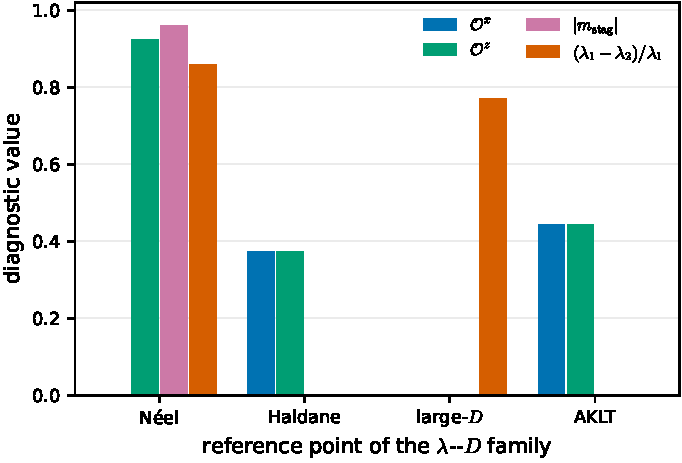
\includegraphics[width=0.78\textwidth]{figures/lambdaD-phase-points.pdf}
\caption{Ground-state diagnostics of the spin-1 $\lambda$--$D$ chain
\cref{eq:num-lambdaD} at its four reference points, at the largest bond
dimension computed ($\chi=48$). The N\'eel point ($\Delta=2.5$, $D=0$) has
$\mathcal{O}^x = 10^{-23}$ but $\mathcal{O}^z = 0.9255$ and staggered
magnetisation $0.9603$; the Haldane point ($\Delta=1$, $D=0$) has
$\mathcal{O}^x = \mathcal{O}^z = 0.3743$ and an entanglement doublet that is
exactly degenerate at the resolution of the calculation; the large-$D$ point
($\Delta=1$, $D=2.5$) has both string orders zero and a split spectrum; the
AKLT point ($\Delta=1$, $D=0$, $K=\tfrac13$) reproduces its closed forms
$\mathcal{O}^x=\mathcal{O}^z=4/9$, $e=-2/3$ and $S=\log 2$ to the printed
digits. The figure makes the operational point of the whole programme:
$\mathcal{O}^z$ is \emph{large} in the N\'eel phase and therefore does not
distinguish it from Haldane, whereas $\mathcal{O}^x$ does.}
\label{fig:lambdaD-phase-points}
\end{figure}

\begin{figure}[t]
\centering
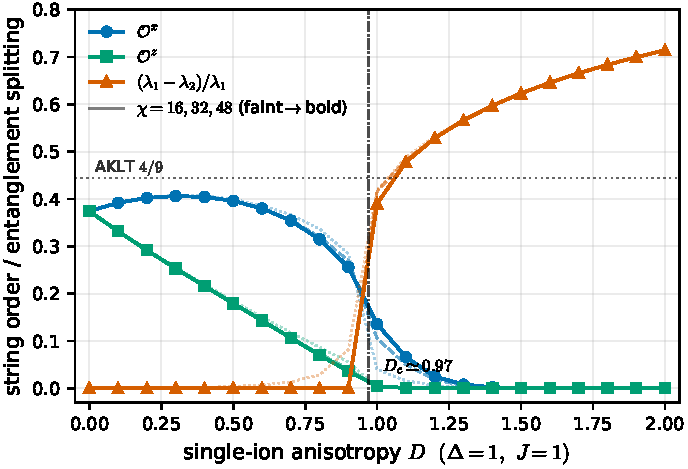
\includegraphics[width=0.78\textwidth]{figures/lambdaD-D-sweep.pdf}
\caption{The Haldane-to-large-$D$ sweep at $\Delta=1$: string order
parameters and the relative splitting of the leading entanglement doublet,
each recorded at $\chi=16,32,48$ (faint to bold) so that the bond-dimension
drift is visible. This is the rigidity dichotomy in one panel. The bulk
coefficient $\mathcal{O}^x$ \emph{drifts continuously} from its Heisenberg
value $0.374$ down through $0.256$ as $D$ approaches the transition, while the
entanglement doublet stays degenerate to below $5\times10^{-12}$ over the
whole Haldane side and then jumps by an $O(1)$ amount --- from
$4\times10^{-12}$ at $D=0.9$ to $0.39$ at $D=1.0$, eleven orders of magnitude
in one step of the sweep --- bracketing the literature value
$D_c\simeq0.97$. A quantised discrete datum survives exactly where a
continuous one is already sliding.}
\label{fig:lambdaD-D-sweep}
\end{figure}

\begin{figure}[t]
\centering
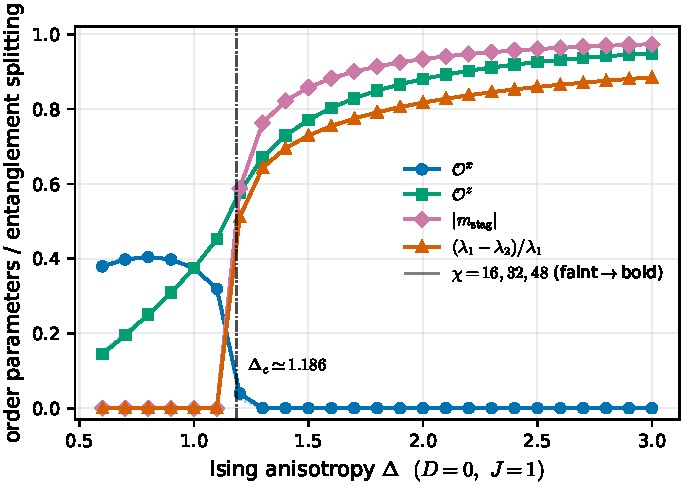
\includegraphics[width=0.78\textwidth]{figures/lambdaD-delta-sweep.pdf}
\caption{The Haldane-to-N\'eel sweep at $D=0$, on a two-site unit cell so that
the symmetry-broken state is representable. The staggered magnetisation and
the entanglement splitting switch on together between $\Delta=1.1$ (both below
$10^{-13}$) and $\Delta=1.2$ ($0.587$ and $0.511$ respectively), bracketing the
literature value $\Delta_c\simeq1.186$. $\mathcal{O}^x$ collapses across the
same window ($0.319 \to 0.039 \to 1.5\times10^{-4}$ at
$\Delta=1.1,1.2,1.3$), whereas $\mathcal{O}^z$ \emph{grows} straight through
the transition ($0.452 \to 0.577 \to 0.671$) and is therefore useless as a
phase discriminator here --- the point already made statically in
\cref{fig:lambdaD-phase-points}.}
\label{fig:lambdaD-delta-sweep}
\end{figure}

\Cref{fig:lambdaD-phase-points} fixes the four reference points and their
calibration. \Cref{fig:lambdaD-D-sweep,fig:lambdaD-delta-sweep} follow the
diagnostics across the two transitions. The headline is the one recorded in
\cref{sec:spt}: across the Haldane boundary the entanglement doublet is exact
until it is not, jumping by an $O(1)$ amount at a transition that a continuous
bulk order parameter merely drifts through. The critical points bracketed by
the jumps agree with the literature values $D_c\simeq0.97$ and
$\Delta_c\simeq1.186$.

Three controls support the reading. The AKLT point is a zero-parameter test of
nine closed-form numbers at once --- energy density, correlation length,
entropy, both string orders, exactly two Schmidt values each $1/\sqrt2$, a
vanishing doublet splitting, vanishing staggered order, and the exact
correlator $\langle S^z_1S^z_{1+r}\rangle = \tfrac43(-\tfrac13)^r$ out to
$r=8$ --- and it passes to the printed digits; in the charge-graded backend
the two Schmidt states are additionally found to sit in $S^z$ sectors exactly
one unit apart, which is the edge doublet read straight off the charge labels.
The Haldane doublet splitting reaches $9\times10^{-14}$ at the largest bond
dimension and stays below $5\times10^{-12}$ across the entire Haldane side of
the sweep, so the degeneracy is exact at the resolution of the calculation
rather than merely small. And the N\'eel point is deliberately run once more on
a \emph{one-site} unit cell, which cannot represent a symmetry-broken state and
is expected \emph{not} to converge: that failure is itself the evidence that
the breaking is physical, and the row is kept in the record with its
diagnostics visibly nonsensical.

Two caveats belong with these figures. The bond dimensions available on the
hardware used, $\chi\in\{16,32,48\}$, are not enough to resolve a critical
point: near a transition the correlation length and the string order are
$\chi$-limited, which is why every point is recorded at all three bond
dimensions rather than at the best one. And the reported correlation length is
the maximum over \emph{all} transfer-matrix channels, which need not be the
longitudinal channel that a $\langle S^zS^z\rangle$ fit sees; in the large-$D$
phase the two differ by more than a factor of two because the longest channel
there is transverse.

\provenance{--- (calibration and phase data for \cref{sec:spt})}
{--- (numerical record, no theorem asserted)}
{\texttt{numerics/\allowbreak{}results/\allowbreak{}lambdaD-\allowbreak{}phase-\allowbreak{}points.json} (17 rows),
 \texttt{lambdaD-\allowbreak{}D-\allowbreak{}sweep.json} (63 rows),
 \texttt{lambdaD-\allowbreak{}delta-\allowbreak{}sweep.json} (75 rows); produced by
 \texttt{numerics/\allowbreak{}scripts/\allowbreak{}run\_\allowbreak{}lambdaD\_\allowbreak{}phases.jl}; gated by
 \texttt{numerics/\allowbreak{}test/\allowbreak{}test\_\allowbreak{}lambdaD\_\allowbreak{}groundstate.jl}}
{bd lane \texttt{tns-f5r} wave 1}

\subsection{The \texorpdfstring{$\lambda$--$D$}{lambda-D} kink: dispersion and memory coefficient}\label{sec:numerics-kink}

The second production programme puts a kink of the N\'eel phase in motion and
measures what a magnon-like wavepacket does to it, in the non-integrable
setting of \cref{eq:num-lambdaD}. It runs at $\Delta=2.5$, $D=0$, $J=1$, deep
in the N\'eel phase, where the measured staggered tail density is
\begin{equation}
  s \;=\; m_{\text{stag}} \;=\; 0.960340 ,
  \label{eq:num-s}
\end{equation}
an ordinary number rather than a half-integer. This matters for reading the
prediction: the memory law of \cref{sec:memory-quantization} predicts the
coefficient $2s$, and $2s = 1.920680$ here.

\begin{figure}[t]
\centering
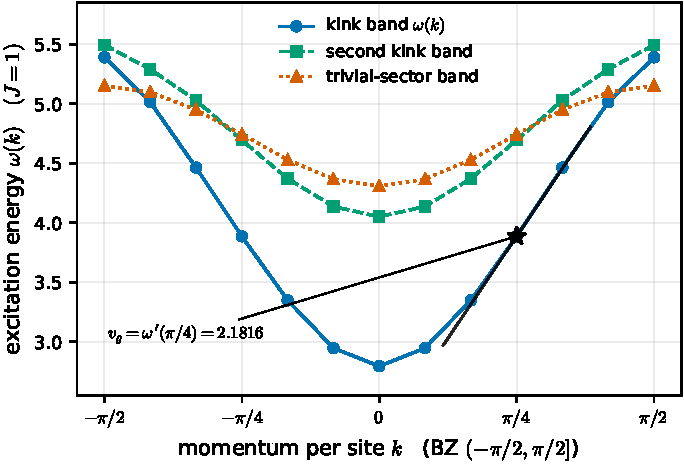
\includegraphics[width=0.78\textwidth]{figures/lambdaD-kink-dispersion.pdf}
\caption{Kink dispersion in the topological sector of the $\lambda$--$D$ chain
at $\Delta=2.5$, $D=0$, obtained from a quasiparticle excitation ansatz with
the two broken N\'eel vacua as left and right boundary conditions. Momentum is
per site, so $\omega(k)=\omega(k+\pi)$ and the zone is $(-\pi/2,\pi/2]$. The
kink band is gapped ($\Delta E = 2.7947$) with bandwidth $2.5957$ and is
cleanly separated from the second kink band and from the trivial-sector band
over the whole zone --- the separation that makes a single-band wavepacket
meaningful. The straight line is the tangent at the working momentum
$k_0=\pi/4$, giving $\omega(k_0)=3.886051$ and the group velocity
$v_g=2.181628$ against which the transport runs are calibrated. Three bond
dimensions ($\chi=16,24,32$) agree to nine significant figures, so only the
largest is drawn.}
\label{fig:lambdaD-kink-dispersion}
\end{figure}

\begin{figure}[t]
\centering
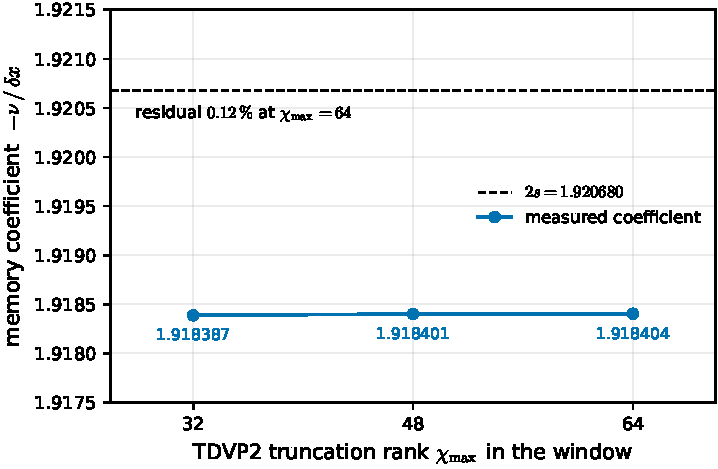
\includegraphics[width=0.78\textwidth]{figures/lambdaD-kink-memory-convergence.pdf}
\caption{Truncation-rank convergence of the measured memory coefficient
$-\delta x/\nu$ for the $\lambda$--$D$ kink transport at $L=48$, against the
predicted $2s=1.920680$ of \cref{eq:num-s}. Raising the two-site truncation
rank inside the evolution window from $\chi_{\max}=32$ to $64$ moves the
coefficient by $3.1\times10^{-6}$, from $1.9183874$ to $1.9184040$: the number
is converged in the truncation. The residual gap to $2s$ is $0.12$ per cent
and is a property of the finite window and readout geometry, not of the
truncation. The supporting quality gates are a norm drift of
$1.4\times10^{-6}$ and an energy drift of $2.6\times10^{-4}$ over the readout
interval.}
\label{fig:lambdaD-kink-memory-convergence}
\end{figure}

Two points about \cref{fig:lambdaD-kink-dispersion} matter for how the
transport numbers should be read. The band is \emph{computed}, not fitted: it
comes from a variational quasiparticle solve at each momentum, and the group
velocity is a central difference over three such solves. It is therefore fixed
\emph{before} any dynamics, and the measured wavepacket velocity is tested
against it rather than fitted to it. The wavepacket itself is built from the
variationally optimised excitation tensor at the working momentum; an
undressed step from one vacuum to the other is kept only as a deliberately bad
control, and it is bad by a wide margin --- its energy exceeds the band by
$9.8$, against a gate of $1.0$, where the dressed packet sits within
$3.7\times10^{-3}$ of $\omega(k_0)$.

\Cref{fig:lambdaD-kink-memory-convergence} then establishes that the memory
coefficient extracted from the transport is converged in the one parameter
that could plausibly have been controlling it. At the largest rank the run
measures a mean escaped charge $\nu=-16.372936$ and, with the $s$-free
centroid estimator, a wall displacement of $\delta x = 8.534665$ sites, giving
\begin{equation}
  -\frac{\nu}{\delta x} \;=\; 1.918404
  \qquad\text{against}\qquad 2s = 1.920680 ,
  \label{eq:num-coefficient}
\end{equation}
a deviation of $0.12$ per cent. Because the estimator on the left does not
contain $s$, this is a measurement of the coefficient and not an identity. The
measured propagation velocity in the window, $2.1343$, sits $2.2$ per cent
below the band value $2.1816$ of \cref{fig:lambdaD-kink-dispersion}, which is
the size one expects from a packet of finite width sampling the band
curvature.

The integer structure behind the law is certified separately, on the same
state and the same window. The windowed charge has
$|\langle e^{2\pi i\Qhat_W}\rangle| = 0.99995$ with a phase defect of
$5\times10^{-15}$ --- its spectrum lies in one coset of $\mathbb{Z}$, so every
escaped-charge outcome is an integer --- while the wall coordinate has
$|\langle e^{2\pi i\wallX_W}\rangle| = 0.438$, comfortably below one, as
it must be since $2s\notin\mathbb{Z}$. Displacing the window charge law's
weight to $1/(2s)$ turns the inversion into an aliased signed measure with
genuinely negative entries, and the test asserts that it does. The wall
displacement is not quantised; the charge is.

This is evidence for the memory law of \cref{sec:memory-quantization} in a
model with no integrability to lean on, and it is not a proof of anything. Two
limitations are stated in the source and should be stated here. First, the
protocol measures the \emph{bookkeeping} half of the memory statement: nothing
scatters off the wall in this run, so the displacement is ballistic transport
of a single packet, and a memory in the sense of a transient perturbation
leaving a permanent offset would require a second excitation inside the window
and is not attempted. Second, what is recorded is the exact single-time law of
the windowed charge at each sample; that coincides with the ordered two-point
measurement law of the theory only under the additional hypothesis named
there, which is carried in the record as an assumption and not as a result.

\provenance{--- (evidence for the memory law of \cref{sec:memory-quantization};
 no claim promoted)}
{--- (numerical record)}
{\texttt{numerics/\allowbreak{}results/\allowbreak{}lambdaD-\allowbreak{}kink-\allowbreak{}dispersion.json} (3 rows),
 \texttt{lambdaD-\allowbreak{}kink-\allowbreak{}memory-\allowbreak{}convergence.json} (3 rows); produced by
 \texttt{numerics/\allowbreak{}scripts/\allowbreak{}run\_\allowbreak{}lambdaD\_\allowbreak{}memory.jl}; gated by
 \texttt{numerics/\allowbreak{}test/\allowbreak{}test\_\allowbreak{}lambdaD\_\allowbreak{}memory.jl}}
{bd lane \texttt{tns-f5r} wave 2;
 \texttt{theory/\allowbreak{}lanes/\allowbreak{}blitz-\allowbreak{}2026-\allowbreak{}08-\allowbreak{}29/\allowbreak{}wave2-\allowbreak{}repair/\allowbreak{}SUMMARY.md}}

\subsection{The \texorpdfstring{$\lambda$--$D$}{lambda-D} edge: the memory contrast between phases}\label{sec:numerics-edge}

The third $\lambda$--$D$ experiment is the static counterpart of the
transport run. A ground state is prepared with boundary fields
$h_L=+\tfrac12$ and $h_R=-\tfrac12$ on a chain of $L=40$ sites, the left field
is switched off at $t=0$, and the magnetisation of the left half is followed.
The Haldane phase has a protected edge spin-$\tfrac12$ and should hold its
polarisation; the large-$D$ phase has no edge mode and should not acquire one.

\begin{figure}[t]
\centering
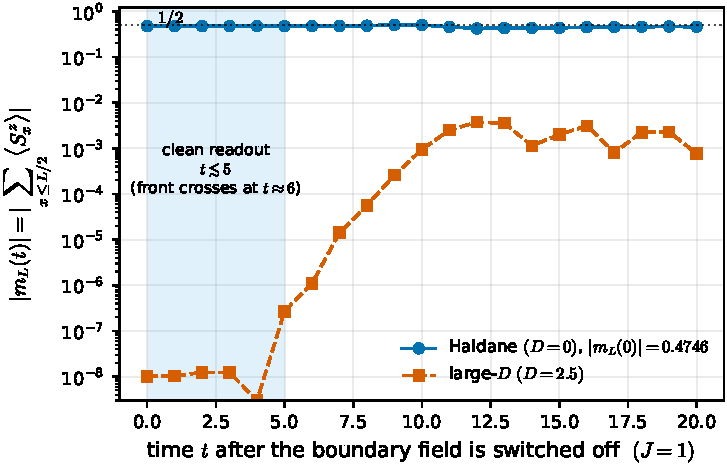
\includegraphics[width=0.78\textwidth]{figures/lambdaD-edge-memory.pdf}
\caption{Edge memory after the left boundary field is switched off, on a
logarithmic scale, for the Haldane point ($D=0$) and the trivial large-$D$
point ($D=2.5$) of the same Hamiltonian family, at $L=40$. The Haldane chain
carries $|m_L(0)| = 0.4746$, close to the half unit expected of a protected
edge spin-$\tfrac12$, and holds it; the large-$D$ chain never exceeds
$3.7\times10^{-3}$, a contrast of a factor $127$. The shaded band is the only
honest readout window: a bulk magnon front of speed $v\approx2.5$ reaches the
window edge at $t\approx6$, after which $|m_L|$ overshoots $\tfrac12$ because
bulk charge is crossing the window, not because the edge is decaying. Data
outside the band, including the record's $t=20$ "retention" field, is
front-contaminated (see \cref{sec:numerics-honesty}).}
\label{fig:lambdaD-edge-memory}
\end{figure}

\begin{figure}[t]
\centering
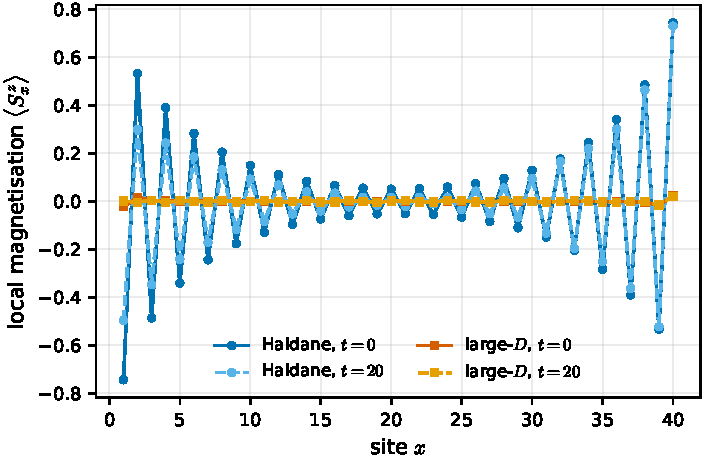
\includegraphics[width=0.78\textwidth]{figures/lambdaD-edge-profile.pdf}
\caption{Local magnetisation profiles for the same two runs, at preparation
and at the end of the evolution. The Haldane profile shows the staggered,
exponentially decaying edge moment characteristic of a fractionalised
boundary spin, essentially unchanged by the evolution; the large-$D$ profile
is flat at the resolution of the plot in both phases of the protocol. The
right-hand rise in the Haldane curves is the \emph{other} edge, which is
pinned by a permanent field for the whole run.}
\label{fig:lambdaD-edge-profile}
\end{figure}

\Cref{fig:lambdaD-edge-memory,fig:lambdaD-edge-profile} show the contrast.
Read together with \cref{eq:num-edge-fss}, which extrapolates the edge moment
to $\tfrac12$ as $L\to\infty$ with a decay length matching the spin-1
Heisenberg correlation length, they are the numerical face of the rigidity
statement of \cref{sec:spt}: a discrete, quantised boundary datum that a
trivial phase simply does not have.

Four caveats travel with these runs and are recorded in the data file. The
finite-chain Haldane retention is exact only up to the edge--edge splitting
time, which grows like $e^{L/\xi}$. The right edge is pinned throughout. The
choice $h_R=-h_L$ places both phases in the total-$S^z$ zero sector, so that
$m_L$ is a genuine measurement rather than half of a conserved total --- with
$h_R=+h_L$ the diagnostic would have been a symmetry artefact. And the
\emph{relative} retention of the large-$D$ run is a ratio of numerical zeros
and is meaningless; the absolute numbers are the ones to quote.

\provenance{--- (evidence for the boundary rigidity of \cref{sec:spt})}
{--- (numerical record)}
{\texttt{numerics/\allowbreak{}results/\allowbreak{}lambdaD-\allowbreak{}edge-\allowbreak{}memory.json} (2 rows); produced by
 \texttt{numerics/\allowbreak{}scripts/\allowbreak{}run\_\allowbreak{}lambdaD\_\allowbreak{}memory.jl}; gated by
 \texttt{numerics/\allowbreak{}test/\allowbreak{}test\_\allowbreak{}lambdaD\_\allowbreak{}memory.jl}}
{bd lane \texttt{tns-f5r} wave 2; open defect \texttt{tns-nkf}}

\subsection{The spin-\texorpdfstring{$s$}{s} falsifier battery}\label{sec:numerics-bc}

The conjecture at issue is the one discussed in \cref{sec:triangle-status}:
that the soft phase slope and the memory quantum are the same asymptotic
charge datum $|q_{\text{hard}}|/s$. At $s=\tfrac12$ both are $2$, which is
exactly the sort of coincidence that deserves to be attacked. The falsifier
was stated in advance: if the spin-1 phase slope is not $1$, the coincidence
is numerology and the conjecture must be dropped.

The analytic input is a contact solution of the spin-$S$ two-magnon problem,
obtained without any integrability assumption by keeping the free extension
$\Psi$ \emph{unsymmetrised} and matching on the physical chamber. Writing
$K=k_1+k_2$, $q=(k_1-k_2)/2$, $c=\cos(K/2)$ and
\begin{equation}
  n \;:=\; 2Sc\cos q - e^{iq}\bigl[(2S-1)c + \cos q\bigr],
  \label{eq:num-contact}
\end{equation}
the ratio is $S_{12} = n/(-\bar n)$, manifestly of unit modulus, and the soft
expansion gives
\begin{equation}
  \frac{\partial\delta}{\partial k_s}\Big|_{k_s=0} \;=\; \frac{1}{S},
  \label{eq:num-slope}
\end{equation}
with all hard-momentum dependence cancelling. At $S=\tfrac12$ the $(2S-1)c$
term vanishes and the expression collapses to the frozen $s=\tfrac12$ oracle
formula, checked to $10^{-12}$.

\begin{figure}[t]
\centering
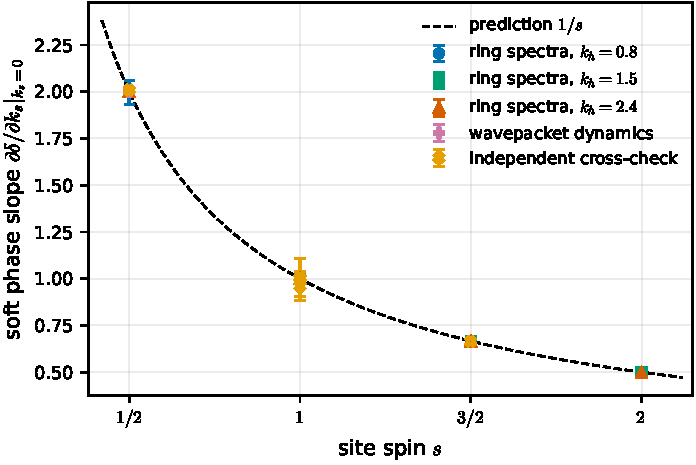
\includegraphics[width=0.78\textwidth]{figures/bc-soft-slope.pdf}
\caption{Measured soft phase slope $\partial\delta/\partial k_s|_0$ against
site spin, versus the predicted $1/s$. The ring points are \emph{ansatz-free}:
exact total-momentum-block spectra of the two-magnon sector are inverted
through $E=\omega(k_1)+\omega(k_2)$ and the Bethe--Yang quantisation
$Nk_s = 2\pi n_s + \delta$, extrapolated over
$N\in\{60,90,120,180,240,360,480\}$; no wavefunction ansatz and no $S$-matrix
enters. Independent wavepacket dynamics and an independent cross-check by
different methods are overlaid. Every one of the twelve ring determinations
lies within $0.003$ of $1/s$: $1.9979$--$2.0010$ at $s=\tfrac12$,
$0.9972$--$0.9995$ at $s=1$, $0.6645$--$0.6654$ at $s=\tfrac32$, and
$0.4978$--$0.4989$ at $s=2$. The prediction $2$ for every spin --- the outcome
that would have killed the conjecture --- is excluded by many standard
deviations at $s\geq1$.}
\label{fig:bc-soft-slope}
\end{figure}

\begin{figure}[t]
\centering
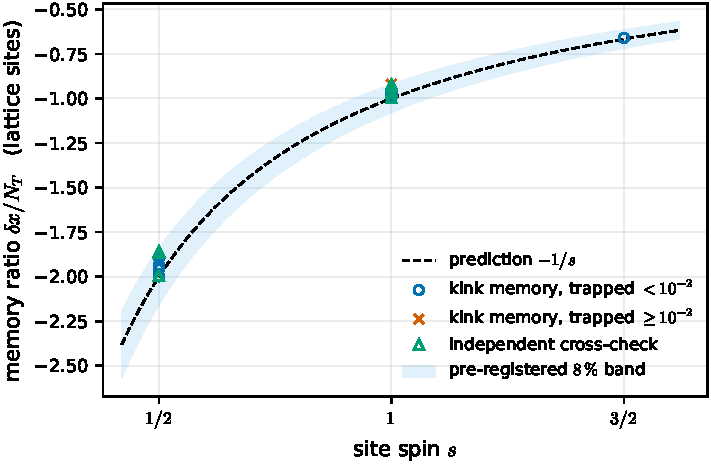
\includegraphics[width=0.78\textwidth]{figures/bc-memory-ratio.pdf}
\caption{The memory half of the same battery: measured ratio
$\delta x/N_T$ from spin-$s$ kink-transport runs, against the predicted
$-1/s$ and the pre-registered eight-per-cent decision band fixed before the
first run. Circles are runs whose trapped weight is below $10^{-2}$, so that
the asymptotic condition behind the law is actually met; crosses are the runs
where it is not. The nine spin-1 grid points average $-0.97996$, and the eight
of them with small trapped weight average $-0.98755$, within $1.3$ per cent of
$-1$; four spin-$\tfrac12$ controls on the same code path average $-1.97817$;
the single spin-$\tfrac32$ point gives $-0.66015$ against $-0.66667$ and is
the sharpest of all because it has only partial transmission ($T=0.383$), so
the ratio is not near-saturated.}
\label{fig:bc-memory-ratio}
\end{figure}

\Cref{fig:bc-soft-slope,fig:bc-memory-ratio} show both halves. Three
independent routes agree on the slope --- an exact-eigenvector residual test
at Bethe--Yang momenta, the ansatz-free ring extraction, and wavepacket
dynamics --- and across all $84$ ring rows the extracted phase agrees with the
analytic spin-$S$ expression to $8\times10^{-13}$. The memory ratio is
supported by size convergence (three chain lengths agreeing to five decimals),
by sharp-versus-dressed initial walls agreeing to $0.5$ per cent, and by the
basis-enlargement check quoted in \cref{sec:numerics-code}.

Two pieces of restraint belong with these numbers. The independent cross-check
records four of its fourteen memory runs as \emph{inconclusive} --- all at the
lower working momentum, where the packet is too broad in momentum for the
asymptotic reading and the two linear estimators bracket the prediction with a
spread of $0.17$ --- and those runs are kept in the published record with the
diagnosis attached rather than dropped. And the largest spin was reached only
at a reduced chain length: the corresponding sector needs of order twenty-four
gigabytes at the production size, and an attempt there was killed by the
operating system, so the $s=\tfrac32$ point is a single run on a shorter chain
and is the weakest of the battery.

The verdict is that the conjecture \emph{survived} both falsifiers. It remains
\statusConjecture. What the runs test sharply is the $1/s$ factor, since $s$
is varied over $\{\tfrac12,1,\tfrac32,2\}$; what they did not test is the
$|q_{\text{hard}}|$ factor, because every leg in every run carries unit
charge. That gap was later attacked directly: a three-magnon exact
diagonalisation at $N=100$ and $s=\tfrac12$, in which the hard leg is a
charge-two bound state, measured a slope of
\begin{equation}
  4.070 \pm 0.090 \qquad\text{against}\qquad |q_{\text{hard}}|/s = 4 ,
  \label{eq:num-charge2}
\end{equation}
inside a pre-registered absolute window of $0.35$, with a dense-sector oracle
running green and a deliberate mutation of the hopping running red. This too
is finite-packet evidence at a single volume and a single packet width: there
is no size or width extrapolation, and no charge-two kink-memory experiment
exists. The conjecture stays where it was.

\provenance{Bc}
{--- (conjecture; the slope half at unit charge is a separate proved row, see
 \cref{sec:two-magnon})}
{\texttt{numerics/\allowbreak{}results/\allowbreak{}spin1-\allowbreak{}bc-\allowbreak{}falsifier.json} ($84$ ring, $16$ dynamical,
 $22$ memory rows); \texttt{spin1-\allowbreak{}bc-\allowbreak{}crosscheck.json};
 \texttt{numerics/\allowbreak{}scripts/\allowbreak{}run\_\allowbreak{}spin1\_\allowbreak{}bc\_\allowbreak{}falsifier.jl},
 \texttt{run\_\allowbreak{}spin1\_\allowbreak{}bc\_\allowbreak{}crosscheck.jl}; decision tests in
 \texttt{numerics/\allowbreak{}test/\allowbreak{}test\_\allowbreak{}spins\_\allowbreak{}twomagnon.jl},
 \texttt{test\_\allowbreak{}spins\_\allowbreak{}memory.jl}, \texttt{test\_\allowbreak{}spin1\_\allowbreak{}twomagnon.jl},
 \texttt{test\_\allowbreak{}spin1\_\allowbreak{}memory.jl}}
{bd lane \texttt{tns-8e9}; charge-two lane
 \texttt{theory/\allowbreak{}lanes/\allowbreak{}blitz-\allowbreak{}2026-\allowbreak{}08-\allowbreak{}29/\allowbreak{}bc-\allowbreak{}charge2/\allowbreak{}}}

\subsection{The ferromagnetic two-magnon displacement scan}\label{sec:numerics-fm}

The soft theorem of \cref{sec:two-magnon} is derived algebraically. The
displacement scan tests it dynamically, and the test is genuinely independent:
the code never writes down a Bethe wavefunction. It enumerates down-spin
pairs, assembles the two-magnon Hamiltonian from the model directly, launches
two Gaussian packets in the incoming configuration --- hard behind soft, so
that the hard magnon overtakes --- and measures how far each outgoing packet
has been displaced relative to free propagation. By \cref{eq:num-wigner} those
displacements \emph{are} the momentum derivatives of the scattering phase, so
a sign error, a wrong branch or a swapped channel convention would show up
immediately.

\begin{figure}[t]
\centering
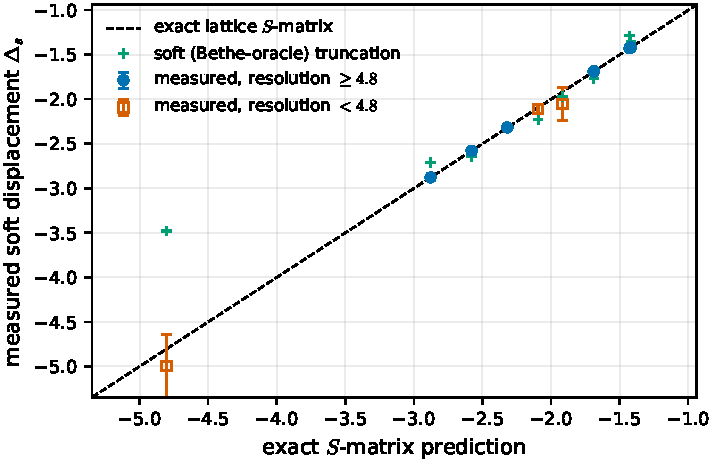
\includegraphics[width=0.78\textwidth]{figures/fm-displacement-soft.pdf}
\caption{Measured soft-magnon displacement $\Delta_s$ against the exact
lattice $S$-matrix prediction, for ten kinematic points of the spin-$\tfrac12$
isotropic Heisenberg ferromagnet; the dashed line is equality. Each point is
Richardson-extrapolated in $1/\sigma_x^2$ from packet widths
$\sigma_x\in\{8,11,14\}$, with the error bar the spread over all width pairs.
Every point agrees with the exact $S$-matrix inside its own error bar; where
the wavepacket geometry is well resolved the deviation is $3\times10^{-6}$ to
$5\times10^{-4}$, i.e.\ four to six significant digits of a scattering-phase
derivative recovered from real-time dynamics alone. The crosses are the soft
truncation of the theorem, which deviates visibly and by design --- most
dramatically at the leftmost point, where the soft hierarchy is deliberately
violated and the dynamics side with the exact $S$-matrix, confirming the
theorem's stated validity domain rather than refuting it.}
\label{fig:fm-displacement-soft}
\end{figure}

\begin{figure}[t]
\centering
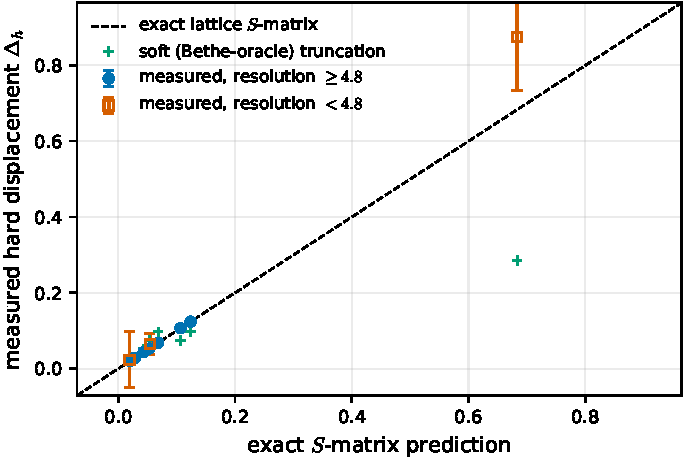
\includegraphics[width=0.78\textwidth]{figures/fm-displacement-hard.pdf}
\caption{The same comparison for the hard-magnon displacement $\Delta_h$.
It is positive in all ten runs and one to two orders of magnitude smaller than
$\Delta_s$ --- the classical hard-sphere pattern, with the overtaken particle
recoiling backwards by the contact length and the overtaking one jumping
forwards. This is the structural content of the soft theorem made visible: the
leading term of the phase carries no hard-momentum dependence and therefore
cannot displace the hard packet at all, so $\Delta_h$ is quadratic in the soft
momentum.}
\label{fig:fm-displacement-hard}
\end{figure}

\Cref{fig:fm-displacement-soft,fig:fm-displacement-hard} show the two
displacements. Beyond the pointwise agreement, the coefficients of the soft
expansion can be read off the dynamics with no $S$-matrix input at all, by
combining runs at $+k_s$ and $-k_s$: the antisymmetric combination isolates
the first hard invariant and the symmetric one the leading scattering length.
Extrapolating the two available soft momenta at fixed hard momentum gives
$2.147178$ for the former, against $2.147197$ from the exact lattice
$S$-matrix and $2\cot(k_h/2) = 2.146852$ from the theorem, and the latter
converges to $2$ within $0.2$ per cent. \textbf{The leading, hard-data
independent scattering length $2$ is a directly measured lattice
displacement}, not an artefact of an ansatz.

The one place where the dynamical method is strictly weaker than the algebra
is kinematic rather than analytic: as the hard momentum approaches $\pi$ its
group velocity vanishes, the incoming condition becomes almost unsatisfiable,
and the collision takes $O(10^3)$ time units. The accuracy is controlled by a
single dimensionless resolution --- final separation over combined final
packet width --- and, because dispersive spreading grows with the propagation
time, pushing the packets further apart does not improve it; only fatter
packets or a faster relative velocity do, at cost cubic in the packet width.

The related claim row \texttt{N1}, that excitation-ansatz magnon amplitudes
reproduce the Bethe $S$-matrix in the soft limit, has \emph{not} been run and
remains \statusConjecture\ with no supporting data.

\provenance{N1 (not run); supporting data for the two-magnon soft expansion of
 \cref{sec:two-magnon}}
{--- (numerical record)}
{\texttt{numerics/\allowbreak{}results/\allowbreak{}fm-\allowbreak{}displacement-\allowbreak{}scan.json} ($10$ summary rows over
 $30$ evolutions); produced by \texttt{numerics/\allowbreak{}src/\allowbreak{}fm\_\allowbreak{}twomagnon.jl};
 gated by \texttt{numerics/\allowbreak{}test/\allowbreak{}test\_\allowbreak{}fm\_\allowbreak{}twomagnon.jl}}
{\texttt{numerics/\allowbreak{}docs/\allowbreak{}fm-\allowbreak{}twomagnon-\allowbreak{}notes.md}}

\subsection{The XXZ kink-memory scan}\label{sec:numerics-xxz}

The last family is the original spin-$\tfrac12$ memory experiment: a magnon
wavepacket sent at a kink in the easy-axis chain \cref{eq:num-xxz}, with the
displacement of the kink measured before and after.

The bookkeeping argument is worth stating because it is what the data
confirms. Before the collision the state is a kink at $X$ plus one extra down
spin in the up region. After full transmission the magnon is an \emph{up}
bubble in the down region, at the same total $S^z$. The wall must absorb the
difference, and it can only do so by moving two sites. Hence a transmitted
magnon displaces the kink by exactly $-2$ sites, a reflected one by zero, and
\begin{equation}
  \delta x \;=\; -2\,T ,
  \label{eq:num-dx2T}
\end{equation}
so the memory is quantised and the whole of its magnitude sits in the
transmission probability. On the lattice the collective coordinate can only
shift in units of two sites and the continuous observable is the \emph{weight}
$T$, not the displacement.

\begin{figure}[t]
\centering
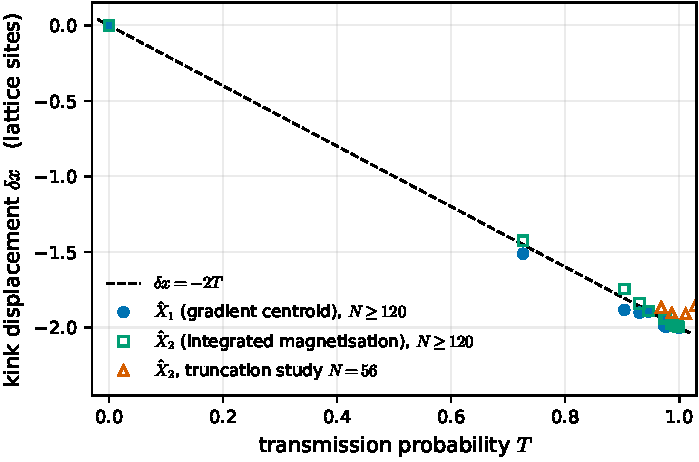
\includegraphics[width=0.78\textwidth]{figures/xxz-memory-dx-vs-T.pdf}
\caption{Kink displacement against transmission probability for the
spin-$\tfrac12$ XXZ memory scan, with the prediction $\delta x = -2T$ of
\cref{eq:num-dx2T} as the dashed line. Production runs at $N\geq120$ are shown
for both linear estimators; the $N=56$ points are the truncation study, whose
geometry carries much larger systematics. Over the whole scan
$|\delta x_1 + 2T| \leq 0.075$, and at the cleanest geometries --- those with
trapped weight below $10^{-6}$ --- the residual is $0.004$ sites. Three chain
lengths $N=120,160,200$ reproduce the same numbers to six significant figures,
and an Ising control with the exchange switched off returns
$T=0$, $R=1$ and $\delta x=0$ exactly.}
\label{fig:xxz-memory-dx-vs-T}
\end{figure}

\begin{figure}[t]
\centering
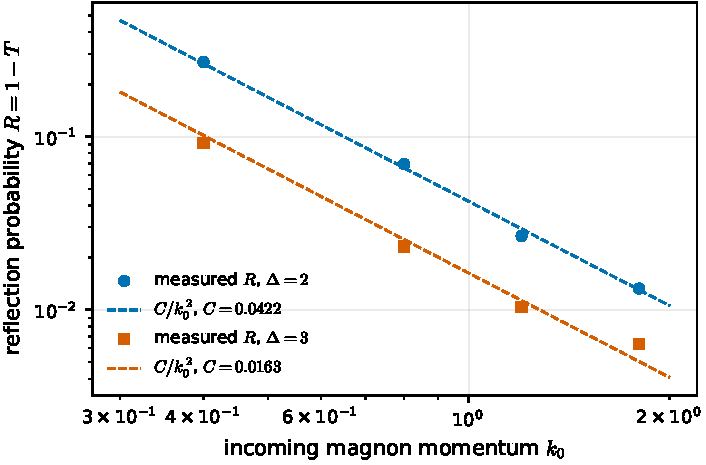
\includegraphics[width=0.78\textwidth]{figures/xxz-reflection-threshold.pdf}
\caption{Reflection probability against incoming magnon momentum, on
logarithmic axes, at two anisotropies, with fitted curves $C(\Delta)/k_0^2$.
The measured $R$ follows the one-dimensional low-energy threshold law with
$C(2)\approx0.042$ and $C(3)\approx0.016$, so $T\to0$ and, by
\cref{eq:num-dx2T}, $\delta x\to0$ as $k_0\to0$: \emph{a soft magnon leaves no
memory}. This is the model's Adler-type zero, and it is the qualitative
content of the soft theorem seen from the memory side. In the same regime
$C(\Delta)$ falls like $\Delta^{-2}$, so the kink becomes \emph{more}
transparent, and the memory closer to its quantum, the deeper the easy axis.}
\label{fig:xxz-reflection-threshold}
\end{figure}

\Cref{fig:xxz-memory-dx-vs-T} is the quantitative statement and
\cref{fig:xxz-reflection-threshold} the physical one. A refuted prior
expectation belongs here too, since it was recorded before the runs: it was
predicted that at large anisotropy the kink would be an opaque barrier. It is
not. Transmission tends to \emph{one} as $\Delta\to\infty$. The mechanism is
visible in the domain-wall algebra --- the elementary exchange move takes a
magnon adjacent to the wall on the up side directly into a bubble on the down
side, displacing the wall by two, so transmission is a first-order,
energy-conserving process inside the retained manifold, while the merge
channel that produces reflection is off-resonant by one magnon gap. The
easy-axis kink is nearly transparent to magnons, and the more so the deeper
the easy axis. This is the numerical face of the decoupling statement of
\cref{sec:kink-model}: the magnon couples to the wall's collective coordinate
and to nothing else.

This is the evidence behind claim row \texttt{N2}, and it is held at
\statusSketch. The row says exactly what it is: an empirical scan matching the
conditional memory expectation at the recorded precision, $\delta x \approx
-2T$ to within $0.004$ sites. It is numerical evidence, not a theorem, and it
does not promote the conditional theorem it agrees with.

\provenance{N2 \statusSketch}
{--- (empirical scan only; the theorem it agrees with is conditional and lives
 in \cref{sec:memory-quantization})}
{\texttt{numerics/\allowbreak{}results/\allowbreak{}memory-\allowbreak{}scan-\allowbreak{}1.json} ($21$ runs); produced by
 \texttt{numerics/\allowbreak{}scripts/\allowbreak{}run\_\allowbreak{}memory\_\allowbreak{}scan.jl} over
 \texttt{numerics/\allowbreak{}src/\allowbreak{}xxz\_\allowbreak{}sector.jl}, \texttt{xxz\_\allowbreak{}dynamics.jl},
 \texttt{memory\_\allowbreak{}experiment.jl}; gated by
 \texttt{numerics/\allowbreak{}test/\allowbreak{}test\_\allowbreak{}xxz\_\allowbreak{}sector.jl},
 \texttt{test\_\allowbreak{}xxz\_\allowbreak{}dynamics.jl}, \texttt{test\_\allowbreak{}memory\_\allowbreak{}experiment.jl}}
{\texttt{numerics/\allowbreak{}docs/\allowbreak{}kink-\allowbreak{}sector-\allowbreak{}notes.md}}

\subsection{Honesty: defects, quarantine, and what none of this proves}\label{sec:numerics-honesty}

\subsubsection*{A quarantined record}

The $\lambda$--$D$ transport production stage produced one record that is
\emph{not} a result and is not plotted anywhere in this section. The file
\texttt{numerics/\allowbreak{}results/\allowbreak{}lambdaD-\allowbreak{}kink-\allowbreak{}memory.FAILED-\allowbreak{}NaN.json} is quarantined
under a name that says so.

What happened is this. The stage ran two rows at $L=72$, one for each initial
dressing of the kink. The evolution itself was clean in both: energies, norms
and position time series are finite throughout, out to $t=14$. The first row,
with a quasiparticle-dressed initial kink, completed normally and reported a
coefficient of $1.9131$ against $2s=1.920680$. The second row, with a
deliberately undressed sharp kink, has \emph{every} analysis output
non-finite: measured velocity, all three displacement estimators, the mean
escaped charge and the coefficient.

The mechanism is visible in the record and is worth stating precisely, because
it is more specific than "the fit broke". The readout interval is selected by
requiring both that the wall be padded from the window edges and that the
measured edge leakage stay below a fixed tolerance of $10^{-3}$. For the sharp
preparation the leakage starts at $5\times10^{-3}$ --- already five times the
tolerance at $t=0$ --- and grows monotonically to $0.159$. No sample ever
qualifies, the recorded readout index range is empty, and the analysis
correctly declines to compute a displacement outside the region where its
definition applies, returning non-finite values instead. That branch is doing
what its specification promises, and for an undressed junction, which is not a
one-kink state at all, declining is arguably the right answer.

The defects are therefore not where one first looks. The first is that a
production stage \emph{wrote its output file and exited with status zero} while
producing nothing but non-finite numbers; this is the same species of failure
as a test gate that cannot fail, and it is why the record was committed
silently. The second is that there is no finiteness gate anywhere in the
driver. Both are tracked as an open priority-one defect (bd
\texttt{tns-kng}), along with the requirement to rerun. A third question is
open rather than defective: even the surviving row's readout interval was
closed by the end of the integration rather than by the physics, so whether
its numbers should be re-derived on a longer run is undecided.

Until this is resolved there is no \texttt{lambdaD-\allowbreak{}kink-\allowbreak{}memory.json}, and the
converged coefficient of \cref{fig:lambdaD-kink-memory-convergence} --- which
comes from a separate, regenerated convergence record at $L=48$, independently
recomputed from raw fields --- is the only transport number this labbook
quotes.

\subsubsection*{A mismeasured diagnostic}

The edge-memory record carries a field named \texttt{retention}, evaluated at
$t=20$, reading $0.971$ for the Haldane run. That number is
front-contaminated and should not be quoted. As \cref{fig:lambdaD-edge-memory}
shows, the left-half magnetisation is frozen to within $7\times10^{-6}$ for
$t\leq5$ and then a bulk magnon front crosses the window edge at $t\approx6$,
pushing $|m_L|$ past $\tfrac12$ --- bulk charge entering the window, not edge
memory persisting. The honest readout window is $t\lesssim L/2v$, and the
module docstring at present caveats only the far longer edge--edge splitting
time. The quantities to quote are the initial, final and extremal values of
$m_L$ within the clean window, and the contrast between the phases, which is
robust: a factor of $127$ in the edge moment. This is an open documentation
and record defect (bd \texttt{tns-nkf}).

\subsubsection*{Estimator hazards, recorded}

Three estimator lessons are worth carrying, all of them learned by a test
failing. A windowed centroid of the one-body density looks unimpeachable and
is biased at the ten-per-cent level by dispersively spread tails, and it
jumps discretely as an integer window edge moves --- it produced the wrong
\emph{sign} for the hard-magnon displacement, which would have appeared to
falsify a correct theorem. The zero-crossing wall estimator $\hat X_3$ is
quantised on mixtures and jumps as branch weights cross one half; it is a
diagnostic and must never be used interchangeably with the linear estimators
at partial transmission. And the transmission and reflection integrals of
\cref{eq:num-TR} are normalised only in the one-magnon sector: in an enlarged
basis, virtual magnon pairs contribute their own up and down density and
$T+R$ can exceed one, with the trapped weight going negative. Two runs in the
scans exhibit exactly that, and are labelled accordingly.

A fourth lesson was promoted from a bug into an invariant. An early spin-$s$
memory run returned a ratio of $-1.104$ where the raw before-and-after
difference of the wall position was $-1.02$. The cause was geometric: the
packet was not yet asymptotic at $t=0$, so it already overlapped the
reflected-weight region, the trapped weight never fell below tolerance, the
data-driven pre-collision window degenerated to a three-point geometric
fallback, and that window's spurious slope was extrapolated across the whole
interval. The fix was not a tolerance but a hard precondition, now enforced by
the code, that the standoff exceed the buffer by at least four packet widths
--- at which separation only $3\times10^{-5}$ of the packet lies outside, an
order of magnitude below the trapped tolerance. There is now a test asserting
that the protocol \emph{refuses} a non-asymptotic geometry, and the decision
band was left unchanged.

Two further reporting rules are baked into the records, and a reader should
know them. A quantity a given code path cannot represent is written as
not-a-number, never as zero --- so a zero in these files means a measurement,
not an absence. And a bond whose numerical rank falls short of its nominal
bond dimension is flagged, because the transfer spectrum then contains
null-space artefacts; the affected correlation length is nulled while the raw
value is retained for inspection, and there is a test asserting that the raw
value is finite \emph{and wrong}.

\subsubsection*{What is evidence and what is proof}

To be explicit, because this is the point on which a reader could most easily
be misled.

The numbers in \cref{sec:numerics-phases,sec:numerics-kink,sec:numerics-edge,%
sec:numerics-bc,sec:numerics-fm,sec:numerics-xxz} are \emph{evidence}. Some of
it is very strong: a scattering-phase derivative reproduced to six significant
figures from real-time dynamics, a memory coefficient converged in its
truncation to six decimals, twelve independent determinations of a slope all
within $0.003$ of a prediction that a competing hypothesis puts a factor of
two away. None of it is proof, and none of it changes a status.

Concretely: the conjecture attacked in \cref{sec:numerics-bc} survived its
falsifiers and remains \statusConjecture; the empirical scan of
\cref{sec:numerics-xxz} is \statusSketch\ and stays there; the row on
excitation-ansatz amplitudes is \statusConjecture\ and has no data at all. The
theorems these experiments accompany are proved, where they are proved,
elsewhere in this document and by the arguments recorded there --- and where
they are conditional, as in \cref{sec:memory-quantization}, agreement with a
numerical experiment does not discharge the condition.

\subsection{Provenance of every record}\label{sec:numerics-provenance}

For reference, each committed results file with the script that produced it
and the tests that gate it. All paths are relative to the repository root.

% Long path lists: relax the line breaker for this listing only.
\begingroup\sloppy

\texttt{numerics/\allowbreak{}results/\allowbreak{}fm-\allowbreak{}displacement-\allowbreak{}scan.json} --- produced by the
displacement-scan driver in \texttt{numerics/\allowbreak{}src/\allowbreak{}fm\_\allowbreak{}twomagnon.jl}; gated by
\texttt{numerics/\allowbreak{}test/\allowbreak{}test\_\allowbreak{}fm\_\allowbreak{}twomagnon.jl}; documented in
\texttt{numerics/\allowbreak{}docs/\allowbreak{}fm-\allowbreak{}twomagnon-\allowbreak{}notes.md}.

\texttt{numerics/\allowbreak{}results/\allowbreak{}memory-\allowbreak{}scan-\allowbreak{}1.json} --- produced by
\texttt{numerics/\allowbreak{}scripts/\allowbreak{}run\_\allowbreak{}memory\_\allowbreak{}scan.jl} over
\texttt{numerics/\allowbreak{}src/\allowbreak{}xxz\_\allowbreak{}sector.jl}, \texttt{xxz\_\allowbreak{}dynamics.jl} and
\texttt{memory\_\allowbreak{}experiment.jl}; gated by
\texttt{numerics/\allowbreak{}test/\allowbreak{}test\_\allowbreak{}xxz\_\allowbreak{}sector.jl},
\texttt{test\_\allowbreak{}xxz\_\allowbreak{}dynamics.jl} and \texttt{test\_\allowbreak{}memory\_\allowbreak{}experiment.jl};
documented in \texttt{numerics/\allowbreak{}docs/\allowbreak{}kink-\allowbreak{}sector-\allowbreak{}notes.md}.

\texttt{numerics/\allowbreak{}results/\allowbreak{}spin1-\allowbreak{}bc-\allowbreak{}falsifier.json} --- produced by
\texttt{numerics/\allowbreak{}scripts/\allowbreak{}run\_\allowbreak{}spin1\_\allowbreak{}bc\_\allowbreak{}falsifier.jl} over
\texttt{numerics/\allowbreak{}src/\allowbreak{}spin1\_\allowbreak{}twomagnon.jl}, \texttt{spin1\_\allowbreak{}collision.jl},
\texttt{spin1\_\allowbreak{}memory.jl}, \texttt{spin1\_\allowbreak{}memory\_\allowbreak{}run.jl},
\texttt{spins\_\allowbreak{}twomagnon.jl}, \texttt{spins\_\allowbreak{}twomagnon\_\allowbreak{}sector.jl},
\texttt{spins\_\allowbreak{}twomagnon\_\allowbreak{}collision.jl}, \texttt{spins\_\allowbreak{}memory.jl},
\texttt{spins\_\allowbreak{}memory\_\allowbreak{}sector.jl} and \texttt{spins\_\allowbreak{}memory\_\allowbreak{}run.jl}; gated by
\texttt{numerics/\allowbreak{}test/\allowbreak{}test\_\allowbreak{}spin1\_\allowbreak{}twomagnon.jl},
\texttt{test\_\allowbreak{}spin1\_\allowbreak{}memory.jl}, \texttt{test\_\allowbreak{}spins\_\allowbreak{}twomagnon.jl} and
\texttt{test\_\allowbreak{}spins\_\allowbreak{}memory.jl}; documented in
\texttt{numerics/\allowbreak{}docs/\allowbreak{}spin1-\allowbreak{}twomagnon-\allowbreak{}notes.md}.

\texttt{numerics/\allowbreak{}results/\allowbreak{}spin1-\allowbreak{}bc-\allowbreak{}crosscheck.json} --- produced by
\texttt{numerics/\allowbreak{}scripts/\allowbreak{}run\_\allowbreak{}spin1\_\allowbreak{}bc\_\allowbreak{}crosscheck.jl}, by deliberately
different methods from the file above; gated by the same test files.

\texttt{numerics/\allowbreak{}results/\allowbreak{}lambdaD-\allowbreak{}phase-\allowbreak{}points.json},
\texttt{lambdaD-\allowbreak{}D-\allowbreak{}sweep.json} and \texttt{lambdaD-\allowbreak{}delta-\allowbreak{}sweep.json} ---
produced by \texttt{numerics/\allowbreak{}scripts/\allowbreak{}run\_\allowbreak{}lambdaD\_\allowbreak{}phases.jl} over
\texttt{numerics/\allowbreak{}src/\allowbreak{}lambdaD\_\allowbreak{}model.jl} and
\texttt{lambdaD\_\allowbreak{}diagnostics.jl}; gated by
\texttt{numerics/\allowbreak{}test/\allowbreak{}test\_\allowbreak{}lambdaD\_\allowbreak{}groundstate.jl}.

\texttt{numerics/\allowbreak{}results/\allowbreak{}lambdaD-\allowbreak{}kink-\allowbreak{}dispersion.json},
\texttt{lambdaD-\allowbreak{}kink-\allowbreak{}memory-\allowbreak{}convergence.json} and
\texttt{lambdaD-\allowbreak{}edge-\allowbreak{}memory.json} --- produced by
\texttt{numerics/\allowbreak{}scripts/\allowbreak{}run\_\allowbreak{}lambdaD\_\allowbreak{}memory.jl} over
\texttt{numerics/\allowbreak{}src/\allowbreak{}lambdaD\_\allowbreak{}memory.jl},
\texttt{lambdaD\_\allowbreak{}memory\_\allowbreak{}run.jl} and \texttt{lambdaD\_\allowbreak{}edge.jl}; gated by
\texttt{numerics/\allowbreak{}test/\allowbreak{}test\_\allowbreak{}lambdaD\_\allowbreak{}memory.jl}.

\texttt{numerics/\allowbreak{}results/\allowbreak{}lambdaD-\allowbreak{}kink-\allowbreak{}memory.FAILED-\allowbreak{}NaN.json} ---
\textbf{quarantined}, produced by the same transport driver; not gated, not
plotted, and not to be cited as a result. See
\cref{sec:numerics-honesty} and bd \texttt{tns-kng}.

The figures of this section are regenerated from these records by
\texttt{labbook/\allowbreak{}figures/\allowbreak{}make\_\allowbreak{}figures.py}, which reads only the JSON files
listed above and writes the PDFs referenced in the figure environments. Any
rerun of the numerics must be followed by a rerun of that script, in the same
commit, under the lockstep rule.
\endgroup

\endgroup

% SHARD-ID: LB-17-TRIANGLE-STATUS
% SHARD-TITLE: The state of the triangle
% SHARD-SOURCES: claims/CLAIMS.md ("Edges of the triangle" block and every
%   status column); theory/TRIANGLE.md sections 6--7; paper/skeleton.md (gap
%   ledger); HANDOFF.md (session-7 close, resume order); PRD.md (north star)
% SHARD-CLAIMS: owns no statement.  It is the status ledger: it reports, corner
%   by corner and edge by edge, statuses that are stated and proved in the
%   sections named in each row.  Campaign identifiers for every result named
%   here are in the dictionary, section 2.

\section{The state of the triangle}
\label{sec:triangle-status}

This closing section says, without hedging, where the programme stands. It
reports statuses; it proves nothing. Each result is named as it is named in
the section that owns it, and every status written here is the status carried
in the campaign's claim ledger --- including the ones that are uncomfortable.

\subsection{The three corners}

\paragraph{Corner A --- asymptotic symmetry: complete.}
This corner is finished, and it is the only one of which that can be said.
The truncated-symmetry identity, the unbroken endpoint theorem, the
broken-case sector-jump theorem, and the Goldstone and lattice-Noether
theorem are all \statusProved{} (\cref{sec:corner-a}); their review loop
converged with wording notes only, and their statuses are final as stated. The
corner also delivered two corrections that the rest of the campaign has had
to absorb. First, the coset space $(G_L\times G_R)/G_{\mathrm{diag}}$ is
\emph{not} the classifying object: in the unbroken case the object that acts
is the quotient of the group by the kernel of the virtual representation, and
in the broken case the complete invariant of a vacuum pair is a double coset.
Second, this corner does \emph{not} by itself supply the soft edge: what it
gives is an exact operator continuity equation, which entails no Adler zero
and no universality.

Two boxes inside the corner remain \statusSketch{} and are load-bearing
wherever they are used: the split property, which is what a genuine edge
Hilbert space realisation would need, and uniformity of the broken-case
statement over a continuous vacuum manifold. They are flagged at every point
of use rather than assumed silently.

Alongside the corner sits the tail-density result --- for a circle-covariant
injective MPS vacuum pair with opposite densities, $2\rho\in\Z$ --- which is
\statusProved{} (\cref{sec:memory-index}), and the scope theorem
(\cref{sec:memory-index}), also \statusProved{}, which says which symmetry
directions can carry a calibrated memory at all: the charge lives on the
centre of the unbroken subgroup, semisimple directions supply none, and a
finite group supplies no current at all.

\paragraph{Corner B --- memory: the strongest positive result, with one
honest hole.}
The finite-window memory-index theorem is \statusProved{} and unconditional
(\cref{sec:memory-index}): with the circle-charge condition alone, the window
charge's spectrum lies in one coset of $\Z$ and the two-projective-measurement
increment is an integer. The window-charge identity is \statusProved{}
unconditionally as an identity (\cref{sec:local-relaxation}), and it is what
makes the theorem more than bookkeeping: the window charge is not a new
object but the windowed lift of the conserved first-moment wall coordinate,
and its first corollary closes the obvious loophole by showing that no state
carrying an escaping charged leg has time-uniform kink tails.

The infinite-volume law is \statusProvedConditional{}
(\cref{sec:memory-index}): under the circle-charge condition and the
relaxation hypothesis, every subsequential ordered protocol law is a
probability on $\Z$ and the displacement is
$\delta x=-(2s)^{-1}\sum_\nu\nu\,p_\nu$. Half of that hypothesis is free ---
its first clause is a theorem from separability and strong continuity alone,
\statusProved{} (\cref{sec:memory-index}) --- so the real content sits in the
remaining two clauses. In the easy-axis model, energy conservation bounds the
\emph{number} of domain walls uniformly in time, \statusProved{}
(\cref{sec:local-relaxation}); but wall number is not wall length, so this
does not deliver the tightness clause. A sufficient no-runaway condition for
tightness exists at \statusSketch{}, as does its composition with the
mean-escape obstruction (\cref{sec:local-relaxation}).

\textbf{The hole:} clauses two and three of the relaxation hypothesis have not
been established for any concrete dynamical model, the easy-axis kink model
included. Until they are, this part of the corner prints in conditional form.
The conditional theorem does not fall; what is missing is its first fully
unconditional dynamical instance.

The older, channel-based route to the same conclusion is also on the books and
is honest about its price. The general conditional memory law is
\statusProvedConditional{} on the four-clause asymptotic hypothesis with
displayed channel charges (\cref{sec:memory-quantization}); the Fano-graph
reduction and the transmission amplitude with its soft zero are
\statusProved{} for the \emph{projected} component of the kink model, and the
full-chain statement is open. The brief's literal memory conjecture is
\statusRefuted{}, with the physical-current flux identity surviving as
\statusProved{}. The recorded easy-axis scan is \statusSketch{}, and remains
so because it is numerical evidence rather than a theorem.

\paragraph{Corner C --- the soft theorem: structure proved, value proved,
general limit law one hypothesis short.}
The exact two-body content is done. Complete two-magnon resolution by direct
diagonalisation, with no assumed Bethe completeness, is \statusProved{}; the
spin-$\tfrac12$ soft expansion is \statusProved{}; and the exact spin-$S$
slope
\[
  \left.\partial_{k_s}\delta_{\mathrm{phys}}\right|_{k_s=0}
  =\frac{\sgn(v_h-v_s)}{S}
\]
is \statusProved{} at every site spin, without any integrability input
(\cref{sec:two-magnon}). The oracle cross-checks are \statusProved{} and are
used as checks, never as premises.

The kinematic apparatus is in place. The canonical two-magnon wave-operator
decomposition is \statusProved{}, and the fixed-packet construction from exact
band data is \statusProvedConditional{} --- with the important difference,
relative to its kink counterpart, that its hypotheses are instantiated on the
ferromagnet, so the implication is not vacuous
(\cref{sec:wave-operators}). The ordered-limit packet theorem on the separated
class is \statusProved{}.

The index apparatus is in place. The finite soft-index identity is
\statusProved{}, first on a finite $SU(2)$ ring and then for an arbitrary
compact Lie symmetry on any finite graph or periodic lattice, in both Ward
registers; sector-label integrality is \statusProved{}
(\cref{sec:soft-index}). On the displayed separated-preparation subclass the
matching theorem is \statusProved{} with zero remainder, and with it the value
statement and the exact scalar factorisation of the protocol datum
(\cref{sec:soft-index}). The chain from symmetry to a number is therefore
closed on that subclass, and closed in the right direction: matching
transports an on-shell number inwards, and no value is stipulated anywhere.

What is not closed is the \emph{general} limit law. The structural statement
and the general value statement are both \statusSketch{}, and their shared
missing input is a single named hypothesis --- see the next subsection. The
$n$-leg soft theorem remains \statusConjecture{}
(\cref{sec:universality}). Two of its supporting rows are
\statusConjecture{} (packet-smeared form-factor regularity; control of the
order of the volume, width and soft limits) and the one-hard Ward reduction
is \statusSketch{}, with its fixed-volume formulas established as an
off-shell interpolation and the on-shell infinite-volume estimate open. The
exact finite-sector Ward projection is \statusProved{}, carrying an erratum
that must be read with it: its convenient scalar form is exact for one magnon
and false for two, and the correct replacement is register-dependent.

\paragraph{The SPT dichotomy.}
The rebuilt rows are \statusProved{} (\cref{sec:spt}): the multiplier
cancellation for closed insertions, the edge-residue congruence, the twist and
ordered-product relations, and the boundary-window memory theorem --- the last
unconditional at finite length and conditional in its limit clause. Bulk
coefficient continuity along a common-gap path is likewise \statusProved{},
which is precisely what makes the dichotomy a dichotomy rather than a slogan.
Two old rows are \statusRefuted{}: pointwise blindness of closed contractions
to the projective class, and the all-orders claim that the class can appear in
no coefficient at all. The dynamical instance --- a nonzero edge-changing
reflection amplitude for an explicit open boundary Hamiltonian --- is
\statusConjecture{}, and the pieces it is missing are named: half-chain wave
operators, the boundary asymptotic hypothesis, the on-shell reflection matrix,
and nonvanishing.

\paragraph{Two spatial dimensions.}
Recorded, and deliberately kept separate from the one-dimensional programme
(\cref{sec:two-plus-one}). The exact toric-code endpoint-label theorem and the
finite planar window-integrality theorem are \statusProved{}; the categorical
selection theorem and isotopy flatness are \statusProved{} as conditional
implications on displayed hypotheses. The planar limit law is
\statusSketch{}, capped there by a nonvacuity test: no nonzero model instance
of its two substantive relaxation clauses has been exhibited.

\subsection{The three edges}

The edge statements below are the campaign's recorded ones. They are quoted
faithfully; a remark at the end says how they should be read today.

\paragraph{Asymptotic symmetry $\Rightarrow$ soft theorem: \statusConjecture.}
This is the core proof obligation and it is not discharged. Corner A supplies
only the exact lattice continuity equation --- a statement about the true
model that needs no tensor networks at all --- and, in the ferromagnet, the
Ward residue. It supplies no Adler zero and no universality. The live
obligations are: the canonical wave-operator decomposition; packet-smeared
infinite-volume form-factor regularity, including control at momenta of order
$1/N$; the one-hard Ward reduction for two hard magnons into a three-magnon
channel; the exhaustive normed reduction used by the no-contact
factorisation; microscopic membership in the no-contact class; and the
remainder and limit-order control. Separately, and settled negatively:
process independence over unrestricted local sources is \statusRefuted{}, so
any statement along this edge must carry a source-class hypothesis.

\paragraph{Soft theorem $\Rightarrow$ memory: \statusSketch.}
The edge does not have the shape the brief conjectured. Its true shape is:
soft behaviour of the transmission amplitude, hence a vanishing transmission
probability at zero momentum --- a memory Adler zero --- hence the conditional
displacement law $\delta x(k)=-T(k)/s$. The physical-current flux identity is
\statusProved{} and the charge bookkeeping is \statusProved{} conditional on
the asymptotic hypothesis; the middle step is conditional on the Fano-graph
reduction, and the full-chain version on asymptotic completeness. Whether the
zero and its coefficient are \emph{universal} remains \statusConjecture{}, and
the universality counterexample of \cref{sec:universality} is a standing
warning here too.

\paragraph{Memory $\Rightarrow$ asymptotic symmetry: \statusSketch, with a
proved core.}
The core is \statusProved{}: under stationary vacua and finite-range dynamics,
the vacuum-pair label is rigid at finite time, and for a separated event the
exact ledger
\[
  2s\,\delta x+(q_{\mathrm{out}}-q_{\mathrm{in}})=0
\]
holds --- reflection gives zero displacement, transmission gives $-1/s$. The
older half-line formula is \statusRefuted{}, wrong in sign and by a factor of
two. The edge nevertheless stays at \statusSketch{} for one stated reason:
nobody has shown that a \emph{measured} memory reconstructs an
asymptotic-symmetry action or a classifying datum. The vacuum-pair label is
read off, not shifted; the displacement records leg-charge transport inside
it. The thermodynamic uniqueness and flatness statement that would sharpen
this is \statusConjecture{}, supported only by finite-volume evidence.

\begin{remark}[How to read the edge block]
The three edge statements above are quoted from the campaign's recorded edge
block, which predates several later promotions --- in particular the exact
spin-$S$ slope theorem, the finite soft-index identities in their general
form, the separated-preparation matching theorem, and the two-magnon
wave-operator construction. A refresh of that block is queued. The refresh
will not upgrade an edge: none of those promotions supplies a universality
statement or a reconstruction statement, which are what the first and third
edges are missing. It will, however, shorten the first edge's list of live
obligations, and it will make visible that the soft corner now reaches a
number on a displayed subclass rather than only a shape.
\end{remark}

\subsection{The one remaining gap in the one-dimensional soft law}

Strip away everything that is finished and one hypothesis is left standing
between the campaign and a general one-dimensional soft limit law. It is the
exhaustive decomposition hypothesis of \cref{sec:soft-index}: that, after the
outer limit and uniformly in the hard variable, the limit datum splits as
\[
  \mathcal{A}_* \;=\; \mathcal{A}_*^{\mathrm{desc}}
                    +\mathcal{A}_*^{\perp}
                    +\mathcal{A}_*^{\mathrm{dir}}
                    +\mathcal{A}_*^{\partial},
  \qquad
  \mathcal{A}_*^{\mathrm{desc}}(\epsilon)
   =\int (e^{ik}-1)\,L(k,h)\,\bigl[2iv_h\ell_h\bigr]\,
     \mathrm{d}\mu_{*,\epsilon}(k,h),
\]
with $L$ continuously differentiable of the expected profile and the other
three terms of second order in the soft scale. Grant that decomposition and
the structural statement, the Adler zero, and --- with the matching step and
class membership --- the value all follow. Withhold it and each of those stays
at \statusSketch{}.

It is worth being precise about why this is the residue rather than one
obstacle among many. The value half is no longer missing: the exact spin-$S$
slope is proved, the matching hypothesis is proved with zero remainder on the
separated-preparation subclass, and on that subclass the protocol datum has an
exact scalar factorisation with a soft factor $(e^{ik}-1)$ and a quotient that
extends continuously through zero. What the decomposition hypothesis would
add is exactly the step from ``the datum factorises on this displayed
subclass'' to ``the datum decomposes, on the general protocol class, into a
descendant piece of the expected shape and remainders that do not matter''.
Its components --- orthogonal-current, direct-contact and window-boundary
bounds --- are named, and none of them is proved.

There is a second, independent gap, in the memory corner rather than the soft
corner, and it should not be conflated with the first: the two substantive
relaxation clauses have no unconditional dynamical instance
(\cref{sec:local-relaxation}). The finite-window theorem is untouched by it;
only the infinite-volume law prints conditionally.

\subsection{Open problems}

The following are the campaign's live questions, in rough order of how much
each would change the picture.

\begin{enumerate}
  \item \textbf{The exhaustive decomposition of the protocol datum.} Prove the
    hypothesis above, or find the class on which it fails. This is the single
    step between a subclass result and a general one-dimensional soft limit
    law.
  \item \textbf{An unconditional dynamical instance of local relaxation.}
    Establish the convergence and tightness clauses for the easy-axis kink
    model. Every ingredient that has been proved so far --- the free first
    clause, the domain-wall number bound, the no-runaway sufficiency lemma ---
    approaches this without reaching it, and the wall-number-versus-wall-length
    distinction is exactly what stands in the way.
  \item \textbf{Exhibit a member of the no-contact class.} The class is
    currently uninhabited as far as anyone has shown, at every density. Two
    rows --- the conditional matched value and the amputation conjecture ---
    predict what the class constant of any member must be, so both are
    constraints on future work rather than present evidence. Until a member
    exists, the universality statement is a theorem about a possibly empty
    class, and the labbook says so.
  \item \textbf{The amputation constant.} The exact leg-conversion computation
    supplies only the square root of the order-parameter density factor. The
    amputation conjecture therefore requires a second factor from a mechanism
    that is \emph{not} a leg normalisation; any proposed proof must be checked
    against that computation or it double-counts the leg.
  \item \textbf{Full-chain asymptotic completeness for the kink model.} The
    Fano reduction and the soft zero are proved for the projected component
    only; the leakage off that component is measured but not controlled.
  \item \textbf{Thermodynamic uniqueness and flatness of the kink family.}
    One zero-energy kink per regularised-charge sector, with no recoil. This
    is also what the memory-implies-symmetry edge needs.
  \item \textbf{The higher-charge factor in the ``two 2s'' conjecture.} The
    unit-charge slope half is now a theorem at every site spin and the
    finite-volume falsifier for charge two was survived; the general charge
    factor, and the charge-two kink-memory test, are open.
  \item \textbf{The dynamical SPT instance.} A nonzero edge-changing
    reflection amplitude on an open interval of momenta, which would turn the
    rigidity dichotomy into an observable event.
  \item \textbf{Nonvacuity in two dimensions.} A nonzero model instance of the
    planar relaxation clauses, and a microscopic pure-endpoint instantiation
    of the categorical selection theorem beyond the toric code.
  \item \textbf{The unrun numerical check.} Excitation-ansatz magnon
    amplitudes against the Bethe amplitude as the momentum goes to zero
    (\cref{sec:numerics}).
\end{enumerate}

\subsection{The north star, and how far it stands}

The campaign's stated target is a theorem, a verification against exact
solvable-model data, and tensor-network numerics on a serious model
illustrating the memory effect.

The theorem exists, but it is not the theorem the brief expected. The brief
expected a soft theorem whose zero-frequency limit would quantize the memory.
What was proved instead is that the memory is quantized \emph{first}, by
symmetry alone, with no scattering theory anywhere in the argument --- and
that the soft theorem's job is reduced to supplying the number that multiplies
an already-integral ledger. That inversion of the burden of proof is the
campaign's result, and it is a stronger statement than the one it replaces,
because the quantization half now stands on an unconditional finite-window
theorem instead of on an unproved factorisation.

The verification exists. The exact spin-$S$ two-magnon slope is proved
independently of integrability and agrees with the exact solvable-model data
where those data exist; the oracle facts were recomputed rather than quoted;
and the pre-registered falsifiers --- including the charge-two slope test at
finite volume --- were survived at their declared criteria. Survival is
recorded here as evidence, never as proof.

The numerics stand partly built (\cref{sec:numerics}). Ground states of the
non-integrable running model have been computed across its phases with a
calibration point, giving the raw data for the rigidity dichotomy. The kink
transport measurement that would show the quantized memory directly on that
model was interrupted mid-flight and its partial results are explicitly not
trusted; it is the first item to be redone.

So: two corners of the triangle carry proved theorems, the third carries
proved theorems on a displayed subclass and one named hypothesis short of the
general statement, and all three edges remain below the level of theorems ---
one conjecture and two sketches, each with its missing step named rather than
gestured at. That is a smaller claim than ``the infrared triangle is a theorem
on the lattice''. It is also, unlike that claim, true.

% SHARD-ID: LB-18-CONTINUUM-REDUCTION
% SHARD-TITLE: Reduction to the standard continuum setting
% SHARD-SOURCES: docs/reduction-limits.md (the working physics analysis);
%   theory/lanes/reduction/r1-smatrix.md, r3-wall.md, r2r4-ward.md
%   (independent codex calculation lanes, 2026-08-30; verdicts concur);
%   theory/lanes/reduction/q1-gauss.md, q2-memory-defs.md, q3-soft-defs.md,
%   q4-adversarial-defs.md (the DEFINITIONAL audit against 3+1 compact
%   Hamiltonian lattice QED, 2026-08-30; q4 hostile and run blind to q1-q3);
%   theory/verdicts/reduction-defs-adjudication-r1.md (adjudication);
%   docs/continuum-antecedents.md (digest, with one correction recorded here);
%   refs/arxiv-2201.01393 (type-B soft scaling, pole cancellation);
%   refs/arxiv-1602.08692 (magnon EFT, vanishing ferromagnetic scattering
%   length); refs/arxiv-1106.4382 (magnon-driven domain-wall motion);
%   refs/arxiv-1709.05018 (soft-pion triangle); refs/arxiv-1411.5745
%   (memory as a Fourier residue); refs/arxiv-1703.05448 (triangle logic);
%   definitions.md D6--D8, D12, D13--D18; claims/CLAIMS.md rows WI, A1, A2,
%   A2-orbit-r1, G0, G0-soft-r1, OR2, S2-2body, S2-2body-S, S-general, M,
%   M-flux, M-quant, M-quant-G, M-tk, Bc
% SHARD-CLAIMS: owns no statement.  Every result it uses is stated and proved
%   in the section that owns it; the reduction arguments themselves are
%   physical arguments and are deliberately outside claims/CLAIMS.md.

% --- shard-local semantic macros (rule 10 of the writing guide) -------------
\providecommand{\spindens}{M_{0}}          % spin (magnetisation) density S/a
\providecommand{\latconst}{a_{\ell}}       % lattice constant (a is used for windows)
\providecommand{\softexp}{\sigma}          % soft-scaling exponent of 2201.01393
\providecommand{\Gdiagr}{G_{\mathrm{diag}}}
\providecommand{\Aeffr}{\A_{\mathrm{eff}}}

\section{Reduction to the standard continuum setting}
\label{sec:continuum-reduction}

\subsection{The question}

Every physicist who reads this work will ask the same thing first, and they will
ask it before they ask anything else:

\begin{quote}
Does this reduce, in the right limits, to what we already accept as a memory
effect, a soft theorem, and an asymptotic symmetry?
\end{quote}

The question is fair and it is answerable. This section answers it in the
register in which it was asked: effective-field-theory matching, perturbation
theory, stationary phase, collective coordinates. Four reductions are examined
and each one ends in a verdict. Two of them come out well, one comes out badly,
and one comes out well in a way that requires a correction to be issued rather
than a confirmation to be announced. All four verdicts are stated plainly.

\begin{remark}[Status of everything in this section]
\label{rem:reduction-status}
The reduction arguments below are \emph{physical arguments, not part of the
claims DAG}. They carry no status tag, they are not proved anywhere in the
repository, and no result elsewhere in this labbook depends on them. Where a
reduction consumes a lattice result, that result is a theorem owned by another
section and is cited through its provenance block; where a reduction consumes a
continuum equation, that equation is transcribed from the local source. The
purpose of the section is to let a reader decide whether the lattice objects are
the objects they already know.
\end{remark}

\bigskip

\noindent Summary of the four verdicts.

\begin{center}
\begin{tabular}{@{}p{0.20\textwidth}p{0.74\textwidth}@{}}
\toprule
soft theorem & Reduces, with caveats. The naive continuum limit is a free
theory, but the soft \emph{law} survives it intact and matches the accepted
continuum magnon amplitude term by term. The soft-scaling exponent is
$\softexp=1$, not $2$. \\
\midrule
asymptotic symmetry & Does not reduce as stated. The naive one-dimensional
specialisation of the continuum construction is exactly the object this campaign
refuted. The charge-splitting half of the corner does reduce cleanly. \\
\midrule
memory & The magnonics reduction is clean, with constants. The Fourier-residue
reduction reduces in structure but not in content, for a reason the continuum
literature predicts. The kink-model transmission coefficient does not reduce at
all. \\
\midrule
the edges & Reduce, with caveats. Every silent continuum assumption has a named
lattice counterpart, and two of them the lattice removes outright rather than
renames. \\
\bottomrule
\end{tabular}
\end{center}

\subsection{The soft theorem}
\label{sec:reduction-soft}

\subsubsection*{What the lattice gives}

The lattice side of this reduction is exact. For the fully polarised bilinear
ferromagnet at any site spin $S$, the exact two-magnon coefficient ratio and its
soft phase slope are theorems (\cref{sec:two-magnon}): with $z_j=e^{ik_j}$,
$a=1+z_1z_2$, $b=z_1+z_2$ and $\mu=(2S-1)a+b$,
\begin{equation}
  S_{12}(k_1,k_2)=\frac{S\,a\,b-z_1\mu}{z_2\mu-S\,a\,b},
  \qquad
  \left.\frac{\partial\delta_{\mathrm{phys}}}{\partial k_s}\right|_{k_s=0}
  =\frac{\sgn(v_h-v_s)}{S}.
  \label{eq:red-exact-ratio}
\end{equation}
The soft magnon decouples in the plain sense that $S_{12}\to1$; this is a limit,
not an Adler-zero theorem.

\provenance{S2-2body-S, S2-2body, OR2, D6--D8}{\cref{sec:two-magnon};
\texttt{theory/spin-s-twomagnon.md}, \texttt{theory/oracle-bethe.md}}{---}{---}

\subsubsection*{The naive continuum limit is free, and this is verified}

Introduce a lattice constant $\latconst$ and physical momenta $p=k/\latconst$,
and let $\latconst\to0$ at fixed $p$. At $S=\tfrac12$ the exact phase is known
in closed form through the rapidity $\lambda(k)=\tfrac12\cot(k/2)$, and
\begin{equation}
  \lambda(\latconst p)=\frac{1}{\latconst p}-\frac{\latconst p}{12}+O(\latconst^3),
  \qquad
  \lambda_1-\lambda_2=\frac{p_2-p_1}{\latconst\,p_1p_2}+O(\latconst),
  \label{eq:red-rapidity}
\end{equation}
so that
\begin{equation}
  \delta_{12}
  =2\arctan\frac{1}{\lambda_1-\lambda_2}
  =2\arctan\frac{\latconst\,p_1p_2}{p_2-p_1}
  \;\xrightarrow[\ \latconst\to0\ ]{}\;0 .
  \label{eq:red-free}
\end{equation}
The rapidity difference diverges like $1/\latconst$ and the scattering matrix
tends to the identity. The naive continuum theory of lattice magnons is free.
This is the one-dimensional face of Dyson's vanishing ferromagnetic magnon
scattering length, and the continuum effective-theory literature reaches it
independently: in the ferromagnet without external fields the scattering length
vanishes, as a consequence of the derivative couplings demanded by Goldstone's
theorem.

\subsubsection*{What survives: the doubly soft amplitude}

The free limit is not the end of the story, because the soft theorem is not a
statement about the size of the interaction. Expanding
\eqref{eq:red-exact-ratio} to second order in \emph{both} lattice momenta, the
constant and linear parts of numerator and denominator cancel identically and
what remains is
\begin{equation}
  \boxed{\;
  S_{12}(k_1,k_2)=1-\frac{i}{S}\,\frac{k_1k_2}{k_1-k_2}+O(k^3).\;}
  \label{eq:red-doubly-soft}
\end{equation}
Two checks. Sending $k_1=k_s\to0$ at fixed $k_2=k_h>0$ returns the exact slope
$1/S$ of \eqref{eq:red-exact-ratio}. Setting $S=\tfrac12$ returns the frozen
spin-one-half coefficient $2$ of \cref{sec:two-magnon}.

In physical momenta, \eqref{eq:red-doubly-soft} reads
\begin{equation}
  S_{12}=1-\frac{i}{\spindens}\,\frac{p_1p_2}{p_1-p_2}+O(\latconst^2),
  \qquad
  \spindens:=\frac{S}{\latconst},
  \label{eq:red-doubly-soft-phys}
\end{equation}
where $\spindens$ is the spin, or magnetisation, density. Every microscopic
parameter has dropped out. The exchange coupling $J$ is absent, and the site
spin appears only inside $\spindens$.

\begin{observation}[The soft slope is an inverse spin density]
\label{obs:slope-is-inverse-density}
The exact lattice slope $\sgn(v_h-v_s)/S$ is a slope per \emph{lattice}
momentum. Per physical momentum it is
\begin{equation}
  \left.\frac{\partial\delta_{\mathrm{phys}}}{\partial p_s}\right|_{p_s=0}
  =\frac{\sgn(v_h-v_s)}{\spindens},
  \label{eq:red-slope-phys}
\end{equation}
and as a length --- the Wigner displacement that the soft magnon imparts to the
hard one --- it is $\latconst/S=1/\spindens$. The combination that stays finite
in the continuum is the spin density, and the soft law is the statement that the
displacement equals one inverse spin density.
\end{observation}

\noindent This resolves the apparent paradox of \eqref{eq:red-free}. A literal
$\latconst\to0$ at fixed $S$ sends $\spindens\to\infty$, that is, it describes an
infinitely stiff magnet, and of course the interaction vanishes there. In a real
magnet $\spindens$ is the saturation magnetisation, a finite measurable number,
and the magnon effective theory is a low-energy expansion with a physical
cutoff of order $1/\latconst$ rather than a continuum limit. The soft slope is
then a perfectly ordinary dimensionful Wilson coefficient.

\subsubsection*{Matching to the continuum magnon effective theory}

Model the magnon as a Schr\"odinger field with $\omega(p)=p^2/2m$. From
$\omega_S(k)=2JS(1-\cos k)\simeq JSk^2$ one reads $m=1/(2JS\latconst^2)$. In one
dimension the Born-level two-body scattering matrix for identical bosons is
$S-1=imM/\bigl(2\abs{p_1-p_2}\bigr)$ with $M$ the on-shell $2\to2$ amplitude, so
\eqref{eq:red-doubly-soft-phys} matches onto
\begin{equation}
  M(p_1,p_2)=-\frac{2p_1p_2}{m\,\spindens}=-4J\latconst^{3}\,p_1p_2 .
  \label{eq:red-matched-amplitude}
\end{equation}
Two consequences. First, writing the leading contact interactions as
\begin{equation}
  \mathcal{L}_{\mathrm{int}}
  =-\frac{g_0}{2}\bigl(\psi^\dagger\psi\bigr)^2
   -\frac{g_2}{4}\Bigl[\bigl(\partial_x\psi^\dagger\bigr)^2\psi^2+\text{h.c.}\Bigr]
   +\dotsb,
\end{equation}
the matching forces $g_0=0$ and $g_2\propto1/(m\spindens)=2J\latconst^3$: the
scattering-length operator has vanishing Wilson coefficient and the leading
magnon self-interaction carries two derivatives. That is Dyson's theorem,
obtained here as a consequence of \eqref{eq:red-doubly-soft} rather than as an
input. Second, the accepted continuum computation for the ferromagnet, with
dispersion $\omega=(F^2/\Sigma)\bm{k}^2$, gives the tree amplitude
\begin{equation}
  M\bigl[\pi(\bm{k}_1)+\pi(\bm{k}_2)\to\pi(\bm{k}_3)+\pi(\bm{k}_4)\bigr]
  =\frac{2F^2}{\Sigma^2}\,\bigl(\bm{k}_1\cdot\bm{k}_2\bigr),
  \label{eq:red-continuum-amplitude}
\end{equation}
stated in the source to agree with Dyson's microscopic analysis. The functional
form of \eqref{eq:red-matched-amplitude} and \eqref{eq:red-continuum-amplitude}
is the same, with no constant piece in either; identifying $\Sigma$ with the
spin density $\spindens$ and $F^2$ with the spin stiffness $JS^2\latconst$ makes
every parametric dependence agree, and leaves an overall factor of two that
depends on normalisation conventions this section has not re-derived. That
factor is recorded as an open point below.

\subsubsection*{Do the soft and continuum limits commute?}

They do, and it is worth saying why the question has a slightly disappointing
answer. The lattice constant enters the exact scattering matrix only through the
change of variables $k=\latconst p$, so there is nothing available to fail. On
the exact spin-one-half function \eqref{eq:red-free}, both orders of the two
limits give zero, and both orders of the two limits applied to the slope give
zero as well.

The limit that genuinely fails to commute is a different pair, and it is the one
that carries the physics.

\begin{observation}[Soft against hard, not soft against continuum]
\label{obs:soft-hard-noncommute}
From \eqref{eq:red-doubly-soft},
\begin{equation}
  \lim_{k_h\to0}\;
  \left.\frac{\partial\delta_{\mathrm{phys}}}{\partial k_s}\right|_{k_s=0}
  =\frac1S,
  \qquad
  \left.\frac{\partial}{\partial k_s}
  \Bigl[\lim_{k_h\to0}\delta_{\mathrm{phys}}\Bigr]\right|_{k_s=0}=0 .
  \label{eq:red-noncommute}
\end{equation}
The two orders differ by the entire content of the theorem.
\end{observation}

\noindent This is the same non-uniformity that \cref{sec:two-magnon} records
when it fixes the hard momentum away from the zone centre, and it is visible in
the quadratic coefficient $\abs{v_h}/\omega_h=\cot(k_h/2)$, which diverges as
$k_h\to0$. Its physical reading is that ``soft'' is a statement about the
\emph{ratio} $k_s/k_h=p_s/p_h$, which does not know about $\latconst$ at all.
That is exactly why the soft law survives a limit in which the scattering matrix
becomes trivial: the theorem constrains a scale-invariant ratio, and only the
overall size of the interaction carries the factor of $\latconst$.

\subsubsection*{Where the type-B bound sits, and a correction}

The accepted continuum route to a soft theorem for a non-relativistic Goldstone
runs through current conservation. With the broken current matrix element
written as
\begin{equation}
  \bra{\Omega}J^{\mu}(x)\ket{\theta(\bm p)}
  =e^{-ip\cdot x}\bigl[\,ip^{\mu}F_1(\abs{\bm p})+i\delta^{\mu0}F_2(\abs{\bm p})\,\bigr],
  \qquad
  \omega^2F_1+\omega F_2-\bm{p}^2F_1=0,
\end{equation}
the current matrix element between scattering states factorises on the Goldstone
pole,
\begin{equation}
  \bra{\beta}J^{\mu}(0)\ket{\alpha}
  =\frac{i}{p^0-\omega(\abs{\bm p})}
   \bra{\Omega}J^{\mu}(0)\ket{\theta(\bm p)}\braket{\beta+\theta(\bm p)|\alpha}
   +R^{\mu}(p),
\end{equation}
and current conservation cancels that pole exactly, leaving
\begin{equation}
  \braket{\beta+\theta(\bm p)|\alpha}
  =\left.\frac{p^0R_0(p)+p^rR_r(p)}{\omega(\abs{\bm p})F_1+F_2}\right|_{p^0=\omega(\abs{\bm p})} .
  \label{eq:red-nradler}
\end{equation}
The Adler zero then follows only under the additional assumption --- flagged in
the source as not following from standard polology --- that $R^\mu(p)$ is
non-singular as $\bm p\to0$ on shell. Counting powers in
\eqref{eq:red-nradler} with a soft-scaling exponent $\softexp$ defined by
$\mathcal{A}\propto\varepsilon^{\softexp}$ under $\bm p\mapsto\varepsilon\bm p$
gives the two bounds
\begin{equation}
  \softexp\ge\min(m,n+1)\ \ \text{(type $A_m$, $d\ge m+1$)},
  \qquad
  \softexp\ge\min(2m,n+1)\ \ \text{(type $B_{2m}$)},
  \label{eq:red-sigma-bounds}
\end{equation}
where $n$ is the degree of the theory's generalised \emph{spatial} shift
symmetry, that is, the degree of the polynomial
$\alpha(x)=\epsilon_{\nu_1\dots\nu_n}x^{\nu_1}\cdots x^{\nu_n}$ under which the
Goldstone field shifts.

The ferromagnet magnon is type $B_2$, so $m=1$. Its broken generators produce
only the ordinary constant shift of the Goldstone field, so $n=0$, and
\eqref{eq:red-sigma-bounds} gives $\softexp\ge\min(2,1)=1$. The exact lattice
amplitude \eqref{eq:red-doubly-soft} vanishes \emph{linearly} in either soft
momentum, so $\softexp=1$ exactly. The mechanism is transparent in
\eqref{eq:red-nradler}: with a quadratic dispersion the temporal piece
$p^0R_0=\omega R_0$ is already of second order, but the spatial piece
$p^rR_r$ is of first order unless a spatial shift symmetry of degree at least
one forces $R_r(0)=0$, and the Heisenberg ferromagnet has no such redundant
symmetry.

\begin{remark}[Correction to the campaign's reading of the type-B bound]
\label{rem:sigma-correction}
An earlier internal digest recorded the expectation that the lattice soft
theorem should realise the enhanced type-B value $\softexp=2$, and glossed the
type-B bound as needing no additional shift symmetry. Both readings are wrong.
Linear vanishing \emph{is} $\softexp=1$. The two type-$B_2$ theories that do
reach $\softexp=2$ in the source do so because they possess a linear spatial
generalised shift symmetry, that is $n=1$, whereupon
$\min(2m,n+1)=2$. What is genuinely special about type B is that $n=1$
\emph{suffices} to reach $\softexp=2$, whereas type $A_1$ with $n=1$ still
obtains only $\min(1,2)=1$. The lattice ferromagnet has $n=0$ and lands on
$\softexp=1$, in agreement with the bound and with the exact two-magnon
computation. No proved statement of this campaign changes; only the expectation
was mistaken.
\end{remark}

\begin{observation}[Verdict for the soft theorem]
\label{obs:verdict-soft}
\emph{Reduces, with caveats.} The exact lattice soft law reduces to the accepted
continuum statement --- a derivative-coupled type-$B_2$ Goldstone with vanishing
scattering length, tree amplitude proportional to $\bm k_1\cdot\bm k_2$, and an
ordinary Adler zero --- with the slope $1/S$ per lattice momentum becoming one
inverse spin density per physical momentum. The caveats are that the literal
continuum limit at fixed site spin is free and the physical statement therefore
requires a finite lattice constant; that the soft-scaling exponent is $1$ and
not $2$; and that an overall factor of two in the amplitude match is a
normalisation question left unchecked.
\end{observation}

\subsection{The asymptotic symmetry}
\label{sec:reduction-symmetry}

\subsubsection*{The specialisation the continuum construction makes}

A continuum asymptotic-symmetry construction assigns one charge per function on
the celestial sphere. In one spatial dimension the celestial sphere degenerates
to two points, left and right infinity, a function on it is a pair
$(g_L,g_R)$, and the diagonal subgroup acts trivially on the physical content of
the pair. The specialisation is therefore
\begin{equation}
  \A=(G_L\times G_R)/\Gdiagr,
  \qquad\text{complete invariant}\quad [\,g_Lg_R^{-1}\,].
  \label{eq:red-naive-A}
\end{equation}
This is the correct guess, and it is the group this campaign started from.

\subsubsection*{It is the object this campaign refuted}

The refutation is recorded in \cref{sec:corner-a}: the orbit of
\eqref{eq:red-naive-A} is \emph{not} the set of vacuum pairs, and
$[\,g_Lg_R^{-1}\,]$ is \emph{not} the complete invariant. What the lattice
supplies in its place are two different objects. In the unbroken case the orbit
is $\Aeffr=G/N_\alpha$, where $N_\alpha$ is the kernel of the virtual
representation $\rho_\alpha\colon G\to\mathrm{PGL}(\chi)$ carried by the bond
space; the stabiliser contains the diagonal and equals it exactly when
$N_\alpha$ is trivial. In the broken case, and under transitivity, vacuum pairs
form $(G/H_\alpha)\times(G/H_\alpha)$ with stabiliser $H_\alpha\times H_\beta$,
and the complete diagonal invariant is a \emph{double} coset in
$H_\alpha\backslash G/H_\alpha$.

\provenance{A2-orbit-r1 (refuted), A1(e), A2(e)}{\cref{sec:corner-a};
\texttt{theory/corner-a.md}, \texttt{theory/corner-a-kinks.md}}{\texttt{theory/checks/corner\_a\_check.py} C6--C8, C7, C11}{\texttt{theory/verdicts/corner-a-r3.md}}

\begin{observation}[Where the two pictures agree and where they part]
\label{obs:symmetry-agree-part}
When the virtual representation is faithful and the symmetry is completely
broken, $N_\alpha$ and $H_\alpha$ are trivial, both lattice classifiers collapse
to $G$, and \eqref{eq:red-naive-A} is recovered. The continuum answer is
therefore the lattice answer in the structureless case. The lattice adds three
things with no continuum counterpart: the finite kernel $N_\alpha$, produced by
a projective representation on a finite-dimensional bond space that the
continuum construction has no analogue of; the vacuum stabiliser $H_\alpha$,
which turns single cosets into double cosets; and the cohomology class
$[\omega_\alpha]\in H^2(G,U(1))$, an invariant of the \emph{representation}
rather than of the group, which obstructs removing the multiplier and has no
image in \eqref{eq:red-naive-A} at all. Conversely, the continuum has one piece
of machinery with no lattice image, the logarithmic celestial Goldstone
correlators, which rest on representation theory of the massless little group
and should not be sought here.
\end{observation}

\subsubsection*{The soft and hard charges do reduce}

The other half of the corner reduces cleanly, and it is the half a referee will
recognise immediately. The continuum construction defines a soft charge as the
zero-frequency antisymmetric combination of Goldstone creation and annihilation
operators, adds a hard charge built as a bilinear in the matter operators with
kernel $q^\mu p^\nu\gamma_{\mu\nu}/(p\cdot q)$, and proves that the sum
commutes with the scattering matrix between physical states. Its lattice mirror
is built from proved machinery.

The modulated charge $Q[f;\xi]=\sum_xf(x)q_x(\xi)$ obeys the exact continuity
identity
\begin{equation}
  \bigl[H,\,Q[f;\xi]\bigr]=\sum_x(\Delta f)(x)\,j_{x|x+1}(\xi)
  \label{eq:red-continuity}
\end{equation}
for every Lie-algebra element and every finite-range Hamiltonian, with the
second difference of the profile in the role of the derivative of the celestial
function; this is the lattice statement of current conservation and it involves
no boundary at infinity. Acting with $Q[f;\xi]$ on the vacuum creates a magnon
whose amplitude vanishes like the momentum, which is the soft charge; acting
with the same charge on a prepared hard magnon deforms the hard leg, and the
\emph{failure} of the soft charge to be absorbed is exactly the soft factor,
\begin{equation}
  Q_{k_s}\ket{k_h}-\ket{B^{\mathrm{in}}}
  =\bigl(1-S_{12}\bigr)\ket{P_{12}}
  =-2ik_s\ket{P_{12}}+O(k_s^2)
  \qquad\text{at }S=\tfrac12 .
  \label{eq:red-soft-hard-defect}
\end{equation}
This is the lattice form of ``soft charge plus hard charge commutes with the
scattering matrix'', with the exact slope of \cref{sec:two-magnon} in the role
of the continuum spin-rotation kernel. In both settings the soft factor is of
order one and not of order $1/\omega$: the lattice sits in the soft-pion
universality class, where the leading pole is absent, not in the photon or
graviton class.

\provenance{G0(e), G0(c), WI, AC-EX-2M-D29, S2-2body}{\cref{sec:symmetry-noether},
\cref{sec:corner-a}, \cref{sec:two-magnon}}{\texttt{theory/checks/corner\_a\_check.py} C3--C5, C9, C10}{---}

\begin{observation}[Verdict for the asymptotic symmetry]
\label{obs:verdict-symmetry}
\emph{Does not reduce as stated.} The naive one-dimensional specialisation of
the continuum asymptotic-symmetry group is literally the statement this campaign
refuted. The correct lattice classifiers reduce to it in the structureless case,
and the difference between them is precisely the structure the continuum
construction cannot see. The charge-splitting half of the corner --- continuity
equation, Ward identity, soft and hard charges --- reduces cleanly. For an
external presentation this means Corner A should be offered as a correction of
the naive specialisation, not as its confirmation.
\end{observation}

\subsection{The memory effect}
\label{sec:reduction-memory}

There are two different accepted continuum statements here, and the lattice must
be mapped onto both. They are not the same statement and they do not fare the
same way.

\subsubsection*{The magnonics reduction, with constants}

The accepted continuum result is that a spin wave passing a transverse domain
wall in an easy-axis ferromagnet drives the wall. The linearised
Landau--Lifshitz problem around the Walker profile becomes a Schr\"odinger
equation with a reflectionless P\"oschl--Teller potential,
\begin{equation}
  q^2\varphi(\xi)=\Bigl[-\frac{d^2}{d\xi^2}-2\,\mathrm{sech}^2\xi\Bigr]\varphi(\xi),
  \qquad
  \xi=\frac{z}{\Delta_W},\qquad q^2=\frac{\omega}{K}-1,
  \label{eq:red-pt}
\end{equation}
whose scattering solution has unit transmission and a pure phase shift. The
magnon's spin is $-\hbar$ on one side of the wall and $+\hbar$ on the other, so
each transmitted magnon deposits $2\hbar$ of angular momentum on the wall, and
the wall must move against the spin-wave direction at
\begin{equation}
  V_{\mathrm{DW}}=-\frac{\rho^2}{2}\,V_g,
  \qquad V_g=\frac{\partial\omega}{\partial k},
  \label{eq:red-ywx}
\end{equation}
with $\rho$ the dimensionless spin-wave amplitude.

The lattice side is the windowed memory theorem of
\cref{sec:memory-quantization}. With the frozen windowed wall coordinate
$\wallX_W$ and asymptotic densities $\pm s$, charge conservation gives the
displacement and the ledger
\begin{equation}
  \delta x=-\frac{\langle N_T\rangle}{s},
  \qquad
  2s\,\delta x+\bigl(q_{\mathrm{out}}-q_{\mathrm{in}}\bigr)=0,
  \qquad q_{\mathrm{in}}=-1,\quad q_{\mathrm{out}}=+1 .
  \label{eq:red-ledger}
\end{equation}

\provenance{M-quant, M-quant-G, M-flux, D13(a), D14, D17, D18}{\cref{sec:memory-quantization};
\texttt{theory/memory-quantization.md}, \texttt{theory/memory-quantization-general.md}}{\texttt{theory/checks/mquant\_check.py}, \texttt{theory/checks/mquant\_general\_check.py}}{corpus-r2, \texttt{theory/verdicts/mquant-g-r2.md}}

These are the same equation. The lattice arithmetic
$q_{\mathrm{out}}-q_{\mathrm{in}}=2$ \emph{is} the continuum statement that the
magnon spin flips from $-\hbar$ to $+\hbar$. To see it, write $\spindens=s/a_{\ell}$
for the spin density --- the same quantity that appeared in
\cref{obs:slope-is-inverse-density} --- and $\delta X=\latconst\,\delta x$ for
the physical displacement. Then $2s\,\delta x=2\spindens\,\delta X$ and
\eqref{eq:red-ledger} becomes
\begin{equation}
  2\spindens\,\delta X+\bigl(q_{\mathrm{out}}-q_{\mathrm{in}}\bigr)=0
  \quad\Longrightarrow\quad
  \delta X=-\frac{1}{\spindens}\ \ \text{per transmitted magnon},
  \label{eq:red-memory-phys}
\end{equation}
and, at a transmitted-magnon flux $\Phi$,
\begin{equation}
  V_{\mathrm{DW}}=-\frac{\Phi}{\spindens} .
  \label{eq:red-vdw}
\end{equation}
It remains to evaluate the flux for the continuum spin wave. The magnetisation
is a unit vector with transverse amplitude $\rho$ in the asymptotic domains, so
$m_z\simeq1-\rho^2/2$; each magnon removes one unit of spin, so the magnon
number density is $n=\spindens\rho^2/2$. The wall is reflectionless, so
$\Phi=nV_g$, and \eqref{eq:red-vdw} gives
\begin{equation}
  V_{\mathrm{DW}}=-\frac{\rho^2}{2}\,V_g,
\end{equation}
which is \eqref{eq:red-ywx} exactly, constants included, independently of the
exchange coupling, the anisotropy, the wall profile and the magnon momentum.

\begin{remark}[The two displacements are one inverse spin density]
\label{rem:two-twos-continuum}
The physical displacement per transmitted magnon in
\eqref{eq:red-memory-phys} and the Wigner displacement of
\cref{obs:slope-is-inverse-density} are numerically the same length,
$1/\spindens$. This gives the campaign's ``two twos'' cross-reference a
continuum reading: both quantities are one inverse spin density. It is an
observation about units and a physical argument only; the corresponding
conjecture is unaffected and remains a conjecture.
\end{remark}

\subsubsection*{The Fourier-residue chain}

The canonical continuum argument writes the memory as the residue of a
zero-frequency pole. Fourier transforming the radiative field by stationary
phase and assuming that it approaches finite but different values at early and
late retarded times, one obtains the memory as the coefficient of the pole in
frequency, and identifies that coefficient with the soft factor. In slogan form,
the Fourier transform of a pole in frequency space is a step function in time.

The residue \emph{structure} reduces correctly. The exact finite-time flux
identity of \cref{sec:memory-quantization} reads
\begin{equation}
  \delta x=\frac{1}{2s}\Bigl[\tilde{\jmath}_{a-1|a}(0)-\tilde{\jmath}_{b|b+1}(0)\Bigr],
  \label{eq:red-flux}
\end{equation}
which is precisely the zero-frequency weight of the physical boundary current,
obtained by exact telescoping of the windowed coordinate; and the spectral dress
of the memory observable writes the same number as a genuine direct-current
residue, $\delta x=\frac{1}{2s}\sum_{x\in W}\bigl[m_x(+\infty)-m_x(-\infty)\bigr]$.

What does \emph{not} reduce is the identification of that residue with the soft
factor. The continuum chain works because the product of frequency and radiative
field has a finite nonzero limit; there is a genuine pole, supplied by
Weinberg's soft factor. The lattice soft factor has no pole: the scattering
ratio tends to one and the soft-scaling exponent is $1$. Multiplying a regular
function by a vanishing frequency gives zero. The campaign's literal memory
conjecture --- displacement equals the zero-frequency limit of the soft factor
--- is refuted for exactly this reason, and what survives is the boundary-current
weight \eqref{eq:red-flux} together with the conditional quantisation
\eqref{eq:red-ledger}, into which soft data enter only through the transmission
probability.

\provenance{M (refuted), M-flux, D13(b)}{\cref{sec:memory-quantization};
\texttt{theory/memory-quantization.md} \S1}{\texttt{theory/checks/mquant\_check.py}}{corpus-r2}

This is not a lattice pathology. It is what the continuum literature predicts
for a derivative-coupled Goldstone. In the soft-pion triangle the leading soft
theorem is absent and the memory consequently lives in the \emph{subleading}
falloff coefficient of the pion field, where it equals a linear functional of
the escaped hard charge. The lattice reproduces that pattern exactly.

\begin{observation}[Which lattice observable is which falloff coefficient]
\label{obs:falloff-dictionary}
The leading radiative coefficient of the continuum field corresponds to the
outgoing one-magnon wave amplitudes on the two legs, that is to the reflection
and transmission amplitudes; these carry the phase and no direct-current shift.
The subleading coefficient, where the pion memory lives, corresponds to the
\emph{integrated} asymptotic tail content $\sum_{x>b}\bigl(\varrho(S^z_x)+s\bigr)=2sN_T$.
The continuum hard charge corresponds to $q_{\mathrm{out}}-q_{\mathrm{in}}=2N_T$,
and the continuum statement that the subleading coefficient equals a linear
functional of the hard charge corresponds to $\delta x=-\langle N_T\rangle/s$.
Both sides say the same thing: memory is a linear functional of the integrated
hard charge that escaped, not the residue of a soft pole.
\end{observation}

\begin{observation}[What plays the role of the falloff assumption]
\label{obs:falloff-hypotheses}
The continuum needs the radiative field to approach finite but different values
at early and late retarded times, and it needs the frequency and radius limits
taken in a definite order. The lattice counterparts are named hypotheses rather
than footnotes: the summability class of \cref{sec:local-relaxation}, which
requires the deviation of the magnetisation profile from its two asymptotic
values to be summable on each side, is the lattice ``finite but different
values''; the wave-operator and local-decay hypothesis is the lattice ``the
radiation has left''; and the spectral dress requires the time derivative of
each site magnetisation to be integrable in time. The lattice also states its
own order-of-limits fence in the same place, and it is the exact counterpart of
the continuum footnote: a plane-wave magnon is not summable, so every soft
statement about memory must fix the wave packet first and take the momentum to
zero afterwards, and the zero-frequency limit must be taken after the
thermodynamic limit.
\end{observation}

\subsubsection*{The kink model in its continuum scaling limit}

The easy-axis kink model of \cref{sec:kink-model} carries an unconditional
projected transmission coefficient,
\begin{equation}
  t(k)=\Bigl[1+\frac{iJ^2}{4\,\omega(k)\,v(k)}\Bigr]^{-1},
  \qquad
  T(k)=16(\Delta-1)^2k^2+O(k^4)\ \ \text{as }k\to0,
  \label{eq:red-tk}
\end{equation}
with crossover momentum $k_*=1/\bigl(4(\Delta-1)\bigr)$. The natural continuum
comparison is the calculation \eqref{eq:red-pt}. The comparison has one clean
half and one bad half.

The clean half is the dispersion. Writing the kink parameter
$q=\Delta-\sqrt{\Delta^2-1}$ and $\Delta=1+\epsilon$, the wall width in lattice
units is $\xi_{\mathrm{DW}}=1/\ln(1/q)\simeq1/\sqrt{2\epsilon}$, matching the
continuum $\Delta_W=\sqrt{A/K}$ up to a factor $\sqrt2$ under
$A\sim J\latconst^2$ and $K\sim J(\Delta-1)$; and in the scaling limit
$\Delta\to1^+$, $k\to0$ with $q_c:=k\,\xi_{\mathrm{DW}}$ fixed,
\begin{equation}
  \omega(k)=J(\Delta-\cos k)\simeq\omega_{\mathrm{gap}}\bigl(1+q_c^2\bigr),
  \label{eq:red-scaling-dispersion}
\end{equation}
which is exactly the continuum relation $q^2=\omega/K-1$. The lattice magnon
sector reduces cleanly to the continuum Landau--Lifshitz magnon on a wide wall.

The bad half is the transmission. In the same scaling limit
$v=J\sin k\simeq Jq_c\sqrt{2\epsilon}$ and $\omega\simeq J\epsilon(1+q_c^2)$, so
\begin{equation}
  \frac{J^2}{4\omega v}\simeq\frac{1}{4\sqrt2\,\epsilon^{3/2}q_c(1+q_c^2)}
  \;\longrightarrow\;\infty,
  \qquad
  T\simeq\Bigl[4\sqrt2\,\epsilon^{3/2}q_c(1+q_c^2)\Bigr]^{2}
  \;\longrightarrow\;0 .
  \label{eq:red-tk-scaling}
\end{equation}
The projected lattice wall becomes totally reflecting exactly where the
continuum wall is exactly reflectionless.

\begin{remark}[Why the transmission comparison fails, and what it costs]
\label{rem:tk-mismatch}
The two computations are controlled in opposite regimes. The kink at
$\Delta\to1^+$ is a wide object: its exact zero-energy product family has
$q\to1$, and in the magnetisation product basis it is a broad superposition over
configurations carrying many domain walls. The sector reduction that makes
\eqref{eq:red-tk} exact keeps only the three-wall component, and the measured
leakage into five-wall configurations grows like the inverse square of the
anisotropy, from below one per cent at $\Delta=8$ to about ten per cent at
$\Delta=2$; extrapolated to $\Delta\to1^+$ it is of order one. Physically, the
continuum reflectionlessness comes from the wall's translational zero mode
sitting exactly at threshold, which is what makes the potential in
\eqref{eq:red-pt} transparent; the truncated model does have a side-coupled kink
level, but its detuning stays finite as the momentum vanishes, so the threshold
cancellation is absent. At large anisotropy the two do agree: the lattice
reflection probability falls off like the inverse square of the anisotropy and
the wall is transparent for all momenta above the small crossover scale, which
is the continuum reflectionless answer. The cost is a presentational one and it
should be paid openly: \eqref{eq:red-tk} must not be offered as the lattice
version of magnon-driven wall motion. The memory law \eqref{eq:red-ledger} is
that, it is a conservation law, and it is independent of the transmission
probability; the transmission probability only sets the size of the effect,
through the expected transmitted number, in the Ising regime.
\end{remark}

\begin{observation}[Verdict for memory]
\label{obs:verdict-memory}
The magnonics reduction \emph{reduces cleanly}, with constants, and it is the
strongest reduction in this section; its one caveat is that the lattice
statement is conditional on an asymptotic-completeness hypothesis which the
continuum derivation replaces by a closed-form solution, so that the lattice
assumes what the continuum computes. The Fourier-residue reduction
\emph{reduces with caveats}: the direct-current structure and the falloff
hypotheses have exact counterparts, but the identification of the memory with
the residue of the soft factor does not reduce, and the campaign's refutation of
that identification is what the continuum literature predicts for a
derivative-coupled Goldstone. The transmission coefficient of the kink model
\emph{does not reduce}.
\end{observation}

\subsection{The edges}
\label{sec:reduction-edges}

\subsubsection*{From Ward identity to soft theorem}

The cleanest continuum precedent proves that the asymptotic-symmetry derivation
of a soft theorem and the textbook broken-Ward--Takahashi derivation are the
same derivation. Its recipe is short: take the Ward--Takahashi identity for the
broken current, Fourier transform to an on-shell massless momentum, apply the
reduction formula to the remaining fields, and take the soft limit; the contact
terms on the right-hand side drop out, one term on the left gives the amplitude
with one soft Goldstone, and the matter term gives the soft factor.

The lattice runs the same four steps, and the first two are theorems. The
continuity identity \eqref{eq:red-continuity} is the lattice conservation law
and needs no boundary at infinity, matching the local continuum programme rather
than a null-infinity construction. The truncated-symmetry identity of
\cref{sec:corner-a} telescopes the symmetry to exactly two boundary-bond
insertions, which is the lattice contact term; and the lattice version is finite
and computed, with both boundary terms retained, since discarding them is
demonstrably false at any finite window. The third step replaces the plane-wave
Fourier transform by momentum superpositions of window vectors and the reduction
formula by the wave-operator construction of \cref{sec:wave-operators}. The
fourth step is a theorem at two legs: on the separated-preparation subclass the
fixed-time readout has the exact first jet with phase slope $\sgn(v_h-v_s)/S$.

The caveat is the load-bearing one, and it is stated in
\cref{sec:triangle-status}: at $n$ legs this is the general soft conjecture, and
the hypothesis that supports it has no exhibited instance. The lattice therefore
reproduces the continuum pattern as a template, and as a theorem at two legs,
not as a theorem at $n$ legs.

\subsubsection*{From soft theorem to memory}

This edge does not reduce, and the reason has already been given: on the lattice
the soft factor has no pole, so the Fourier residue of the soft factor is zero,
and the corresponding conjecture is refuted. The surviving lattice edge runs
through charge conservation instead, which is the soft-pion pattern rather than
the graviton pattern. An external presentation may still use the slogan about
poles and step functions expositorily, provided it says in the same breath that
the lattice pole is absent and that the memory is therefore carried by
integrated charge rather than by a residue.

\subsubsection*{The silent assumptions, matched}

Every continuum derivation quoted in this section makes assumptions it does not
prove. The following correspondence records, as fact, which named lattice
hypothesis occupies each slot.

\begin{center}
\begin{tabular}{@{}p{0.44\textwidth}p{0.50\textwidth}@{}}
\toprule
\textbf{continuum assumption} & \textbf{lattice counterpart, with status} \\
\midrule
The remainder function is non-singular on shell as the momentum vanishes; the
source flags this as not following from standard polology. &
The remainder bounds of the uninstantiated reduction hypothesis, and the
continuous-extension clause of the universality class. The telescoping identity
is the mechanism intended to \emph{prove} rather than assume this. The
hypothesis has no exhibited instance; this is the campaign's advertised
technical advantage and it is not yet cashed. \\
\midrule
No singularities beyond the Goldstone pole; no bilinear current insertions on
external legs. &
The claim that the naive kinematic prefactor is a universal soft factor is
\statusRefuted: hard data can enter at first order through the current. The
lattice found the loophole rather than assuming it shut. \\
\midrule
The radiative field approaches finite but different values at early and late
retarded times. &
The summability class of \cref{sec:local-relaxation}, the wave-operator and
local-decay hypothesis, and integrability in time of each site magnetisation
rate. The local-decay hypothesis is open on the full chain. \\
\midrule
The product of frequency and radius is large when the limits are taken. &
The order-of-limits fence: fix the wave packet, then take the momentum to zero;
take the zero-frequency limit after the thermodynamic limit. Frozen in the
definitions. \\
\midrule
Stationary-phase mode expansion at large radius, with no zeroth-order term in
the falloff expansion. &
The wave-packet construction of \cref{sec:wave-operators}, with disjoint
velocity supports. Established as a construction; its interface with the
fixed-time readout has named gaps. \\
\midrule
No surface terms in the Ward identity. &
The truncated-symmetry identity keeps both boundary-bond insertions
\emph{explicitly}, and setting them to zero is recorded as false at finite
window. \statusProved, with the surface terms computed. \\
\midrule
A hyperbolic foliation with prescribed falloff near timelike infinity, needed to
make the hard charge a finite integral. &
The windowed wall coordinate is a bounded local observable unconditionally, so
the displacement exists on every state and at finite volume, with no asymptotic
hypothesis and no order-of-limits clause. This slot the lattice removes rather
than renames. \\
\midrule
A physical-mode condition and a transversality condition, imposed by hand. &
The admissible-profile conditions on the charge profile, with the type
discipline that forbids quoting a fixed-momentum identity under a decaying-profile
hypothesis. Frozen in the definitions. \\
\bottomrule
\end{tabular}
\end{center}

\begin{observation}[Verdict for the edges]
\label{obs:verdict-edges}
\emph{Reduce, with caveats.} Every silent continuum assumption has a named
lattice counterpart, and in two slots --- windowed memory and surface terms ---
the lattice eliminates the assumption rather than renaming it. The caveats are
that the symmetry-to-soft edge is a theorem only at two legs; that the
soft-to-memory edge does not run through a Fourier residue of the soft factor
and must not be advertised as doing so; and that the regularity slot, the one
this campaign claims as its chief contribution relative to the continuum, is
still occupied by a hypothesis with no exhibited instance.
\end{observation}

\subsection{The definitional audit: what the discrete and continuous
definitions say about each other}
\label{sec:reduction-defaudit}

The four reductions above ask whether the campaign's \emph{results} land on the
accepted continuum statements. They do not answer a sharper and prior question:
whether the campaign's \emph{definitions} denote the objects whose names they
borrow. That question was put separately, and it was put in the form that makes
it hardest to dodge --- compare each definition, clause by clause, with compact
Hamiltonian lattice electrodynamics in three spatial dimensions, which is a
regulator in which the Maxwell photon and the Weinberg pole demonstrably exist.
Four independent audits were run, one of them hostile and run without sight of
the other three. They agree on every overlapping item. This subsection records
what they found.

Nothing here changes a status. No lane asked for one and none was needed: the
statuses in the claims DAG were already scoped honestly. What the audit changes
is the vocabulary the campaign is entitled to use.

\begin{remark}[Register of this subsection]
\label{rem:defaudit-register}
As with the rest of this section, everything below is physical argument. Where
a lattice-gauge fact is standard it is used as such; where a continuum equation
appears it is transcribed from the local sources; where a limit is asserted it
is asserted, not proved. The audit's value is negative and definitional: it
tells the reader which sentences about this campaign would be false.
\end{remark}

\subsubsection*{The Gauss-law nucleus, and the exact statement it supports}

Fix a finite oriented cubic lattice of spacing $\latconst$. Each link carries
the rotor Hilbert space $L^2(U(1))$, with holonomy $U_\ell=e^{i\theta_\ell}$ and
integer electric flux $E_\ell=-i\,\partial/\partial\theta_\ell$, so that
\begin{equation}
  [E_\ell,U_{\ell'}]=\delta_{\ell\ell'}U_\ell,
  \qquad
  \spec E_\ell=\Z .
  \label{eq:da-rotor}
\end{equation}
Matter of integral charge sits on vertices with charge operator $\rho_x$. Write
$s_{x\ell}=+1$ if $x$ is the tail of $\ell$, $-1$ if it is the head, and $0$
otherwise. The Gauss operator and the physical subspace are
\begin{equation}
  G_x=(\operatorname{div}E)_x-\rho_x,
  \qquad
  (\operatorname{div}E)_x=\sum_\ell s_{x\ell}E_\ell,
  \qquad
  G_xP_{\mathrm{phys}}=0 .
  \label{eq:da-gauss}
\end{equation}

The first thing the audit establishes is which lattice-QED operator the
campaign's regional symmetry is allowed to be compared with, and it is not the
obvious one. The full local gauge transformation
$\Gamma[\varepsilon]=\exp\bigl(i\sum_x\varepsilon_xG_x\bigr)$ is a redundancy:
$\Gamma[\varepsilon]P_{\mathrm{phys}}=P_{\mathrm{phys}}$, so its orbit is a
point and it cannot be the nontrivial transplant of a truncated on-site
symmetry. The correct counterpart is the matter-only regional rotation
\begin{equation}
  W_R(\alpha)=\exp\Bigl(i\alpha\sum_{x\in R}\rho_x\Bigr),
  \label{eq:da-Wr}
\end{equation}
the gauged descendant of a global on-site matter symmetry. This distinction
carries the whole comparison.

With it, the match is exact and not merely suggestive. The finite-graph
divergence theorem is an operator identity, every interior link occurring once
with each sign,
\begin{equation}
  \sum_{x\in R}(\operatorname{div}E)_x=\sum_{\ell\in\partial R}\sigma_{R\ell}E_\ell,
  \qquad
  \sigma_{R\ell}=\pm1\ \text{as $\ell$ exits or enters $R$},
  \label{eq:da-divthm}
\end{equation}
and combining \eqref{eq:da-gauss} with \eqref{eq:da-divthm} on the physical
subspace gives
\begin{equation}
  \boxed{\;
  W_R(\alpha)P_{\mathrm{phys}}
  =\prod_{\ell\in\partial R}e^{\,i\alpha\sigma_{R\ell}E_\ell}\,P_{\mathrm{phys}} .\;}
  \label{eq:da-telescope}
\end{equation}
This is the gauge-theory avatar of the truncated-symmetry identity of
\cref{sec:corner-a}. In one spatial dimension the entering left link
contributes $e^{-i\alpha E}$ and the exiting right link contributes
$e^{+i\alpha E}$, which is exactly the orientation of the two virtual bond
insertions --- the inverse implementer on the left cut, the implementer on the
right cut. The dictionary is one line,
\begin{equation}
  V_\alpha\bigl(e^{i\alpha}\bigr)^{\sigma_{R\ell}}
  \;\longleftrightarrow\;
  e^{\,i\alpha\sigma_{R\ell}E_\ell},
  \label{eq:da-dictionary}
\end{equation}
and it is quantitative, not pictorial. Two differences must be stated with it:
the lattice-QED equality holds only after projection onto the Gauss-law
physical subspace, whereas the campaign identity is a tensor identity before any
local constraint is imposed; and the campaign identity starts from a genuine
global on-site symmetry, with no local constraint anywhere in sight.

For an angle-dependent profile the identity acquires the term that the
continuum calls soft. Summation by parts against a real profile
$\varepsilon_x$, with $(d\varepsilon)_\ell=\varepsilon_y-\varepsilon_x$ on an
internal link $\ell=(x\to y)$, gives the three operators
\begin{equation}
  Q^{\partial}_R[\varepsilon]=\sum_{\ell\in\partial R}\sigma_{R\ell}
      \varepsilon_{x_{\mathrm{in}}(\ell)}E_\ell,
  \qquad
  Q^{H}_R[\varepsilon]=\sum_{x\in R}\varepsilon_x\rho_x,
  \qquad
  Q^{\nabla}_R[\varepsilon]=\sum_{\ell\subset R}(d\varepsilon)_\ell E_\ell,
  \label{eq:da-three-charges}
\end{equation}
and Gauss's law then supplies the finite-spacing soft/hard dictionary
\begin{equation}
  \boxed{\;
  Q^{\partial}_R[\varepsilon]\,P_{\mathrm{phys}}
  =\bigl(Q^{H}_R[\varepsilon]+Q^{\nabla}_R[\varepsilon]\bigr)P_{\mathrm{phys}} .\;}
  \label{eq:da-soft-hard}
\end{equation}
For constant $\varepsilon$ the gradient term vanishes and
\eqref{eq:da-soft-hard} collapses to \eqref{eq:da-telescope}. The converse
statement is the honest one and it is worth displaying, because the naive
slogan is false: the modulated matter rotation on its own obeys
\begin{equation}
  e^{iQ^{H}_R[\varepsilon]}P_{\mathrm{phys}}
  =e^{\,i\bigl(Q^{\partial}_R[\varepsilon]-Q^{\nabla}_R[\varepsilon]\bigr)}P_{\mathrm{phys}},
  \label{eq:da-not-boundary-only}
\end{equation}
which is \emph{not} boundary-only when $d\varepsilon\neq0$. A claim that every
modulated on-site operation telescopes purely to the cut would be wrong.

\begin{observation}[The arrow to the accepted soft/hard split, and what it costs]
\label{obs:da-gauss-arrow}
Under a limit sequence that keeps the ultraviolet, thermodynamic and null
stages separate --- send the spacing to zero at fixed physical sphere radius
$R$, box size $L$ and retarded time $u$, then $L\to\infty$, then $R\to\infty$ at
fixed $u=t-R$, then $u\to-\infty$ --- the three operators of
\eqref{eq:da-three-charges} become
\begin{equation}
  Q^{\partial}\longrightarrow Q^{+}_{\varepsilon},
  \qquad
  Q^{H}\longrightarrow Q^{+}_{H},
  \qquad
  Q^{\nabla}\longrightarrow Q^{+}_{S},
  \label{eq:da-arrows}
\end{equation}
with $Q^+_\varepsilon=Q^+_S+Q^+_H$ the single sphere-flux charge of the
continuum construction, not a sphere flux plus a further hard part. Each arrow
is a physical argument resting on Riemann-sum control of the flux, the
prescribed falloffs, and the null-boundary assumptions; none is a theorem of
this campaign. Two fences travel with them. At finite spacing $Q^{\nabla}$
should be called a gradient term and not a soft-photon operator: softness needs
the null and zero-frequency limits that come later, and the zero mode is itself
defined as a frequency limit, $N_z=\lim_{\omega\to0}\int du\,F^{(0)}_{uz}
e^{i\omega u}$. And for massive charged matter the hard charge does not all
cross null infinity, so the decomposition is null hard plus timelike hard plus
soft, not the two null integrals of \eqref{eq:da-arrows}.
\end{observation}

\provenance{WI, A1, A2, D3, D4, D10}{\cref{sec:corner-a},
\cref{sec:symmetry-noether}; audit in
\texttt{theory/lanes/reduction/q1-gauss.md} \S1--\S3 and
\texttt{theory/lanes/reduction/q4-adversarial-defs.md} \S5}{---}{\texttt{theory/verdicts/reduction-defs-adjudication-r1.md} (N2)}

\subsubsection*{The two instantiations compared: same definitional scheme,
different theories}

A correction of record is required here (adjudication amendment r1a, owner
ruling 2026-08-30). The hostile lane originally graded the comparison below
as a \emph{failure of the definition} --- ``the bond-implementer package does
not transplant, and no limit sequence inside the definition repairs it.''
That grading was a category error, and the asymptotic-symmetry corner is in
fact the part of the campaign whose definitional correspondence with the
accepted continuum notion is \emph{immediate}. The accepted definition of an
asymptotic symmetry is a scheme, not an algebra: take the transformations
compatible with the asymptotic structure, quotient by those acting trivially
there, implement the survivors as boundary-supported operators, and read off
the charge algebra together with whatever central or projective extension it
carries. The campaign's symmetry corner \emph{is} this scheme, applied to a
spin chain --- and the Gauss-telescope nucleus above is the \emph{same}
scheme applied to the rotor theory, where it produces the boundary Gauss
algebra. The scheme commutes with the change of theory; the resulting
algebras differ because the theories differ. A spin chain does not contain a
photon's edge modes, and no definition of asymptotic symmetry should
manufacture one; in particular, asking a fixed finite-dimensional virtual
bond to carry the rotor relation $[E,U]=U$ is not a test any theory-side
definition could be expected to pass, because the limit in question is taken
in the \emph{theory} (put a rotor on each link), after which the scheme
delivers the correct algebra --- as the nucleus shows, exactly, at finite
spacing.

The table below therefore stands, reread: it catalogues how the two
\emph{theories'} asymptotic data differ under the one common scheme. These
are scope notes for anyone tempted to identify the spin-chain algebra with
the QED edge algebra --- a claim the campaign never made --- and not
failures of any definition.

\begin{center}
\begin{tabular}{@{}p{0.20\textwidth}p{0.74\textwidth}@{}}
\toprule
\textbf{what differs} & \textbf{how the two theories' asymptotic data differ} \\
\midrule
the quotient &
The campaign divides the symmetry group by
$N_\alpha=\{g:\rho_\alpha(g)\ \text{scalar}\}$, a state-level projective
kernel: a phase invisible on one bond space. Lattice QED divides
\emph{allowed} boundary transformations by those acting \emph{trivially on
physical data}. A constant phase can be scalar on one fixed charge sector and
still be physically measurable as a character across charged sectors, where it
enters the hard soft factor. The two quotients discard different things. \\
\midrule
locality &
The campaign residue is a virtual insertion defined only through padded windows
of a matrix-product state. The boundary flux
$\sum_{\ell\in\partial R}\sigma_{R\ell}E_\ell$ is a physical boundary-link
observable --- or, after a subregion factorisation choice, an edge-mode
generator. No canonical isomorphism identifies a $\chi$-dimensional virtual
space with $L^2(U(1))$ on a cut link. \\
\midrule
boundary multiplicity &
The campaign has one finite group at each of two ends of a one-dimensional cut.
A three-dimensional region has $O(R^2/\latconst^2)$ independent boundary
samples and tends to a function group on the sphere; the continuum has one
conserved charge for \emph{every} boundary function. That enlargement is not
contained in the definition as written, and the eventually-constant profile
class, which has only two ends, cannot encode an angular function at all. \\
\midrule
spectrum &
Compact electric flux is unbounded and integer valued, and $[E,U]=U$ shifts
every flux eigenvalue, which no finite spectrum admits --- so the two
theories' boundary algebras are simply non-isomorphic at any finite $\chi$.
This is theory content, not a definitional defect: the rotor algebra lives on
the gauge links of the rotor theory, and the same scheme produces it there
(the nucleus above), while on a spin chain it produces the finite virtual
algebra, which is the correct answer for that theory. \\
\midrule
the extra datum &
Abelian electric boundary charges commute; the finite electric boundary algebra
carries no multiplier. The campaign's load-bearing extra datum is precisely a
finite-dimensional projective multiplier, the cohomology class
$[\omega_\alpha]\in H^2(G,U(1))$. That class is not the Gauss-charge algebra of
this target, and the asymptotic-symmetry quotient does not manufacture it. \\
\bottomrule
\end{tabular}
\end{center}

\noindent Two smaller points complete the picture. The padding that makes the
window insertion map injective has no continuum falloff counterpart at all: at
fixed padding depth its physical thickness even vanishes as the spacing goes to
zero, and it implies neither the field falloffs nor smoothness of the boundary
profile. And the finite-total-variation profile condition is a
\emph{one}-dimensional total-variation condition; a radially constant,
angularly nonconstant profile in three dimensions generally fails its naive
analogue, the appropriate sufficient replacement being angular $C^2$ regularity
together with falloff-weighted bounds. What survives from the profile
definition is structural discipline --- a compactly supported profile gives a
bona fide operator, a non-decaying profile must be defined by a limiting action,
a distributional kernel is not itself an admissible operator --- and not
definitional equality.

\begin{observation}[Verdict for the symmetry corner (amended r1a)]
\label{obs:da-verdict-gauss}
The asymptotic-symmetry corner is the part of the campaign whose
correspondence with the accepted continuum notion is definitionally
immediate: the scheme --- boundary-supported implementers of the
transformations that survive the quotient by trivially-acting ones, with the
charge algebra and its extension read off --- is the accepted definition,
and it instantiates correctly on both theories. On the rotor theory it
yields, exactly at finite spacing, the Gauss nucleus: regional matter charge
equals oriented cut-link electric flux, with the same orientation as the
campaign's two bond insertions, and the weighted boundary charge splits into
a hard matter term and a gradient term that flow, under the ordered limits,
to the accepted hard and soft charges. This is a connection to accepted
continuum electrodynamics, not an analogy. The honest residual scope notes:
the two theories' asymptotic \emph{algebras} are different objects and must
not be identified (the table above); the one-dimensional profile classes need
their stated angular replacements in three dimensions; the modulated matter
charge supplies the hard Noether part only; and reaching the Weinberg pole
still requires a separate scattering and reduction argument.
\end{observation}

\subsubsection*{The memory verdict: correct rotor arithmetic, wrong observable}

The accepted electromagnetic datum is a real transverse one-form. In the
boundary gauge the local source gives the endpoint identity
\begin{equation}
  e^2\partial_zN=\int_{-\infty}^{\infty}du\,F^{(0)}_{uz}
  =A^{(0)}_z\big|_{\mathcal I^+_+}-A^{(0)}_z\big|_{\mathcal I^+_-},
  \label{eq:da-memory-field}
\end{equation}
and the operational readout attached to it is a probe kick or a relative phase:
integrating the Lorentz force through the radiation epoch gives
$m\,\Delta v_A=q_{\mathrm p}\int dt\,E_A=-q_{\mathrm p}\Delta A_A$. The lattice
discretisation of \eqref{eq:da-memory-field} is the \emph{link angle}: with
$\theta_\ell=\latconst e A_i+O(\latconst^2e)$ and a principal lift,
$\Delta\widetilde\theta_\ell/(\latconst e)\to\Delta A_i$ as $\latconst e\to0$,
the compact period $2\pi/(\latconst e)$ receding to infinity. That is the
object a discretisation of memory has to reach.

The campaign's circle-charge integrality clause reaches something else, and it
reaches it exactly. The compact rotor statement and the campaign clause are the
same theorem:
\begin{equation}
  e^{2\pi in_\kappa}=e^{2\pi i\kappa}I
  \iff
  \spec n_\kappa\subset\kappa+\Z
  \qquad\text{versus}\qquad
  e^{2\pi iS^z_x}=cI
  \iff
  \spec S^z_x\subset\kappa+\Z,\ c=e^{2\pi i\kappa},
  \label{eq:da-int-clause}
\end{equation}
clause for clause, including the affine offset and its role as a background or
twist label. A twisted rotor sector, a background electric flux, and the
campaign's projective on-site phase all produce the same coset structure, and
they cancel identically in a difference taken with the same normalisation. But
in lattice electrodynamics the statement belongs to the \emph{link electric
field}, conjugate to a gauge angle; in the campaign it belongs to an
\emph{on-site matter charge}. Compactness alone identifies neither with the
other, and the difference has a quantitative consequence: the link rotor has
unbounded spectrum, so $\latconst e\,n_\ell$ has vanishing level spacing and can
tend to a real canonical momentum, whereas a fixed finite on-site spectrum gives
$\latconst e\,S^z\to0$ and fills nothing. A real limit from on-site weights
would need the available weight range to grow --- a growing local
representation, or a collective many-site sum with occupied weights of order
$1/(\latconst e)$ --- and no such representation-scaling limit is stated.

What the protocol measures is therefore charge-transfer counting statistics. At
fixed window and reference the windowed charge has spectrum in one affine coset,
$\spec\Qhat_{W,c_0}\subset\kappa_{W,c_0}+\Z$ with
$\kappa_{W,c_0}\equiv L\kappa+s(a+b-1-2c_0)$ modulo the integers; time
evolution is an automorphism and preserves the spectrum; hence for two
sequential projective readouts
\begin{equation}
  \nu=q_--q_+\in\Z .
  \label{eq:da-tpm-integer}
\end{equation}
This is offset cancellation between two classical outcomes, not commutativity
of two operators and not a dynamical memory theorem. It is a legitimate
full-counting-statistics protocol; the lattice theorem that consumes it is
correct; the naming is what fails.

\begin{observation}[The free-Maxwell counterexample]
\label{obs:da-maxwell-counterexample}
Separate the asymptotically free radiative sector of a scattering solution from
the hard charged sector that fixes the constraint data. Free Maxwell already
carries infinitely many large-gauge symmetries, and one may choose data whose
radiation-zone field has a smooth finite-energy pulse with a nonzero endpoint
shift \eqref{eq:da-memory-field}. This is accepted electromagnetic soft memory,
measurable as a relative phase between adjacent charged probes. Now transplant
the protocol. Applied to the separated radiative sector, the windowed
\emph{matter} charge has no charge to measure: every spectral projection is the
zero-charge projection, every counting law is the point mass $\delta_0$, and the
protocol returns zero while the accepted memory is nonzero --- the transplant is
vacuous. Replacing the measured observable by the radiative memory coordinate
does not repair it: that is a field quadrature with continuous spectrum, so the
integrality clause fails outright and the support theorem disappears.
Substituting photon number to recover an integer spectrum changes both the
symmetry charge and the observable, and a sharp memory step is carried by an
infrared coherent cloud whose photon number need not be finite even when its
energy and its classical memory are, so the first-moment tightness clause can
fail too. The same obstruction is plainer still in gravity, where the memory
tensor varies continuously with the hard momenta and no integer on-site circle
spectrum can be its discretisation.
\end{observation}

\provenance{D13, D26, D27, M-flux, M-INDEX-fin, M-INDEX-spec}{\cref{sec:memory-quantization},
\cref{sec:memory-index}; audit in
\texttt{theory/lanes/reduction/q2-memory-defs.md} \S2--\S5 and
\texttt{theory/lanes/reduction/q4-adversarial-defs.md} \S2}{---}{\texttt{theory/verdicts/reduction-defs-adjudication-r1.md} (N1)}

Two further mismatches are worth displaying because each is a named, closable
gap rather than a vague worry. The first is the endpoint. A settled detector
record implies the protocol's time-averaged endpoint,
\begin{equation}
  \Bigl|\tfrac1T\!\int_T^{2T}\!f(t)\,dt-f_+\Bigr|
  \le\sup_{t\in[T,2T]}\abs{f(t)-f_+}\longrightarrow0,
  \label{eq:da-cesaro-forward}
\end{equation}
but the converse is false: for $f(t)=\cos\omega t$ the same average is bounded
by $2/(\abs{\omega}T)$ and tends to zero although $f$ never settles. The
protocol can therefore assign an endpoint to a persistent local oscillation for
which the accepted final reading does not exist. This is an infrared, long-time
issue; no refinement of the spatial discretisation touches it, and closing it
needs a Tauberian upgrade that is not proved. The second is conjugacy. If a
projective measurement resolves the integer flux sharply, then for the angle
unitary $U\ket{n}=\ket{n+1}$ and the associated dephasing map $\mathcal D$,
\begin{equation}
  \operatorname{tr}\bigl[\mathcal D(\rho)\,U\bigr]=0
  \qquad\text{for every trace-class }\rho:
  \label{eq:da-conjugate-kill}
\end{equation}
a sharp charge measurement destroys exactly the phase coherence one would need
to read an angle. The campaign's protocol is one step further removed still,
measuring on-site matter charge rather than link flux.

\begin{observation}[The missing bridge, and the name that survives]
\label{obs:da-memory-name}
To pass from a hard charge history to a field memory one must impose Maxwell's
constraint, specify early and late Coulombic data and boundary conditions, and
invert the angular differential operator. Different angular current profiles
can share one total escaped integer and yet have different
$\Delta A_A(z,\bar z)$; the map is not determined by the counting law. No such
reconstruction is present in any of the audited definitions or claims, and no
limit can manufacture it. This is the campaign's principal outstanding
definitional debt, and it is the object the background framing always said
memory should live in.

What does survive is a narrower and quite defensible name. The lattice
displacement law $\delta x=-\braket{N_T}/s$ reduces cleanly, constants
included, onto accepted magnon-driven domain-wall motion --- that reduction is
\cref{sec:reduction-memory} above, and it is the strongest reduction in this
section. So ``memory'' is justified in the magnonics sense, as a permanent
displacement of a real object produced by a passing wave. It is not justified
as generic electromagnetic or gravitational radiative memory, and the package
must not be advertised that way without the reconstruction theorem.
\end{observation}

\subsubsection*{The soft-insertion verdict: which definition is the accepted one}

Here the audit's finding is partly favourable and the favourable half should be
said first. The campaign's asymptotic-leg definition --- one additional
delta-normalised asymptotic excitation of unit leg weight, with the same
amputation applied to the amplitudes with and without it, and with an explicit
statement that this is \emph{not} a charge-created or current-created vector ---
is the accepted LSZ-type definition, transcribed into lattice-magnon language.
Its normalisation fence is what makes it so, and it is exact: with
$Q_k\ket{\Omega}=\sqrt{Z_\rho}\,\ket{k}$ one has
\begin{equation}
  \frac{\norm{Q_q\ket{h}}}{\sqrt N}=\sqrt{Z_\rho-2/N}\longrightarrow\sqrt{Z_\rho},
  \label{eq:da-leg-norm}
\end{equation}
so a charge-created leg becomes the asymptotic leg only after this conversion in
the reduction limit, and a common finite-state factor must never be used to set
the leg constant.

The fixed-time protocol datum is a different object. It is deliberately
pre-asymptotic: it applies the modulated charge to an already prepared hard
packet at finite time and reads a normalised projection ratio, declining to
define reduction exhaustiveness, wave operators, or on-shell matching. On the
spin-one-half ferromagnet the difference from the incoming scattering wave is
computed exactly,
\begin{equation}
  Q_{k_s}\ket{k_h}-\ket{B^{\mathrm{in}}}
  =\bigl(1-S_{12}\bigr)\ket{P_{12}}
  =-2ik_s\ket{P_{12}}+O(k_s^2),
  \label{eq:da-d6-defect}
\end{equation}
with relative size $\sqrt2\,\abs{k_s}\bigl(1+O(k_s)\bigr)$. Because the
protocol ties its soft momentum to its soft scale $\epsilon$, this is a
first-order discrepancy --- and the sought first jet is first order too, since
$S_{\mathrm{phys}}-1=2i\sgn(v_h-v_s)k_s+O(k_s^2)$. The two definitions can
therefore agree on the intercept and disagree on the jet, which is the entire
content of the theorem. This is why the unrestricted identification is left
open rather than assumed.

The order in which the two can be reconciled is fixed, and the protocol gets it
right. Writing the stages explicitly,
\begin{equation}
  \underbrace{N\to\infty}_{\text{thermodynamic}}
  \;\prec\;
  \underbrace{T\to\pm\infty}_{\text{scattering}}
  \;\prec\;
  \underbrace{\bigl(W\uparrow\Z,\ \sigma\downarrow0\bigr)}_{\text{window and packet width}}
  \;\prec\;
  \underbrace{\epsilon\downarrow0}_{\text{soft, last}} ,
  \label{eq:da-order}
\end{equation}
and the two definitions sit at two different points of that chain:
\begin{equation}
  \text{fixed-time datum}
  \;\xrightarrow[\ \text{separated-preparation class only}\ ]
              {\ \text{outer limit at fixed }\epsilon\ }\;
  \text{asymptotic-leg multiplier average}
  \;\xrightarrow{\ \epsilon\downarrow0\ }\;
  \text{soft theorem.}
  \label{eq:da-soft-diagram}
\end{equation}
On the separated-preparation class --- smooth compactly supported packets in one
regular primitive two-magnon channel, with disjoint velocity supports at each
fixed $\epsilon$, growing initial separation, shrinking hard width, a settling
time that grows, and the ring size chosen last --- a norm bridge of the form
\begin{equation}
  \bigl\|e^{-iH_ST}I_SF_R-I_SU_0(T)M_{S_{\mathrm{phys}}}F_R\bigr\|
  \le K_{M,\epsilon}\,s_M(f_\epsilon)\,s_M(g_\sigma)
     \Bigl[(1+R)^{3-M}+(1+d_\epsilon T-R)^{3-M}\Bigr]
  \label{eq:da-norm-bridge}
\end{equation}
makes every readout error vanish at each fixed $\epsilon$, and the protocol's
ratio equals the accepted on-shell multiplier average exactly,
\begin{equation}
  \mathcal A_*(\epsilon)=\int\bigl[S_{\mathrm{phys}}(k,h)-1\bigr]\,d\mu_{*,\epsilon}(k,h),
  \label{eq:da-zero-remainder}
\end{equation}
with \emph{zero} remainder after the outer limit --- so automatically $o(\epsilon)$
when the soft limit is finally taken. No bound uniform in $\epsilon$ is asserted
or needed. Outside that class no such theorem exists and
\eqref{eq:da-d6-defect} is the control. The gap between the two definitions is
therefore definitional, not merely technical.

\provenance{D24, D25, D29, AC-EX-2M-D29, S-IDX-MATCH-HS-SEP, ML6-HS-SEP}{\cref{sec:two-magnon},
\cref{sec:wave-operators}, \cref{sec:soft-index}, \cref{sec:universality};
audit in \texttt{theory/lanes/reduction/q3-soft-defs.md} \S2, \S5}{---}{\texttt{theory/verdicts/reduction-defs-adjudication-r1.md} (N4)}

\begin{observation}[The Weinberg-pole control experiment]
\label{obs:da-weinberg-control}
The audit ran the obvious hostile test: put a real gauge photon through the
campaign's soft-insertion definitions and see whether they notice. They do.
In lattice electrodynamics with a hard charged leg of dispersion $E(\bm p)$ and
velocity $\bm v(\bm p)$, the propagator adjacent to emission of a transverse
photon of momentum $\bm k$ and energy $\omega_\gamma$ has denominator
\begin{equation}
  \bigl(p^0+\omega_\gamma\bigr)^2-E(\bm p+\bm k)^2
  =2E(\bm p)\bigl[\omega_\gamma-\bm v(\bm p)\cdot\bm k\bigr]+O(\abs{k}^2),
  \label{eq:da-adjacent-prop}
\end{equation}
and the lattice Ward--Takahashi identity
$\widehat q_\mu\Gamma^\mu(p+q,p)=eQ\bigl[G^{-1}(p+q)-G^{-1}(p)\bigr]$ ties the
vertex numerator to the same derivative of the inverse propagator. Summing
attachments over outgoing and incoming legs gives
\begin{equation}
  \mathsf S_{\mathrm{gauge}}(q)
  =\sum_i\eta_i\,eQ_i\,\frac{p_i\cdot\varepsilon}{p_i\cdot q}
  =\frac{\mathsf S_{-1}(\hat k)}{\abs{k}}+O(1),
  \qquad \eta_i=\pm1\ \text{for outgoing/incoming},
  \label{eq:da-weinberg}
\end{equation}
the leading term being a \emph{Laurent} residue, not a Taylor derivative:
$\abs{k}\mathsf S_{\mathrm{gauge}}$ has a finite directional limit while
$\mathsf S_{\mathrm{gauge}}$ has no value or derivative at zero momentum. This
sharply violates the campaign's regularity hypotheses --- the twice-differentiable
soft map with zero intercept and finite contact first jet, and the conjectured
linear vanishing of the soft multiplier. The definitions therefore reject the
gauge amplitude, and they reject it for the right and observable reason, namely
its negative first Laurent power. The complementary half of the control is
equally sharp: a literal transplant of the campaign's modulated \emph{matter}
charge does not create the pole, and does not create the photon leg either,
because on the physical subspace it is the hard part of a large-gauge charge by
\eqref{eq:da-soft-hard} and the soft radiative part is missing. The correct
statement is thus narrow and true: the definitions distinguish the gauge and
global infrared classes by scope and by failed regularity, not by one unified
charge-insertion definition, and the absence of a $1/\omega$ pole in the
one-dimensional spin chain is consistent with, and does not exclude, the
standard pole in three spatial dimensions.
\end{observation}

\noindent One further distinction from the same lane deserves recording,
because the two vocabularies collide on the phrase ``pure gauge''. The
campaign's Goldstone analysis calls a direction pure gauge when its tensor is a
virtual coboundary $A_\alpha X-XA_\alpha$, which changes no local bulk quantity;
the continuum calls the large-gauge mode locally pure gauge while
\emph{retaining} its asymptotic endpoint data as a physical charge and vacuum
label. The exact statement common to both is only that a zero-momentum
coboundary changes no local bulk field or state but can leave boundary data.
The campaign's null direction is the analogue of a \emph{proper}, small gauge
redundancy; the soft photon is the boundary mode of a \emph{broken large} one.
Equating the two would reverse the broken and unbroken content of both
definitions. An exact analogue would need an enlarged asymptotic or edge phase
space in which the telescoping endpoint vectors are retained and charged rather
than removed, and the current definitions do not construct one.

\subsubsection*{The hostile lane's ranked findings}

The fourth audit was run adversarially and without sight of the other three. It
was asked to find rats, it found some, and it ranked them by severity. The
ranking is reproduced here in substance because the severities, not the prose,
are the useful part.

\begin{center}
\begin{tabular}{@{}p{0.12\textwidth}p{0.24\textwidth}p{0.56\textwidth}@{}}
\toprule
\textbf{severity} & \textbf{object} & \textbf{finding} \\
\midrule
fatal &
the no-contact universality class &
Source-dependent, and selected by conditions on the very amplitudes whose
factorisation is at issue, so that the membership clauses substantially restate
the desired conclusion. It has no proved microscopic member and it is not the
asymptotic-state domain the continuum theorems use. The conditional implication
built on it remains correct as an implication; it is not presently a nonvacuous
continuum-style soft theorem, and must never be described as one. \\
\midrule
withdrawn (r1a) &
the bond implementer as a QED boundary charge &
Originally graded fatal; reclassified as a category error by the r1a
amendment (owner ruling 2026-08-30). The finding tested the spin-chain
algebra against the job of being the QED edge algebra, which no one claimed;
the definitional \emph{scheme} of the symmetry corner is the accepted one
and instantiates correctly on both theories (the Gauss nucleus). What
survives of the finding is the scope note that the two theories' asymptotic
algebras are non-isomorphic and must not be identified. \\
\midrule
fatal &
the integrality-plus-counting package as generic memory &
It measures integer compact-charge counting statistics. A free radiative sector
can carry a nonzero soft endpoint shift while the matter-charge counting law is
$\delta_0$; substituting the field shift destroys integrality
(\cref{obs:da-maxwell-counterexample}). \\
\midrule
major &
the wall coordinate, charged-dressing masquerade &
The windowed observable tends to a soliton centre only for a fixed, centred core
profile. Its physical change is
$\Delta X+\Delta C_f+(\Delta\,\text{core charge})/(2\spindens)$, so a change of
charged core dressing at fixed geometric centre is indistinguishable from a
translation. The stated packet-outside and padding conditions do not exclude it;
a centring condition is owed. \\
\midrule
major &
the dynamical dress, undefined subtraction &
The displayed dynamical coordinate is exactly the conserved regularised total
magnetisation, so its displayed memory is identically zero --- the trap the
definition itself records. Invoking the asymptotic hypothesis cannot change the
value of a formula: a leg-subtracted replacement operator must first be defined,
and it is not. \\
\midrule
major &
the excitation ansatz called a ``particle'' &
The ansatz supplies a tangent-space quotient and a boundary-remainder limit, not
a spectral band, a resolvent pole, or a wave operator. Particle status is
legitimate only where exactness is supplied independently, by the exact-band
hypotheses or a separate spectral theorem. The audit checked and found no
currently proved row that crosses this gap silently. \\
\midrule
major &
integrality read as an asymptotic QED charge &
It captures the constant compact weight lattice. For a generic real angular
profile the weighted hard sum is not integer valued, and the radiative term is
not an on-site weight-lattice operator at all. \\
\midrule
minor &
``spectral dress'' as a name &
An exact Fourier rewrite of the finite-window response; the word can suggest a
radiative-field or soft-amplitude identification that the identity does not
supply. \\
\midrule
minor &
the projective phase in a gauge reading &
Ordinary compact rotor flux has trivial phase; a nontrivial offset needs
additional background or projective matter structure and should not be
presented as the generic gauge-field case. \\
\bottomrule
\end{tabular}
\end{center}

\begin{observation}[What survived the hostile hunt]
\label{obs:da-survivors}
The summary sentence, as amended at r1a, is the one worth remembering:
\emph{every definition is internally exact lattice mathematics; the
asymptotic-symmetry corner is definitionally the accepted scheme, correctly
instantiated; what fails are two continuum-facing identifications} --- the
counting package as generic radiative memory, and the no-contact class as a
continuum asymptotic-state domain. Specifically, the wall coordinate survives narrowly as a
centred rigid-soliton collective coordinate; the spectral dress survives as
exact endpoint-jump and Fourier-residue kinematics at fixed window with an
integrable rate; the integrality clause survives as the correct compact circle
arithmetic, matching a trivial-phase rotor flux; the counting protocol survives,
renamed, as a coherent conditional two-time-measurement full-counting-statistics
definition for lattice charge transfer; the locality, packet-norm, amputation
and zero-intercept clauses survive as useful analytic definitions, the
asymptotic-leg clause being the accepted reduction-type definition; the bond
implementer survives internally as a valid finite endpoint construction on
padded windows and states; and the truncated-symmetry identity survives as the
exact constant-profile Gauss telescope of \eqref{eq:da-telescope}. What does
not survive is the identification of the second group with the continuum objects
whose names they carry.
\end{observation}

\begin{observation}[Naming discipline]
\label{obs:da-naming}
The audit's operative conclusion is a vocabulary rule, and it binds every
external presentation of this campaign. The safe names are: a
\emph{collective-coordinate charge ledger} for the wall displacement and its
conservation law; a \emph{finite-window Fourier response} for the spectral
dress; \emph{compact-charge measurement statistics} for the integrality and
counting package; and \emph{conditional exact-band scattering} for the
asymptotic-state construction. ``Memory'' is defensible in the magnonics sense
only, as in \cref{obs:da-memory-name}. ``Asymptotic symmetry'' remains the
correct name for the symmetry corner without restriction (amendment r1a): the
corner is the accepted definitional scheme, correctly instantiated, and the
only rule there is not to identify the spin-chain algebra with a gauge
theory's edge algebra --- a claim never made. Absent the missing bridges, the
campaign may not describe the counting package as generic electromagnetic or
gravitational radiative memory, and may not present the conditional
factorisation implication as a nonvacuous continuum-style soft theorem. Three
bridges would lift the remaining restrictions, and only these three: a
reconstruction theorem tying the charge ledger to the field-side memory; an
exhibited microscopic member of the no-contact class; and a centring
amendment to the wall coordinate.
\end{observation}

\provenance{D4, D5, D12, D13, D24, D26, D27, ML5-B, D24-VAL, S-general}{\cref{sec:corner-a},
\cref{sec:kink-model}, \cref{sec:memory-index}, \cref{sec:universality};
audit in \texttt{theory/lanes/reduction/q4-adversarial-defs.md} \S6--\S7}{---}{\texttt{theory/verdicts/reduction-defs-adjudication-r1.md} \S1--\S4}

\subsection{What is still owed}

The reductions above rest in places on physical judgement rather than
computation, and those places are listed here rather than left implicit.

\begin{enumerate}
\item The amplitude match of \eqref{eq:red-matched-amplitude} against
      \eqref{eq:red-continuum-amplitude} agrees in form and in every parametric
      dependence and differs by an overall factor of two. That factor is
      believed to be a normalisation convention relating the amplitude to the
      scattering ratio for identical particles, together with the normalisation
      of the order-parameter density in the continuum source. It has not been
      checked.
\item The vanishing of the contact coupling is read off the leading doubly soft
      expansion. Higher orders in the lattice constant are not computed and could
      in principle generate a contact term at second order.
\item The assertion that the structureless case of the lattice classification is
      the correct continuum corner is a matching statement, not a theorem.
\item The magnon number density used to convert the continuum spin-wave
      amplitude into a magnon flux is the linear-spin-wave identification, exact
      to second order in the amplitude. The match of \eqref{eq:red-ywx} is
      therefore a leading-order match, as is the continuum derivation itself.
\item The lattice memory law is conditional on an asymptotic-completeness
      hypothesis that is open on the full chain. A referee may reasonably say
      that the lattice has assumed the physics and derived the bookkeeping.
\item The statement that the sector-reduction leakage is of order one at
      $\Delta\to1^+$ is an extrapolation from three measured anisotropies, not a
      bound.
\item The threshold explanation of the transmission mismatch in
      \cref{rem:tk-mismatch} is a physical reading. What is established is only
      that the two computations disagree in the limit.
\item The assignment of degree zero to the ferromagnet's generalised spatial
      shift symmetry in \cref{rem:sigma-correction} is read off the structure of
      the broken generators; no Lie-algebraic classification has been run to
      exclude a redundant symmetry.
\item The three missing bridges of \cref{obs:da-naming} are owed and none is
      started. A reconstruction theorem tying the charge ledger to the
      field-side memory is the largest of them, and until it exists the
      counting package may be called radiative memory in no sense at all.
\item Every arrow of \cref{obs:da-gauss-arrow} --- the Riemann-sum convergence
      of the boundary flux, the spacelike-to-null deformation, and the
      hard/soft split at null infinity --- is a matrix-element or classical
      statement. No operator-norm continuum limit of the unbounded flux is
      asserted, and the interacting scaling limit in which it would hold is not
      constructed.
\item The centring amendment owed to the wall coordinate is a change to a
      definition, not to a proof. Until it lands, every downstream use of that
      observable carries the charged-dressing ambiguity as an unstated
      hypothesis.
\end{enumerate}

\noindent Finally, the single most exposed point. The memory corner is proved
where the continuum computes, and computed where the continuum is proved: the
memory law, which reduces cleanly, is conditional on an open
asymptotic-completeness hypothesis, while the only unconditionally computed
quantity in the kink model is computed in a regime disjoint from the one in
which the continuum comparison lives. A reader who accepts the magnonics
reduction will ask next what the lattice computes that is neither assumed nor
restricted to a projection, and the honest answer today is the two-magnon soft
slope of \cref{sec:two-magnon}, and nothing else in the memory corner.

% SHARD-ID: LB-19-OPERATIONAL-STATUS
% SHARD-TITLE: Operational status -- what is observable, what is
%   implementable, what is gauge
% SHARD-SOURCES: theory/lanes/reduction/o1-operational-audit.md (the status
%   registry and the re-anchor list); theory/lanes/reduction/o2-experiments.md
%   (the six protocols and the impossibility result);
%   theory/lanes/reduction/o3-boundary-algebra-lit.md (the operator-algebraic
%   boundary-observable literature, the import obligation, and the citation
%   debt); theory/lanes/reduction/o4-syk-jt-recon.md (the one-species
%   pure-gravity reconnaissance); theory/verdicts/operational-wave-adjudication-r1.md
%   (the binding adjudication A1--A4); owner directives 2026-08-30 (the
%   operational razor; the one-species/sector-separation framing; pure gravity
%   included).  Literature ground truth: refs/arxiv-2307.12552,
%   refs/arxiv-2410.21454, refs/arxiv-2509.23734, refs/arxiv-2510.23790,
%   refs/arxiv-1606.01857, refs/arxiv-2412.14799, refs/arxiv-1306.0622,
%   refs/arxiv-2011.12127, refs/arxiv-0802.0447.
% SHARD-CLAIMS: owns no statement.  Nothing here changes a status in
%   claims/CLAIMS.md, and the adjudication records that no lane required a
%   status change.  The material is of two kinds: operational annotations on
%   objects owned by other shards, and physics-argument reconnaissance.
%   Campaign identifiers appear in the registry table (where the object under
%   audit IS the numbered definition) and in provenance blocks, nowhere else.

% --- shard-local semantic macros (rule 10 of the writing guide) -------------
\providecommand{\opObs}{\textsc{observable}}
\providecommand{\opImp}{\textsc{implementable}}
\providecommand{\opGauge}{\textsc{gauge}}
\providecommand{\lamt}{\tilde{\lambda}}          % the sub-unit transfer rate
\providecommand{\PGL}{\mathrm{PGL}}
\providecommand{\Schw}{\operatorname{Sch}}       % Schwarzian derivative
\providecommand{\Diffop}{\operatorname{Diff}}

\section{Operational status: what is observable, what is implementable, what
is gauge}
\label{sec:operational-status}

\subsection{The razor}

One methodological rule governs the whole campaign, and it is stated here in
the form the owner set it on 30 August 2026:

\begin{quote}
A representation is never operationally meaningful. Tensors, canonical forms,
virtual bond spaces, intertwiners, ansatz frames and gauge data are
bookkeeping. Only a quantity that some describable quantum-mechanical
experiment can measure, or some describable quantum operation can implement,
is operationally meaningful.
\end{quote}

The rule is a razor, not a slogan: applied literally it cuts the campaign into
two layers, and every object in the campaign has to fall on one side of the
cut and say which. Three labels do the sorting.

\begin{description}
  \item[\opObs] the object is the statistics of a specified projective
    measurement, positive-operator-valued measure, local observable,
    spectroscopy, tomography, or interferometric scattering measurement.
  \item[\opImp] the object is a finite quantum operation, or a controlled
    limit of finite operations. When it is a limit, the topology and the error
    bound are \emph{part of} the status and are displayed with it.
  \item[\opGauge] the object is a representation, coordinate, frame, ansatz or
    piece of analytic bookkeeping that no apparatus reads. The entry then has
    to name the invariant physical content that the bookkeeping supports.
\end{description}

Three points about the labels have to be made before anything is labelled.
First, they are \emph{operational types, not truth statuses}. Nothing in this
section promotes, demotes or otherwise touches a status in the campaign's
claim ledger, and nothing here converts an unproved hypothesis into an
established one: an object can be perfectly observable and the statement made
about it still be a conjecture. Second, the label attaches to the
\emph{load-bearing object as the campaign uses it}. A protocol may contain
gauge scaffolding inside it and still be implementable as a whole; that is
noted in the entry rather than by assigning a second label. Third, the razor
applies to \emph{statements}, not only to objects: if changing a tensor, an
ansatz frame, an edge register or a categorical realisation changes something
quantified over in the public statement --- not merely something convenient in
the proof --- then the statement itself must be re-anchored.

The verdict of applying the razor is short. The campaign's observable layer
--- endpoint states, the projective class, the two-time charge ledger, the
scattering phases --- passes, and now carries explicit experiments. The
campaign's scaffolding layer --- tensors, bond implementers, ansatz gauge data,
typing hypotheses --- does not pass, is provably non-identifiable where the
question can be posed sharply, and is labelled accordingly. Both halves of
that verdict are recorded below.

The one positive result that the owner's directive predicted, and that this
section substantiates, is that \emph{the injective-MPS boundary algebra passes
the razor}. That is the subject of the next subsection, and it is worth
stating why it is not obvious: the boundary algebra is presented to the reader
as a space of $\chi\times\chi$ matrices attached to a virtual bond, which is
exactly the kind of object the razor is designed to reject.

\begin{remark}[Register of this section]
\label{rem:op-register}
Everything in this section is either an operational annotation on an object
owned elsewhere, or a physics argument. No theorem is stated here and no
provenance block carries a status tag. Where the underlying result is a
campaign theorem, the owning section is cross-referenced and its status is the
one printed there.
\end{remark}

\subsection{Why the injective-MPS boundary algebra passes}
\label{sec:op-boundary-passes}

\subsubsection*{The algebra is a functional of the state, not of the tensor}

For a uniform injective (normal) matrix-product state the boundary algebra is
$M_\chi(\C)$ \emph{up to algebra isomorphism}, and that isomorphism class is
fixed by the physical state. This is the content of the fundamental theorem of
matrix-product states: two normal states are equal if and only if their
tensors are gauge related, the bond dimensions then coincide, the similarity
is $A^i=XB^iX^{-1}$, and in the unital canonical gauge $X$ may be taken
unitary. Consequently the state --- not a choice of tensor --- fixes $\chi$,
the abstract algebra $M_\chi(\C)$, the projective endpoint torsor, and the
symmetry action up to inner conjugacy. The individual matrices $A^s$, the bond
implementer $V(g)$, an inserted $M\in\mathrm{GL}(\chi)$ and a basis of
$\C^\chi$ remain gauge; every conjugation-invariant and projective invariant
built from them is state-functional. This is the first reason the boundary
algebra is not an artefact of a representation.

\subsubsection*{The half-line operation is a limit of executable strings, at an
honest rate}

Every truncated symmetry $U_{[x,y]}(g)=\prod_{z=x}^{y}u_z(g)$ is a depth-one
parallel product of on-site unitaries: a single pulse, executable exactly. The
windowed intertwining identity says that this pulse leaves exactly two
endpoint insertions. In the unbroken, normal-ordered register the action on
any fixed local algebra $\alg_W$ is \emph{eventually exact}: once the far
endpoint has passed beyond $W$ the error is zero. In the broken register the
statement is genuinely asymptotic, and the campaign proves, for
$O\in\alg_W$, $w=\max W$ and every $\lamt\in(\lambda_E,1)$,
\begin{equation}
  \bigl|\,\omega_\alpha\bigl(U_{[x,y]}(g)^{\dagger}\,O\,U_{[x,y]}(g)\bigr)
        -\varrho^{(g)}_{x}(O)\,\bigr|
  \;\le\; C_{\lamt}\,\norm{O}\,\lamt^{\,y-w}.
  \label{eq:op-string-rate}
\end{equation}
A bare $\lambda_E^{\,y-w}$ is \emph{not} claimed: the transfer map may carry a
Jordan block, and \eqref{eq:op-string-rate} is the Jordan-safe form. A
finite-resolution experiment on $W$ with tolerance $\varepsilon$ therefore
chooses
\begin{equation}
  y-w \;\ge\; \frac{\log\bigl(C_{\lamt}\norm{O}/\varepsilon\bigr)}
                   {-\log\lamt}
\end{equation}
and applies one finite depth-one string. What converges is the prepared
\emph{state on every fixed local measurement algebra} --- weak-$*$
convergence, exact in the unbroken case, exponentially controlled in the
broken one. No infinite product is being declared an element of the
quasi-local algebra.

\subsubsection*{Two direct readouts}

The boundary data are observable in two complementary ways. The first is
string-order interferometry: the measured object is
$S_N=\braket{x\otimes u^{\otimes N}\otimes y}$, with $u$ a local unitary and
$x,y$ local operators, and its non-vanishing obeys a selection rule tied to a
unitary $V$ on the virtual space precisely at modulus-one twisted-transfer
radius. An ancilla-controlled string followed by a Hadamard or phase test
reads its real and imaginary parts. The endpoint probes may be chosen on
blocks large enough that their transfer images span the full $\chi\times\chi$
matrix space, which is why endpoint \emph{blocks} rather than single sites are
essential.

The second is tomography of a padded reduced density matrix. The
asymptotic-symmetry corner proves that two bond insertions give the same
endpoint state exactly when they differ by a nonzero scalar, so
informationally complete tomography on a window padded by the injectivity
length on each side recovers the endpoint point $[M]\in\PGL(\chi)$ without
ever selecting virtual coordinates. Repeating the string-and-tomography
experiment for $g$, $h$ and $hg$ reconstructs the projective multiplication
phase up to rephasing, hence its class $[\omega]\in H^2(G,U(1))$. That last
inference is a physical argument built on the measured endpoint maps and the
campaign's endpoint theorem; it is not a claim that the string-order
literature states the later classification.

\subsubsection*{The reconciliation with the non-implementability theorem}

There is an apparent contradiction here, and it is the most important
distinction in this section. The asymptotic-symmetry corner proves that when
$V(g)$ is non-scalar the vectors $\Psi_y=U_{[x,y]}(g)\Omega_A$ are \emph{not}
Cauchy: no sequence of truncated strings converges strongly on the vacuum
representation. There is therefore no coherent half-chain unitary gate, no
norm-convergent endpoint vector prepared by that sequence, and no experiment
that may treat the formal infinite product as a single operator while
retaining interference between all cut-offs. If $V(g)$ is scalar the sequence
is constant on the vacuum and the obstruction vanishes exactly.

What survives is weaker and is exactly what a laboratory needs: for each finite
measurement window and each accuracy, one sufficiently long finite string, and
then a comparison of local statistics. Those statistics converge, at the rate
\eqref{eq:op-string-rate}. The two statements are about different things ---
\emph{norm-convergent global implementer} versus \emph{window-local weak-$*$
implementability} --- and the campaign asserts only the second. In the broken
case the limit may leave the vacuum folium altogether; in the unbroken case the
local endpoint state is determined, while its realisation as a vector in the
GNS representation remains the explicitly incomplete split-property step of the
symmetry corner.

\subsubsection*{The fence: injectivity is doing the work}

All three routes above use injectivity, and the fence must be stated. For a
non-injective matrix-product state the canonical form has several normal blocks
or peripheral fixed points: equal-state representations need not select one
minimal boundary algebra, the transfer map need not converge to a rank-one
projector, and a half-string can retain cut-off and sector data. Neither the
single-algebra conclusion, nor the exponential mixing bound, nor the padded
tomography bijection transfers without extra block or sector choices --- and
those choices are gauge until an operational superselection measurement fixes
them.

In two dimensions the situation is worse in a specific way. The fundamental
theorem has only a restricted analogue for normal projected entangled-pair
states; a two-dimensional cut carries a boundary system whose size grows with
the perimeter rather than one fixed $M_\chi$; topological and other
non-injective cases require matrix-product-operator intertwiners; and the
review literature is explicit that the general one-dimensional theorem has no
easy two-dimensional generalisation, with the symmetry-to-virtual-tensor
implication described as ``less straight'' in two dimensions. The campaign's
two-dimensional typing hypotheses can therefore support an operational
finite-annulus theorem once instantiated, but they are not yet a
state-functional boundary algebra for an arbitrary microscopic
projected-entangled-pair state.

One earlier objection is \emph{not} revived here. That a boundary algebra in
quantum electrodynamics is not a fixed finite $M_\chi$ is a difference between
physical theories, not a defect in the asymptotic-symmetry scheme
(\cref{obs:da-verdict-gauss}). The question this subsection answers is the
narrower and fairer one: does the spin chain's own boundary algebra have its
own experiments? It does.

\provenance{A1, A2, WI, D1, D4}{\cref{sec:corner-a};
audit in \texttt{theory/lanes/reduction/o1-operational-audit.md} \S1}{---}{\texttt{theory/verdicts/operational-wave-adjudication-r1.md} (A1)}

\subsection{The operational registry}
\label{sec:op-registry}

The table below is the campaign's operational ledger. Every numbered
definition and every separately load-bearing object carries exactly one label
together with a named experiment or a named piece of gauge-invariant content,
and an action: \emph{none} means the object may be used as it stands;
\emph{restate} means the public statement should quantify over the operational
column instead of the representation; \emph{flag} means the gauge statement may
remain but must be identified in the text as conditional scaffolding wherever
it appears.

The adjudication refers to this as the forty-eight-row registry; the audit's
closing table in fact carries forty-seven rows, one per object, and all
forty-seven are reproduced here. The definition numbers appear in the object
column because in this table the numbered definition \emph{is} the object under
audit; a short English gloss accompanies each, and the section that owns the
definition states it in full.

{\small
\begin{longtable}{@{}p{0.19\textwidth}p{0.115\textwidth}p{0.53\textwidth}p{0.075\textwidth}@{}}
\toprule
\textbf{object} & \textbf{status} & \textbf{experiment, or gauge-invariant content} & \textbf{action} \\
\midrule
\endfirsthead
\toprule
\textbf{object} & \textbf{status} & \textbf{experiment, or gauge-invariant content} & \textbf{action} \\
\midrule
\endhead
\midrule
\multicolumn{4}{r@{}}{\footnotesize\itshape continued on the next page}\\
\endfoot
\bottomrule
\endlastfoot
injective-MPS boundary algebra &
\opObs &
Finite string interferometry plus padded reduced-state tomography reconstructs
$M_\chi$ up to isomorphism, the endpoint torsor and $[\omega]$; finite strings
approximate the state action at the rate \eqref{eq:op-string-rate}. & none \\
\midrule
D1 --- vacuum tensor, canonical form, window decorations &
\opGauge &
Tensor, canonical form, transfer map and decorations; the invariant content is
the physical state, its reduced densities, its correlations, and the abstract
boundary algebra. & flag \\
\midrule
D2 --- on-site symmetry and the intertwining relation &
\opGauge &
The intertwiner, its phase section and its derivative are coordinates; finite
reduced-state symmetry tests and $[\omega]$ are the invariants. & restate \\
\midrule
D3 --- admissible profiles; truncated and modulated symmetry &
\opImp &
Depth-one finite on-site strings; weak-$*$ half-string state preparation,
exact in the unbroken register and exponentially controlled in the broken one.
& none \\
\midrule
D4 --- bond implementers and the charge algebra &
\opGauge &
Virtual left multiplication; the operational content is the string-induced
$\PGL(\chi)$ endpoint action and the multiplier class. & restate \\
\midrule
D5 --- excitation ansatz, kink sectors, null directions &
\opGauge &
The ansatz tensor modulo its null directions; physical particle content
requires a spectral-band or creator theorem. & flag \\
\midrule
D6 --- Heisenberg-ferromagnet oracle model &
\opImp &
Prepare spins and magnon packets; quench with the finite Heisenberg
Hamiltonian. & none \\
\midrule
D7 --- ordered-coordinate Bethe scattering convention &
\opObs &
Channel populations, bound-state spectroscopy, and the interferometric
scattering phase. & none \\
\midrule
D8 --- the Bethe-oracle soft limit &
\opImp &
Fixed hard packet, one-sided soft packets, and a momentum scan at fixed
velocity ordering. & none \\
\midrule
D9 --- vacuum and kink superselection sectors &
\opObs &
Tail tomography reads the ordered vacuum pair; padded tomography reads the
endpoint states. & none \\
\midrule
D10 --- the lattice Noether pair &
\opObs &
Site-charge, weighted-charge and cut-current measurements; the virtual bond
potential only proves the response identity. & restate \\
\midrule
D11 --- the Goldstone tensor &
\opGauge &
A tensor tangent space and a quotient count; the invariant content is the
physical charge response and the spectral Goldstone branches. & restate \\
\midrule
D12 --- limits in which the ansatz gauge remainder vanishes &
\opGauge &
A null-representative boundary remainder; the content is invariance of packet
observables in the named topology, and no stronger convergence. & flag \\
\midrule
D13 --- windowed wall position and its two dresses &
\opObs &
Site-resolved magnetization gives the wall coordinate and its before/after
expectation. & restate \\
\midrule
D14 --- transmitted and reflected magnon number &
\opObs &
Left, right and central magnetization counting after the scattering event.
& none \\
\midrule
D15 --- kink--magnon scattering data &
\opObs &
Outgoing channel counts, and coherent phase or delay measurement. & none \\
\midrule
D16 --- the easy-axis XXZ kink model &
\opImp &
Finite XXZ quench with boundary-polarized kink preparation. & none \\
\midrule
D17 --- the summable kink class &
\opObs &
Growing-window tail magnetization and first-moment convergence. & none \\
\midrule
D18 --- wave operators, channels and local decay &
\opGauge &
A M\o{}ller/channel representation; the content is an exhaustive list of
detector channels, their probabilities and charges, and local decay near the
kink. & flag \\
\midrule
D19 --- soft profiles and the fixed edge register &
\opGauge &
A transfer/Schmidt register; a physical edge response only under the
physical-edge hypothesis. & flag \\
\midrule
D20 --- operator-valued soft insertions and form factors &
\opGauge &
A compressed operator with chosen embeddings and Gram gauges; physical matrix
elements require prepared channel states or an edge realisation. & flag \\
\midrule
D21 --- endpoint module and shifted charge lattice &
\opGauge &
A virtual edge module, lift and offset; conditionally, edge degeneracy and
charge spectroscopy under the split hypothesis. & flag \\
\midrule
D22 --- twists, ordered endpoint products, edge memory &
\opImp &
The same finite boundary charge measured twice around a physical evolution;
repetition gives the two-time law. & none \\
\midrule
D23 --- exact comparison tensors and boundary Hamiltonians &
\opGauge &
Comparison tensors; the invariant content is the implementable parent or
boundary Hamiltonian and its spectrum. & restate \\
\midrule
D24 --- hard sources and the no-contact class &
\opImp &
A local or quasi-local source pulse, and asymptotic scattering tomography in a
fixed calibration; class membership must be verified, not assumed. & flag \\
\midrule
D25 --- the soft multiplier &
\opObs &
A conditional soft scattering ratio: its magnitude, its phase, and its
momentum scaling. & flag \\
\midrule
D26 --- the circle-integral on-site charge &
\opObs &
On-site charge spectroscopy, and the $2\pi$ rotation phase. & restate \\
\midrule
D27 --- charge-history local relaxation &
\opImp &
The finite-window wall-charge two-time protocol, repeated over time slabs and
a window exhaustion. & restate \\
\midrule
D28 --- exact fixed-packet kink--magnon band data &
\opGauge &
Exact ansatz frames; the physical anchor is spectral bands, localized
creators, uniform clustering and detector-defined channels. & restate \\
\midrule
D29 (proposed) --- the fixed-time protocol datum &
\opImp &
A charge-created packet, a finite quench, and an interferometric overlap
against the free reference. & flag \\
\midrule
D30 (proposed) --- scaling regularity of those readouts &
\opObs &
Scaling regularity and tightness of repeated readouts; no soft coefficient is
fixed by them. & flag \\
\midrule
D31 --- exact fixed-packet two-magnon data &
\opGauge &
An exact band map, rigging and channel inventory; the physical anchor is
spectral projectors, calibrated creators and channel spectroscopy. & restate \\
\midrule
the bond implementer $V(g)$ &
\opGauge &
Only the class $[V(g)]$, its conjugacy data and $[\omega]$ survive the tensor
and phase gauge; matrix entries never do. & restate \\
\midrule
endpoint states &
\opObs &
Informationally complete padded-window tomography; the symmetry orbit is
prepared by finite strings. & none \\
\midrule
the projective class $[\omega]$ &
\opObs &
Reconstruct the endpoint $\PGL$ action and the string-order selection rules,
then infer the obstruction to a unitary lift. & none \\
\midrule
the truncated symmetry &
\opImp &
Parallel finite on-site gates, followed by measurements near either endpoint.
& none \\
\midrule
the modulated charge &
\opObs &
Weighted site-charge measurement of the Hermitian form; a packet limit for
profiles that do not decay. & none \\
\midrule
the two-time protocol and escaped-charge law &
\opImp &
Sequential projective measurement, evolution, second projective measurement,
and the repeated-shot frequency law. & none \\
\midrule
the windowed wall coordinate &
\opObs &
A commuting site-magnetization measurement and its ensemble mean; it observes
window magnetization, and observes wall position only after core centring and
exterior-charge control. & restate \\
\midrule
the two-magnon physical phase &
\opObs &
Coherent interference of the outgoing packet with a reference arm, at a fixed
channel convention. & none \\
\midrule
the fixed-time protocol datum &
\opImp &
Finite charge insertion, quench, and a momentum-window overlap or tomography;
distinct from an asymptotic scattering amplitude. & flag \\
\midrule
the ansatz tensor and its gauge datum &
\opGauge &
Only the quotient physical packet, and any independently established spectral
data, are invariant. & flag \\
\midrule
tube-algebra measurement hypothesis (PT1) &
\opGauge &
Abstract tube idempotents; a microscopic annular measurement circuit is
needed. & flag \\
\midrule
pure-endpoint hypothesis (PT2) &
\opGauge &
Tensor typing; a deterministic small-circle sector measurement is needed.
& flag \\
\midrule
pulling-through module action (PT3) &
\opGauge &
Tensor identities; the physical content is zero probability for forbidden
fusion outcomes. & flag \\
\midrule
protocol-instrument hypothesis (PT4) &
\opImp &
A normalized Kraus family, or one recorded postselected Kraus operation ---
executable once supplied microscopically. & flag \\
\midrule
the toric-code endpoint label &
\opObs &
The same-circle electric or magnetic measurement shift, plus a complementary
closed-ribbon braiding character. & none \\
\end{longtable}
}

\noindent Two consequences of the registry are worth naming. The
\emph{survivors} are the conclusions whose content does not mention a
representation at all: the sector jump is detected from physical tail states;
the lattice continuity equation is an operator identity; the wall and magnon
counting statements, and the finite-window memory index, are local
magnetization arithmetic; the finite toric-code row is an explicit
measurement-and-ribbon experiment; and every two-body scattering conclusion
concerns packet probabilities or interferometric phases once its physical
packet hypotheses hold. Changing a tensor, an ansatz frame or a channel basis
conjugates the description and cannot change a measured on-shell phase.

The \emph{obligations} are the rows marked \emph{restate} and \emph{flag}. The
adjudication turns these into a lockstep task rather than a piece of advice:
the restatements owed on D13, D23, D26, D27, D28 and D31, and the flags owed
on the two-dimensional typing hypotheses PT1--PT4, are to be carried out in
step with the definitions file and the shards that own those definitions.
Until they are, the statements concerned may stand, but they must be read as
conditional scaffolding wherever they are used.

\provenance{D1--D31, PT1--PT4, A-INDEX-TC-fin}{registry in
\texttt{theory/lanes/reduction/o1-operational-audit.md} \S2--\S8; re-anchor
list \S6}{---}{\texttt{theory/verdicts/operational-wave-adjudication-r1.md} (A1)}

\subsection{Six experiments}
\label{sec:op-experiments}

The protocols below use operations and measurements on physical spins only. A
transfer matrix or a virtual operator may be used to \emph{predict} a result,
but is never treated as an apparatus observable. Every limit is an
extrapolation from finite chains, finite windows and finite times. None of
them changes a campaign status; where feasibility or noise is discussed, the
statement is a physical argument and says so.

\subsubsection*{Experiment 1: the projective class by string-order selection}

\paragraph{Preparation.} Prepare many copies of the same injective, unbroken,
$G$-symmetric vacuum on a chain much longer than a string of length $L$.
Calibrate the on-site unitaries $u(g)$ by single-spin process tomography.
Choose a commuting pair $g,h\in G$. On endpoint \emph{blocks} of at least the
injectivity length --- single sites will not do, since only a padded block
spans the full endpoint operator space --- choose a basis of physical
operators $O_L,O_R$ and resolve it into $h$-charge channels, fixing the
right-end convention by
$U_{B_R}(h)\,O_R\,U_{B_R}(h)^{\dagger}=\chi_R(h)\,O_R$.

\paragraph{Operation.} On each copy apply, or coherently control, the physical
string $U_{[1,L]}(g)=\prod_{x=1}^{L}u_x(g)$ between the two endpoint blocks.
Repeat over all endpoint charge channels and over a set of commuting pairs
generating the commuting-pair invariants of the group. A control qubit is
encoded in an additional addressable physical spin; no virtual leg is ever
addressed. For a finite on-site symmetry this is a parallel pulse; for a
compact Lie group, a calibrated finite-angle pulse generated by the on-site
charge.

\paragraph{Measurement.} Measure the complex string correlator
\begin{equation}
  S_L(O_L,O_R;g)=\operatorname{Tr}\bigl[\rho\,O_L\,U_{[1,L]}(g)\,O_R\bigr],
  \label{eq:op-string-correlator}
\end{equation}
its real and imaginary parts by a Hadamard or Ramsey test of the controlled
physical-spin unitary, or by decomposing the non-Hermitian product into
Hermitian strings.

\paragraph{Readout.} For commuting $g,h$ define the gauge-invariant endpoint
commutator
\begin{equation}
  c_g(h):=V(h)V(g)V(h)^{-1}V(g)^{-1}
        =\exp\bigl(i[\omega(h,g)-\omega(g,h)]\bigr),
  \label{eq:op-commutator-invariant}
\end{equation}
a scalar despite being written with matrices. With the right-end convention
above, covariance of the endpoint trace gives the selection rule
\begin{equation}
  S_\infty(O_L,O_R;g)\neq0
  \quad\text{only if}\quad
  \chi_R(h)=c_g(h).
  \label{eq:op-selection}
\end{equation}
Reversing the endpoint, or conjugating the other way, replaces both sides by
their reciprocals. The nonvanishing physical charge channel therefore reads out
$c_g(h)$ with no matrix representative for $V$ chosen anywhere. For a finite
abelian group the table of $c_g(h)$ is the alternating bicharacter that labels
the class. For a group whose second cohomology contains classes invisible to
commuting-pair commutators, \eqref{eq:op-selection} is only a partial
invariant and must be combined with Experiment~2; it is not advertised as a
complete classifier on its own.

\paragraph{Error and convergence.} With endpoint blocks of total width $\ell$,
$\abs{S_L-S_\infty}\le C_{\lamt,O}\,\lamt^{\,L-\ell}$ for every
$\lamt\in(\lambda_E,1)$. For $M$ shots of a bounded interferometric readout the
statistical standard error is at most $M^{-1/2}$ before mitigation, so if the
smallest deliberately excited nonzero channel has magnitude $A_{\min}$ a safe
classification condition is
\begin{equation}
  C\lamt^{\,L-\ell}+\frac{z}{\sqrt{M}}+\varepsilon_{\mathrm{cal}}
  <\frac{A_{\min}}{2},
  \label{eq:op-string-budget}
\end{equation}
with $z$ fixing the confidence and $\varepsilon_{\mathrm{cal}}$ the calibrated
pulse and readout bias. Varying $L$ is part of the protocol: an exponential fit
separates a true selection zero from a short-string accident.

\paragraph{What failure looks like.} Persistent weight in two incompatible
charge channels, above the transfer bound and the shot budget, falsifies the
assumed symmetric injective description or the pulse calibration. Exponential
decay of every endpoint correlator tried does \emph{not} establish a trivial
class: the chosen endpoint basis may simply have zero overlap. Inferred values
of $c_g(h)$ that violate their group consistency relations indicate a failed
preparation, not a new cohomology class.

\subsubsection*{Experiment 2: physical edge process tomography and relator
phases}

\paragraph{Preparation.} Prepare the gapped parent Hamiltonian, or any
Hamiltonian in the same symmetric phase, on an open chain. Resolve a
low-energy edge multiplet spectroscopically and prepare a tomographically
complete set of states in it with fields on physical spins near the two ends,
keeping the ends much farther apart than the correlation length. This route is
conditional on the physical-edge (split) hypothesis: the low-energy edge
register must be isolated and locally controllable, and the campaign does not
derive that realisation from the endpoint theorem alone.

\paragraph{Operation.} Apply the global physical symmetry for a generating set
of $G$; with independently addressable boundary pulses, perform process
tomography on the two-edge ground space and factor the reconstructed action
into spatially separated left and right actions using the two physical
boundary algebras. No invariant right-edge reference is assumed; the
compensating right action is reconstructed as well. Write $R(g)$ for the left
matrices, leaving their basis and overall phases free.

\paragraph{Measurement.} Projective or informationally complete measurements on
boundary spins only. Spectroscopy first measures the edge degeneracy; Ramsey
and process tomography then measure transition amplitudes and relative phases
inside the edge code space. A robust multiplet of dimension at least the
minimal projective irreducible dimension of the class is a useful capacity
check, but degeneracy alone is not a class measurement.

\paragraph{Readout.} For every tested product form
\begin{equation}
  \hat\omega(h,g):=\operatorname{Arg}
    \operatorname{Tr}\bigl[R(h)R(g)R(hg)^{\dagger}\bigr],
  \label{eq:op-relator-phase}
\end{equation}
after checking that $R(h)R(g)R(hg)^{\dagger}$ is proportional to the identity
on the resolved edge space --- more robustly, take the phase of the nearest
scalar unitary in the polar decomposition. For a finite presentation
$G=\langle g_i\mid r_a=e\rangle$, also multiply the reconstructed $R(g_i)$
along every relator; the scalar relator phases together with
\eqref{eq:op-relator-phase} determine the class. Under an arbitrary
reconstructed-edge basis change and phase convention,
$R(g)\mapsto e^{i\phi(g)}\,W R(g)W^{\dagger}$, the quantity $\hat\omega$
changes only by the coboundary $\phi(h)+\phi(g)-\phi(hg)$ and the conjugation
drops out. What is reported is therefore $[\hat\omega]$, never the individual
table. Together with \eqref{eq:op-selection} these are explicitly
representation-independent readouts: neither depends on a tensor gauge, an
edge basis, or a phase choice for $V(g)$.

\paragraph{Error and convergence.} With physical edge blocks of width
$\ell_B$ on a chain of $N$ sites, a conservative systematic budget is
\begin{equation}
  \varepsilon_{\mathrm{edge}}
  \le C\,\lamt^{\,\min(\ell_B,\,N-2\ell_B)}
     +\varepsilon_{\mathrm{split}}+\varepsilon_{\mathrm{leak}},
  \label{eq:op-edge-budget}
\end{equation}
with $\varepsilon_{\mathrm{split}}$ the spectroscopically measured
finite-chain edge splitting and $\varepsilon_{\mathrm{leak}}$ the leakage out
of the selected multiplet. Full process tomography has shot error scaling at
least polynomially in the edge dimension; bootstrap the inferred relator
phases rather than assigning an unwrapped phase error by hand. A class is
resolved only when every admissible class outside the reported one lies
farther away than the combined phase-confidence region.

\paragraph{What failure looks like.} A product that stays non-scalar as $N$ and
$\ell_B$ grow signals leakage, unresolved edge sectors, symmetry breaking, or
failure of the split hypothesis. A multiplet whose splitting does not decay
with edge separation is not a protected register. If string selection and edge
tomography disagree once their orientation conventions are aligned, the common
preparation assumptions have failed; one must not pick whichever answer
matches a desired label.

\subsubsection*{Experiment 3: preparing and observing the boundary action}

\paragraph{Preparation.} Prepare an injective $G$-symmetric vacuum on a chain
whose physical ends are far outside the region of interest. Fix the near
endpoint at a bond, put the remote endpoint at distance $L$, choose $g$,
calibrate $u(g)$, and reserve a fixed tomography window $W=[-w,w]$ around the
near endpoint. Repeat for an increasing sequence of $L>w$. In the unbroken
experiment $g$ lies in the vacuum stabiliser; a broken $g$ is also allowed,
but then the limiting state is a physical kink with different vacua on the two
sides rather than an endpoint state in one sector.

\paragraph{Operation.} Apply the sudden finite-region pulse
$U_{[0,L]}(g)=\prod_{x=0}^{L}u_x(g)$, a local unitary for every finite $L$.
The windowed identity says it leaves two endpoint insertions, inverse to one
another, and changes the interior vacuum only in the broken case. The pulse
must be short compared with the intrinsic Hamiltonian timescale, or the known
evolution during the pulse must be included in the tomographic model;
otherwise the applied unitary is not the one analysed.

\paragraph{Measurement.} Immediately after the pulse, perform informationally
complete tomography on the physical spins in $W$ and reconstruct
$\rho_W^{(L,g)}$; measure in addition a selected set of bounded local
observables directly, as a cheaper convergence check. Full reduced-state
tomography is the observation of the endpoint datum itself.

\paragraph{Readout.} The operational endpoint state is defined by its
compatible finite-window reductions,
\begin{equation}
  \rho_W^{(\infty,g)}:=\lim_{L\to\infty}\rho_W^{(L,g)}.
  \label{eq:op-endpoint-state}
\end{equation}
For the unbroken normal-ordered case the endpoint theorem identifies
\eqref{eq:op-endpoint-state} with the reduced state of a single near-endpoint
insertion. That identification does \emph{not} instruct the apparatus to
measure $V(g)$: the apparatus reports $\rho_W^{(\infty,g)}$ and the values
$\operatorname{Tr}[\rho_W^{(\infty,g)}O]$. Two insertions give the same
endpoint state exactly when they differ by a nonzero scalar, so the state-level
readout lives in the representation-independent $\PGL(\chi)$ orbit.

\paragraph{Error and convergence, and the preparation rate.} For fixed $W$ and
every $\lamt\in(\lambda_E,1)$ there is a constant with
\begin{equation}
  \sup_{O\in\alg_W,\ \norm{O}\le1}
  \bigl|\operatorname{Tr}\bigl[O\bigl(\rho_W^{(L,g)}
        -\rho_W^{(\infty,g)}\bigr)\bigr]\bigr|
  \le C_{W,g,\lamt}\,\lamt^{\,L-w}.
  \label{eq:op-endpoint-rate}
\end{equation}
In the ideal infinite unbroken case the endpoint theorem is stronger --- the
remote endpoint is exactly invisible once it lies beyond $W$, and the left-hand
side is eventually zero --- and \eqref{eq:op-endpoint-rate} is the conservative
finite-chain and broken-sector extrapolation. Absorbing $w$ and the constant
into the tolerance, \textbf{an endpoint state is preparable to local accuracy
$\varepsilon$ using a region of length}
\begin{equation}
  L \;\ge\; w+\left\lceil
        \frac{\log(C/\varepsilon)}{\abs{\log\lamt}}\right\rceil
    \;=\;O\bigl(\log(1/\varepsilon)\bigr).
  \label{eq:op-endpoint-cost}
\end{equation}
This logarithmic rate is the quantitative core of the claim that the boundary
data are operational: exponential accuracy costs linear length. To
\eqref{eq:op-endpoint-rate} one adds a tomographic confidence radius; full
tomography is exponentially costly in $\abs{W}$, whereas estimating a fixed
list of endpoint observables can scale as the logarithm of the number of
observables over the squared accuracy with suitable randomized measurements.
Pulse infidelity and imperfect initial preparation enter as additive
trace-distance errors, measured by controls with the identity group element and
with two inverse pulses.

\paragraph{What the impossibility does and does not forbid.} When $V(g)$ is
non-scalar, the vectors $U_{[0,L]}(g)\Omega_A$ are not Cauchy, so there is no
norm-convergent global unitary obtained by sending $L$ to infinity. That
forbids reading \eqref{eq:op-endpoint-state} as conjugation by a quasi-local
half-chain unitary. It forbids neither any finite pulse nor the convergence of
every expectation value in a fixed window --- which is precisely what
\eqref{eq:op-endpoint-rate} quantifies and what the experiment prepares.

\paragraph{What failure looks like.} If the trace distance between successive
$\rho_W^{(L,g)}$ does not fall at the fitted transfer rate once preparation and
tomography errors are removed, the assumed injectivity, transfer gap, on-site
symmetry or finite-pulse model has failed. A vanishing endpoint signal is not
failure: it is the correct answer when $V(g)$ is scalar. Conversely, claiming a
globally converged half-chain unitary from local convergence would be a
category error even if every finite-window fit were excellent.

\subsubsection*{Experiment 4: the charge-history memory experiment}

This measures a two-time probability law. It is not simulated by subtracting
two expectation values measured on unrelated, unmeasured copies.

\paragraph{Preparation.} Prepare many identical copies of a localized kink
and, when a scattering event is being tested, an incoming magnon packet. Fix a
window $W=[a,b]$ containing the kink core and a cut $c_0\in W$. At both
measurement times the core is padded from the window edges and the propagating
packet lies outside $W$ up to a measured leakage probability
$\eta_{\mathrm{pkt}}$. Form the physical window charge
\begin{equation}
  \Qhat_{W,c_0}=2s\bigl(\wallX_W-c_0\bigr)
  =\sum_{x=a}^{b}S^z_x+s\,(a+b-1-2c_0),
  \label{eq:op-window-charge}
\end{equation}
whose scalar background is programmed once and is identical at both times.

\paragraph{Operation.} At an early time $t_-$, before the packet reaches the
kink, projectively measure \eqref{eq:op-window-charge} and record $q_-$,
retaining the post-measurement state. Evolve that same copy through the
collision with the physical Hamiltonian. At a late time $t_+$, after
propagating content has left $W$, projectively measure the \emph{same}
observable and record $q_+$. Repeat the whole two-measurement history on fresh
copies.

\paragraph{Measurement apparatus.} A quantum-non-demolition collective
magnetometry pulse can resolve the eigenspaces of the sum, provided its
resolution is finer than one charge unit and it does not resolve degeneracies
within a fixed total charge. A quantum-gas microscope measures every $S^z_x$
and adds in software; that is an immediate and sufficient \emph{final}
readout. At the \emph{first} measurement, however, site resolution is a
refinement of the total-charge measurement and generally causes extra
back-action: to realise the law below, the microscope implementation must
coherently sum into a meter and record only the total, or erase the
which-site information before it becomes a record. Coarse-graining a stored
site record afterwards does not recover the correct instrument; a deliberately
refined first measurement is a different protocol whose integer support
survives but whose history weights and dephasing map must be reported
separately. In every platform the first measurement must be non-destructive.
A calibrated positive-operator-valued measure followed by confusion-matrix
inversion is acceptable; calling an uncalibrated analog magnetization trace
``projective'' is not.

\paragraph{Readout.} With $\Pi_q$ the spectral projector of
\eqref{eq:op-window-charge}, $U_{+,-}$ the evolution between the two times and
$\rho_-$ the state just before the first measurement, the laboratory joint law
is
$P_W(q_-,q_+)=\operatorname{Tr}[\Pi_{q_+}U_{+,-}\Pi_{q_-}\rho_-\Pi_{q_-}U_{+,-}^{\dagger}]$,
binned by escaped charge $\nu:=q_--q_+$ into
\begin{equation}
  p_W(\nu)=\sum_q\norm{\Pi_{q-\nu}(t_+)\,\Pi_q(t_-)\,\Psi}^2 .
  \label{eq:op-escaped-law}
\end{equation}
Because the on-site charge generates a circle, the spectrum of
\eqref{eq:op-window-charge} lies in a single coset $\kappa_{W,c_0}+\Z$, and
because both measurements use the same window, cut and background, the offset
cancels in every history:
\begin{equation}
  \nu=(\kappa+n_-)-(\kappa+n_+)=n_--n_+\in\Z .
  \label{eq:op-integer-support}
\end{equation}
The raw signature is thus a normalized histogram with peaks on integers ---
exact finite-window charge arithmetic, and not evidence for any particular
channel inventory. The same data give the displacement,
\begin{equation}
  2s\,\delta x=\mathbb{E}[\Delta Q_W]=-\sum_{\nu\in\Z}\nu\,p(\nu),
  \qquad
  \delta x=-\frac{1}{2s}\sum_{\nu\in\Z}\nu\,p(\nu),
  \label{eq:op-ledger-displacement}
\end{equation}
where $p$ is an ordered large-time, large-window limit law when the relaxation
hypotheses are used. At finite time and fixed window the right-hand side is the
ledger \emph{estimator} and is not yet identified with the unmeasured wall
displacement. On a separate unmeasured ensemble microscopy gives the
independent estimator
$\delta x_{\mathrm{direct}}=\operatorname{Tr}[\wallX_W(\rho_+-\rho_-)]$, and
the two need not agree at finite time, because the ledger's first moment
contains the dephased final charge,
\begin{equation}
  \sum_\nu\nu\,p_W(\nu)
  =\braket{\Qhat(t_-)}-\braket{\mathcal{D}_{t_-}\bigl(\Qhat(t_+)\bigr)},
  \label{eq:op-dephasing-defect}
\end{equation}
rather than the naive unmeasured difference. The campaign's relaxation
hypothesis is exactly the asymptotic condition under which the averaged
dephasing defect in \eqref{eq:op-dephasing-defect} vanishes. No commutativity
of the two Heisenberg observables is assumed anywhere.

\paragraph{Error and convergence.} From $M$ accepted histories the standard
error of the ledger displacement is $\sqrt{\operatorname{Var}_p(\nu)/M}/(2s)$;
bootstrap it when several integer channels are populated. With $d_W$ the
minimum core-to-edge distance the spatial tail contributes $C\lamt^{\,d_W}$,
and for a packet whose escaped charge is bounded by $q_{\max}$ a practical
total budget is
\begin{equation}
  \bigl|\widehat{\delta x}-\delta x\bigr|
  \le\frac{1}{2s}\sqrt{\frac{\operatorname{Var}(\nu)}{M}}
    +C\lamt^{\,d_W}
    +\frac{q_{\max}\eta_{\mathrm{pkt}}}{2s}
    +\varepsilon_{\det}+\varepsilon_{\mathrm{relax}} .
  \label{eq:op-tpm-budget}
\end{equation}
The campaign supplies \emph{no} quantitative rate for the time relaxation, so
$\varepsilon_{\mathrm{relax}}$ must be bounded empirically by increasing the
time separation at fixed window, with time averaging if the signal oscillates;
only after that fixed-window test is stable may the window be increased.
First-moment tightness must be checked separately: probability leaking to ever
larger $\abs{\nu}$ can preserve normalization while destroying convergence of
\eqref{eq:op-ledger-displacement}. Detector validation precedes rounding, the
posterior mass farther than the calibrated resolution from every integer is
reported, and the experiment is repeated at several window lengths. Changing
$W$ between the two measurements would replace
\eqref{eq:op-integer-support} by two different offsets and can fake fractional
escaped charge.

\paragraph{What failure looks like.} Persistent off-integer mass after detector
deconvolution and same-window verification falsifies the integrality input or
the claimed charge measurement. A persistent gap between the ledger and the
direct estimator, as times and windows grow, is direct evidence against the
relaxation hypothesis or against packet--core isolation. Loss of first-moment
tightness is failure of the tightness hypothesis. Extra peaks at other
\emph{integers} are allowed and may signal bound, absorbed or additional
channels; and a non-integer \emph{mean} is also allowed, since the outcomes are
quantized but their probability-weighted average is not.

\subsubsection*{Experiment 5: the soft phase slope}

The observable is the derivative of the \emph{physical} outgoing-to-incoming
phase, not the phase of an arbitrarily ordered Bethe coefficient. The hard
momentum stays away from $0$ and $\pm\pi$, the velocities stay unequal, and the
physical scattering operator is selected by the actual velocity ordering.

\paragraph{Preparation.} In the fully polarised vacuum of the isotropic
ferromagnet prepare two well-separated one-magnon packets: a hard packet
centred at $k_h$ with width $\sigma_h$ and a soft packet centred at $k_s$ with
width $\sigma_s$. Put the faster packet behind the slower one so that exactly
one collision occurs, with initial separation much larger than both widths.
Repeat with signed soft centres $\pm k_s$ at fixed velocity ordering, and
measure each packet's free dispersion and group velocity independently before
using any collision data.

\paragraph{Operation.} Either evolve the two packets through the collision and
evolve the soft packet freely on reference copies with the same preparation and
duration; or encode two branches in an addressable control spin, apply opposite
momentum kicks so that the soft packet is centred at $k_s\pm\Delta k/2$ in the
two branches, undo the kicks after the collision and recombine, subtracting the
known free dynamical phase by a no-collision run or a spin echo. Both act on
physical spins. The interferometric route is preferable when outgoing centres
overlap too strongly to locate a small spatial shift; the position route avoids
controlled many-body evolution.

\paragraph{Measurement.} For the position route, measure the site-resolved
outgoing magnon density and fit its centroid only after the packets have
separated again. For the interferometric route, measure the control spin in two
quadratures to obtain the complex visibility. In both cases measure leakage
into bound or additional channels and reject data in which the regular
two-magnon channel does not dominate.

\paragraph{Readout.} Multiplying a narrow outgoing packet by
$e^{i\delta_{\mathrm{phys}}(k_s,k_h)}$ produces the spatial shift
$\Delta x_s=-\partial_{k_s}\delta_{\mathrm{phys}}$, so $-\Delta x_s$
extrapolated to $k_s=0$ is the desired slope. The interferometric
central-difference estimator is
\begin{equation}
  \hat a(k_s,k_h)=\frac{1}{\Delta k}\operatorname{unwrap}
    \Bigl[\hat\delta\bigl(k_s+\tfrac{\Delta k}{2},k_h\bigr)
         -\hat\delta\bigl(k_s-\tfrac{\Delta k}{2},k_h\bigr)\Bigr],
  \label{eq:op-slope-estimator}
\end{equation}
and the signed average removes the term linear in the chosen soft centre:
\begin{equation}
  \hat a_0=\tfrac12\bigl[\hat a(+k_s,k_h)+\hat a(-k_s,k_h)\bigr]
  \;\longrightarrow\;\frac{\sgn(v_h-v_s)}{S}.
  \label{eq:op-slope-target}
\end{equation}
The statement being observed is the exact spin-$S$ two-magnon soft slope of
\cref{sec:two-magnon}.

\paragraph{Error and convergence.} On a compact hard-momentum set away from the
endpoints the exact ratio has uniformly bounded derivatives, and for symmetric
envelopes with the signed extrapolation a useful error model is
\begin{equation}
  \Bigl|\hat a_0-\frac{\sgn(v_h-v_s)}{S}\Bigr|
  \le C_s\bigl(k_s^2+\sigma_s^2\bigr)+C_h\sigma_h^2+C_{\mathrm{fd}}(\Delta k)^2
     +\varepsilon_{\mathrm{sep}}+\varepsilon_{\mathrm{chan}}
     +\frac{\varepsilon_{\mathrm{phase}}}{\Delta k}.
  \label{eq:op-slope-budget}
\end{equation}
The first two terms are packet averaging, the third central differencing,
$\varepsilon_{\mathrm{sep}}$ residual overlap or finite-time error,
$\varepsilon_{\mathrm{chan}}$ measured leakage, and the last shows that a phase
uncertainty is amplified by $1/\Delta k$. Equation
\eqref{eq:op-slope-budget} exposes the trade-off: shrinking $\sigma_s$ makes
the packet long, while shrinking $\Delta k$ magnifies phase noise. Convergence
therefore requires a joint scan in width, separation, $\Delta k$ and signed
$k_s$; one small-momentum point is not a slope measurement. Equal velocities
and the momentum endpoints lie outside this budget.

\paragraph{What the campaign's numerics already mirror.} The real-space
collision cross-check reproduces preparation, collision, free-arm comparison
and packet extrapolation: at $k_h=1.5$ it reports $2.0093\pm0.0044$ for
$S=\tfrac12$, $1.0026\pm0.0043$ for $S=1$ and $0.6650\pm0.0035$ for
$S=\tfrac32$ (\cref{sec:numerics}). Those runs do not test pulse noise, a
physical ancilla, equal velocities, the momentum endpoints, generic many-body
channels, or the separate memory conjecture.

\paragraph{What failure looks like.} A fitted derivative drifting under
increasing separation or decreasing width is an unresolved packet or
finite-time effect. Lost visibility or appreciable bound-channel weight makes
\eqref{eq:op-slope-estimator} undefined for the claimed elastic channel.
Failure to reverse sign when the velocity ordering is reversed identifies a
channel-convention error. If the extrapolated value stays inconsistent with
$\sgn(v_h-v_s)/S$ once every term in \eqref{eq:op-slope-budget} is closed and
the Hamiltonian is independently verified, the exact two-body model has been
experimentally falsified --- and none of these outcomes, by itself, settles the
campaign's broader universality or memory claims.

\subsubsection*{Experiment 6 (\textsc{proposed}): the reduced-state memory
readout}

This last protocol is different in kind from the five above: it is the
operational \emph{target} of a reconstruction theorem the campaign does not
have. It is recorded here as a proposal, and the identity it would test is
labelled a conjecture in its own statement. It is stated because naming the
experiment fixes what the missing theorem must be about, and rules out
substituting bond data for either of the two physical objects involved.

\paragraph{Preparation.} Choose a physical boundary or interface and a nested
family of boundary-spin windows $B_\ell$. Prepare a localized incoming
excitation and an endpoint state. Choose $t_-$ before the excitation reaches
the boundary and $t_+$ after all propagating density has left $B_\ell$ to a
measured tolerance. Prepare three matched ensembles: one for tomography at
$t_-$, one for tomography at $t_+$, and one for the ledger of Experiment~4. If
the event is meant to leave permanent memory, repeat the late measurement over
an increasing waiting time rather than selecting a favourable time.

\paragraph{Operation.} Evolve all ensembles with the same physical Hamiltonian
through the transit. Apply no virtual insertion and make no tensor-gauge
choice. On the ledger ensemble use the same window, cut and background at both
times. On the tomography ensembles, do \emph{not} make the first ledger
measurement: that preserves any boundary coherence whose loss would otherwise
be caused by the ledger apparatus.

\paragraph{Measurement.} Perform informationally complete physical-spin
tomography on $B_\ell$ before and after the transit, reconstructing
$\rho^{\pm}_{\partial,\ell}$; measure on the same boundary spins the calibrated
local boundary charge $Q^{\partial}_\ell$, with its vacuum background fixed so
that a positive change means charge gained by $B_\ell$; and on the ledger
ensemble measure the escaped-charge law \eqref{eq:op-escaped-law}. A stronger
version performs the late boundary tomography conditioned on each recorded
ledger outcome, which would reconstruct a charge-labelled boundary instrument
rather than only an average state.

\paragraph{Readout.} The field-side memory datum is the physical state change
\begin{equation}
  \mathcal{M}_{\partial,\ell}
  :=\rho^{+}_{\partial,\ell}-\rho^{-}_{\partial,\ell},
  \label{eq:op-boundary-memory}
\end{equation}
equivalently the functional
$O\mapsto\operatorname{Tr}[\mathcal{M}_{\partial,\ell}O]$ on the boundary
algebra. One reports the full matrix with a tomographic confidence region, the
trace distance, and a preregistered list of local expectation changes: these
are basis-independent properties of a physical reduced state, and no virtual
matrix is the readout. The minimal candidate reconstruction identity is
\begin{equation}
  \lim_{\ell\to\infty}
    \operatorname{Tr}\bigl[Q^{\partial}_\ell\,\mathcal{M}_{\partial,\ell}\bigr]
  \;\overset{?}{=}\;
  \lim_{m\to\infty}\mathbb{E}\bigl[\Delta Q_{W_m}\bigr]
  \;=\;2s\,\delta x
  \;=\;-\sum_{\nu\in\Z}\nu\,p(\nu),
  \label{eq:op-reconstruction}
\end{equation}
with the opposite sign if $B_\ell$ is oriented as the complementary receiver of
escaped charge --- an orientation to be fixed before data collection. Equation
\eqref{eq:op-reconstruction} is a \emph{conjectured} identity, not a campaign
theorem; the existence and sequence-independence of both limits are part of
what is conjectured, and no infinite-window charge operator is assumed.

The ledger alone cannot reconstruct every matrix element of
\eqref{eq:op-boundary-memory}: charge-neutral rotations and coherences change
the boundary state without changing its charge moment. A genuine
reconstruction theorem would need experimentally reconstructible
charge-conditioned completely positive maps satisfying a limit of the form
\begin{equation}
  \rho^{+}_{\partial,\ell}
  \;\overset{?}{=}\;\sum_\nu p(\nu)\,
     \mathcal{T}_{\ell,\nu}\bigl(\rho^{-}_{\partial,\ell}\bigr),
  \label{eq:op-reconstruction-full}
\end{equation}
together with a charge-selection rule for each map and control of coherences
between charge sectors. Equation \eqref{eq:op-reconstruction-full} is a
proposed theorem target and not an identity smuggled in by defining the maps
from the final state; conditional process tomography is what would specify
them independently.

\paragraph{Error and convergence.} With tomographic accuracies
$\varepsilon^{\pm}_{\mathrm{tom}}$ and $M_{\mathrm{TPM}}$ ledger histories, a
conservative acceptance budget for the residual between the two sides of
\eqref{eq:op-reconstruction} is
\begin{equation}
  R_{\ell,m}\le
  \norm{Q^{\partial}_\ell}
    \bigl(\varepsilon^{+}_{\mathrm{tom}}+\varepsilon^{-}_{\mathrm{tom}}\bigr)
  +\sqrt{\frac{\operatorname{Var}(\Delta Q)}{M_{\mathrm{TPM}}}}
  +C\lamt^{\,r}+q_{\max}\eta_{\mathrm{pkt}}
  +\varepsilon_{\mathrm{relax}},
  \label{eq:op-reconstruction-budget}
\end{equation}
with $r$ the minimum padding or separation scale. Again the transfer term has
the campaign's proved rate while the relaxation term has none and must be
scanned. Full tomography costs exponentially in $\ell$, so one uses it for the
smallest windows containing the endpoint and randomized measurements of a fixed
nested operator set at larger $\ell$ --- the latter tests convergence of the
functional and does not silently count as full-state tomography.

\paragraph{What failure looks like.} A nonzero limiting residual, after signs
and backgrounds are checked, falsifies \eqref{eq:op-reconstruction} for that
preparation. A nonzero boundary change with a zero ledger identifies neutral or
coherent boundary memory that the scalar ledger does not reconstruct. A nonzero
ledger with a boundary change decaying at late times means charge crossed the
window but left no permanent boundary record. And agreement of the one charge
moment does not establish \eqref{eq:op-reconstruction-full}: unaccounted
coherences defeat full reconstruction even when the moment matches. These are
scientifically distinct negative results --- not reasons to rename a virtual
bond matrix as the missing observable.

\provenance{WI, A1, D26, D27, M-INDEX-fin, S2-2body-S, D13, D22}{\cref{sec:corner-a},
\cref{sec:memory-index}, \cref{sec:two-magnon};
protocols in \texttt{theory/lanes/reduction/o2-experiments.md} \S1--\S5}{\texttt{numerics/results/spin1-bc-crosscheck.json},
\texttt{numerics/results/spin1-bc-falsifier.json}}{\texttt{theory/verdicts/operational-wave-adjudication-r1.md} (A2)}

\subsection{A gauge datum that no experiment can read}
\label{sec:op-impossibility}

The razor cuts in the other direction too, and in one case it cuts sharply
enough to be stated as a small theorem. The object is the matrix $X$ appearing
in the excitation ansatz's null direction
\begin{equation}
  \mathcal{N}_k(X)^s=e^{ik}A_\alpha^s X-X A_\beta^s,
  \qquad B\longmapsto B+\mathcal{N}_k(X),
  \label{eq:op-null-direction}
\end{equation}
the replacement under which two ansatz tensors represent the same physical
excitation.

\begin{observation}[The ansatz gauge datum is exactly non-identifiable]
\label{obs:op-x-impossible}
No quantum-mechanical experiment on the spin chain measures the matrix $X$ of
\eqref{eq:op-null-direction}. There is no preparation that singles it out: the
gauge-related tensor $B+\mathcal{N}_k(X)$ represents the same infinite-volume
generalized vector in the declared limits. There is no operation: the
replacement in \eqref{eq:op-null-direction} is not a unitary, a channel, a
quench or a measurement, but a change of coordinates, so there is no ``apply
$X$'' branch to compare against an unshifted branch. And there is no
measurement: every positive-operator-valued measure on the physical spins
depends only on the resulting density operator, and gauge-related
representatives give the same density operator. Suppose an estimator $F$
extracted $X$ from physical outcome probabilities. Gauge equivalence would
require both
\begin{equation}
  F\bigl[\rho_{\Phi(B)}\bigr]=0
  \qquad\text{and}\qquad
  F\bigl[\rho_{\Phi(B+\mathcal{N}_k(X))}\bigr]=X ,
  \label{eq:op-x-contradiction}
\end{equation}
while the two density operators appearing in \eqref{eq:op-x-contradiction} are
\emph{equal}. For nonzero $X$ this is a direct contradiction. Equivalently: the
quantum Fisher information along this gauge direction vanishes.
\end{observation}

Three consequences follow, and the third is the reason this is stated at all.
First, this is exact non-identifiability and not a small signal with an
unfavourable error bar --- increasing the shot count does not produce a
consistent estimator, ever. Second, on a finite window the formal null
direction does leave two boundary terms,
$e^{ik(b+1)}\,\ket{X\,@\,(b|b{+}1)}-e^{ika}\,\ket{X\,@\,(a{-}1|a)}$; measuring
those would measure the chosen finite boundary vectors and the truncation
convention, and they disappear only in the declared limits, so they cannot be
used to reconstruct a unique infinite-volume $X$. Third, the diagnostic is
sharp: \emph{any} claimed readout of $X$ changes when the tensor gauge, the
boundary vectors or the finite-window convention is changed while every
physical-spin prediction stays fixed. That dependence is precisely the
signature of an apparatus that has measured scaffolding rather than physics.

\begin{remark}[A scaffolding fence, not a claim]
\label{rem:op-x-fence}
\Cref{obs:op-x-impossible} carries no status in the campaign's claim ledger and
is not proposed for one: it is a negative statement about a gauge coordinate,
and the ledger records statements about physics. Its role is a fence. The
ansatz gauge datum remains useful as calculational scaffolding for quotienting
the excitation ansatz, and it may be fixed by an explicit numerical convention;
but it may never be described as an observable, a memory record, or an
experimental endpoint datum, and wherever it appears the surrounding text must
say so.
\end{remark}

\provenance{D5, D12}{\cref{sec:mps-setting};
argument in \texttt{theory/lanes/reduction/o2-experiments.md} \S6}{---}{\texttt{theory/verdicts/operational-wave-adjudication-r1.md} (A2)}

\subsection{Boundary observables in the operator-algebraic literature}
\label{sec:op-boundary-lit}

The razor is not a private campaign standard. An operator-algebraic school has
been constructing boundary algebras out of physical observables for some years,
and the campaign has to be placed against it honestly: partly because that work
is the right citation frame for the campaign's own boundary layer, and partly
because it preempts a broad originality claim the campaign might otherwise have
been tempted to make.

\subsubsection*{What four sources prove}

\paragraph{Jones, Naaijkens, Penneys and Wallick (arXiv:2307.12552).} Starting
from a translation-invariant net of local observable algebras and a
reverse-isotone family of nonzero local ground-state projections --- if
$\Lambda\subset\Delta$ then $p_\Delta\le p_\Lambda$ --- they compress the local
algebra of a boundary-touching region and impose four exact finite-region
axioms: bulk local indistinguishability, identification of the
boundary-touching compression, stability under enlarging the inner region
without changing the touched boundary, and injectivity of further compression.
These are axioms on physical local observable algebras and their local
ground-space projectors, not on tensor injectivity. From a half-space the
construction builds a codimension-one net whose inductive limit is a boundary
quasi-local algebra, and compression defines a canonical Heisenberg-picture
channel through $p_\Delta x p_\Delta=E(x)p_\Delta$, independent of the region
and extending uniquely to a unital completely positive map; every boundary
state then gives a bulk-boundary state agreeing with the canonical ground state
in the deep bulk. Their model theorems are that ``the Toric Code and Levin-Wen
models satisfy the LTO axioms\ldots{} [and] the boundary nets are fusion
categorical nets over the lattice $\Z$'', and that for those identified nets the
boundary superselection category is the Drinfeld centre of the input fusion
category. The general statement that any two-dimensional bulk order equals the
braided category of its boundary net is expressly a \emph{conjecture} in that
paper, and weak algebraic Haag duality --- sufficient for a canonical braiding
and stable under bounded-spread isomorphism --- is stated there \emph{not} to be
automatic from their axioms.

\paragraph{Bhardwaj, Brisky, Chuah, Kawagoe, Keslin, Penneys and Wallick
(arXiv:2410.21454).} A net indexed by a poset with an order-reversing
involution, on a common Hilbert space, satisfying isotony, Haag duality
$\mathcal{A}_{p'}=\mathcal{A}_p'$ and absorption of normal separable
representations. A sector is a compatible family of normal representations,
localized at $p$ when it is trivial on the complement. Under their geometric
axioms the localized sectors carry a strict tensor product and a unitary
braiding; a bounded-spread version replaces exact duality by a uniform
inclusion on cones and reaches the same conclusion; intertwined nets have
braided-equivalent sector categories; and for a planar spin system with a pure
reference state, bounded-spread cone duality and infinite cone factors, their
category is braided monoidally equivalent to the Naaijkens category. Every one
of these is a theorem \emph{about} nets satisfying duality and absorption, not
a proof that an arbitrary spin-system state satisfies them.

\paragraph{Ogata, P\'erez-Garc\'ia and Ruiz-de-Alarc\'on (arXiv:2509.23734).}
For a pure state's GNS representation, Haag duality is the maximality equality
\begin{equation}
  \pi\bigl(\alg_{\Lambda^c}\bigr)'=\pi\bigl(\alg_{\Lambda}\bigr)''
  \label{eq:op-haag-duality}
\end{equation}
for every cone, with an approximate version allowing a fattened or translated
cone and a unitary approximable by increasingly well-localized ones. Their
proved model class is not arbitrary two-dimensional tensor networks: it is the
renormalization-fixed-point, weak-Hopf-injective family, with corollaries
stated for biconnected algebras, and the reduction assumes a pure unique
frustration-free state of a positive uniformly bounded finite-range
interaction. They prove \eqref{eq:op-haag-duality} for lattice-adapted
cone-like regions in that class, hence approximate Haag duality for those
states and exact duality after grouping plaquettes into coarse sites; the same
models have a commuting parent Hamiltonian whose local ground space is the
tensor-network space, and satisfy local topological order for rectangular bulk
regions --- which is not, by itself, a verification of the four stronger axioms
above. Notably, the proof projects local observable algebras onto inside and
outside zero-energy spaces rather than assuming string operators.

\paragraph{Corbelli (arXiv:2510.23790).} On a two-dimensional Delone lattice
with an on-site action of a \emph{compact abelian} group, the ordinary
selection criterion asks for unitary equivalence to a reference representation
on the complement of every cone; the refined criterion asks the identifying
unitaries also to intertwine the global group actions. With irreducible
covariant factors on a cone and its complement, each irreducible representation
satisfying the refined criterion has a unique grade in the dual group, and this
classifies the refined sectors up to equivariant unitary equivalence --- in
particular for the GNS representation of a pure invariant product state. The
paper proves no second-cohomology classification, no projective endpoint
action, no broken-vacuum double-coset sectors and no braided fusion theorem.

\subsubsection*{What is operational there, and what is not}

At its entry point the first construction gives almost exactly the foundation
the razor asks for. Its primitives are finite-support spin observables,
spectral projections onto finite-region zero-energy spaces, compression,
multiplication, inclusion and norm completion, and states --- hence ordinary
preparation and measurement probabilities. The decisive statement is not that
a virtual tensor carries an edge index; it is the physical compression identity
$p_\Delta x p_\Delta = E(x)p_\Delta$, followed by the proved fact that
\emph{every} state of the resulting boundary algebra extends through the
channel to a bulk-boundary state agreeing with the ground state in the deep
bulk. Three qualifications apply. Exact local ground projections are idealized
spectral operations, concrete for commuting projectors and demanding in
general --- a feasibility issue, not a status issue. The inductive-limit
boundary algebra is an abstract corner rather than a unital subalgebra of the
original quasi-local algebra, so the channel is only
conditional-expectation-like and one must not pretend that every boundary
element is a microscopic operator with the original unit. And cone von Neumann
algebras, GNS closures, absorbing representations, braidings and category
equivalences are mathematical organization of observable response, not
laboratory observables; they become operational only when tied back to local
algebras, state restrictions, intertwiners or a stated instrument --- which is
precisely what the Haag-duality paper does by deriving the von Neumann equality
from finite zero-energy projections. The verdict is therefore: \emph{yes at the
boundary-observable layer, no if one tries to call the whole
representation-and-category layer operational}.

The campaign's own construction passes in its own scoped register --- the
padded-window insertion map is injective, so left multiplication is a genuine
finite-window linear operation, and the endpoint states form a $\PGL(\chi)$
torsor with an honest homomorphism from the symmetry group into it --- but the
success should not be overstated. The endpoint-state space is a space of
states, not a $C^*$-algebra; $\PGL(\chi)$ is its label torsor, not its
observable algebra; and the symmetry corner explicitly leaves unproved the GNS
realisation of every bond-insertion state. Because a one-dimensional bulk has a
zero-dimensional boundary, the natural bridge would be the degenerate case of
the boundary-net construction, not a one-dimensional boundary \emph{net} like
the toric-code example. The honest classification of the relationship is:
\emph{same operational principle; plausible zero-dimensional specialization;
presently different mathematical objects, with no proved equivalence}.

\subsubsection*{The import obligation: exhaustiveness at the cut}

There is one thing the campaign should import from this literature, and it
should import it as a \emph{missing theorem}, not cite it as a completed one.
Haag duality \eqref{eq:op-haag-duality} is the rigorous version of the sentence
``the region algebra is all there is at the cut'': it says that locality's
automatic inclusion is saturated, so every bounded operator invisible to the
complement already lies in the region algebra. The campaign uses that sentence
informally whenever it treats the boundary algebra as exhausting the data at a
cut. Making it a theorem requires four steps: form the half-chain von Neumann
algebras in the injective-MPS GNS representation; prove the appropriate cut
duality, or a precisely stated split or twisted variant; identify the resulting
cut corner or module with the virtual matrix data; and only then claim
exhaustiveness together with a physical GNS action of the charge algebra. None
of the four sources supplies this. The boundary-net paper warns that even its
strong axioms do not automatically give weak algebraic Haag duality, and the
2025 duality theorem is two-dimensional and weak-Hopf/matrix-product-operator
injective, not the one-dimensional injective-MPS cut theorem required. This is
a named future lane and a proof strategy; it is not a closed gap, and no
statement in this labbook may quietly assume it.

\subsubsection*{Novelty, narrowed}

The narrowing is best stated bluntly, because it is a constraint on prose that
has not yet been written.

A broad claim that the campaign is the first to ground a lattice boundary
algebra in physical observables is untenable, and must not appear anywhere. The
boundary-net construction builds exactly such an algebra from local observable
algebras and ground-state projections, with a channel and a parametrization of
bulk-boundary states; the duality paper derives a maximal cone-observable
algebra from finite zero-energy spaces for a large fixed-point class. Generic
sector bookkeeping --- local equivalence to a vacuum, transportability,
intertwiners, fusion, braiding, bounded-spread stability, equivalence of sector
formalisms --- is likewise prior art, as is the statement that requiring
symmetry-compatible equivalence can make an otherwise trivial sector theory
nontrivial. The campaign may not advertise ``symmetry makes otherwise invisible
sectors nontrivial'' or ``boundary sectors encode bulk anyons'' as new
principles.

What is \emph{not} preempted is narrower and survives intact: the campaign's
exact same-circle finite two-time selection law and its explicit two-bit
toric-code braiding readout; the endpoint theorem that the bond-insertion
endpoint-state locus is a $\PGL(\chi)$ torsor with the multiplier class as the
obstruction to a unitary lift; the ordered tail-vacuum classification, the
diagonal double coset, and the explicit weak-$*$ escape from a vacuum folium
under a half-infinite symmetry string; and every proposed link to soft limits
and memory. No audited source contains a soft theorem, a soft momentum limit,
a domain-wall memory theorem, or any identification of these with a boundary
sector category, a dual-group grade or a multiplier class. The campaign's
central novelty finding --- the absence of a lattice/matrix-product synthesis
of the infrared triangle --- is untouched by this audit. What the audit narrows
are the auxiliary claims about boundary observables and sector organization,
and what it creates is the citation debt below.

\subsubsection*{Citation debt}

``Owed'' below means \emph{cite and distinguish}. It does not mean import the
cited theorem as a premise: none of these hypotheses has been verified in the
campaign's setting, and importing them silently would be exactly the failure
mode the razor exists to prevent.

{\small
\begin{longtable}{@{}p{0.22\textwidth}p{0.24\textwidth}p{0.47\textwidth}@{}}
\toprule
\textbf{campaign location} & \textbf{citations owed} & \textbf{what the text must say} \\
\midrule
\endfirsthead
\toprule
\textbf{campaign location} & \textbf{citations owed} & \textbf{what the text must say} \\
\midrule
\endhead
\bottomrule
\endlastfoot
endpoint action and boundary algebra (A1) &
Jones--Naaijkens--Penneys--Wallick, arXiv:2307.12552; Corbelli,
arXiv:2510.23790 &
The first is the direct observable/ground-projection boundary-algebra
antecedent, the second the symmetry-compatible-sector antecedent. Distinguish
a compressed $C^*$ net and a dual-group grade from the campaign's
finite-window $M_\chi$ action, its $\PGL(\chi)$ state torsor, and its
second-cohomology lifting obstruction. \\
\midrule
kink sectors and double cosets (A2) &
Bhardwaj et al., arXiv:2410.21454; Corbelli, arXiv:2510.23790 &
State that the standard sectors are complement-localized and transportable,
whereas the campaign's kink sector is solitonic with a weak-$*$ folium escape.
State that symmetry-compatible refinement is prior art, while the
double-coset/tail classification is not supplied there. \\
\midrule
the folium implementer row &
Corbelli, arXiv:2510.23790; Bhardwaj et al., arXiv:2410.21454 &
Cite the covariant-representation and normal-sector frameworks, then say
explicitly that neither constructs a common-unbroken-circle implementer in a
fixed kink folium, nor a window-charge limit. \\
\midrule
the finite toric-code row &
Jones--Naaijkens--Penneys--Wallick, arXiv:2307.12552 &
Cite the toric-code boundary net and its Drinfeld-centre identification as the
infinite, operator-algebraic counterpart; retain the campaign's finite Pauli
measurement-and-ribbon proof as the operational theorem. \\
\midrule
the two-dimensional anyon-label row &
Jones--Naaijkens--Penneys--Wallick, arXiv:2307.12552; Bhardwaj et al.,
arXiv:2410.21454; Ogata--P\'erez-Garc\'ia--Ruiz-de-Alarc\'on,
arXiv:2509.23734 &
Cite respectively ground-projection boundary nets with the model-level centre
identification; abstract and bounded-spread sector categories with the
Naaijkens equivalence; and exact/approximate Haag duality for the biconnected
weak-Hopf fixed-point class. Preserve the fence that none supplies a
microscopic pure-endpoint instrument or its normalization. \\
\midrule
the flatness row &
Jones--Naaijkens--Penneys--Wallick, arXiv:2307.12552; Bhardwaj et al.,
arXiv:2410.21454 &
Cite bounded-spread invariance as the categorical stability backdrop, while
stating that it does not prove equality of specific code-projected path
morphisms; the local cleaning identity remains separate. \\
\midrule
the two-dimensional finite memory row &
none at theorem level &
Add at most a scope sentence separating additive on-site two-time charge from
topological charge. Do not imply that this literature proves the row. \\
\end{longtable}
}

\noindent For the Letter the minimum defensible placement is: the boundary-net
paper in the first paragraph that calls the matrix-product cut a boundary
algebra; the poset and Haag-duality papers wherever ``all observables at the
cut'', superselection sectors or phase-stable anyon categories are invoked; and
Corbelli wherever the Letter says that enforcing global-symmetry compatibility
refines a trivial sector theory. The fuller distinctions stay here.

\provenance{A1, A2, M-INDEX-LA-folium, A-INDEX-TC-fin, A-INDEX-PEPS, SHAPE-FLAT, M-INDEX-2D-fin}{\cref{sec:corner-a},
\cref{sec:two-plus-one}; audit in
\texttt{theory/lanes/reduction/o3-boundary-algebra-lit.md} \S1--\S5, sources
\texttt{refs/arxiv-2307.12552}, \texttt{refs/arxiv-2410.21454},
\texttt{refs/arxiv-2509.23734}, \texttt{refs/arxiv-2510.23790}}{---}{\texttt{theory/verdicts/operational-wave-adjudication-r1.md} (A3)}

\subsection{One species, and pure gravity: the reconnaissance}
\label{sec:op-one-species}

\subsubsection*{The framing this section serves}

The canonical infrared triangle is a \emph{two-species} story: matter radiates
a mediator, the mediator carries the soft leg, and a matter detector records the
memory. A one-dimensional spin chain has no second species. What it has instead
is \emph{superselection-sector separation}: kinks play the role of matter,
magnons the role of radiation, and the two are separated not by carrying
different fields but by living in different sectors of the same field. This is
the campaign's structural substitution, and it forces a corollary that is easy
to state and easy to forget --- \emph{memory needs a probe}, and in a
one-species world the probe must itself be a soliton of the same field. That is
why the campaign's memory corner is a domain wall and not a test particle.

Two consequences follow for positioning. First, to the best of the campaign's
source-controlled searching, no assembled one-species continuum triangle exists
in the literature: what exists is the Adler-zero corner in isolation, and the
assembly is what would be new (\cref{sec:continuum-reduction}). Second --- and
this is the correction the owner insisted on --- \emph{pure gravity is included
in the map}, not excluded from it. Two-dimensional dilaton gravity with its
Schwarzian boundary mode is a one-soft-species candidate in which the soft
carrier is a single boundary collective field. It is the pure-gravity sibling of
the lattice construction, and it comes with a named decisive computation. The
rest of this subsection records what the reconnaissance found, in the register
of a physics argument: a candidate, not a claim, and nothing here is offered
for the claim ledger.

\subsubsection*{The corner map}

\begin{center}
{\small
\begin{tabular}{@{}p{0.19\textwidth}p{0.38\textwidth}p{0.36\textwidth}@{}}
\toprule
\textbf{role} & \textbf{SYK / JT} & \textbf{campaign spin chain} \\
\midrule
microscopic system &
$N$ Majoranas with random $p$-body couplings; one such cluster per site in the
chain version &
local spins with fixed local couplings \\
infrared collective mode &
one time reparametrization $f(u)$ per boundary, modulo $SL(2,\R)$ &
the magnon Goldstone field; the kink collective coordinate in the broken
sector \\
broken symmetry &
emergent $\Diffop(S^1)\to SL(2,\R)$, explicitly broken at finite coupling &
a microscopic internal breaking, exact unless the Hamiltonian is deformed \\
soft effective theory &
the Schwarzian, with a single stiffness &
low-momentum magnon theory, plus exact lattice scattering data \\
hard objects &
fermion or matter-primary insertions, grouped into bilocals &
hard magnons and kinks \\
candidate memory carrier &
a relative boundary/Kruskal frame shift, or a piecewise relative M\"obius frame
&
a permanent kink displacement, or a changed vacuum sector \\
operational detector &
fermion bilocals, two-sided correlators, mutual information, charge response &
local spin measurements, the kink-position window, the interferometric
scattering phase \\
gauge-like scaffolding &
a representative $f$, including its three zero modes &
the excitation-ansatz tensor and its null datum \\
\bottomrule
\end{tabular}
}
\end{center}

\noindent The last row is an exact analogy at the level of \emph{operational
logic} and not an identification of two gauge structures. Two representatives
related by the M\"obius action describe the same geometry and the corresponding
directions cancel from invariant bilocals, so a plotted $f(u)$ is not an
observable while its orbit, its charge jump and its effect on a fermion
correlator are --- exactly as the campaign's ansatz coordinate is unmeasurable
while the scattering phase inferred with it is measurable. Importantly, not all
of $f$ is gauge: only the representative and the three exact zero modes are.

\subsubsection*{What is there, corner by corner}

The asymptotic-symmetry corner is strong. The asymptotic symmetries of
two-dimensional anti-de Sitter space are \emph{all} the time reparametrizations
of the boundary, and distinct geometries are reparametrizations modulo the
M\"obius action, so the soft configuration space is
$\mathcal{M}_{\mathrm{soft}}=\Diffop(S^1)/SL(2,\R)$ --- the breaking pattern and
the campaign's required quotient by trivially-acting transformations, in one
object. The zero modes are described in the source as Goldstone bosons, and the
boundary action
\begin{equation}
  I_{\mathrm{Sch}}[t]=-\frac{1}{8\pi G}\int\!du\;\phi_r(u)\,\Schw(t,u),
  \qquad
  \Schw(t,u)=-\frac12\frac{t''^2}{t'^2}+\left(\frac{t''}{t'}\right)',
  \label{eq:op-schwarzian-action}
\end{equation}
is M\"obius-invariant but lifts every other direction, making this a
pseudo-Goldstone. Three conserved charges are constructed explicitly, the
Hamiltonian is their quadratic Casimir, the two-sided state has equal and
opposite one-sided charges, and with matter the total charge
$Q^a_T=Q^a[t]+q^a_M$ is conserved with
$\partial_u(Q^-,Q^0,Q^+)=T_{tz}\,t'\,(1,t,t^2)$ --- already the soft/hard
charge ledger an edge would need. The qualification is load-bearing: those are
the charges of the \emph{unbroken} M\"obius subgroup, not a charge for every
asymptotic generator, and the source itself says that neither the algebra nor
the central charge has been addressed. Under the campaign's strong definition
this corner is structurally present but not closed.

The soft corner is strong in a different way and weak in the way that matters.
After dropping the ultraviolet kinetic term the microscopic bilocal equations
are reparametrization-invariant; restoring that term breaks the invariance
explicitly; and the resulting thermal action is the nonlinear Schwarzian with a
coefficient \emph{derived}, not fitted, from the large-$p$ collective theory,
with the orthogonal hard directions parametrically stiffer. A matter correlator
evaluated at reparametrized times receives one factor per insertion, and the
source states the all-correlator scope explicitly. Expanding about the thermal
saddle gives an invariant vertex attached to each hard bilocal,
\begin{equation}
  \mathcal{B}_{12}[\varepsilon]
  =\varepsilon'(u_1)+\varepsilon'(u_2)
   -\frac{\varepsilon(u_1)-\varepsilon(u_2)}{\tan(u_{12}/2)},
  \label{eq:op-soft-vertex}
\end{equation}
so that the leading connected piece of two hard bilocals is
\begin{equation}
  \frac{\braket{V_1V_2W_3W_4}_{\mathrm{grav}}}
       {\braket{V_1V_2}\braket{W_3W_4}}
  =\Delta_V\Delta_W\,
   \braket{\mathcal{B}_{12}\mathcal{B}_{34}}_{\mathrm{Sch}} .
  \label{eq:op-soft-dressing}
\end{equation}
The dictionary is then exactly the campaign's: hard legs are the microscopic
insertions, the universal soft factor is \eqref{eq:op-soft-vertex} contracted
with the soft propagator, and the hard-data dependence collapses onto
representation data and a single stiffness. But this is a \emph{dressing}, not
a demonstrated external-soft-leg theorem. The quadratic action
$I^{(2)}_\varepsilon=\tfrac{C}{2}\int du\,[(\varepsilon'')^2-(\varepsilon')^2]$
has its three lowest modes removed as redundancies, and the enhanced remaining
propagator plays the role of a soft pole; there is no demonstrated Adler zero,
the closest thing being that \eqref{eq:op-soft-vertex} annihilates the three
pure-M\"obius directions --- decoupling of a redundancy, not vanishing of an
on-shell amplitude. A zero-dimensional model has neither spatial asymptotic
states nor a soft-particle limit of the campaign's magnon type.

The memory corner is a strong candidate and no more. A small early pulse on one
side of a thermofield double backreacts as a null shock, and matching across it
shifts the null coordinate by
\begin{equation}
  \tilde v=v+\alpha,\qquad \alpha=\frac{E}{4M}\,e^{R t_w/\ell^2},
  \label{eq:op-shock-shift}
\end{equation}
so that the two horizons miss by a finite amount afterwards. That the absolute
shift is scaffolding and the \emph{mismatch} is the datum is stated in the
source itself: a M\"obius transformation can remove the effect before the
insertion or after it, but not both. The detector is not the coordinate but the
untouched second copy --- the two-sided correlator in the perturbed state, and
independently the two-sided mutual information --- which is an ordinary joint
correlation protocol on microscopic fermions and realises the campaign's maxim
that memory needs a probe. What is established is \emph{geometric} step
permanence: with the step response $\delta V(U)=\alpha\theta(U)$ one has the
kinematic zero-mode identity
\begin{equation}
  \widetilde{\delta V}(\omega)
  =\alpha\Bigl[\pi\delta(\omega)+i\,\mathrm{PV}\tfrac{1}{\omega}\Bigr],
  \qquad
  \partial_U\delta V=\alpha\,\delta(U),
  \label{eq:op-shock-dc}
\end{equation}
which follows from the sourced metric and is not a dynamical soft theorem. What
is \emph{not} established is operational late-time permanence: the source varies
how far in the past the perturbation sits while measuring at a fixed reference
time, and the general geodesic answer contains a decaying factor, so an equal
late-time probe can see the correction die away even though the coordinate
matching keeps its step. A permanent coordinate matching is not automatically a
permanent operational record.

\subsubsection*{The decisive computation}

The cheapest calculation that settles the question is classical Schwarzian
response at large stiffness, before any collective-field path integral. Prepare
two boundaries in the thermofield-double saddle, apply a compactly supported
matter source on the right during $u\in[u_i,u_f]$, and record the final energy
--- using either a balanced source with zero net energy or a comparison against
the equilibrium saddle at that same final energy, since otherwise a permanent
temperature change masquerades as frame memory. Then:
\begin{align}
  C\,\frac{\partial_u\Schw(t,u)}{t'(u)}
    &=-t'(u)\,T_{tz}(u),
    \label{eq:op-T1}\\[2pt]
  \delta G_{LR}(T)
    &=G^{\mathrm{pulse}}_{LR}(T,T)-G^{\mathrm{eq}}_{LR}(T,T;E_f)
     \;\simeq\;-\Delta u_{\mathrm{rel}}\,\partial_T G^{\mathrm{eq}}_{LR},
    \label{eq:op-T2}\\[2pt]
  \Delta u_{\mathrm{rel}}
    &=\lim_{\omega\to0}\bigl[-i\omega\,\delta u_{\mathrm{rel}}(\omega)\bigr]
     \;\overset{?}{=}\;
     \lim_{\omega\to0}\mathcal{S}_{\mathrm{Sch}}
       (\omega;\text{same hard source}).
    \label{eq:op-T3}
\end{align}
Equation \eqref{eq:op-T1} is the sourced Schwarzian equation; outside the
compact source the charges are constant, so the before and after solutions are
thermal maps related by definite M\"obius data, and one fixes the single
simultaneous redundancy and keeps only the \emph{relative} transformation
between the two clocks. Equation \eqref{eq:op-T2} reads only an observable: the
memory test is whether the fitted relative displacement approaches a nonzero
constant as the detector time runs away, not whether a chosen representative
contains a step. Equation \eqref{eq:op-T3} does the zero-mode comparison inside
the same calculation, with $\mathcal{S}_{\mathrm{Sch}}$ obtained by attaching
the invariant vertex \eqref{eq:op-soft-vertex} to the same hard insertion and
using the retarded continuation of the soft propagator --- its normalization
fixed by \eqref{eq:op-T1} and the measured hard charge, never fitted
independently.

The computation is decisive in every direction, which is the point of naming
it:

\begin{center}
{\small
\begin{tabular}{@{}p{0.34\textwidth}p{0.60\textwidth}@{}}
\toprule
\textbf{outcome} & \textbf{what it settles} \\
\midrule
nonzero plateau in \eqref{eq:op-T2} \emph{and} the equality
\eqref{eq:op-T3} &
a genuine operational memory corner, together with the soft-to-memory edge:
the one-species pure-gravity triangle closes. \\
\midrule
plateau, but \eqref{eq:op-T3} fails &
memory without a triangle: a permanent record exists but is not the
zero-frequency content of the soft response. \\
\midrule
no plateau after final-state subtraction &
the butterfly shift is a transient relational time delay and \emph{not} memory
in the campaign's sense, even though the ideal metric contains the step. This
negative reading sharpens the campaign's own rule that a coordinate shift
without a persistent probe record is not memory. \\
\bottomrule
\end{tabular}
}
\end{center}

\noindent Only if the tree-level test passes is the expensive version
justified: the same three steps in the large-$p$ collective theory, then in a
fixed disorder realization, and only afterwards the chain version to test
spatial propagation.

\subsubsection*{Honest missing pieces}

Six scope conditions travel with everything above and none of them is
cosmetic. A single cluster is zero-dimensional: its asymptotics and softness
concern time and low frequency, and it has no spatial scattering problem; the
chain version adds space but not the campaign's internal-symmetry Goldstone
mechanism. There is no propagating bulk mode, so ``one-species pure gravity''
means a single boundary collective field and not a single on-shell graviton ---
matter is still required to make the event and to read the result, and ``pure''
describes the carrier sector, not an empty experiment. The Goldstone is a
pseudo-Goldstone, so every soft statement carries a regime and calculable
corrections in the inverse coupling, in $1/p$ and in $1/N$; a theorem without
that hierarchy would overstate the sources, and sufficiently light additional
fields can even outrun the breaking term. The kinematics are thermal and
chaotic rather than vacuum scattering, so the exponential out-of-time-order
continuation is not an Adler limit and its late-time decay is physics rather
than nuisance. The model is an ensemble and the collective action is obtained
with annealed disorder averaging, whereas a laboratory Hamiltonian is one
realization: an operational triangle must either demonstrate the identity
sample by sample or supply a self-averaging statement, and no source consulted
does. And the second boundary is substantive, not a convenience --- it is the
reference clock that makes an otherwise gauge-like frame displacement
observable, and a one-sided formulation would need an explicit clock degree of
freedom, since the difference of a representative between the far past and the
far future is not a substitute.

\begin{remark}[Status of the reconnaissance]
\label{rem:op-syk-status}
This subsection is a candidate and not a claim. The two-dimensional
gravity setting has a strong symmetry and soft backbone and a physically
compelling memory candidate; it is not an established triangle, because the
charge algebra for the full asymptotic group, an external-soft-leg or response
theorem, and an operationally permanent memory identity are all missing. It is
a companion and extension setting: it does not gate the Letter, nothing in it
enters the claim ledger, and every ``known'' statement above means
\emph{exhibited in the three sources consulted}, not established in the
literature at large.
\end{remark}

\provenance{---}{reconnaissance in
\texttt{theory/lanes/reduction/o4-syk-jt-recon.md} \S1--\S5; sources
\texttt{refs/arxiv-1606.01857}, \texttt{refs/arxiv-2412.14799},
\texttt{refs/arxiv-1306.0622}}{---}{\texttt{theory/verdicts/operational-wave-adjudication-r1.md} (A4)}

\subsubsection*{First execution of the decisive computation (adjudicated)}

The computation \eqref{eq:op-T1}--\eqref{eq:op-T3} has now been executed by
two independent lanes and has passed a two-round adversarial adjudication
(eight objections in the first round, one in the second, none surviving);
three exactly scoped statements entered the claim ledger with the referee's
scope sentences copied verbatim, under the identifiers
\texttt{JT-B-susc} (the balanced-pulse calibrated relative-clock
susceptibility and its zero-frequency identity with the soft vertex, at
leading order in the inverse stiffness), \texttt{JT-bfly-decay} (the pure
butterfly-effect frame shift has zero plateau and decays at the printed
geodesic rate --- a transient relational time delay, not memory), and
\texttt{JT-noplat-abs} (the absolute stationary-subtracted two-sided
correlator has no late plateau even when its calibrated ratio does). All
three are Schwarzian-effective-theory statements in the balanced-pulse
sector; the unbalanced-comparator generalization was retracted in repair
because no implementable equal-energy reference protocol exists yet, and
that retraction is recorded rather than hidden.

\subsubsection*{The two registers of memory (a ruling of the principal
investigator, 2026-08-31)}

The computation forced a definitional decision, which has now been made
and entered as definitions D32 and D33 of the campaign's single-source
definition file.  Both presuppose an operational specification: an
algebra of allowed observables with its superselection rules, a family of
implementable protocols each yielding states at a detector time, and a
declared asymptotic window fixing the order of limits, with all
large-parameter limits taken before the detector time.  Two protocols are
comparable when they agree on every exactly conserved allowed charge.
Under D32, the \emph{absolute-response register}, a comparable pair
exhibits memory --- and the word memory, unqualified, is henceforth
reserved for exactly this --- when some single allowed observable, fixed
in advance with a time-independent norm bound, has a nonzero late-time
expectation difference between the two protocols.  Under D33, a
\emph{calibrated relational memory susceptibility} is a detector
functional built as a ratio or finite combination of allowed
expectations, gauge-invariant, with its measurement cost declared as part
of any claim, whose late-time limit is nonzero and equals the
zero-frequency datum of the corresponding soft theorem with nothing
fitted.  The lattice kink results of this campaign pass the strong
register: a fixed local order-parameter measurement reads the record
forever at fixed cost, because the chain's two asymptotic endpoints share
no horizon.  The two-boundary gravity setting passes only the
susceptibility register --- its absolute detector response decays while
the calibrated relative-clock ratio holds its plateau --- and the reason
is structural rather than technical: a thermal reference frame erodes its
own record, so the readout cost grows exponentially in the very time over
which the record persists.  Gravitational-wave strain is the paradigm
functional of the weak register that also passes the strong one, because
an interferometer's calibrating arm length does not decay; the two
registers coincide exactly when the ruler is persistent.  This
distinction, rather than a single yes or no about the butterfly effect,
is the paper-facing content of the gravity example.

\subsubsection*{The microscopic check at accessible sizes (honest negative)}

A first fully microscopic computation was then run at the bedrock layer
of the operational specification: two clusters of eight to fourteen
Majorana fermions with four-body random couplings at a fixed disorder
realization, the doubled thermal state built by exact diagonalization,
an energy-balanced compact pulse passing a measured energy gate at every
point, and the two-sided fermion correlator as the detector
(one hundred forty-one machine checks, failing-first; thirty parameter
points across sizes, temperatures, and five disorder seeds, plus one
larger confirmation point).  The result is a negative worth recording:
in the accessible window the absolute detector difference does not decay
at the larger sizes --- a constant fits better, which is finite-size
quasi-periodicity rather than plateau physics --- an apparent echo of
the effective-theory structure at the smallest size disappears on
increasing it, and the calibrated ratio is not self-averaging: its
spread across disorder realizations is comparable to its mean and its
sign can flip.  The honest conclusion is that the effective-theory
window (stiffness to infinity first, then late detector time) and the
accessible exact-diagonalization window do not overlap at these sizes,
so the computation neither supports nor refutes the three adjudicated
effective-theory statements; it stands as bedrock-layer evidence that at
fixed finite size, neither register of the memory ruling has reached its
asymptotic regime, and that single-realization stability --- required
for a genuinely operational statement --- is not yet present at these
sizes.  Larger sizes or a quantitatively matched window remain future
work on the tracked ladder.

\subsubsection*{The first charge beyond the Möbius sector (wave in
adjudication)}

The precision audit of the symmetry corner reduced its fate to one
decisive question: does even a single reparametrization charge beyond
the finite constraint sector exist as an operational object?  Three
mutually blind lanes attacked the first candidate mode, the second
cosine harmonic of boundary time.  The construction lane could not build
it and instead proved its own obstruction: the reparametrization rule
for correlators has never been shown to descend to an operator identity,
no spatial implementation exists in the sources, and no error scale for
finite-size approximants is provable, so the mode is classified as
kinematic only.  The adversarial lane independently produced five ranked
obstructions, three at theorem strength, and defined the surviving
weaker object: a kinematic, explicitly broken tangent to regulated
correlator moments --- not a charge.  The microscopic measurement lane
implemented two candidate charge families in the exact two-cluster
computation with the zeroth mode as a machine-precision control and
found the relevant defect to be of order one and flat in system size
across all two hundred sixteen measured rows.  All three lines of
evidence point to the same conclusion --- the strong charge-algebra
version of the symmetry corner fails at its first non-Möbius mode within
the examined sources and sizes --- but the joint adversarial adjudication
of the wave is still in progress, and nothing has entered the claim
ledger from it yet. Before the lanes ran, the
allowed observables were fixed as an algebra, at the principal
investigator's direction: at finite size the even part of the canonical
anticommutation algebra of the two clusters of Majorana fermions, with
detectors the positive operator-valued measures whose effects lie in that
even part; the quantities the computation uses are the uniformly normalized
two-sided bilocal averages together with the two boundary energies; and the
collective reparametrization field, any relative frame element, and the
non-energy boundary charges are scaffolding unless reduced to the former
(\texttt{theory/lanes/syk-jt/observables-spec.md}). An exact tree-level
lane solved the sourced boundary equation in closed form by gluing thermal
maps across the pulse; a separate numerical lane, written test-first with
eighty-one machine checks including deliberate failure modes, integrated
the same equation and measured the same detector at prescribed parameter
points. Both lanes, independently, found the same structure: the
final-energy-subtracted two-sided correlator difference itself decays
exponentially at every parameter point examined, while the calibrated
relative-clock readout extracted from it approaches a nonzero constant
precisely when the source's energy dwell-time moment is nonzero, and that
constant agrees with the independently normalized zero-frequency soft
response at leading order in the inverse stiffness, at the percent level
numerically. The pure shockwave translation of the butterfly-effect source
sits exactly at the tuned point where the criterion vanishes, and its
detector response decays at the printed geodesic rate: on this evidence the
celebrated frame shift is a transient relational time delay rather than a
memory effect, while generic compact pulses do leave a record --- but only
in the ratio observable, whose measurement cost grows exponentially with
the detector time because numerator and denominator decay together.
Whether the campaign's notion of memory admits such calibrated-ratio
detectors is an open definitional decision for the principal investigator,
not a computational question. A genuine sign ambiguity in the primary
source's displayed equations, flagged by an editorial comment in its \TeX{}
source, is under adjudication together with the cross-comparison of the two
lanes' numbers.

\provenance{---}{\texttt{theory/lanes/syk-jt/t1-analytic.md};
\texttt{theory/lanes/syk-jt/t2-numeric.md};
\texttt{numerics/src/schwarzian\_memory.jl};
\texttt{numerics/results/schwarzian\_memory.json}}{---}{adjudication in
flight: \texttt{theory/lanes/syk-jt/BRIEF-critic-r1.md}}

\subsection{What the wave settles, and what it leaves open}

Three independent lines of enquiry converged on the same cut, which is the
reason this section exists rather than a set of scattered annotations. The
campaign's observable layer --- endpoint states, the projective class, the
two-time ledger, the scattering phases --- is operational and now carries
explicit protocols with explicit error budgets. Its scaffolding layer is
provably non-operational exactly where the question can be posed sharply
(\cref{obs:op-x-impossible}) and is labelled as such throughout the registry.
The operator-algebraic school that formalizes boundary observables is the
correct citation frame for the first layer and narrows the campaign's claim to
originality there. And the two-dimensional gravity setting exhibits the same
observable-versus-collective-coordinate split in a pure-gravity theory. The
analogies line up where they must.

Four obligations remain, and they are recorded rather than resolved: the
citation debt above must be discharged in the labbook and in any Letter passage
making the corresponding claim; the restate-and-flag rows of the registry must
be carried out in lockstep with the definitions they touch; the
exhaustiveness-at-the-cut theorem is a named future lane and may not be assumed
in the meantime; and the decisive gravity computation \eqref{eq:op-T1} to
\eqref{eq:op-T3}, named here, has since been performed and adjudicated (see
the adjudication paragraph above). No claim status changed in this
wave, and none was required to.


\end{document}
